% Diese Datei ist Teil des Buchs "Schreibe Dein Programm!"
% Das Buch ist lizensiert unter der Creative-Commons-Lizenz
% "Namensnennung - Weitergabe unter gleichen Bedingungen 4.0 International (CC BY-SA 4.0)"
% https://creativecommons.org/licenses/by-sa/4.0/deed.de

\documentclass{tup}

\setstretch{1.2} % 10pt has 12pt baselineskip

\usepackage[utf8]{inputenc}
\usepackage{pifont}
\usepackage{bold-extra}
\usepackage{graphicx}
\usepackage{float}
\usepackage[svgnames]{xcolor}
\usepackage{hhline}
\usepackage{tikz}
\usetikzlibrary{shapes}
\usepackage{pgfplots}
\usepackage{bibgerm}
\usepackage{amssymb}
\usepackage{stmaryrd}
\usepackage{siunitx} % °C
\usepackage{prooftree} % für Regeln im Kalkül...
\usepackage{mdframed}
\usepackage{ntheorem}
\theoremstyle{plain}
\usepackage{thmtools,thm-restate}
\usepackage{amsmath}
\usepackage{eurosym}
\usepackage{alltt}
\usepackage{listings}
\lstset{
  language=SdP
}
\usepackage{verbatim}
\usepackage{fancybox}
\usepackage{tabularx}
\usepackage{url}
\usepackage[matrix,frame,arrow]{xy}
\usepackage{makeidx}
\usepackage{imakeidx}
\usepackage{longtable}
\usepackage{hyperref}
\hypersetup{
  colorlinks = true,
  citecolor=DarkGreen
}
\usepackage{textcomp}
%\usepackage{showframe}

\makeindex[intoc]
\makeindex[intoc,name=variables,title=Index für Variablen]
\newcommand{\indexvariable}[1]{\index[variables]{#1@\texttt{#1}}}
% Diese Datei bitte selbst anlegen mit etwaigen
% \includeonly-Statements.
\input{includeonly}

% from lmodern.sty
% this gives us bold typewriter
\renewcommand{\ttdefault}{lmtt}

\theorembodyfont{\normalfont}
\theoremheaderfont{\normalfont\sffamily\scshape}

\theoremstyle{plain}

\theorembodyfont{\normalfont}
\theoremheaderfont{\normalfont\sffamily\scshape}

\newtheorem{satz}{Satz}[chapter]
\renewcommand{\thesatz}{\thechapter.\arabic{satz}}

\newtheorem{lemma}[satz]{Lemma}
\renewcommand{\thelemma}{\thechapter.\arabic{lemma}}

\newtheorem{korollar}[satz]{Korollar}
\renewcommand{\thekorollar}{\thechapter.\arabic{korollar}}

\theorembodyfont{\normalfont}
\newtheorem{definition}[satz]{Definition}
\renewcommand{\thedefinition}{\thechapter.\arabic{definition}}

\newtheorem{aufgabe}{Aufgabe}[chapter]
\renewcommand{\theaufgabe}{\thechapter.\arabic{aufgabe}}
\newenvironment{aufgabeinline}
 {\aufgabe}
 {\qed\endaufgabe}

\newtheorem{bemerkung}[satz]{Bemerkung}
\renewcommand{\thebemerkung}{\thechapter.\arabic{bemerkung}}

\theorembodyfont{\small\normalfont\fontsize{9pt}{11pt}}
\theoremheaderfont{\small\sffamily\scshape}
\newtheorem{beispiel}[satz]{Beispiel}
\renewcommand{\thebeispiel}{\thechapter.\arabic{beispiel}}

\theorembodyfont{\normalfont}
\theoremheaderfont{\normalfont\sffamily\scshape}

\theoremseparator{\vspace*{-1ex}}
\newtheorem{mantra}{Mantra}%[chapter]

% allow line break in theorem header
% https://tex.stackexchange.com/questions/79145/line-break-in-theorem-header
\makeatletter
\let\nobreakitem\item
\let\@nobreakitem\@item
\patchcmd{\nobreakitem}{\@item}{\@nobreakitem}{}{}
\patchcmd{\nobreakitem}{\@item}{\@nobreakitem}{}{}
\patchcmd{\@nobreakitem}{\@itempenalty}{\@M}{}{}
\patchcmd{\@xthm}{\ignorespaces}{\nobreak\ignorespaces}{}{}
\patchcmd{\@ythm}{\ignorespaces}{\nobreak\ignorespaces}{}{}

\renewtheoremstyle{break}%
  {\item{\theorem@headerfont
          ##1\ ##2\theorem@separator}\hskip\labelsep\relax\nobreakitem}%
  {\item{\theorem@headerfont
          ##1\ ##2\ (##3)\theorem@separator}\hskip\labelsep\relax\nobreakitem}
\makeatother

\theoremstyle{break}
\theoremseparator{}
\newtheorem{xkonstruktionsanleitung}{Konstruktionsanleitung}%[chapter]
\newenvironment{konstruktionsanleitung}[1]
  {\begin{mdframed}[backgroundcolor=lightgray]\begin{xkonstruktionsanleitung}[#1]}%
  {\end{xkonstruktionsanleitung}\end{mdframed}}

\newcommand{\deq}{\stackrel{\rm def}{=}}
\newcommand{\diff}{\stackrel{\rm def}{\Longleftrightarrow}}
\newcommand{\enn}{\mathbb{N}}
\newcommand{\err}{\mathbb{R}}
\newcommand{\kw}[1]{\textbf{\texttt{#1}}}
\newcommand{\lsem}{\llbracket}
\newcommand{\rsem}{\rrbracket}
\newcommand{\zet}{\mathbb{Z}}
\newcommand{\afs}{\char"22}
\newcommand{\backwhack}{\char`\\}
\newcommand{\bang}{\char`!}
\usepackage[roman-theorems]{QED}
\newcommand{\drscheme}{DrRacket}

\def\TheWordProof{\bf Beweis\enskip}

%
%\newtheorem{defn}{Definition}[chapter]
%\newtheorem{bem}[defn]{Bemerkung}
%\newtheorem{bsp}[defn]{Beispiel}
%\newtheorem{dixit}[defn]{Algorithmus}
%\newtheorem{exe}{Aufgabe}[chapter]
%\newtheorem{lemma}[defn]{Lemma}
%\newtheorem{punkt}[defn]{}
%\newtheorem{satz}[defn]{Satz}
%\newtheorem{spec}[defn]{Spezifikation}
%\newtheorem{zus}[defn]{Zusammenfassung}
%

\newenvironment{beweis}{\begin{proof}}{\end{proof}}
%
\newenvironment{loes}[1]{\vspace{1ex}\trivlist\item[\hskip \labelsep {\bf L"osung #1:}\enskip]}%
{\endtrivlist}
%
\newenvironment{labeling}[1]
{%
  \begin{list}{}
  {%
    \settowidth{\labelwidth}{#1}
    \labelsep=1em
    \leftmargin=\labelwidth \advance\leftmargin by \labelsep
    \def\makelabel##1{##1\hfil}
  }%
}%
{%
  \end{list}
}% 

\newcommand{\rfivers}{R$^5$RS}

% Grammar environment

% \frobq will make quote and backquote look nicer.
\def\frobqcats{%\catcode`\'=13
\catcode`\`=13{}}
{\frobqcats
\gdef\frobqdefs{%\def'{\singlequote}
\def`{\backquote}}}
\def\frobq{\frobqcats\frobqdefs}
\newcommand{\cf}{\frenchspacing\frobq\ttfamily}

% Same as \obeycr, but doesn't do a \@gobblecr.
{\catcode`\^^M=13 \gdef\myobeycr{\catcode`\^^M=13 \def^^M{\\}}%
\gdef\restorecr{\catcode`\^^M=5 }}

{\catcode`\^^I=13 \gdef\obeytabs{\catcode`\^^I=13 \def^^I{\hbox{\hskip 4em}}}}

{\obeyspaces\gdef {\hbox{\hskip0.5em}}}

\gdef\gobblecr{\@gobblecr}

\def\setupcode{\@makeother\^}

\newenvironment{grammar}{
  \vspace{-3ex}%
  \def\:{\goesto{}}%
  \def\|{$\vert$}%
  \cf \myobeycr%
  \begin{tabbing}
    %\qquad\quad \= 
    \qquad \= $\vert$ \= \kill
  }{\unskip\end{tabbing}\vspace{-3ex}}

%\newcommand{\unsection}{\unskip}
\newcommand{\unsection}{{\vskip -2ex}}

% Commands for grammars
\newcommand{\arbno}[1]{#1\hbox{\rm*}}  
\newcommand{\atleastone}[1]{#1\hbox{$^+$}}
\newcommand{\maybe}[1]{#1\hbox{$^?$}}

\newcommand{\goesto}{\ensuremath{\rightarrow}}

\newcommand{\meta}[1]{{\noindent\hbox%
  {\textrm{\ensuremath{\langle}#1\ensuremath{\rangle}}}}}

% #### \special{header=lpi90.dvips}

\definecolor{featuregray}{gray}{0.90}

\newsavebox{\featurebox}
\newlength{\featureboxwidth}
\newenvironment{feature}[2]%
{%
  \gdef\featurecaption{#1}
  \gdef\featurelabel{#2}
  \begin{figure}[t]
    \setlength{\featureboxwidth}{\textwidth}
    \addtolength{\featureboxwidth}{-2\fboxsep}
  \begin{lrbox}{\featurebox}
  \begin{minipage}[t]{\featureboxwidth}
}%
{%
  \end{minipage}
  \end{lrbox}
  \noindent
  % \shadowbox{\colorbox{featuregray}{\usebox{\featurebox}}}
  \fcolorbox{black}{featuregray}{\usebox{\featurebox}}
  \caption{\featurecaption}
  \label{\featurelabel}
  \end{figure}
}

\definecolor{linkcodegray}{gray}{0.90}
\newcommand{\linkcode}[1]{\href{https://raw.githubusercontent.com/deinprogramm/schreibe-dein-programm/master/#1}{\texttt{#1}}}
\newcommand{\mentioncode}[1]{\noindent%
  \fcolorbox{black}{linkcodegray}{\parbox{\textwidth - 2\fboxsep}{\linkcode{#1}\hfill{}\textbf{Code}}}%
  \par\medskip\noindent%z
  \hspace*{-\the\fontdimen2\font\space}}
% ^no idea where the space comes from, \ignorespace does not help

\newcommand{\free}{\operatorname{free}}
\newcommand{\bound}{\operatorname{bound}}
\newcommand{\var}{\operatorname{var}}

\newcommand{\evalsto}{\ensuremath{\hookrightarrow}}
\newcommand{\prints}{\ensuremath{\dashrightarrow}}

\newcommand{\valof}[1]{{\(\lceil{}#1\rceil\)}}
\newcommand{\redex}[1]{\(\underline{\texttt{#1}}\)}

% https://tex.stackexchange.com/questions/248886/problem-in-using-lstinline-as-description-item
\makeatletter
\newcommand*{\lstitem}[1][]{%
  \setbox0\hbox\bgroup
    \patchcmd{\lst@InlineM}{\@empty}{\@empty\egroup\item[\usebox0]\leavevmode\ignorespaces}{}{}%
    \lstinline[#1]%
  }
\makeatother

% Gross hacks for proper hyphenation with \lstlisting
\makeatletter
% Allow break after, but not before hyphen
\def\lst@AppendHyphen#1{\lst@Append{-}\lst@Output\lst@letterfalse}
\def\lst@ProcessHyphen{\lst@whitespacefalse \lst@AppendHyphen}
\lst@CCPutMacro
    \lst@ProcessHyphen {"2D}{\lst@ttfamily{-{}}{\textminus}}
    \@empty\z@\@empty

% make open paren a letter component of an identifier
% (does not work for closed paren)
\lst@CCPut \lst@ProcessLetter {"28} \z@

% make closed paren a letter component of an identifier 
\lst@AddToHook{SelectCharTable}
  {\lst@ifbreaklines \lst@Def{`)}{\lst@ProcessLetter)}\fi}
\makeatother

\usepackage{ngerman}

\begin{document}
\setcounter{tocdepth}{1}
\begin{titlepage}
\title{Schreibe Dein Programm!\\{\large Einführung in die Programmierung}}
\author{Michael Sperber \and Herbert Klaeren}
\maketitle
Copyright \textcopyright{} 2007-2023 by Michael
  Sperber and Herbert Klaeren
  
  Dieses Buch ist lizensiert unter der Creative-Commons-Lizenz
  \textit{Namensnennung - Weitergabe unter gleichen Bedingungen 4.0 International (CC BY-SA 4.0)}, nachzulesen
  unter \url{https://creativecommons.org/licenses/by-sa/4.0/deed.de}.
\end{titlepage}

\thispagestyle{empty}

\tableofcontents

\setcounter{page}{1}


% Diese Datei ist Teil des Buchs "Schreibe Dein Programm!"
% Das Buch ist lizensiert unter der Creative-Commons-Lizenz
% "Namensnennung - Weitergabe unter gleichen Bedingungen 4.0 International (CC BY-SA 4.0)"
% https://creativecommons.org/licenses/by-sa/4.0/deed.de

\chapter*{Vorwort\\
\normalsize von Prof.\ Torsten Grust, Universität Tübingen}
\thispagestyle{empty}

\markboth{Vorwort}{Vorwort}

Schriftsteller fürchten die leere Seite.  Maler fürchten die weiße
Leinwand.  Für Architekten ist es die grüne Wiese.  Für Programmierer
ist es der Cursor, der fordernd im leeren Fenster des Editors
blinkt\dots Wie geht man eine Programmieraufgabe an, wenn zu Beginn
keine einzige Zeile Code existiert, wenn keine Funktion oder
Datenstruktur Orientierung bietet, und wenn zwar \emph{alles} möglich
aber gerade deshalb schwer greifbar erscheint?

Mike Sperber und Herbert Klaeren haben in \textit{Schreibe Dein
Programm!} hierzu gute Nachrichten.  Programme lassen sich nämlich sehr
systematisch konstruieren und---teilweise nahezu auto\-ma\-tisch---aus der
gegebenen Problemstellung ableiten.  Über das gesamte Buch verstreut
finden sich \textit{Konstruktionsanleitungen}, deren Programmskelette
konkrete Hinweise auf die Struktur der Lösung des Problems geben.  Steht
das Skelett erst einmal, lassen sich dessen Lücken oft unmittelbar
vervollständigen, teils durch die Nutzung weiterer derartiger
Konstruktionen, teils weil sich die Komplettierung direkt aus dem
Problem ergibt.  Programmierung mittels dieser Konstruktionsanleitungen
kommt dem disziplinierten ingenieursmäßigen Bauen näher als alles
andere.

Aus meinen Vorlesungen \textit{Informatik~I} an der Universität Tübingen
kommen die Studierenden nicht heraus, ohne sich ordentlich "<die Finger
schmutzig gemacht zu haben">.  In der Vorlesung selbst, den
wöchentlichen Übungsblättern und zusätzlichen betreuten
Programmierstunden wird Code geschrieben, was das Zeug hält.  Dabei
konnte ich bereits Hunderte von Studierenden---typischerweise echte
Anfänger, die noch keine Programmiersprache kennen---beobachten, wie
mittels Konstruktionsanleitungen die Herausforderung des leeren Editors
angenommen und gemeistert wurde.  Die resultierenden Programme sind
(zumeist \texttt{;-)}) korrekt, kompakt und, vor allem, lesbar und
nachvollziehbar.  Wir können so in der \textit{Informatik~I} erstaunlich
anspruchsvolle Aufgaben angehen und sind am Ende des zweiten
Drittels der Vorlesung in der Lage, die Studierenden \textit{PacMan},
\textit{Tetris} oder \textit{Asteroids} nachbauen zu lassen.

\textit{Schreibe Dein Programm!} ist gleichzeitig eine Einführung in die
funktionale Programmierung mit Scheme.  Scheme selbst tritt mit seiner
einfachen Syntax in den Hintergrund\footnote{Wo wir üblicherweise einen
Zoo von Notationen $x+1$, $\sin(x)$, $x^2$, $\vert x\vert$, $\sqrt{x}$,
$x!$, \dots nutzen, begnügt sich Scheme uniform mit der
Notation~\texttt{(f~x)}.} und gibt den Blick frei auf die essentiellen
Ideen des Denkens und Programmierens mit (mathematischen) Funktionen.
Genau wie Mike Sperber und Herbert Klaeren bin ich überzeugt, dass
dieses elegante Programmierparadigma "<gekommen ist, um zu bleiben"> und
auf lange Sicht Programmierstil und -sprachen weitreichend beeinflussen
wird.  Zusammen mit den Konstruktionsanleitungen gibt dieses Buch
Programmieranfängern daher gleich zwei Superkräfte mit auf den Weg.  Das
nenne ich einen \emph{Deal}!
%
\begin{flushright}
  Torsten Grust

  Tübingen, Juli~2019
\end{flushright}

\section*{Danksagungen}

Peter Thiemann, Martin Gasbichler, Andreas Schilling, Torsten Grust und Michael Hanus hielten
Vorlesungen auf Basis dieses Buchs und lieferten wertvolle Rückmeldungen.
Besonderer Dank gebührt den Tutorinnen und Tutoren und Studierenden unserer Vorlesung
\textit{Informatik I}, die eine
Fülle hilfreicher Kritik und exzellenter Verbesserungsvorschläge
lieferten.

Seitdem die Entwicklung des Buches offen auf Github stattfindet, haben
außerdem viele Leserinnen und Leser Verbesserungsvorschläge und
Pull-Requests gemacht, darunter Nicolas Neuß, Joachim Breitner,
Raphael Borun Das Gupta, Tobias Huttner, Nicolai Mainiero, Johannes
Maier, Sibylle Hasse, Manuela Reinisch, Noah Haasis, mi-skam,
Aramís, Beat Hagenlocher, Erika Bor und Christina Zeller.

Davor brachten Robert Giegerich, Ulrich Güntzer, Martin Plümicke,
Christoph Schmitz und Volker Klaeren, Eric Knauel, Marcus Crestani,
Sabine Sperber, Jan-Georg Smaus und Mayte Fleischer viele Korrekturen
und Verbesserungen ein, insbesondere zum Vorgängerbuch \textit{Vom
  Problem zum Programm}.

Wir danken Sandra Binder, Peter Rempis und Axel Braun von der Tübingen
University Press für die tolle Unterstützung und Geduld mit uns,
und besonders Susanne Schmid für das Umschlag-Motiv.

Unter unseren didaktischen Vorbildern waren Matthias
Felleisen, Robby Findler, Matthew Flatt und Shriram Krishnamurthi und
ihr Buch~\textit{How to Design Programs}
\cite{FelleisenFindlerFlattKrishnamurthi2001} besonders wichtig, aus
dem wir viele Ideen übernommen haben.  Das im Rahmen ihres
PLT"=Projekts entwickelte Racket-System ist eine entscheidende
Grundlage für die Arbeit mit diesem Buch.


\begin{flushright}
  Michael Sperber, Herbert Klaeren
  Tübingen, Juli 2023
\end{flushright}


\newpage

\thispagestyle{empty}

%%% Local Variables:
%%% mode: latex
%%% TeX-master: "i1"
%%% End:



% Diese Datei ist Teil des Buchs "Schreibe Dein Programm!"
% Das Buch ist lizensiert unter der Creative-Commons-Lizenz
% "Namensnennung - Weitergabe unter gleichen Bedingungen 4.0 International (CC BY-SA 4.0)"
% https://creativecommons.org/licenses/by-sa/4.0/deed.de

\setcounter{chapter}{-1}
\chapter{Wie Du das Meiste aus diesem Buch herausholst}

Der Inhalt dieses Buchs ist über viele Jahre weiterentwickelt worden,
was dazu geführt hat, dass es sich von vielen anderen Büchern zur
Einführung in die Programmierung deutlich unterscheidet.

Bevor es mit dem eigentlichen Stoff losgeht, enthält dieses Kapitel
einige Hinweise dazu, wie Du am effektivsten damit umgehst, damit Du
möglichst schnell Deine eigenen Programme selbst entwickeln kannst

\section{Vorkenntnisse}

Das Buch richtet sich an alle Leserinnen und Leser, die Programmieren
lernen möchten.  Es kann außerdem als Einführung in die sogenannte
\textit{funktionale Programmierung} für Leserinnen und Leser dienen,
die bereits in einem anderen Paradigma (zum Beispiel objektorientierte
Programmierung) programmieren können.

Die benötigten Vorkenntnisse haben wir versucht, auf ein Minimum zu
reduzieren.  Grundkenntnisse in Mathematik sind hilfreich, aber nur in
geringem Maße notwendig.  Anhang~\ref{cha:math} erläutert die im Buch
verwendeten mathematischen Notationen und Termini.

\section{Anrede}

Dieses Buch benutzt in der Anrede "<Du"> und "<wir">.  Mit "<Du"> bist
Du, also die Leserin, der Leser oder das Lesy gemeint.  Mit "<wir"> meinen wir
uns, die Autoren.  Wir benutzen oft Formulierungen wie "<Zunächst
schreiben wir eine Signatur">, wenn wir über die Beispiele im Buch
schreiben, die wir uns für Dich ausgedacht haben.  Wenn das Buch Dich
mit "<Du"> anspricht, haben wir ein konkretes Anliegen für Dich.

\section{Software}

Die Programmierbeispiele dieses Buchs bauen auf der
Programmierumgebung \drscheme{}\index{\drscheme{}} auf, die speziell
für die Programmierausbildung entwickelt wurde. 
\drscheme{} ist kostenlos im Internet auf der Seite
%
\begin{center}
  \url{https://www.racket-lang.org/}
\end{center}
%
erhältlich und läuft auf Windows-, Mac- und Unix-/Linux-Rechnern.

\section{Programmiersprache}

Wer Programmieren lernt, muss sich mit ziemlich vielen Dingen
herumschlagen: den Konzepten einer konkreten Programmiersprache, den
dort benutzten Schreibweisen, einer Programmierumgebung und den
sonstigen Werkzeugen, die für das Programmieren benötigt werden.

Die meisten Programmiersprachen und deren Werkzeuge sind für
professionelle Entwickler entwickelt worden und setzen damit viele
Kenntnisse voraus, die Du ja erst noch lernen willst.

Aus diesem Grund verwendet der vorliegende Text eine Serie von
speziell für die Lehre entwickelten Programmiersprachen, die auf
\textit{Racket\index{Racket}} und \textit{Scheme\index{Scheme}}
basieren und beim Racket-System mitgeliefert.
Diese Lehrsprachen sind über die
\drscheme"=Entwicklungsumgebung Anfängerinnen und Anfängern besonders
gut zugänglich.

\section{Englisch}

Das Buch ist natürlich auf Deutsch, und auch die Programmierumgebung
DrRacket kann ihre Menüs und sonstigen Texte auf Deutsch darstellen.

Die Programmiersprachen benutzen allerdings englische Wörter, und wir
benutzen in Programmen englische Namen für alles mögliche.  Das
erfordert keine fortschgeschrittenen Englisch-Kenntnisse.  Bei
selteneren Wörtern liefern wir die Übersetzung.  (Du kannst gern
deutsche Namen in Deinen Programmen benutzen.)

Außerdem haben wir noch nicht alle Fehlermeldungen ins Deutsche
übersetzt, arbeiten aber daran.

\section{Exkurse}

Generell wurde das Buch so geschrieben, dass die Kapitel und
Abschnitte innerhalb der Kapitel aufeinander aufbauen.  Ab und zu
jedoch gibt es Abschnitte (in der Regel solche mit Mathematik), die
wir interessant finden, die aber nicht notwendig sind, um das darauf
folgende Material zu verstehen.  Diese Abschnitte sind mit dem Wort
"<Exkurs"> gekennzeichnet.

\section{Aufgaben}

Das Buch enthält viele Übungsaufgaben.  Es ist unerlässlich, dass Du
zumindest einige davon bearbeitest, wenn Du lernen willst,
eigenständig zu programmieren.

In jedem Kapitel gibt es Aufgaben am Ende: Davon kannst Du Dir die
aussuchen, die Dir gefallen.  Es gibt aber auch Aufgaben mittendrin,
die sich auf den unmittelbar vorangehenden Stoff beziehen.  (Das
Zeichen \(\square\) markiert jeweils, wenn die Aufgabe zu Ende ist und es
mit dem Text weitergeht.)  Diese
solltest Du bearbeiten, um sicherzustellen, das Du diesen Stoff
verstanden hast.

\section{Bürokratische Didaktik}

Wir wollen ehrlich sein: Programmieren ist eine komplexe Tätigkeit und
damit schwierig.  Wir~-- die Autoren~-- verbringen bereits weit über
die Hälfte unseres Lebens damit und lernen immer noch dazu.  Aber
Programmieren macht auch immens Freude, wenn man erfolgreich
eigenständig aus puren Gedanken etwas machen kann, das läuft und
kommuniziert.  Der Lernaufwand lohnt sich also.

Aber niemand hat Freude daran, bei der Lösung einer Programmieraufgabe
steckenzubleiben und in einer Sackgasse zu landen.  Wir wollen Dir
darum mit diesem Buch nicht einfach nur schöne Beispielprogramme
präsentieren und sagen "<jetzt mach halt selber">, sondern Dir Schritt
für Schritt vermitteln, \emph{wie} das geht.

Die Methode, die wir dafür entwickelt haben und die erfolgreich
hunderten von Programmieranfängerinnen und -anfängern angewendet
haben, wird Dir auf den ersten Augenblick enorm bürokratisch
erscheinen: Dieses Buch behandelt sozusagen die deutsche
Beamtenmethode des Programmierens.

Gelegentlich wirst Du Dich gegängelt fühlen und vielleicht auch etwas
genervt.  Aber Du wirst (hoffentlich!) diese Techniken nach und nach
einsetzen können, um nicht nur Übungsaufgaben anderer zu lösen, sondern
auch Deine eigenen Ideen umsetzen und Deiner eigenen Kreativität freien Lauf zu
lassen: Dafür brauchst Du die Methoden dieses Buchs, inklusive der
Bürokratie.

Zwei Elemente tragen besonders zum Lernerfolg bei:
%
\begin{itemize}
\item Die \textit{Konstruktionsanleitungen} schreiben Dir Schritte
  vor, mit denen Du von einer Problemstellung zur Lösung kommst~-- die
  deutschen Beamtenvorschriften sozusagen.
\item Die \textit{Mantras} sind wiederkehrende Prinzipien der
  Programmierung, die es lohnt, immer parat zu haben.  Zum Glück gibt
  es nur eine Handvoll.
\end{itemize}
%

\section{Zusatzmaterial}

Das Buch ist aus dem \textsc{DeinProgramm}-Projekt entstanden, dass
sich allgemein mit der effektiven Ausbildung im Programmieren
beschäftigt.  Das Projekt hat seine Homepage hier:
%
\begin{center}
  \url{https://www.deinprogramm.de/}
\end{center}
%
Dort befindet sich weiteres Material zum Buch, insbesondere Quelltext
für alle Programmbeispiele zum Herunterladen und Publikationen mit
Hintergrundinformationen zum Projekt.



%%% Local Variables: 
%%% mode: latex
%%% TeX-master: "i1"
%%% End: 


% Diese Datei ist Teil des Buchs "Schreibe Dein Programm!"
% Das Buch ist lizensiert unter der Creative-Commons-Lizenz
% "Namensnennung - Weitergabe unter gleichen Bedingungen 4.0 International (CC BY-SA 4.0)"
% https://creativecommons.org/licenses/by-sa/4.0/deed.de

\chapter{Elemente des Programmierens}
\label{cha:whats-programming}

Dieses Kapitel gibt einen Überblick über das wichtigste Handwerkszeug
des Programmierens.   Für den Einstieg solltest Du Racket
heruntergeladen haben.  In
Abschnitt~\ref{sec:racket} auf Seite~\pageref{sec:racket} steht wo.

\section{DrRacket}

\begin{figure}[tb]
  \centering
  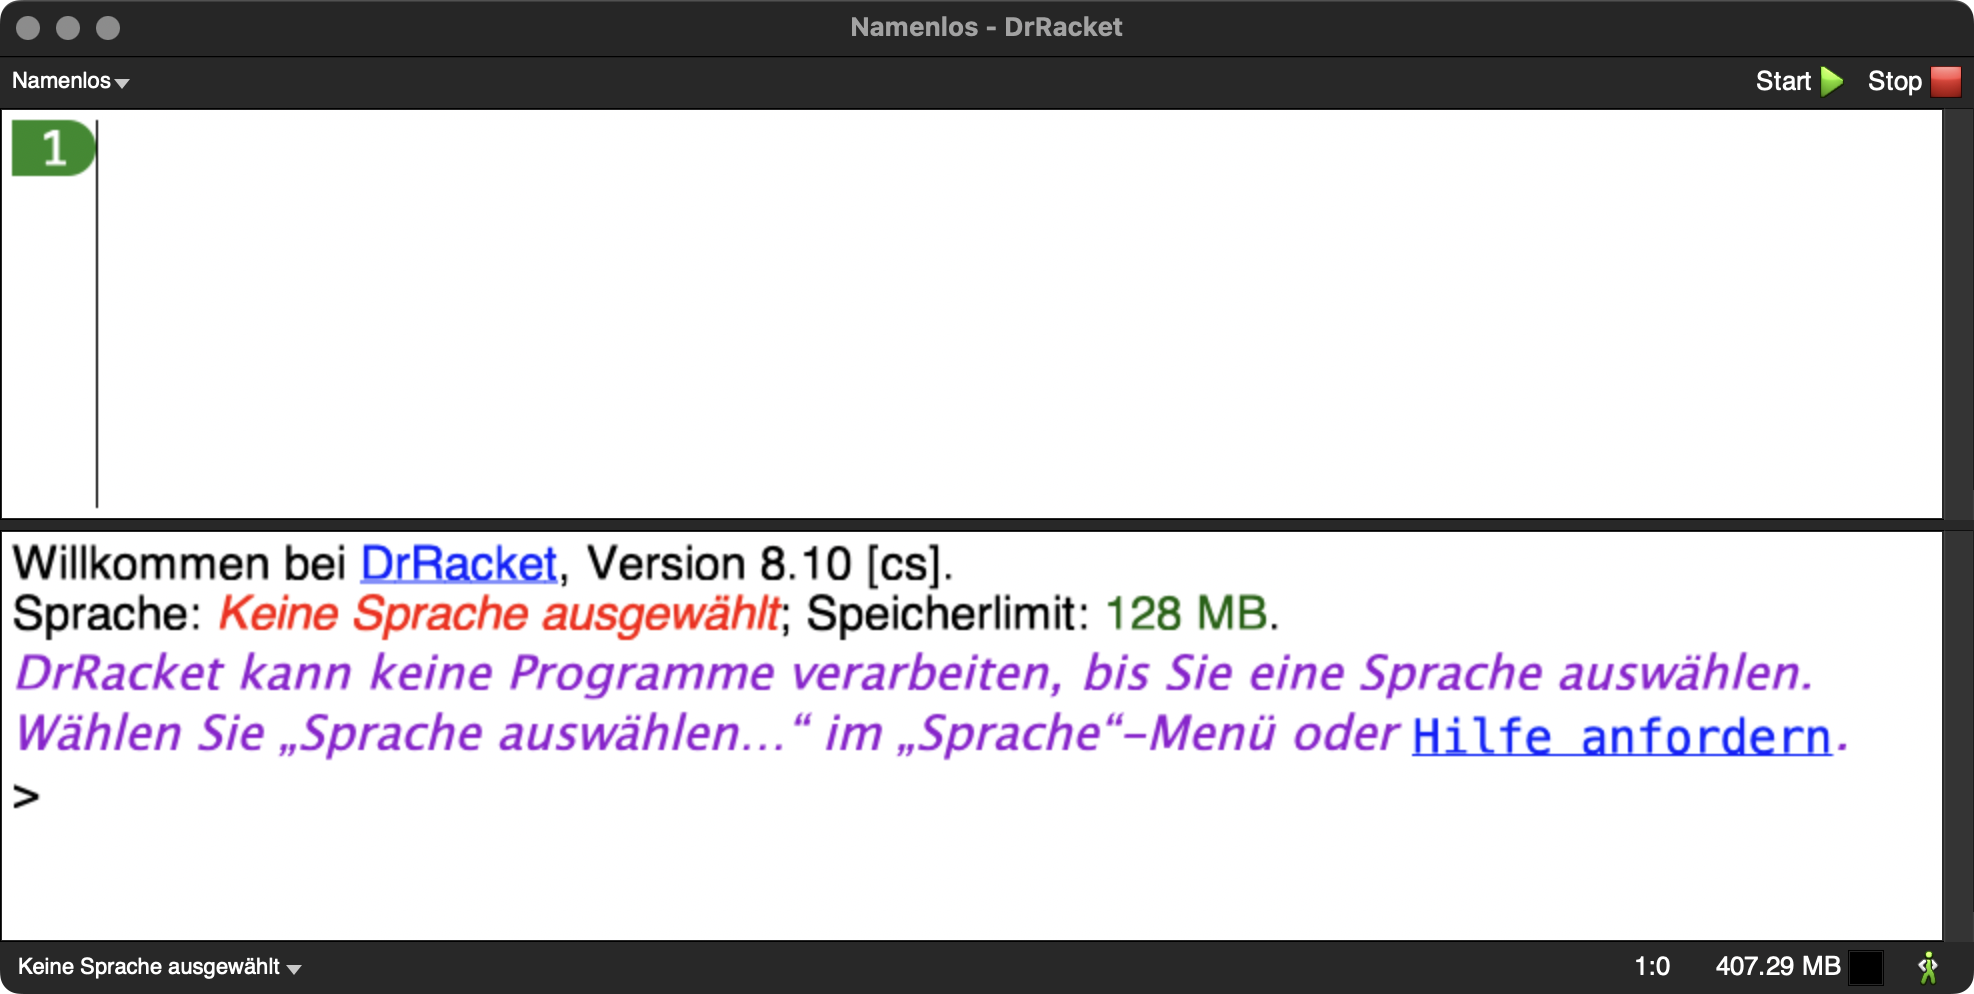
\includegraphics[width=\textwidth]{elemente/drracket-start}
  \caption{DrRacket nach dem ersten Start}
  \label{fig:drracket-start}
\end{figure}

Zu Racket gehört ein Programm namens
\textit{DrRacket}\index{DrRacket}: starte es.  Es erscheint ein
Fenster, das ungefähr so aussehen sollte wie in
Abbildung~\ref{fig:drracket-start}.  Die Benutzeroberfläche kannst
Du auf Deutsch umstellen, indem Du im \texttt{Help}-Menü auf \texttt{Deutsche
  Benutzeroberfläche für DrRacket} drückst.  Wenn Du die Auswahl
bestätigst, wird DrRacket danach beendet und Du musst es noch einmal
starten; dann sollten die Menüs auf Deutsch sein.

DrRacket ist eine \textit{Entwicklungsumgebung}, mit der Du Programme
schreiben und ausführen kannst.  DrRacket unterstützt nicht nur eine
einzige Programmiersprache, sondern viele.
Darum musst Du die richtige Programmiersprache für
dieses Buch noch auswählen.  Wähle dazu den Menüpunkt
\texttt{Sprache $\rightarrow$ Sprache auswählen} (\texttt{Language $\rightarrow$ Choose language} in der englischen
Fassung), worauf ein neues Fenster mit einem Dialog erscheint.
In dem Dialog gibt es eine
Abteilung \texttt{Lehrsprachen\index{Lehrsprachen}}, und darunter eine
Überschrift namens \texttt{DeinProgramm}, unterhalb dessen mehrere
Einträge erscheinen, die speziell auf die Kapitel dieses Buchs
zugeschnitten sind.

\begin{figure}[tb]
  \centering
  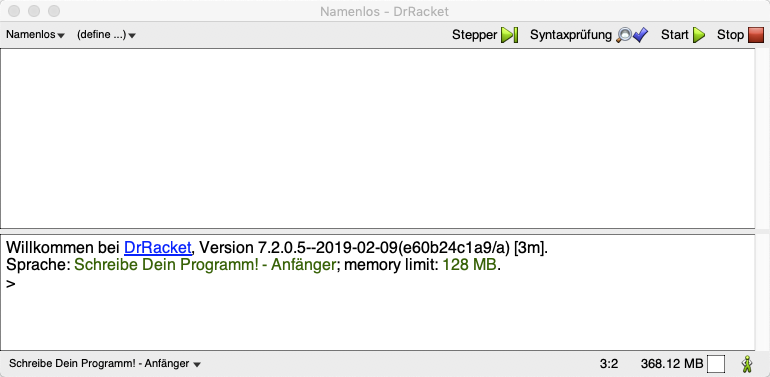
\includegraphics[width=\textwidth]{elemente/drracket-deinprogramm}
  \caption{DrRacket mit ausgewählter Lehrsprache}
  \label{fig:drracket-deinprogramm}
\end{figure}

Für den ersten Teil des Buchs ist die Ebene \texttt{Schreibe Dein
  Programm! - Anfänger} zuständig:\index{Sprachebene!Anfänger} Wähle
diese aus und drücke dann einmal oben rechts auf den Knopf
\texttt{Start} (beziehungsweise \texttt{Run}), damit die Auswahl aktiv wird.
Das Ergebnis sollte dann so aussehen wie in
Abbildung~\ref{fig:drracket-deinprogramm}.

Das DrRacket-Fenster besteht aus zwei Teilen:
%
\begin{enumerate}
\item In der oberen Hälfte des Fensters (dem
  \textit{Editor-\index{Editor}} oder
  \textit{Definitionsfenster\index{Definitionsfenster}}) steht der
  Programmtext.  Der Editor funktioniert ähnlich wie ein reguläres
  Textverarbeitungsprogramm.  Was dort steht, kannst Du abspeichern.
  Wenn Du ein Programm abspeicherst, benutze die Endung \texttt{.rkt}
  für "<\textbf{R}ac\textbf{k}e\textbf{t}">.
\item In der unteren Hälfte des Fensters~-- dem
  \textit{Interaktionsfenster\index{Interaktionsfenster}} oder der
  sogenannten \textit{REPL\index{REPL}}\footnote{"<REPL"> steht für
    "<Read-Eval-Print-Loop">~-- wir werden später zeigen, warum.}
  werden die Ausgaben des Programms angezeigt.  Außerdem kannst Du
  einzelne Programmteile gezielt testen.
\end{enumerate}
%

\section{Ausdrücke und die REPL}

Fangen wir mit der REPL an: Wenn Du gerade \texttt{Start} gedrückt
hast, dann erscheint der Cursor rechts von dem \lstinline{>}-Zeichen:
Hier kannst Du etwas eingeben und Return drücken.  DrRacket zeigt dann
das Ergebnis darunter an.

Wenn Du zum Beispiel \lstinline{123} eintippst, zeigt DrRacket gleich
darunter 123 an.  DrRacket kann auch rechnen.  Dafür musst Du
allerdings die Rechenaufgaben etwas anders aufschreiben als sonst.
Zum Beispiel so:
%
\begin{lstlisting}
(+ 123 42)
\end{lstlisting}
%
Wenn Du das in die REPL eingibst, zeigt DrRacket \lstinline{165} an, die
\textit{Summe}\index{Summe} von 123 und 42.  Diese "<Rechenaufgabe">
ist ein sogenannter \textit{Ausdruck\index{Ausdruck}}.  Ausdrücke, die
etwas ausrechnen sollten, haben in den Lehrsprachen immer die gleiche
Form:
%
\begin{lstlisting}
(|\textnormal{\textit{Operator}}| |\textnormal{\textit{Operand}}| |\ldots|)
\end{lstlisting}
%
Es stehen \emph{immer} Klammern\index{Klammer} drumherum
(und die können auch nirgendwo sonst stehen).  Dann folgt der
\textit{Operator\index{Operator}}, der bestimmt, \emph{was} gemacht
wird (die \textit{Operation}).  Danach kommen die
\textit{Operanden\index{Operand}}, welche die Eingaben\index{Eingabe}
für die Operation bestimmen.

Zum Merken ist es hilfreich, Ausdrücke entsprechend vorzulesen: Also
nicht mehr "<hundertdreiundzwanzig plus zweiundvierzig">, sondern
"<die \emph{Summe} von hundertdreiundzwanzig und zweiundvierzig">.

Wenn Du Klammern vergisst,
können verwirrende Ergebnisse herauskommen.  Wenn Du zum Beispiel
\lstinline{+ 123 42} in der REPL eintippst, sieht das so aus:
%
\begin{alltt}
> + {\color{DarkGreen}123 42}
{\color{blue}#<function:+>
123
42}
\end{alltt}
%
Das liegt daran, dass ohne Klammern \lstinline{+ 123 32} aus \emph{drei}
Ausdrücken besteht und die REPL deshalb auch drei Ergebnisse ausdruckt:
Die Funktion \lstinline{+}, dann die \lstinline{123}, dann \lstinline{42}.
(Die Operation \lstinline{+} ist eine sogenannte Funktion~-- das
erläutern wir später noch genauer.)  Ähnlich verhält es sich mit
\lstinline{123 + 42}~-- probiere es aus!

Wenn Du versehentlich die Klammern setzt, aber den Operator dazwischen
schreibst, erscheint in der REPL eine Fehlermeldung:
%
\begin{alltt}
> ({\color{DarkGreen}123} + {\color{DarkGreen}42})
{\color{red}Operator darf keine Zahl sein, ist aber 123}
\end{alltt}
%
Etwas ähnliches passiert, wenn das Leerzeichen zwischen dem
Operator und den Operanden fehlt~-- oder zwischen den Operanden.  Das
sieht zum Beispiel so aus:
%
\begin{alltt}
> ({\color{DarkGreen}+123} {\color{DarkGreen}42})
{\color{red}Operator darf keine Zahl sein, ist aber 123}
\end{alltt}
%
Das liegt daran, dass \lstinline{+123} zusammen die Zahl "<plus
hundertdreiundzwanzig"> bildet und nicht etwa in das \lstinline{+}-Zeichen und
\lstinline{123} aufgeteilt wird.

Wenn ein Ausdruck wie \lstinline{(+ 123 42)} ein Ergebnis wie 165 hat,
schreiben wir das im Buch zukünftig so, etwas anders als die
DrRacket-REPL:
%
\begin{lstlisting}
(+ 123 42)
|\evalsto| 165
\end{lstlisting}
%
So lassen sich natürlich nicht nur Summen, sonderen auch Differenzen,
Produkte (mit dem Operator \lstinline{*}) und Quotienten (mit dem
Operator \lstinline{/}) ausrechnen:
%
\begin{lstlisting}
(- 123 42)
|\evalsto| 81
(* 123 42)
|\evalsto| 5166
(/ 123 42)
|\evalsto| 2.9$\overline{\mathtt{285714}}$
\end{lstlisting}
%
Beim letzen Ausdruck ist zu sehen, dass Dezimalzahlen mit Punkt und
nicht mit Komma geschrieben werden.  Der Überstrich bei
\lstinline{2.9$\overline{\mathtt{285714}}$} ist eine
\textit{Periode\index{Periode}}. Die Zahl ist also eigentlich
%
\begin{lstlisting}
2.9285714285714285714285714285714|\ldots|
\end{lstlisting}
%
Die REPL funktioniert also folgendermaßen: Sie \emph{liest} einen
Ausdruck ein (auf Englisch "<read">), berechnet dessen Wert oder \emph{wertet}
diesen \emph{aus} ("<eval">, kurz für "<evaluate">) und zeigt das Ergebnis an
oder \emph{druckt} dieses \emph{aus} ("<print">)~-- und dann geht es
von vorn los, wie in einer Schleife ("<loop">).  Die Abfolge
\emph{Read-Eval-Print-Loop} gibt der REPL ihren Namen.

Ausdrücke können auch kombiniert werden, zum Beispiel so:
%
\begin{lstlisting}
(* 123 (+ 20 22))
|\evalsto| 5166
(* 123 (+ (* 2 10) 22))
|\evalsto| 5166
\end{lstlisting}
%
Bei der Kombination verschiedener Ausdrücke ist es wichtig,
dass um jeden Teilausdruck wieder ein
Klammernpaar kommt.  Ist das nicht der Fall, erscheinen gelegentlich
auch mal Fehlermeldungen wie diese hier:
%
\begin{lstlisting}
(* 123 (+ * 2 10 22))
|\color{red}\texttt{+: Zahl als erstes Argument erwartet, \#<function:*> bekommen}|
\end{lstlisting}
%
Das liegt daran, dass das \lstinline{*} hier an der Stelle eines
Operanden steht.  Das Wort \textit{Argument} steht für
den Wert des Operanden einer Funktion, darum steht da sinngemäß, dass
\lstinline{+} eine Zahl als erstes Argument etwartet, aber
stattdessen die Funktion \lstinline{*} bekommen hat.  (Das Wort
"<Argument"> definieren wir genauer in Abschnitt~\ref{sec:argument} auf
Seite~\pageref{sec:argument}.)

Abspeichern geht mit der REPL nicht, und der REPL-Inhalt verschwindet
auch jedesmal, wenn Du \texttt{Start} beziehungsweise \texttt{Run} drückst.  Du
kannst aber frühere Eingaben zurückholen, indem Du
\texttt{Strg-$\uparrow$} beziehungsweise \texttt{Control-$\uparrow$}
(je nach Computertyp) drückst.  (Das geht natürlich auch nach unten
mit \texttt{Strg-$\downarrow$} beziehungsweise
\texttt{Control-$\downarrow$}.)
Das kannst Du auch benutzen, um einen
fehlerhaften Ausdruck zu korrigieren, bei dem Du schon Return gedrückt hast.

\begin{aufgabeinline}
  Schreibe folgende "<mathematischen"> Ausdrücke in der Notation der
  Lehrsprache in die REPL und lasse die REPL sie auswerten:
  %
  \begin{displaymath}
    \begin{array}{c}
      55 * 27\\
      23 * (44 + 27)\\
      \frac{23}{44} + \frac{44}{23}\\
      (23 + 42) * (12 + (14 * 2))
    \end{array}
  \end{displaymath}
\end{aufgabeinline}
%
\section{Das Definitionsfenster}

Kommen wir zum Definitionsfenster oben.  Dort schreibst Du Dein
Programm, die REPL kannst Du dann benutzen, um es auszuprobieren.
Schreib in das Definitionsfenster folgende
\textit{Definition\index{Definition}}:
%
\begin{lstlisting}
(define alles (+ 20 22))
\end{lstlisting}
%
Diese Definition besagt, dass der Name \lstinline{alles} für das Ergebnis
von \lstinline{(+ 20 22)} steht.  Um das auszuprobieren, drück auf den
Knopf \texttt{Start} beziehungsweise \texttt{Run} rechts oben.  Der Cursor
landet dann wieder in der REPL, wo Du das Programm ausprobieren
kannst:
%
\begin{lstlisting}
alles
|\evalsto| 42
\end{lstlisting}
%
Ein solcher Name in einem Programm heißt
\textit{Variable\index{Variable}}.\footnote{Obwohl der Begriff
  "<Variable"> suggeriert, dass etwas daran verändert werden
  kann, bleibt der Wert einer Variable immer gleich.}

Hier sind ein paar weitere Beispiele für Definitionen von Variablen:
%
\begin{lstlisting}
(define one 1)
(define temperature 23)
(define birgit-prinz 9)
\end{lstlisting}
%
Du kannst auch diese Namen in die REPL eingeben und bekommst
jeweils den dazugehörigen Wert, wenn Du Return drückst:
%
\begin{lstlisting}
one
|\evalsto| 1
temperature
|\evalsto| 23
birgit-prinz
|\evalsto| 9
\end{lstlisting}
%
Bei der Gestaltung eines Namens gibt es weitgehende Freiheiten. Anders
als in anderen Programmiersprachen sind auch Bindestriche in Namen
möglich.  Nur Leerzeichen sind nicht erlaubt.

Groß- und Kleinschreibung ist bei Namen egal.  Es funktioniert also
auch:
%
\begin{lstlisting}
Alles
|\evalsto| 42
ONE
|\evalsto| 1
tEmPeRaTuRe
|\evalsto| 23
\end{lstlisting}
%
In einem Programm kannst Du Zeilenumbrüche und Einrückung benutzen, um
Dein Programm übersichtlicher zu gestalten.  Zum Beispiel kannst Du
nach \lstinline{alles} die Return-Taste drücken, das Ergebnis sieht so
aus:
%
\begin{lstlisting}
(define alles
  (+ 20 22))
\end{lstlisting}
%
DrRacket rückt die zweite Zeile ein bisschen ein, um auszudrücken,
dass sie noch in die Klammern vom \lstinline{define} gehört.  Bei
komplizierteren Ausdrücken ist das hilfreich:
%
\indexvariable{alles}
\begin{lstlisting}
(define alles
  (+ 20
     (* 11 2)))
\end{lstlisting}
%
Hier stellt DrRacket die Operanden der Summe genau untereinander.
DrRacket zwingt Dich nicht, die Einrückung genau so zu machen, und
durch Änderungen im Programm gerät sie auch manchmal aus dem Lot.  In
dem Fall kannst Du die Tab-Taste drücken (auf den meisten Tastaturen
steht $\longrightarrow\mid$ auf der Tab-Taste) und in der Zeile, in
welcher der Cursor steht, wird die Einrückung korrigiert.
Wenn Du einen Abschnitt im Programm markierst und dann Tab drückst,
wird der ganze Abschnitt neu eingerückt.  
Es gibt
außerdem einen Menüpunkt \texttt{Racket $\rightarrow$ Alles einrücken} (beziehungsweise
\texttt{Racket $\rightarrow$ Reindent All}), der das für das gesamte
Programm macht.

Ein weiterer praktischer Trick ist, dass Du einen geklammerten
Ausdruck markieren (und dann ausschneiden) kannst, indem Du auf die
öffnende oder schließende Klammer doppelt klickst.  Insbesondere
kannst Du den markierten Ausdruck dann mit einem Druck auf die
Tab-Taste korrekt einrücken.

\begin{aufgabeinline}
  Bring bei einem mehrzeiligen Programm die Einrückung richtig
  durcheinander, zum Beispiel so:
\begin{lstlisting}
(define nr
  (+ 12
 (- (* 42
  13)
    500)))
\end{lstlisting}
  %
  Benutze dann die Tab-Taste, um die Einrückung wieder zu korrigieren.
\end{aufgabeinline}
%
Den Inhalt des Definitionsfensters kannst Du abspeichern, indem Du auf
den Knopf mit dem Diskettensymbol
\raisebox{-1ex}{
\includegraphics[height=12pt]{elemente/save}}\footnote{Disketten
wurden im 20.~Jahrhundert verwendet, um Daten zu speichern.  Es gab
damals noch keine Speicherkarten oder USB-Sticks.}
drückst.  Du bekommst dann ein Dialogfenster, in dem Du einen
Dateinamen vergeben kannst.

\section{Rechnen ohne Zahlen}

Computerprogramme können nicht nur mit Zahlen rechnen.  In diesem
Abschnitt geht es um das Rechnen mit Text und das Rechnen mit Bildern.

\subsection{Rechnen mit Text}

Aus Text\index{Text} kann durch doppelte Anführungszeichen ein Wert werden:
%
\begin{lstlisting}
"Mike Sperber"
"Herbert Klaeren"
"Schreibe Dein Programm!"
\end{lstlisting}
%
Solche Text-Werte heißen \textit{Zeichenketten\index{Zeichenkette}}.

Die einfachste Art, eine Zeichenkette herzustellen, ist, die
Buchstaben hinzuschreiben, aus denen sie besteht.  Die
Anführungszeichen müssen drumherum, damit die Zeichenketten von anderen
Ausdrücken unterschieden werden können.  Die Anführungszeichen gehören aber nicht
zu den Buchstaben dazu, aus denen die Zeichenkette besteht~--
\lstinline{"abc"} besteht aus den drei Buchstaben \texttt{abc}.

\begin{feature}{Zeichenketten}{scheme:strings}
\textit{Zeichenketten\index{Zeichenkette}} (auf Englisch
\textit{Strings}\index{String}) repräsentieren Text.
Literale für Zeichenketten haben folgende Form:
%
\begin{lstlisting}
"$z\sb{1}$$z\sb{2}$ $\ldots$ $z\sb{n}$"
\end{lstlisting}
%
Dabei sind die \(z\sb{i}\) beliebige einzelne Zeichen, außer \lstinline{"} selbst.
Beispiel:
%
\begin{lstlisting}
"Herbert was here!"
\end{lstlisting}
%
Das Anführungszeichen (\lstinline{"}) kann nicht "<ungeschützt"> vorkommen, da es das Ende der
Zeichenkette markiert. Es wird als "<echtes"> Anführungszeichen innerhalb einer Zeichenkette
durch \lstinline{\"} dargestellt:
%
\begin{lstlisting}
"Herbert sagt |\backwhack|"Hallo Mike|\backwhack|"!"
\end{lstlisting}
\end{feature}

Abbildung~\ref{scheme:strings} beschreibt die genaue Schreibweise für
solche "<festen"> Zeichenketten.  Feste Schreibweisen für Werte heißen
allgemein \textit{Literale\index{Literal}}.  Das kennen wir schon von
den Zahlen: Die Zeichenfolge \lstinline{123} steht für die Zahl
"<hundertdreiundzwanzig">.  Kästen wie Abbildung~\ref{scheme:strings}
werden in diesem Buch noch oft dazu dienen, neue Sprachelemente
einzuführen.

Mit Text kann ein Programm auch rechnen, und zwar mit der eingebauten
Funktion
\texttt{string"=append}\indexvariable{string-append},
die zwei Zeichenketten aneinanderhängt:
%
\begin{lstlisting}
(string-append "Herbert" "Mike")
|\evalsto| "HerbertMike"
(string-append "Mike" " " "ist doof")
|\evalsto| "Mike ist doof"
\end{lstlisting}
%
Die eingebaute Funktion
\lstinline{string-length}\indexvariable{string-length}
liefert die Anzahl der Zeichen in einer Zeichenkette:
%
\begin{lstlisting}
(string-length "Herbert")
|\evalsto| 7
(string-length "Mike")
|\evalsto| 4
\end{lstlisting}
%
Die Namen \lstinline{string-append} und \lstinline{string-length} sehen auf
den ersten Blick "<anders"> aus als \lstinline{+} und \lstinline{*} zum
Beispiel, dieser Eindruck täuscht jedoch: Sie sind allesamt Namen von
vordefinierten Operationen, die Programme benutzen können, ohne sie
selbst definieren zu müssen.

Die vordefinierten Funktionen
\lstinline{string->number}\indexvariable{string->number}
und \lstinline{number->string} konvertieren zwischen Zahlen und den
Zeichenketten, die diese darstellen:
%
\begin{lstlisting}
(string->number "23")
|\evalsto| 23
(number->string 23)
|\evalsto| "23"
\end{lstlisting}
%
\begin{aufgabeinline}
  Mache Dir den Unterschied zwischen der Zahl \lstinline{23} und der
  Zeichenkette \lstinline{"23"} klar.  Probiere zum Beispiel aus:
\begin{lstlisting}
(+ "23" 42)
(string-append 23 "42")
(number->string "23")
\end{lstlisting}
\end{aufgabeinline}

\subsection{Rechnen mit Bildern}
\label{sec:rechnen-mit-bildern}

Programme können auch mit Bildern rechnen.  Dazu wird eine Erweiterung
zu DrRacket benötigt, ein sogenanntes
\textit{Teachpack}\index{Teachpack}.  Um es zu aktivieren, wähle den Menüpunkt
\texttt{Sprache $\rightarrow$ Teachpack hinzufügen}
(\texttt{Language $\rightarrow$ Add Teachpack}).  In dem folgenden Dialog
wähle \texttt{image.rkt} aus und drücke 
\texttt{OK}.  Dann musst Du noch einmal auf \texttt{Start} drücken.
Wenn alles geklappt hat, steht unten in der REPL
\texttt{Teachpack: image.rkt}.

Das Teachpack \texttt{image.rkt} enthält zusätzliche vordefinierte
Funktionen, mit denen wir Bilder herstellen können.  Zum Beispiel
\lstinline{square}, \lstinline{circle} und \lstinline{star-polygon}:
%
\begin{lstlisting}
(square 40 "solid" "red")
|\evalsto| |
\includegraphics[height=24pt]{elemente/square}|
(circle 20 "solid" "green")
|\evalsto| |
\includegraphics[height=24pt]{elemente/circle}|
(star-polygon 20 10 3 "solid" "blue")
|\evalsto| |
\includegraphics[height=24pt]{elemente/starpolygon}|
\end{lstlisting}
%
Schauen wir uns das eingebaute \lstinline{star-polygon} etwas näher an:
Es akzeptiert fünf Eingaben, die ersten drei davon sind Zahlen~-- die
Seitenlänge, die Seitenanzahl und die Anzahl der Ecken, die für jede
Seite übersprungen wird.  Danach kommen zwei Zeichenketten~--
\lstinline{"solid"} heißt, dass das Innere des Sterns ausgefüllt ist und
\lstinline{"blue"} ist die Farbe.  Statt \lstinline{"solid"} kannst Du auch
\lstinline{"outline"} schreiben, dann wird auch etwas klarer, was
"<überspringen"> heißt:
%
% filename can't contain hyphen because of alltt
\begin{lstlisting}
(star-polygon 20 10 3 "outline" "blue")
|\evalsto| |
\includegraphics[height=24pt]{elemente/starpolygon_outline}|
\end{lstlisting}
%
\begin{aufgabeinline}
  Wofür stehen die Zahleneingaben bei \lstinline{square} und
  \lstinline{circle}?  Probiere unterschiedliche Zahlen aus!  Es gibt
  auch eine eingebaute Funktion \lstinline{rectangle}.  Kannst Du ein
  funktionierendes Beispiel für den Einsatz von \lstinline{rectangle}
  konstruieren?  Außerdem gibt es eine eingebaute Funktion
  \lstinline{ellipse}, die genauso benutzt wird wie \lstinline{rectangle}~--
  probiere sie aus!
\end{aufgabeinline}
%
Bilder sind Werte wie Zahlen und Zeichenketten auch.  Du kannst
mit Definitionen auch Namen dafür vergeben:
%
\begin{lstlisting}
(define s1 (square 40 "solid" "red"))
(define c1 (circle 40 "solid" "green"))
(define p1 (star-polygon 20 10 3 "solid" "blue"))
\end{lstlisting}
%
\begin{aufgabeinline}
  Probiere diese Definitionen in der REPL aus, indem Du dort
  \lstinline{s1}, \lstinline{c1} und \lstinline{p1} eingibst.  Was
  passiert, wenn Du \lstinline{(s1)} eingibst?  Warum?
\end{aufgabeinline}

\begin{aufgabeinline}
  Du kannst auch Bilddateien oder Bilder von Webseiten in Dein Programm
  einfügen, wie in einem Textverarbeitungsprogramm. Das geht so:
  %
  \begin{itemize}
    \item Um eine Bilddatei einzufügen, wähle den Menüpunkt
      \texttt{Einfügen $\rightarrow$ Bild einfügen} beziehungsweise
      \texttt{Insert $\rightarrow$ Insert Image}.
    \item Um ein Bild aus einer Webseite einzufügen, wähle aus dem
      Kontextmenü im Browser \texttt{Bild kopieren} (oder \texttt{Copy
      Image} oder so ähnlich) aus.  Du kannst das Bild dann in
    DrRacket über den Menüpunkt \texttt{Bearbeiten $\rightarrow$ Einfügen}
    beziehungsweise \texttt{Edit $\rightarrow$ Paste} einfügen.
  \end{itemize}
  %
  Probier es aus und
  gib dem Bild einen Namen!
\end{aufgabeinline}
%
Mit Bildern kann DrRacket auch rechnen:\label{function:beside-above}
%
\begin{lstlisting}
(beside s1 p1)
|\evalsto| |
\includegraphics[height=24pt]{elemente/beside.png}|
(above s1 c1)
|\evalsto| |
\includegraphics[width=24pt]{elemente/above.png}|
(above (beside s1 p1) (beside p1 c1))
|\evalsto| |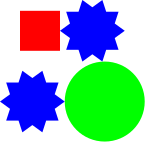
\includegraphics[width=48pt]{elemente/abovebeside.png}|
\end{lstlisting}
%
\begin{aufgabeinline}
  Probiere in der REPL folgende Ausdrücke aus:
\begin{lstlisting}
(triangle 50 "outline" "red")
(square 100 "solid" "blue")
\end{lstlisting}
  %
  Schreibe mit Hilfe der Funktionen \lstinline{triangle} und
  \lstinline{square} einen Ausdruck, der ein ganz einfaches Haus
  berechnet.
\end{aufgabeinline}
%
Das heißt, \lstinline{above} akzeptiert als Eingabe zwei (oder mehr)
Bilder und macht daraus wieder ein Bild, in dem die Teilbilder
übereinander stehen.  Das gleiche gilt für \lstinline{beside}, nur dass
die Bilder nebeneinander angeordnet werden.  Selbstverständlich können
\lstinline{above} und \lstinline{beside} auch kombiniert werden.

\section{Abstraktion und Applikation}
\label{sec:abstraktion-und-applikation}

\mentioncode{elemente/tile.rkt}
%
Hier sind zwei Ausdrücke, welche die Bilder aus dem vorigen Abschnitt
zu einem Muster kombinieren:
%
\begin{lstlisting}
(above
 (beside s1 p1)
 (beside p1 s1))
|\evalsto| |
\includegraphics[width=48pt]{elemente/tile1}|

(above
 (beside p1 c1)
 (beside c1 p1))
|\evalsto| |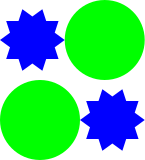
\includegraphics[width=48pt]{elemente/tile2}|
\end{lstlisting}
%
Beide Ausdrücke folgen dem gleichen Muster, sie "<kacheln"> jeweils zwei
Bilder in einer quadratischen Anordnung.  Das Muster könnte man so
hinschreiben:
%
\begin{lstlisting}
(above
 (beside a b)
 (beside b a))
\end{lstlisting}
%
Das erste Beispiel entsteht, indem für \lstinline{a} \lstinline{s1}
eingesetzt wird und für \lstinline{b} \lstinline{p1}, im zweiten für \lstinline{a}
\lstinline{p1} und für \lstinline{b} dann \lstinline{c1}.

Dieses Muster kannst Du in ein Programm gießen.  Dann müssen wir nicht
jedesmal \lstinline{above} ~\ldots~ \lstinline{beside} ~\ldots~ \lstinline{beside} eintippen.
Dazu schreibst Du es erst einmal genauso hin, also mit \lstinline{a} und
\lstinline{b}.  Wenn es startet, erscheint folgende Meldung:
%
\begin{alltt}
\color{red}a: Variable ist nicht definiert
\end{alltt}
%
Das bedeutet, dass es keine Definition für \lstinline{a} gibt.
Du könntest eine hinschreiben, zum Beispiel:
%
\begin{lstlisting}
(define a s1)
\end{lstlisting}
%
Aber dann wäre \lstinline{a} auf \lstinline{s1} festgelegt.  Wir wollen
stattdessen das Muster verallgemeinern, so dass Du es mehrmals mit
unterschiedlichen Werten für \lstinline{a} und \lstinline{b} verwenden
kannst.  Dieser Verallgemeinerungsprozess heißt beim Programmieren
\textit{Abstraktion\index{Abstraktion}}.  Dafür müssen wir dem Muster
noch etwas hinzufügen, um zu sagen, dass wir unterschiedliche Werte
für \lstinline{a} und \lstinline{b} einsetzen wollen:
%
\begin{lstlisting}
(lambda (a b)
  (above
   (beside a b)
   (beside b a)))
\end{lstlisting}
%
Das \lstinline{lambda}\indexvariable{lambda} ist eine Art Zauberwort, es sagt soviel wie: "<Für
die Variablen \lstinline{a} und \lstinline{b} möchte ich später (und
vielleicht mehrmals) Werte einsetzen.">  Wenn Du das Programm jetzt
startest, geht die Fehlermeldung weg und in der REPL erscheint:
%
\begin{lstlisting}
#<function>
\end{lstlisting}
%
Das deutet darauf hin, dass bei dem \lstinline{lambda} eine Funktion
herauskommt.  Um etwas damit anzufangen, gib ihr einen Namen mit
\lstinline{define}:
%
\indexvariable{tile}
\begin{lstlisting}
(define tile
  (lambda (a b)
    (above
     (beside a b)
     (beside b a))))
\end{lstlisting}
%
(Alles schön richtig einrücken! "<To tile"> heißt auf Deutsch
"<kacheln">.\footnote{Wir mögen gern englischsprachige Namen für
  Variablen.  Das ist aber eine rein persönliche Präferenz~-- gern
  kannst Du deutschsprachige Variablen für Deine eigenen Programme
  verwenden.})

Dadurch ist eine neue Operation entstanden.  Die kannst Du direkt
verwenden:
%
\begin{lstlisting}
(tile s1 p1)
|\evalsto| |
\includegraphics[width=48pt]{elemente/tile1}|

(tile p1 c1)
|\evalsto| |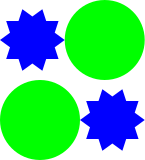
\includegraphics[width=48pt]{elemente/tile2}|
\end{lstlisting}
%
Was ist da passiert?  Am einfachsten kann man das in einem speziellen
Werkzeug sehen, dem \textit{Stepper\index{Stepper}}.  Um ihn zum
Einsatz zu bringen, stelle sicher, dass im Definitionsfenster folgendes
Programm steht:
%
\begin{lstlisting}
(define s1 (square 40 "solid" "red"))
(define c1 (circle 40 "solid" "green"))
(define p1 (star-polygon 20 10 3 "solid" "blue"))

(define tile
  (lambda (a b)
    (above
     (beside a b)
     (beside b a))))

(tile s1 p1)
(tile p1 c1)
\end{lstlisting}
%
Dann drück auf den \texttt{Stepper}-Knopf (beziehungsweise
\texttt{Step} in der englischen Fassung) oben rechts im
DrRacket-Fenster.  Es erscheint ein neues Fenster, das so aussieht:

\begin{figure}[H]
  \centering
  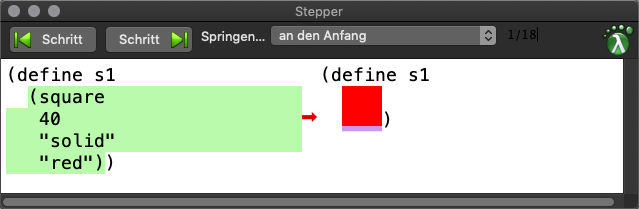
\includegraphics[width=0.6\textwidth]{elemente/stepper-0}
  \caption{Der Stepper in Aktion}
  \label{fig:stepper-0}
\end{figure}
%
\noindent Wenn Du jetzt den Knopf mit dem Vorwärts- beziehungsweise
dem Rückwärts-Pfeil drückst, kannst Du zusehen, wie DrRacket Dein
Programm ausführt.  Wenn Du ein paar Schritte vorwärts gehst, sieht
das so aus:
%
\begin{figure}[H]
  \centering
  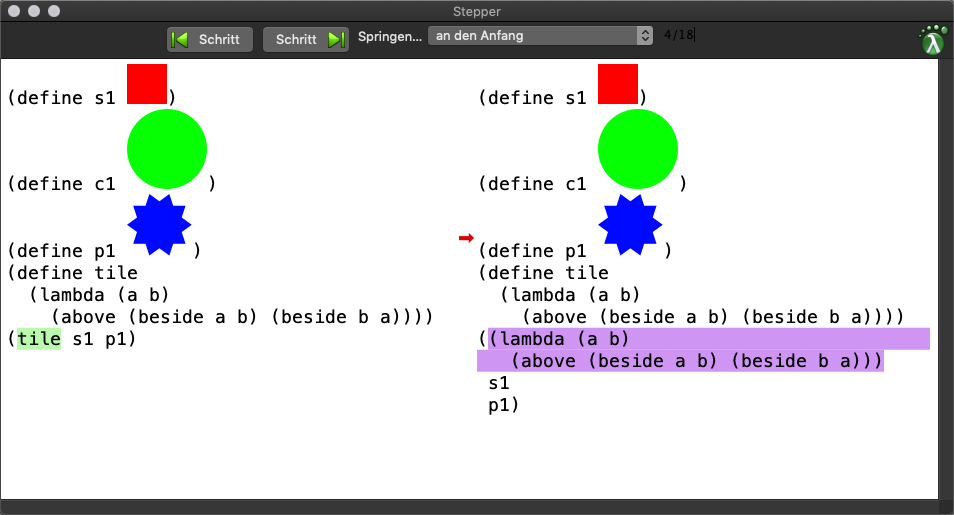
\includegraphics[width=0.8\textwidth]{elemente/stepper-1}
  \caption{Stepper: Variable ersetzen}
  \label{fig:stepper-1}
\end{figure}
%
\noindent Du kannst sehen, wie DrRacket jeweils einen Schritt auf
einmal auswertet~-- der ist auf der linken Seite grün~-- und dann
rechts durch das Resultat ersetzt.  Oben kannst Du sehen, wie der
Stepper die Variable \lstinline{tile} durch den \lstinline{lambda}-Ausdruck
aus der Definition von \lstinline{tile} ersetzt. Das macht der Stepper
auch mit den Definitionen von \lstinline{s1} und \lstinline{p1}:
%
\begin{figure}[H]
  \centering
  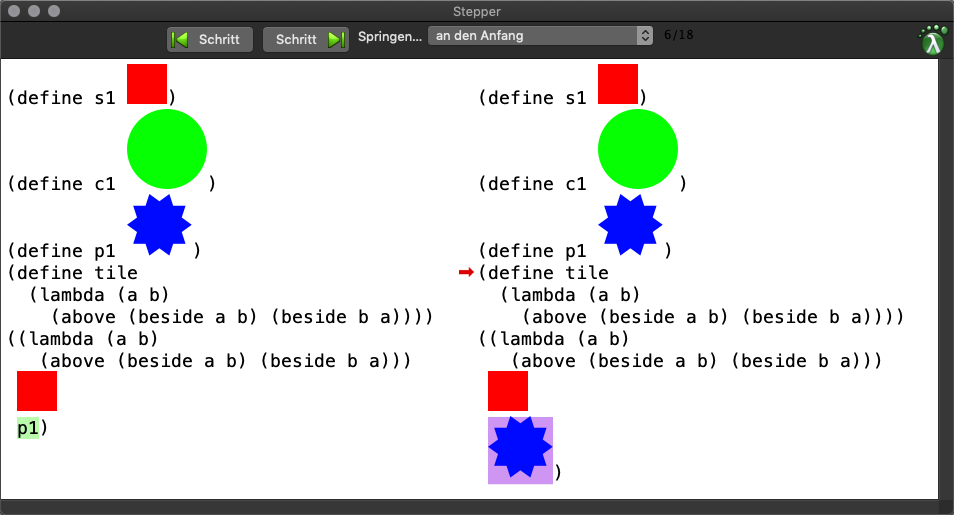
\includegraphics[width=0.8\textwidth]{elemente/stepper-2}
  \caption{Stepper: Variable}
  \label{fig:stepper-2}
\end{figure}
%
\noindent Interessant wird es danach. Die Variablen aus den Definitionen sind
alle ersetzt.  Hinter dem \lstinline{lambda}-Ausdruck stehen jetzt das
Quadrat und der Stern, und die werden jetzt für die Variablen aus dem
\lstinline{lambda}-Ausdruck eingesetzt, also das Quadrat für \lstinline{a}
und der Stern für \lstinline{b}:
%
\begin{figure}[H]
  \centering
  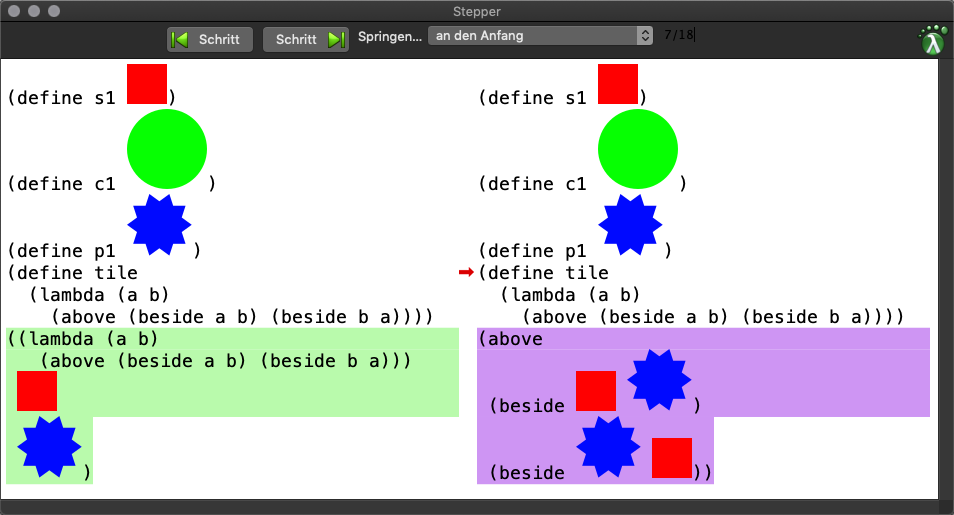
\includegraphics[width=0.8\textwidth]{elemente/stepper-3}
  \caption{Stepper: Applikation}
  \label{fig:stepper-3}
\end{figure}
%
\noindent Dabei verschwindet auch das \lstinline{lambda}.
%
\begin{aufgabeinline}
  Probiere das Beispiel im Stepper aus und klicke Dich bis zum Ende
  durch. Mache Dir dabei klar, wie jeweils die linke mit der rechten
  Seite zusammenhängt.
\end{aufgabeinline}
%
\lstinline{(tile s1 p1)} ist eine sogenannte
\textit{Applikation\index{Applikation}}: ein Ausdruck mit
Klammern drum.  Der Operator und die Operanden der
Applikation sind ebenfalls Ausdrücke.  Der Operator ergibt eine
Funktion~-- entweder eingebaut oder aus einem
\lstinline{lambda}-Ausdruck.  Eine Applikation wird auch oft
\textit{Funktionsaufruf\index{Funktionsaufruf}} oder
\textit{Funktionsanwendung\index{Funktionsanwendung}} genannt.

Wenn die Funktion ein \lstinline{lambda}-Ausdruck ist wie in
Abbildung~\ref{fig:stepper-3}, dann muss es genauso viele Operanden
geben wie der \lstinline{lambda}-Ausdruck Variablen hat.
Dann wertet DrRacket den Ausdruck wie folgt aus:
%
\begin{enumerate}
\item Die Operanden werden ausgewertet und ergeben die Eingaben für
  die Funktion, die sogenannten
  \textit{Argumente\index{Argument}}.\label{sec:argument}
\item Die Argumente werden für die
  Variablen des \lstinline{lambda}-Ausdrucks~-- die sogenannten
  \textit{Parameter\index{Parameter}}~-- im Innenteil des
  \lstinline{lambda}-Ausdrucks, dem \textit{Rumpf\index{Rumpf}}
  eingesetzt.
\end{enumerate}
%
\begin{feature}{Abstraktion und Applikation}{scheme:abstraction}
  Eine Abstraktion\index{Abstraktion} hat folgende Form:
\begin{lstlisting}
(lambda ($p\sb{1} \ldots p\sb{n}$) $e$)
\end{lstlisting}
  %
  Die $p_i$ sind jeweils Namen, die \textit{Parameter}\index{Parameter}, und
  $e$ ist der \textit{Rumpf}\index{Rumpf}.  In $e$ dürfen die $p_i$
  vorkommen.  Der Wert einer Abstraktion ist eine \textit{Funktion}\index{Funktion},
  welche für jeden Parameter eine Eingabe erwartet.

  Eine \textit{Applikation} einer Funktion hat folgende Form:
  %
\begin{lstlisting}
($f$ $a\sb{1}$ $\ldots$ $a\sb{n}$)
\end{lstlisting}
  %
  $f$ ist ein Ausdruck, der eine Funktion ergeben muss, die $a_i$ sind
  ebenfalls Ausdrücke, die \textit{Argumente}\index{Argument}.  Bei
  der Auswertung einer Applikation werden zunächst $f$ und die $a_i$
  ausgewertet; danach geht es mit der Auswertung des Rumpfes der
  Funktion weiter, wobei für die Parameter $p_i$ jeweils die Werte der
  Argumente $a_i$ eingesetzt werden.
\end{feature}
%
\lstinline{Lambda}-Ausdrücke heißen auch
\textit{Abstraktionen\index{Abstraktion}}.
Abbildung~\ref{scheme:abstraction} fasst zusammen, wie Abstraktionen
und Applikationen aufgebaut sind und ausgewertet werden.

Verwirrend ist vielleicht der Unterschied zwischen Abstraktion und
Funktion: Die Abstraktion ist der \lstinline{lambda}-Ausdruck im
Programm, die Funktion ist der Wert, der bei der Programmauswertung
dabei herauskommt.  Wir verwenden im Buch aber häufig den Begriff
"<Funktion"> für eine Abstraktion, weil uns interessiert, was bei der
Abstraktion herauskommt.

\begin{aufgabeinline}
  Kannst Du das Ergebnis einer Applikation von
  \lstinline{tile} wieder als Eingabe für ein erneutes
  \lstinline{tile} benutzen?  Probier es aus!
\end{aufgabeinline}

\section{Information und Daten}
\label{sec:information-daten}

Eine Definition wie
%
\begin{lstlisting}
(define mehrwertsteuer 19)
\end{lstlisting}
%
suggeriert, dass die Zahl 19 an dieser Stelle eine Bedeutung "<in der
realen Welt"> hat, zum Beispiel in einem Programm, das eine Registrierkasse
steuert oder das bei der Steuererklärung hilft.  Die Bedeutung könnte
folgende Aussage sein: "<Der Mehrwertsteuersatz beträgt 19\%.">
Dieser Satz repräsentiert \textit{Information}\index{Information},
also einen Fakt über die Welt oder zumindest den Ausschnitt der Welt, in
dem das Programm arbeiten soll.  In Computerprogrammen wird
Information in eine vereinfachte Form gebracht, mit der das Programm
rechnen kann~-- in diesem Fall die Zahl 19.  Diese vereinfachte Form
heißt \textit{Daten}\index{Daten}: Daten sind
\textit{Repräsentationen}\index{Repräsentation} für Information.

Eine der wichtigsten Aufgaben beim Programmieren ist, die richtige
Form für die Daten zu wählen, um die für das Programm relevanten
Informationen darzustellen und die Informationen dann in Daten zu
übersetzen.

Nicht immer ist offensichtlich, welche Information durch bestimmte
Daten repräsentiert werden.  Die Zahl 23 zum Beispiel könnte eine Reihe
von Informationen darstellen:
%
\begin{itemize}
\item die Anzahl der Haare von Bruce Willis
\item die aktuelle Außentemperatur in °C in Tübingen
\item die maximale Außentemperatur vom 1.7.2000 in °C in Tübingen
\item die Größe in m$^2$ des Schlafzimmers
\item die Rückennummer von Alexandra Popp
\end{itemize}
%
Welche gemeint ist, hängt vom Kontext ab.  Damit andere unsere
Programme lesen können, werden wir also immer wieder klarstellen
müssen, was der Kontext ist und wie Information in Daten zu übersetzen
ist und umgekehrt.  An konkreten Beispielen können (und sollten) wir
dazu einen Kommentar anbringen:

%
\begin{lstlisting}
(define bruce-willis 23) ; Anzahl der Haare
(define temperatur-tübingen 23) ; 23|\si{\degree}|C in Tübingen
(define temperatur-tübingen-2000-07-01 23)
  ; 23|\si{\degree}|C in Tübingen am 7.1.2000
(define schlafzimmer 23) ; Schlafzimmer ist 23m$^2$
(define alexandra-popp 23) ; Rückennummer
\end{lstlisting}
%
\begin{feature}{Kommentare}{scheme:comment}
  Ein Semikolon \lstinline{;} kennzeichnet einen 
  \textit{Kommentar\index{Kommentar}}.  Der Kommentar erstreckt sich
  vom Semikolon bis zum Ende der Zeile und wird von DrRacket
  ignoriert.
\end{feature}
%
Das Semikolon kennzeichnet den Rest Zeile als
\textit{Kommentar\index{Kommentar}}. DrRacket ignoriert diese Zeile
beim Auswerten, aber für menschliche Leserinnen ist sie nützlich.
Abbildung~\ref{scheme:comment} fasst zusammen, wie das Semikolon
funktioniert.

\section{Programme systematisch konstruieren}

\mentioncode{elemente/stromtarif.rkt}
%
In Abschnitt~\ref{sec:abstraktion-und-applikation} haben wir gezeigt,
wie Abstraktion und Applikation bei der Programmauswertung
funktionieren.  Das Verständnis dafür ist wichtig, aber Du musst beim
Schreiben Deines Programms nicht die ganze Zeit daran denken, wie
DrRacket Dein Programm auswertet.  Entsprechend kümmern wir uns in
diesem Buch hauptsächlich darum, wie Du Programme systematisch
konstruierst.
Schauen wir uns das anhand einer kleinen aber realistischen Aufgabe an:

\smallskip

\noindent Betrachte folgende Stromtarife.  Beide Tarife
  bestehen aus einer monatlichen Grundgebühr und einem Teil, der sich
  nach den verbrauchten Kilowattstunden (kWh) richtet.
  %
  \begin{center}
    \begin{tabular}{l|c|c|}
      & Grundgebühr pro Monat & Verbrauchspreis pro kWh \\
      \hline
      Tarif "<Billig-Strom"> & \EUR{4,90} & \EUR{0,19} \\
      \hline
      Tarif "<Watt für wenig"> & \EUR{8,20} & \EUR{0,16} \\
      \hline
    \end{tabular}
  \end{center}

  \begin{enumerate}
  \item Schreibe ein Programm, das den Monatsverbrauch in
    Kilowattstunden akzeptiert und den im Tarif "<Billig-Strom"> zu
    zahlenden monatlichen Rechnungsbetrag berechnet.

  \item Schreibe ein Programm, das den Monatsverbrauch in
    Kilowattstunden akzeptiert und den im Tarif "<Watt für wenig"> zu
    zahlenden monatlichen Rechnungsbetrag
    berechnet.
  \end{enumerate}
  %
Fangen wir mit dem ersten Aufgabenteil an!

\paragraph{Funktion}

Zunächst einmal: Da steht "<Schreibe ein Programm~\ldots">.  In den
Lehrsprachen dieses Buchs heißt das immer "<Schreibe eine
\emph{Funktion}~\ldots">.  Später werden wir Programme schreiben, die
neben der "<Hauptfunktion"> noch "<Hilfsfunktionen"> haben, aber das
Prinzip bleibt immer das gleiche.

Wenn dort steht, "<das den Monatsverbrauch in Kilowattstunden
akzeptiert">, dann bedeutet dies, dass die Funktion den
Monatsverbraucht als Eingabe akzeptieren soll~-- also als Argument.

Ebenso bedeutet "<und den \ldots{} zu zahlenden monatlichen
Rechnungsbetrag berechnet">, dass die Funktion diesen Rechungsbetrag
als Ergebnis liefern soll.

\paragraph{Gerüst}

Funktionen, die ein Problem aus einer Aufgabenstellung lösen, sollten immer
einen Namen haben~-- den sollten wir uns gleich am Anfang ausdenken. Der Name
\lstinline{billig-strom} bietet sich an. Wir wissen schon, dass die Funktion
den Verbrauch in Kilowattstunden akzeptiert. Wenn wir uns für Kilowattstunden
auch noch einen Namen ausdenken, können wir direkt ein unfertiges Programm
hinschreiben, ohne groß nachzudenken:
%
\begin{lstlisting}
(define billig-strom
  (lambda (kWh)
    ...))
\end{lstlisting}
%
\emph{Wichtig:} Schreibe dieses \textit{Gerüst\index{Gerüst}}
unbedingt hin, auch wenn Du noch keine Vorstellung hast, wie es danach
weitergeht.  Immer.  Jedes Mal.

\paragraph{Rumpf}

Für das Berechnen des Rechnungsbetrags können wir eine Formel
aufschreiben: Er ist die Summe aus der Grundgebühr und
dem Produkt aus Energie (in Kilowattstunden) und dem Preis einer Kilowattstunde.
Entsprechend müssen wir den Rumpf\index{Rumpf} der
Funktion ergänzen:\index[definitions]{billig-strom}
%
\begin{lstlisting}
(define billig-strom
  (lambda (kWh)
    (+ 4.90 (* 0.19 kWh))))
\end{lstlisting}
%
Die Funktion \lstinline{billig-strom} kannst Du jetzt aufrufen:
%
\begin{lstlisting}
(billig-strom 10)
|\evalsto| 6.8
(billig-strom 20)
|\evalsto| 8.7
(billig-strom 30)
|\evalsto| 10.6
\end{lstlisting}
%
Die Funktion \lstinline{billig-strom} ist ein einigermaßen winziges
Programm.  Wenn Programme größer werden, ist häufig nicht mehr
unmittelbar ersichtlich, was die Programmteile tun oder ob sie
tatsächlich korrekt sind.  Es ist darum sinnvoll, die Funktion mit
einigen Programmelementen zu ergänzen, welche die Verständlichkeit
erhöhen und auch die Wahrscheinlichkeit, dass die Funktion korrekt
ist.  In den nächsten Abschnitten nehmen wir uns diese
Programmelemente einzeln vor.

\section{Kurzbeschreibung}

Als erste Unterstüzung der Lesbarkeit stellen wir einer Funktion eine
kurze Beschreibung voran, die
sogenannte \textit{Kurzbeschreibung\index{Kurzbeschreibung}}, die
beschreibt, was die Funktion macht.  Eine prägnante Zeile ist dafür
genug.  Das könnte so aussehen:
%
\begin{lstlisting}
; monatlichen Rechnungsbetrag für Tarif Billig-Strom berechnen

(define billig-strom ...)
\end{lstlisting}
%
\section{Signatur}

Die Lesbarkeit des Programms wird außerdem durch die
\textit{Signatur\index{Signatur}} unterstützt, die
beschreibt, welche Art von Daten die Funktion als Argumente erwartet und welche sie liefert.

Die Anzahl der Kilowattstunden auf dem Zählerableseblatt ist in der
Regel eine ganze Zahl, die nicht negativ sein kann.  Die Ausgabe kann
hingegen zwei Nachkommastellen enthalten, ist also ein Bruch.  Um die
Signatur zu schreiben, benutzen wir für die Beschreibung dieser
\textit{Sorten\index{Sorte}} mathematische Namen.  Eine ganze,
nicht-negative Zahl heißt auch \textit{natürliche
  Zahl\index{natürliche Zahl}}.\label{page:natural}  Ein Bruch heißt auch
\textit{rationale Zahl\index{rationale Zahl}}.  Die
Signatur-Deklaration für \lstinline{billig-strom} sollte gleich nach der
Kurzbeschreibung kommen und sieht so aus:
%
\begin{lstlisting}
(: billig-strom (natural -> rational))
\end{lstlisting}
%
Die Signatur \lstinline{natural} ist für die natürlichen Zahlen zuständig,
\lstinline{rational} für Brüche.

Diese Signatur-Deklaration besteht aus der Form \lstinline{(: ...)},
dem Namen der Funktion und ihrer Signatur, \lstinline{(natural -> rational)}. 
Diese Signatur hat einen Pfeil \lstinline{->} in der Mitte und steht
deshalb für eine Funktion.  Links vom Pfeil steht, was
die Funktion als Eingabe akzeptiert, rechts vom Pfeil die Ausgabe. Die
Signatur-Deklaration ist also so zu lesen: "<\lstinline{Billig-strom} ist
eine Funktion, die eine natürliche Zahl als Eingabe akzeptiert und
eine rationale Zahl als Ausgabe produziert.">

\begin{feature}{Signaturen}{scheme:signature}
  Eine \textit{Signatur\index{Signatur}} beschreibt eine Menge oder
  Sorte von Werten.

  \smallskip
  Die Signatur \lstinline{string}\indexvariable{string}
  beschreibt eine Zeichenkette.
  \smallskip
  
  Folgende Signaturen für Zahlen sind eingebaut:
  %
  \begin{flushleft}
    \begin{tabular}{ll}
      {\lstinline!natural!}\indexvariable{natural} & natürliche
                                                         Zahlen\index{natürliche
                                                         Zahlen} ($0, 1, 2\ldots$)\\
      {\lstinline!integer!}\indexvariable{integer} & ganze
                                                         Zahlen\index{ganze
                                                         Zahlen} ($0, 1, -1, 2, -2, \ldots$)\\
      {\lstinline!rational!}\indexvariable{rational} &
                                                            Brüche\index{Bruch} beziehungsweise rationale Zahlen\index{rationale Zahlen} \\
      {\lstinline!real!}\indexvariable{real} & reelle
                                                Zahlen\index{reelle Zahlen}\\
      {\lstinline!number!}\indexvariable{number} & beliebige Zahlen
    \end{tabular}
  \end{flushleft}
  %
  Diese Liste bildet einen "<Turm">: Jede natürliche Zahl ist auch eine
  ganze Zahl (da kommen noch die negativen Zahlen hinzu), jede ganze
  Zahl ist auch eine rationale Zahl (Brüche mit Nenner ungleich 1
  kommen hinzu), jede rationale Zahl ist eine reelle Zahl
  (nicht-rationale Zahlen wie $\sqrt{2}$ kommen hinzu, und jede reelle
  Zahl ist auch eine Zahl (komplexe Zahlen\index{komplexe Zahlen} kommen hinzu).

\smallskip
  
  Signaturen für Funktionen haben die Form
%
\begin{lstlisting}
($s\sb{1}$ $\ldots$ $s\sb{n}$ -> $s$)
\end{lstlisting}
%
Die Signaturen $s_1 \ldots s_n$ sind die Signaturen für die Argumente
der Funktion und $s$ die Signatur für das Ergebnis.
\end{feature}

\begin{feature}{Signatur-Deklarationen}{scheme:signatur-deklaration}
Eine \textit{Signatur-Deklaration\index{Signatur-Deklaration}} für
eine Funktion hat
folgende Form:
%
\begin{lstlisting}
(: $f$ ($s\sb{1}$ $\ldots$ $s\sb{n}$ -> $s$))
\end{lstlisting}
%
Sie sagt aus, dass das Verhalten der Funktion der Signatur entspricht:
Wenn die Eingaben der Funktion $f$ den Signaturen \(s\sb{1} \ldots
s\sb{n}\) entspricht, dann entspricht die Ausgabe der Signatur $s$.
\end{feature}
%
Abbildungen~\ref{scheme:signature} und
\ref{scheme:signatur-deklaration} beschreiben das Format von Signaturen
und Signatur-Deklarationen genauer.

\section{Tests}

Wir haben oben in der REPL die Funktion
\lstinline{billig-strom} ausprobiert, indem wir DrRacket mehrere Aufrufe
mit unterschiedlichen Eingaben haben auswerten lassen.  Anhand dieser
Beispiele können wir auch (vielleicht mit einem Taschenrechner)
überprüfen, ob die Funktion dabei korrekte Ergebnisse produziert hat.

Diese Beispielaufrufe sind noch hilfreicher für Leserinnen und Leser,
wenn sie im Programm stehen.  Gepaart mit den erwünschten Ergebnissen
erleichtern sie das Verständnis.  Im Programm schreiben wir
das folgendermaßen, gleich nach der Signatur:
%
\begin{lstlisting}
(check-expect (billig-strom 10) 6.8)
(check-expect (billig-strom 20) 8.7)
(check-expect (billig-strom 30) 10.6)
\end{lstlisting}
%
Wenn wir jetzt das Programm laufen lassen, steht in der REPL:
%
\begin{verbatim}
Alle 3 Tests bestanden!
\end{verbatim}
%
Das neue Programmelement
\lstinline{check-expect}\indexvariable{check-expect} (siehe
Abbildung~\ref{scheme:test}) macht
nämlich einen sogenannten \textit{Testfall\index{Testfall}} oder \textit{Test\index{Test}}.  In diesem Falle
meldet DrRacket, dass mit den Tests alles geklappt hat.  Aber das
Programm könnte einen Fehler enthalten.  Wenn wir in der Definition
von \lstinline{billig-strom} statt \lstinline{4.90} "<versehentlich">
\lstinline{5.90} schreiben, sieht die Ausgabe anders aus:
%
\begin{feature}{Tests}{scheme:test}
  Ein \textit{Test\index{Test}} hat die folgende Form:
  %
\begin{lstlisting}
(check-expect $t$ $e$)
\end{lstlisting}
%
Wenn das Programm läuft, wertet DrRacket den Test-Ausdruck $t$ aus und
überprüft, ob er mit dem Wert des Ausdrucks $e$ übereinstimmt.  Wenn
nicht, schlägt der Test fehl und wird von DrRacket protokolliert.
\end{feature}
%
\begin{verbatim}
Check-Fehler:
	Der tatsächliche Wert 7.8 ist nicht der erwartete Wert 6.8.
in stromtarif.rkt, Zeile 5, Spalte 0 
	Der tatsächliche Wert 9.7 ist nicht der erwartete Wert 8.7.
in stromtarif.rkt, Zeile 6, Spalte 0 
	Der tatsächliche Wert 11.6 ist nicht der erwartete Wert 10.6.
in stromtarif.rkt, Zeile 7, Spalte 0 
\end{verbatim}
%
(Wir haben den Code unter dem Namen \texttt{stromtarif.rkt}
abgespeichert, darum taucht dieser Dateiname in den Fehlermeldungen auf.)

Die Tests weisen also auf mögliche Fehler hin.  Das ist so
wertvoll, dass wir in Zukunft \emph{immer} Tests schreiben werden, und
zwar nach der Signatur.  Insbesondere werden wir die Tests schreiben,
\emph{bevor} wir die Definition angehen.  Das nervt manchmal, ist aber
psychologisch sinnvoll, damit wir uns vorher überlegen, wie das
richtige Verhalten der Funktion aussehen soll.  Wenn wir die Tests
hinterher schreiben, ist die Versuchung groß, die Funktion einfach in
der REPL aufzurufen und das tatsächliche Ergebnis in den Test zu
übernehmen, ohne es auf Korrektheit zu überprüfen.

Bei den drei Tests oben müssten wir vielleicht
einen Taschenrechner bemühen.  Es gibt aber fast immer
mindestens einen möglichen Test, der ganz einfach ist.  In diesem Fall
ist das:
%
\begin{lstlisting}
(check-expect (billig-strom 0) 4.9)
\end{lstlisting}
%
Das gewünschte Ergebnis können wir direkt der Tabelle entnehmen.
Der Test überprüft nur den Grundbetrag und nicht den pro-kWh-Preis~--
es braucht also weitere Tests~-- ist dafür aber einfach zu schreiben.

Wie viele Tests sollte man schreiben?  Das hängt von der Komplexität
der Funktion ab.  Aber drei sollten es bei einfachen Funktionen
sein, bei komplizierteren mehr.

Ein weiteres
Kriterium ist, dass jeder Teil des Programms, das wir geschrieben
haben, im Laufe der Tests einmal ausgewertet werden sollte.  DrRacket
kann Dir dabei helfen.
\label{page:abdeckung0}
Wenn Du das Programm nur auf die Funktionsdefinition reduzierst (also
alle Tests und Beispiel\-aufrufe entfernst) und dann laufen lässt,
ist der Rumpf von \lstinline{billig-strom} blau
hinterlegt.  (Außerdem Teile der Signatur von
\lstinline{billig-strom}.)  Diese Hinterlegung zeigt die sogenannte
\textit{Abdeckung\index{Abdeckung}} an: Die blau hinterlegten
Programmteile sind noch nie gelaufen und wurden ergo auch noch nicht
getestet.  Es fehlen also noch Tests.  In Zukunft achten wir also
darauf, dass nichts blaues
übrigbleibt~-- andernfalls müssen wir mehr Tests schreiben.  Wir
kommen in Abschnitt~\ref{sec:testabdeckung} auf dieses Thema zurück.

Bei Programmen, die Bilder erzeugen, ist es in der Regel nicht
möglich, die Testfälle vorher zu schreiben.  Du kannst aber Beispiele
ausprobieren, die Du Dir vorher überlegt hast, und diese visuell überprüfen.
Wenn Dir ein Ergebnis richtig erscheint, kannst Du das Bild aus der
REPL in das Programm kopieren.  In der REPL könnte das so aussehen:
%
\begin{lstlisting}
(square 40 "solid" "red")
|\evalsto| |
\includegraphics[height=24pt]{elemente/square}|
\end{lstlisting}
%
Du kannst dann das Quadrat aus der REPL kopieren, also zum Beispiel
mit der Maus markieren und dann mit \texttt{Ctrl-C} beziehungsweise \texttt{Strg-C}
oder \texttt{Command-C} kopieren und dann ins Programm mit
\texttt{Ctrl-V}
beziehungsweise \texttt{Strg-V} oder \texttt{Command-V} einfügen und dann daraus folgenden
Test machen:
%
\begin{lstlisting}
(check-expect (square 40 "solid" "red") |
\includegraphics[height=24pt]{elemente/square})|
\end{lstlisting}

\begin{aufgabeinline}
  Schreibe für \lstinline{tile} zwei Tests!
\end{aufgabeinline}
%
Übrigens ist eine Signatur-Deklaration auch so eine Art Testfall.
Das sehen wir, wenn wir absichtlich einen Fehler wie diesen hier
machen:
%
\begin{lstlisting}
(check-expect (billig-strom "30") 13.0)
\end{lstlisting}
%
Probier es aus!  Es erscheint zusammen mit den Meldungen über die
Tests eine Meldung über eine
\textit{Signaturverletzung}\index{Signaturverletzung} wie folgt:
%
\begin{alltt}
Signaturverletzungen:
	bekam "30" in stromtarif.rkt \ldots, Signatur in stromtarif.rkt \ldots
\end{alltt}
%
In der Meldung stehen klickbare Links, die Dir zeigen, wo die
Signaturverletzung passiert ist und welche Signatur verletzt wurde.

Wenn Signaturverletzungen erscheinen, solltest Du diese genau lesen,
weil sie auf ein Problem in Deinem Programm hinweisen und wertvolle
Hinweise zu dessen Lösung geben.

\section{Konstruktionsanleitungen}
\label{sec:konstruktionsanleitungen}
%
Wir haben im vorigen Abschnitt folgende Arbeitsschritte kennengelernt,
die zu einer Funktion führen:
%
\begin{itemize}
\item Gerüst
\item Kurzbeschreibung
\item Signatur-Deklaration
\item Tests
\item Rumpf
\end{itemize}
%
Diese Reihenfolge ist der Reihenfolge ihrer Einführung in diesem
Kapitel geschuldet.  Zukünftig ist es sinnvoll, dass wir diese Schritte
immer in der gleichen und zwar in folgender Reihenfolge durchführen:
%
\begin{itemize}
\item Kurzbeschreibung
\item Signatur
\item Tests
\item Gerüst
\item Rumpf
\end{itemize}
%
Dies entspricht auch der Reihenfolge, in der die entsprechenden
Elemente im Programm stehen: Wenn Du diese Reihenfolge befolgst,
kannst Du Dein Programm einfach "<herunterschreiben">.

Eine solche Anleitung zur Konstruktion von Programmen nennen wir in
diesem Buch
\textit{Konstruktionsanleitung\index{Konstruktionsanleitung}}.  Da
noch viele weitere Konstruktionsanleitungen hinzukommen werden,
bekommen sie Nummern.  Die erste Konstruktionsanleitung legt den
Ablauf fest und bekommt darum die besondere Nummer 0.
Wir fügen gleich noch zwei weitere Elemente
hinzu~-- Datenanalyse und Schablonen~-- die wir in späteren Kapiteln
erläutern werden.

% set counter to zero
\setcounter{xkonstruktionsanleitung}{-1}

\begin{konstruktionsanleitung}{Ablauf}
  Gehe bei der Konstruktion einer Funktion in folgender Reihenfolge
  vor:
  \begin{enumerate}
    \item Kurzbeschreibung
    \item Datenanalyse
    \item Signatur-Deklaration
    \item Tests
    \item Gerüst
    \item Schablonen
    \item Rumpf
    \end{enumerate}
\end{konstruktionsanleitung}
%
Für jeden dieser Schritte gibt es jeweils eine Konstruktionsanleitung,
für manche mehrere je nach Situation.
%%% TODO (HK): Zur Datenanalyse gibt es keine
%%% Konstruktionsanalyse.Deswegen stimmt die Numerierung der Schritte
%%% hier nicht mit der Numerierung der nachfolgenden
%%% Konstruktionsanleitungen überein. Das kann verwirren. Ich habe
%%% unten eine kleine Bemerkung dazu eingefügt.
Es mag Dir übermäßig
bürokratisch vorkommen, immer die gleiche Reihenfolge einzuhalten und
immer nach der jeweiligen Konstruktionsanleitung vorzugehen.
Bürokratisch ist das in jedem Fall, aber auch eine wertvolle
Hilfestellung, die verhindert, dass Du in unnötige Sackgassen
gerätst.  Wenn Du irgendwann beim Lösen einer Aufgabe in
eine Sackgasse gerätst, solltest Du als erstes überprüfen, ob Du auch
nach den Konstruktionsanleitungen vorgegangen bist.  Oft ist die
Ursache des Problems, dass einer der Schritte fehlt.

Zunächst einmal führen wir Konstruktionsanleitungen für die Schritte
des Ablaufs ein, die wir schon auf der Liste haben:

\begin{konstruktionsanleitung}{Kurzbeschreibung}
  \index{Kurzbeschreibung}
  \label{ka:kurzbeschreibung}
  Schreibe für die Funktion zunächst einen Kommentar, der ihren Zweck
  kurz beschreibt.  Ein Satz, der auf eine Zeile passen sollte,
  reicht.  Beispiel:
  %
\begin{lstlisting}
; monatlichen Rechnungsbetrag für Tarif Billig-Strom berechnen
\end{lstlisting}
\end{konstruktionsanleitung}

Die Kurzanleitung für die Datenanalyse, die Du vielleicht an dieser
Stelle vermisst, gibt es erst in Kapitel \ref{cha:conditionals}. An
dieser Stelle hier wird sie noch nicht benötigt.

\begin{konstruktionsanleitung}{Signatur-Deklaration}
  \index{Signatur-Deklaration}
  \label{ka:signatur-deklaration}
  Schreibe für die Funktion direkt unter die Kurzbeschreibung eine
  Signatur-Deklaration.  Dazu denke Dir zunächst einen möglichst
  aussagekräftigen Namen aus.  Überlege dann, welche Sorten die Ein-
  und Ausgaben haben und schreibe dann eine Signatur, welche die Ein-
  und Ausgaben der Funktion möglichst präzise beschreiben.  Beispiel:
  %
  \begin{lstlisting}
(: billig-strom (natural -> rational))
\end{lstlisting}
  %
  Achte bei den Zahlen-Signaturen besonders auf eine möglichst präzise
  Signatur.  Bei der Funktion \lstinline{billig-strom} wäre auch die Signatur
  \lstinline{(number -> number)} korrekt, aber nicht so genau.
\end{konstruktionsanleitung}

\begin{konstruktionsanleitung}{Tests}
  \index{Tests}
  \label{ka:tests}
  Schreibe unter die Signatur Tests für die Funktion.  Denke Dir dafür
  möglichst einfache, aber auch möglichst interessante
  Beispiele für Aufrufe der Funktion aus und lege fest, was dabei
  herauskommen soll.  Mache aus den Beispielen Tests mit
  \lstinline{check-expect}.  Beispiel:
\begin{lstlisting}
(check-expect (billig-strom 0) 4.9)
(check-expect (billig-strom 10) 6.8)
(check-expect (billig-strom 20) 8.7)
(check-expect (billig-strom 30) 10.6)
\end{lstlisting}
  Achte darauf, dass die Tests dafür sorgen, dass der Code Deiner
  Funktion durch die Tests vollständig abgedeckt wird.
\end{konstruktionsanleitung}
%
Der letzte Satz der Konstruktionsanleitung ergibt, was das Beispiel
\lstinline{billig-strom} betrifft, keinen Sinn, da jeder einzelne der
Tests bereits dafür
sorgt, dass die Addition und die Multiplikation in
\lstinline{billig-strom} ausgewertet werden.  In
Abschnitt~\ref{sec:testabdeckung} werden wir aber Beispiele
programmieren, bei denen es nicht selbstverständlich ist, dass die
Tests alles auswerten.

\begin{konstruktionsanleitung}{Gerüst}
  \index{Gerüst}
  \label{ka:geruest}
  Schreibe unter die Tests ein Gerüst für die Funktion. Dazu
  übernimmst Du den Namen aus der Signatur-Deklaration in eine
  Funktionsdefinition wie zum Beispiel:
  %
\begin{lstlisting}
(define billig-strom
  (lambda (...)
    ...))
\end{lstlisting}
  %
  Denke Dir Namen für die Eingaben der Funktion aus.  Das müssen
  genauso viele sein, wie die Signatur Eingaben hat.  Schreibe dann
  diese Namen als Eingaben in die \lstinline{lambda}-Abstraktion.
  Beispiel:
  \begin{lstlisting}
(define billig-strom
  (lambda (kWh)
    ...))
\end{lstlisting}
  Schreibe für den Rumpf zunächst drei Punkte \lstinline{...} (auch
  \textit{Ellipse}\index{Ellipse}) genannt als Erinnerung daran, dass
  Du hier später noch etwas ausfüllen musst.
\end{konstruktionsanleitung}

\begin{konstruktionsanleitung}{Rumpf}
  \index{Rumpf}
  \label{ka:rumpf}
  Als letzten Schritt fülle mit Hilfe des Wissens über das Problem
  den Rumpf der Funktion aus.
\indexvariable{billig-strom}
\begin{lstlisting}
(define billig-strom
  (lambda (kWh)
    (+ 4.90 (* 0.19 kWh))))
\end{lstlisting}
\end{konstruktionsanleitung}

Diesen Ablauf demonstrieren wir anhand des zweiten Teils der
Stromtarif-Aufgabe.
Es ging um den Tarif
"<Watt für Wenig">.

\paragraph{Kurzbeschreibung}

Fangen wir mit der Kurzbeschreibung an:
\begin{lstlisting}
; monatlichen Rechnungsbetrag für Tarif Watt für wenig berechnen
\end{lstlisting}

\paragraph{Signatur}

Auch die Signatur-Deklaration können wir analog zu "<Billig-Strom">
formulieren~-- wir müssen uns nur einen neuen Namen aussuchen:
%
\begin{lstlisting}
(: watt-für-wenig (natural -> rational))
\end{lstlisting}

\paragraph{Tests}

Die Tests müssen wir neu formulieren.  Es ist immer sinnvoll, mit dem
einfachsten Beispiel anzufangen:
\begin{lstlisting}
(check-expect (watt-für-wenig 0) 8.2)
\end{lstlisting}

Ansonsten nehmen wir wieder progressiv größere Verbrauchswerte und
rechnen den Rechnungsbetrag im Kopf aus:
%
\begin{lstlisting}
(check-expect (watt-für-wenig 10) 9.8)
(check-expect (watt-für-wenig 20) 11.4)
(check-expect (watt-für-wenig 30) 13.0)
\end{lstlisting}

\paragraph{Gerüst}

Das Gerüst ergibt sich direkt aus der Signatur:
%
\begin{lstlisting}
(define watt-für-wenig
  (lambda (kWh)
    ...))
\end{lstlisting}

\paragraph{Rumpf}

Schließlich müssen wir noch den Rumpf vervollständigen, indem wir die
entsprechende Formel hineinschreiben:
%
\indexvariable{watt-für-wenig}
\begin{lstlisting}
(define watt-für-wenig
  (lambda (kWh)
    (+ 8.20 (* 0.16 kWh))))
\end{lstlisting}
%
Fertig!

\section{Die Macht der Abstraktion}
\label{sec:abstraktion}

Wir haben bei den Stromtarifen für die beiden
Aufgabenteile völlig voneinander unabhängige Lösungen geschrieben.
Diese unterscheiden sich allerdings nur in Details~-- in beiden Fällen
wird der Stromtarif aus einer Grundgebühr und einem Verbrauchspreis
pro kWh mit der gleichen Formel berechnet.  Die Definitionen ähneln
sich dementsprechend:
%
\begin{lstlisting}
(define billig-strom
  (lambda (kWh)
    (+ 4.90 (* 0.19 kWh))))

(define watt-für-wenig
  (lambda (kWh)
    (+ 8.20 (* 0.16 kWh))))
\end{lstlisting}
%
Diese "<Verdoppelung"> ist unbefriedigend und kann auch später
Probleme machen: Wenn ein Fehler bekannt wird, müssen möglicherweise
zwei Funktionen korrigiert werden.

Es wäre also gut, wenn wir die Gemeinsamkeiten der beiden Funktionen
irgendwie zusammenfassen könnten, mithin über \lstinline{billig-strom}
und \lstinline{watt-für-wenig} \textit{abstrahieren\index{Abstraktion}}
könnten.  Dazu kopieren wir die Funktion ein letztes Mal und benennen
sie um.  Außerdem ersetzen wir alle Stellen, bei denen sich die beiden
Funktionen unterscheiden, jeweils durch eine Variable, zum Beispiel
\lstinline{grundgebühr} und \lstinline{pro-kWh}:
%
\indexvariable{stromtarif-rechnungsbetrag}
\begin{lstlisting}
(define stromtarif-rechnungsbetrag
  (lambda (kWh)
    (+ grundgebühr (* pro-kWh kWh))))
\end{lstlisting}
%
Die beiden neuen Variablen sind noch nicht gebunden, wir müssen sie zu
den Parametern des \lstinline{lambda} hinzufügen:
%
\begin{lstlisting}
(define stromtarif-rechnungsbetrag
  (lambda (grundgebühr pro-kWh kWh)
    (+ grundgebühr (* pro-kWh kWh))))
\end{lstlisting}
%
Wir ergänzen noch Kurzbeschreibung und Signatur.  Die neuen Parameter
sind auch beide rationale Zahlen, das sieht also so aus:
%
\begin{lstlisting}
; monatlichen Rechnungsbetrag für Stromtarif berechnen
(: stromtarif-rechnungsbetrag (rational rational natural -> rational))
\end{lstlisting}
%
Außerdem sollten wir Tests formulieren.  Diese können wir aus den
Tests für \lstinline{billig-strom} und \lstinline{watt-für-wenig}
abschreiben.
Wir müssen nur jeweils zu den Argumenten noch die Grundgebühr
beziehungsweise den Preis pro kWh hinzufügen:
%
\begin{lstlisting}
(check-expect (stromtarif-rechnungsbetrag 4.90 0.19 0) 4.9)
  ; Billig-Strom
(check-expect (stromtarif-rechnungsbetrag 4.90 0.19 10) 6.8)  
  ; Billig-Strom
(check-expect (stromtarif-rechnungsbetrag 4.90 0.19 20) 8.7)  
  ; Billig-Strom
(check-expect (stromtarif-rechnungsbetrag 4.90 0.19 30) 10.6) 
  ; Billig-Strom

(check-expect (stromtarif-rechnungsbetrag 8.20 0.16 0) 8.2)
  ; Watt für wenig
(check-expect (stromtarif-rechnungsbetrag 8.20 0.16 10) 9.8)
  ; Watt für wenig
(check-expect (stromtarif-rechnungsbetrag 8.20 0.16 20) 11.4)
  ; Watt für wenig
(check-expect (stromtarif-rechnungsbetrag 8.20 0.16 30) 13.0)
  ; Watt für wenig
\end{lstlisting}
%
Schließlich können wir auch die Definitionen von \lstinline{billig-strom}
und \lstinline{watt-für-wenig} so ändern, dass sie nicht mehr "<selbst">
den Rechnungsbetrag ausrechnen, sondern dafür die Funktion
\lstinline{stromtarif-rechnungsbetrag} benutzen:
%
\indexvariable{billig-strom}
\indexvariable{watt-für-wenig}
\begin{lstlisting}
(define billig-strom
  (lambda (kWh)
    (stromtarif-rechnungsbetrag 4.90 0.19 kWh)))

(define watt-für-wenig
  (lambda (kWh)
    (stromtarif-rechnungsbetrag 8.20 0.16 kWh)))
\end{lstlisting}
%
Zu dieser Technik werden wir in diesem Buch noch oft greifen.  Sie
erspart nicht nur Arbeit und macht unsere Programme leichter zu
handhaben, sondern führt manchmal zu ganz neuen Erkenntnissen~--
zu sehen zum Beispiel in Kapitel~\ref{cha:higher-order}.

\section{Mantras für die Programmierung}

\index{Mantra}
Nach den einfachen Programmen bisher werden wir in den
folgenden Kapiteln immer interessantere Funktionen schreiben und dabei
weitere Konstruktionsanleitungen für spezifische Situationen
einführen.

Es gibt aber einige übergreifende Prinzipien des Programmierens, die
wir immer wieder aufgreifen werden.  Nicht alle sind jetzt schon
relevant, aber wir listen sie hier einmal auf, damit sie an einer
Stelle gesammelt sind und wir darauf in den folgenden Kapiteln Bezug
nehmen können.

Das erste Mantra soll einem Phänomen entgegenwirken, das wir oft bei
unseren Studierenden beobachtet haben, die manchmal bei einer Aufgabe
aufgeben, bevor sie alles hingeschrieben haben, was sie wissen.
%
\begin{restatable}{mantra}{mantraschreib}
  \label{mantra:schreib}
  Achte darauf, dass für alles, was Du weißt, tatsächlich auch etwas
  im Programm steht.
\end{restatable}
% 
\noindent Das nächste Mantra klingt eigentlich wie Kinderkram:
%
\begin{restatable}{mantra}{mantralies}
  \label{mantra:lies}
  Lies, was dort steht.
\end{restatable}
% 
\noindent Das genaue Lesen fällt uns aber erstaunlich schwer.  Für dieses Buch
sind zwei Aspekte des Lesens besonders wichtig.  Am wichtigsten ist
das Lesen der jeweiligen Aufgabenstellung, und zwar Schritt für
Schritt~-- gerade so, dass wir genug für den jeweils nächsten Schritt
verstehen~-- anstatt alles auf einmal. Außerdem gibt DrRacket (oder
andere Programmierumgebungen) oft nützliche Rückmeldungen, die es sich
zu lesen lohnt, auch wenn das manchmal mühsam ist.

Die Konstruktionsanleitungen geben Hilfestellung dabei,
die Aufgabenstellung strukturiert zu lesen und in Deinem Programm
zu schreiben, was Du weißt.  Daraus folgt das nächste Mantra:
%
\begin{restatable}{mantra}{mantraka}
  \label{mantra:ka}
  Gehe nach den Konstruktionsanleitungen vor.  Wenn Du Dich in einer
  Sackgasse wiederfindest, überprüfe, ob Du alle relevanten
  Konstruktionsanleitungen angewendet hast.
\end{restatable}
%
\noindent Die Konstruktionsanleitungen helfen uns, Fortschritte zu machen~-- auch
wenn wir noch nicht alles verstehen~-- zu lesen, was dort steht und
aufzuschreiben, was wir wissen.

Das folgende Mantra haben wir schon in Abschnitt~\ref{sec:abstraktion}
auf Seite~\pageref{sec:abstraktion} kennengelernt:
%
\begin{restatable}{mantra}{mantraabstraktion}
  \label{mantra:abstraktion}
  Wenn Du zwei Programmteile siehst, die sich nur an wenigen Stellen
  unterscheiden und die inhaltlich verwandt sind, abstrahiere!
\end{restatable}
%
\noindent Bisher haben wir nur kleine Programme mit ein, zwei oder drei
Funktionen geschrieben: Größere Programme bestehen aus vielen
Funktionen, und dieses Mantra benennt das Prinzip, nachdem wir es in
Funktionen aufteilen:
%
\begin{restatable}{mantra}{mantraseparatefunktionen}
  \label{mantra:separate-funktionen}
  Wenn in Deinem Programm mehrere Dinge berechnet werden, denen Du
  verschiedene Namen geben kannst, schreibe für jedes eine separate
  Funktion.
\end{restatable}
%
\noindent Wir werden oft mathematische Einsichten in Form von Gleichungen
benutzen, um unsere Programme zu verbessern:
%
\begin{restatable}{mantra}{mantragleichungen}
  \label{mantra:gleichungen}
  Nutze Gleichungen aus, um Dein Programm zu vereinfachen.
\end{restatable}
%
\noindent Manchmal macht es Spaß, ein kompliziertes Programm zusammenzubasteln
wie ein Puzzle.  Leider führt dies oft zu unerwünschter Komplexität:
Komplexe Programme sind fehleranfällig, schwierig zu verstehen und
schwierig weiterzuentwickeln.  Wir sollten uns davor hüten:
%
\begin{restatable}{mantra}{mantrakomplexitaet}
  \label{mantra:komplexitaet}
  Wenn Deine Funktion Dir kompliziert scheint, ist es wahrscheinlich,
  dass sie Fehler enthält: Entweder weil sie eigentlich einfacher
  sein sollte oder weil die Aufgabe kompliziert und damit ihre Lösung
  fehleranfällig ist.
\end{restatable}
%
\noindent Das nächste Mantra beschreibt, wie Du besonders gute Repräsentationen
entwickeln kannst.  Worum es genau geht, steht in
Kapitel~\ref{cha:selbstbezug} auf Seite~\pageref{cha:selbstbezug}.
%
\begin{restatable}{mantra}{mantrakombinator}
  \label{mantra:kombinator}
  Suche nach Kombinatoren\index{Kombinator} für Deine Daten, die aus
  kleinen Dingen größere Dinge machen~-- und daraus wieder größere
  Dinge machen.
\end{restatable}

\section*{Aufgaben}

\begin{aufgabe}
  Sei $C$ eine Temperatur in Grad Celsius.  Die
  Temperatur $F$ in Grad Fahrenheit ergibt sich als:
  \begin{displaymath}
    F = {9 \over 5} C + 32
  \end{displaymath}
  
  \begin{enumerate} 
  \item Schreibe eine Funktion \lstinline{celsius->fahrenheit}, die als
    Eingabe eine Temperatur in \si{\degree}C akzeptiert und eine
    Temperatur in \si{\degree}F zurückgibt.  Benutze dazu die
    Konstruktionsanleitung.
    
  \item Schreibe eine Funktion \lstinline{fahrenheit->celsius}, die als
    Eingabe eine Temperatur in \si{\degree}F akzeptiert und eine
    Temperatur in \si{\degree}C zurückgibt.  Benutze dazu
    ebenfalls die Konstruktionsanleitung!
  \end{enumerate}
\end{aufgabe}  

\begin{aufgabe}
 Vervielfachung von Zeichenketten:
 \begin{itemize}
  \item Schreibe eine Funktion \lstinline{double-string}, die eine Zeichenkette akzeptiert und
    diese "<verdoppelt">, das heißt, für eine Eingabe \lstinline{"Sperber"} den
    Rückgabewert \lstinline{"SperberSperber"} liefert.
    
  \item Schreibe eine Funktion \lstinline{quadruple-string}, die eine
    Zeichenkette akzeptiert und "<vervierfacht">.

  \item Schreibe eine Funktion \lstinline{octuple-string}, die eine
    Zeichenkette akzeptiert und "<verachtfacht">.

  \item Schreibe eine Funktion \lstinline{sixteentuple-string}, die
    eine Zeichenkette akzeptiert und "<versechzehnfacht">.
  \end{itemize}
  % Schreibe für jede Funktion Kurzbeschreibung, Signatur, Testfälle, Gerüst und Rumpf.

%Vermeide bei all diesen Aufgaben, Code mehrfach zu schreiben.

\end{aufgabe}

\begin{aufgabe} Die \textit{Internetzeit} ist ein alternatives Konzept
  der Zeitmessung, bei dem der Tag nicht in 24 Stunden \`a 60 Minuten
  \`a 60 Sekunden eingeteilt wird, sondern in 1000 sogenannte
  \textit{.beats}.  Ein solcher .beat ist damit 1 Minute 26 Sekunden
  und 4 Zehntelsekunden lang, zur weiteren Unterteilung gibt es zwei
  Nachkommastellen.

  Notiert wird die Zeit durch ein @-Symbol vor dem Wert.
  \texttt{@0.00} ist gleichbedeutend mit 0 Uhr mitteleuropäischer Zeit.

  Zum Beispiel also entspricht die Uhrzeit 03:02, 9 Sekunden und 6
  Zehntelsekunden \texttt{@126.50} .beats.
%%% TODO (HK): Da könnte man bei flüchtigem Lesen denken, es wäre von
%%% 2,9 Sekunden die Rede. Erst wenn man die Zehntelsekunden liest,
%%% wird (hoffentlich) klar, wie das gemeint ist. Besser wäre sicher
%%% eine ausführliche Formulierung: 3 Uhr, 2 Minuten, 9 Sekunden und 6 Zehntelsekunden.  

  Schreibe eine Funktion \lstinline{time->beats}, die aus einer Uhrzeit
  aus Stunden, Minuten, Sekunden und Zehntelsekunden die Internetzeit
  in .beats berechnet.  Die Funktion bekommt vier Eingaben: Stunden,
  Minuten, Sekunden und Zehntelsekunden.

  Benutze Abstraktion und schreibe Hilfsfunktionen an den Stellen, an
  denen sie Teilprobleme lösen!

  Bei der Lösung der Aufgabe sind die eingebauten Funktionen
  \lstinline{floor} und \lstinline{round} hilfreich: Die erste
  Funktion rundet ab, die zweite rundet auf oder ab, je nachdem ob der
  Nachkommeanteil unterhalb oder oberhalb von 0,5 liegt.
\end{aufgabe}

\begin{aufgabe}

  In den USA und in Europa gibt es unterschiedliche
  Maße für die Energieeffizienz von Kraftfahrzeugen:
  \begin{itemize}
  \item In Europa ist das gängige Maß der \emph{Verbrauch} in Liter
    pro 100 km (l/100km);
  \item in den USA ist das gängige Maß die \emph{Reichweite} in Meilen
    pro Gallone (mi/gal).
  \end{itemize}
  Schreibe Funktionen, die zwischen beiden Maßeinheiten
  umrechnen.  Gehe dazu wie folgt vor:

  Halte Dich bei jeder Funktion, die Du schreibst, an den
  Ablauf: Schreibe zuerst die Kurzbeschreibung
  und die Signatur.  Schreibe als Nächstes einige Testfälle.
  Leite danach das Gerüst von der Signatur her und vervollständige
  den Rumpf der Funktion.

  \begin{enumerate}

  \item Schreibe eine Funktion
    \lstinline{liters-per-hundred-kilometers}, die eine Menge Benzin in
    Liter und die Reichweite dieses Benzins in Kilometer akzeptiert
    und daraus den Verbrauch in Liter pro 100 km berechnet.

  \item Schreibe eine Funktion
    \lstinline{miles-per-gallon}, die eine Entfernung in Meilen und den
    Benzinverbrauch auf diese Entfernung in Gallonen akzeptiert und
    daraus die Reichweite in Meilen pro Gallone berechnet.

  \item Definiere eine Konstante
    \lstinline{kilometers-per-mile} (eine US-Meile entspricht etwa $1,61$
    Kilometer) und schreibe zwei Funktionen
    \lstinline{kilometers->miles} und \lstinline{miles->kilometers}, die
    jeweils eine Entfernung in einer Maßeinheit akzeptieren und die
    Entfernung in die jeweils andere Maßeinheit umrechnen.

  \item Definiere eine Konstante
    \lstinline{liters-per-gallon} (eine Gallone entspricht etwa $3,79$
    Liter) und schreibe zwei Funktionen \lstinline{liters->gallons}
    und \lstinline{gallons->liters}, die jeweils eine Menge in einer
    Maßeinheit akzeptieren und die Menge in die jeweils andere
    Maßeinheit umrechnen.

  \item Schreibe die Funktion
    \lstinline{l/100km->mi/gal}, die einen Verbrauch in Liter pro 100 km
    akzeptiert und in die Reichweite in Meilen pro Gallone umrechnet.
    Benutze dafür die Funktionen, die Du in den anderen
    Teilaufgaben erstellt hast.  Solltest Du auf weitere Teilprobleme
    stoßen, abstrahiere diese Teilprobleme in eigene Funktionen.

  \item Schreibe die Funktion
    \lstinline{mi/gal->l/100km}, die eine Reichweite in Meilen pro
    Gallone akzeptiert und in den Verbrauch in Liter pro 100 km
    umrechnet.  Benutze dafür die Funktionen, die Du in den
    anderen Teilaufgaben erstellt hast.  Solltest Du auf weitere
    Teilprobleme stoßen, abstrahiere diese Teilprobleme in eigene
    Funktionen.

  \item Finde heraus, wie hoch der Benzinverbrauch
    verschiedener Kraftfahrzeuge ist, die Du täglich im
    Straßenverkehr in Deutschland siehst.  Vergleiche diesen
    Verbrauch mit den Reichweitenangaben typischer Kraftfahrzeuge für
    den US-amerikanischen Markt.
  \end{enumerate}

\end{aufgabe}

\begin{aufgabe}
In einem Betrieb wird eine Stechuhr aufgebaut, 
die bei Arbeitsbeginn und bei Arbeitsende den aktuellen Zeitpunkt
auf eine Karte stempelt. Ein Zeitpunkt wird durch Stunden, Minuten 
und Sekunden beschrieben. Durch geschickte Verhandlungen des Betriebsrats
sind Nachtschichten verboten. Arbeitsbeginn ist frühestens um 6 Uhr morgens
und Arbeitsende ist spätestens um 22 Uhr. Jeder Arbeiter in diesem Betrieb verdient
pro Stunde \EUR{$72$}.

Schreibe eine Funktion \lstinline{money-earned}, welche aus zwei
gegebenen Zeitpunkten (Arbeitsbeginn und Arbeitsende) berechnet,
wie viel Geld in dieser Zeit verdient wurde. Es genügt, wenn der Betrag
in Cent angegeben wird.  Rechne die Uhrzeiten hierfür zunächst in
Sekunden um. Die Funktion dafür hat sechs Eingaben: Stunde-Beginn,
Minute-Beginn, Sekunde-Beginn, Stunde-Ende, Minute-Ende, Sekunde-Ende.

Benutze Abstraktion und schreibe Hilfsfunktionen an den Stellen, an
denen sie Teilprobleme lösen!
\end{aufgabe}

% Christina Zeller:

% Vielleicht könnte man was aus den folgenden Themen machen

% Worte pro DinA4-Seite vs
% Worte pro DinA5-Seite etc.

% Verbrauch von Essen pro Tier

% Geldumrechnung

\begin{aufgabe}
  Ein Boot überquert einen Fluss mit Strömung und
  kommt durch die Strömung vom geplanten Kurs ab.  Dadurch wird die
  Strecke, die das Boot tatsächlich zurücklegt, länger.

  \begin{center}
    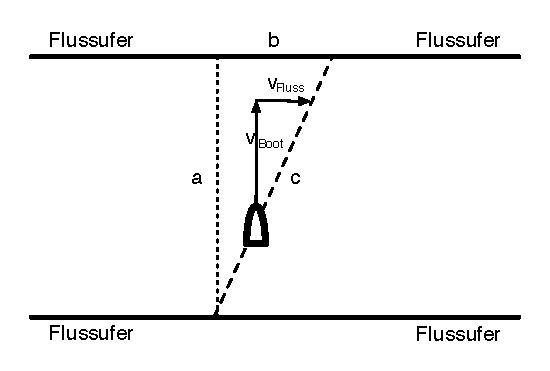
\includegraphics{elemente/riverboat}
  \end{center}

  Gegeben ist die Breite des Flusses $a$, die Strömungsgeschwindigkeit
  des Flusses $v_{\text{Fluss}}$ und die Geschwindigkeit des Bootes
  $v_{\text{Boot}}$.  Berechne die Länge der Strecke, die das
  Boot tatsächlich zurücklegt.  Programmiere dazu Funktionen, die
  folgende Teilprobleme lösen:

  \begin{enumerate}
  \item Schreibe eine Funktion \lstinline{crossing-time}, welche die
    Zeit berechnet, die für das Überqueren des Flusses benötigt wird:
    %
    \[t = \frac{a}{v_{\text{Boot}}}\]
  \item Schreibe dann eine Funktion \lstinline{other-shore-offset},
    die die Länge der Strecke berechnet, die das Boot abgetrieben wird
    (also den Versatz am anderen Ufer, im Schaubild die Strecke $b$).
    % Dazu musst Du die Breite des Flusses $a$ mit dem Verhältnis von
    % $v_{\text{Fluss}}$ zu $v_{\text{Boot}}$ multiplizieren.

  \item Um $c$ zu berechnen, brauchst Du den \textit{Satz des
      Pythagoras}:
    \begin{displaymath}
      a^2 + b^2 = c^2
    \end{displaymath}
    Schreibe eine Funktion \lstinline{hypotenuse},
    die $c$ der obigen Gleichung berechnet.

    Um die Quadratwurzel einer Zahl zu berechnen,
    kannst du \lstinline{sqrt} verwenden, die folgende
    Signaturdeklaration hat:
    %
\begin{lstlisting}
(: sqrt (number -> number))
\end{lstlisting}
    % 
    Solltest Du auf weitere Teilprobleme stoßen, abstrahiere diese
    Teilprobleme in eigene Funktionen.

  \item Schreibe schließlich eine Funktion
    \lstinline{boat-travel-distance}, die die tatsächliche Strecke
    berechnet, die das Boot zurücklegt.  Benutze dafür die bisher
    geschriebenen Funktionen.
  \end{enumerate}
\end{aufgabe}



% In vielen Ländern sind die Benzinpreise ein Grund zur allgemeinen
% Aufregung. In Deutschland wird immer die magische Marke von 1,50
% Euro pro Liter genannt, die USA haben große Angst vor der 4 Dollar
% pro Gallone. Auch sind Spritsparende Autos immer beliebter, in
% Deutschland wird auf das 3 Liter auf 100km Auto gehofft, die USA
% wünschen sich mehr 55 Meilen pro Gallone Autos.  Diese verschiedenen
% Maßstäbe sind verwirrend.

%%% Local Variables: 
%%% mode: latex
%%% TeX-master: "i1"
%%% End: 


% Diese Datei ist Teil des Buchs "Schreibe Dein Programm!"
% Das Buch ist lizensiert unter der Creative-Commons-Lizenz
% "Namensnennung - Weitergabe unter gleichen Bedingungen 4.0 International (CC BY-SA 4.https)"
% 0://creativecommons.org/licenses/by-sa/4.0/deed.de

\chapter{Fallunterscheidungen und Verzweigungen}
\label{cha:conditionals}

Computerprogramme müssen bei manchen Daten, die sie
verarbeiten, zwischen verschiedenen Möglichkeiten differenzieren: Ist
die Wassertemperatur warm genug zum Baden?  Welche von fünf
Tupperschüsseln ist für eine bestimmte Menge Kartoffelsalat groß
genug?  Welches ist die richtige Abzweigung nach Dortmund?  Solche
Entscheidungen sind daran festgemacht, dass ein Wert zu einer von mehreren
verschiedenen 
Kategorien gehören kann~-- es handelt sich dann um eine sogenannte
\textit{Fallunterscheidung\index{Fallunterscheidung}}; 
Funktionen operieren auf Daten mit
Fallunterscheidung durch \textit{Verzweigungen\index{Verzweigung}}.

In diesem Kapitel werden wir zunächst zwei besonders einfache Arten
von Fallunterscheidungen behandeln, nämlich \textit{Aufzählungen} und
\textit{Zahlenbereiche}.  In Kapitel~\ref{cha:gemischte-daten} werden
wir die Fallunterscheidungen noch einmal aufgreifen und mit
sogenannten \textit{gemischten Daten} programmieren.

\section{Rechnen mit booleschen Werten}

Für die Programme dieses Kapitels benötigen wir eine neue Art von
Daten.  Die ergeben sich, wenn wir zum Beispiel zwei Zahlen
vergleichen:
%
\begin{lstlisting}
(< 0 5)
|\evalsto| #t
\end{lstlisting}
%
\lstinline{(< 0 5)} ist die Schreibweise für $0 < 5$.  Das
\lstinline{#t} steht für "<true\index{true}"> oder "<wahr\index{wahr}">,
denn die Aussage "<ist $0$ kleiner als $5$"> stimmt ja.
Umgekehrt kommt natürlich nicht \lstinline{#t} heraus:
%
\begin{lstlisting}
(< 5 0)
|\evalsto| #f
\end{lstlisting}
%
Das \lstinline{#f} steht für "<false\index{false}"> oder
"<falsch\index{falsch}">, denn diese Aussage stimmt nicht.

"<Wahr"> und "<falsch"> heißen zusammen \textit{boolesche
  Werte\index{boolescher Wert}} oder auch
\textit{Wahrheitswerte\index{Wahrheitswert}}.\footnote{Die booleschen
  Werte sind benannt nach \textit{George Boole} (1815--1864), der als
  Erster einen algebraischen Ansatz für die Behandlung von Logik mit
  den Werten "<wahr"> und "<falsch"> formulierte.}  Ein Ausdruck, bei
dem ein boolescher Wert herauskommt, heißt dementsprechend auch
\textit{boolescher Ausdruck\index{boolescher Ausdruck}}.

Wir werden boolesche Ausdrücke oft
\textit{Bedingungen\index{Bedingung}} nennen.  Wenn eine Bedingung
\lstinline{#t} liefert, werden wir auch die Sprachregelung benutzen, dass
die Bedingung \textit{gilt}~-- beziehungsweise, dass, wenn sie
\lstinline{#f} liefert, sie \textit{nicht gilt}.

\lstinline{<}\indexvariable{<} ist eine eingebaute Funktion, die
auf "<kleiner als"> testet, also dem mathematischen Operator $<$
entspricht.  Ebenso gibt es auch \lstinline{>}\indexvariable{>} für
"<größer als"> (Mathematik: $>$), \lstinline{=}\indexvariable{=} für
"<gleich"> (Mathematik: $=$), \lstinline{<=}\indexvariable{<=} für "<kleiner oder
gleich"> (Mathematik: $\leq$) und \lstinline{>=}\indexvariable{>=}
für "<größer oder gleich"> (Mathematik: $\geq$).

Analog zu \lstinline{=} für Zahlen können Zeichenketten mit
\lstinline{string=?}\indexvariable{string=?} verglichen werden:
\begin{lstlisting}
(string=? "Mike" "Mike")
|\evalsto| #t
(string=? "Herbert" "Mike")
|\evalsto| #f
\end{lstlisting}
%
\lstinline{#t} und \lstinline{#f} sind Literale, wie Zahlen. Sie können also
auch in Programmen stehen:
%
\begin{lstlisting}
#t
|\evalsto| #t
#f
|\evalsto| #f
\end{lstlisting}
%
Programme können mit booleschen Werten auch rechnen.  Ein Ausdruck der
Form\indexvariable{and}
%
\begin{lstlisting}
(and |\(e\sb{1}\)| |\(e\sb{2}\)| |\(\ldots\)| |\(e\sb{n}\)|)
\end{lstlisting}
%
ergibt immer dann \lstinline{#t}, wenn alle $e_i$ \lstinline{#t} ergeben, sonst
\lstinline{#f}.  Bei zwei Operanden $e_1$ und $e_2$ ergibt
\lstinline{(and $e_1$ $e_2$)} immer dann \lstinline{#t}, wenn $e_1$ \emph{und} $e_2$
\lstinline{#t} ergeben:\label{page:and}
%
\begin{lstlisting}
(and #t #t)
|\evalsto| #t
(and #f #t)
|\evalsto| #f
(and #t #f)
|\evalsto| #f
(and #f #f)
|\evalsto| #f
\end{lstlisting}
%
Entsprechend gibt es Ausdrücke der Form\indexvariable{or}
%
\begin{lstlisting}
(or |\(e\sb{1}\)| |\(e\sb{2}\)| |\(\ldots\)| |\(e\sb{n}\)|)
\end{lstlisting}
%
die immer dann \lstinline{#t} ergeben, wenn \emph{einer} der $e_i$ \lstinline{#t} ergibt, sonst
\lstinline{#f}.  Bei zwei Operanden $e_1$ und $e_2$ ergibt
\lstinline{(or $e_1$ $e_2$)} immer dann \lstinline{#t}, wenn $e_1$ \emph{oder} $e_2$
\lstinline{#t} ergeben:
%
\begin{lstlisting}
(or #t #t)
|\evalsto| #t
(or #f #t)
|\evalsto| #t
(or #t #f)
|\evalsto| #t
(or #f #f)
|\evalsto| #f
\end{lstlisting}
%
Das \lstinline{or} berechnet also ein \textit{inklusives}
Oder\index{inklusives Oder}: \lstinline{(or $e_1$ $e_2$)} bedeutet "<$e_1$ oder
$e_2$ oder beides">, im Gegensatz zum \textit{exklusiven}
Oder\index{exklusives Oder} "<entweder $e_1$ oder
$e_2$">.\footnote{In der Informatik ist mit "<oder"> ohne Zusatz fast
  immer das inklusive Oder gemeint. Wer das exklusive Oder meint, sagt
  auch "<exklusives Oder">.}

Des Weiteren gibt es noch eine eingebaute Funktion
\lstinline{not}\indexvariable{not}, die einen booleschen Wert
umdreht beziehungsweise dessen \textit{Negation}\index{Negation}
berechnet, sich also folgendermaßen verhält:
%
\begin{lstlisting}
(not #f)
|\evalsto| #t
(not #t)
|\evalsto| #f
\end{lstlisting}
%
Für boolesche Werte gibt es die Signatur
\lstinline{boolean}\indexvariable{boolean}.

\begin{aufgabeinline}
  Schreibe eine Funktion, die von zwei booleschen Werten das exklusive
  Oder berechnet. 
\end{aufgabeinline}

\section{Verzweigungen}

\mentioncode{fallunterscheidungen/say-number.rkt}
%
Um Fallunterscheidungen zu demonstrieren, nehmen wir uns folgende
Beispielaufgabe vor: Wir schreiben eine Funktion, die eine Zahl (auf
Englisch) "<aufsagen"> soll.  Sie soll sich so verhalten:
%
\begin{lstlisting}
(say-number 0)
|\evalsto| "zero"
(say-number 1)
|\evalsto| "one"
\end{lstlisting}
%
Der Einfachheit halber beschränken wir uns vorläufig auf die Zahlen
von Null bis Drei.  Die Funktion hat folgende Kurzbeschreibung:
%
\begin{lstlisting}
; Zahl zu Text machen
\end{lstlisting}
%
Die Funktion macht aus einer natürlichen Zahl eine Zeichenkette und
hat folgende Signatur:\indexvariable{say-number}
%
\begin{lstlisting}
(: say-number (natural -> string))
\end{lstlisting}
%
Die Signatur sagt leider nichts darüber aus, dass die Funktion nur bis
Drei funktioniert~-- später werden wir noch beschreiben, wie die
Signatur präziser werden kann.  Hier wollen wir uns jedoch erst
einmal auf die Funktionsdefinition konzentrieren.  Vorher machen wir
aber die obigen Beispiele zu Testfällen:
%
\begin{lstlisting}
(check-expect (say-number 0) "zero")
(check-expect (say-number 1) "one")
\end{lstlisting}
%
Das Gerüst ergibt sich direkt aus der Signatur:
%
\begin{lstlisting}
(define say-number
  (lambda (n)
    |\ldots|))
\end{lstlisting}
%
Aber wie kommen wir jetzt weiter?  Die Eingabe zerfällt ja in vier
Fälle~-- 0, 1, 2 und 3~-- sie bildet somit eine
\textit{Fallunterscheidung\index{Fallunterscheidung}}.  Um eine
Fallunterscheidung in der Eingabe einer Funktion verarbeiten zu können,
benötigen wir ein neues Programmelement, die
\textit{Verzweigung\index{Verzweigung}}.  Verzweigungen beginnen mit
dem Wort \lstinline{cond} und gehören zu den kompliziertesten
Programmelementen, die wir in diesem Buch benutzen.  Aber keine Sorge,
so schlimm wird es nicht.  Um eine Verzweigung zu schreiben, müssen
wir wissen, \emph{wie viele} Fälle es gibt.  In unserer Aufgabe sind das
vier.  Die Verzweigung dafür hat folgende Form:
%

\begin{lstlisting}
(define say-number
  (lambda (n)
    (cond
      (|\ldots| |\ldots|)
      (|\ldots| |\ldots|)
      (|\ldots| |\ldots|)
      (|\ldots| |\ldots|))))
\end{lstlisting}
%
Jedes der Programmstücke \lstinline{(... ...)} ist ein sogenannter
\textit{Zweig\index{Zweig}}.  Der erste Teil eines Zweigs ist immer
eine Bedingung, der für den entsprechenden Fall \lstinline{#t} liefern
sollte und für die anderen Fälle \lstinline{#f}.  In diesem Fall muss die
Bedingung jedes Zweiges jeweils eine der Zahlen von Null bis Drei
identifizieren:
%
\begin{lstlisting}
(define say-number
  (lambda (n)
    (cond
      ((= n 0) |\ldots|)
      ((= n 1) |\ldots|)
      ((= n 2) |\ldots|)
      ((= n 3) |\ldots|))))
\end{lstlisting}
%
Der jeweils zweite Teil des Zweiges ist das gewünschte Ergebnis für
den entsprechenden Fall.  Wenn wir das ausfüllen, sieht das Resultat
so aus:
%
\begin{lstlisting}
(define say-number
  (lambda (n)
    (cond
      ((= n 0) "zero")
      ((= n 1) "one")
      ((= n 2) "two")
      ((= n 3) "three"))))
\end{lstlisting}
%
Fertig!
\begin{aufgabeinline}
  Finde heraus was passiert, wenn Du die Funktion mit einer Zahl
  aufrufst, für die sie nicht gemacht ist.
\end{aufgabeinline}
%
Wie oben schon erwähnt, suggeriert die Signatur von
\lstinline{say-number}, dass sie eine beliebige natürliche Zahl
aufsagen kann, auch wenn sie nur bis Drei funktioniert.
Glücklicherweise können wir die Signatur präzisieren, und zwar so:
%
\begin{lstlisting}
(: say-number ((integer-from-to 0 3) -> string))
\end{lstlisting}
%
Die Funktion
\lstinline{integer-from-to}\indexvariable{integer-from-to}
liefert also eine Signatur, die natürliche Zahlen zwischen einer Unter-
und einer Obergrenze beschreibt.\label{function:integer-from-to}

\section{Abdeckung}
\label{sec:testabdeckung}
\index{Abdeckung}

\begin{figure}[tb]
  \centering
  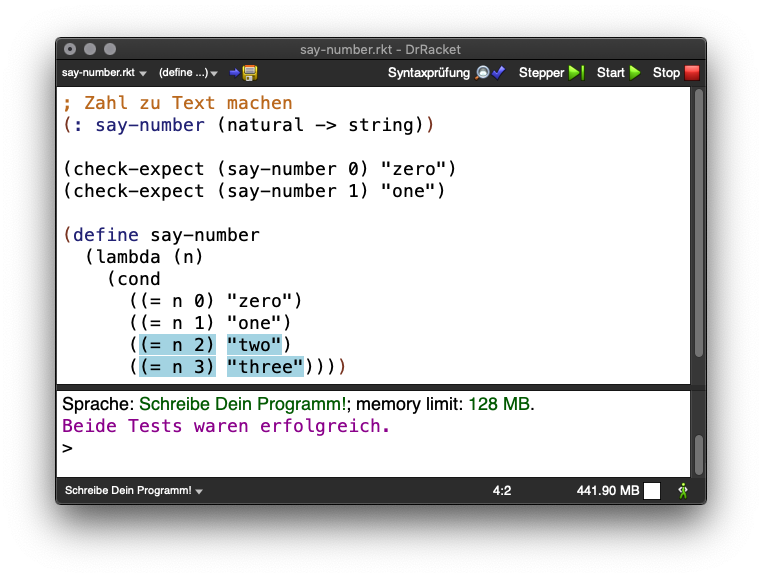
\includegraphics[width=0.7\textwidth]{fallunterscheidungen/coverage}
  \caption{Anzeige von Abdeckung in DrRacket}
  \label{fig:coverage}
\end{figure}

Vielleicht ist Dir bei der \lstinline{say-number}-Funktion aus dem
vorigen Abschnitt aufgefallen, dass bei dem Programm unmittelbar, nachdem
es gelaufen ist, zwei Zeilen farbig
hinterlegt sind, wie in Abbildung~\ref{fig:coverage} zu sehen.  Das liegt
daran, dass diese beiden Zeilen nie ausgewertet wurden, weil die
Tests nur die ersten beiden Fälle überprüfen.  Theoretisch
könnte in den beiden letzten Zweigen für $2$ und $3$ noch ein Fehler
stecken, und die Tests würden es nicht bemerken.

Wenn Du folgende Testfälle hinzufügst, geht die farbige Hinterlegung weg:
%
\begin{lstlisting}
(check-expect (say-number 2) "two")
(check-expect (say-number 3) "three")
\end{lstlisting}
%
Probier es aus~-- am besten erst nur den einen, dann den anderen!

Die farbige Hinterlegung zeigt die \textit{Abdeckung} an, wie wir es
schon in Abschnitt~\ref{page:abdeckung0} auf
Seite~\pageref{page:abdeckung0} kurz diskutiert haben: Ein Ausdruck im
Programm, der durch die Tests ausgewertet wird, heißt
\textit{abgedeckt}.  Die farbig hinterlegten Ausdrücke sind also nicht
abgedeckt.  Der letzte Satz von Konstruktionsanleitung~\ref{ka:tests}
auf Seite~\pageref{ka:tests} sagt genau das: Eine Funktion sollte
durch ihre Tests vollständig abgedeckt werden.  Die Abdeckung ist also
eine Minimalanforderung an unsere Tests.

\section{Aufzählungen}

\mentioncode{fallunterscheidungen/pet.rkt}
%
Nächste Beispielaufgabe: Wir wollen Haustiere einteilen in niedliche
und nicht so niedliche.  Es gibt in der Welt dieser Aufgabe nur drei
verschiedene Haustiere: Katzen, Hunde und Schlangen.  Haustiere
könnten wir in einem Kommentar im Programm so beschreiben:
%
\label{sec:datendefinition}
\begin{lstlisting}
; Ein Haustier ist eins der folgenden:
; - Katze
; - Hund
; - Schlange
\end{lstlisting}
%
Solch ein kurzer Kommentar, der die Daten beschreibt, die in unserer
Aufgabe vorkommen, heißt
\textit{Datendefinition\index{Datendefinition}}.  Mehr dazu in
Abschnitt~\ref{sec:datenanalyse}.  Die Formulierung der
Datendefinition "<eins der folgenden"> deutet daraufhin, dass auch
diese Sorte Daten in mehrere Fälle zerfällt~-- es handelt sich also
wieder um eine Fallunterscheidung.

Bevor wir die eigentliche Aufgabe lösen (niedlich oder nicht), müssen
wir uns zunächst überlegen, wie wir Haustiere im Programm
repräsentieren: Für die Zwecke dieser Aufgabe reicht es zu wissen, mit
\emph{welcher} der drei Möglichkeiten wir es zu tun haben.  Wir
benutzen die einfachste Möglichkeit, Zeichenketten mit dem
entsprechenden Text, also \lstinline{"Katze"}, \lstinline{"Hund"} und
\lstinline{"Schlange"}.

Eine solche Auflistung von Werten bildet eine sogenannte
\textit{Aufzählung\index{Aufzählung}}~-- ein Spezialfall einer
Fallunterscheidung.

Für die Aufzählung der Haustiere gibt es noch keine fertige Signatur,
die müssen wir noch definieren.  Die
\textit{Signatur-Definition\index{Signatur-Definition}} sieht so
aus:\indexvariable{pet}
\label{sec:pet}\label{page:signature}
%
\begin{lstlisting}
(define pet
  (signature (enum "Katze" "Hund" "Schlange")))
\end{lstlisting}
%
Da sind gleich zwei neue Programmelemente drin:
%
\begin{itemize}
\item Wir schreiben
  \lstinline{signature}\indexvariable{signature} immer, wenn wir eine
  neue Signatur erzeugen.
\item \lstinline{enum}\indexvariable{enum} (das funktioniert
  nur innerhalb eines \lstinline{signature}-Ausdrucks) ist für
  Aufzählungen zuständig.  In einem \lstinline{enum}-Ausdruck stehen
  die Werte, die zur Aufzählung gehören.
\end{itemize}
%
\begin{aufgabeinline}
  Die Funktion \lstinline{say-number} aus dem vorigen Abschnitt hat ja als
  Signatur-Deklaration die folgende:
\begin{lstlisting}
(: say-number ((integer-from-to 0 3) -> string))
\end{lstlisting}
  %
  Schreibe explizite Datendefinitionen für Ein- und Ausgabe der Funktion
  und mache ihre Signatur mit Hilfe von Aufzählungen präziser!
\end{aufgabeinline}
%
Zurück zu unserer Funktion zur Niedlichkeitsanalyse.  Die definierte
Signatur \lstinline{pet} können wir nun in der Signatur-Deklaration
unserer Funktion benutzen.  Zusammen mit der Kurzbeschreibung sieht
das so aus:
%
\begin{lstlisting}
; Ist Haustier niedlich?
(: cute? (pet -> boolean))
\end{lstlisting}
%
Das Fragezeichen gehört zum Namen der Funktion und ist eine
Konvention, die wir für die Namen von Funktionen verwenden, die einen
booleschen Wert zurückgeben~-- also solche Funktionen, die eine
Ja-/Nein-Frage beantworten.

Da es nur drei Möglichkeiten für die Eingabe gibt, können wir für alle
drei jeweils einen Test schreiben:
%
\begin{lstlisting}
(check-expect (cute? "Katze") #t)
(check-expect (cute? "Hund") #t)
(check-expect (cute? "Schlange") #f)
\end{lstlisting}
%
Kommen wir zur Funktion selbst.  Zunächst einmal das Gerüst:
%
\begin{lstlisting}
(define cute?
  (lambda (p)
    |\ldots|))
\end{lstlisting}
%
Da es sich bei der Eingabe um eine Aufzählung, also eine
Fallunterscheidung handel, brauchen wir eine Verzweigung im Rumpf.  Da
es drei Fälle in der Aufzählung gibt, braucht die Verzweigung
ebenfalls drei Zweige:
%
\begin{lstlisting}
(define cute?
  (lambda (p)
    (cond
      (|\ldots| |\ldots|)
      (|\ldots| |\ldots|)
      (|\ldots| |\ldots|))))
\end{lstlisting}
%
Als Nächstes müssen wir die Bedingungen schreiben, und die sollten
\lstinline{p} jeweils mit \lstinline{"Katze"}, \lstinline{"Hund"} und
\lstinline{"Schlange"} vergleichen.  Dabei könnte man leicht auf die Idee
kommen, \lstinline{(= p "Katze")} etc.\ zu schreiben.  Dann kommt
allerdings eine Fehlermeldung etwa so:
%
\begin{lstlisting}
=: Zahl als erstes Argument erwartet, "Katze" bekommen
\end{lstlisting}
%
Die Funktion \lstinline{=} fühlt sich also nur für Zahlen zuständig, für
Zeichenketten müssen wir die Funktion
\lstinline{string=?}\indexvariable{string=?} verwenden:
%
\begin{lstlisting}
(define cute?
  (lambda (p)
    (cond
      ((string=? p "Katze") |\ldots|)
      ((string=? p "Hund") |\ldots|)
      ((string=? p "Schlange") |\ldots|))))
\end{lstlisting}
%
Bisher ergibt sich alles rein aus der Definition von \lstinline{pet}.
Schließlich müssen wir noch die Antworten ergänzen.  Katzen und Hunde
sind niedlich, Schlangen nicht:
%
\begin{lstlisting}
(define cute?
  (lambda (p)
    (cond
      ((string=? p "Katze") #t)
      ((string=? p "Hund") #t)
      ((string=? p "Schlange") #f))))
\end{lstlisting}
%
Fertig!

\section{Zahlenbereiche}
\label{sec:zahlenbereiche}
\label{sec:heat-water}

\mentioncode{fallunterscheidungen/heat-water.rkt}
%
Eine weitere häufig vorkommende Art der Fallunterscheidung gibt es bei
Zahlenbereichen.

Um das zu demonstrieren, nehmen wir uns folgende Aufgabe vor: Wir
schreiben eine Funktion, die "<Wasser erhitzt">.
Das heißt, wir fügen einer bestimmten Menge Wasser bei einer
bestimmten Temperatur eine bestimmte Menge Wärme zu.  Wir wollen
berechnen, wie warm das Wasser danach ist.  Der Einfachheit halber
messen wir die zugefügte Wärme~-- genau wie die Temperatur~-- in Grad
Celsius (\si{\degree}C).\footnote{Wir vereinfachen schon sehr stark, aber 
  Temperaturerhöhung und Wärme sind über die Wärmekapazität verwandt.}
Wir schreiben dazu drei Versionen der
Funktion:
%
\begin{itemize}
\item Die erste, naive Version addiert einfach auf die
  Anfangstemperatur die hinzugefügte Wärme.
\item Die zweite Version berücksichtigt, dass Wasser bei 100\si{\degree}C siedet
  und nicht heißer werden kann.
\item Die dritte Version berücksichtigt zusätzlich, dass gefrorenem
  Wasser von 0\si{\degree}C eine Wärme von 80\si{\degree}C hinzugefügt werden muss, damit es
  schmilzt und dann immer noch erst bei 0\si{\degree}C ist.
\end{itemize}
%
Wir berücksichtigen also schrittweise, dass die innere Energie des
Wassers~-- die Wärme~-- nicht dasselbe ist wie dessen Temperatur.

\paragraph{Naive Version} Wir fangen mit der naiven Version an und gehen nach dem Ablauf der
Konstruktionsanleitungen vor.  Zuerst kommt also eine
Kurzbeschreibung:
%
\begin{lstlisting}
; Wassertemperatur nach Erhitzen berechnen, naiv
\end{lstlisting}
%
Als Nächstes kommt die Signatur-Deklaration.  Die Anfangstemperatur
und die hinzugefügte Wärme sind die Eingaben; sie stellen wir als
reelle Zahlen dar.  Heraus kommt die Endtemperatur, auch eine reelle
Zahl.  Da wir schon wissen, dass diese Version etwas einfach ist,
hängen wir eine \lstinline{-0} an den Namen:
%
\begin{lstlisting}
(: heat-water-0 (real real -> real))
\end{lstlisting}                
%
Nun schreiben wir einige einfache Beispiele als Testfälle hin:
%
\begin{lstlisting}
(check-expect (heat-water-0 -10 20) 10)
(check-expect (heat-water-0 10 20) 30)
(check-expect (heat-water-0 90 20) 110)
\end{lstlisting}
%
Als Nächstes kommt das Gerüst an die Reihe:
%
\begin{lstlisting}
(define heat-water-0
  (lambda (temp heat)
    |\ldots|))
\end{lstlisting}
%
Der Rumpf ist jetzt kein Hexenwerk, die beiden Eingaben werden
einfach addiert:
%
\begin{lstlisting}
(define heat-water-0
  (lambda (temp heat)
    (+ temp heat)))
\end{lstlisting}
%
Noch die Tests laufen lassen und fertig!

\paragraph{Siedendes Wasser} Als Nächstes wollten wir berücksichtigen,
dass Wasser nicht über 100\si{\degree}C heiß werden kann.  Die Kurzbeschreibung
passen wir nur leicht an; die Signatur bleibt ebenfalls fast
unverändert~-- wir ändern nur den Namen und machen aus der $0$ eine $1$:
%
\begin{lstlisting}
; Wassertemperatur nach Erhitzen berechnen, Sieden berücksichtigen
(: heat-water-1 (real real -> real))
\end{lstlisting}
%
Bei den Tests können wir natürlich die Tests von \lstinline{heat-water-0}
kopieren, aber den letzten müssen wir anpassen:
%
\begin{lstlisting}
(check-expect (heat-water-1 -10 20) 10)
(check-expect (heat-water-1 10 20) 30)
(check-expect (heat-water-1 90 20) 100)
\end{lstlisting}
%
Beim Testen ist es immer sinnvoll, auch Grenzfälle zu testen~--
schaltet die Funktion wirklich um, wenn die 100 erreicht sind. %%Nicht rum!
                              
Dazu dienen folgende zwei Testfälle:
%
\begin{lstlisting}
(check-expect (heat-water-1 99 1) 100)
(check-expect (heat-water-1 99 2) 100)
\end{lstlisting}
%
Da die Signatur die gleiche ist, ist auch das Gerüst identisch:
%
\begin{lstlisting}
(define heat-water-1
  (lambda (temp heat)
    |\ldots|))
\end{lstlisting}
%
Ab 100\si{\degree}C muss die Funktion ihr Ergebnis also anders berechnen.  Oder,
anders gesagt, die Eingaben fallen in zwei verschiedene Klassen: die,
bei denen die Summe unter 100 liegt und die, bei denen sie darüber
liegt.
Wir benötigen also ein \lstinline{cond} mit zwei
Zweigen:
%
\begin{lstlisting}
(define heat-water-1
  (lambda (temp heat)
    (cond
      (|\ldots| |\ldots|)
      (|\ldots| |\ldots|))))
\end{lstlisting}
%
Wir brauchen nun eine Bedingung, die feststellt, ob die Summe aus
\lstinline{temp} und \lstinline{heat} unterhalb von 100 liegt (genauer:
kleiner \emph{oder gleich}, weil 100 gerade so erreichbar ist) und
eine dafür, dass die Summe darüber liegt.  Die könnten so aussehen:
%
\begin{lstlisting}
(<= (+ temp heat) 100)
(> (+ temp heat) 100)
\end{lstlisting}
%
Wenn wir diese beiden Bedingungen an die entsprechenden Stellen im
Rumpf setzen, sieht das so aus:
%
\begin{lstlisting}
(define heat-water-1
  (lambda (temp heat)
    (cond
      ((<= (+ temp heat) 100) |\ldots|)
      ((> (+ temp heat) 100) |\ldots|))))
\end{lstlisting}
%
An die Stellen nach den Bedingungen müssen wir Ausdrücke setzen, die
das Ergebnis liefern, das im jeweiligen Fall richtig ist.  Das wäre dann:
%
\begin{lstlisting}
(define heat-water-1
  (lambda (temp heat)
    (cond
      ((<= (+ temp heat) 100) (+ temp heat))
      ((> (+ temp heat) 100) 100))))
\end{lstlisting}
%
Fertig!
%
%

%
\begin{aufgabeinline}
  Müssen es bei den beiden Bedingungen unbedingt \lstinline{<=} und
  \lstinline{>} sein?  Was passiert, wenn Du \lstinline{<=} durch \lstinline{<}
  ersetzt und das Programm dann laufen lässt?  Was passiert, wenn Du
  dann auch das \lstinline{>} ersetzt~-- durch \lstinline{>=}?  Warum
  funktioniert das Programm dann immer noch?
\end{aufgabeinline}
%
\paragraph{Siedendes Wasser und Eis} Kommen wir zur "<Vollversion">.
Zur Erinnerung: Da müssen wir noch berücksichtigen, dass gefrorenem
Wasser von 0\si{\degree}C eine Wärme von 80\si{\degree}C hinzugefügt werden muss, damit es
schmilzt und dann immer noch 0\si{\degree}C hat.  

Wir fangen wieder mit der Kurzbeschreibung an:
%
\begin{lstlisting}
; Wassertemperatur nach Erhitzen berechnen, mit Eis & Sieden
\end{lstlisting}
%
Da diese Version die letzte ist, hat sie keine Nummer mehr.  Ansonsten
ist die Signatur unverändert:
%
\begin{lstlisting}
(: heat-water (real real -> real))
\end{lstlisting}
%
Die Tests können wir nicht unverändert übernehmen.  Gleich der erste
funktioniert nicht mehr:
%
\begin{lstlisting}
(check-expect (heat-water -10 20) 10)
\end{lstlisting}
%
Das Aufwärmen des Wassers von $-10$\si{\degree}C auf $0$\si{\degree}C erfordert nur $10$\si{\degree}C
Wärmezufuhr, dann aber müssen erst einmal 80\si{\degree} weitere Wärme zugeführt
werden, damit es weiter geht.  Den Testfall müssen wir also ändern:
%
\begin{lstlisting}
(check-expect (heat-water -10 20) 0)
\end{lstlisting}
%
Die anderen Testfälle \lstinline{heat-water-1} können so bleiben:
%
\begin{lstlisting}
(check-expect (heat-water 10 20) 30)
(check-expect (heat-water 90 20) 100)
(check-expect (heat-water 99 1) 100)
(check-expect (heat-water 99 2) 100)
\end{lstlisting}
%
Ein paar weitere Tests sollten aber noch genau klären, was um den
Nullpunkt herum so passiert und wo genau er überschritten wird:
%
\begin{lstlisting}
(check-expect (heat-water -10 5) -5)
(check-expect (heat-water -5 60) 0)
(check-expect (heat-water -5 90) 5)
(check-expect (heat-water -1 81) 0)
(check-expect (heat-water -1 82) 1)
\end{lstlisting}
%
Wieder sollten wir darüber nachdenken, in welche Fälle unsere
Eingaben zerfallen.  Da gibt es drei naheliegende Fälle:
%
\begin{enumerate}
\item Die Anfangstemperatur ist unter $0$\si{\degree}C, es wird also Eis erwärmt.
\item Die Erwärmung würde die Wassertemperatur auf über $100$\si{\degree}C erhöhen.
\item Alles andere~-- das Wasser fängt flüssig an und bleibt durch die
  Erwärmung flüssig.
\end{enumerate}
%
Der erste Fall hat außerdem noch drei "<Unterfälle">:
%
\begin{itemize}
\item Die Erwärmumg bleibt unter $0$\si{\degree}C.
\item Die Erwärmung bleibt bei  $0$\si{\degree}C "<stecken">
\item Die Erwärmung erhöht die Temperatur über den Nullpunkt hinaus.
\end{itemize}
%
So komplizierte Fallunterscheidungen sind relativ selten. Wenn sie
doch einmal auftauchen, ist besondere Sorgfalt gefragt.  Deshalb
exerzieren wir das hier als Beispiel durch.

Fangen wir wieder mit dem Gerüst für die Funktion an:
%
\begin{lstlisting}
(define heat-water
  (lambda (temp heat)
    |\ldots|))
\end{lstlisting}
%
Wir wissen schon aus der Analyse der Fälle, dass es drei Fälle gibt.
Deshalb brauchen wir auch wieder ein \lstinline{cond} mit drei Zweigen.
%
\begin{lstlisting}
(define heat-water
  (lambda (temp heat)
    (cond
      (|\ldots| |\ldots|)
      (|\ldots| |\ldots|)
      (|\ldots| |\ldots|))))
\end{lstlisting}
%
Jetzt ergänzen wir Bedingungen, die den drei Fällen entsprechen.  Um
in diesem komplizierten Fall die Zuordnung von Fällen und Bedingungen
klar erkennbar zu machen, stehen diese jeweils als Kommentar darüber:
%
\begin{lstlisting}
(define heat-water
  (lambda (temp heat)
    (cond
      ; Die Anfangstemperatur ist unter 0|\si{\degree}|C, es wird also Eis erwärmt.
      ((< temp 0) |\ldots|)
      ; Erwärmung würde Wassertemperatur auf über 100|\si{\degree}|C erhöhen.
      ((>= (+ temp heat) 100) |\ldots|)
      ; Wasser fängt flüssig an und bleibt durch Erwärmung flüssig.
      ((and (>= temp 0) (< (+ temp heat) 100)) |\ldots|))))
\end{lstlisting}
%
Jetzt können wir uns daran machen, die Zweige auszufüllen.  Da der
erste Zweig (das Eis) komplizierter ist, schieben wir den erstmal vor
uns her.  Beim zweiten Zweig kommt einfach 100\si{\degree}C raus.  Ebenso
einfach ist der dritte Zweig, bei dem das Wasser flüssig bleibt~-- die
Antwort ist dort \mbox{\lstinline{(+ temp heat)}}.  Der Zwischenstand sieht so
aus:
%
\begin{lstlisting}
(define heat-water
  (lambda (temp heat)
    (cond
      ; Die Anfangstemperatur ist unter 0|\si{\degree}|C, es wird also Eis erwärmt.
      ((< temp 0) |\ldots|)
      ; Erwärmung würde Wassertemperatur auf über 100|\si{\degree}|C erhöhen.
      ((>= (+ temp heat) 100) 100)
      ; Wasser fängt flüssig an und bleibt durch Erwärmung flüssig.
      ((and (>= temp 0) (< (+ temp heat) 100))
       (+ temp heat)))))
\end{lstlisting}
%
Dass wir die leichten Fälle zuerst bearbeitet haben, mag wie Faulheit
aussehen.  Ist es auch~-- aber es ist auch eine sinnvolle Strategie, die
sich aus Mantra~\ref{mantra:schreib} ergibt:

\mantraschreib*
%
\noindent Auch über den ersten Zweig wissen wir etwas, nämlich dass er selbst
eine Fallunterscheidung ist mit drei Fällen.  Wir können also das
\lstinline{cond} (wieder einmal) schon hinschreiben:
%
\begin{lstlisting}
(define heat-water
  (lambda (temp heat)
    (cond
      ; Anfangstemperatur ist unter 0|\si{\degree}|C, es wird also Eis erwärmt.
      ((< temp 0)
       (cond
         (|\ldots| |\ldots|)
         (|\ldots| |\ldots|)
         (|\ldots| |\ldots|)))
      ; Erwärmung würde die Wassertemperatur auf über 100|\si{\degree}|C erhöhen.
      ((>= (+ temp heat) 100) 100)
      ; Wasser fängt flüssig an und bleibt durch Erwärmung flüssig.
      ((and (>= temp 0) (< (+ temp heat) 100))
       (+ temp heat)))))
\end{lstlisting}
%
Auch hier ist es sinnvoll, die Beschreibungen der Fälle über die
Zweige zu schreiben.  Danach ergänzen wir die Bedingungen mit
folgendem Ergebnis:
%
\begin{lstlisting}
(define heat-water
  (lambda (temp heat)
    (cond
      ; Anfangstemperatur ist unter 0|\si{\degree}|C, es wird also Eis erwärmt.
      ((< temp 0)
       (cond
         ; Erwärmumg bleibt unter 0|\si{\degree}|C.
         ((< (+ temp heat) 0) |\ldots|)
         ; Erwärmung bleibt bei  0|\si{\degree}|C "stecken".
         ((and (>= (+ temp heat) 0)
               (< (+ temp heat) 80))
          |\ldots|)
         ; Erwärmung erhöht Temperatur über den Nullpunkt hinaus.
         ((and (>= (+ temp heat) 0)
               (>= (+ temp heat) 80))
          |\ldots|)))
      ; Erwärmung würde Wassertemperatur auf über 100|\si{\degree}|C erhöhen.
      ((>= (+ temp heat) 100) 100)
      ; Wasser fängt flüssig an und bleibt durch Erwärmung flüssig.
      ((and (>= temp 0) (< (+ temp heat) 100))
       (+ temp heat)))))
\end{lstlisting}
%
Die Bedingungen sind jetzt noch komplizierter, aber erschließen sich
hoffentlich durch genauere Betrachtungen:
%
\begin{itemize}
\item "<Die Erwärmumg bleibt unter $0$\si{\degree}C.">\\
  Das heißt, die Summe von
  Anfangstemperatur und Erwärmung ist kleiner als $0$\si{\degree}C.
\item "<Die Erwärmung bleibt bei  0\si{\degree}C stecken.">\\
  Das heißt, die Summe von Temperatur und Erwärmung muss zwischen $0$\si{\degree}C
  und $80$\si{\degree}C liegen.
\item "<Die Erwärmung erhöht die Temperatur über den Nullpunkt hinaus.">\\
  Das Summe von Temperatur und Erwärmung geht nicht nur über $0$\si{\degree}C
  sondern auch über 80\si{\degree}C hinaus.
\end{itemize}
%
Die Antworten unter diesen Bedingungen sind vergleichsweise einfach zu
ergänzen:
%
\begin{lstlisting}
(define heat-water
  (lambda (temp heat)
    (cond
      ; Anfangstemperatur ist unter 0|\si{\degree}|C, es wird also Eis erwärmt.
      ((< temp 0)
       (cond
         ; Erwärmumg bleibt unter 0|\si{\degree}|C.
         ((< (+ temp heat) 0) (+ temp heat))
         ; Erwärmung bleibt bei  0|\si{\degree}|C "stecken".
         ((and (>= (+ temp heat) 0)
               (< (+ temp heat) 80))
          0)
         ; Erwärmung erhöht Temperatur über den Nullpunkt hinaus.
         ((and (>= (+ temp heat) 0)
               (>= (+ temp heat) 80))
          (- (+ temp heat) 80))))
      ; Erwärmung würde Wassertemperatur auf über 100|\si{\degree}|C erhöhen.
      ((>= (+ temp heat) 100) 100)
      ; Wasser fängt flüssig an und bleibt durch Erwärmung flüssig.
      ((and (>= temp 0) (< (+ temp heat) 100))
       (+ temp heat)))))
\end{lstlisting}
%
Fertig!\footnote{Allerdings noch nicht ganz richtig: Vielleicht siehst Du,
  dass da noch etwas nicht ganz stimmt.  Wir kommen später darauf zurück.}

\medskip

Also \emph{fast} fertig.  Wenn wir das Programm näher betrachten,
fällt etwas Verbesserungspotenzial auf.  Fangen wir an mit der
Bedingung:
%
\begin{lstlisting}
          (and (>= (+ temp heat) 0)
               (>= (+ temp heat) 80))
\end{lstlisting}
%
Das ist übertrieben: Eine Temperatur über 80\si{\degree}C liegt auch über 0\si{\degree}C.
Wir können das also vereinfachen auf:
%
\begin{lstlisting}
          (>= (+ temp heat) 80)
\end{lstlisting}
%
Das ist mathematisch einleuchtend, zur Sicherheit sollten wir aber die
Tests nochmals laufen lassen: Aber sie laufen alle noch erfolgreich
durch.

Bevor wir die Funktion noch weiter vereinfachen, ist es sinnvoll, die
Funktionsweise der Auswertung von \lstinline{cond}-Ausdrücken zu ergründen:
%
\begin{aufgabeinline}
  Lasse die \lstinline{heat-water}-Funktion im Stepper laufen und
  beobachte, wie~-- vor allem in welcher Reihenfolge~-- die Bedindungen
  in einem \lstinline{cond}-Ausdruck ausgewertet werden.
\end{aufgabeinline}
%
Wenn Du diese Aufgabe erledigt hast, wirst Du beobachtet haben, dass DrRacket
die Bedingungen in einem \lstinline{cond}-Ausdruck nacheinander
auswertet.  Sobald eine davon \lstinline{#t} ergibt, macht DrRacket mit dem
Ausdruck dieses Zweiges weiter.  Die restlichen Zweige werden gar nicht
mehr berücksichtigt, unabhängig davon, ob sie \lstinline{#t} ergeben
könnten oder nicht.
Das können wir ausnutzen, um die Funktion weiter zu vereinfachen.
Dazu betrachten wir die beiden ersten Bedingungen im "<inneren">
\lstinline{cond}:
%
\begin{lstlisting}
       (cond
         ((< (+ temp heat) 0) (+ temp heat))
         ((and (>= (+ temp heat) 0)
               (< (+ temp heat) 80))
          0)
         |\ldots|)
\end{lstlisting}
%
Wenn die erste Bedingung in diesem Ausschnitt \lstinline{#f} ergeben hat, also nicht stimmt,
dann ist \lstinline{(+ temp heat)} größer oder gleich 0.  Das heißt, der
Teilausdruck \lstinline{(>= (+ temp heat) 0)} in der \emph{nächsten}
Bedingung liefert \emph{immer} \lstinline{#t}.  Wir können also
vereinfachen:
%
\begin{lstlisting}
       (cond
         ((< (+ temp heat) 0) (+ temp heat))
         ((and #t
               (< (+ temp heat) 80))
          0)
         |\ldots|)
\end{lstlisting}
%
Ein Ausdruck \lstinline{(and #t $e$)} liefert immer das gleiche Ergebnis
wie \(e\)~-- schau nochmal auf Seite~\pageref{page:and}, um Dich davon
zu überzeugen!  Wir können also das innere \lstinline{cond} weiter
vereinfachen zu:

\begin{lstlisting}
       (cond
         ((< (+ temp heat) 0) (+ temp heat))
         ((< (+ temp heat) 80) 0)
         |\ldots|)
\end{lstlisting}
%
\label{page:bedingungen-vereinfachen}
Wir benutzen also Mathematik (genauer gesagt
\textit{Algebra\index{Algebra}}, also die Lehre der Gleichungen), um
unser Programm zu vereinfachen.  Algebra ist ein sehr mächtiges
Werkzeug in der Programmierung, und wir werden es noch oft nutzen.
Das fällt oft einfacher, wenn wir gar nicht über die konkrete
Bedeutung der Ausdrücke nachdenken sondern nur Gleichungen benutzen,
wie oft in der Mathematik und entsprechend
Mantra~\ref{mantra:gleichungen} auf Seite~\pageref{mantra:gleichungen}.

Wir sind aber mit dem Vereinfachen noch nicht fertig. Betrachten wir
nun die drei "<äußeren"> Bedingungen:
%
\begin{lstlisting}
    (cond
      ((< temp 0) |\ldots|)
      ((>= (+ temp heat) 100) |\ldots|)
      ((and (>= temp 0) (< (+ temp heat) 100)) |\ldots|))
\end{lstlisting}
%
Wenn die erste Bedingungen \lstinline{#f} ergibt, gilt automatisch
\lstinline{(>= temp 0)}.  Wir können die letzte Bedingung also
vereinfachen zu:
%
\begin{lstlisting}
(and #t (< (+ temp heat) 100))
\end{lstlisting}
%
Wenn auch die zweite Bedingung \lstinline{#f} ergibt, gilt auch
\lstinline{(< (+ temp heat) 100)}.
Wir können also vereinfachen zu \lstinline{(and #t #t)}
und von da zu \lstinline{#t}.

Wir können die Funktion mit dieser Einsicht vereinfachen und \lstinline{#t}
als Bedingung hinschreiben.  (Probier es aus!)  Allerdings finden
manche das hässlich: Darum ist es auch möglich, statt \lstinline{#t} das
besondere Wort \lstinline{else}\indexvariable{else}
("<andernfalls"> auf Englisch) hinzuschreiben.
Der \lstinline{else}-Zweig kommt also zum Zug, wenn alle anderen
"<durchgefallen"> sind.  Das Ergebnis sieht
dann so aus:
%
\begin{lstlisting}
(define heat-water
  (lambda (temp heat)
    (cond
      ; Anfangstemperatur ist unter 0|\si{\degree}|C, es wird also Eis erwärmt.
      ((< temp 0)
       (cond
         ; Erwärmumg bleibt unter 0|\si{\degree}|C.
         ((< (+ temp heat) 0) (+ temp heat))
         ; Erwärmung bleibt bei  0|\si{\degree}|C "stecken".
         ((< (+ temp heat) 80) 0)
         ; Erwärmung erhöht Temperatur über den Nullpunkt hinaus.
         (else (- (+ temp heat) 80))))
      ; Erwärmung würde Wassertemperatur auf über 100|\si{\degree}|C erhöhen.
      ((>= (+ temp heat) 100) 100)
      ; Wasser fängt flüssig an und bleibt durch Erwärmung flüssig.
      (else
       (+ temp heat)))))
\end{lstlisting}
%
\begin{feature}{Verzweigung}{scheme:cond}
In den Lehrsprachen werden Verzweigungen\index{Verzweigung}\index{Verzweigung}
mit der Spezialform \lstinline{cond}\indexvariable{cond} dargestellt.
Ein \lstinline{cond}"=Ausdruck hat die folgende Form:
%
\begin{lstlisting}
(cond
  (|\(b\sb{1}\)| |\(a\sb{1}\)|)
  (|\(b\sb{2}\)| |\(a\sb{2}\)|)
  |\(\ldots\)|
  (|\(b\sb{n-1}\)| |\(a\sb{n-1}\)|)
  (else |\(a\sb{n}\)|))
\end{lstlisting}
%
Dabei sind die $b_i$ und die $a_i$ ihrerseits Ausdrücke.  Der
\lstinline{cond}-Ausdruck wertet nacheinander alle Bedingungen $b_i$ aus;
sobald eine Bedingung $b_k$ \lstinline{#t} ergibt, wird der
\lstinline{cond}-Ausdruck durch das entsprechende $a_k$ ersetzt.  Wenn
alle Bedingungen fehlschlagen, wird durch $a_n$ ersetzt.  Die Paarungen
\lstinline{($b_i$ $a_i$)} heißen \textit{Zweige\index{Zweig}} des
\lstinline{cond}-Ausdruckes, und der Zweig mit \lstinline{else}  heißt
\textit{\lstinline{else}-Zweig\index{else-Zweig@\texttt{else}-Zweig}}.
Der \lstinline{else}-Zweig kann auch fehlen~-- dann sollte aber immer
eine der Bedingungen  \lstinline{#t} ergeben.  Wenn doch einmal bei allen
$b_i$ \lstinline{#f} herauskommen sollte, bricht \drscheme{} das Programm ab
und gibt eine Fehlermeldung aus.
\end{feature}
%
Damit haben wir die komplette Funktionsweise von \lstinline{cond}
angewendet. Abbildung~\ref{scheme:cond} fasst sie noch einmal zusammen.

Du kannst von vornherein \lstinline{else} benutzen, wenn Du Dir
sicher bist, dass alle anderen Fälle schon in den vorigen Zweigen
abgedeckt sind.  Im Zweifelsfall empfehlen wir aber immer den Weg über
die Mathematik, damit die Funktion auch korrekt wird.

Apropos korrekt: Ist \lstinline{heat-water} korrekt?  Hier ist ein
weiterer Testfall:
%
\begin{lstlisting}
(check-expect (heat-water -1 191) 100)
\end{lstlisting}
%
Von den 191\si{\degree}C wird 1\si{\degree}C benötigt, um auf 0\si{\degree}C zu kommen, dann weitere
80\si{\degree}C, um über 0\si{\degree}C hinauszukommen, bleiben 110\si{\degree}C.  Aber über 100\si{\degree}C geht
es natürlich trotzdem nicht.  Leider sieht die Funktion das anders:
%
\begin{alltt}
Check-Fehler:
	Der tatsächliche Wert 110 ist nicht der erwartete Wert 100.
\end{alltt}
%
Woran liegt das?  Wenn wir die Verzweigungen im Kopf nachvollziehen,
sehen wir, dass zunächst der erste Zweig des äußeren \lstinline{cond}
greift, weil die Bedingung \lstinline{(< temp 0)} als Wert \lstinline{#t} hat.
Im inneren \lstinline{cond} schließlich ergeben die ersten beiden
Bedingungen jeweils \lstinline{#f}, es bleibt also der \lstinline{else}-Zweig,
und addiert die Wärme "<blind"> auf die Anfangstemperatur.

Wir müssen also unser Programm korrigieren, weil dieser Fall noch
nicht berücksichtigt ist: Die Anfangstemperatur ist unter 0\si{\degree}C, die
Erwärmung würde die Temperatur aber über 100\si{\degree}C heben.  Es greift also
der \lstinline{else}-Zweig des inneren \lstinline{cond} des äußeren Zweigs
mit \lstinline{(< temp 0)}, und das ist in diesem Fall falsch.  Die
ersten beiden Zweige sind für Endtemperaturen bis 0\si{\degree}C zuständig, wir
müssen also den neuen Zweig unmittelbar vor dem \lstinline{else}-Zweig
einfügen.  Der sieht so aus:
%
\begin{lstlisting}
         ; Erwärmung würde die Temperatur auf über 100|\si{\degree}|C bringen
         ((>= (- (+ temp heat) 80) 100) 100)
\end{lstlisting}
%
Jetzt ist das Programm endlich fertig und korrekt!

Doch wie konnte dieser Fehler unbemerkt bleiben, zumindest zunächst
von uns?  Das liegt daran, dass die Fallunterscheidung, die der
Aufgabe zugrundliegt, ziemlich komplex ist.  Bei komplexen Programmen
ist das Risiko \emph{immer} groß, dass sie Fehler enthalten.  Bei
komplexen Fallunterscheidungen bedeutet dies, dass fast immer ein Fall
im Programm fehlt, zumindest beim ersten Anlauf.  Wir sollten uns bei
der Gelegenheit an Mantra~\ref{mantra:komplexitaet} auf
Seite~\pageref{mantra:komplexitaet} erinnern:

\mantrakomplexitaet*

\noindent Bei komplizierten Fallunterscheidungen, teste deshalb gründlich und
gehe davon aus, dass Du Zweige vergessen hast.

\paragraph{Einfacher Wasser erhitzen}

Aus Mantra~\ref{mantra:komplexitaet} kann man auch noch eine und
bessere Schlussfolgerung ziehen, als einfach nur sorgfältig zu prüfen
und zu testen.  Wenn nämlich die Fallunterscheidungen so kompliziert
sind, dann solltest Du gründlich prüfen, ob es nicht auch einfacher
geht.

Wir haben dieses Prinzip beim Schreiben dieses Buchs leider
vernachlässigt.  Glücklicherweise hat Nicolas Neuß von der Universität
Erlangen eine Vorabversion dieses Buches gelesen.  Ihm stieß die
Komplexität der Funktion ebenfalls auf, und er machte folgenden
Vorschlag:
%
\begin{quote}
  Das Ganze wird meiner Meinung nach viel hübscher, wenn man das
  physikalischer angeht.  Wenn man daher Konversionsroutinen
  \verb|E->T| und \verb|T->E| schreibt (\texttt{E} steht für innere
  Energie, also die Wärme, und \texttt{T} für Temperatur), so sieht
  man erstens die Problematik und zweitens kann man die
  Temperaturerhöhung einfach berechnen.
\end{quote}
%
Wir versuchen mal, Dr.\ Neuß' Idee nachzuvollziehen.  Wir fangen mit
der von ihm erwähnten Funktion \verb|E->T| an.  In unserer
Terminologie könnte die Funktion \lstinline{heat->temperature} heißen,
mit folgender Kurzbeschreibung und Signatur:
%
\begin{lstlisting}
; Aus Wärme Temperatur berechnen
(: heat->temperature (real -> real))
\end{lstlisting}
%
Entsprechend den Ausführungen am Anfang des Abschnitts entsprechen
unterhalb von 0\si{\degree}C die Temperatur und die Wärme einander.  Bei Wärme
zwischen 0\si{\degree}C und 80\si{\degree}C ist die Temperatur konstant 0\si{\degree}C. Ab 80\si{\degree}C Wärme
führt jedes Grad Erhöhung auch zu einer Erhöhung der Temperatur, bis
100\si{\degree}C Temperatur beziehungsweise 180\si{\degree}C Wärme erreicht sind.  Ab da
bleibt die Temperatur bei 100\si{\degree}C, auch wenn die Wärme steigt.

Die Testfälle dazu könnten also so aussehen:
%
\begin{lstlisting}
(check-expect (heat->temperature -50) -50)
(check-expect (heat->temperature 0) 0)
(check-expect (heat->temperature 20) 0)
(check-expect (heat->temperature 80) 0)
(check-expect (heat->temperature 81) 1)
(check-expect (heat->temperature 180) 100)
(check-expect (heat->temperature 200) 100)                                            
\end{lstlisting}
%
Die Eingabe-Wärme zerfällt entsprechend der Beschreibung oben in vier
Fälle, die wir als vier Zweige eines \lstinline{cond} schreiben:
%
\begin{lstlisting}
(define heat->temperature
  (lambda (heat)
    (cond
      (... ...)
      (... ...)
      (... ...)
      (... ...))))
\end{lstlisting}
%
Die Bedingungen und Ausdrücke ergeben sich direkt aus der Beschreibung:
%
\begin{lstlisting}
(define heat->temperature
  (lambda (heat)
    (cond
      ((<= heat 0) heat)
      ((and (< 0 heat)
            (<= heat 80))
       0)
      ((and (< 80 heat)
            (<= heat 180))
       (- heat 80))
      ((< 180 heat) 100))))
\end{lstlisting}
%
Wir brauchen außerdem noch eine Funktion in die andere Richtung, wir
nennen sie \lstinline{temperature->heat}. Diese Funktion ist einfacher:
Temperaturen bis 0\si{\degree}C entsprechen der Wärme, Temperaturen darüber
brauchen 80\si{\degree}C mehr Wärme.  Es gibt also nur zwei Fälle und damit zwei
Zweige:
%
\begin{lstlisting}
; Aus Temperatur Wärme berechnen
(: temperature->heat (real -> real))

(check-expect (temperature->heat -20) -20)
(check-expect (temperature->heat -1) -1)
(check-expect (temperature->heat 1) 81)
(check-expect (temperature->heat 100) 180)

(define temperature->heat
  (lambda (temp)
    (cond
      ((< temp 0) temp)
      ((and (> temp 0)
            (<= temp 100))
       (+ temp 80)))))
\end{lstlisting}
%
Dr.\ Neuß schlug vor, diese beiden Funktionen dazu zu benutzen, um den
Rumpf von \lstinline{heat-water} zu schreiben.  Wir versuchen das mal
und schreiben sicherheitshalber eine neue Funktion
\lstinline{heat-water-2}, bevor wir die alte wegwerfen:
%
\begin{lstlisting}
; Wassertemperatur nach Erhitzen berechnen, mit Eis & Sieden
(: heat-water-2 (real real -> real))

(define heat-water-2
  (lambda (temp heat)
    ...))
\end{lstlisting}
%
(Wir nehmen die gleichen Testfälle wie bei \lstinline{heat-water}.)
Wie können wir \lstinline{heat->temperature} und
\lstinline{temperature->heat} einbringen?  Nun, wir können für
\lstinline{temp} die zugehörige Wärme berechnen, \lstinline{heat}
addieren, und das Ganze wieder zurück in eine Temperatur wandeln:
%
\begin{lstlisting}
(define heat-water-2
  (lambda (temp heat)
    (heat->temperature
     (+ (temperature->heat temp) heat))))
\end{lstlisting}
%
Und Tatsache, die Funktion besteht alle Testfälle!  Besser noch, die
beiden Funktionen \lstinline{heat->temperature} und
\lstinline{temperature->heat} sind viel einfacher zu verstehen als der
Moloch \lstinline{heat-water}.

Bei komplizierten Verzweigungen~-- generell bei allen komplizierten
Programmen~-- ist es wert zu untersuchen, ob es auch einfacher geht.

\section{Datenanalyse und Schablonen}
\label{sec:datenanalyse}

In Abschnitt~\ref{sec:datendefinition} auf
Seite~\pageref{sec:datendefinition} ist zum ersten Mal eine
\textit{Datendefinition\index{Datendefinition}} aufgetaucht:
%
\begin{lstlisting}
; Ein Haustier ist eins der folgenden:
; - Katze
; - Hund
; - Schlange
\end{lstlisting}
%
Diese Datendefinition ist das Ergebnis eines Nachdenkprozesses, der
sogenannten \textit{Datenanalyse\index{Datenanalyse}}.  Dieser Begriff
ist schon in Abschnitt~\ref{sec:konstruktionsanleitungen} auf
Seite~\pageref{sec:konstruktionsanleitungen} aufgetaucht, als zweiter
Schritt der Konstruktionsanleitung: Ab sofort werden wir diesen
Schritt immer durchführen, weil er zentral ist für die systematische
Konstruktion von Programmen.

Die Vorgehensweise bei einer Datenanalyse sieht im Allgemeinen so aus:
%
\begin{konstruktionsanleitung}{Datenanalyse}
  Suche in der Aufgabenstellung nach problemrelevanten Größen;
  Kandidaten sind immer die Substantive. Schreibe für jede dieser
  Größen eine Datendefinition, es sei denn, diese ist aus dem Kontext
  offensichtlich.

  Wenn es für die Datendefinition noch keine Signatur gibt, schreibe
  eine Signatur-Definition dazu.  Schreibe außerdem Beispiele auf und
  schreibe jeweils einen Kommentar, der die Beziehung zwischen Daten
  und Information beschreibt.
\end{konstruktionsanleitung}
%
\emph{Wie} Du die Signatur-Definition schreibst, dafür gibt es in
diesem Buch eine Reihe spezialisierter Konstruktionsanleitungen.  Die
Beziehung zwischen Daten und Information geht auf
Abschnitt~\ref{sec:information-daten} auf
Seite~\pageref{sec:information-daten} zurück.

In diesem Fall ist "<Haustier"> eine problemrelevante Größe, zu der
wir eine Datendefinition geschrieben haben.  Bei der Erwärmung von
Wasser haben wir allerdings nicht extra hingeschrieben, dass die
Wassertemperatur eine reelle Zahl ist, weil dies allgemein bekannt
ist.

Für die Formulierung der Datendefinition gibt es eine Reihe von
typischen Mustern, die sich immer wiederfinden.  Eines ist bei der
Definition von "<Haustier"> ersichtlich, nämlich "<eins der
folgenden">, das darauf hinweist, dass es sich bei "<Haustier"> um
eine Fallunterscheidung handelt.  

\begin{konstruktionsanleitung}{Fallunterscheidung: Datenanalyse}
  \label{ka:fallunterscheidung}
  Versuche, für die Datendefinition eine Formulierung "<\ldots{}
    ist eins der folgenden"> zu finden. Wenn das möglich ist, beschreibt
  Deine Datendefinition eine
  \textit{Fallunterscheidung\index{Fallunterscheidung}}.  Schreibe
  dann eine Auflistung aller Fälle, jeder Fall auf eine separate
  Zeile:
  
\begin{lstlisting}
; Ein X ist eins der folgenden:
; - Fall 1
; - Fall 2
; - ...
; - Fall n
\end{lstlisting}
\end{konstruktionsanleitung}
%
Für den Sonderfall der Aufzählung haben wir folgende Konstruktionsanleitung:
%
\begin{konstruktionsanleitung}{Aufzählung: Datenanalyse}
  \label{ka:aufzaehlung}
  Falls Deine Datendefinition eine Fallunterscheidung beschreibt und
  jeder der Fälle nur aus einem einzelnen Wert besteht, handelt es
  sich um eine \textit{Aufzählung\index{Aufzählung}}.

  Schreibe für jede Aufzählung eine Signatur-Definition der Form:
  % 
\begin{lstlisting}
(define |\(s\)| (signature (enum |\ldots|)))
\end{lstlisting}
  %
  Achte darauf, dass die Anzahl der Fälle der Signatur-Definition der
  Anzahl der Fälle der Datendefinition entspricht.
\end{konstruktionsanleitung}
%
Die Datenanalyse ist die wichtigste Methode zur Umsetzung der
Mantras~\ref{mantra:schreib} und \ref{mantra:lies}:
%
\mantraschreib*
%
\mantralies*
%
\noindent Die Datenanalyse lenkt beim Lesen zunächst unseren Blick auf die
Daten, \emph{nicht} darauf, was später mit ihnen gemacht wird.  (Das
kommt später.)  Außerdem gibt sie uns Werkzeug an die Hand, wie wir
die Erkenntnisse aus dem Lesen strukturieren und aufschreiben können.
Insbesondere führt sie immer auch zu Elementen in unserem Programm.
Bei der Funktion \lstinline{cute?} haben wir zum Beispiel aus der
Datendefinition zunächst eine Signatur-Definition abgeleitet:
%
\begin{lstlisting}
(define pet
  (signature (enum "Katze" "Hund" "Schlange")))
\end{lstlisting}
%
Bei Aufzählungen stehen alle Beispiele schon in der
Signatur-Definition.  Wir müssen deshalb nicht noch separat
Beispiele aufschreiben.

Da die Datendefinition für "<Haustier"> drei Fälle hat, muss auch die
Signatur-Definition drei Fälle haben.  Aus der Signatur-Definition
ergibt sich direkt eine Verzweigung im Rumpf, die sich nur aus der
Signatur \lstinline{(pet -> boolean)} beziehungsweise der
Signatur-Definition von \lstinline{pet} als Aufzählung mit drei Fällen
ergibt:
%
\begin{lstlisting}
(define cute?
  (lambda (p)
    (cond
      (|\ldots| |\ldots|)
      (|\ldots| |\ldots|)
      (|\ldots| |\ldots|))))
\end{lstlisting}
%
Da \lstinline{cute?} eine Eingabe zur Signatur \lstinline{pet} erwartet und
\lstinline{pet} eine Aufzählungssignatur mit \emph{drei} Fällen ist, \emph{muss}
im Rumpf eine Verzweigung mit ihrerseits \emph{drei} Zweigen
auftauchen, ganz egal, was die konkrete Aufgabenstellung ist.  Wir
betonen das Wort \emph{drei} deshalb so, weil viele Fehler dadurch
passieren, dass die Anzahl der Zweige im \lstinline{cond} einer solchen
Funktion nicht der Anzahl der Fälle entspricht.

So ein unfertiges Programm, in dem sich einige Elemente aus der
Analyse der Daten ergeben haben ohne besondere Berücksichtigung der
konkreten Aufgabenstellung, heißt \textit{Schablone}.  Zu bestimmten
Arten von Datendefinitionen gehören bestimmte Schablonen.

\begin{konstruktionsanleitung}{Schablone}
  \index{Schablone}
  Wenn Du das Gerüst fertiggestellt hast, benutze die Signatur und die
  dazugehörigen Datendefinitionen, um Konstruktionsanleitungen mit ein
  oder mehreren Schablonen auszuwählen und übertrage die Elemente der
  Schablonen in den Rumpf der Funktion.
\end{konstruktionsanleitung}
%
Die Schablone ist das nächste Werkzeug für die Umsetzung von
Mantra~\ref{mantra:schreib}:
%
\mantraschreib*
%
\noindent Für jede Sorte von Datendefinition schreiben wir neben der
Konstruktionsanleitung für die Datenanalyse auch eine für die
Schablone.  Die Schablone für Fallunterscheidungen sieht
folgendermaßen aus:
%
\begin{konstruktionsanleitung}{Fallunterscheidung: Schablone}
  \label{ka:fallunterscheidung-schablone}
  Wenn Du eine Funktion schreibst, die eine Fallunterscheidung als
  Eingabe verarbeitet, schreibe als Schablone in den Rumpf eine
  Verzweigung mit so vielen Zweigen, wie es in der Fallunterscheidung
  Fälle gibt, nach folgendem Muster:
  %
\begin{lstlisting}
(define |\(f\)|
  (lambda (|\(a\)|)
    (cond
      (|\ldots| |\ldots|)
      |\ldots|
      (|\ldots| |\ldots|))))
\end{lstlisting}
  Schreibe danach Bedingungen in die Zweige, welche die einzelnen
  Fälle voneinander unterscheiden.
\end{konstruktionsanleitung}
%
Diese Konstruktionsanleitung mag Dir ziemlich bürokratisch vorkommen,
und das ist sie auch.  Es mag Dir langweilig vorkommen, sie stur zu
befolgen, und das ist bestimmt ab und zu der Fall.  Dafür nehmen die
Konstruktionsanleitungen Dir viel Denkarbeit ab, und Du kannst Dein
Gehirn dann für die Lösung der eigentlichen Problemstellung verwenden,
wenn erst einmal die Schablone steht.  Spätestens also wenn Du vor
einer vermeintlich schweren Aufgabe stehst, wende erst einmal die
Konstruktionsanleitungen an, bevor Du Dir Sorgen machst, ob am Ende
alles aufgeht.  Was am Ende übrigbleibt, ist oft erstaunlich einfach.

\section{Exkurs: Verzweigungen in der Mathematik}

In der Mathematik gibt es auch Verzweigungen.  Diese werden in der
Regel mit einer großen geschweiften Klammer geschrieben.  In der
Mathematik ist es allerdings üblich, alle Bedingungen
"<auszuschreiben">, also ihre Bedeutung nicht von der Reihenfolge der
Auswertung abhängig zu machen, wie wir es bei \lstinline{heat-water}
getan haben.  Die Funktion schreiben wir den mathematischen
Gepflogenheiten entsprechend als einbuchstabige Funktion $h$ mit
Parametern $t$ für \lstinline{temp} und $h$ für \lstinline{heat}.  Das
$\deq$\index{*@$\deq$} steht für "<ist definiert als"> und das
mathematische Pendant für \lstinline{define}:
%
\begin{displaymath}
  h(t, h) \deq
  \begin{cases}
    \begin{cases}
      t + h & \text{falls } t + h < 0\\
      0 & \text{falls } t + h \geq 0 \text{ und } t + h < 80 \\
      100 & t + h - 80 \geq 100\\
      t + h - 80 & \text{falls }  t +h \geq
      80
    \end{cases}
    & \text{falls } t < 0
    \\
    100 & \text{falls } t + h \geq 100
    \\
    t + h & \text{falls } t \geq 0 \text{ und } t + h < 100
  \end{cases}
\end{displaymath}
%
Etwas schwer zu erkennen in dieser Schreibweise: Die Bedingung $t < 0$
ist die Voraussetzung für die ersten vier Fälle.

\section{Boolesche Fallunterscheidungen und binäre Verzweigungen}
\label{sec:binaere-verzweigungen}

\index{boolesche Fallunterscheidung}\index{binäre Verzweigung}
Bei manchen Fallunterscheidungen definiert sich die letzte Kategorie
dadurch, dass ein Wert in keine der anderen Kategorien gehört.  Dann
ist die Benutzung eines \lstinline{else}-Zweigs im \lstinline{cond}
sinnvoll.

Nehmen wir einmal an, dass Du ein Haustier (wie in
Abschnitt~\ref{sec:pet} auf Seite~\pageref{sec:pet}) zum Geburtstag
geschenkt bekommen hast. Mit dem Geschenk kam das Angebot, das
Haustier gegen ein anderes auszutauschen, falls es Dir nicht gefällt.
Nehmen wir weiter an, dass Du nur an niedlichen Haustieren
interessiert bist.  Wir schreiben also eine Funktion, die ein Haustier
gegen ein niedliches austauscht, wenn es nicht niedlich ist~-- und
sonst halt nicht austauscht.

Die Funktion könnte folgende Kurzbeschreibung und Signatur
haben:\indexvariable{exchange-for-cute}
%
\begin{lstlisting}
(: exchange-for-cute (pet -> pet))
\end{lstlisting}
%
Das alte Haustier ist also die Eingabe für die Funktion, und das
Haustier nach dem Umtausch kommt heraus.  Als Testfälle bieten sich
folgende an:
%
\begin{lstlisting}
(check-expect (exchange-for-cute "Katze") "Katze")
(check-expect (exchange-for-cute "Hund") "Hund")
(check-expect (exchange-for-cute "Schlange") "Katze")
\end{lstlisting}
%
Das Gerüst sieht folgendermaßen aus:
%
\begin{lstlisting}
(define exchange-for-cute
  (lambda (p)
    |\ldots|))
\end{lstlisting}
%
Als Nächstes ist die Konstruktion der Schablone dran.  Wir könnten uns
an der Definition von \lstinline{pet} orientieren und eine
Fallunterscheidung mit drei Fällen als Grundlage nehmen.  Allerdings
ist recht offensichtlich, dass sich das Ergebnis von
\lstinline{exchange-for-cute} danach richtet, ob \lstinline{cute?} \lstinline{#t}
oder \lstinline{#f} liefert.   \lstinline{#t} und \lstinline{#f} bilden hier eine
Aufzählung mit nur zwei Fällen.  Wir könnten also eine Schablone mit
nur zwei Fällen konstruieren:
%
\begin{lstlisting}
(define exchange-for-cute
  (lambda (p)
    (cond
      ((cute? p) |\ldots|)
      (else |\ldots|))))
\end{lstlisting}
%
Die Lücken sind einfach zu füllen:
%
\begin{lstlisting}
(define exchange-for-cute
  (lambda (p)
    (cond
      ((cute? p) p)
      (else "Katze"))))
\end{lstlisting}
%
Diese boolesche Fallunterscheidungen bildet einen häufig auftretenden
Spezialfall: Der zweite Fall ist gerade dadurch definiert, dass er
nicht der erste ist, der entsprechende \lstinline{cond}-Ausdruck hat also
immer zwei Zeige: einen mit Bedingung und einen mit \lstinline{else}.
Weil solche binären Verzweigungen so häufg vorkommen, gibt es eine
etwas kürzere Spezialform für das "<binäre \lstinline{cond} mit
\lstinline{else}"> namens \lstinline{if}\indexvariable{if}.  Damit
können wir \lstinline{exchange-for-cute} etwas kürzer schreiben:
%
\begin{lstlisting}
(define exchange-for-cute
  (lambda (p)
    (if (cute? p)
        p
        "Katze")))
\end{lstlisting}
%
Das \lstinline{if} spart also ein Paar Klammern und das \lstinline{else},
aber dafür kann es eben nur binäre Verzweigungen.
Abbildung~\ref{scheme:if} zeigt die allgemeine Form von
\lstinline{if}-Ausdrücken.
\begin{feature}{Binäre Verzweigung}{scheme:if}
  %
  Eine binäre Verzweigung hat die folgende Form:
\begin{lstlisting}
(if |\(b\)|
    |\(k\)|
    |\(a\)|)
\end{lstlisting}
  %
Dabei ist $b$ die Bedingung und $k$ und $a$ sind die
beiden Zweige: die \textit{Konsequente\index{Konsequente}} $k$ und die
\textit{Alternative\index{Alternative}} $a$.

Abhängig vom Ausgang der
Bedingung ist der Wert der Verzweigung entweder der Wert der Konsequente
oder der Wert der Alternative.
\end{feature}
%
\begin{aufgabeinline}
  In der Mathematik es gibt den "<Absolutbetrag">\index{Absolutbetrag} einer
  Zahl: Für eine negative Zahl liefert es die entsprechende positive
  Zahl (aus $-5$ wird also $5$), alle anderen Zahlen bleiben
  unverändert.  Schreibe eine Funktion, die den Absolutbetrag einer
  Zahl berechnet!
\end{aufgabeinline}
%
Für boolesche Fallunterscheidungen gibt es eine separate
Konstruktionsanleitung:
%
\begin{konstruktionsanleitung}{boolesche Fallunterscheidung: Schablone}
  \label{ka:boolesche-fallunterscheidung}
  Wenn sich das Ergebnis einer Funktion nach einer booleschen Größe
  richtet, welche die Funktion mit Hilfe der Eingaben berechnen kann,
  benutze als Schablone im Rumpf eine binäre Verzweigung:
  %
\begin{lstlisting}
(define |\(f\)|
  (lambda (|\(e\)|)
    (if |\ldots| ; |hier wird die boolesche Größe berechnet|
        |\ldots|
        |\ldots|)))
\end{lstlisting}
\end{konstruktionsanleitung}

\section{Syntaktischer Zucker}

Tatsächlich ist \lstinline{if} "<primitiver"> als
\lstinline{cond}: jede \lstinline{cond}-Form kann in eine äquivalente
\lstinline{if}-Form übersetzt werden, und zwar nach
folgendem Schema:
%
\begin{lstlisting}
(cond ($t\sb{1}$ $a\sb{1}$) ($t\sb{2}$ $a\sb{2}$) $\ldots$ ($t\sb{n-1}$ $a\sb{n-1}$) (else $a\sb{n}$))
  $\mapsto$ (if $t\sb{1}$ $a\sb{1}$ (if $t\sb{2}$ $a\sb{2}$ $\ldots$ (if ... (if $t\sb{n-1}$ $a\sb{n-1}$ $a\sb{n}$)$ \ldots$)))
\end{lstlisting}
%
Die geschachtelte \lstinline{if}-Form auf der rechten Seite der
Übersetzung wertet, genau wie die \lstinline{cond}-Form, nacheinander
alle Bedingungen aus, bis eine \lstinline{#t} liefert.  Die rechte Seite des
\lstinline{cond}-Zweigs ist dann gerade die Konsequente des \lstinline{if}s.
Erst wenn alle Bedingungen fehlgeschlagen sind, ist die Alternative des letzten
\lstinline{if}-Ausdrucks dran, nämlich $a_n$ aus dem \lstinline{else}-Zweig.

Da sich mit Hilfe dieser Übersetzung jede \lstinline{cond}-Form durch
geschachtelte \lstinline{if}-Formen ersetzen lässt, ist \lstinline{cond}
streng genommen gar nicht notwendig.  \lstinline{Cond} ist deswegen eine
sogenannte \textit{abgeleitete Form\index{abgeleitete
    Form}}\index{Form!abgeleitet}.  Da \lstinline{cond} und andere
abgeleitete Formen trotzdem praktisch und angenehm zu verwenden sind
und damit dem Programmierer die Arbeit versüßen,
heißen abgeleitete Formen auch \textit{syntaktischer
  Zucker\index{syntaktischer Zucker}\index{Zucker, syntaktischer}}.

\begin{aufgabeinline}
  Schreibe die Funktion \lstinline{cute?} aus Abschnitt~\ref{sec:pet} so
  um, dass sie \lstinline{if} statt  \lstinline{cond} verwendet.
\end{aufgabeinline}
%
\begin{aufgabeinline}
  Wäre es auch denkbar, dass \lstinline{if} syntaktischer Zucker für
  \lstinline{cond} ist~-- kannst Du also eine Übersetzung eines
  \lstinline{if}-Ausdrucks in einen \lstinline{cond}-Ausdruck angeben?
\end{aufgabeinline}

Auch \lstinline{and} und \lstinline{or} sind eigentlich syntaktischer Zucker:
Es ist immer möglich, einen \lstinline{and}-Ausdruck in \lstinline{if}s
zu übersetzen.  Es gelten folgende Übersetzungsregeln:
%
\begin{lstlisting}
(and |\(e\)|) |\(\mapsto\)| |\(e\)|
(and |\(e\sb{1}\)| |\(e\sb{2}\)| |\(\ldots\)|) |\(\mapsto\)| (if |\(e\sb{1}\)| (and |\(e\sb{2}\)| |\(\ldots\)|) #f)
\end{lstlisting}
%
Ein \lstinline{and}-Ausdruck mit mehreren Operanden wird so schrittweise
in eine Kaskade von \lstinline{if}-Ausdrücken übersetzt:
%
\begin{lstlisting}
(and a b c)
|\(\mapsto{}\)| (if a (and b c) #f)
|\(\mapsto{}\)| (if a (if b (and c) #f) #f)
|\(\mapsto{}\)| (if a (if b c #f) #f)
\end{lstlisting}
%
Ebenso lassen sich \lstinline{or}-Ausdrücke immer in
\lstinline{if}-Ausdrücke übersetzen:
%
\begin{lstlisting}
(or |\(e\)|) |\(\mapsto\)| |\(e\)|
(or |\(e\sb{1}\)| |\(e\sb{2}\)| |\(\ldots\)|) |\(\mapsto\)| (if |\(e\sb{1}\)| #t (or |\(e\sb{2}\)| |\(\ldots\)|))
\end{lstlisting}
%
Beispiel:
%
\begin{lstlisting}
(or a b c)
|\(\mapsto{}\)| (if a #t (or b c))
|\(\mapsto{}\)| (if a #t (if b #t (or c)))
|\(\mapsto{}\)| (if a #t (if b #t c))
\end{lstlisting}
%
\begin{aufgabeinline}
  Beim syntaktischen Zucker für \lstinline{and} und \lstinline{or} könnten
  wir zusätzlich auch definieren, in was \lstinline{(and)} und \lstinline{(or)} (also
  jeweils ohne Operanden) übersetzt wird.  Wir könnten dann die Regeln
  für \lstinline{(and $e$)} und \lstinline{(or $e$)} weglassen. Was wäre jeweils die
  korrekte Übersetzung?  Du solltest einige Beispiele durchspielen, um
  dies herauszufinden.  (Achtung: Die korrekte Übersetzung überrascht
  Dich vielleicht.)  Übersetze \lstinline{(and $a$ $b$ $c$)} und
  \lstinline{(or $a$ $b$ $c$)} jeweils mit Hilfe Deiner neuen Regeln so, als ob die Regeln
  \lstinline{(and $e$)} und \lstinline{(or $e$)} nicht da wären.
\end{aufgabeinline}

\section{Unsinnige Daten abfangen}
\label{sec:nonsensical-data}

Noch einmal zurück zur Funktion \lstinline{heat-water} in
Abschnitt~\ref{sec:heat-water}: Die hat schon ziemlich viele Zweige.
Genau genommen decken die aber immer noch nicht alles ab.  %Zum
Bei Anfangstemperaturen über 100\si{\degree}C verhält sich die Funktion merkwürdig:
%
\begin{lstlisting}
(heat-water 150 0)
|\evalsto| 100
\end{lstlisting}
%
Das liegt daran, dass es gar kein vernünftiges Ergebnis gibt, wenn die
Anfangstemperatur über $100$\si{\degree}C liegt.  Die Funktion berechnet aber
trotzdem munter eines.  Es wäre gut, wenn wir melden
könnten, dass die Funktion unsinnige Eingaben bekommen hat.

Dazu erweitern wir erst einmal die Verzweigung, gleich am Anfang:
%
\begin{lstlisting}
(define heat-water
  (lambda (temp heat)
    (cond
      ; Anfangstemperatur ist über 100|\si{\degree}|C, also unzulässig
      ((> temp 100) |\ldots|)
      |\ldots|)))
\end{lstlisting}
%
Nur~-- was tun im Fehlerfall?  Dazu gibt es eine eingebaute Funktion
\lstinline{violation},\label{sec:violation} die eine Fehlermeldung als Zeichenkette akzeptiert
und, wenn sie aufgerufen wird, das Programm abbricht und die
Fehlermeldung ausdruckt.  Die vollständige fertige Funktion sieht
dann so aus:
%
\begin{lstlisting}
(define heat-water
  (lambda (temp heat)
    (cond
      ; Anfangstemperatur ist über 100|\si{\degree}|C, also unzulässig
      ((> temp 100)
       (violation "Anfangstemperatur über 100|\si{\degree}|C"))
      ; Anfangstemperatur ist unter 0|\si{\degree}|C, es wird also Eis erwärmt.
      ((< temp 0)
       (cond
         ; Erwärmung bleibt unter 0|\si{\degree}|C.
         ((< (+ temp heat) 0) (+ temp heat))
         ; Erwärmung bleibt bei  0|\si{\degree}|C "stecken".
         ((< (+ temp heat) 80) 0)
         ; Die Erwärmung würde die Temperatur auf über 100|\si{\degree}|C bringen
         ((>= (- (+ temp heat) 80) 100) 100)
         ; Erwärmung erhöht Temperatur über Nullpunkt hinaus.
         (else
          (- (+ temp heat) 80))))
      ; Erwärmung würde Wassertemperatur auf über 100|\si{\degree}|C erhöhen.
      ((>= (+ temp heat) 100) 100)
      ; Wasser fängt flüssig an und bleibt durch Erwärmung flüssig.
      (else
       (+ temp heat)))))
\end{lstlisting}
%
Natürlich sollten wir auch den Fehlerfall testen~-- das geht nicht mit
\lstinline{check-expect}, das ja erwartet, dass ein Testausdruck einen
ordnungsgemäßen Wert liefert.  Für Fehlerfälle gibt es
\lstinline{check-error}\indexvariable{check-error}, das Testfälle erzeugt, die dann bestanden sind,
wenn die Auswertung einen Fehler liefert:
%
\begin{lstlisting}
(check-error (heat-water 150 0)) ; Anfangstemperatur über 100|\si{\degree}|C
\end{lstlisting}
%
Die einfachere Funktion \lstinline{heat-water-2} besteht diesen Test
übrigens auch, ganz ohne Verwendung von \lstinline{violation}.  Warum ist das so?
Hier ist die Fehlermeldung:
%
\begin{alltt}
{\color{red}cond: alle Bedingungen ergaben #f}
\end{alltt}
%
Außerdem markiert DrRacket die Funktion \lstinline{temperature->heat}
als Übeltäter.  Deren Bedingungen schließen Temperaturen über 100\si{\degree}C
explizit aus.  Auch hier ist also die einfachere Version klar im
Vorteil.

\begin{aufgabeinline}
  Probiere die Ausdrücke \lstinline{(heat-water 0 0)} und
  \lstinline{(heat-water-2 0 0)} aus.  Sie liefern unterschiedliche
  Ergebnisse.  Warum?  Welche Version hat recht?
\end{aufgabeinline}

\section*{Aufgaben}

\begin{aufgabe}
An die "<Flensburg">-Punkte, die es bei Verstößen gegen die
Verkehrsvorschriften gibt, knüpft \S~4 des Straßenverkehrsgesetzes die folgenden Sanktionen:
%
\begin{center}
  \begin{tabular}{rl}
    0 Punkte & Keine Sanktionen\\
    1 bis 3 Punkte & Vormerkung\\
    4 bis 5 Punkte & Ermahnung\\
    6 bis 7 Punkte & Verwarnung\\
    8 Punkte & Entzug
  \end{tabular}
\end{center}
%
Schreibe eine Funktion, die zu einer gegebenen Punktezahl die daraus
folgende Konsequenz berechnet!
\end{aufgabe}

\begin{aufgabe}
  Schreibe eine Funktion \lstinline{card-type}, die den Umsatz einer
  Kreditkarte akzeptiert und die eine entsprechende Kategorie als
  Zeichenkette zurückgibt.  Verwende die Konstruktionsanleitungen:
  Schreibe die Kurzbeschreibung auf, führe eine
  Datenanalyse durch und schreibe die Signatur auf. Erstelle
  dann die Testfälle und das Gerüst.  Vervollständige danach den
  Rumpf der Funktion und vergewissere Dich, dass die Tests
  erfolgreich laufen. \\

  \begin{tabular}{crlcrll}
    &        & Umsatz & $<$ & $15.000$   & $\Longrightarrow$ & Weiß \\
    $15.000$  & $\leq$ & Umsatz & $<$ & $50.000 $  & $\Longrightarrow$ & Gold \\
    $50.000$  & $\leq$ & Umsatz & $\leq$ & $150.000 $ 
    & $\Longrightarrow$ & Platin \\
    $150.000$ & $<$ & Umsatz &     &            &  $\Longrightarrow$ & Schwarz \\
  \end{tabular} \\
\end{aufgabe}

\begin{aufgabe}

  \begin{enumerate}

  \item Schreibe eine Funktion \lstinline{min-2}, die als Argumente zwei
    Zahlen nimmt und die kleinere der beiden Zahlen zurückgibt.  Schreibe
    außerdem eine Funktion \lstinline{min-3}, die als Argumente drei
    Zahlen nimmt und die kleinste der drei Zahlen zurückgibt.  Verwende
    die Konstruktionsanleitung: Schreibe
    explizit Kurzbeschreibung und Signatur auf, erstelle dann das
    Gerüst und die Testfälle.  Vervollständige danach den Rumpf der
    Funktion und vergewissere Dich, dass die Tests erfolgreich laufen.
    
  \item Schreibe analog eine Funktion \lstinline{max-2} und \lstinline{max-3}.
    
  \item Schreibe eine Funktion \lstinline{min-3}, welche die kleinste von drei
    gegebenen Zahlen ausgibt.
  \item Schreibe eine Funktion \lstinline{min-3?}, die überprüft, ob die erste
    von drei gegebenen Zahlen das Minimum ist.
  \item Schreibe eine Funktion \lstinline{valid-value?}, die überprüft, ob die erste von
    drei gegebenen Zahlen zwischen den beiden anderen liegt.  Mit
    "<zwischen"> ist gemeint, dass die erste Zahl auch gleich der
    zweiten oder der dritten sein kann.
    Gehe
    davon aus, dass der Aufruf immer \lstinline{(valid-value? value min max)}
    lautet.
  \item \lstinline{clamp}, die wie folgt definiert ist:
    
    \[\mathit{clamp}(x,\ \mathit{min},\ \mathit{max})=
    \begin{cases} 
      x & \mathit{min} \leq x \leq \mathit{max}\\ 
      \mathit{min} & x < \mathit{min} \\ 
      \mathit{max} & x > \mathit{max}
    \end{cases}
    \]
    
  \end{enumerate}
\end{aufgabe}

\begin{aufgabe}
  Beim Fußball lässt die Rückennummer einer Spielerin
  häufig Rückschlüsse auf ihre Position zu. Wir machen dabei folgende
  Annahmen:
  \begin{itemize}
  \item Eine \emph{Torwärtin} hat die Rückennummer 1.
  \item Eine \emph{Abwehrspielerin} hat die Rückennummer 2, 3, 4 oder 5.
  \item Eine \emph{Mittelfeldspielerin} hat die Rückennummer 6, 7, 8 oder 10.
  \item Eine \emph{Stürmerin} hat die Rückennummer 9 oder 11.
  \item Eine \emph{Ersatzspielerin} hat eine Rückennummer zwischen 12 und 99.
  \item Alle anderen Rückennummern sind ungültig.
  \end{itemize}
  %
  Schreibe zunächst eine Datendefinition für die Positionen und dann eine
  passende Signatur-Definition mit dem Namen \lstinline{position}.
  
  Schreibe nun eine Funktion mit folgender Signatur:
  %
\begin{lstlisting}
 (: nummer->position (natural -> position))
\end{lstlisting}
  %
  Die Funktion soll dabei zu einer gegebenen Rückennummer die
  zugehörige Position berechnen.

  Verwende beim Schreiben der Funktion die
  Konstruktionsanleitungen für Funktionen und für
  Fallunterscheidungen.  Teste die Funktion
  \lstinline{nummer->position} mit mindestens sechs Testfällen, so dass
  alle Fälle abgedeckt sind.
\end{aufgabe}


\begin{aufgabe}
% Buß- und Verwarnungsgelder an BKatV anpassen?
  Schreibe ein Programm, mit dem Buß- und Verwarnungsgelder
  automatisch bestimmt werden.
  
  \begin{enumerate}
  \item Programmiere eine Funktion \lstinline{zu-langes-parken}
    für die Bewertung von zu langem Parken auf einem kostenpflichtigen
    Parkplatz. Diese bekommt eine Zeitspanne übergeben und gibt das 
    entsprechende Verwarnungsgeld zurück.
    
    Diese Verwarnungen sind wie folgt festgelegt:
    \begin{flushleft}
      \begin{tabular}{rl}
    Überschreitung der Höchstparkdauer bis 30 Minuten & \euro{$5$}\\
%%% Ich denke, das führt zu normenungerechten Schreibweisen. In
%%% Deutschland schreiben wir, glaube ich, 5 € und nicht €5
    bis zu einer Stunde & \euro{$10$}\\
    bis zu zwei Stunden & \euro{$15$}\\
    bis zu drei Stunden & \euro{$20$}\\
    länger als drei Stunden &  \euro{$25$}
      \end{tabular}
    \end{flushleft}
    
  \item Das Überfahren einer roten Ampel kostet je nach
    Gefährdungslage mehr, gibt Punkte und Fahrverbote. Schreibe
    drei Funktionen, eine für das Bußgeld \lstinline{rote-ampel-bußgeld}, 
    eine für die Punkte in Flensburg \lstinline{rote-ampel-punkte} 
    und eine für das Fahrverbot \lstinline{rote-ampel-fahrverbot}, 
    welche ausgibt, ob ein Fahrverbot erteilt wird. Übergib
    den Funktionen, wie lange die Ampel schon rot war und ob eine
    Gefährdung oder Sachbeschädigung vorlag.
    
    Die Bußgelder sind wie folgt definiert:
    \begin{itemize}
    \item Bei Rot über die Ampel innerhalb der ersten Sekunde			
      \euro{$50$} und $3$ Punkte.
    \item Bei Rot über die Ampel innerhalb der ersten Sekunde mit
      Gefährdung oder Sachbeschädigung \euro{$125$}, $4$ 		
      Punkte und $1$ Monat Fahrverbot.
    \item Bei Rot über die Ampel nach der ersten Sekunde \euro{$125$},
      $4$ Punkte und $1$ Monat Fahrverbot.
    \item Bei Rot über die Ampel nach der ersten Sekunde mit
      Gefährdung oder Sachbeschädigung \euro{$200$}, $4$
      Punkte und $1$ Monat Fahrverbot.
    \end{itemize}
    
    
  \end{enumerate}
\end{aufgabe}


%%% Local Variables: 
%%% mode: latex
%%% TeX-master: "i1"
%%% End: 


% Das Buch ist lizensiert unter der Creative-Commons-Lizenz
% "Namensnennung - Weitergabe unter gleichen Bedingungen 4.0 International (CC BY-SA 4.0)"
% https://creativecommons.org/licenses/by-sa/4.0/deed.de

\chapter{Zusammengesetzte Daten}
\label{cha:zusammengesetzte-daten}

Viele Informationen, die in Programmen repräsentiert werden, haben
mehrere Bestandteilen:
%
\begin{itemize}
\item Ein Festessen besteht aus Vorspeise, Hauptgang und Nachspeise.
\item Eine Uhrzeit besteht aus Stunden und Minuten.
\item Eine Tür besteht aus Türblatt und Türgriff.
\end{itemize}
%
Es werden also mehrere Dinge zu einem \textit{zusammengesetzt}.
Eine andere Betrachtungsweise ist, dass ein einzelnes
Ding \textit{mehrere Eigenschaften} hat:
%
\begin{itemize}
\item Ein Filzstift hat Dicke und Farbe.
\item Eine Katze hat Alter und Geschlecht.
\item Ein Lautsprecher hat Minimal- und Maximalfrequenz.
\end{itemize}
%
Um solche Informationen abzubilden, führen wir in diesem Kapitel eine neue Art
Daten ein, die \textit{zusammengesetzten
  Daten}\index{zusammengesetzten Daten}.

\section{Computer konfigurieren}
\label{sec:computer-konfigurieren}

\mentioncode{zusammengesetzte-daten/computer.rkt}
%
Viele Computergeschäfte erlauben, bestimmte Komponenten
eines neues Computers auszuwählen, zum Beispiel Prozessor,
Festplatte und Größe des RAM"=Hauptspeichers:
%
\begin{center}
  \medskip
  \includegraphics[height=0.25\textheight]{zusammengesetzte-daten/computer}
  \medskip
\end{center}
%
Anders gesagt, ein Computer\index{Computer} \emph{besteht aus}:
%
\begin{itemize}
\item Prozessor
\item RAM
\item Festplatte
\end{itemize}
%
Natürlich besteht ein Computer auch noch aus anderen Teilen, die
aber (zumindest in diesem Beispiel) immer gleich oder irrelevant sind.
In einer Bestellung müssen also nur diese drei Bestandteile
enthalten sein.  Wir nehmen an, dass es beim Prozessor nur auf den Namen
("<Athlon">, "<Xeon">, "<Cell">, \ldots) ankommt, beim RAM nur auf die
Größe in Gigabyte, und auch bei der Festplatte nur auf die Größe in
Gigabyte.

Wir können daraus eine amtliche Datendefinition machen:
%
\begin{lstlisting}
; Ein Computer besteht aus:
; - Prozessor
; - Hauptspeicher-Kapazität in Gbyte
; - Festplatten-Kapazität in Gbyte
\end{lstlisting}
%
Wichtig ist hier die Formulierung "<besteht aus">, die auf
zusammengesetzte Daten hindeutet.  Die Daten, die aus so einer
Datendefinition für zusammengesetzte Daten entstehen, können als
Tabelle dargestellt werden:
%
\begin{center}
  Computer\qquad
  \begin{tabular}[c]{r|l}
    \textbf{Feld} & \textbf{Komponente}\\\hline
     Prozessor & \verb|"Cell"|\\
     RAM & 8\\
    Festplatte & 250
  \end{tabular}
\end{center}
%
Diese Tabelle steht demnach für einen Computer mit Cell-Prozessor, 8
Gigabyte RAM und einer 250-Gigabyte-Festplatte.  Sie hat also mehrere
Bestandteile und ist damit zusammengesetzt.  Die Computerfirma wird
viele Computer nach diesem Schema ausliefern, bei denen allesamt
jeweils Prozessor, RAM und Festplatte in der Bestellung stehen wird.  Solche
Informationen, die alle dem gleichen Schema folgen, können also nach
"<Typ"> sortiert werden, wobei der Typ
festlegt, um was für eine Art Information es geht und aus welchen
Teilen sie zusammengesetzt ist.  In der obigen Tabelle ist das
\textit{Feld} die Allgemeinbezeichnung für ein Bestandteil, das
alle Computer haben.  Die \textit{Komponente} ist das konkrete
Bestandteil eines einzelnen Computers.

Zusammengesetzte Daten bilden die Lehrsprachen durch
sogenannte \textit{Records}\index{Records} ab.  Jeder Record gehört
zu einem bestimmten
\textit{Record-Typ\index{Record-Typ}}, der festlegt, was für eine
Sorte Information repräsentiert wird und welche Felder die Records
des Record-Typs haben.

Der Record-Typ für Computer sieht feste Felder\index{Feld}
vor ("<Prozessor">, "<RAM">, "<Festplatte">).  Ein einzelner Record
dieses Typs besteht aus Komponenten\index{Komponente}, eine pro
Feld. (In diesem Fall \lstinline{"Cell"}, $8$ und $250$.)

Record-Typen müssen in einem Programm explizit mit Hilfe einer
speziellen \textit{Record-Definition}\index{Record-Definition} definiert werden, die mit
\lstinline{define-record} beginnt.  Hier ist die
Record-Definition zur Datendefinition für
Computer:\indexvariable{define-record}
%
\begin{lstlisting}
(define-record computer
  make-computer
  (computer-processor  string)
  (computer-ram        natural)
  (computer-hard-drive natural))
\end{lstlisting}
%
Diese etwas komplizierte Form erläutern wir Schritt für Schritt.  Weil sie gleich mehrere
Funktionen definiert, die mit Records zu tun haben, heißt
sie \lstinline{define-record}.  Nach
\lstinline{define-record} steht der Name der Signatur für
die Werte des Record-Typs,
\lstinline{computer}.  Diese Signatur nennen wir ab sofort die
\textit{Record-Signatur}.\index{Record-Signatur}

Als Nächstes in der Record-Definition kommt \lstinline{make-computer},
der Name einer Funktion, die für die \textit{Konstruktion} eines
Computer"=Records zuständig ist.  Analog zum Zusammenbauen eines
Computers mit Cell-Prozessor, 8 Gigabyte RAM und 250 Gigabyte
Festplatte wird der dazugehörige Record mit der Funktion
\lstinline{make-computer} folgendermaßen hergestellt:
%
\begin{lstlisting}
(make-computer "Cell" 8 250)
|\evalsto| #<record:computer "Cell" 8 250>
\end{lstlisting}
%
\lstinline{Make-computer} hat folgende Signatur:
%
\begin{lstlisting}
(: make-computer (string natural natural -> computer))
\end{lstlisting}
%
Die drei Eingaben sind der Reihe nach Prozessor, RAM und Festplatte.
\lstinline{Make-computer} macht daraus einen Wert der Sorte
\lstinline{computer} der Computer-Records.  Da \lstinline{make-computer}
einen Computer=Record "<konstruiert">, heißt die Funktion auch
\textit{Konstruktor\index{Konstruktor}}.

Mit der Schreibweise
%
\begin{lstlisting}
#<record:... ...>
\end{lstlisting}
%
werden Record-Typ und ihre Komponenten in der REPL sichtbar.

Hier sind einige Beispiele für Computer-Records, mit Kommentaren,
welche die Beziehung zwischen Daten und Information (siehe
Abschnitt~\ref{sec:information-daten} auf
Seite~\pageref{sec:information-daten}) herstellt:
%
\begin{lstlisting}
; Cell, 4 Gbyte RAM, 1000 Gbyte Festplatte
(define gamer (make-computer "Cell" 4 1000))

gamer
|\evalsto| #<record:computer "Cell" 4 1000>

; Xeon, 2 Gbyte RAM, 500 Gbyte Festplatte
(define workstation (make-computer "Xeon" 2 500))

workstation
|\evalsto| #<record:computer "Xeon" 2 500>
\end{lstlisting}
%
Umgekehrt zur Konstruktion nehmen manche Bastler aus dem Computer die
Einzelteile wieder heraus, zum Beispiel, um sie in einem anderen
Computer zu verbauen. Für dieses Herausnehmen sind die Funktionen
\lstinline{computer-processor}, \lstinline{computer-ram} und
\lstinline{computer-hard-drive} zuständig, die von der
Record-Definition definiert werden:
%
\begin{lstlisting}
(computer-processor gamer)
|\evalsto| "Cell"
(computer-ram gamer)
|\evalsto| 4
(computer-hard-drive gamer)
|\evalsto| 1000
\end{lstlisting}
%
Diese drei Funktionen heißen \textit{Selektoren\index{Selektor}}.  Sie haben
folgende Signaturen:
%
\begin{lstlisting}
(: computer-processor (computer -> string))
(: computer-ram (computer -> natural))
(: computer-hard-drive (computer -> natural))
\end{lstlisting}
%
Genau genommen sind diese Signaturen redundant: In der
Record-Definition steht ja schon, dass die Felder die Signaturen
\lstinline{string}, \lstinline{natural} und \lstinline{natural} sind.  Jeder
Selektor hat \lstinline{computer} als Eingabe und die jeweilige
Feld-Signatur als Ausgabe.  Auch die Signatur-Deklaration für den
Konstruktor ist redundant.
%
\begin{aufgabeinline}
  Wie ist der Zusammenhang zwischen der Record-Definition und der
  Signatur des Konstruktors?
\end{aufgabeinline}
%
Trotzdem ist es zumindest am Anfang hilfreich, sich die Arbeitsweise
von Konstruktor und Selektoren anhand ihrer Signaturen klarzumachen.
Wir schreiben sie darum in diesem Kapitel noch hin, danach nicht mehr.

Mit Hilfe des Konstruktors und der Selektoren können wir weitergehende
Funktionen definieren.
Für den Anfang könnte das
eine Funktion sein, die den Gesamtspeicher eines Computers berechnet,
also Hauptspeicher und Festplattenspeicher zusammen.
Eine solche Funktion müsste Kurzbeschreibung und Signatur wie folgt
haben:\indexvariable{total-memory} 
%
\begin{lstlisting}
; Gesamtspeicher berechnen
(: total-memory (computer -> natural))
\end{lstlisting}
%
Hier sind unsere Erwartungen an \lstinline{total-memory}, als Testfälle
formuliert:
%
\begin{lstlisting}
(check-expect (total-memory workstation) 502)
(check-expect (total-memory gamer) 1004)
\end{lstlisting}
% 
Das Gerüst ist wie folgt:
%
\begin{lstlisting}
(define total-memory
  (lambda (c)
    ...))
\end{lstlisting}
%
Um etwas aus dem Record zu berechnen, muss \lstinline{total-memory} (und
so gut wie jede andere Funktion auch) die Bestandteile betrachten.  Es
ist deshalb sinnvoll, die Schablone mit den Aufrufen der Selektoren zu
bestücken.
%
\begin{lstlisting}
(define total-memory
  (lambda (c)
    ... (computer-processor c) ...
    ... (computer-ram c) ...
    ... (computer-hard-drive c) ...))
\end{lstlisting}
%
Jetzt wo die Schablone fertig ist, können wir uns mit dem Inhalt der
Aufgabe beschäftigen: Der Prozessor hat nichts mit der
Speichermenge zu tun, wir können den entsprechenden Selektoraufruf
also wieder löschen:
%
\begin{lstlisting}
(define total-memory
  (lambda (c)
    ... (computer-ram c) ...
    ... (computer-hard-drive c) ...))
\end{lstlisting}
%
Der Gesamtspeicher ist die Summe der beiden Komponenten:
%
\indexvariable{total-memory}
\begin{lstlisting}
(define total-memory
  (lambda (c)
    (+ (computer-ram c)
       (computer-hard-drive c))))
\end{lstlisting}
%
\lstinline{Total-memory} ist ein Beispiel für eine Funktion, die einen
Record akzeptiert.  Umgekehrt gibt es auch Funktionen, die Records
produzieren.  Angenommen, unser Computerhändler bietet neben der
Einzelkonfiguration von Prozessor, Hauptspeicher und Festplatte einige
Standardmodelle an~-- sagen wir, ein Billigmodell, ein Modell für
Profis (was immer eine "<Profi"> sein mag) und ein Modell für
Computerspieler.  Je nachdem, welches der Modelle der Kunde auswählt,
muss die entsprechende Konfiguration zusammengesetzt werden.  Für die
Standardkonfiguration gibt es drei feste Möglichkeiten, es handelt
sich hier also um eine Aufzählung.

Für die Aufzählung machen wir erst einmal~-- nach
Konstruktionsanleitung~\ref{ka:aufzaehlung} auf
Seite~\pageref{ka:aufzaehlung}~-- eine Daten- und eine
Signatur-Definition:
%
\indexvariable{model}
\begin{lstlisting}
; Ein Modell ist eins der folgenden:
; - Billigmodell
; - Profi-Modell
; - Gamer-Modell
(define model
  (signature
   (enum "cheap" "professional" "gamer")))
\end{lstlisting}
%
Eine Funktion, die zu einer Standardkonfiguration den passenden
Computer fertigt, könnte damit folgende Kurzbeschreibung und Signatur haben:
%
\begin{lstlisting}
; Standard-Computer zusammenstellen
(: standard-computer (model -> computer))
\end{lstlisting}
%
Die Testfälle sollten alle drei Standardkonfigurationen abdecken:
%
\begin{lstlisting}
(check-expect (standard-computer "cheap")
              (make-computer "Sempron" 2 500))
(check-expect (standard-computer "professional")
              (make-computer "Xeon" 4 1000))
(check-expect (standard-computer "gamer")
              (make-computer "Quad" 4 750))
\end{lstlisting}
%
Hier ist das Gerüst:
%
\begin{lstlisting}
(define standard-computer
  (lambda (k)
    ...))
\end{lstlisting}
%
Bei der Schablone gehen wir wieder nach Konstruktionsanleitung~\ref{ka:aufzaehlung} auf
Seite~\pageref{ka:aufzaehlung} vor.
Da es sich beim Argument von \lstinline{standard-computer} um eine Fallunterscheidung~-- eine Aufzählung
mit \emph{drei} Alternativen~-- handelt, können wir die
dazu passende Schablone~-- eine Verzweigung mit \emph{drei} Zweigen~--
zum Einsatz bringen:
%
\begin{lstlisting}
(define standard-computer
  (lambda (k)
    (cond
      (... ...)
      (... ...)
      (... ...))))
\end{lstlisting}
%
Bei den Tests der Zweige müssen wir \lstinline{k} mit den Elementen der
Aufzählung vergleichen.  Da es sich um Zeichenketten handelt, nehmen
wir dazu \lstinline{string=?}:
%
\begin{lstlisting}
(define standard-computer
  (lambda (k)
    (cond
      ((string=? k "cheap") ...)
      ((string=? k "professional") ...)
      ((string=? k "gamer") ...))))
\end{lstlisting}
%
In jedem Zweig müssen wir nun dafür sorgen, dass der entsprechende
Computer hergestellt wird.  Für das Herstellen von Computer-Records
ist der Konstruktor \lstinline{make-computer} zuständig.  Dem"-entsprechend
müssen wir in jedem Zweig einen Aufruf von \lstinline{make-computer}
platzieren, jeweils mit drei Argumenten:
%
\begin{lstlisting}
(define standard-computer
  (lambda (k)
    (cond
      ((string=? k "cheap")
       (make-computer ... ... ...))
      ((string=? k "professional")
       (make-computer ... ... ...))
      ((string=? k "gamer")
       (make-computer ... ... ...)))))
\end{lstlisting}
%
Jetzt müssen wir die Argumente für die Aufrufe von
\lstinline{make-computer} zur Verfügung stellen.  Für jeden Aufruf sind
das der Prozessor, die Größe des Hauptspeichers und die
Größe der Festplatte.  Die entsprechenden Angaben können wir zum
Beispiel den Testfällen entnehmen.  Folgendes kommt dabei heraus:
%
\indexvariable{standard-computer}
\begin{lstlisting}
(define standard-computer
  (lambda (k)
    (cond
      ((string=? k "cheap")
       (make-computer "Sempron" 2 500))
      ((string=? k "professional")
       (make-computer "Xeon" 4 1000))
      ((string=? k "gamer")
       (make-computer "Quad" 4 750)))))
\end{lstlisting}
%
Fertig!

\begin{aufgabeinline}
  Schreibe eine Funktion, die einen Computer klassifiziert als
  "<fett">, "<Durchschnitt"> oder "<müde">.  Definiere die Kriterien
  dafür selbst.
\end{aufgabeinline}

\section{Zusammengesetzte Daten selbst konstruieren}

\mentioncode{zusammengesetzte-daten/wallclock-time.rkt}
%
Für ein weiteres Beispiel greifen wir auf folgenden Satz aus der
Einleitung zurück, den wir schon als Datendefinition auslegen können:
%
\begin{lstlisting}
; Eine Uhrzeit besteht aus Stunde und Minute.
\end{lstlisting}
%
Für die Entwicklung der dazu passenden Record-Definition müssen wir
uns einen Namen für den Record-Typ ausdenken.  Dann können wir bereits
ein karges Gerüst hinschreiben:\indexvariable{wallclock-time}
%
\begin{lstlisting}
(define-record wallclock-time
  make-wallclock-time
  ...)
\end{lstlisting}
%
Als Nächstes müssen wir festlegen, \emph{wie viele} Bestandteile die
Records haben sollen.  In diesem Fall ("<Stunde und Minute">) sind es
zwei.  Wir können das Gerüst der Record-Definition
entsprechend um zwei Felder erweitern:
%
\begin{lstlisting}
(define-record wallclock-time
  make-wallclock-time
  (... ...)
  (... ...))
\end{lstlisting}
%
Auf die Anzahl der Bestandteile zu achten, hilft uns dabei, 
Mantra~\ref{mantra:schreib} auf Seite~\pageref{mantra:schreib}
umzusetzen:

\mantraschreib*

\noindent Als Nächstes kommen die Namen der Selektoren.  Dabei befolgen wir eine
Konvention, die Selektoren alle mit \lstinline{wallclock-time-} anfangen
zu lassen.  Bei der Benennung des Konstruktor haben wir ebenfalls
eine Konvention angewendet, dessen Name sich aus \lstinline{make-} und
dem Namen des Record-Typs ergibt.  Also:
%
\begin{lstlisting}
(define-record wallclock-time
  make-wallclock-time
  (wallclock-time-hour   ...)
  (wallclock-time-minute ...))
\end{lstlisting}
%
Dass wir die Selektoren untereinander schreiben, dient lediglich der
Übersichtlichkeit, ist also ebenfalls eine Konvention.

Es fehlen noch
die Signaturen bei \lstinline{wallclock-time-hour} und
\lstinline{wallclock-time-minute}.  Nicht nur die: Wir brauchen
überhaupt erstmal Datendefinitionen für die beiden Felder.
%
\begin{lstlisting}
; Eine Stunde ist eine ganze Zahl zwischen 0 und 23.
; Eine Minute ist eine ganze Zahl zwischen 0 und 59.
\end{lstlisting}
%
Da es um ganze Zahlen ab 0 geht, könnten wir \lstinline{natural}
verwenden, präziser ist es aber, wenn wir \lstinline{integer-from-to}
aus Abschnitt~\ref{function:integer-from-to} auf
Seite~\pageref{function:integer-from-to} benutzen und eigene
Signatur-Definitionen einführen:
%
\indexvariable{hour}
\indexvariable{minute}
\begin{lstlisting}
; Eine Stunde ist eine ganze Zahl zwischen 0 und 23.
(define hour (signature (integer-from-to 0 23)))
; Eine Minute ist eine ganze Zahl zwischen 0 und 59.
(define minute (signature (integer-from-to 0 59)))
\end{lstlisting}
%
Diese Signaturene können wir jetzt in der Record-Definition für
\lstinline{wallclock-time} verwenden:
%
\indexvariable{wallclock-time}
\begin{lstlisting}
(define-record wallclock-time
  make-wallclock-time
  (wallclock-time-hour   hour)
  (wallclock-time-minute minute))
\end{lstlisting}
%
Wir schreiben die Signaturen der definierten Funktionen aus.  Diese
ergeben sich direkt aus der Record-Definition:
%
\begin{lstlisting}
(: make-wallclock-time (hour minute -> wallclock-time))
(: wallclock-time-hour (wallclock-time -> hour))
(: wallclock-time-minute (wallclock-time -> minute))
\end{lstlisting}
%
Der Konstruktor akzeptiert für jedes Feld ein Argument~-- entsprechend
stehen die Signaturen der Felder vor dem Pfeil.  Heraus kommt beim
Konstruktor immer ein Record, da steht also der Name des Record-Typs.

\begin{feature}{\lstinline{define-record} (einfach)}{scheme:define-record-simple}
Eine Record-Definition\index{Record-Definition}\indexvariable{define-record}
hat folgende allgemeine Gestalt:\label{def:define-record}
%
\begin{lstlisting}
(define-record |\(t\)|
  |\(c\)|
  (|\(\mathit{sel}\sb{1}\)| |\(\mathit{sig}\sb{1}\)|)
  |\(\ldots\)|
  (|\(\mathit{sel}\sb{n}\)| |\(\mathit{sig}\sb{n}\)|))
\end{lstlisting}
%
Diese Form definiert einen Record-Typ mit $n$ Feldern.
Dabei sind $t$, $c$, $\mathit{sel}_1 \ldots \mathit{sel}_n$ allesamt Variablen, für die
\lstinline{define-record} Definitionen anlegt:
%
\begin{itemize}
\item $t$ ist der Name der Record-Signatur.
\item $c$ ist der Name des Konstruktors, den
  \lstinline{define-record} anlegt.  Der Konstruktor hat 
  folgende Signatur:
%  
\begin{lstlisting}
(: $c$ ($\mathit{sig}\sb{1}$ $\ldots$ $\mathit{sig}\sb{n}$ -> $t$))
\end{lstlisting}
\item $\mathit{Sel}_1, \ldots, \mathit{sel}_n$ sind die Namen der Selektoren für die Felder
  des Record-Typs.  Der Selektor $s_i$ hat folgende Signatur:
% 
\begin{lstlisting}
(: $\mathit{sel}\sb{i}$ ($t$ -> $\mathit{sig}\sb{i}$))
\end{lstlisting}
\end{itemize}
%
\end{feature}

Bei den Selektoren ist es umgekehrt: Da steht immer die Record-Signatur
vorn (sie akzeptieren ja jeweils einen Record) und nach dem Pfeil
steht die Signatur des jeweiligen Feldes.

Abbildung~\ref{scheme:define-record-simple} fasst die Form
von Record-Definitionen zusammen.

Hier sind drei Beispiele für Uhrzeiten als Daten, mit Kommentaren,
welche die repräsentierte Information beschreiben:
%
\begin{lstlisting}
(define wt1 (make-wallclock-time 11 55)) ; fünf vor zwölf
(define wt2 (make-wallclock-time 0 0)) ; Mitternacht
(define wt3 (make-wallclock-time 1 1)) ; 1 Uhr 1
\end{lstlisting}
%
Zuerst berechnen wir für eine Uhrzeit die Anzahl der Minuten
seit Mitternacht.  Hier sind Kurzbeschreibung, Signatur, Testfälle und Gerüst:\indexvariable{minutes-since-midnight}
%
\begin{lstlisting}
; Minuten seit Mitternacht berechnen
(: minutes-since-midnight (wallclock-time -> natural))

(check-expect (minutes-since-midnight wt1) (+ (* 11 60) 55))
(check-expect (minutes-since-midnight wt2) 0)
(check-expect (minutes-since-midnight wt3) 61)

(define minutes-since-midnight
  (lambda (wt)
    ...))
\end{lstlisting}
%
\lstinline{Minutes-since-midnight} soll eine Funktion sein, die
Uhrzeiten als Eingabe akzeptiert, also zusammengesetzte Daten.  Eine
Funktion, die aus zusammengesetzten Daten etwas berechnet, muss meist
deren Bestandteile verwenden, auf die sie mit den Selektoren zugreifen
kann.  Wir fügen als nächsten Schritt Aufrufe beider Selektoren ein:
%
\begin{lstlisting}
(define minutes-since-midnight
  (lambda (wt)
    ... (wallclock-time-hour wt) ...
    ... (wallclock-time-minute wt) ...))
\end{lstlisting}
%
Jetzt setzen wir noch etwas Wissen über Uhrzeiten ein und
vervollständigen damit den Rumpf:
%
\indexvariable{minutes-since-midnight}
\begin{lstlisting}
(define minutes-since-midnight
  (lambda (wt)
    (+ (* 60 (wallclock-time-hour wt))
       (wallclock-time-minute wt))))
\end{lstlisting}
%
\begin{aufgabeinline}
  Schreibe eine Funktion, die für eine Uhrzeit zurückliefert, ob sich
  diese auf den Vormittag oder den Nachmittag (also vor oder nach 12 Uhr
  mittags) bezieht.
\end{aufgabeinline}
%
Die Funktion \lstinline{minutes-since-midnight} können wir auch umdrehen:
%
\begin{lstlisting}
; Aus Minuten seit Mitternacht die Uhrzeit berechnen
(: minutes-since-midnight->wallclock-time (natural -> wallclock-time))
\end{lstlisting}
%
Der Pfeil in \lstinline{minutes-since-midnight->wallclock-time} gehört zum Namen und steht für die Umwandlung
einer Größe in eine andere.

Die Testfälle sind gegenüber
\lstinline{minutes-since-midnight} umgedreht:
%
\begin{lstlisting}
(check-expect (minutes-since-midnight->wallclock-time
                (+ (* 11 60) 55))
              wt1)
(check-expect (minutes-since-midnight->wallclock-time 0)
              wt2)
(check-expect (minutes-since-midnight->wallclock-time 61)
              wt3)
\end{lstlisting}
%
Hier ist das Gerüst:
%
\indexvariable{minutes-since-midnight->wallclock-time}
\begin{lstlisting}
(define minutes-since-midnight->wallclock-time
  (lambda (msm)
    ...))
\end{lstlisting}
%
Diese Funktion, produziert eine Uhrzeit~-- sie muss also
den Konstruktor für \lstinline{wallclock-time} aufrufen.  Daraus ergibt
sich folgende Schablone:
%
\begin{lstlisting}
(define minutes-since-midnight->wallclock-time
  (lambda (msm)
    (make-wallclock-time ... ...)))
\end{lstlisting}
% 
Um die Schablone zum Rumpf zu vervollständigen, müssen wir aus den
Minuten seit Mitternacht \lstinline{msm} zunächst die Stunde berechnen.
Dazu brauchen wir eine Funktion, die ganzzahlig teilt.  Die eingebaute
Funktion \lstinline{/} macht das leider nicht:
%
\begin{lstlisting}
(/ 61 60)
|\evalsto| 1.01$\overline{\mathtt{6}}$
\end{lstlisting}
%
Aber die Funktion \lstinline{quotient} hilft uns weiter:\label{func:quotient}
%
\begin{lstlisting}
(quotient 61 60)
|\evalsto| 1
\end{lstlisting}
%
Das können wir in der Schablone benutzen:
%
\begin{lstlisting}
(define minutes-since-midnight->wallclock-time
  (lambda (msm)
    (make-wallclock-time (quotient msm 60) ...)))
\end{lstlisting}
%
Es fehlt noch die Minute~-- dafür brauchen wir den
Divisions\emph{rest}.  Den berechnet die eingebaute Funktion
\lstinline{remainder}:
%
\begin{lstlisting}
(remainder 67 60)
|\evalsto| 7
(remainder 125 60)
|\evalsto| 5
\end{lstlisting}
%
Damit können wir den Rumpf vervollständigen:
%
\begin{lstlisting}
(define minutes-since-midnight->wallclock-time
  (lambda (msm)
    (make-wallclock-time (quotient msm 60) (remainder msm 60))))
\end{lstlisting}

\begin{aufgabeinline}
  Schreibe eine Funktion \lstinline{make-wallclock-time-12h}, die eine
  Uhrzeit aus einer Zeitangabe im 12-Stunden-Format konstruiert.  Also
  zum Beispiel:
  %
\begin{lstlisting}
(make-wallclock-time-12h 6 30 "AM")
|\evalsto| #<record:wallclock-time 6 30>
(make-wallclock-time-12h 6 30 "PM")
|\evalsto| #<record:wallclock-time 18 30>
(make-wallclock-time-12h 12 0 "PM")
|\evalsto| #<record:wallclock-time 12 0>
(make-wallclock-time-12h 12 00 "AM")
|\evalsto| #<record:wallclock-time 0 0>
(make-wallclock-time-12h 12 30 "PM")
|\evalsto| #<record:wallclock-time 12 30>
\end{lstlisting}
  %
  (Für die beiden Fälle 12:00AM und 12:00PM gibt es keine eindeutige
  Zuordnung, wir haben das willkürlich festgelegt.)
\end{aufgabeinline}

\begin{aufgabeinline}
  Funktioniert \lstinline{minutes-since-midnight->wallclock-time} für
  alle Zahlen als Eingabe?
\end{aufgabeinline}

\begin{aufgabeinline}
  Schreibe eine Funktion \lstinline{wallclock-time-add-minutes}, die
  auf eine Uhrzeit eine bestimmte Anzahl Minuten addiert.
  Benutze
  die vorhandenen Funktionen \lstinline{minutes-since-midnight} und
  \lstinline{minutes-since-midnight->wallclock-time}!  Du darfst
  annehmen, dass auch das Ergebnis noch in die 24 Stunden eines Tages
  passt.
\end{aufgabeinline}

\section{Konstruktionsanleitungen für zusammengesetzte Daten}

Dieser Abschnitt fasst die Erkenntnisse aus den Beispielen
zu zusammengesetzten Daten in Form von Konstruktionsanleitungen
zusammen.  Wir fangen an mit der Datenanalyse und der zugehörigen
Record-Definition.

\begin{konstruktionsanleitung}{Zusammengesetzte Daten: Datenanalyse}
  \label{ka:zusammengesetzt-datenanalyse}
Zu"-sam"-men"-ge"-setzte Daten kannst Du an Formulierungen wie "<ein $X$
besteht aus~\ldots">, "<ein $X$ ist charakterisiert durch~\ldots">
oder "<ein $X$ hat~\ldots"> erkennen.  Manchmal lautet die
Formulierung etwas anders.  Die daraus resultierende Datendefinition
ist ein Kommentar im Programm in folgender Form:
%
\begin{lstlisting}
; Ein X hat / besteht aus / ist charakterisiert durch:
; - Bestandteil / Eigenschaft 1
; - Bestandteil / Eigenschaft 2
; ...
; - Bestandteil / Eigenschaft n
\end{lstlisting}
%
Darauf folgt eine entsprechende Record-Definition.
Dafür überlege Dir Namen für den Record-Typ $T$ und für die
Felder, $f_1 \ldots f_n$.  Zu jedem Feld gehört
eine Signatur $\mathit{sig}_{i}$:
%
\begin{lstlisting}
(define-record $T$
  make-$T$
  ($T$-$f\sb{1}$ $\mathit{sig}\sb{1}$)
  $\ldots$
  ($T$-$f\sb{n}$ $\mathit{sig}\sb{n}$))
\end{lstlisting}
%
Der Name des Record-Typs \(T\) ist die Record-Signatur,
\lstinline{make-}\(T\) ist der Konstruktor und \(T\)-\(f\sb{i}\)
sind die Selektoren.
Dass der Konstruktorname mit \lstinline{make-} anfängt und dass die
Selektornamen sich aus dem Namen des Typs und der Felder
zusammensetzt, ist reine Konvention.  Von ihr solltest Du nur aus
guten Gründen abweichen.

Darunter gehören die Signaturen für den Konstruktor
und die Selektoren:
%
\begin{lstlisting}
(: make-$T$ ($\mathit{sig}\sb{1}$ $\ldots$ $\mathit{sig}\sb{n}$ -> $T$))
(: $T$-$f\sb{1}$ ($T$ -> $\mathit{sig}\sb{1}$))
$\ldots$
(: $T$-$f\sb{n}$ ($T$ -> $\mathit{sig}\sb{n}$))
\end{lstlisting}
%
\end{konstruktionsanleitung}

\pagebreak[1]

Wenn Du genügend Übung mit der Verwendung von Konstruktoren und
Selektoren hast, kannst Du die Signaturen (die ja redundant sind)
auch weglassen: Die relevanten Signaturen für die Felder stehen ja
schon in der Record-Definition.

Wenn Du die Datenanalyse und die Record-Definition für
zusammengesetzte Daten abgeschlossen hast, solltest Du anhand der
Signatur der Funktion feststellen, ob die zusammengesetzten Daten als
Ein- oder als Ausgabe verwendet werden.  Abhängig davon kannst Du die
entsprechende Schablone aus den folgenden beiden
Konstruktionsanleitung auswählen.

\begin{konstruktionsanleitung}{Zusammengesetzte Daten als Eingabe:
    Schablone}
  \label{ka:zusammengesetzt-eingabe-schablone}
  Wenn Deine Funktion zusammengesetzte Daten als Eingabe akzeptiert
  (das ergibt sich aus der Signatur), gehe nach Schreiben des Gerüstes
  folgendermaßen vor:
%
\begin{enumerate}
\item Für jede Komponente, schreibe  \texttt{($\mathit{sel}$ $r$)} in die
  Schablone, wobei $\mathit{sel}$ der Selektor der Komponente und $r$ der Name
  des Record-Parameters ist, also zum Beispiel:
\begin{lstlisting}
(wallclock-time-hour wt)
\end{lstlisting}
\item Vervollständige die Schablone, indem Du einen Ausdruck
  konstruierst, in dem die Selektor"=Anwendungen vorkommen.
\item Es ist möglich, dass nicht alle Selektor-Anwendungen im Rumpf
  verwendet werden: In diesem Fall lösche die Selektor-Anwendung
  wieder.
\end{enumerate}
%
\end{konstruktionsanleitung}
%
Mit etwas Übung kannst Du nicht benötigte Selektor-Anwendungen auch von
vornherein weglassen.  Gelegentlich deutet es aber auf einen Fehler
hin, wenn eine fehlt: Darum ist es oft sinnvoll, sie zunächst
hinzuschreiben.

\noindent Funktionen, die zusammengesetzte Daten als Ausgabe haben, müssen einen
entsprechenden Record konstruieren und deshalb den Konstruktor
aufrufen.  Hier ist Schablone dafür:
%
\begin{konstruktionsanleitung}{Zusammengesetzte Daten als Ausgabe:\\
    Schablone}
    \label{ka:zusammengesetzt-ausgabe-schablone}
  Wenn Deine Funktion zusammengesetzte Daten als Ausgabe hat, schreibe
  einen Aufruf des passenden Record-Konstruktors in den Rumpf,
  zunächst mit einer Ellipse für jedes Feld des Records, also zum
  Beispiel:
  %
\begin{lstlisting}
(make-wallclock-time $\ldots$ $\ldots$)
\end{lstlisting}

\end{konstruktionsanleitung}

\section{Ein- und Ausgabe zusammengesetzter Daten}
\label{sec:armadillo}

\mentioncode{zusammengesetzte-daten/dillo.rkt}
%
In diesem Abschnitt kombinieren wir Ein- und
Ausgabe zusammengesetzter Daten in einer einzigen Funktion.

Im Beispiel dafür geht es um Gürteltiere in Texas:
Die überqueren insbesondere die Highways
und werden dabei leider oft überfahren~-- am Straßenrand
sind entsprechend viele Gürteltiere zu sehen.  Außerdem füttern
freundliche Autofahrer gelegentlich die Gürteltiere.  Mit diesen
beiden Aspekten wollen wir uns beschäftigen: Was passiert, wenn ein
Gürteltier überfahren wird?  Was passiert, wenn ein Gürteltier
gefüttert wird?  Entsprechend interessiert uns, ob ein Gürteltier am
Leben ist und welches Gewicht es hat.  Das können wir nach
Konstruktionsanleitung~\ref{ka:zusammengesetzt-datenanalyse} auf
Seite~\pageref{ka:zusammengesetzt-datenanalyse} direkt in eine
Datendefinition übersetzen:
%
\begin{lstlisting}
; Ein Gürteltier hat folgende Eigenschaften:
; - Gewicht (in g)
; - lebendig oder tot
\end{lstlisting}
%
Wiederum handelt es sich um zusammengesetzte Daten, wie
aus der Formulierung "<hat"> ersichtlich ist.  Wir beschränken uns
hier auf die beiden Eigenschaften, die für die Aufgabenstellung
relevant sind.
Aus der Datendefinition können wir direkt eine passende
Record-Definition machen:
% 
\indexvariable{dillo}
\begin{lstlisting}
(define-record dillo
  make-dillo
  (dillo-weight natural)
  (dillo-alive? boolean))
\end{lstlisting}
%
("<Dillo"> steht kurz für "<Armadillo">, das aus dem Spanischen
übernommene englische Wort für Gürteltier.)

Für das Feld \lstinline{alive?} könnten wir unterschiedliche Repräsentationen
wählen: Eine Aufzählung wäre möglich; wir haben uns für einen
booleschen Wert entschieden, der die Frage "<Lebt das Gürteltier?">
beantwortet.  Hier sind die Signaturen für die Record-Funktionen:
%
\begin{lstlisting}
(: make-dillo (natural boolean -> dillo))
(: dillo-weight (dillo -> natural))
(: dillo-alive? (dillo -> boolean))
\end{lstlisting}
%
Hier sind einige Exemplare als Daten plus Information:
%
\begin{lstlisting}
(define dillo1 (make-dillo 55000 #t)) ; 55 kg, lebendig 
(define dillo2 (make-dillo 58000 #f)) ; 58 kg, tot
(define dillo3 (make-dillo 60000 #t)) ; 60 kg, lebendig
(define dillo4 (make-dillo 63000 #f)) ; 63 kg, tot
\end{lstlisting}
%
Fangen wir damit an, Gürteltiere zu füttern.  Die
Standard-Futter-Portion ist dabei 500\,g, und das Gürteltier nimmt durch
die Fütterung um das entsprechende Gewicht zu.  Hier sind Kurzbeschreibung
und Signatur:
%
\begin{lstlisting}
; Gürteltier mit 500 g Futter füttern
(: feed-dillo (dillo -> dillo))
\end{lstlisting}
%
Hier der erste, naheliegende Testfall:
%
\begin{lstlisting}
(check-expect (feed-dillo dillo1) (make-dillo 55500 #t))
\end{lstlisting}
%
Bei \lstinline{feed-dillo} ist relevant, was es mit toten
Gürteltieren macht: Tote Gürteltiere fressen nicht, entsprechend
nehmen sie auch nicht zu, wenn man ihnen Futter anbietet:
%
\begin{lstlisting}
(check-expect (feed-dillo dillo2) dillo2)
\end{lstlisting}
%
Hier das Gerüst der Funktion:
\begin{lstlisting}
(define feed-dillo
  (lambda (dillo)
    ...))
\end{lstlisting}
%
Für den Namen des Parameters verwenden wir auch \lstinline{dillo}, nicht
zu verwechseln mit der Signatur, die ebenfalls \lstinline{dillo} heißt. Das
\lstinline{lambda} sorgt dafür, dass \lstinline{dillo} sich innerhalb seines
Rumpfes auf den Parameter bezieht, nicht auf die weiter außen
stehende Signatur.

\begin{aufgabeinline}
  Um Dir klarzumachen, welches \lstinline{dillo} zu welchem
  \lstinline{lambda} beziehungsweise zu welcher Definition gehört, kannst
  Du in \drscheme{} den Knopf \lstinline{Syntaxprüfung} drücken und
  danach den Maus-Zeiger über die verschiedenen Vorkommen von
  \lstinline{dillo} bewegen.
\end{aufgabeinline}
%
Mehr zu diesem Thema kommt in
Abschnitt~\ref{sec:lexikalische-bindung} auf
Seite~\pageref{sec:lexikalische-bindung}.

\lstinline{Feed-dillo} hat zusammengesetzte Daten sowohl als Eingabe
als auch als Ausgabe.  Entsprechend kommen die Schablonen für beide
Situationen zum Einsatz.

Zunächst ist die Schablone für zusammengesetzte
Daten als Eingabe aus
Konstruktionsanleitung~\ref{ka:zusammengesetzt-eingabe-schablone} auf
Seite \pageref{ka:zusammengesetzt-eingabe-schablone} an der Reihe. 
Wir schreiben die Aufrufe der Selektoren auf:
%
\begin{lstlisting}
(define feed-dillo
  (lambda (dillo)
    ... (dillo-weight dillo) ...
    ... (dillo-alive? dillo) ...))
\end{lstlisting}
%
Dazu kommt die Schablone für zusammengesetzte Daten als Ausgabe aus
Konstruktionsanleitung~\ref{ka:zusammengesetzt-ausgabe-schablone} auf
Seite~\pageref{ka:zusammengesetzt-ausgabe-schablone}, also
der Aufruf des Konstruktors:
%
\begin{lstlisting}
(define feed-dillo
  (lambda (dillo)
    (make-dillo ... ...)
    ... (dillo-weight dillo) ...
    ... (dillo-alive? dillo) ...))
\end{lstlisting}
%
Der zweite Testfall zeigt, dass, was \lstinline{feed-dillo}
betrifft, die Gürteltiere in zwei verschiedene Gruppen fallen:
\lstinline{Feed-dillo} verhält sich bei lebenden Gürteltieren anders als
bei toten: eine Fallunterscheidung.
Entsprechend brauchen wir eine Verzweigung im Rumpf, und zwar aufgrund
des Wertes von \lstinline{(dillo-alive? dillo)}, der schon in der
Schablone steht.  Da \lstinline{dillo-alive?} einen booleschen Wert
liefert, handelt es sich um eine boolesche Fallunterscheidung.
Deshalb 
können wir Konstruktionsanleitung~\ref{ka:boolesche-fallunterscheidung}
auf Seite~\pageref{ka:boolesche-fallunterscheidung} anwenden und eine
binäre Verzweigung benutzen:
%
\begin{lstlisting}
(define feed-dillo
  (lambda (dillo)
    (if (dillo-alive? dillo)
         ...
         ...)
    (make-dillo ... ...)
    ... (dillo-weight dillo) ...))
\end{lstlisting}
%
Nun müssen wir noch die beiden Zweige ergänzen.  Am
einfachsten ist "<Gürteltier tot">, dann nämlich kommt
das gleiche Gürteltier aus der Funktion, das hineingegangen ist.  Wir
setzen also \lstinline{dillo} als Alternative der Verzweigung ein:
%
\begin{lstlisting}
(define feed-dillo
  (lambda (dillo)
    (if (dillo-alive? dillo)
         ...
         dillo)
    (make-dillo ... ...)
    ... (dillo-weight dillo) ...))
\end{lstlisting}
%
Im ersten Zweig müssen wir schließlich einen neuen Gürteltier-Wert
berechnen, der die Zunahme berücksichtigt.  Dabei werden der
Konstruktur-Aufruf und der zweite Selektor-Aufruf aus der Schablone
verbraucht:
\begin{lstlisting}
(define feed-dillo
  (lambda (dillo)
    (if (dillo-alive? dillo)
        (make-dillo ... ...)
        dillo)))
\end{lstlisting}
%
Wir müssen beim Aufruf des Konstruktors \lstinline{make-dillo} angeben,
welches Gewicht das frisch gefütterte Gürteltier haben soll und ob es
noch am Leben ist.  Das Gewicht erhöht sich um das Gewicht des
Futters.  Außerdem ist das Gürteltier noch am Leben, weil der
Konstruktoraufruf in dem Zweig steht, in dem das so ist:
%
\indexvariable{feed-dillo}
\begin{lstlisting}
(define feed-dillo
  (lambda (dillo)
    (if (dillo-alive? dillo)
        (make-dillo (+ (dillo-weight dillo) 500)
                    #t)
        dillo)))
\end{lstlisting}
%
Wir kommen nun zum unangenehmen Teil, dem Überfahren, das aus einem
lebenden Gürteltier ein totes macht.  Hier Kurzbeschreibung und
Signatur:\indexvariable{run-over-dillo}\label{page:run-over-dillo}
%
\begin{lstlisting}
; Gürteltier überfahren
(: run-over-dillo (dillo -> dillo))
\end{lstlisting}
%
Aus dem Beispiel \lstinline{dillo1} können wir den ersten Testfall machen:
%
\begin{lstlisting}
(check-expect (run-over-dillo dillo1) (make-dillo 55000 #f))
\end{lstlisting}
%
Wir sollten aber auch berücksichtigen, was \lstinline{run-over-dillo} mit
toten Gürteltieren anstellt.  Diese bleiben auch nach dem Überfahren
tot:
%
\begin{lstlisting}
(check-expect (run-over-dillo dillo2) dillo2)
\end{lstlisting}
%
Hier das Gerüst der Funktion:
%
\begin{lstlisting}
(define run-over-dillo
  (lambda (dillo)
    ...))
\end{lstlisting}
%
\lstinline{Run-over-dillo} hat zusammengesetzte Daten sowohl als Eingabe
als auch als Ausgabe.  Entsprechend kommen ein weiteres Mal die
Schablonen für beide Situationen zum Einsatz.  Zunächst die Schablone
für zusammengesetzte Daten als Eingabe; wir schreiben die Aufrufe der
Selektoren auf:
%
\begin{lstlisting}
(define run-over-dillo
  (lambda (dillo)
    ... (dillo-weight dillo) ...
    ... (dillo-alive? dillo) ...))
\end{lstlisting}
%
Dazu kommt die Schablone für zusammengesetzte Daten als Ausgabe, also
der Aufruf des Konstruktors:
%
\begin{lstlisting}
(define run-over-dillo
  (lambda (dillo)
    (make-dillo ... ...)
    ... (dillo-weight dillo) ...
    ... (dillo-alive? dillo) ...))
\end{lstlisting}
%
Da das Überfahren das Gewicht nicht ändert, übernimmt
der Ausdruck für das Gewicht das Gewicht des Eingabe-Gürteltiers aus
der Schablone:
%
\begin{lstlisting}
(define run-over-dillo
  (lambda (dillo)
    (make-dillo (dillo-weight dillo) ...)
    ... (dillo-alive? dillo) ...))
\end{lstlisting}
%
Das Gürteltier ist nach dem Überfahren auf jeden Fall tot.  Da es
keine Rolle spielt, ob das Gürteltier vorher lebendig war oder nicht,
können wir den Selektoraufruf \lstinline{(dillo-alive? dillo)} verwerfen:
%
\indexvariable{run-over-dillo}
\begin{lstlisting}
(define run-over-dillo
  (lambda (dillo)
    (make-dillo (dillo-weight dillo)
                #f)))
\end{lstlisting}
%
Fertig!

\section{Alternativen bei den Konstruktionsanleitungen}

Vielleicht ist Dir bei der Folge von Schablonen für
\lstinline{feed-dillo} aufgefallen, dass wir die Anordnung der Schablonen für
die Konstruktion zusammgesetzter Daten und die Schablone für binäre
Fallunterscheidungen recht willkürlich angeordnet haben, indem wir die
Verzweigung "<außen"> um den Konstruktoraufruf gestellt haben.

Die Konstruktionsanleitungen hätten wir genauso gut andersherum
anwenden können, indem wir die Verzweigung "<innen"> in den
Konstruktoraufruf von \lstinline{make-dillo} gestellt hätten:
%
\begin{lstlisting}
(define feed-dillo
  (lambda (dillo)
    (make-dillo (if (dillo-alive? dillo)
                    ...
                    ...)
                ...)
   ... (dillo-alive? dillo) ...
   ... (dillo-weight dillo) ...))
\end{lstlisting}
%
Bei dieser Vorgehensweise füllen wir zunächst die Ellipsen für die
beiden möglichen Gewichte aus:
%
\begin{lstlisting}
(define feed-dillo
  (lambda (dillo)
    (make-dillo (if (dillo-alive? dillo)
                    (+ (dillo-weight dillo) 500)
                    (dillo-weight dillo))
                ...)
   ... (dillo-alive? dillo) ...))
\end{lstlisting}
%
Was das zweite Argument von \lstinline{make-dillo} betrifft, also ob das
Gürteltier lebendig oder tot ist, so ist der Wert dort so wie
vorher, also entsprechend dem Ergebnis von \lstinline{dillo-alive?}:
%
\begin{lstlisting}
(define feed-dillo
  (lambda (dillo)
    (make-dillo (if (dillo-alive? dillo)
                    (+ (dillo-weight dillo) 500)
                    (dillo-weight dillo))
                (dillo-alive? dillo))))
\end{lstlisting}
%
Diese Version ist genauso korrekt wie die erste, und keine ist
offensichtlich "<besser"> als die andere.\footnote{Die erste Version im Fall
  "<totes Gürteltier"> vermeidet, einen neuen Gürteltier-Wert zu erzeugen.
  Dafür ist die zweite Version kürzer.  In der Praxis ist der
  Unterschied unwichtig.}
Bei der Kombination von Konstruktionsanleitungen ist es also oft
möglich, mehrere unterschiedliche Wege zu beschreiten.  Meist
funktionieren alle davon, unterscheiden sich aber gelegentlich in
Länge und Eleganz.

Eine andere Alternative bei der Konstruktion von \lstinline{feed-dillo}
wäre an dieser Stelle möglich gewesen:
%
\begin{lstlisting}
(define feed-dillo
  (lambda (dillo)
    (if (dillo-alive? dillo)
        (make-dillo ... ...)
        dillo)))
\end{lstlisting}
%
Hier haben wir ziemlich vorschnell \lstinline{dillo} in der Alternative des
\lstinline{if}-Ausdrucks geschrieben, weil es uns "<offensichtlich"> erschien, dass
der Zustand eines toten Gürteltiers nach dem Füttern genauso wie
vorher ist.  Es wäre konsequenter gewesen, erst einmal die Schablonen
vollständig anzuwenden:
%
\begin{lstlisting}
(define feed-dillo
  (lambda (dillo)
    (if (dillo-alive? dillo)
        (make-dillo ... ...)
        (make-dillo ... ...))))
\end{lstlisting}
%
Dann hätten wir auch für den zweiten Zweig ("<Gürteltier tot">) die Fragen beantwortet,
welches Gewicht das Gürteltier hat und ob es noch lebt:
%
\begin{lstlisting}
(define feed-dillo
  (lambda (dillo)
    (if (dillo-alive? dillo)
        (make-dillo (+ (dillo-weight dillo) 500) #t)
        (make-dillo (dillo-weight dillo) #f))))
\end{lstlisting}
%
Auch diese Version ist richtig.  Wir könnten diese Version noch etwas
umformen, in dem wir die Beobachtung ausnutzen, dass der Wert des
\lstinline{dillo-alive?}-Felds im Ergebnis dem Ergebnis von
\lstinline{(dillo-alive? dillo)} entspricht und das im zweiten
\lstinline{make-dillo}-Aufruf einsetzen:
%
\begin{lstlisting}
(define feed-dillo
  (lambda (dillo)
    (if (dillo-alive? dillo)
        (make-dillo (+ (dillo-weight dillo) 500) #t)
        (make-dillo (dillo-weight dillo) (dillo-alive? dillo)))))
\end{lstlisting}
%
Das Programm ist zwar länger geworden, es gibt aber auch eine Einsicht
frei, wenn wir den zweiten \lstinline{make-dillo}-Aufruf näher anschauen.
Dieser Aufruf stellt ein \lstinline{dillo}-Record her, bei dem jedes Feld
aus dem entsprechenden Feld von \lstinline{dillo} bestückt wird.  Es ist
deshalb gleich zu \lstinline{dillo}.  Eine Gleichung bringt das zum Ausdruck:
%
\begin{center}
  \lstinline{(make-dillo (dillo-weight dillo) (dillo-alive? dillo))} $=$ \lstinline{dillo}
\end{center}
%
Wir können also den \lstinline{make-dillo}-Aufruf durch \lstinline{dillo}
ersetzen und so das Programm mit Hilfe der Gleichung vereinfachen:
%
\indexvariable{feed-dillo}
\begin{lstlisting}
(define feed-dillo
  (lambda (dillo)
    (if (dillo-alive? dillo)
        (make-dillo (+ (dillo-weight dillo) 500) #t)
        dillo)))
\end{lstlisting}
%
Jetzt ist die erste Version von \lstinline{feed-dillo} entstanden, ohne
dass wir uns vorschnell überlegen mussten, dass im Fall "<Gürteltier
tot"> die Eingabe gleich der Ausgabe ist.

In diesem Beispiel mögen die
resultierende Einsicht und Vereinfachung banal sein.  Wir können aber
Gleichungen beim Programmieren oft benutzen, um nützliche Einsichten zu erzielen oder
unsere Programme kürzer, schneller oder eleganter zu machen.  Das
entspricht Mantra~\ref{mantra:gleichungen} von
Seite~\pageref{mantra:gleichungen}:
%
\mantragleichungen*

\begin{aufgabeinline}
  Formuliere Gleichungen entsprechend der Gleichungen für
  \lstinline{dillo} auch für die
  Record-Typen \lstinline{computer} und \lstinline{wallclock-time} aus
  diesem Kapitel.
\end{aufgabeinline}

\section*{Aufgaben}

\begin{aufgabe}
  Schreibe eine Daten- und eine
  Record-Definition für \textit{Brüche} und verschiedene Funktionen
  für das Bruchrechnen:
  \begin{itemize}
  \item Kürzen eines Bruchs
  \item Test auf Gleichheit der durch zwei Brüche repräsentierten
    rationalen Zahlen
  \item Addition, Subtraktion, Multiplikation und Division von
    Brüchen
  \end{itemize}
  %
  \textbf{Hinweis:} Zur Lösung der Aufgabe ist die folgende eingebaute
  Funktion hilfreich:
  % 
  \begin{center}
    \lstinline{(: gcd (natural natural -> natural))},
  \end{center}
  % 
  die den größten gemeinsamen Teiler ("<greatest common divisor">) von
  zwei natürlichen Zahlen berechnet.

\end{aufgabe}

\begin{aufgabe}

  Jedes Qux hat einen Namen.  Außerdem interessiert
  Experten, wieviele Bas ein Qux hat.  Es wird außerdem zwischen
  Arg-Quxen, Foo-Quxen und Bla-Quxen unterschieden.
  \begin{enumerate}
  \item Schreibe eine Daten-Definition für Quxe sowie eine dazu
    passende Record-Definition. Notiere dazu auch die Signaturen der
    Selektoren.
  \item Schreibe Signatur, Gerüst und Schablone für eine Funktion,
    die ein Qux akzeptiert und eine Zeichenkette zurückgibt.
    Identifiziere die dazu benutzten Konstruktionsanleitungen.
    Achte darauf, auch die Konstruktionsanleitungen für die
    Komponenten von Qux-Records anzuwenden.
  \item Nimm an, Du hättest für eine zu schreibende Funktion
    \lstinline{quxop2} die folgende Signatur festgelegt:
\begin{lstlisting}
(: quxop2 (natural (enum "Hx" "Bx" "Px") -> qux))
\end{lstlisting}
    (Dabei ist angenommen, dass die Record-Definition für ein Qux
    den Namen \lstinline{qux} hat.) Entwickele daraus Gerüst und
    Schablone der zu schreibenden Funktion mit Hilfe der
    passenden Konstruktionsanleitungen.
  \end{enumerate}

\end{aufgabe}

\begin{aufgabe}

  Schreibe ein Programm zur Verwaltung von wöchentlichen
  Raumreservierungen an der Uni!

  \begin{enumerate}
  \item Entwirf eine Daten- und Record-Definition für einen Eintrag eines
    Verwaltungssystems für Vorlesungs- und Seminarräume.

    Jeder Eintrag beinhaltet
    folgende Informationen: der Name des Raums (als Zeichenkette), der Wochentag,
    die Uhrzeit (es wird nur in Stunden gerechnet) und der Name des Dozenten, der
    den Raum belegt.

  \item Schreibe eine Funktion \lstinline{reserve}, die als Argumente einen Eintrag und einen
    Dozentennamen akzeptiert und einen Eintrag zurückgibt. Falls der Raum noch nicht belegt
    wurde (das heißt im Eintrag ist der Dozentenname \lstinline{""}), soll der Raum reserviert werden und
    damit ein neuer Eintrag zurückgegeben werden, bei dem der Dozentenname gesetzt ist.
    Andernfalls wird der Eintrag unverändert zurückgegeben.
  \end{enumerate}
\end{aufgabe}


\begin{aufgabe}

  Schreibe weitere Funktionen für die Computer aus Abschnitt~\ref{sec:computer-konfigurieren}:
  %
  \begin{itemize}
  \item Überlege Dir, wie Du für einen Computer einen
    geeigneten Preis abhängig von der Konfiguration berechnen würdest.
    Schreibe eine Funktion, welche Deine Methode realisiert.
  \item Schreibe eine Funktion, die den Speicher eines Computers
    erweitert.  Sie akzeptiert einen Computer und eine Zahl und liefert
    einen neuen Computer, bei dem der Hauptspeicher um die Zahl erhöht
    ist.
  \end{itemize}
\end{aufgabe}

\begin{aufgabe}

  Es geht ums Backen von Kuchen.

  \begin{enumerate}
  \item Erstelle eine Datendefinition
    \lstinline{dough} für den Teig.  Jeder Teig besteht aus Eiern, Mehl,
    Zucker und Wasser und hat ein Gesamtgewicht.  Überlege Dir
    geeignete Einheiten für die Zutaten.
    % In Teil 3. sind allerdings Einheiten angegeben. Absicht?
  \item Erstelle eine Datendefinition \lstinline{cake}
    für Kuchen.  Diese enthält einen Teig, eine Backdauer in Minuten und 
    das Endgewicht des Kuchens.
  \item Schreibe eine Funktion
    \lstinline{ingredients->dough} welche eine Anzahl an Eiern, eine
    Menge Mehl in Gramm, eine Menge Zucker in Gramm und eine
    Menge Wasser in Milliliter erhält und daraus einen Teig
    herstellt. Gehe davon aus, dass jedes Ei 64\,g wiegt.
  \item Schreibe eine Funktion \lstinline{bake-cake}. 
    Diese erhält einen Teig, eine Backdauer in Minuten und erstellt einen 
    Kuchen.  Gehe davon aus, dass nach dem Backen noch 80\,\% des
    Wassers im Kuchen sind.
  \end{enumerate}
  
\end{aufgabe}


\begin{aufgabe}

  Schreibe eine Datendefinition
  \lstinline{appointment} für Termine, bestehend aus Datum, Uhrzeit,
  Dauer (in Minuten) und Ort.  Verwende für das Datum und die
  Uhrzeit weitere Datendefinitionen bestehend aus Tag, Monat und Jahr
  beziehungsweise Stunde und Minute.

  \begin{enumerate}
  \item Schreibe eine Funktion \lstinline{date-ok?}, die feststellt,
    ob ein Datums-Wert einem tatsächlichen Kalenderdatum entspricht,
    also korrekte Daten wie 1.1.1970 von unsinnigen wie 34.17.2006
    unterscheidet. Lasse dazu Schaltjahre außer Acht. Beachte
    die Monate mit 28, 30 und 31 Tagen.
  \item Schreibe eine Funktion \lstinline{date-equal?}, die
    vergleicht, ob zwei Datums-Werte gleich sind.
  \item Schreibe eine Funktion \lstinline{time-ok?}, die feststellt,
    ob ein Zeit-Wert einer tatsächlichen Uhrzeit entspricht.
  \item Schreibe eine Funktion \lstinline{time-overlap?}, die
    überprüft, ob sich zwei Zeiten mit einer jeweils gegebenen Dauer
    (in Minuten) überschneiden. Gehe davon aus, dass es sich um
    Zeiten desselben Tages handelt.
  \item Schreibe eine Funktion \lstinline{overlap?}, die prüft, ob
    sich zwei gegebene Termine überschneiden. Beachte die Dauer
    der Termine. Gehe davon aus, dass die Termine nicht über
    Mitternacht liegen.
  \end{enumerate}
  %
  \textbf{Hinweis:} Zur Lösung der Aufgabe kann die eingebaute
  Funktion
\begin{lstlisting}
(: remainder (natural natural -> natural))
\end{lstlisting}
  %
  hilfreich sein. Sie berechnet den Rest einer ganzzahligen Division.

\end{aufgabe}

\begin{aufgabe}

  Erstelle eine Daten- und eine Record-Definition für einen
    Fahrzeugschein (siehe Abbildung~\ref{fig:fahrzeugschein}).  Gliedere die Felder des
    Fahrzeugscheins sinnvoll in Untergruppen und erstelle für diese
    Untergruppen eigene Daten- und Record-Definitionen.  Benutze
    sprechende Bezeichner für Records und Felder!  Gib ein
    Beispiel an, indem Du einen Fahrzeugschein-Wert mit allen Einträgen
    erzeugst.
    
    
    \begin{figure}[tb]
      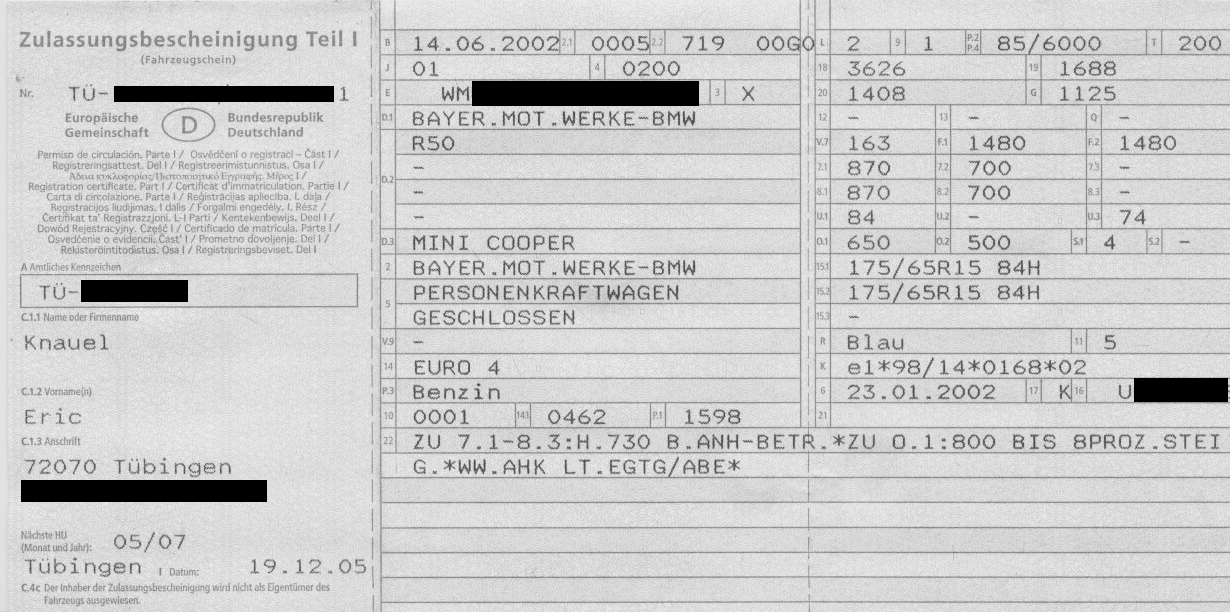
\includegraphics[width=\linewidth]{zusammengesetzte-daten/kfzschein-front}\\
      \medskip
      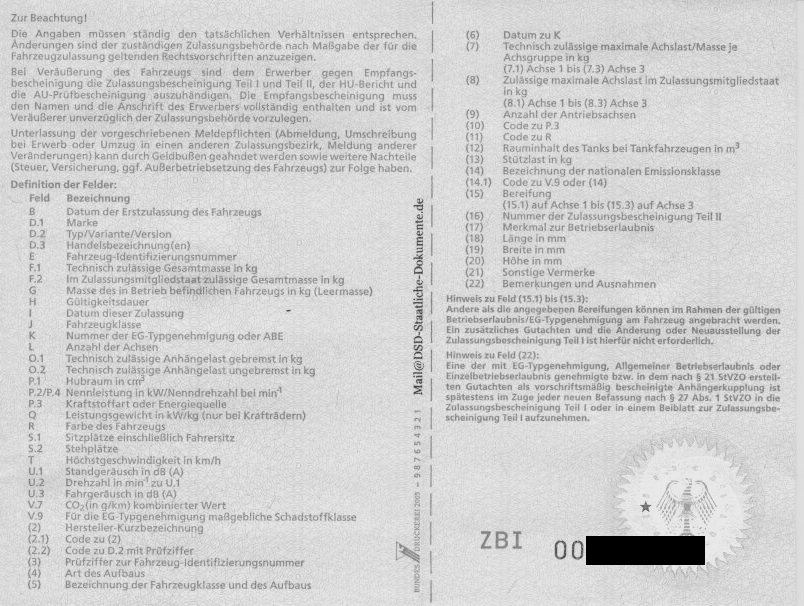
\includegraphics[width=\linewidth]{zusammengesetzte-daten/kfzschein-back}
      \caption{Vorder- und Rückseite eines Fahrzeugscheins}
      \label{fig:fahrzeugschein}
    \end{figure}
\end{aufgabe}

\begin{aufgabe}

  Schreibe für den Tübinger Stadtverkehr ein
  Programm, welches überprüft, ob ein Fahrzeug in den Umweltzonen fahren 
  darf.
  \begin{enumerate}
  \item Definiere einen Datentyp für Fahrzeuge. Dieser
    Datentyp soll den Typ, das Nummernschild und die Schadstoffklasse des
    Fahrzeuges beinhalten.
  \item Erstelle die Beispielfahrzeuge für die
    Fahrzeugtypen "<Stadtbus">, "<Reisebus">, "<Dieselauto">
    und "<Benzinauto">. Gehe davon aus, dass die Busse der
    Schadstoffklasse~2, das Dieselauto der Schadstoffklasse~3 und das
    Benzinauto der Schadstoffklasse~4 angehören.
  \item Schreibe eine Funktion \lstinline{fahrverbot?},
    welche überprüft, ob ein gegebenes Fahrzeug bei einer gegebenen
    Mindest-Schadstoffklasse noch fahren darf. Gestalte die Signatur
    so, dass er nur Mindest-Schadstoffklassen von 1 bis 4 akzeptiert.
  \item Die Mühlstraße in Tübingen ist in einer Richtung für
    alle Fahrzeuge außer Stadtbusse gesperrt. Schreibe eine Funktion
    \lstinline{sonderrecht?}, die überprüft, ob ein gegebenes Fahrzeug die
    Mühlstraße in der gesperrten Richtung befahren darf.  
  \item Der Stadtrat hat die Idee, den Tourismus
    dadurch anzukurbeln, dass Sonntags auch Reisebusse die Mühlstrasse in
    der gesperrten Richtunge befahren dürfen. Erweitere hierfür die
    Funktion \lstinline{sonderrecht?} um den Wochentag und lasse sonntags
    auch Reisebusse zu.
  \end{enumerate}
  Verwende beim Schreiben der Funktion die
  Konstruktionsanleitungen für Funktionen und für Fallunterscheidungen. 
  Schreibe Testfälle, die alle Möglichkeiten der   
  Fallunterscheidung abdecken.
  
\end{aufgabe}

\begin{aufgabe}

  Schreibe ein Programm für einen Paketdienst, das den Preis
  für ein Paket berechnet!
  \begin{enumerate}
    
  \item Schreibe eine Daten- und eine Record-Definition für
    \textit{Adressen}.  Zu einer Adresse gehören der Name, die Straße
    mit Hausnummer, die Postleitzahl, der Ort und das Land.
    
  \item Der Paketdienst verlangt einen Zuschlag für Sendungen, die
    international verschickt werden.  Schreibe eine Funktion
    \lstinline{international?}, die als Argument eine \textit{Adresse}
    bekommt und feststellt, ob die Adresse im Ausland liegt.

  \item Der Paketdienst hat einen Sondertarif für Sendungen, die
    innerhalb der gleichen Postleitzahl verschickt werden.  Schreibe
    eine Funktion \lstinline{same-zip-code?}, die als Argumente zwei
    \textit{Adressen} bekommt und feststellt, ob die Postleitzahlen
    und die Länder der beiden Adressen gleich sind.

  \item Ein Paket wird klassifiziert nach seinen Abmessungen.
    Schreibe eine Daten- und eine Record-Definition für
    \textit{Abmessungen}.  Abmessungen bestehen aus Länge, Breite und
    Höhe.

  \item Die Paketpreise richten sich nach der Größe des zu
    verschickenden Pakets.  Der Paketdienst verwendet die drei
    Größenklassen \textit{Small}, \textit{Medium} und \textit{Large},
    um die Kosten für das Paket zu berechnen.  Ausschlaggebendes
    Kriterium für die Paketgröße ist die Summe der längsten und der
    kürzesten Seite des Pakets.

    Schreibe eine Funktion
    \lstinline{add-longest-and-shortest-side}, die als Argument eine
    \textit{Abmessung} bekommt.  Der Rückgabewert von
    \lstinline{add-longest-and-shortest-side} soll die Summe der längsten
    und der kürzesten Seite der Abmessung sein.  Lagere die
    Teilprobleme in zwei Hilfsfunktionen aus: \lstinline{longest-side}
    und \lstinline{shortest-side}.

  \item Schreibe eine Daten- und eine Record-Definition für
    \textit{Pakete}.  Ein Paket hat eine Absender- und eine
    Empfängeradresse.  Benutze für die Adressen die bereits
    erstellte Record-Definition.  Außerdem hat ein Paket noch weitere
    Eigenschaften: Die Abmessungen (benutze dafür die bereits
    erstellte Record-Definition), das Gewicht, die Beförderungsdauer
    und eine Zusatz\-option Nachnahme.  Die Beförderungsdauer soll
    \emph{normal}, \emph{next-day} oder \emph{next-morning} sein.

  \item Schreibe eine Funktion \lstinline{parcel-size-class}, die
    als Argument ein \textit{Paket} bekommt und die Größenklasse
    zurückgibt.  Ausschlaggebend für die Paketgröße ist die Abmessung
    (siehe oben).  Folgende Tabelle enthält die Zuordnung von
    Paketgröße und Abmessung:

    \begin{center}
      \begin{tabular}{c|l}
        Paketgröße & Abmessung \\
        \hline
        S & 0--50 cm \\
        M & $>$50--100 cm \\
        L & $>$100 cm \\
      \end{tabular}
    \end{center}

  \item Schreibe eine Funktion \lstinline{calculate-base-postage},
    die als Argument ein \textit{Paket} bekommt und die
    Basis-Portokosten für dieses Paket berechnet.

    Lege dabei
    folgende Grundtariftabelle des Paketdienstes zugrunde:

    \begin{center}
      \begin{tabular}{c|ccc}
        & \multicolumn{3}{c}{Gewicht} \\
        Paketgröße & 0--5 kg & $>$5--10 kg & $>$10 kg \\
        \hline
        S & 3,00 & 6,00 & 9,00 \\
        M & 6,00 & 10,00 & 14,00 \\
        L & 9,00 & 15,00 & 21,00 \\
      \end{tabular}
    \end{center}

    

  \item Schreibe eine Funktion
    \lstinline{transportation-time-factor}, die als Argument ein
    \textit{Paket} bekommt und den Aufschlagsfaktor für die
    Beförderungsdauer zurückliefert.  Lege dabei folgende
    Aufschlagsfaktoren zugrunde:
    
    \begin{center}
      \begin{tabular}{c|ccc}
        & \multicolumn{3}{c}{Beförderungsdauer} \\
        Beförderungsdistanz & normal & next-day & next-morning \\
        \hline
        gleiche PLZ & -25\% & +0\% & +25\% \\
        Inland & +0\% & +50\% & +100\% \\
        Ausland & +100\% & +200\% & +300\% \\
      \end{tabular}
    \end{center}
    
  \item Schreibe eine Funktion
    \lstinline{cash-on-delivery-surcharge}, die als Argument ein
    \textit{Paket} bekommt und den Aufschlag für die Nachnahme
    zurückliefert.  Lege dabei folgende Aufschläge zugrunde:

    \begin{center}
      \begin{tabular}{c|c}
        Beförderungsdistanz & Nachnahmegebühr \\
        \hline
        Inland & +3,00 \\
        Ausland & +9,00 \\
      \end{tabular}
    \end{center}

  \item Schreibe eine Funktion \lstinline{calculate-postage}, die
    als Argument ein \textit{Paket} bekommt und die Portokosten
    berechnet.  Benutze dafür die bereits programmierten
    Lösungen der verschiedenen Teilprobleme.
    
  \end{enumerate}
  
\end{aufgabe}

%%% Local Variables: 
%%% mode: latex
%%% TeX-master: "i1"
%%% End: 


% Diese Datei ist Teil des Buchs "Schreibe Dein Programm!"
% Das Buch ist lizensiert unter der Creative-Commons-Lizenz
% "Namensnennung - Weitergabe unter gleichen Bedingungen 4.0 International (CC BY-SA 4.0)"
% https://creativecommons.org/licenses/by-sa/4.0/deed.de

\chapter{Gemischte Daten}
\label{cha:gemischte-daten}

Manchmal kommen an einer Stelle in unserem Problem verschiedene
Klassen der gleichen Sorte Daten vor:
%
\begin{itemize}
\item Ein Tier kann ein Gürteltier oder ein Papagei sein.
\item Eine Koordinate kann eine kartesische Koordinate oder eine
  Polarkoordinate sein.
\item Ein Essen kann ein Frühstück, Mittagessen oder Abendessen sein.
\end{itemize}
%
Solche Daten heißen \textit{gemischte Daten\index{gemischte
    Daten}}, und es handelt sich um eine weitere Form von
Falluntscheidungen, neben den aus Kapitel~\ref{cha:conditionals}
bekannten Aufzählungen und Zahlenbereichen.

Obwohl die Daten verschiedenartig sind, unterstützen sie doch
gemeinsame Operationen: Das Gewicht eines Tiers kann sowohl für
Gürteltiere als auch Papageien berechnet werden, der Abstand vom
Ursprung kann für beide Koordinatendarstellungen berechnet werden, die
Anzahl der Gänge kann für jede Art Essen bestimmt werden.

\section{Gemischte Daten}
\label{sec:mixed-data}
\label{sec:animal}

\mentioncode{gemischte-daten/animal.rkt}
%
In der Einleitung war die Rede von Papageien:\index{Papagei} die benutzen wir, um
gemischte Daten einzuführen.  Vorher müssen wir jedoch Papageien mit den bekannten
Mitteln definieren.  Wir erweitern dafür die Datei mit dem Gürteltier
aus dem vorigen Kapitel.

Genau wie bei Gürteltieren interessiert uns bei Papageien das Gewicht,
aber wir nehmen an, da Papageien in der Regel nicht auf texanischen
Highways überfahren werden, dass sie immer lebendig sind.  Außerdem
betrachten wir ausschließlich sprechende Papageien, die jeweils einen
einzelnen Satz sagen können.  Hier die Datendefinition:
%
\begin{lstlisting}
; Ein Papagei hat folgende Eigenschaften:
; - Gewicht in Gramm
; - Satz, den er sagt
\end{lstlisting}
%
Hier die dazu passende Record-Definition:
%
\begin{lstlisting}
(define-record parrot
  make-parrot
  (parrot-weight   natural)
  (parrot-sentence string))
\end{lstlisting}
%
\ldots{} und die passenden Signaturen:
%
\begin{lstlisting}
(: make-parrot (natural string -> parrot))
(: parrot-weight (parrot -> natural))
(: parrot-sentence (parrot -> string))
\end{lstlisting}
%
Hier zwei Beispiele für Papageien mit Kommentaren, die die Beziehung
zwischen Daten und Information beschreiben:
%
\begin{lstlisting}
(define parrot1 (make-parrot 10000 "Der Gärtner war's.")) ; 10kg, Miss Marple
(define parrot2 (make-parrot 5000 "Ich liebe Dich.")) ; 5kg, Romantiker 
\end{lstlisting}
%
Du kannst Dir vielleicht vorstellen, dass Papageien und
Gürteltiere sich in einem Programm begegnen, also \emph{gemischt}
vorkommen.  Papageien und Gürteltiere gehören zum gemeinsamen
Oberbegriff \textit{Tier}\index{Tier}.  Dafür könnte eine
Beschreibung so aussehen:

\medskip

\noindent Ein \textit{Tier} ist eins der folgenden:
% 
\begin{itemize}
\item ein Gürteltier
\item ein Papagei
\end{itemize}
%
Die Formulierung "<eins der folgenden"> ist Dir schon aus
Abschnitt~\ref{sec:datendefinition} und
Konstruktionsanleitung~\ref{ka:fallunterscheidung} auf
Seite~\pageref{ka:fallunterscheidung} bekannt: Sie deutet auf eine
Fallunterscheidung\index{Fallunterscheidung} hin.

Da aber Gürteltiere und Papageien nicht als nur jeweils ein Wert
repräsentiert sind, handelt es sich nicht um eine Aufzählung: Die
beiden Fälle der Fallunterscheidung beschreiben unterschiedliche
\textit{Klassen}\index{Klasse} von Tieren, jede mit ihrer eigenen
Signatur.  Damit liegt eine neue Organisation von Daten vor:
\textit{gemischte Daten}.\index{gemischte Daten} Entsprechend ist es
durchaus sinnvoll, nach dem "<Gewicht eines Tiers"> zu fragen oder
"<ein Tier zu füttern">, was wir im folgenden auch vorhaben.

Die Beschreibung des Begriffs "<Tier"> ist bereits als Datendefinition
geeignet, und muss für Inklusion im Programm nur als Kommentar
umformatiert werden:
%
\begin{lstlisting}
; Ein Tier ist eins der folgenden:
; - Gürteltier
; - Papagei
\end{lstlisting}
%
Bei zusammengesetzen Daten kann die Datendefinition in eine
Record-Definition überführt werden.  In diesem Fall ist für jede
einzelne Klasse
Tier jeweils schon eine Record-Definition da.  Wenn wir Tiere im
allgemeinen in
Funktionen verarbeiten wollen, brauchen wir allerdings eine Signatur
für Tiere.  Zum Beispiel wollen wir eine Funktion schreiben, die für jedes
Tier das Gewicht ermittelt.  Diese Funktion könnte folgende Signatur haben:
%
\begin{lstlisting}
(: animal-weight (animal -> natural))
\end{lstlisting}
%%% HK: das \textbf war wohl ein Irrtum?
Wir brauchen also eine Definition für die Signatur \lstinline{animal}.
Diese sieht folgendermaßen aus:
%
\begin{lstlisting}
(define animal
  (signature
    (mixed dillo parrot)))
\end{lstlisting}
%
Das \lstinline{signature} kennen wir von den Fallunterscheidungen aus
Abschnitt~\ref{page:signature} auf Seite~\pageref{page:signature}.
Das \lstinline{mixed}\index{mixed@\texttt{mixed}} ist neu und steht
für "<gemischte Daten">, also Fallunterscheidungen, bei denen jeder
Fall seine eigene Signatur hat.  Du kannst die obige Definition lesen als
"<Tiere sind gemischt aus Gürteltieren und Papageien">; das klingt
aber auf Deutsch hölzern, weshalb wir für die Datendefinition bei der
Formulierung "<eins der folgenden"> bleiben.  Mit der Definition steht
die Signatur \lstinline{animal} zur Verfügung.  Wir haben schon mit der
Signatur für \lstinline{animal-weight} vorgegriffen.  Hier ist sie noch
einmal zusammen mit einer Kurzbeschreibung:
%
\begin{lstlisting}
; Gewicht eines Tiers feststellen
(: animal-weight (animal -> natural))
\end{lstlisting}
%
Diese Funktion sollte entsprechend für Gürteltiere \emph{und}
Papageien funktionieren, wir brauchen also Testfälle für beide:
%
\begin{lstlisting}
(check-expect (animal-weight dillo1) 55000)
(check-expect (animal-weight dillo2) 58000)
(check-expect (animal-weight parrot1) 10000)
(check-expect (animal-weight parrot2) 5000)
\end{lstlisting}
%
Das Gerüst sieht so aus:
%
\begin{lstlisting}
(define animal-weight
  (lambda (animal)
    ...))
\end{lstlisting}
%
Tiere bilden auch eine Fallunterscheidung in den Daten, mit zwei
Fällen: Gürteltiere und Papageien.  Im Rumpf der Funktion brauchen wir
also eine Verzweigung mit zwei Zweigen:
%
\begin{lstlisting}
(define animal-weight
  (lambda (animal)
    (cond
      (... ...)
      (... ...))))
\end{lstlisting}
%
Wir brauchen als Nächstes zwei Bedingungen~-- eine, die Gürteltiere
und eine, die Papageien identifiziert.  Dafür erweitern wir die
Record-Definitionen um ein neues Element, das \textit{Prädikat}\index{Prädikat}.
Die Prädikate werden uns erlauben, die Bedingungen zu
schreiben.  Die Record-Definitionen sehen dann so aus:
%
\begin{lstlisting}
(define-record dillo
  make-dillo
  dillo? ; |\(\Longleftarrow\)| Prädikat
  (dillo-weight natural)
  (dillo-alive? boolean))

(define-record parrot
  make-parrot
  parrot? ; |\(\Longleftarrow\)| Prädikat
  (parrot-weight   natural)
  (parrot-sentence string))
\end{lstlisting}
%
Es sind zwei neue Namen hinzugekommen, \lstinline{dillo?} und
\lstinline{parrot?}. Das sind die Prädikate, und sie haben folgenden
Signaturen:
%
\begin{lstlisting}
(: dillo? (any -> boolean))
(: parrot? (any -> boolean))
\end{lstlisting}
%
Das \lstinline{any} ist auch neu und ist die Signatur für einen
beliebigen Wert: Ein Prädikat kann also auf absolut alles angewendet
werden.  Die beiden Prädikate unterscheiden Gürteltiere
beziehungsweise Papageien von anderen Werten:
%
\begin{lstlisting}
(dillo? dillo1)
|\evalsto| #t
(dillo? parrot1)
|\evalsto| #f
(parrot? dillo1)
|\evalsto| #f
(parrot? parrot1)
|\evalsto| #t
(dillo? 5)
|\evalsto| #f
(parrot? "foo")
|\evalsto| #f
\end{lstlisting}
%
Im allgemeinen ist ein Prädikat eine Funktion mit der Signatur
\lstinline{(any -> boolean)}, die für eine bestimmte Sorte von Werten
\lstinline{#t} liefert, für alle andere Werte aber \lstinline{#f}.  In
diesem speziellen Fall identifizieren die Prädikate \lstinline{dillo?}
und \lstinline{parrot?} jeweils alle Werte, die zu einem bestimmten
Record-Typ gehören.  Prädikate müssen aber nicht zu einem Record-Typ
gehören, wir können ein Prödikat auch selber schreiben.  Außerdem sind
eine Reihe von Prädikaten vordefiniert~-- dazu mehr später in diesem
Kapitel auf \pageref{scheme:predicates}.

\begin{aufgabeinline}
  Schreibe ein Prädikat namens \lstinline{animal?} für alle Tiere,
  also alle Werte, die ein \lstinline{dillo}-Record oder ein
  \lstinline{parrot}-Record sind.
\end{aufgabeinline}
%
Die Prädikate \lstinline{dillo?}  und \lstinline{parrot?}  können wir
benutzen, um die Bedingungen aus der Schablone zu bestücken:
%
\begin{lstlisting}
(define animal-weight
  (lambda (animal)
    (cond
      ((dillo? animal) ...)
      ((parrot? animal) ...))))
\end{lstlisting}
%
Im ersten Zweig~-- dem Zweig für Gürteltiere~-- kommt nun
\lstinline{dillo-weight} zum Einsatz, im zweiten Zweig~-- für
Papageien~-- ist \lstinline{parrot-weight} zuständig:
%
\begin{lstlisting}
(define animal-weight
  (lambda (animal)
    (cond
      ((dillo? animal) (dillo-weight animal))
      ((parrot? animal) (parrot-weight animal)))))
\end{lstlisting}
% 
Fertig!

\begin{feature}{\texttt{define-record} (mit Prädikaten)}{scheme:define-record-predicates}
Eine \lstinline{define-record}-Form\index{define-record@\texttt{define-record}}
hat folgende allgemeine Gestalt:
%
\begin{lstlisting}
(define-record |\(t\)|
  |\(c\)|
  |\(p\)|
  (|\(\mathit{sel}\sb{1}\)| |\(\mathit{sig}\sb{1}\)|)
  |\(\ldots\)|
  (|\(\mathit{sel}\sb{n}\)| |\(\mathit{sig}\sb{n}\)|))
\end{lstlisting}
%
Diese Form definiert einen Record-Typ mit $n$ Feldern.
Dabei sind $t$, $c$, $\mathit{sel}_1 \ldots \mathit{sel}_n$ allesamt Variablen, für die
\lstinline{define-record} Definitionen anlegt:
%
\begin{itemize}
\item $t$ ist der Name der Record-Signatur.
\item $c$ ist der Name des Konstruktors mit 
  folgender Signatur:
%  
\begin{lstlisting}
(: |\(c\)| (|\(\mathit{sig}\sb{1}\)| |\(\ldots\)| |\(\mathit{sig}\sb{n}\)| -> |\(t\)|))
\end{lstlisting}
\item $p$ ist der Name des Prädikats, der Records diesen Typs von
  anderen Werten unterscheidet.  Das Prädikat kann auch weggelassen
  werden.

    Das Prädikat hat folgende Signatur:
\begin{lstlisting}
(: |\(p\)| (any -> boolean))
\end{lstlisting}
\item $\mathit{Sel}_1, \ldots, \mathit{sel}_n$ sind die Namen der Selektoren für die Felder
  des Record-Typs.  Der Selektor $\mathit{sel}_i$ hat folgende Signatur:
% 
\begin{lstlisting}
(: |\(\mathit{sel}\sb{i}\)| (|\(t\)| -> |\(\mathit{sig}\sb{i}\)|))
\end{lstlisting}
\end{itemize}
%
\end{feature}
%
Abbildung~\ref{scheme:define-record-predicates} ist eine
aktualisierte Beschreibung der Form von
\lstinline{define-record}, bei der auch Prädikate
berücksichtigt sind

Aus diesem Beispiel ergibt sich eine Konstruktionsanleitung für
gemischte Daten.  Zunächst die Datenanalyse:

\begin{konstruktionsanleitung}{Gemischte Daten: Datenanalyse}
  \label{ka:gemischt-datenanalyse}
  Gemischte Daten sind Fallunterscheidungen, bei denen jeder Fall eine
  eigene Klasse von Daten mit eigener Signatur ist.
  Schreibe bei gemischten Daten eine Signatur-Definition der folgenden Form unter die
  Datendefinition:
%
\begin{lstlisting}
(define |\(\mathit{sig}\)|
  (signature
    (mixed |\(\mathit{sig}\sb{1}\)| |\(\mathit{sig}\sb{2}\)| |\(\ldots\)| |\(\mathit{sig}\sb{n}\)|)))
\end{lstlisting}
$\mathit{Sig}$ ist die Signatur für die neue Datensorte; $\mathit{sig}_1$ bis $\textit{sig}_n$
sind die Signaturen, aus denen die neue
Datensorte zusammengemischt ist.
\end{konstruktionsanleitung}
%
\noindent Die Konstruktionsanleitung für die Schablone ist der aus
der Konstruktionsanleitung~\ref{ka:fallunterscheidung-schablone} für
Fallunterscheidungen auf
Seite~\pageref{ka:fallunterscheidung-schablone} ähnlich:
%
\begin{konstruktionsanleitung}{Gemischte Daten als Eingabe:
    Schablone}
  \label{ka:gemischt-eingabe-schablone}
Eine Schablone für eine Funktion und deren Testfälle, die gemischte
Daten akzeptiert, kannst Du folgendermaßen konstruieren:
%
\begin{itemize}
\item Schreibe Tests für jeden der Fälle.
\item  Schreibe eine \lstinline{cond}-Verzweigung als Rumpf in die
  Schablone, die genau $n$ Zweige hat~-- also genau soviele Zweige,
  wie es Fälle in der Datendefinition beziehungsweise der Signatur gibt.
\item Schreibe für jeden Zweig eine Bedingung, der den entsprechenden
  Fall identifiziert.
\item Vervollständige die Zweige, indem Du eine Datenanalyse für
  jeden einzelnen Fall vornimmst und entsprechende Hilfsfunktionen
  und Konstruktionsanleitungen benutzt.
  Die übersichtlichsten Programme entstehen meist, wenn für jeden Fall
  separate Hilfsfunktionen definiert sind.\label{page:separate-mixed-procs}
\end{itemize}
%
\end{konstruktionsanleitung}
%
Eine Konstruktionsanleitung oder Schablone für gemischte Daten
\emph{als Ausgabe} ist unnötig~-- Du benutzt einfach die Schablone
des entsprechenden Falls.

Beachte den Unterschied zwischen \lstinline{enum} und
\lstinline{mixed}, die leicht zu verwechseln sind: \lstinline{enum} steht
für "<einer der folgenden \emph{Werte}">, während \lstinline{mixed} für
"<gehörend zu einer der folgenden \emph{Signaturen}"> steht.

\begin{aufgabeinline}
  Denk Dir sinnvolle Datendefinitionen für Frühstück, Mittagessen und
  Abendessen aus (ein \ldots{}essen besteht aus \ldots), so dass es
  Sinn ergibt, für jede Sorte Essen die Frage "<Was für ein Gemüse ist
  enthalten?"> zu stellen.  Schreibe zunächst für jede Sorte Essen
  eine Funktion, die das enthaltene Gemüse liefert.  Schreibe dann
  eine Datendefinition für den Oberbegriff "<Essen">; ein Essen kann
  ein Frühstück, ein Mittagessen oder ein Abendessen sein.  Schreibe
  eine Funktion, welche das enthaltene Gemüse für ein Essen liefert.
\end{aufgabeinline}

\section{Gemischte Daten als Ausgabe}
\label{sec:feed-animal}

Wir können einen Papagei ähnlich wie ein Gürteltier füttern~-- nur die
Portion ist kleiner, wir nehmen 50~g an.  Kurzbeschreibung und Signatur:\index{feed-parrot@\texttt{feed-parrot}}
%
\begin{lstlisting}
; Papagei mit 50 g Futter füttern
(: feed-parrot (parrot -> parrot))
\end{lstlisting}
%
Testfälle:
%
\begin{lstlisting}
(check-expect (feed-parrot parrot1) (make-parrot 10050 "Der Gärtner war's."))
(check-expect (feed-parrot parrot2) (make-parrot 5050 "Ich liebe Dich."))
\end{lstlisting}
%
Gerüst:
%
\begin{lstlisting}
(define feed-parrot
  (lambda (parrot)
    ...))
\end{lstlisting}
%
Die Schablone entsteht aus der Kombination der Schablonen für
zusammengesetzte Daten
als Einage (Konstruktionsanleitung~\ref{ka:zusammengesetzt-eingabe-schablone} auf
Seite \pageref{ka:zusammengesetzt-eingabe-schablone}) und als Ausgabe
(Konstruktionsanleitung~\ref{ka:zusammengesetzt-ausgabe-schablone} auf
Seite \pageref{ka:zusammengesetzt-ausgabe-schablone}):
%
\begin{lstlisting}
(define feed-parrot
  (lambda (parrot)
    (make-parrot ... ...)
    ... (parrot-weight parrot) ...
    ... (parrot-sentence parrot) ...))
\end{lstlisting}
%
\ldots{} und schließlich der vollständige Rumpf:
%
\begin{lstlisting}
(define feed-parrot
  (lambda (parrot)
    (make-parrot (+ (parrot-weight parrot) 50)
                 (parrot-sentence parrot))))
\end{lstlisting}
%
Nun können wir eine Funktion schreiben, die ein beliebiges Tier
akzeptiert und es füttert.  Hier Kurzbeschreibung und Signatur:
%
\begin{aufgabe}
; Tier füttern
(: feed-animal (animal -> animal))
\end{aufgabe}
%
Die Funktion soll sich genauso verhalten wie \lstinline{feed-dillo}
beziehungsweise \lstinline{feed-parrot}.  Das können wir direkt als
Tests ausdrücken:
%
\begin{lstlisting}
(check-expect (feed-animal parrot1) (feed-parrot parrot1))
(check-expect (feed-animal parrot2) (feed-parrot parrot2))
(check-expect (feed-animal dillo1) (feed-dillo dillo1))
(check-expect (feed-animal dillo2) (feed-dillo dillo2))
\end{lstlisting}
%
Das Gerüst sieht so aus:
%
\begin{lstlisting}
(define feed-animal
  (lambda (animal)
    ...))
\end{lstlisting}
%
Da die Eingabe gemischt ist, brauchen wir eine Verzweigung mit soviel
Zweigen wie \lstinline{animal} Fälle hat, also zwei, die wir gleich
mit den passenden Bedingungen versehen:
%
\begin{lstlisting}
(define feed-animal
  (lambda (animal)
    (cond
      ((dillo? animal) ...)
      ((parrot? animal) ...))))
\end{lstlisting}
%
Schließlich müssen wir noch die Antworten ergänzen, für die wir die
Funktionen benutzen, die wir schon geschrieben haben:
%
\begin{lstlisting}
(define feed-animal
  (lambda (animal)
    (cond
      ((dillo? animal) (feed-dillo animal))
      ((parrot? animal) (feed-parrot animal)))))
\end{lstlisting}
%
Das Beispiel zeigt, dass wir keine spezielle Konstruktionsanleitung
für gemischte Daten als Ausgabe brauchen: Wir müssen nur darauf
achten, den jeweils richtigen Fall zu liefern.
%
\begin{aufgabeinline}
  Schreibe eine Funktion \lstinline{run-over-animal}, die ein Tier
  überfährt!
\end{aufgabeinline}

\section{Die Lebensmittelampel}

\mentioncode{gemischte-daten/zuckerampel.rkt}
%
In diesem Abschnitt nehmen wir uns noch ein weiteres Beispiel für
gemischte Daten vor, diesmal von vorneherein unter Benutzung der
Konstruktionsanleitung aus dem vorigen Abschnitt.

Die Lebensmittelampel ist eine Kennzeichnung auf Lebensmittelverpackungen,
die den Gehalt von gesundsheitsrelevanten Nährstoffen in den
Ampelfarben ausweist: Grün für niedrigen Gehalt, Gelb für mittleren Gehalt und
Rot für hohen Gehalt. Bei Zucker zum Beispiel sieht die Ampel so aus, bezogen
auf 100~g eines Lebensmittels:
%
\begin{center}
  \begin{tabular}{l|l|l}
    grün & niedriger Gehalt &  weniger als 5 g\\
    gelb & mittlerer Gehalt & zwischen 5 g und 22,5 g\\
    rot & hoher Gehalt & mehr als 22,5 g
  \end{tabular}
\end{center}
%
Trotz der Bemühungen der Europäischen Union sind die
Bezeichnungen uneinheitlich.  Technisch gesehen ist die Ampel
redundant, wenn der Zuckergehalt in Gramm angegeben ist.
Manchmal ist allerdings der Zuckergehalt auch separat für Fruktose und
Glukose angegeben.

Ein Computerprogramm könnte aber den Umgang erleichtern, indem es jede
Angabe auf einer Lebensmittelpackung~-- Zucker in Gramm insgesamt,
Fruktose und Glukose separat sowie die Ampel~-- in die einheitliche
Ampel-Form bringt.  Schreiben wir also ein solches Programm.  Zunächst
die Datenanalyse:
%
\begin{itemize}
\item Die Zuckermenge in Gramm ist eine (rationale) Zahl.
\item Zuckeranteile bestehen aus der Menge von Fruktose und Glukose.
\item Eine Zuckerampel ist rot, gelb oder grün.
\item Der Zuckergehalt kann entweder als Zuckermenge, Zuckeranteile
  oder Zuckerampel angegeben werden.
\end{itemize}
%
Hier ist die Datendefinition für die zusammengesetzen Zuckeranteile:
%
\begin{lstlisting}
; Zuckeranteile bestehen aus:
; - Fruktose-Menge (in g)
; - Glukose-Menge (in g)
\end{lstlisting}
%
Daraus ergibt sich direkt die Record-Definition mit zwei Komponenten,
jeweils rationale Zahlen:
%
\begin{lstlisting}
(define-record sugars
  make-sugars
  sugars?
  (sugars-fructose-g rational)
  (sugars-glucose-g  rational))
\end{lstlisting}
%
Hier einige Beispiele, zusammen mit Kommentaren, die die Beziehung
zwischen Daten und Information beschreiben:
%
\begin{lstlisting}
(define s1 (make-sugars 1 1)) ; 1 g Fruktose, 1 g Glukose
(define s2 (make-sugars 2 3)) ; 2 g Fruktose, 3 g Glukose
(define s3 (make-sugars 5 5)) ; 5 g Fruktose, 5 g Glukose
(define s4 (make-sugars 10 2.5)) ; 10 g Fruktose, 2.5 g Glukose
(define s5 (make-sugars 10 13)) ; 10 g Fruktose, 13 g Glukose
(define s6 (make-sugars 15 10)) ; 15 g Fruktose, 10 g Glukose
\end{lstlisting}
%
Bei der Ampel selbst handelt es sich um eine einfache
Fallunterscheidung:
%
\begin{lstlisting}
; Eine Ampel ist einer der folgenden Werte:
; - rot
; - gelb
; - grün
\end{lstlisting}
%
Das ist eine Aufzählung, wir geben entsprechend der dazu passenden
Signatur einen Namen:
%
\begin{lstlisting}
(define traffic-light
  (signature
   (enum "red" "yellow" "green")))
\end{lstlisting}
%
Die Angabe über den Zuckergehalt kann jede der drei oben genannten Formen
annehmen:
%
\begin{lstlisting}
; Ein Zuckergehalt ist eins der folgenden:
; - Gewicht in Gramm
; - Zuckeranteile
; - Ampelbezeichnung
\end{lstlisting}
%
Wieder ist an der Formulierung erkennbar, dass es sich um gemischte
Daten handelt, und zwar mit drei Fällen.  Das übersetzen wir in ein
Signatur-Definition mit \lstinline{mixed} und ebenfalls drei Fällen:
%
\begin{lstlisting}
(define sugar-content
  (signature
   (mixed rational
          sugars
          traffic-light)))
\end{lstlisting}
%
Das Beispiel zeigt, dass die Fälle einer Definition für gemischte Daten
nicht allesamt Records sein müssen.  Es ist allerdings wichtig, dass
die Fälle \emph{disjunkt} sind, also jeder Wert eindeutig einem der
Fälle zugeordnet werden kann: Sonst wäre es nicht möglich, eine sinnvolle
Verzweigung zu schreiben, welche die Fälle unterscheidet.

Nun zu unserer Funktion zur Ermittlung der Ampelbezeichnung für den
Zuckergehalt.  Hier Kurzbeschreibung und Signatur:
%
\begin{lstlisting}
; Ampelbezeichnung für Zuckergehalt ermitteln
(: sugar-traffic-light (sugar-content -> traffic-light))
\end{lstlisting}
%
Wir brauchen ziemlich viele Testfälle, um alle Fälle von
Zuckergehalt abzudecken sowie die Eckfälle der Tabelle von oben.
%
\begin{lstlisting}
(check-expect (sugar-traffic-light 2) "green")
(check-expect (sugar-traffic-light 5) "yellow")
(check-expect (sugar-traffic-light 10) "yellow")
(check-expect (sugar-traffic-light 12.5) "yellow")
(check-expect (sugar-traffic-light 23) "red")

(check-expect (sugar-traffic-light s1) "green")
(check-expect (sugar-traffic-light s2) "yellow")
(check-expect (sugar-traffic-light s3) "yellow")
(check-expect (sugar-traffic-light s4) "yellow")
(check-expect (sugar-traffic-light s5) "red")
(check-expect (sugar-traffic-light s6) "red")

(check-expect (sugar-traffic-light "green") "green")
(check-expect (sugar-traffic-light "yellow") "yellow")
(check-expect (sugar-traffic-light "red") "red")
\end{lstlisting}
%
Als Nächstes ist, wie immer, das Gerüst dran:
%
\begin{lstlisting}
(define sugar-traffic-light
  (lambda (sugar-content)
    ...))
\end{lstlisting}         
%
Als Nächstes wenden wir die Schablone für Funktionen an, die gemischte
Daten akzeptieren.  Wir brauchen eine Verzweigung mit sovielen Zweigen
wie \lstinline{sugar-content} Fälle hat, also drei:
%
\begin{lstlisting}
(define sugar-traffic-light
  (lambda (sugar-content)
    (cond
      (... ...)
      (... ...)
      (... ...))))
\end{lstlisting}         
%
Als Nächstes brauchen wir Tests für die drei Fälle.  Für den zweiten
Fall ist das einfach, da es sich um \lstinline{sugars}-Records handelt:
da gibt es das Prädikat \lstinline{sugars?}.  Beim ersten Fall handelt es
sich aber um eine rationale Zahl, beim dritten um eine Zeichenkette~--
beides eingebaute Datensorten.  Für diese gibt es die eingebauten
Prädikate \lstinline{rational?} und \lstinline{string?}~--
Abbildung~\ref{scheme:predicates} zählt noch mehr eingebaute
Prädikate auf.
%
\begin{feature}{Eingebaute Prädikate}{scheme:predicates}
  \index{Prädikate!eingebaut}\index{eingebaute Prädikate}
  Folgende Prädikate sind eingebaut:
  \begin{itemize}
  \item \lstinline{number?}\index{number?@\texttt{number?}} testet, ob ein Wert eine Zahl ist.
  \item \lstinline{real?}\index{real?@\texttt{real?}} testet, ob ein Wert eine reelle Zahl ist.
  \item \lstinline{rational?}\index{rational?@\texttt{rational?}} testet, ob ein Wert eine rationale Zahl ist.
  \item \lstinline{natural?}\index{natural?@\texttt{natural?}} testet, ob ein Wert eine natürliche Zahl ist.
  \item \lstinline{string?}\index{string?@\texttt{string?}} testet, ob ein Wert eine Zeichenkette ist.
  \item \lstinline{boolean?}\index{boolean?@\texttt{boolean?}} testet, ob ein Wert ein boolescher Wert ist.
  \end{itemize}
\end{feature}
%
Mit dieser Information gewappnet können wir die Tests ergänzen:
%
\begin{lstlisting}
(define sugar-traffic-light
  (lambda (sugar-content)
    (cond
      ((rational? sugar-content) ...)
      ((sugars? sugar-content) ...)
      ((string? sugar-content) ...))))
\end{lstlisting}         
%
Im ersten Zweig handelt es sich nicht nur um eine rationale Zahl,
sondern auch um eine Fallunterscheidung mit drei Fällen entsprechend
der Tabelle vom Anfang:
%
\begin{lstlisting}
(define sugar-traffic-light
  (lambda (sugar-content)
    (cond
      ((rational? sugar-content) 
       (cond
         (... ...)
         (... ...)
         (... ...)))
      ((sugars? sugar-content) ...)
      ((string? sugar-content) ...))))
\end{lstlisting}         
%
Als Nächstes ergänzen wir Tests entsprechend der Tabelle:
%
\begin{lstlisting}
(define sugar-traffic-light
  (lambda (sugar-content)
    (cond
      ((rational? sugar-content) 
       (cond
         ((< sugar-content 5) ...)
         ((and (>= sugar-content 5) (<= sugar-content 12.5)) ...)
         ((> sugar-content 12.5) ...)))
      ((sugars? sugar-content) ...)
      ((string? sugar-content) ...))))
\end{lstlisting}         
%
Schließlich müssen wir noch die Antworten eintragen:
%
\begin{lstlisting}
(define sugar-traffic-light
  (lambda (sugar-content)
    (cond
      ((rational? sugar-content) 
       (cond
         ((< sugar-content 5) "green")
         ((and (>= sugar-content 5) (<= sugar-content 12.5)) "yellow")
         ((> sugar-content 12.5) "red")))
      ((sugars? sugar-content) ...)
      ((string? sugar-content) ...))))
\end{lstlisting}         
%
Das verschachtelte \lstinline{cond} ist etwas unübersichtlich: In
Konstruktionsanleitung~\ref{ka:gemischt-eingabe-schablone} auf
Seite~\pageref{page:separate-mixed-procs} ist bereits vermerkt, dass
es sinnvoll ist, diesen Zweig in eine separate Hilfsfunktion
auszulagern.  Hier sind Kurzbeschreibung und Signatur für diese
Hilfsfunktion:
%
\begin{lstlisting}
; Zuckeranteil in g in Ampel umwandeln
(: sugar-weight->traffic-light (rational -> traffic-light))
\end{lstlisting}
%
Die Testfälle lassen sich aus den Testfällen für
\lstinline{sugar-traffic-light} durch einfaches Kopieren und Umbenennen
gewinnen:
%
\begin{lstlisting}
(check-expect (sugar-weight->traffic-light 2) "green")
(check-expect (sugar-weight->traffic-light 5) "yellow")
(check-expect (sugar-weight->traffic-light 10) "yellow")
(check-expect (sugar-weight->traffic-light 12.5) "yellow")
(check-expect (sugar-weight->traffic-light 23) "red")
\end{lstlisting}
%
Gerüst:
%
\begin{lstlisting}
(define sugar-weight->traffic-light
  (lambda (sugar-weight)
    ...))
\end{lstlisting}
%
Den Rumpf haben wir ja schon geschrieben, wir müssen ihn nur noch
hierher bewegen und \lstinline{sugar-content} in \lstinline{sugar-weight} umbenennen. Das \drscheme{}-System
bietet dazu nach einem Klick auf "<Syntaxprüfung"> die Möglichkeit, mit einem
Rechtsklick auf den Parameter \lstinline{sugar-content} ein Menü aufzuklappen, das unter
anderem die Auswahl "<\lstinline{sugar-content} umbenennen"> anbietet. \drscheme{} sorgt dann
dafür, dass alle zugehörigen Vorkommen von \lstinline{sugar-content} in gleicher Weise
umbenannt werden.\label{def:sugar-weight-traffic-light}
%
\begin{lstlisting}
(define sugar-weight->traffic-light
  (lambda (sugar-weight)
    (cond
      ((< sugar-weight 5) "green")
      ((and (>= sugar-weight 5) (<= sugar-weight 22.5)) "yellow")
      ((> sugar-weight 12.5) "red"))))
\end{lstlisting}
%
Zurück zu \lstinline{sugar-traffic-light}: Dort benutzen wir zunächst die
neu definierte Hilfsfunktion:
%
\begin{lstlisting}
(define sugar-traffic-light
  (lambda (sugar-content)
    (cond
      ((rational? sugar-content)
       (sugar-weight->traffic-light sugar-content))
      ((sugars? sugar-content) ...)
      ((string? sugar-content) ...))))
\end{lstlisting}         
%
Beim nächsten Zweig geht es um den Fall \lstinline{sugars}~--
zusammengesetzte Daten.  Wir können also die entsprechende Schablone
anwenden:
%
\begin{lstlisting}
(define sugar-traffic-light
  (lambda (sugar-content)
    (cond
      ((rational? sugar-content)
       (sugar-weight->traffic-light sugar-content))
      ((sugars? sugar-content) ... (sugars-fructose-g sugar-content) ...
                   ... (sugars-glucose-g sugar-content) ...)
      ((string? sugar-content) ...))))
\end{lstlisting}         
%
Wir müssen Fruktose- und den Glukose-Anteil addieren und die Summe
dann ebenfalls entsprechend der Tabelle vom Anfang in eine Ampelfarbe
umwandeln.  Aber halt!~-- Genau für das Umwandeln der Zahl aus der
Tabelle in eine Ampelfarbe haben wir ja gerade die Hilfsfunktion
\lstinline{sugar-weight->traffic-light} geschrieben, und diese
können wir
erneut zum Einsatz bringen:
%
\begin{lstlisting}
(define sugar-traffic-light
  (lambda (sugar-content)
    (cond
      ((rational? sugar-content)
       (sugar-weight->traffic-light sugar-content))
      ((sugars? sugar-content)
       (sugar-weight->traffic-light
         (+ (sugars-fructose-g sugar-content)
            (sugars-glucose-g sugar-content))))
      ((string? sugar-content) ...))))
\end{lstlisting}         
%
Bleibt der letzte Fall~-- der ist zum Glück trivial, da es sich schon
um eine Farbe handelt, Die muss \lstinline{sugar-traffic-light} nur
zurückgeben:
%
\begin{lstlisting}
(define sugar-traffic-light
  (lambda (sugar-content)
    (cond
      ((rational? sugar-content)
       (sugar-weight->traffic-light sugar-content))
      ((sugars? sugar-content)
       (sugar-weight->traffic-light 
         (+ (sugars-fructose-g sugar-content)
            (sugars-glucose-g sugar-content))))
      ((string? sugar-content) sugar-content))))
\end{lstlisting}         
%
Fertig!

\section{Fehler repräsentieren}
\label{sec:slope}
\label{sec:maybe}

\mentioncode{gemischte-daten/slope.rkt}
%
Dieser Abschnitt beschreibt eine weitere häufig vorkommende Anwendung
für gemischte Daten.  Es geht um Situationen, wo eine Funktion
keine sinnvolle Antwort weiß.

Als Beispiel schreiben wir eine Funktion, welche die Steigung einer
Geraden auf der Ebene berechnet anhand der Koordinaten zweier Punkte
darauf.  Die Funktion akzeptiert vier Argumente: Die X- und die Y-Koordinate des
ersten Punkts und danach die X- und die Y-Koordinate des zweiten
Punkts.  Wir fangen mit Kurzbeschreibung, Signatur, einigen Tests
und einem Gerüst an:
%
\begin{lstlisting}
; Steigung einer Gerade berechnen
(: slope (real real real real -> real))

(check-expect (slope 0 0 1 1) 1)
(check-expect (slope 0 0 2 1) 1/2)
(check-expect (slope 1 2 3 5) 3/2)

(define slope
  (lambda (x1 y1 x2 y2)
    ...))
\end{lstlisting}
%
Die Formelsammlung sagt, dass wir zur Berechnung der Steigung die
Differenz der Y-Koordinaten durch die Differenz der X-Koordinaten
teilen müssen:
%
\begin{lstlisting}
(define slope
  (lambda (x1 y1 x2 y2)
    (/ (- y2 y1)
       (- x2 x1))))
\end{lstlisting}
%
Fertig, könnte man meinen.  Es gibt aber Linien, die keine Steigung
haben.  In der REPL sieht das so aus:
%
\begin{alltt}
> (slope 0 0 0 1)
{\color{red}/: durch 0 geteilt}
\end{alltt}
%
Die Meldung ist ein bisschen unfreundlich und birgt mehrere Probleme:
%
\begin{itemize}
\item Die Meldung besagt zwar, was das Programm gemacht hat (durch 0
  geteilt), aber benennt nicht die Ursache des Problems: dass die
  Gerade keine Steigung hat.
\item Das Programm bricht einfach ab, ohne dass es eine Möglichkeit
  bekommt, mit dem Problem umzugehen.
\item Dass das Programm einfach abbrechen kann, ist aus der Signatur
  nicht ersichtlich, die suggeriert, dass die Funktion immer eine
  reelle Zahl zurückliefert.
\end{itemize}
%
Alle drei Probleme können wir auf einmal mit gemischten Daten lösen.
Dazu müssen wir zunächst dafür sorgen, dass die Funktion einen
sinnvollen Wert zurückliefert, bevor sie durch 0 teilen würde.
Dadurch werden die Eingaben in zwei Klassen aufgeteilt: Es gibt eine
Steigung oder eben nicht.  Es bietet sich eine binäre Verzweigung an,
um diese beiden Klassen zu unterscheiden:
%
\begin{lstlisting}
(define slope
  (lambda (x1 y1 x2 y2)
    (if (= (- x2 x1) 0)
        ...
        (/ (- y2 y1)
           (- x2 x1))))) 
\end{lstlisting}
%
Nur müssen wir anstelle der Ellipse irgendetwas ins Programm
schreiben.  Wir können nicht einfach irgendeine reelle Zahl nehmen, da
diese ja auch eine legitime Steigung sein könnte.  Stattdessen
brauchen wir einen Wert, den wir von den legitimen Zahlen
unterscheiden können.  Wir könnten eine spezielle Zeichenkette oder
\lstinline{#f} benutzen.  (Siehe dazu Aufgabe~\ref{aufgabe:no-slope}
auf Seite~\pageref{aufgabe:no-slope}.)

Wir empfehlen aber, stattdessen einen eigenen Record-Typ zu
definieren, und zwar so:
%
\begin{lstlisting}
; Es gibt keine Steigung
(define-record no-slope
  make-no-slope
  no-slope?)
\end{lstlisting}
%
Dieser Record-Typ hat keine Felder, das heißt, er kann nur benutzt
werden, um einen einzigen Wert herzustellen, nämlich
\lstinline{(make-no-slope)}.  (Es handelt sich also um eine
degenerierte Version von zusammengesetzten Daten ohne Bestandteile.)
Diesen Wert können wir aber durch das Prädikat \lstinline{no-slope?}
von allen anderen Werten unterscheiden und benutzen ihn, wenn es keine
Steigung gibt:
%
\begin{lstlisting}
(define slope
  (lambda (x1 y1 x2 y2)
    (if (= (- x2 x1) 0)
        (make-no-slope)
        (/ (- y2 y1)
           (- x2 x1)))))
\end{lstlisting}
%
Jetzt können wir einen Testfall definieren:
%
\begin{lstlisting}
(check-expect (no-slope? (slope 0 0 0 1)) #t)
\end{lstlisting}
%
Allerdings liefert \drscheme{} für diesen Testfall eine
Signaturverletzung: Die Signatur tut ja immer noch so, als würde immer
eine reelle Zahl herauskommen.  Wir erweitern sie also folgendermaßen:
%
\begin{lstlisting}
(: slope (real real real real -> (mixed real no-slope)))
\end{lstlisting}
%
Dieser Signatur sieht man unmittelbar an, was sie liefert und kann aus
den Namen auch schließen, was die beiden Fälle bedeuten.  Natürlich
könnten wir eine eigene Signatur definieren wie sonst bei gemischten
Daten, das lohnt aber hier kaum.

\section*{Aufgaben}

\begin{aufgabe}
  Vereinfache in der Funktion \lstinline{sugar-weight->traffic-light} auf
  Seite~\pageref{def:sugar-weight-traffic-light} die Bedingungen, wie
  in Abschnitt~\ref{page:bedingungen-vereinfachen} auf
  Seite~\pageref{page:bedingungen-vereinfachen} beschrieben.
\end{aufgabe}

\begin{aufgabe}
  Ein Supermarkt möchte seine Waren in einem Programm verwalten. Es gibt
  drei Warenklassen:
  \begin{description}
  \item[Essen] beschrieben durch einen Namen, den Stückpreis, das Mindesthaltbarkeitsdatum
    und den aktuellen Bestand im Supermarkt
  \item[Getränke] beschrieben durch einen Namen, den Stückpreis, das Mindesthaltbarkeitsdatum
    und den Bestand. Zusätzlich muss hier noch festgehalten werden, ob Pfand verlangt wird.
  \item[Sonstige] beschrieben durch einen Namen, den Stückpreis und den Bestand.
  \end{description}

  
  \begin{enumerate}
  \item Führe eine Datenanalyse durch und erstelle Daten- und 
    Record-Definitionen.
  \item Schreibe eine Funktion \lstinline{stückpreis}, die eine Warenklasse
    akzeptiert und den Stückpreis zurückgibt.
  \item Schreibe eine Funktion \lstinline{buchen}, die eine Warenklasse und die Anzahl der
    abzubuchenden Exemplare akzeptiert, den Bestand der Warenklasse reduziert und die
    Warenklasse zurückgibt. Falls mehr Exemplare gefordert werden, als in der Warenklasse
    vorhanden sind, soll der Bestand auf 0 gesetzt werden.
  \item Schreibe eine Funktion \lstinline{haltbar?}, die eine
    Warenklasse und ein Datum akzeptiert und \lstinline{#t} zurückgibt, falls das
    Mindesthaltbarkeitsdatum (MHD) nicht überschritten wurde. Falls kein MHD bekannt ist,
    soll \lstinline{#t} zurückgeben werden.
  \end{enumerate}
\end{aufgabe}

\begin{aufgabe}
  \label{aufgabe:knaubichler}
  Auf seinen Reisen um die Welt trifft Dr.~Sperber
  viele interessante und skurrile Zeitgenossen. Unter ihnen
  Dr.~Knaubichler, ein Experte auf dem Gebiet der Kreuzung von
  mystischen Kreaturen.  Es gibt drei klassische Grundkreaturen:

  \begin{itemize}
  \item Der Garnolaf, der Stärke besitzt.
  \item Das Ronugor, das Wissen besitzt.
  \item Der Tschipotol, der Risikobereitschaft besitzt.
  \end{itemize}
  %
  Die Merkmale der Kreaturen sind unterschiedlich ausgeprägt.  Die
  Knaubichler"=Kreaturenmerkmal"=Skala geht von 0 bis 100.  Die
  Grundkreaturen haben jeweils nur ein Merkmal, keine besitzt ein
  Merkmal einer anderen Grundkreatur.

  Nun kreuzt Dr.~Knaubichler die Grundkreaturen miteinander. Es
  entstehen also
  \begin{itemize}
  \item Das Ronulaf, mit Wissen und Stärke.
  \item Der Tschigor, mit Wissen und Risikobereitschaft.
  \item Das Lapotol, mit Stärke und Risikobereitschaft.
  \item Der Tschirgaronu, Wissen, Stärke und Risikobereitschaft.
  \end{itemize}
  %
  Leider erben die Kreuzungen nicht die vollen Merkmale beider
  Grundkreaturen.

  Bei der Kreuzung unterschiedlicher Grunkreaturen gilt folgendes:
  Bei der Kreuzung von Ronugor und Tschipotol wird
  das übernommene Wissen um 10\% veringert; bei Tschipotol und
  Garnolaf hingegen nimmt die Risikobereitschaft um 5\% ab, aber die
  Stärke legt um 8\% zu. Garnolaf und Ronugor lassen die Stärke um 5\%
  zulegen. Kreuzt man alle drei Grundkreaturen, nimmt jede Eigenschaft
  um 3\% ab.
  
  Werden zwei Kreaturen der gleichen Sorte gekreuzt, so entsteht eine
  neue Kreatur mit $\frac{2}{3}$ der addierten Eigenschaften der
  beiden Grundkreaturen. Man kann nur Grundkreaturen kreuzen.

  In jedem Fall kann eine Eigenschaft maximal den Wert 100
  haben.
    
  Dr.~Knaubichler braucht ein Programm, welches die neue Kreatur
  berechnet, bevor er die Kreuzungen durchführt.  Hilf ihm
  dabei!
  
  \begin{enumerate}

  \item Mache eine Datenanalyse und erstelle
    passende Daten- und Record-Definitionen.  Gib alle
    Signaturen der Record-Funktionen an!

  \item Schreibe für jede der oben aufgelisteten
    Kreuzungen von zwei Grundkreaturen eine Funktion, die die Kreuzung
    vornimmt und eine neue Kreatur zurückgibt.
  \end{enumerate}
\end{aufgabe}


\begin{aufgabe}
  \label{aufgabe:knaubichler2}
  Erweitere die Lösung von Aufgabe~\ref{aufgabe:knaubichler}:
  
  \begin{enumerate}
  \item Schreibe eine Funktion, die zwei
    Grundkreaturen in beliebiger Reihenfolge akzeptiert, die Kreuzung
    vornimmt und eine neue Kreatur zurückgibt.
    
  \item Schreibe eine
    Funktion, die drei Grundkreaturen in beliebiger Reihenfolge
    akzeptiert, die Kreuzung vornimmt und eine neue Kreatur
    zurückgibt.
  \end{enumerate}
\end{aufgabe}     

\begin{aufgabe}

  Das Spiele-Entwicklungsteam von
  \textit{Exciting Games, Inc.} ist in Personalnot: Für die
  Programmierung des bahnbrechenden 2D-Spiels \textit{The Adventures
    of DrRacket} wird dringend eine Repräsentation der grafischen
  Formen Kreis, Rechteck und Dreieck benötigt.  Alle Hacker
  sind leider wahnsinnig damit beschäftigt, bunte Pixel in der Gegend
  herumzuschieben und können sich daher nicht dieser grundlegenden
  Aufgabe widmen.  Deswegen fällt Dir diese Aufgabe zu!  Dir geht
  nur ein mit Pizzabelag verschmierter Zettel zu, der offenbar als
  Arbeitsanweisung gedacht ist.  Darauf steht:
  \begin{itemize}

  \item Es gibt drei Klassen von Formen: Kreise, Rechtecke und
    gleichschenklige Dreiecke.  Alle Formen haben eine
    Ursprungskoordinate und enthalten eine Information über die Größe
    (Radius, Höhe, Breite, etc), wie Du auf der Abbildung siehst.
    Benutze für die Ursprungskoordinate die vorgegebenen kartesischen
    Koordinaten!

    % \begin{figure}[h]
    \begin{center}
      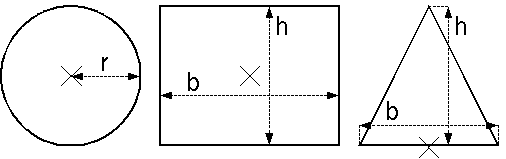
\includegraphics[height=1.8cm]{gemischte-daten/shapes.png}
      % \caption{Formen}
      % \label{Formen}
    \end{center}
    % \end{figure}

  \item Es soll Funktionen geben, die auf allen Formen funktionieren
    und Folgendes leisten:

    \begin{itemize}

    \item kartesische Koordinate einer Form zurückgeben

    \item $x$-Koordinate einer Form zurückgeben

    \item $y$-Koordinate einer Form zurückgeben

    \item Abstand des Ursprungs einer Form zum Ursprung des
      Koordinatensystems zurückgeben

    \item Flächeninhalt einer Form zurückgeben

    \item Form um $\Delta_x$ in $x$-Richtung und um $\Delta_y$ in
      $y$-Richtung verschieben, also eine Form zurückgeben, deren
      Ursprungskoordinate entsprechend verschoben ist

%     \item Größe einer Form um einen Faktor ändern, also eine Form
%       zurückgeben, deren Größe entsprechend angepasst ist
  \item  Flächeninhalt zweier
    Formen vergleichen: Für gleich große Formen liefert die Funktion
    \verb|"equal"| zurück, sonst \verb|"smaller"|, wenn die erste
    Form kleiner ist, beziehungsweise \verb|"bigger"|, wenn die erste
    Form größer ist.
    \end{itemize}

  \end{itemize}
  %
  Zeige den Hackern, was richtiges Software-Engineering ist und
  benutze die passenden Konstruktionsanleitungen, um Repräsentationen für die Formen und die zugehörigen
  Funktionen zu schreiben!
\end{aufgabe}

\begin{aufgabe}

  Es gibt verschiedene Verstöße gegen die
  Straßenverkehrsordnung: 
  \begin{itemize}
  \item Falschparken mit Ort und Zeitpunkt des Verstoßes

  \item Überfahren einer roten Ampel mit Ort und Zeitpunkt des Verstoßes
    sowie der Dauer in Sekunden, wie lange die Ampel bereits rot war

  \item Überhöhte Geschwindigkeit mit Ort und Zeitpunkt des Verstoßes
    sowie der Höhe der Geschwindigkeits"-über"-tre"-tung
  \end{itemize}
  Neben den angegebenen Bestandteilen muss später für jeden Verstoß vermerkt 
  werden, ob zusätzlich eine "<Gefährdung des Straßenverkehrs"> vorliegt.
  
  \begin{enumerate}
  \item Schreibe eine Datendefinition für
    Verstöße gegen die Straßenverkehrsordnung.  Schreibe Daten-
    und Record-Definitionen für die verschiedenen Verstöße.  
    Die Zeitpunkte kannst Du durch Zeichenketten wie \verb|"11.4.1971 22:00"| repräsentieren.  
    Gib alle Signaturen an!

  \item Schreibe eine Funktion, die einen
    beliebigen Verstoß entgegennimmt und den Ort des Verstoßes
    zurückgibt.

    Schreibe analog eine Funktion, die einen
    beliebigen Verstoß entgegennimmt und den Zeitpunkt des Verstoßes
    zurückgibt.

  \item Schreibe eine Funktion, die einen
    beliebigen Verstoß entgegennimmt, diesen als Gefährdung des
    Straßenverkehrs betrachtet und wieder zurückgibt (das heißt jeder 
    Verstoß ist ein Verstoß mit Gefährdung).
  \end{enumerate}

  Die Verstöße haben unterschiedliche Tatbestände zur Folge:

  \begin{itemize}
  \item Einfaches Vergehen mit Bußgeld

  \item Ordnungswidrigkeit mit Bußgeld, Punkte für die
    Verkehrssünderdatei und Fahrverbot in Monaten

  \item Straftat mit Punkten für die Verkehrssünderdatei und
    Freiheitsstrafe in Monaten
  \end{itemize}
  
  \begin{enumerate} \setcounter{enumii}{3}
  \item Schreibe eine Datendefinition für
    Tatbestände auf Verstöße gegen die Straßenverkehrsordnung.
    Schreibe Daten- und Record-Definitionen für die verschiedenen
    Tatbestände.  Gib alle Signaturen an!

  \item Schreibe eine Funktion, die einen
    beliebigen Tatbestand akzeptiert und die Anzahl der anfallenden
    Punkte zurückliefert.
  \end{enumerate}

  Schreibe nun Funktionen, die Verstöße akzeptieren und die
  Tatbestände berechnen:

  \begin{enumerate} \setcounter{enumii}{5}
  \item Schreibe eine Funktion, die Falschparken
    akzeptiert und ein einfaches Vergehen mit 20~Euro Bußgeld zurückgibt.
    Wenn das Falschparken eine Gefährdung des Straßenverkehrs
    darstellt (zum Beispiel bei Behinderung von Rettungsfahrzeugen),
    soll die Funktion eine Ordnungswidrigkeit mit 40~Euro Bußgeld,
    einem Punkt und keinem Fahrverbot zurückgeben.

  \item Schreibe eine Funktion, die Überfahren
    einer roten Ampel akzeptiert und eine Ordnungswidrigkeit
    zurückgibt.  Dabei gilt:
    \begin{itemize}
    \item wenn die Ampel kürzer als eine Sekunde rot war und keine
      Gefährdung vorlag: 50~Euro, 3~Punkte, kein Fahrverbot
    \item wenn die Ampel mindestens eine Sekunde rot war oder eine
      Gefährdung vorlag: 125~Euro, 4~Punkte, 1~Monat Fahrverbot
    \end{itemize}

  \item Schreibe eine Funktion, die überhöhte
    Geschwindigkeit akzeptiert und den Tatbestand zurückgibt.  Dabei
    gilt:
    \begin{itemize}
    \item Geschwindigkeitsübertretung weniger als 20 km/h ohne Gefährdung:
      einfaches Vergehen mit 35~Euro
    \item Geschwindigkeitsübertretung zwischen 20 und 40 km/h
      (inklusive) ohne Gefährdung: Ordnungswidrigkeit mit 75~Euro,
      3~Punkten und 1~Monat Fahrverbot
    \item Geschwindigkeitsübertretung von mehr als 40 km/h ohne
      Gefährdung: Ordnungswidrigkeit mit 200~Euro, 4~Punkte und
      3~Monate Fahrverbot
    \item bei gleichzeitiger Gefährdung des Straßenverkehrs: Straftat
      mit 3~Punkte mehr als ohne Gefährdung angegeben und
      Freiheitsstrafe, die doppelt so lang ist wie das Fahrverbot, das
      ohne Gefährdung gilt (wenn es kein Fahrverbot gibt, dann gibt es
      auch keine Freiheitsstrafe)
    \end{itemize}

  \item Schreibe eine Funktion, die einen
    Verstoß akzeptiert und dessen Folge zurückgibt.  Benutze die
    Funktionen aus den vorherigen Teilaufgaben.
  \end{enumerate}
\end{aufgabe}

\begin{aufgabe}\label{aufgabe:no-slope}
  Experimentiere für die Funktion \lstinline{slope} in
  Abschnitt~\ref{sec:slope} auf Seite~\pageref{sec:slope}
  mit anderen Repräsentationen als einem eigenen
  Record-Typ für "<keine Steigung">:
  %
  \begin{itemize}
  \item Liefere \lstinline{#f} zurück.
  \item Liefere eine Zeichenkette \lstinline{"no slope"} zurück.
  \end{itemize}
  %
  Wie muss jeweils die Signatur von \lstinline{slope} lauten?
  
  Wie könnte ein Programm dann nach einem Aufruf feststellen, ob es
  keine Steigung gab?  Schreibe für beide Varianten einen Ersatz für das Prädikat
  \lstinline{no-slope?}, das diese Situation feststellt.

  Was haben die insgesamt drei Varianten für die Repräsentation von
  "<keine Steigung"> jeweils für Vor- und Nachteile?
\end{aufgabe}

%%% Local Variables: 
%%% mode: latex
%%% TeX-master: "i1"
%%% End: 


% Diese Datei ist Teil des Buchs "Schreibe Dein Programm!"
% Das Buch ist lizensiert unter der Creative-Commons-Lizenz
% "Namensnennung - Weitergabe unter gleichen Bedingungen 4.0 International (CC BY-SA 4.0)"
% https://creativecommons.org/licenses/by-sa/4.0/deed.de

\chapter{Programmieren mit Selbstbezügen und Kombinatoren}
\label{cha:selbstbezug}

Bisher haben wir nur Daten vorgestellt, die
eine feste Größe haben und damit im Wortsinn beschränkt sind.  Viele
Informationen haben aber eine variable Größe: Die Bücher im Regal werden
immer mehr, Bauwerke bestehen aus variabel vielen Bauteilen.  Um
solche Informationen als Daten zu repräsentieren, stellen wir in
diesem Kapitel einen weiteren Aspekt der Datenanalyse vor, den
\textit{Selbstbezug}\index{Selbstbezug}.  Hier sind einfache
Beispiele:
%
\begin{itemize}
\item Ein Fluss besteht aus Hauptfluss und Nebenfluss~-- beides wieder
  Flüsse.
\item Ein Dateiverzeichnis auf dem Computer kann 
  Unterverzeichnisse enthalten.
\item Ein großer Bücherstapel besteht aus einem etwas kleineren
  Bücherstapel und einem weiteren Buch.
\end{itemize}
%
Bei all diesen Beispielen werden aus kleineren Dingen größere gemacht:
Aus zwei Flüssen, die zusammenfließen, wird ein großer Fluss.  Aus
mehreren Dateien und Verzeichnissen wird ein großes Verzeichnis.  Aus
einem kleinen Bücherstapel wird ein großer.  In der Programmierung
nennen wir das Bauen von großen Dingen aus kleinen Dingern derselben
Sorte \textit{kombinieren}. Die Funktionen, die das erledigen, heißen
\textit{Kombinatoren}\index{Kombinator}: Um die geht es in diesem Kapitel.

\section{Flüsse abbilden}

\mentioncode{selbstbezuege/river.rkt}

\begin{figure}[tbh]
  \centering
\begin{tikzpicture}
  [
    confluence/.style = {shape=rectangle, rounded corners,
                         draw, align=center},
    absent/.style = {},
    grow                    = left,
    sibling distance        = 6em,
    level distance          = 10em,
    % makes arrows the opposite direction from -latex
    edge from parent/.style = {draw,latex-},
    every node/.style       = {font=\footnotesize}
    ]
    \node [absent] {}
    child {
      node [confluence] {Epfendorf}
        child {
          node [confluence] {Tieringen}
          edge from parent node [below] {Schlichem} }
        child { node  [confluence] {Rottweil}
          child { node [confluence] {Heimliswald}
            edge from parent node [below] {Eschach} }
          child { node [confluence] {Dreifaltigkeitsberg}
            edge from parent node [below] {Prim} } } };
\end{tikzpicture}
  \caption{Der Neckar nahe der Quellen}
  \label{fig:neckar}
\end{figure}

\noindent Abbildung~\ref{fig:neckar} ist ein Diagramm, das die
Struktur des Neckar nahe der Quellen beschreibt: Er fließt zunächst
aus den Bächen Eschach und Prim zusammen, und danach fließen immer
weitere Bäche und Flüsse hinzu~-- in der Abbildung noch die
Schlichem.

Die Struktur eines Flusses werden wir durch Daten abbilden, um danach
eine Funktion zu schreiben, die feststellt, ob ein Fluss durch einen
bestimmten Ort fließt.  Unser erster Versuch einer Datendefinition
sieht so aus:
%
\begin{lstlisting}
; Ein Fluss kommt entweder aus:
; - einer Quelle
; - einem Hauptfluss und einem Nebenfluss
\end{lstlisting}
%
Man kann zwar schon sehen, dass es sich um eine Fallunterscheidung
handelt, aber wir können die Formulierung schärfen, um klar zu machen,
dass es sich um gemischte Daten handelt:
%
\begin{lstlisting}
; Ein Fluss ist eins der folgenden:
; - ein Bach aus einer Quelle
; - ein Zusammentreffen von einem Hauptfluss und einem Nebenfluss
\end{lstlisting}
%
Daraus können wir direkt eine Signatur-Definition machen:
%
\indexvariable{river}
\begin{lstlisting}
(define river
  (signature (mixed creek confluence)))
\end{lstlisting}
%
Die Datendefinitionen für "<Bach"> und "<Zusammentreffen"> fehlen
allerdings noch.  In Abbildung~\ref{fig:neckar} steht an den Bächen
jeweils noch der Name.  Eine passende Datendefinition sieht so aus:
%
\begin{lstlisting}
; Ein Bach hat folgende Eigenschaften:
; - Ursprungsort
\end{lstlisting}
%
Das klingt ein bisschen komisch, weil der Bach ja nur \emph{eine}
Eigenschaft hat, aber die Datendefinition trotzdem zusammengesetzte
Daten beschreibt.  Trotzdem ist das legitim und korrekt~-- niemand
wird sagen wollen, dass der Ursprungsort der Bach \emph{ist}.
Außerdem kannst Du Dir vorstellen, dass ein Bach später noch mehr
Eigenschaften bekommt, die wir in den Daten festhalten
wollen. (Wasserqualität oder Fließgeschwindigkeit zum Beispiel.)
Entsprechend ist es auch sinnvoll, dafür eine Record-Definition zu
schreiben:
%
\indexvariable{creek}
\begin{lstlisting}
(define-record creek
  make-creek
  creek?
  (creek-origin string))
\end{lstlisting}
%
Wenn später noch weitere Eigenschaften hinzukommen, können wir die
Record-Definition erweitern, ohne anderen Code zu beeinträchtigen.

Kommen wir zu den Zusammentreffen.  Auch hier ist ein Ort relevant~--
dort, wo sie zusammentreffen.  Außerdem ist wichtig, \emph{welche}
Flüsse oder Bäche da zusammentreffen.  Die Datendefinition könnte so
aussehen:
%
\begin{lstlisting}
; Ein Zusammentreffen besteht aus:
; - Ort
; - Hauptfluss
; - Nebenfluss
\end{lstlisting}
%
Die Formulierung zeigt eindeutig, dass es sich um zusammengesetzte
Daten handelt.  Aber diese Datendefinition weist eine Auffälligkeit
auf, die erst sichtbar wird, wenn wir sie im Zusammenhang der
Gesamt-Datendefinition für Flüsse betrachten:
%
\tikzstyle{every picture}+=[remember picture]
\tikzstyle{fluss} = [shape=rectangle,inner sep=0pt,text depth=0pt]
%
\begin{lstlisting}
; Ein |\tikz\node[fluss](fluss){\textbf{Fluss}};| ist eins der folgenden:
; - |\ldots|
; - ein Zusammentreffen |\ldots|
|\ldots|
; Ein Zusammentreffen besteht aus:
; - Ort
; - Haupt|\tikz\node[fluss](fluss1){\textbf{fluss}};|
; - Neben|\tikz\node[fluss](fluss2){\textbf{fluss}};|
\end{lstlisting}
%
\begin{tikzpicture}[overlay]
  \path[->,blue,thick](fluss1) edge [out=0, in=0] (fluss);
  \path[->,blue,thick](fluss2) edge [out=0, in=0] (fluss);
\end{tikzpicture}
%
Die Datendefinition für "<Fluss"> benutzt selbst den Begriff
"<Fluss">.   Noch offensichtlicher wird das, wenn wir die dazu
passende Record-Definition erstellen:
%
\indexvariable{confluence}
\begin{lstlisting}
(define-record confluence
  make-confluence
  confluence?
  (confluence-location  string)
  (confluence-main-stem river)
  (confluence-tributary river))
\end{lstlisting}
%
In der Definition von \texttt{confluence} wird \texttt{river} benutzt
und umgekehrt.  Das ist nichts schlimmes~-- im Gegenteil, diese beiden
\textit{Selbstbezüge}\index{Selbstbezug} erlauben uns, ganz
unterschiedliche Flüsse zu beschreiben, insbesondere solche
unterschiedlicher Größe.  Den Abschnitt des Neckar in~\ref{fig:neckar}
können wir so abbilden:
%
\indexvariable{eschach}
\indexvariable{prim}
\indexvariable{neckar-1}
\indexvariable{neckar-1}
\indexvariable{schlichem}
\begin{lstlisting}
(define eschach (make-creek "Heimliswald")) ; Quelle des Neckar
(define prim (make-creek "Dreifaltigkeitsberg")) ; Quelle des Neckar
; erster Zusammenfluss des Neckar:
(define neckar-1 (make-confluence "Rottweil" eschach prim))
; Zufluss des Neckar:
(define schlichem (make-creek "Tieringen")) 
; zweiter Zusammenfluss des Neckar:
(define neckar-2 (make-confluence "Epfendorf" neckar-1 schlichem))
\end{lstlisting}
%
An diesen Beispielen sieht man sehr schön, dass
\texttt{make-confluence} zwei Flüsse zu einem kombiniert~-- es handelt
sich um einen \textit{Kombinator}\index{Kombinator}.

Wir hatten angekündigt, eine Funktion zu schreiben, die feststellt, ob
Wasser von einem bestimmten Ort in einen Fluss fließt.  Wir machen das
wieder nach Vorschrift, also zuerst die Kurzbeschreibung:
%
\begin{lstlisting}
; Fließt Wasser von einem Ort in Fluss?
\end{lstlisting}
%
In der Kurzbeschreibung sind schon die Substantive "<Fluss"> und
"<Ort"> als Eingaben aufgeführt, die übertragen wir in die Signatur.
Da die Funktion eine Ja-/Nein-Frage beantwortet, liefert sie einen
booleschen Wert und hat ein Fragezeichen hinten am Namen:
%
\begin{lstlisting}
(: flows-from? (string river -> boolean))
\end{lstlisting}
%
Bei den Tests achten wir darauf, dass wir sowohl Bäche als auch Flüsse
testen, und sowohl Fälle, bei denen \lstinline{#t} als auch solche,
bei denen \lstinline{#f} herauskommt:
%
\begin{lstlisting}
(check-expect (flows-from? "Heimliswald" eschach) #t)
(check-expect (flows-from? "Tübingen" eschach) #f)
(check-expect (flows-from? "Heimliswald" neckar-2) #t)
(check-expect (flows-from? "Rottweil" neckar-2) #t)
(check-expect (flows-from? "Berlin" neckar-2) #f)
\end{lstlisting}
%
Das Gerüst ergibt sich wie immer direkt aus der Signatur:
%
\begin{lstlisting}
(define flows-from?
  (lambda (location river)
    ...))
\end{lstlisting}
%
Da es sich bei \lstinline{river} um gemischte Daten handelt, können
wir die Schablone dafür ergänzen.  Da \lstinline{river} zwei Fälle hat
(Bäche und Zusammenflüsse), muss die Schablone zwei Zweige haben.  Die
Bedingungen sind Aufrufe der jeweiligen Prädikate für
\lstinline{creek} und \lstinline{confluence}:
%
\begin{lstlisting}
(define flows-from?
  (lambda (location river)
    (cond
      ((creek? river) ...)
      ((confluence? river) ...))))
\end{lstlisting}
%
Nun können wir Code für die beiden Zweige ergänzen.  Fangen wir mit
den Bächen an.  Da es sich bei \lstinline{creek} um zusammengesetzte
Daten handelt (mit nur einem Bestandteil), sollte der Aufruf des
Selektors im Rumpf vorkommen:
%
\begin{lstlisting}
(define flows-from?
  (lambda (location river)
    (cond
      ((creek? river)
       ...
       (creek-origin river)
       ...)
      ((confluence? river)
       ...))))
\end{lstlisting}
%
Der Selektor \lstinline{creek-origin} liefert den Ursprungsort.  Wenn dieser dem
gesuchten Ort entspricht, so fließt der Fluss durch diesen Ort, sonst
nicht.  Im ersten Fall sollte \lstinline{#t} herauskommen, im zweiten
\lstinline{#f}.  Das sieht so aus:
%
\begin{lstlisting}
(define flows-from?
  (lambda (location river)
    (cond
      ((creek? river)
       (if (string=? (creek-origin river) location)
           #t
           #f))
      ((confluence? river)
       ...))))
\end{lstlisting}
%
Dieser Code kann noch etwas vereinfacht werden: Der
\lstinline{if}-Ausdruck sagt ja salopp formuliert:
%
\begin{quote}
  Wenn \lstinline{(string=? (creek-origin river) location)} als
  Resultat \lstinline{#t} liefert, dann \lstinline{#t}, und wenn es
  \lstinline{#f} liefert, dann \lstinline{#f}.
\end{quote}
%
Da reicht es auch, \lstinline{(string=? (creek-origin river) location)} hinzuschreiben.
%
\begin{aufgabeinline}\label{aufgabe:iftruefalse}
  Kannst Du diese Vereinfachung auf \lstinline{if}-Ausdrücken
  verallgemeinern und als Gleichung schreiben?
\end{aufgabeinline}
%
Als Nächstes können wir uns um den anderen Fall kümmern,
\lstinline{confluence}.  Auch dort handelt es sich um
zusammengesetzte Daten, wir können also schon einmal die
Selektoraufrufe hinschreiben:
%
\begin{lstlisting}
(define flows-from?
  (lambda (location river)
    (cond
      ((creek? river)
       (string=? (creek-origin river) location))
      ((confluence? river)
       ...
       (confluence-location river)
       (confluence-main-stem river)
       (confluence-tributary river)
       ...))))
\end{lstlisting}
%
Soweit die Schablone, wir können uns also Gedanken zur eigentlichen
Aufgabe machen.

Als erstes steht da \lstinline{(confluence-main-stem river)} der Ort
des Zusammenflusses.  Wenn es sich dabei um den gesuchten Ort handelt,
können wir die Frage, ob der Wasser von diesem Ort in den Fluss fließt, bereits
mit "<ja"> beziehungsweise \lstinline{#t} beantworten:
%
\begin{lstlisting}
(define flows-from?
  (lambda (location river)
    (cond
      ((creek? river)
       (string=? (creek-origin river) location))
      ((confluence? river)
       (if (string=? (confluence-location river) location)
           #t
           ...
           (confluence-main-stem river)
           (confluence-tributary river)
           ...)))))
\end{lstlisting}
%
Aber was, wenn der Ort des Zusammenflusses nicht der gesuchte Ort ist?
Dann müssen wir uns an die beiden anderen
Selektor-Aufrufe halten, die uns den Haupt- und den Nebenfluss des
Zusammenflusses liefern.  Wenn der eine oder der andere Wasser aus dem
gesuchten Ort enthält, dann könnten wir die Frage unserer Funktion
ebenfalls mit "<ja"> beantworten.  Dazu müssten wir also feststellen:
%
\begin{enumerate}
\item Fließt Wasser vom Ort \lstinline{origin} in den Hauptfluss?
\item Fließt Wasser vom Ort \lstinline{origin} in den Nebenfluss?
\end{enumerate}
%
Nun, wir schreiben ja gerade eine Funktion, die feststellt, ob Wasser
von einem bestimmten Ort in einen bestimmten Fluss fließt.  Können wir
die benutzen?  Wir schreiben das mal hin:
%
\begin{lstlisting}
(define flows-from?
  (lambda (location river)
    (cond
      ((creek? river)
       (string=? (creek-origin river) location))
      ((confluence? river)
       (if (string=? (confluence-location river) location)
           #t
           ...
           (flows-from? location (confluence-main-stem river))
           (flows-from? location (confluence-tributary river))
           ...)))))
\end{lstlisting}
%
Die beiden Aufrufe von \lstinline{flows-from?} entsprechen gerade
den beiden Fragen von oben.  Wir können ihre Ergebnisse kombinieren,
um unsere Antwort zu errechnen: Wenn Wasser aus \lstinline{location}
durch den Hauptfluss fließt \emph{oder} der Wasser aus
\lstinline{location} in den Nebenfluss fließt, so fließt auch Wasser
von \lstinline{location} in den "<Gesamtfluss">.  So sieht das aus:
%
\indexvariable{flows-from?}
\begin{lstlisting}
(define flows-from?
  (lambda (location river)
    (cond
      ((creek? river)
       (string=? (creek-origin river) location))
      ((confluence? river)
       (if (string=? (confluence-location river) location)
           #t
           (or
            (flows-from? location (confluence-main-stem river))
            (flows-from? location (confluence-tributary river))))))))
\end{lstlisting}
%
Fertig!

In dieser Funktion passiert etwas Besonderes, das es in den
Funktionen davor noch nicht gab: Sie enthält einen Aufruf von sich
selbst, einen sogenannten \textit{rekursiven Aufruf\index{rekursiver
    Aufruf}}.  Diese rekursiven Aufrufe sind genau an den Stellen, wo
die Datendefinition von \lstinline{river} Selbstbezüge enthält.

Das ist kein Zufall: Nahezu alle Funktionen, die Daten mit
Selbstbezügen akzeptieren, enthalten an den Stellen der Selbstbezüge
rekursive Aufrufe.  Daraus machen wir eine Schablone:
%
\begin{konstruktionsanleitung}{Selbstbezüge als Eingabe: Schablone}
  \label{ka:selbstbezug-schablone}
  Wenn Du eine Funktion schreibst, die Daten akzeptiert, in denen
  Selbstbezüge enthalten sind, dann schreibe an die Stellen der
  Selbstbezüge jeweils einen rekursiven Aufruf.
\end{konstruktionsanleitung}
%
Ein Nachtrag noch: Der \lstinline{if}-Ausdruck in der
\lstinline{flows-from?}-Funktion passt \emph{fast} auf das Muster
aus Aufgabe~\ref{aufgabe:iftruefalse}.  Der einzige Unterschied ist,
dass in der Alternative der Verzweigung nicht \lstinline{#f} steht.
Allgemein wir ein solcher \lstinline{if}-Ausdruck folgendermaßen
ausgewertet:
%
\begin{lstlisting}
(if |$b$| #t |$a$|)
|\evalsto| #t ; falls |$b=$| #t
|\evalsto| |$a$|  ; falls |$b=$| #f
\end{lstlisting}
%
Das können wir mit dem Verhalten von \lstinline{or} vergleichen:
%
\begin{lstlisting}
(or |$b$| |$a$|)
|\evalsto| #t ; falls |$b$| |\evalsto| #t
|\evalsto| |$a$|  ; falls |$b$| |\evalsto| #f
\end{lstlisting}
%
Wir können den \lstinline{if}-Ausdruck aus \lstinline{flows-from?}
also durch ein \lstinline{or} ersetzen:
%
\begin{lstlisting}
         (or (string=? (confluence-location river) location)
             (or
              (flows-from? location (confluence-main-stem river))
              (flows-from? location (confluence-tributary river))))
\end{lstlisting}
%
Das können wir sogar noch weiter vereinfachen, weil \lstinline{or}
auch mit drei Operanden funktioniert:
%
\begin{lstlisting}
         (or (string=? (confluence-location river) location)
             (flows-from? location (confluence-main-stem river))
             (flows-from? location (confluence-tributary river)))
\end{lstlisting}
%
Wenn wir das Resultat auf seine Bedeutung hin lesen, steht da folgendes:
%
\begin{quote}
  Wasser fließt aus \lstinline{location} in den Zusammenfluss \lstinline{river}, wenn

  \begin{itemize}
  \item der Zusammenfluss gerade bei \lstinline{location} stattfindet

    \centerline{\textbf{oder}}
  \item Wasser von \lstinline{location} in den Hauptfluss fließt

    \centerline{\textbf{oder}}
  \item Wasser von \lstinline{location} in den Nebenfluss fließt.
  \end{itemize}
\end{quote}
%
So erzählt ist die Funktionsweise von \lstinline{flows-from?}
(hoffentlich) direkt verständlich.

Wir können so aus diesem Beispiel und
Aufgabe~\ref{aufgabe:iftruefalse} zwei Gleichungen entsprechend
Mantra~\ref{mantra:gleichungen} auf Seite~\pageref{mantra:gleichungen}
machen:
%
\begin{lstlisting}
(if |$b$| #t #f) |$=$| |$b$|
(if |$b$| #t |$a$|)  |$=$| (or |$b$| |$a$|)
\end{lstlisting}
%

\section{Bilder modellieren}
\label{sec:image-combinators}

Erinnerst Du Dich noch an Abschnitt~\ref{sec:rechnen-mit-bildern} auf
Seite \pageref{sec:rechnen-mit-bildern}?  Da haben wir mit Hilfe des
\texttt{image.rkt}-Teachpacks die Funktionen \lstinline{beside} und
\lstinline{above} verwendet, um Bilder zusammenzusetzen:
%
\begin{lstlisting}
(define s1 (square 40 "solid" "red"))
(define c1 (circle 40 "solid" "green"))
(define p1 (star-polygon 20 10 3 "solid" "blue"))
(beside s1 p1)
|\evalsto{} 
\includegraphics[height=24pt]{elemente/beside.png}|
(above s1 c1)
|\evalsto{} 
\includegraphics[width=24pt]{elemente/above.png}|
\end{lstlisting}
%
Bei beiden Funktionen war es möglich, die Ergebnisse wieder als Bilder
zu verwenden:
%
\begin{lstlisting}
(above (beside s1 p1) (beside p1 c1))
|\evalsto{} 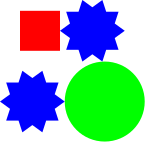
\includegraphics[width=48pt]{elemente/abovebeside.png}|
\end{lstlisting}
%
Für Bilder ist die Signatur \lstinline{image} zuständig; mir ihrer
Hilfe können wir Signaturen für \lstinline{above} und
\lstinline{beside}  formulieren:
%
\begin{lstlisting}
(: beside (image image -> image))
(: above (image image -> image))
\end{lstlisting}
%
An den Signaturen lässt sich klar erkennen, dass es sich um
Kombinatoren handelt.  Indirekt können wir daraus schließen, dass es
in der Datendefinition von Bildern ebenfalls Selbstbezüge gibt.  Die
könnte so aussehen:
%
\begin{lstlisting}
; Ein Bild ist eins der folgenden:
; |\ldots| 
; - eine Nebeneinanderstellung von einem Bild und noch einem Bild
; - eine Übereinanderstellung von einem Bild und noch einem Bild
; |\ldots| 
\end{lstlisting}
%
Das heißt, bei den Bildern ist das gleiche Konstruktionsprinzip am
Werk wie bei den Flüssen: Aus "<kleinen"> Bildern werden "<größere">,
und daraus gegebenenfalls noch größere undsoweiter.

An den Signaturen von \lstinline{beside} und \lstinline{above} ist
leicht erkennbar, dass es sich um Kombinatoren handelt: Es gehen
\lstinline{image} rein und \lstinline{image} kommt auch wieder
heraus.  Um das bei den Flüssen aus dem letzten Abschnitt klar
anzuzeigen, wäre es sinnvoll, für \lstinline{make-confluence}
ebenfalls eine explizite Signatur anzugeben:
%
\begin{lstlisting}
(: make-confluence (string river river -> river))
\end{lstlisting}
%
Kombinatoren verstecken sich in vielen Problemstellungen, Du musst Sie
nur suchen: Dann findest Du erstaunlich oft auch welche.  Darum geht
es in Mantra~\ref{mantra:kombinator}:

\mantrakombinator*

\section{Finanzverträge abbilden}
\label{sec:financial-contracts}

\mentioncode{selbstbezuege/contract.rkt}
%
Es ist Zeit für ein etwas größeres Beispiel.  Wir bilden
Finanzverträge ab und programmieren dazu eine stark vereinfachte
Version eines Klassikers der Informatik-Forschung, das zu mehreren
Veröffentlichungen und zur Gründung einer erfolgreichen Firma geführt
hat.\footnote{Wer mehr wissen möchte, sollte das Paper von Peyton
  Jones und Eber~\cite{FinancialContracts} lesen, das es auch im
  Internet kostenlos zum Download gibt.}  Selbstbezüge spielen eine wichtige
Rolle.

Wichtig bei diesem Beispiel: Für die Repräsentation von
Finanzverträgen aus diesem Abschnitt haben renommierte
Informatik-Forscher mehrere Monate gebraucht.  Wir können sie mit den
bisher präsentierten Programmiermitteln nachbauen, aber Du solltest
nicht von Dir erwarten, dass Du das Beispiel in wenigen Stunden auch
selbst hättest entwickeln können.

In der Finanzbranche werden oft Verträge geschlossen, die zur
strukturierten Zahlung von Geldbeträgen führen.  Wer eine Bankerin
fragt, was der einfachste solche Vertrag ist, bekommt oft die Antwort
\textit{Zero-Bond}.  Hier ist ein Beispiel für einen Zero-Bond:
%
\begin{center}
  Ich bekomme am 31.\ Juni 2030 \EUR{1000}.
\end{center}
%
So ein Vertrag wird immer zwischen zwei Vertragspartnern geschlossen und der
eine ist immer "<ich">.  Daher kommt die Formulierung "<Ich
bekomme">.  Der Begriff "<Zero-Bond"> setzt sich zusammen aus "<keine
Zinsen"> (Zero) und "<Recht auf spätere Zahlung"> (Bond).

Wir können daraus eine einfache Datendefinition machen:
%
\begin{lstlisting}
; Ein Zero-Bond hat folgende Eigenschaften:
; - Datum
; - Betrag
; - Währung
\end{lstlisting}
%
An der Formulierung "<hat folgende Eigenschaften"> sehen wir sofort,
dass es sich um zusammengesetzte Daten handelt.  Daraus folgt direkt
diese Record-Definition:
%
\indexvariable{zero-bond}
\begin{lstlisting}
(define-record zero-bond
  make-zero-bond
  (zero-bond-date     date)
  (zero-bond-amount   rational)
  (zero-bond-currency currency))
\end{lstlisting}
%
Wir müssten noch Definitionen für \texttt{date} und \texttt{currency}
beisteuern, schieben das aber auf die lange Bank.  Wir wollen
stattdessen zunächst noch einmal grundsätzlich über die richtige
Datendefinition für solche Verträge nachdenken.

Es gibt ja noch viel mehr solche Verträge: Futures, Forwards, Swaps,
Swaptions~\ldots{} Jeder Vertrag hat mehrere Eigenschaften, das würde
also darauf hinauslaufen, dass wir sehr viele Datendefinitionen für
zusammengesetzte Daten und die zugehörigen Record-Definitionen
schreiben müssten~-- und am Ende eine Datendefinition zu "<Vertrag">,
die auf eine große Signatur für gemischte Daten hinausläuft.  Das ist
eine Menge Arbeit, und sie wäre auch nie fertig, weil sich die Banker
ständig neue Verträge ausdenken.

Wer aber genug solche Verträge studiert, bemerkt, dass diese aus
Bausteinen bestehen, die immer wiederkehren.  Das suggeriert einen
anderen Ansatz, nämlich diese Bausteine zu identifizieren und dafür
die Datenanalyse durchzuführen.  Wir vollziehen stattdessen die
Arbeit der Autoren des Papers~\cite{FinancialContracts} nach.  Die haben
(über mehrere Monate) einen Satz bestechend einfacher Bausteine
zusammengestellt, indem sie bekannte Verträge in möglichst kleine und
einfache Bestandteile zerlegten.  Jeder dieser Bestandteile ist für
sich genommen ein "<kleiner Vertrag">, es gibt aber auch Kombinatoren,
die aus kleinen Verträgen größere machen, insbesondere auch noch
unbekannte Klassen von Verträgen.  Mit diesen Bestandteilen lassen sich
durch den Einsatz von Kombinatoren sehr viele Finanzverträge (auch
noch unbekannte) abbilden.

Da es mehrere Klassen von Bausteinen und Kombinatoren gibt, werden wir
Verträge als gemischte Daten repräsentieren und dafür schrittweise
eine Datendefinition aufbauen:
%
\begin{lstlisting}
; Ein Vertrag ist eins der folgenden:
; - ...
\end{lstlisting}
%
Dazu gehört natürlich eine passende Signatur-Definition, die wir
ebenfalls schrittweise aufbauen werden:
%
\begin{lstlisting}
(define contract
  (signature (mixed |\ldots|)))
\end{lstlisting}
%
Um die Bausteine und Kombinatoren zu identifizieren, schauen wir uns
zunächst den Zero-Bond näher an.  Auch wenn der einfach aussieht, gibt
es mehrere Aspekte, die auch unabhängig voneinander Sinn ergeben: die
Auszahlung eines bestimmten \textit{Betrags} in einer bestimmten
\textit{Währung} und die Möglichkeit, eine Zahlung \textit{später} zu
veranlassen.  Das sind drei separate Ideen, und es ist sinnvoll, diese
getrennt als Daten zu repräsentieren.

\paragraph{Zahlung einer bestimmten Währung}
Fangen wir an mit der Zahlung einer bestimmten Währung.  Der
Einfachheit halber nehmen wir an, dass alle Zahlungen in Euro sind.
Um die richtige Daten-Definition zu finden, versuchen wir, die
\emph{einfachste} Euro-Zahlung zu finden, und die besteht aus
\emph{einem} Euro.  Die Daten-Definition dazu ist ernüchternd einfach:
%
\begin{lstlisting}
; Ein Euro hat keine Eigenschaften
\end{lstlisting}
%
Wir könnten den Euro einfach als die Zeichenkette \lstinline{"EUR"}
abbilden.  Das wäre sinnvoll, wenn der Euro Teil einer Aufzählung ist.
Dies ist allerdings hier nicht der Fall, andere Vertragsbausteine haben
durchaus Eigenschaften.  (Siehe dazu auch
Aufgabe~\ref{aufgabe:aufzaehlung-vs-nullstellig} auf
Seite~\pageref{aufgabe:aufzaehlung-vs-nullstellig}.)  Wir nehmen die
Datendefinition stattdessen beim Wort "<hat~\ldots{} Eigenschaften">
und bilden den Euro als zusammengesetzte Daten ab.  Dann wird daraus
folgende Record-Definition:
%
\indexvariable{one-euro}
\begin{lstlisting}
(define-record one-euro
  make-one-euro
  one-euro?)
\end{lstlisting}
%
Wir fügen als Nächstes \lstinline{one-euro} zur Daten- und zur
Signatur-Definition von \lstinline{contract} hinzu:
%
\begin{lstlisting}
; Ein Vertrag ist eins der folgenden:
; - ein Euro
; - ...
(define contract
  (signature (mixed one-euro |\ldots|)))
\end{lstlisting}
%
\paragraph{Beliebige Beträge}
Als Nächstes bilden wir die Möglichkeit ab, einen Betrag zu wählen.
Eine naheliegende erste Idee wäre, die Idee "<$n$ Euros"> abzubilden,
etwa so:
%
\indexvariable{euros}
\begin{lstlisting}
; Euros haben folgende Eigenschaft:
; - wieviele
(define-record euros
  make-euros
  euros?
  (euros-amount rational))
\end{lstlisting}
%
Wenn wir das hätten, bräuchten wir aber \lstinline{one-euro} nicht mehr.
Außerdem wäre das Resultat dann nicht mehr so einfach wie möglich:
Besser wäre es, wenn wir die Idee "<wieviele"> trennen könnten von
"<Euro">.  Dann könnten wir sagen "<eine Vielzahl von einem Euro">.  Das
klingt erstmal komisch: %, auch in der Datendefinition:
%%%% HK: "Mehrere haben folgende Eigenschaften klingt mir dann doch zu blöd
%
\begin{lstlisting}
; Eine Vielzahl hat folgende Eigenschaften:
; - wieviele
; - wovon
\end{lstlisting}
%
Aber die richtige Form für zusammengesetzte Daten hat das schon
einmal.  Es reicht für eine erste Skizze einer Record-Definition:
%
\begin{lstlisting}
(define-record multiple
  make-multiple
  multiple?
  (multiple-number |\ldots|)
  (multiple-of     |\ldots|))
\end{lstlisting}
%
Wir müssen aber noch klären, was die Signatur von
\lstinline{multiple-number} respektive \lstinline{multiple-of} ist.
Bei \lstinline{multiple-number} müssen wir uns nicht auf ganze Zahlen
beschränken~-- ein halber Euro geht schließlich auch.  Da ist
\lstinline{rational} sinnvoll.

Bei \lstinline{multiple-of} liegt es nahe, \lstinline{one-euro}
hinzuschreiben: Dann könnten wir den Zero-Bond schon hinschreiben.
Allerdings wäre \lstinline{multiple} ziemlich eingeschränkt und nicht
besonders zukunftssicher: Was, wenn andere Währungen dazukommen,
\lstinline{one-gbp} oder so?  Vielleicht sind wir versucht, eine
Signatur \lstinline{currency} für Währungen zu definieren und für
\lstinline{multiple-of} zu verwenden.  Aber das wäre immer noch zu
eingeschränkt: Man kann ja auch mehrere Aktien (zum Beispiel) im
Rahmen eines Vertrags übergeben~-- oder auch mehrere Zero-Bonds oder
andere Verträge.

Und da ist sie ganz plötzlich, die zentrale Idee: Dass ein Vertrag den
Abschluss \emph{anderer} Ver\-träge verfügen kann.  Wir schreiben
deshalb als Signatur von \lstinline{multiple-of} einfach
\lstinline{contract} und schärfen bei der Gelegenheit die Datendefinition:
%
\indexvariable{multiple}
\begin{lstlisting}
; Ein Vielfaches besteht aus:
; - Anzahl
; - Vertrag 
(define-record multiple
    make-multiple
    multiple?
    (multiple-number rational)
    (multiple-of     contract))
\end{lstlisting}
%
Nun gibt es schon zwei Klassen von Verträgen~-- \lstinline{one-euro} und
\lstinline{multiple}.  Wir erweitern die Definition von
\lstinline{contract} entsprechend:
%
\begin{lstlisting}
(define contract
  (signature (mixed one-euro multiple)))
\end{lstlisting}
%
Mit Hilfe von \lstinline{one-euro} und \lstinline{multiple} können wir
einen Vertrag definieren, der festlegt, dass wir \EUR{100} bekommen~--
sofort:
%
\begin{lstlisting}
(define euro100 (make-multiple 100 (make-one-euro))) ; 100 Euros
\end{lstlisting}
%
\begin{aufgabeinline}
  Definiere eine Funktion \lstinline{make-euros} mit Kurzbeschreibung,
  Signatur und Test wie folgt:
\begin{lstlisting}
; Euro-Betrag auszahlen
(: make-euros (rational -> contract))

(check-expect (make-euros 100) euro100)
\end{lstlisting}
\end{aufgabeinline}
%
Mit Hilfe der Funktion aus der Aufgabe können wir leicht auch
\EUR{200} definieren:
%
\begin{lstlisting}
(define euro200 (make-euros 200)) ; 200 Euros
\end{lstlisting}

\paragraph{Verzögerungen}
Für die Zero-Bonds benötigen wir noch die Möglichkeit,
eine Zahlung zu verzögern.
Dazu benutzen wir den gleichen Trick wie
bei \lstinline{multiple} und definieren einen weiteren Kombinator, der
einen ganzen Vertrag verzögert: Wir schließen also einen Vertrag ab,
später einen Vertrag abzuschließen, und der kann dann die Zahlung
auslösen.  Um so einen Vertrag zu beschreiben, benötigen wir das
Datum, an dem der "<spätere"> Vertrag aktiv wird und den späteren
Vertrag selbst:
%
\begin{lstlisting}
; Eine Verzögerung besteht aus:
; - Datum
; - Vertrag, der zu dem Datum gültig wird
\end{lstlisting}
%
Diese Datendefinition beschreibt wieder zusammengesetzte Daten.  Die
dazugehörige Record"=Definition sieht so aus:
%
\indexvariable{later}
\begin{lstlisting}
(define-record later
  make-later
  later?
  (later-date     date)
  (later-contract contract))
\end{lstlisting}
%
Mit \lstinline{later} können wir die Signatur-Definition von
\lstinline{contract} erweitern:
%
\begin{lstlisting}
(define contract
  (signature (mixed one-euro multiple later)))
\end{lstlisting}
%
Aber es fehlt noch etwas: Wir haben für \lstinline{later-date} die
Signatur \lstinline{date} verwendet, die noch gar nicht definiert ist.
Ein Datum besteht aus Jahr, Monat und Tag, was direkt zu einer
Record-Definition führt:
%
\indexvariable{date}
\begin{lstlisting}
(define-record date
  make-date
  date?
  (date-year  natural)
  (date-month natural)
  (date-day   natural))
\end{lstlisting}
%
\begin{aufgabeinline}
  Wir haben für alle Felder von \lstinline{date} die Signatur
  \lstinline{natural} verwendet. Diese Signatur ist sehr unpräzise,
  zumindest für \lstinline{date-month} und \lstinline{date-day}.

  Verbessere die Signaturen von \lstinline{date-month} und
  \lstinline{date-day} mit Hilfe von \lstinline{integer-from-to}
  aus Abschnitt~\ref{function:integer-from-to} auf
  Seite~\pageref{function:integer-from-to}!
\end{aufgabeinline}
%
Bevor es weitergeht, definieren wir noch zwei Beispiele für das Datum:
%
\begin{lstlisting}
(define date1 (make-date 2019 07 26)) ; 26. Juli 2019
(define date2 (make-date 2019 12 24)) ; Weihnachten 2019
\end{lstlisting}
%
Mit Hilfe dieser Definitionen können wir auch endlich zwei Beispiele
für \lstinline{later} angeben:
%
\begin{lstlisting}
(define later1
  (make-later date1 euro100)) ; Ich bekomme am 26.7.2019 100|\EUR{}|.
(define later2
  (make-later date2 euro200)) ; Ich bekomme Weihnachten 2019 200|\EUR{}|.
\end{lstlisting}
%
Außerdem können wir den Zero-Bond vom Anfang dieses Abschnitts
definieren:
%
\begin{lstlisting}
; Ich bekomme am 31. Juni 2030 1000|\EUR{}|.
(define zero1 (make-later (make-date 2030 06 31)
                          (make-euros 1000)))
\end{lstlisting}

\begin{figure}[tb]
  \centering
\begin{tikzpicture}
  \draw [fill=gray!50] (0, 0) rectangle (10, 4);
  \draw [fill=gray!75] (0.5, 0.5) rectangle (9.5, 3);
  \draw [fill=gray] (1, 1) rectangle (8, 2);
  \node [right] at (0.5, 3.5) {\lstinline{later}};
  \node at (5, 3.5) {\lstinline{"31.6.20230"}};
  \node [right] at (1, 2.5) {\lstinline{multiple}};
  \node at (5, 2.5) {\lstinline{1000}};
  \node [right] at (1.5, 1.5) {\lstinline{one-euro}};
\end{tikzpicture}
  
  \caption{Zero-Bond als Schichten dargestellt}
  \label{fig:zero-bond}
\end{figure}

\noindent Abbildung~\ref{fig:zero-bond} zeigt den Aufbau des
Zero-Bonds \lstinline{zero1} als ineinandergeschachtelte Schichten:
In den \lstinline{later}-Vertrag ist ein \lstinline{multiple}-Vertrag
eingeschachtelt, und dort wiederum der \lstinline{one-euro}-Vertrag.
Aus dieser Sicht ist der \lstinline{multiple}-Vertrag der
"<innere"> Vertrag des \lstinline{later}-Vertrags.

\paragraph{Verträge kombinieren}

Jetzt wo die Zero-Bonds erledigt sind, können wir überlegen, ob es
noch weitere Möglichkeiten geben sollte, Verträge herzustellen.  Immer
wenn Du Repräsentationen mit Kombinatoren baust, solltest Du nach
Möglichkeiten suchen, aus zwei Dingen ein größeres Ding zu bauen.

Beispiele für dieses Prinzip haben wir in diesem Kapitel schon mehrere
gesehen:
%
\begin{itemize}
\item Ein Hauptfluss und ein Nebenfluss werden zu einem Fluss
  kombiniert.
\item Zwei Bilder werden übereinander, nebeneinander und aufeinander
  zu einem Bild kombiniert.
\end{itemize}
%
Auf die Verträge bezogen bedeutet dies, dass wir zwei Verträge
zu einem zusammensetzen, der die Rechte und Pflichten von beiden kombiniert.
So könnte dies gehen:
%
\begin{lstlisting}
; Eine Kombinationsvertrag besteht aus:
; - Vertrag Nr. 1
; - Vertrag Nr. 2
\end{lstlisting}
%
Das sind wieder zusammengesetzte Daten mit zwei Selbstbezügen:
%
\indexvariable{both}
\begin{lstlisting}
(define-record both
  make-both
  both?
  (both-contract-1 contract)
  (both-contract-2 contract))
\end{lstlisting}
%
Hier sind zwei Beispiele für \lstinline{both}:
%
\begin{lstlisting}
; Heute 100|\EUR{}|, später nochmal 100|\EUR{}|
(define both1 (make-both euro100 later1))
; Heute 200|\EUR{}|, später nochmal 200|\EUR{}|
(define both2 (make-both both1 later2))
\end{lstlisting}
%
Wir müssen noch die Definition von \lstinline{contract} erweitern:
%
\begin{lstlisting}
(define contract
  (signature (mixed one-euro multiple later both)))
\end{lstlisting}
%

\paragraph{Der kleinste Vertrag}

Es gibt noch ein weiteres Prinzip beim Repräsentieren mit
Kombinatoren: Suche immer nach dem \emph{kleinsten} möglichen
Baustein.  Wir haben ja schon einen ziemlich kleinen Baustein
definiert: \lstinline{one-euro}.  Aber oft ist der kleine Baustein
eine Variation von "<nichts">, und so ist es auch hier: Der kleinste
Vertrag ist einer ohne Rechte oder Pflichten.  Ihn sollten wir
unbedingt auch definieren~-- zunächst nur der Vollständigkeit halber,
aber später werden wir ihn tatsächlich noch brauchen.

Solch ein "<Nichts-Vertrag"> hat, wie \lstinline{one-euro} auch, keine
Eigenschaften.  Wir repräsentieren ihn aber, genau wie bei
\lstinline{one-euro}, durch einen Record, damit wir ihn mit Hilfe
seiner Signatur in die Definition von \lstinline{contract} einbauen
können:
%
\indexvariable{nothing}
\begin{lstlisting}
; Ein Nichts-Vertrag hat keine Eigenschaften
(define-record nothing
  make-nothing
  nothing?)
\end{lstlisting}
%
Entsprechend erweitern wir \lstinline{contract}:
%
\indexvariable{contract}
\begin{lstlisting}
(define contract
  (signature
   (mixed one-euro multiple later both nothing)))
\end{lstlisting}
%
In Aufgabe~\ref{aufgabe:give} auf Seite~\pageref{aufgabe:give} geht es
um noch einen weiteren Kombinator.

\paragraph{Verträge bewerten}

Wir haben viel Energie für die Repräsentation von Verträgen verwendet,
aber noch gar nichts damit gemacht.  Es fehlen noch ein paar saftige
Funktionen!

Wenn wir einen Vertrag haben, wollen wir vielleicht wissen, wieviel
Geld wir eigentlich insgesamt bekommen.  Das nehmen wir uns als erste
%% HK 2020-01-27: "jetzt" würde heissen "jetzt", also zu "diesem"
%% Zeitpunkt, das ist sicher nicht gemeint
Aufgabe vor.  Wir fangen an mit folgender Kurzbeschreibung:
%
\begin{lstlisting}
; Für einen Vertrag berechnen, wieviel Geld wir bekommen
\end{lstlisting}
%
In der Kurzbeschreibung tauchen die Begriffe "<Vertrag"> und "<Geld">
auf, das übersetzen wir in folgende Signatur:
%
\begin{lstlisting}
(: contract-payment (contract -> rational))
\end{lstlisting}
%
Die Funktion fasst alle Zahlungen zu einem Euro-Betrag zusammen,
Zinsen ignorieren wir.  Die Funktionsweise illustrieren wir wie immer
mit Testfällen.  Bei festen Euro-Beträgen ist recht klar, was
herauskommen muss:
%
\begin{lstlisting}
(check-expect (contract-payment euro100) 100)
(check-expect (contract-payment euro200) 200)
\end{lstlisting}
%
Die Beispiele \lstinline{later1} und \lstinline{later2} sind
verzögerte Verträge über \EUR{100} beziehungsweise \EUR{200}.  Die
Verzögerung spielt bei \lstinline{contract-payment} keine Rolle:
%
\begin{lstlisting}
(check-expect (contract-payment later1) 100)
(check-expect (contract-payment later2) 200)
\end{lstlisting}
%
Bei den beiden \lstinline{both}-Beispielen werden jeweils zwei
Zahlungen von \EUR{100} respektive \EUR{200} kombiniert:
%
\begin{lstlisting}
(check-expect (contract-payment both1) 200)
(check-expect (contract-payment both2) 400)
\end{lstlisting}
%
Die Schablone sieht so aus:
%
\begin{lstlisting}
(define contract-payment
  (lambda (contract)
    |\ldots|))
\end{lstlisting}
%
Da es sich bei der Definition von \lstinline{contract} um gemischte
Daten handelt, sieht die erste Schablone für
\lstinline{contract-payment} so aus:
%
\begin{lstlisting}
(define contract-payment
  (lambda (contract)
    (cond
      ((nothing? contract) |\ldots|)
      ((one-euro? contract) |\ldots|)
      ((multiple? contract) |\ldots|)
      ((later? contract) |\ldots|)
      ((both? contract) |\ldots|))))
\end{lstlisting}
%
Bei den einzelnen Fällen von \lstinline{contract} handelt es sich
jeweils um zusammengesetzte Daten, wir können also die Schablone um
die Anwendungen der Selektoren ergänzen, soweit es welche gibt:
%
\begin{lstlisting}
(define contract-payment
  (lambda (contract)
    (cond
      ((nothing? contract) |\ldots|)
      ((one-euro? contract) |\ldots|)
      ((multiple? contract)
       |\ldots|
       (multiple-number contract)
       (multiple-of contract)
       |\ldots|)
      ((later? contract)
       |\ldots|
       (later-date contract)
       (later-contract contract)
       |\ldots|)
      ((both? contract)
       |\ldots|
       (both-contract-1 contract)
       (both-contract-2 contract)
       |\ldots|))))
\end{lstlisting}
%
Es geht noch weiter:\\
\lstinline{(multiple-of contract)},\\
\lstinline{(later-contract contract)},\\
\lstinline{(both-contract-1 contract)}  und \lstinline{(both-contract-2 contract)} \\
sind allesamt
Selbstbezüge, wir können also dort rekursive Aufrufe hinschreiben:
%
\begin{lstlisting}
(define contract-payment
  (lambda (contract)
    (cond
      ((nothing? contract) |\ldots|)
      ((one-euro? contract) |\ldots|)
      ((multiple? contract)
       |\ldots|
       (multiple-number contract)
       (contract-payment (multiple-of contract))
       |\ldots|)
      ((later? contract)
       |\ldots|
       (later-date contract)
       (contract-payment (later-contract contract))
       |\ldots|)
      ((both? contract)
       |\ldots|
       (contract-payment (both-contract-1 contract))
       (contract-payment (both-contract-2 contract))
       |\ldots|))))
\end{lstlisting}
%
Damit ist die Schablone fertig und wir können versuchen, für jeden Fall
etwas Sinnvolles hinzuschreiben.  Bei den ersten beiden ist es nicht
so schwierig: Bei einem \lstinline{nothing}-Vertrag wird nichts
ausgezahlt, bei einem \lstinline{one-euro}-Vertrag wird ein \EUR{1}
ausgezahlt:
%
\begin{lstlisting}
(define contract-payment
  (lambda (contract)
    (cond
      ((nothing? contract) 0)
      ((one-euro? contract) 1)
      |\ldots|)))
\end{lstlisting}
%
Wir nehmen uns als Nächstes den \lstinline{multiple}-Fall vor: Da
stehen in der Schablone schon:
\begin{itemize}
\item\lstinline{(multiple-number contract)}, also die \emph{Anzahl}
\item\lstinline{(contract-payment (multiple-of contract))}, also
  \emph{was bei einem ausgezahlt} wird
\end{itemize}
% 
Diese beiden Grüßen müssen wir miteinander multiplizieren, um die
Gesamtsumme zu berechnen, die ausgezahlt wird:
%
\begin{lstlisting}
(define contract-payment
  (lambda (contract)
    (cond
      |\ldots|
      ((multiple? contract)
       (* (multiple-number contract)
          (contract-payment (multiple-of contract))))
      |\ldots|)))
\end{lstlisting}
%
Nun ist der \texttt{later}-Fall an der Reihe.  Für
\lstinline{contract-payment} ist \lstinline{(later-date contract)},
also der Zeitpunkt, zu dem der Vertrag aktiv wird, irrelevant: Es geht
ja nur um den Betrag des "<inneren"> Vertrags, und der steht schon in
der Schablone:
%
\begin{lstlisting}
(define contract-payment
  (lambda (contract)
    (cond
      |\ldots|
      ((later? contract)
       (contract-payment (later-contract contract)))
      |\ldots|)))
\end{lstlisting}
%
Zu guter letzt kommt \lstinline{both}.  Die Zahlungen, die sich aus
den beiden Teilverträgen ergeben, stehen schon in der Schablone.  Wir
müssen sie lediglich addieren.  Die vollständige Funktion sieht dann
so aus:
%
\indexvariable{contract-payment}
\begin{lstlisting}
(define contract-payment
  (lambda (contract)
    (cond
      ((nothing? contract) 0)
      ((one-euro? contract) 1)
      ((multiple? contract)
       (* (multiple-number contract)
          (contract-payment (multiple-of contract))))
      ((later? contract)
       (contract-payment (later-contract contract)))
      ((both? contract)
       (+ (contract-payment (both-contract-1 contract))
          (contract-payment (both-contract-2 contract)))))))
\end{lstlisting}

\paragraph{Verträge verwalten}

Eine weitere nützliche Funktion von Verträgen betrifft die Entwicklung
eines Vertrags über die Zeit: Je länger ein Vertrag geschlossen ist,
desto mehr Zahlungen werden dadurch getätigt und entsprechend bleiben
weniger Zahlungen übrig.  Um das abzubilden, brauchen wir eine
Funktion, die ausrechnet, was von einem Vertrag nach einem bestimmten
Zeitpunkt noch übrigbleibt.  So könnte die Kurzbeschreibung lauten:
%
\begin{lstlisting}
; Was bleibt übrig, nachdem zu einem gegebenen Datum ausgezahlt wurde?
\end{lstlisting}
%
Um diese Funktion zu schreiben, müssen wir uns erst einmal überlegen,
wie dieser "<Rest"> von einem Vertrag repräsentiert werden kann.  Die
richtige Idee ist so einfach, dass es gar nicht so einfach ist, sie zu
sehen: Den "<Rest eines Vertrags"> können wir wieder als Vertrag
repräsentieren.  Wir müssen also keine neue Datenanalyse durchführen
und können mit der Signatur fortfahren.  Die Funktion braucht als
Eingabe einen Vertrag; als Ausgabe kommt der neue Vertrag heraus.
Außerdem brauchen wir noch das Datum, das in der Kurzbeschreibung
erwähnt wird:
%
\begin{lstlisting}
(: contract-rest (contract date -> contract))
\end{lstlisting}
%
Kommen wir zu einigen Testfällen: Die Verträge \lstinline{euro100} und
\lstinline{euro200} werden sofort ausgezahlt, da bleibt also nichts
mehr übrig:
%
\begin{lstlisting}
(check-expect (contract-rest euro100 date1) (make-nothing))
(check-expect (contract-rest euro200 date1) (make-nothing))
\end{lstlisting}
%
Das Beispiel \lstinline{later1} kommt zum Datum \lstinline{date1} zur
Auszahlung (der 26.~Juli 2019), ab diesem Datum ist also nichts mehr
übrig:
%
\begin{lstlisting}
(check-expect (contract-rest later1 date1) (make-nothing))
\end{lstlisting}
%
Der Beispielvertrag \lstinline{later2} hingegen wird erst zu
\lstinline{date2} ausgezahlt, das ist Weihnachten 2019.\footnote{Als
  dieses Kapitel geschrieben wurde, lag das noch in der Zukunft.}  Zum Zeitpunkt
\lstinline{date1} passiert deswegen noch nichts, der Vertrag
kommt also unverändert zurück:
%
\begin{lstlisting}
(check-expect (contract-rest later2 date1) later2)
\end{lstlisting}
%
Interesant wird es bei den \lstinline{both}-Verträgen.  Bei
\lstinline{both1} passiert der eine Teil sofort, der andere wird
bis \lstinline{date1} verzögert.  Zum Zeitpunkt \lstinline{date1}
bleibt allerdings von beiden Hälften nichts übrig:
%
\begin{lstlisting}
(check-expect (contract-rest both1 date1) (make-nothing))
\end{lstlisting}
%
Bei \lstinline{both2} bleibt allerdings zum Zeitpunkt
\lstinline{date1} noch die "<rechte"> Hälfte übrig
\lstinline{later2}:
%
\begin{lstlisting}
(check-expect (contract-rest both2 date1) later2)
\end{lstlisting}
%
Aber zum Zeitpunkt \lstinline{date2} ist auch das perdu:
%
\begin{lstlisting}
(check-expect (contract-rest both2 date2) (make-nothing))
\end{lstlisting}
%
Wir schreiten nun zur Funktion selbst.  Hier das Gerüst:
%
\begin{lstlisting}
(define contract-rest
  (lambda (contract date)
    |\ldots|))
\end{lstlisting}
%
Die Eingabe-Signatur enthält ein \lstinline{contract}, wir können also
wieder die Schablone für gemischte Daten verwenden:
%
\begin{lstlisting}
(define contract-rest
  (lambda (contract date)
    (cond
      ((nothing? contract) |\ldots|)
      ((one-euro? contract) |\ldots|)
      ((multiple? contract) |\ldots|)
      ((later? contract) |\ldots|)
      ((both? contract) |\ldots|))))
\end{lstlisting}
%
Wir ergänzen als Nächstes die Schablonen für die einzelnen Fälle, bei
denen es sich ja jeweils um zusammengesetzte Daten handelt:
%
\begin{lstlisting}
(define contract-rest
  (lambda (contract date)
    (cond
      ((nothing? contract) |\ldots|)
      ((one-euro? contract) |\ldots|)
      ((multiple? contract)
       |\ldots|
       (multiple-number contract)
       (multiple-of contract)
       |\ldots|)
      ((later? contract)
       |\ldots|
       (later-date contract)
       (later-contract contract)
       |\ldots|)
      ((both? contract)
       |\ldots|
       (both-contract-1 contract)
       (both-contract-2 contract)
       |\ldots|))))
\end{lstlisting}
%
%
Fast hätten wir es vergessen~-- in den Fällen für
\lstinline{multiple}, \lstinline{later} und \lstinline{both} gibt es
ja Selbstreferenzen und damit rekursive Aufrufe:
%
\begin{lstlisting}
(define contract-rest
  (lambda (contract date)
    (cond
      ((nothing? contract) |\ldots|)
      ((one-euro? contract) |\ldots|)
      ((multiple? contract)
       |\ldots|
       (multiple-number contract)
       (contract-rest (multiple-of contract) date)
       |\ldots|)
      ((later? contract)
       |\ldots|
       (later-date contract)
       (contract-rest (later-contract contract) date)
       |\ldots|)
      ((both? contract)
       |\ldots|
       (contract-rest (both-contract-1 contract) date)
       (contract-rest (both-contract-2 contract) date)
       |\ldots|))
    |\ldots|
    (date-year date)
    (date-month date)
    (date-day date)
    |\ldots|))
\end{lstlisting}
%
Wir können außerdem noch die Schablone für \lstinline{date} bemühen,
wobei es sich zum zusammengesetzte Daten handelt.  Das Datum ist nur
im \lstinline{later}-Fall relevant~-- wir füllen die Schablone aus,
wenn wir zu diesem Fall kommen.

Wir fangen wieder mit den einfachen Fällen an.  Bei
\lstinline{nothing} und \lstinline{one-euro} bleibt jeweils nichts
übrig:
%
\begin{lstlisting}
(define contract-rest
  (lambda (contract date)
    (cond
      ((nothing? contract) (make-nothing))
      ((one-euro? contract) (make-nothing))
      |\ldots|)))
\end{lstlisting}
%
\begin{aufgabeinline}
  Sind beide Fälle schon durch Testfälle abgedeckt?  Wenn nicht,
  schreibe einen!
\end{aufgabeinline}
%
Als Nächstes ist \lstinline{multiple} an der Reihe.  Der rekursive
Aufruf aus der Schablone beantwortet die folgende Frage: "<Wieviel ist
von \emph{einem} Vertrag nach dem Datum noch übrig?"> Wenn wir mit $n$
das Ergebnis von \lstinline{(multiple-number contract)} bezeichnen,
dann müssen wir die Frage beantworten, wieviel von $n$
Verträgen übrig bleibt.  Im übertragenen Sinne futtern $n$ Esser in
der Mensa an jeweils der gleichen Portion Brei, werden aber
unterbrochen. Wenn wir wissen, wieviel von einer Portion jeweils übrigbleibt,
wieviel bleibt dann insgesamt übrig?  Wir müssen wieder mit $n$
multiplizieren:
%
\begin{lstlisting}
(define contract-rest
  (lambda (contract date)
    (cond
      |\ldots|
      ((multiple? contract)
       (make-multiple (multiple-number contract)
                      (contract-rest (multiple-of contract) date)))
      |\ldots|)))
\end{lstlisting}
%
Als Nächstes ist der \lstinline{later}-Fall dran.  Der rekursive
Aufruf beantwortet die Frage, was von dem Vertrag übrigbleibt, falls
das Datum \lstinline{date} schon vorbei beziehungsweise gerade heute
ist.  Wenn \lstinline{date} noch in der Zukunft liegt, passiert gar
nichts und die Funktion sollte den gesamten Vertrag
\lstinline{contract} zurückliefern.

Das heißt, das \lstinline{date} in zwei Klassen zerfällt, nämlich (a)
vor oder an dem Datum \lstinline{(later-date contract)} oder (b)
danach.  Wir brauchen also eine Verzweigung danach, und dazu müssen
wir die beiden Daten vergleichen.  Diese Aufgabe ist
kompliziert genug, dass wir sie zurückstellen und uns
vornehmen, später eine Funktion mit folgender Kurzbeschreibung
und Signatur zu schreiben:
%
\begin{lstlisting}
; Ist ein Datum früher als ein anderes?
(: date<=? (date date -> boolean))
\end{lstlisting}
%
Mit Hilfe dieser Funktion können wir den \lstinline{later}-Fall
folgendermaßen fertigstellen:
%
\begin{lstlisting}
(define contract-rest
  (lambda (contract date)
    (cond
      |\ldots|
      ((later? contract)
       (if (date<=? (later-date contract) date)
           (contract-rest (later-contract contract) date)
           contract))
      |\ldots|)))
\end{lstlisting}
%
Wir haben dabei etwas geschummelt und uns darum gedrückt, die
Schablone für \lstinline{date} auszufüllen.  Das müssen wir bei
\lstinline{date<=?} nachholen.

Es bleibt der Fall für \lstinline{both}.  Die rekursiven Aufrufe aus der
Schablone liefern, was vom "<linken"> beziehungsweise "<rechten">
Vertrag übriggeblieben ist.  Wir müssen die Ergebnisse nur wieder
zusammensetzen:
%
\indexvariable{contract-rest}
\begin{lstlisting}
(define contract-rest
  (lambda (contract date)
    (cond
      |\ldots|
      ((both? contract)
       (make-both (contract-rest (both-contract-1 contract) date)
                  (contract-rest (both-contract-2 contract) date))))))
\end{lstlisting}
%
Fertig!

Also fast: Wir müssen ja noch die Funktion \lstinline{date<=?}
schreiben.  Für einen Teil davon spannen wir Dich ein:
%
\begin{aufgabeinline}
  Schreibe ausreichende Testfälle für \lstinline{date<=?}!
\end{aufgabeinline}
%
Hier ist das Gerüst:
%
\begin{lstlisting}
(define date<=?
  (lambda (date1 date2)
    |\ldots|))
\end{lstlisting}    
%
Das es sich sowohl bei \lstinline{date1} als auch \lstinline{date2} um
zusammengesetzte Daten handelt
%
\begin{lstlisting}
(define date<=?
  (lambda (date1 date2)
    |\ldots|
    (date-year date1) (date-year date2)
    (date-month date1) (date-month date2)
    (date-day date1) (date-day date2)
    |\ldots|))
\end{lstlisting}    
%
Um den Rumpf richtig hinzubekommen, müssen wir sorgfältig alle
möglichen Fälle abarbeiten.  Zunächst müssen wir die beiden
Jahreszahlen vergleichen~-- wenn sie bei \lstinline{date1} und
\lstinline{date2} unterschiedlich sind, so steht das Ergebnis fest.
Wenn nicht, so muss die Funktion die Monate vergleichen und
schließlich die Tage.  Das sieht am Ende so aus:
%
\indexvariable{date<=?}
\begin{lstlisting}
(define date<=?
  (lambda (date1 date2)
    (cond
      ((< (date-year date1) (date-year date2)) #t)
      ((> (date-year date1) (date-year date2)) #f)
      ((< (date-month date1) (date-month date2)) #t)
      ((> (date-month date1) (date-month date2)) #f)
      ((< (date-day date1) (date-day date2)) #t)
      ((> (date-day date1) (date-day date2)) #f)
      (else #t))))
\end{lstlisting}
    
\paragraph{Verträge vereinfachen}

Leider ist der Code für die \lstinline{contract-rest}-Funktion zwar
vollständig, funktioniert aber nicht wie erwartet: Die Tests schlagen
fehl, und zwar fast alle!  Wie kann das sein?  Hier ist
der erste:
%
\begin{lstlisting}
(check-expect (contract-rest euro100 date1) (make-nothing))
\end{lstlisting}
%
Hier ist die Meldung vom Fehlschlag:
%
\begin{alltt}
Der tatsächliche Wert \textcolor{blue}{#<record:multiple 100 #<record:nothing>>}
ist nicht der erwartete Wert \textcolor{blue}{#<record:nothing>}.
\end{alltt}
%
Was ist passiert?  Zur Erinnerung, der Vertrag \lstinline{euro100} ist
so definiert:
%
\begin{lstlisting}
(define euro100 (make-multiple 100 (make-one-euro))) 
\end{lstlisting}
%
Die \lstinline{contract-rest}-Funktion hat erst einmal berechnet, was
von dem einen Euro übriggeblieben ist und vom Rest dann 100 Stück
zurückgegeben: 100 Stück von nichts.  Das Ergebnis ist ja auch
formal korrekt, aber eben nicht wie vom Testfall erwartet.
Unpraktisch ist es auf jeden Fall:
%
\begin{aufgabeinline}
  Finde noch drei weitere komplizierte Wege, "<Verträge über nichts">
  aufzuschreiben.
\end{aufgabeinline}
%
Um das Problem zu vermeiden, wäre es gut, wenn das Programm Verträge
über "<$n$ mal nichts"> gar nicht erst konstruieren würden.  Dafür
müssen wir beim Konstruktor \lstinline{make-multiple} ansetzen.  Wenn
der auf einen \lstinline{nothing}-Vertrag angewendet wird, muss das
Ergebnis auch wieder ein \lstinline{nothing}-Vertrag sein.  Um das zu
erreichen, müssen wir \lstinline{make-multiple} umdefinieren.  Da die
Definition von \lstinline{make-multiple} von
\lstinline{define-record} erledigt wird, wenden wir einen
Trick an und benennen den Konstruktor erst einmal um, in dem wir die
Record-Definition ändern:
%
\indexvariable{multiple}
\begin{lstlisting}
(define-record multiple
  really-make-multiple
  multiple?
  (multiple-number   rational)
  (multiple-of       contract))
\end{lstlisting}
%
Der Name \lstinline{really-make-multiple} ist reine Konvention~--
solange der Name nur anders ist als \lstinline{make-multiple}!  Als
nächstes definieren wir eine neue Funktion mit dem alten Namen und dem
gleichen Vertrag.  Hier sind Kurzbeschreibung, Signatur und ein Testfall,
der gerade \lstinline{euro100} entspricht:
%
\begin{lstlisting}
; multiple-Vertrag konstruieren, dabei vereinfachen
(: make-multiple (rational contract -> contract))

(check-expect (make-multiple 100 (make-nothing)) (make-nothing))
\end{lstlisting}
%
Hier ist das Gerüst für die Funktion:
%
\indexvariable{make-multiple}
\begin{lstlisting}
(define make-multiple
  (lambda (factor contract)
    |\ldots|))
\end{lstlisting}
%
Die Eingabe \lstinline{contract} zerfällt in zwei Fälle:
\lstinline{nothing} und alle anderen.  Im ersten Fall geben
wir wieder \lstinline{nothing} zurück, im zweiten
rufen wir den richtigen Konstruktor auf:
%
\begin{lstlisting}
(define make-multiple
  (lambda (factor contract)
    (if (nothing? contract)
        (make-nothing)
        (really-make-multiple factor contract))))
\end{lstlisting}
%
Damit funktionieren schonmal die ersten beiden Testfälle, die
ursprünglich fehlgeschlagen sind.  Es bleiben aber noch weitere.  Der erste
ist dieser hier:
%
\begin{alltt}
Der tatsächliche Wert
#<record:both \textcolor{blue}{#<record:nothing> #<record:nothing>>}
ist nicht der erwartete Wert
\textcolor{blue}{#<record:nothing>}.
\end{alltt}
%
Das deutet auf ein analoges Problem wie bei \lstinline{multiple} hin:
Nichts und nochmal nichts ist eben nichts, aber der Konstruktor von
\lstinline{both} weiß das nicht.  Wir wenden den gleichen Trick an und
benennen zunächst den Konstruktor um:
%
\indexvariable{both}
\begin{lstlisting}
(define-record both
  really-make-both
  both?
  (both-contract-1 contract)
  (both-contract-2 contract))  
\end{lstlisting}
%
Als Nächstes definieren wir einen neuen Konstruktor selber:
%
\begin{lstlisting}
; Kombinationsvertrag konstruieren, dabei vereinfachen
(: make-both (contract contract -> contract))

(check-expect (make-both (make-nothing) (make-nothing)) (make-nothing))
\end{lstlisting}
%
Durch diesen Testfall ist "<nichts und nichts"> abgedeckt.  Das können
wir aber noch etwas verallgemeinern.  Das illustrieren am besten die
folgenden Testfälle, bei denen jeweils nur die linke beziehungsweise
rechte Seite des \lstinline{both}-Vertrags nichts ist:
%
\begin{lstlisting}
(check-expect (make-both (make-one-euro) (make-nothing))
              (make-one-euro))

(check-expect (make-both (make-nothing) (make-one-euro)) 
              (make-one-euro))
\end{lstlisting}
%
Hier ist das Gerüst zur Funktion:
%
\begin{lstlisting}
(define make-both
  (lambda (contract-1 contract-2)
    |\ldots|))
\end{lstlisting}
%
Die Eingaben zerfallen in drei Klassen, nämlich wenn
\lstinline{contract-1} nichts ist, wenn \lstinline{contract-2} nichts
ist und alle anderen.  Entsprechend brauchen wir eine Verzweigung mit
drei Zweigen:
%
\indexvariable{make-both}
\begin{lstlisting}
(define make-both
  (lambda (contract-1 contract-2)
    (cond
      ((nothing? contract-1) contract-2)
      ((nothing? contract-2) contract-1)
      (else
       (really-make-both contract-1 contract-2)))))
\end{lstlisting}
%
Und nun endlich verlaufen alle Tests erfolgreich.

Die Funktionen \lstinline{make-multiple} und \lstinline{make-both},
welche die ursprünglichen Konstruktoren gleichen Namens ersetzen und
bei der Konstruktion die entstehenden Verträge gleich schon etwas
vereinfachen heißen auch \textit{smart constructors}.\index{smart constructor}

\paragraph{Kombinatorrepräsentationen finden} Die Autoren des Papers über Finanzverträge
haben Monate gebraucht, um die beschriebene elegante Repräsentation zu
finden.  Sie sind nach zwei Prinzipien vorgegangen, die auch auf viele andere Problemstellungen übertragbar sind.

%
\begin{itemize}
\item Sie haben Finanzverträge in ihre kleinsten Bestandteile zerlegt.
\item Sie haben nach Kombinatoren für Finanzverträge gesucht und
  welche gefunden, entsprechend Mantra~\ref{mantra:kombinator} auf Seite~\pageref{mantra:kombinator}.
\end{itemize}
%

\section*{Aufgaben}

\begin{aufgabe}
  Schreibe Funktionen zum Umgang mit Duschprodukten!
  \begin{enumerate}
  \item Beginne mit zwei verschiedenen Duschprodukten: Seife und
    Shampoo.  Bei Seife ist die Farbe und der pH-Wert relevant, bei
    Shampoo die Farbe und der Haartyp.  Schreibe eine Datendefinition
    für Duschprodukte und den Code dafür!
  \item Füge Duschgel als weiteres Duschprodukt hinzu, das zur Hälfte
    aus einer beliebigen Seife und zur Hälfte aus einem beliebigen
    Shampoo besteht.  (Wir tun einfach so, als wäre das so.)
  \item Füge eine "<Mixtur"> als weiteres Duschprodukt hinzu, das aus
    zwei beliebigen Duschprodukten zusammengerührt wird, mit 
    wählbaren Anteilen für das erste und zweite Duschprodukt.
  \item Schreibe eine Funktion, die den Seifenanteil eines beliebigen
    Duschprodukts berechnet.
  \end{enumerate}
\end{aufgabe}

\begin{aufgabe}
\item Eine geometrische Figur in der zweidimensionalen Ebene ist entweder
%
\begin{itemize}
\item ein \textit{Quadrat} parallel zu den Koordinatenachsen,
\item ein \textit{Kreis}
\item oder eine \textit{Überlagerung} zweier geometrischer Figuren.
  (Die Figuren werden übereinandergelegt; die Flächen der beiden Figuren werden also vereinigt.)
\end{itemize}
%
Führe eine Datenanalyse für geometrische Figuren durch! Schreibe
ein Programm, in dem es möglich ist, geometrische Figuren anzulegen
und zu überprüfen, ob ein gegebener Punkt innerhalb der Fläche einer
gegebenen geometrischen Figur liegt.

Falls Du bei dieser Aufgabe eine Funktion brauchst, die eine
Quadratwurzel zieht (muss nicht zwingend sein), so hat diese den Namen
\lstinline{sqrt}\indexvariable{sqrt} (für "<square root">) und
folgende Signatur:
\begin{lstlisting}
(: sqrt (number -> number))
\end{lstlisting}
\end{aufgabe}

\begin{aufgabe}
  Schreibe einen sinnvollen \textit{smart constructor} für
  \lstinline{later}-Verträge.
\end{aufgabe}

\begin{aufgabe}
  Betrachte folgenden Vertrag:
  %
\begin{lstlisting}
(make-multiple 100 (make-multiple 100 (make-one-euro)))    
\end{lstlisting}
%
Kann dieser Vertrag vereinfacht werden?  Wenn ja, erweitere den
entsprechenden \textit{smart constructor}.
\end{aufgabe}

\begin{aufgabe}\label{aufgabe:give}
  Füge eine weitere Klasse von Verträgen hinzu, die
  \lstinline{give}-Verträge: Ein \lstinline{give}-Vertrag dreht alle
  Zahlungen um, die sich aus einem Vertrag ergeben.  Das heißt, ein
  \lstinline{give}-Vertrag von \EUR{1} führt dazu, dass der
  Vertragsinhaber dem Vertragspartner \EUR{1} \emph{geben} muss und
  nicht bekommt.  Erweitere die beiden Funktionen, so dass sie auch
  mit \lstinline{give}-Verträgen klarkommen.  Benutze, um Zahlungen
  "<in die andere Richtung"> zu repräsentieren, ein negatives
  Vorzeichen.
\end{aufgabe}

\begin{aufgabe}
  Die Funktionen \lstinline{contract-payment} und
  \lstinline{contract-rest} passen nicht so recht zusammen: Die eine
  berechnet \emph{alle} Zahlungen, die anderen den Rest eines Vertrags
  ab einem bestimmten Zeitpunkt.  Schreibe eine Funktion
  \lstinline{contract-payment-until}, die alle Zahlungen bis zu einem
  bestimmten Zeitpunkt berechnet!
\end{aufgabe}

\begin{aufgabe}\label{aufgabe:aufzaehlung-vs-nullstellig}
  Statt nullstelliger zusammengesetzter Daten wie \lstinline{nothing}
  oder \lstinline{one-euro} könnte man theoretisch auch~-- wie bei
  Aufzählungen~-- feste Zeichenketten wie \lstinline{"nothing"} und
  \lstinline{"one-euro"} verwenden.  Versuch dies umzusetzen!
\end{aufgabe}

%%% Local Variables: 
%%% mode: latex
%%% TeX-master: "i1"
%%% End: 




% Diese Datei ist Teil des Buchs "Schreibe Dein Programm!"
% Das Buch ist lizensiert unter der Creative-Commons-Lizenz
% "Namensnennung - Weitergabe unter gleichen Bedingungen 4.0 International (CC BY-SA 4.0)"
% https://creativecommons.org/licenses/by-sa/4.0/deed.de

\chapter{Programmieren mit Listen}
\label{cha:rek}
\label{cha:list}

Im vorigen Kapitel haben wir bereits Daten mit Selbstbezug
kennengelernt, die Informationen variabler Größe repräsentieren
können: Flüsse, Bilder und Finanzverträge.  Die Repräsentationen dafür
waren recht speziell das jeweilige Einsatzgebiet gekoppelt.  In diesem
Kapitel lernen wir eine besonders praktische Datendefinition mit
Selbstbezug kennen, die in nahezu allen Einsatzgebieten nützlich ist:
\textit{Listen}.\index{Liste}

Hier sind einige Listen aus dem täglichen Leben:
%
\begin{center}
  \begin{tabular}{l@{\qquad}l@{\qquad}l@{\qquad}l@{\qquad}l@{\qquad}l}
  Brot & Herbert & 1 & Axl & Dauerwelle & Pumps \\
  Butter & Mike & 2 & Slash & Dreadlocks \\
  Käse & & 3 & Duff & Irokese \\
  & & 4 & Dizzy & Vokuhila \\
  && 5 & Izzy \\
  && 6 & Melissa \\
  &&& Brain\\
  &&& Bumblefoot 
\end{tabular}
\end{center}
%
Keine dieser Listen ist auf ihre jeweilige Länge festgelegt: Zur Liste
mit "<Brot"> könnten beispielsweise noch "<Gurken"> hinzukommen, zur
Liste mit Axl, Slash undsoweiter könnte zum Beispiel noch Steven
dazukommen.

\section{Listen repräsentieren}

\mentioncode{listen/list0.rkt}
%
In der Einführung haben wir Listen mit unterschiedlichen Sorten von
Elementen gesehen.  Für den Anfang konzentrieren wir uns zunächst
einmal auf Listen von Zahlen, um die Dinge einfach zu halten.  Dann
schreiben wir eine Funktion, um die Zahlen aus so einer Liste zu
addieren. Es gibt verschiedene Möglichkeiten, Listen zu
repräsentieren.  Die Repräsentation, die wir in diesem Kapitel
einführen, hat als besonders einfach und universell verwendbar
herausgestellt.

Diese Repräsentation ist nach dem gleichen Prinzip entstanden die zum
Finanzverträge in Abschnitt~\ref{sec:financial-contracts} auf
Seite~\pageref{sec:financial-contracts}: Wir suchen zunächst nach der
einfachsten Liste, die wir uns vorstellen können.  Man könnte auf die
Idee kommen, dass dies eine Liste mit nur einem Element ist, aber noch
einfacher ist eine mit gar keinen Elementen~-- die \textit{leere
  Liste}.\index{leere Liste}\index{Liste!leer}  Natürlich werden
wir auch nichtleere Listen brauchen, darum ist der erste Entwurf
einer Datendefinition wie folgt:
%
\begin{lstlisting}
; Eine Liste aus Zahlen ist eins der folgenden:
; - eine leere Liste
; - eine nichtleere Liste
\end{lstlisting}
%
Die leere Liste hat keine Bestandteile, wir werden sie
aber später von den nichtleeren Listen unterscheiden müssen.  Wir
benutzen deshalb eine leere Record-Definition:
%
\indexvariable{empty-list}
\begin{lstlisting}
; leere Liste
(define-record empty-list
  make-empty-list
  empty?)
\end{lstlisting}
%
Beim Namen für das Prädikat haben wir etwas gemogelt.  Von Amts wegen
müsste es \lstinline{empty-list?} heißen.  Da es aber noch öfter
vorkommen wird, kürzen wir es zu \lstinline{empty?} ab.

Wir definieren außerdem eine Abkürzung für die leere Liste.
Auch diese kommt noch öfter vor, und wir müssen sie so nicht jedesmal
neu komstruieren:
%
\begin{lstlisting}
(define empty (make-empty-list))
\end{lstlisting}
%
Nun sind die nichtleeren Listen dran.  Nach dem Kombinatorprinzip aus dem
vorigen Kapitel sollten wir eine nichtleere Liste konstruieren, indem
wir eine bestehende Liste erweitern:
%
\begin{lstlisting}
; Eine nichtleere Liste besteht aus:
; - dem ersten Element
; - einer Liste aus Zahlen mit den restlichen Elementen
\end{lstlisting}
%
Diese spezielle Definition für nichtleere Listen heißt
\textit{Cons-Liste}.\index{Cons-Liste}  Das zweite Feld enthält
eine "<Liste aus Zahlen">~-- da ist der Selbstbezug.

Wir ändern die Datendefinition für Listen entsprechend ab:
%
\begin{lstlisting}
; Eine Liste aus Zahlen ist eins der folgenden:
; - eine leere Liste
; - eine Cons-Liste

; Eine Cons-Liste besteht aus:
; - dem ersten Element
; - einer Liste aus Zahlen mit den restlichen Elementen
\end{lstlisting}
%
Die Datendefinition für Cons wandeln wir in eine Record-Definition um.
Dafür nehmen wir an, dass die Signatur für Listen von Zahlen
\lstinline{list-of-numbers} heißt~-- die werden wir im Nachgang
definieren:
%
\indexvariable{cons-list}\indexvariable{first}\indexvariable{rest}
\begin{lstlisting}
(define-record cons-list
  cons
  cons?
  (first number)
  (rest  list-of-numbers))
\end{lstlisting}
%
Ähnlich wie bei \lstinline{empty-list} haben wir die Funktionen der
Record-Definition kürzer genannt als sonst, weil sie noch oft
vorkommen werden:
sonst:\indexvariable{cons-list}\indexvariable{cons}\indexvariable{cons?}\indexvariable{first}\indexvariable{rest}\label{def:cons}
Der Konstruktor heißt statt
\lstinline{make-cons-list} hier \lstinline{cons}, das Prädikat nur \lstinline{cons?}  statt
\lstinline{cons-list?} und bei den Selektoren fehlt jeweils das
\lstinline{cons-} vorn.

Es fehlt noch die Definition der Signatur \lstinline{list-of-numbers}
für "<Liste von Zahlen">, die aus leeren Listen und Cons-Listen
gemischt wird:
%
\indexvariable{list-of-numbers}
\begin{lstlisting}
(define list-of-numbers
  (signature
   (mixed empty-list
          cons-list)))
\end{lstlisting}
%
Hier sind einige Beispiele für Listen:
%
\begin{lstlisting}
; leere Liste
(define list0 empty)
; einelementige Liste mit der Zahl 42
(define list1 (cons 42 empty))
; Liste mit den Zahlen 1 2 3
(define list3 (cons 1 (cons 2 (cons 3 empty))))
; Liste mit den Zahlen e und pi
(define list2 (cons 2.7183 (cons 3.14159 empty)))
; Liste mit den Zahlen 2 3 5 7
(define list4 (cons 2 (cons 3 (cons 5 (cons 7 empty)))))
\end{lstlisting}
%
\begin{figure}[tb]
  \centering
  \begin{tikzpicture}
    \draw (0, 0) rectangle (9.5, 4); \node [below] at (1, 4)
    {\lstinline{cons-list}}; \node [right] at (1, 3) {\lstinline{2}};
    \draw (2, 0.5) rectangle (9, 3.5); \node [below] at (3, 3.5)
    {\lstinline{cons-list}}; \node [right] at (3, 2.5)
    {\lstinline{3}}; \draw (4, 1) rectangle (8.5, 3); \node [below] at
    (5, 3) {\lstinline{cons-list}}; \node [right] at (5, 2)
    {\lstinline{5}}; \draw (6, 1.5) rectangle (8, 2.5); \node [right]
    at (6, 2) {\lstinline{empty-list}};
  \end{tikzpicture}
  
  \caption{Struktur der Liste mit den Elementen 2 3 5}
  \label{fig:list-structure}
\end{figure}
%
\noindent An den Beispielen kann man sehen, dass es einen Unterschied
zwischen der intuitiven Struktur von Listen und ihrer Repräsentation
gibt. Intuitiv besteht eine Liste aus einer Aneinanderreihung ihrer
Elemente.  Die Repräsentation ist aber geschachtelt, wie
Abbildung~\ref{fig:list-structure} zeigt.  Sie erlaubt uns
insbesondere, aus kleineren Listen größere zu bauen und trotzdem die
kleineren Listen wiederzuverwenden:
%
\begin{lstlisting}
; Liste mit den Zahlen 1 2 3 5 7
(define list5 (cons 1 list4))
\end{lstlisting}
%
Dieses Beispiel zeigt außerdem, dass der Konstruktor \lstinline{cons} an eine
existierende Liste \emph{vorn} ein Element anhängt.

\label{sec:list-sum}
Nun sind wir bereit, eine Funktion über Listen zu schreiben, welche
die Zahlen einer Liste aufaddiert.  Kurzbeschreibung und Signatur
sehen so aus:
%
\begin{lstlisting}
; Summe der Elemente einer Liste von Zahlen berechnen
(: list-sum (list-of-numbers -> number))
\end{lstlisting}
%
Als Nächstes brauchen wir Testfälle, die wir mit Hilfe der
Beispiel-Listen von oben (und gegebenenfalls einem Taschenrechner)
konstruieren:
%
\begin{lstlisting}
(check-expect (list-sum list2) 5.85989)
(check-expect (list-sum list3) 6)
(check-expect (list-sum list4) 17)
\end{lstlisting}
%
\begin{aufgabeinline}
  Schreibe auch Testfälle für \lstinline{list-sum} auf Basis der
  Beispiel-Listen \lstinline{list0} und \lstinline{list1}!  Falls Du
  Dir nicht sicher bist, rate!
\end{aufgabeinline}
%
Als Nächstes kommt wie immer das Gerüst:
%
\begin{lstlisting}
(define list-sum
  (lambda (list)
    |\ldots|))
\end{lstlisting}
%
Die Signatur sagt, dass \lstinline{list-sum} eine Liste als Eingabe
akzeptiert~-- gemischte Daten.  Die Schablone dazu sieht so aus:
%
\begin{lstlisting}
(define list-sum
  (lambda (list)
    (cond
      ((empty? list) |\ldots|)
      ((cons? list) |\ldots|))))
\end{lstlisting}       
%
Beim \lstinline{cons-list}-Fall handelt es sich um zusammengesetzte
Daten, wir können also entsprechend der Schablone dafür
Selektor-Aufrufe hinschreiben.  Bei \lstinline{rest} sitzt außerdem
ein Selbstbezug, wir schreiben also auch einen rekursiven Aufruf in
die Schablone:
%
\begin{lstlisting}
(define list-sum
  (lambda (list)
    (cond
      ((empty? list) |\ldots|)
      ((cons? list)
       |\ldots|
       (first list)
       (list-sum (rest list))
       |\ldots|))))
\end{lstlisting}
%
Nun sind alle möglichen Konstruktionsanleitungen angewendet. Wir
vervollständigen die Schablone, zuerst den Fall für
Cons-Listen.  Dort steht in der Schablone \lstinline{(first list)} 
und \lstinline{(list-sum (rest list))}.  Zum Verständnis
hilft, die beiden Ausdrucke ins Deutsche zu übersetzen:
%
\begin{itemize}
\item \lstinline{(first list)} ist das \emph{erste Element der Liste} und
\item \lstinline{(list-sum (rest list))} ist die \emph{Summe der restlichen
    Elemente}.
\end{itemize}
%
Gefragt
ist aber die Summe \emph{aller Elemente}, dazu müssen wir die beiden
noch addieren:
%
\begin{lstlisting}
(+ (first list) (list-sum (rest list)))
\end{lstlisting}
%
Es bleibt der Fall der leeren Liste.  Intuitiv hat die gar keine
Summe, aber irgendetwas müssen wir da hinschreiben.  Wir schreiben 
vorläufig $0$ ins Programm, werden diese Wahl aber noch diskutieren:
%
\indexvariable{list-sum}
\begin{lstlisting}
(define list-sum
  (lambda (list)
    (cond
      ((empty? list) 0)
      ((cons? list)
       (+ (first list) (list-sum (rest list)))))))
\end{lstlisting}
%
Damit funktionieren die Testfälle und die Funktion ist fertig!

\begin{aufgabeinline}
  Verfolge die Auswertung der Testfälle im Stepper!
\end{aufgabeinline}

\begin{aufgabeinline}
  Ändere den Zweig für die leere Liste und schreibe etwas anderes als
  0 hin.  Funktionieren die Testfälle dann noch?
\end{aufgabeinline}
%
Tatsächlich ist $0$ die einzig richtige Zahl, die im
\lstinline{empty}-Fall stehen darf.  Das mag intuitiv einleuchten: die
leere Liste ist schließlich "<nichts"> und 0 ist auch irgendwie
"<nichts">.  Ein weiteres Beispiel wird aber gleich zeigen, dass diese
Argumentation zu einfach ist.

Wir schreiben als Nächstes eine Funktion, die alle Zahlen einer Liste
\emph{multipliziert}.   Hier sind Kurzbeschreibung, Signatur, Tests
und Gerüst:
%
\begin{lstlisting}
; Produkt der Elemente einer Liste von Zahlen berechnen
(: list-product (list-of-numbers -> number))

(check-expect (list-product list1) 42)
(check-expect (list-product list3) 6)
(check-expect (list-product list4) 210)

(define list-product
  (lambda (list)
    |\ldots|))
\end{lstlisting}
%
Die Schablone entsteht genau wie bei \lstinline{list-sum} aus den
Konstruktionsanleitungen für gemischte Daten, zusammengesetzte Daten
und Selbstbezüge:
%
\begin{lstlisting}
(define list-product
  (lambda (list)
    (cond
      ((empty? list) |\ldots|)
      ((cons? list)
       |\ldots|
       (first list) 
       |\ldots|
       (list-product (rest list))))))
\end{lstlisting}
%
Wir kümmern uns wieder zuerst um den
\lstinline{cons}-Fall. In der Schablone stehen \lstinline{(first list)}, das erste
Element und \lstinline{(list-product (rest list))}, das Produkt der
restlichen Elemente.  Wir müssen nur noch beide miteinander
multiplizieren, um das Produkt aller Elemente zu berechnen:
%
\begin{lstlisting}
(* (first list) (list-product (rest list)))
\end{lstlisting}
%
Bleibt wieder der \lstinline{empty}-Fall~-- wieder die leere Liste.
Die Versuchung ist groß, wieder "<nichts"> hinzuschreiben, also 0.
Dann allerdings schlagen \emph{alle} Testfälle fehl:
\begin{alltt}
Der tatsächliche Wert 0 ist nicht der erwartete Wert 42.
Der tatsächliche Wert 0 ist nicht der erwartete Wert 6.
Der tatsächliche Wert 0 ist nicht der erwartete Wert 210.
\end{alltt}
%
Warum kommt immer $0$ heraus?  Das können wir anhand der Auswertung
von
\lstinline{(list-product list3)}
sehen.  Die sieht so aus~-- wir haben
einige Zwischenschritte ausgelassen:
%
\begin{lstlisting}
(list-product list3)
|\evalsto| (list-product (cons 1 (cons 2 (cons 3 empty))))
|\evalsto| (cond ((empty? (cons 1 |\ldots|)) |\ldots|) ((cons? (cons 1 |\ldots|)) |\ldots|))
|\evalsto| (cond ((empty? (cons 1 |\ldots|)) |\ldots|) ((cons? (cons 1 |\ldots|)) |\ldots|))
|\evalsto| (* (first (cons 1 |\ldots|)) (list-product (rest (cons 1 |\ldots|))))
|\evalsto| (* 1 (list-product (rest (cons 1 |\ldots|))))
|\evalsto| (* 1 (list-product (cons 2 (cons 3 empty))))
|\evalsto| (* 1 (* 2 (list-product (cons 3 empty))))
|\evalsto| (* 1 (* 2 (* 3 (list-product empty))))
|\evalsto| (* 1 (* 2 (* 3 (cond ((empty? empty) 0) |\ldots|))))
|\evalsto| (* 1 (* 2 (* 3 (cond (#t 0) |\ldots|))))
|\evalsto| (* 1 (* 2 (* 3 0)))
\end{lstlisting}
%
Die Auswertung ist auf so einem guten Weg~-- aber um Schluss macht
\lstinline{list-product} alles kaputt und multipliziert mit $0$.  Und so
ist es mit \emph{jeder} Eingabe.  Wir müssten also
statt mit $0$ mit einer Zahl multiplizieren, die das Ergebnis nicht
kaputtmacht sondern genauso lässt, wie es ist.  Im Fall der
Multiplikation ist das die $1$, nicht die $0$.  Die richtige Funktion
sieht damit so aus:
%
\indexvariable{list-product}
\begin{lstlisting}
(define list-product
  (lambda (list)
    (cond
      ((empty? list) 1)
      ((cons? list)
       (* (first list) (list-product (rest list)))))))
\end{lstlisting}
%
Rückblickend können wir damit auch erklären, warum bei
\lstinline{list-sum} im \lstinline{empty}-Fall $0$ stehen muss: Die $0$
macht beim Addieren das Ergebnis nicht kaputt.  Darum spricht man auch
davon, dass $0$ das \textit{neutrale Element}\index{neutrales Element}
bezüglich der Addition ist, $1$ das neutrale Element bezüglich der
Multiplikation.\label{page:neutrales-element}

\section{Listen mit anderen Elementen}

\mentioncode{listen/list-of.rkt}
%
Das Prinzip "<Liste"> ist nicht auf Listen von Zahlen beschränkt:
Genauso gut kann man sich Listen aus Zeichenketten, den Tieren aus
Kapitel~\ref{sec:animal} oder Bildern vorstellen.  Um das zu
ermöglichen, können wir die Datendefinition
anpassen.  Wir entfernen alle Erwähnungen von
Zahlen und sprechen ausschließlich von "<Elementen">:
%
\begin{lstlisting}
; Eine Liste ist eins der folgenden:
; - eine leere Liste
; - eine Cons-Liste

; Eine Cons-Liste besteht aus:
; - dem ersten Element
; - einer Liste mit den restlichen Elementen
\end{lstlisting}
%
Tatsächlich können wir Listen bereits bauen, deren Elemente keine
Zahlen sind:
%
\indexvariable{string-list}
\begin{lstlisting}
(define string-list (cons "Mike" (cons "Sperber" empty)))
\end{lstlisting}
%
\begin{aufgabeinline}
  Probiere die Definition von \lstinline{string-list} aus!
\end{aufgabeinline}
%
Diese Definition kann DrRacket zwar ausführen, aber es gibt jede
Menge Signaturverletzungen.

Die verletzten Signaturen sind allesamt \lstinline{number}, am
prominentesten in der Record-Definition von \lstinline{cons-list}.
Wenn wir dort auch Zeichenketten verwenden wollen, ohne Listen aus
Zahlen zu verbieten, müssen wir über
\lstinline{number} und \lstinline{string} abstrahieren.  Bei der
Record-Definition geht das, indem wir aus \lstinline{cons-list} stattdessen
\lstinline{(cons-list-of element)} machen.
Das wirkt wie ein
\lstinline{lambda} mit \lstinline{element} als Parameter.  Wir können
dann \lstinline{element} innerhalb
der Record-Definition benutzen:\label{function:cons-list-of}
%
\indexvariable{cons-list-of}
\begin{lstlisting}
(define-record (cons-list-of element)
  cons
  cons?
  (first element)
  (rest  |\ldots|))
\end{lstlisting}
%
Diese Record-Definition definiert \lstinline{cons-list-of} als Funktion,
die eine Signatur akzeptiert (die Signatur der Elemente) und eine
Signatur zurückliefert, nämlich die der Cons-Listen mit der gegebenen
Signatur für die Elemente.  Die Signatur können wir auch hinschreiben:
%
\begin{lstlisting}
(: cons-list-of (signature -> signature))
\end{lstlisting}
%
Da \lstinline{cons-list-of} eine Signatur konstruiert, nennen wir diese
Funktion auch \textit{Signatur-Konstruktor}.\index{Signatur-Konstruktor}
Das \lstinline{element} ist ein \textit{Signatur-Parameter}\index{Signatur-Parameter}.
Wir müssen also immer da, wo wir vorher \lstinline{cons-list} stand,
\lstinline{(cons-list-of ...)} schreiben und eine Signatur für die
Elemente angeben, also zum Beispiel \lstinline{(cons-list-of number)}
oder \lstinline{(cons-list-of string)}.

Die Signatur von \lstinline{rest} war vorher
\lstinline{list-of-numbers}, die müssen wir also auch ändern.  Wie
genau, ergibt sich erst im Zusammenhang mit der abstrahierten
Definition von \lstinline{list-of-numbers}.  Da es sich hier um eine
ganz normale Definition mit \lstinline{define} handelt, können wir ein
\lstinline{lambda} benutzen, um über den Signatur der Elemente zu
abstrahieren:
%
\indexvariable{list-of}
\begin{lstlisting}
(define list-of
  (lambda (element)
    (signature
     (mixed empty-list
            (cons-list-of element)))))
\end{lstlisting}
%
Wir können mit dieser Definition nun statt \lstinline{list-of-numbers} also
\lstinline{(list-of number}) schreiben.  Damit können wir auch die
Record-Definition von \lstinline{cons-list-of} vervollständigen, indem
wir beim \lstinline{rest}-Feld als Signatur \lstinline{(list-of element)} schreiben, wo vorher
\lstinline{list-of-numbers} stand:
%
\begin{lstlisting}
(define-record (cons-list-of element)
  cons
  cons?
  (first element)
  (rest  (list-of element)))
\end{lstlisting}
%
Das erledigt die Signaturverletzungen.

\begin{feature}{\texttt{define-record} mit Signatur-Parametern}{scheme:define-record-parameters}
Eine \lstinline{define-record}"=Form\indexvariable{define-record}
mit Signatur-Parametern hat folgende allgemeine Gestalt:\label{def:define-record-parameters}
%
\begin{alltt}
(define-record (\(t\) \(\mathit{sp}\sb{1}\) \(\ldots\) \(\mathit{sp}\sb{k}\))
  \(c\)
  \(p\)
  (\(\mathit{sel}\sb{1}\) \(\mathit{sig}\sb{1}\))
  \(\ldots\)
  (\(\mathit{sel}\sb{n}\) \(\mathit{sig}\sb{n}\)))
\end{alltt}
%
%
\begin{itemize}
\item Die Signatur-Parameter $\mathit{sp}\sb{1} \ldots \mathit{sp}\sb{k}$
können in den Signaturen
\(\mathit{sig}\sb{1}\ldots\mathit{sig}\sb{n}\) verwendet werden.
\item $t$ ist der Name des Signatur-Konstruktors mit der Signatur:
  %
\begin{alltt}
(: \(t\) (signature \(\ldots\) \textrm{(\(k\)-mal)} -> signature))
\end{alltt}
  \item $c$, $p$ und $\mathit{sel}_1, \ldots, \mathit{sel}_n$ sind 
    die Namen von Konstruktor, Prädikat und Selektoren.
\end{itemize}
%
\end{feature}

Abbildung~\ref{scheme:define-record-parameters} fasst die
neue Form von \lstinline{define-record} mit
Signatur-Parametern zusammen.
Bei dieser neuen Form von \lstinline{define-record} ist
nicht mehr offensichtlich, wie die Signaturen des Konstruktors und der
beiden Selektoren aussehen sollen, wenn wir sie ausschreiben.  Wir
brauchen dafür ein neues Konstrukt, um auszudrücken, dass potenziell
bei jedem Aufruf von \lstinline{cons}, \lstinline{first} und
\lstinline{rest} eine andere Elementsignatur verwendet wird.  Das
sieht so aus:
%
\begin{lstlisting}
(: cons (%element (list-of %element) -> (cons-list-of %element)))
(: first ((cons-list-of %element) -> %element))
(: rest ((cons-list-of %element) -> (list-of %element)))
\end{lstlisting}
%
Das \verb|%| kennzeichnet
\textit{Signaturvariablen}\index{Signaturvariable}.  Die
Signaturvariable \lstinline{%element} steht für eine beliebige
Signatur.  Die Signatur-Deklaration von \lstinline{cons} bedeutet
außerdem, dass die Signatur von neuem Element (das erste \lstinline{%element})
und die Signatur der Listenelemente (das \lstinline{%element} in 
\lstinline{(list %element)} übereinstimmen sollten.  (DrRacket
  überprüft dies aber nicht.)

Vielleicht ist Dir der Gedanke gekommen, dass statt
\lstinline{%element} in den obigen Signaturen auch \lstinline{any}
stehen könnte.  Rein technisch gesehen ist das korrekt.  Allerdings
wären die resultierenden Signaturen weniger präzise.  Nimm einmal
an, dort stünde zum Beispiel das hier:
%
\begin{lstlisting}
(: cons (any (list-of any) -> (cons-list-of any)))
\end{lstlisting}
%
Diese Signatur sagt "<\lstinline{cons} akzeptiert irgendeinen Wert und
irgendeine Liste und produziert wieder irgendeine Liste">.  Zum
Vergleich sagt die Signatur
%
\begin{lstlisting}
(: cons (%element (list-of %element) -> (cons-list-of %element)))
\end{lstlisting}
%
aus, dass das neue Element, das \lstinline{cons} akzeptiert, die
gleiche Signatur erfüllen muss wie die schon vorhandenen Elemente der
Liste und die Elemente der Resultatliste: Alle drei Vorkommen von \lstinline{%element} müssen in einer
konkreten Anwendung von \lstinline{cons} die gleiche Signatur sein.

Bevor das Programm wieder
funktioniert, müssen wir noch ein kleines Problem
beheben:

\lstinline{List-of-numbers} ist nicht mehr
definiert, steht aber noch in den Signatur"=Deklarationen von
\lstinline{list-sum} und \lstinline{list-product}.  Wir können
entweder \lstinline{list-of-numbers} durch \lstinline{(list-of number)}
ersetzen oder eine Signatur-Definition
dazuschreiben:
%
\indexvariable{list-of-numbers}
\begin{lstlisting}
(define list-of-numbers (signature (list-of number)))
\end{lstlisting}
%
Diese Definition muss vor \lstinline{list-sum}
und \lstinline{list-product} stehen, damit sie dort bekannt ist.

\section{Konstruktionsanleitung}

Bei der Konstruktion von Funktionen, die Listen akzeptieren, haben wir
drei Schablonen kombiniert: gemischte und
zusammengesetzte Daten sowie Selbstbezüge.  Wir
werden noch viele Funktionen mit Listen als Eingabe schreiben.
Deshalb lohnt es sich, solchen Funktionen eine eigene
Konstruktionsanleitung zu widmen:

\begin{konstruktionsanleitung}{Listen als Eingabe: Schablone}
  \label{ka:listen-eingabe-schablone}
Die Schablone für eine Funktion, die eine Liste akzeptiert, sieht
folgendermaßen aus:
%
\begin{lstlisting}
(: |\(f\)| (... (list-of |\(\mathit{elem}\)|) ... -> ...))

(define |\(f\)|
  (lambda (|\ldots| |\(\mathit{list}\)| |\ldots|)
    (cond
      ((empty? |\(\mathit{list}\)|) |\ldots|)
      ((cons? |\(\mathit{list}\)|)
       |\ldots|
       (first |\(\mathit{list}\)|)
       |\ldots|
       (|\(f\)| |\ldots| (rest |\(\mathit{list}\)|) |\ldots|)
       |\ldots|
       ))))
\end{lstlisting}
  
  
\end{konstruktionsanleitung}

\section{Eingebaute Listen}

Da Listen in diesem Buch noch oft vorkommen und es umständlich ist,
jedesmal die Definitionen für \lstinline{cons} und \lstinline{list-of} an
den Anfang von Programmen zu setzen, macht die nächste Sprachebene das
Programmieren mit Listen einfacher.\index{Sprachebene}

\smallskip

\noindent\textbf{Schalte deshalb in die nächste Sprachebene hoch:}

\smallskip

\noindent Fange eine neue Datei an.  Wähle danach wieder das Menü
\texttt{Sprache} aus, darunter den Menüpunkt \texttt{Sprache auswählen} und dann
\texttt{Schreibe Dein Programm!} (\emph{ohne} \texttt{Anfänger}).
Dann drücke noch einmal \texttt{Start}.

\begin{feature}{\texttt{list}}{scheme:list}
  Die eingebaute Funktion \lstinline{list}\indexvariable{list} erlaubt es, Listen aus ihren Elementen
  ohne Verwendung von \lstinline{cons} zu erzeugen.  Sie
  akzeptiert eine beliebige Anzahl von Argumenten, macht daraus eine
  Liste und gibt diese zurück:
%
\begin{lstlisting}
(list 1 2 3)
|\evalsto| #<list 1 2 3>
(list "Axl" "Slash" "Izzy")
|\evalsto| #<list "Axl" "Slash" "Izzy">
\end{lstlisting}
\end{feature}

Ab sofort sind \lstinline{cons}, \lstinline{cons?}, \lstinline{first} und
\lstinline{rest} vordefiniert genau wie der Signaturkonstruktor
\lstinline{list-of}.  Es gibt außerdem eine praktische neue Funktion
\lstinline{list}, die in Abbildung~\ref{scheme:list} beschrieben ist.

In der neuen Sprachebene werden nichtleere Listen übersichtlicher ausgedruckt
als bisher, nämlich als
\lstinline{#<list ...>}, wobei die Listenelemente zwischen den spitzen
Klammern aufgereiht sind:
%
\begin{lstlisting}
(list "Axl" "Slash" "Izzy")
|\evalsto| #<list "Axl" "Slash" "Izzy">
\end{lstlisting}
%

\section{Parametrische Polymorphie}
\label{sec:parametric-polymorphism}
\label{sec:more-lists}

\mentioncode{listen/polymorphism.rkt}
%
Keine Angst vor der hochtrabenden Überschrift: Wir schreiben in diesem
Abschnitt eine recht einfache Funktion, welche die Länge einer Liste
ermittelt.\indexvariable{list-length} Hier ist die
Kurzbeschreibung:
%
\begin{lstlisting}
; Länge einer Liste berechnen
\end{lstlisting}
%
Der Anfang einer Signatur-Deklaration sieht so aus:
%
\begin{lstlisting}
(: list-length ((list-of |\ldots|) -> natural))
\end{lstlisting}
%
Was können wir anstelle der Ellipse hinschreiben?  Der Funktion sollte
egal sein, auf welche Signatur die Elemente der Liste passen. Wir
können dies zum Ausdruck bringen, indem wir eine Signaturvariable
verwenden, genau wie bei den Signaturen von \lstinline{cons},
\lstinline{first} und \lstinline{rest}.  Das sieht so aus:\label{page:list-length}
%
\begin{lstlisting}
(: list-length ((list-of %element) -> natural))
\end{lstlisting}
%
Die Verwendung der Signaturvariable \lstinline{%element} bedeutet,
genau wie oben, dass die Signatur der Elemente der Liste bei jedem
Aufruf von \lstinline{list-length} anders sein kann.

Solche Funktionen, die Argumente akzeptieren, deren Signaturen
Signaturvariablen enthalten, heißen \textit{polymorph} oder auch
\textit{parametrisch polymorph} (weil die Signaturvariable eine Art
Parameter abgibt), und das dazugehörige Konzept heißt
\textit{parametrische
  Polymorphie}\index{Polymorphie}\index{parametrische Polymorphie}:
ein großes Wort, das hier für eine kleine Sache steht.  Mehr und interessantere
Beispiele für parametrische Polymorphie wird es in
Kapitel~\ref{cha:higher-order} geben.

Weiter mit \texttt{list-length}~-- hier ist das Gerüst:
%
\begin{lstlisting}
(define list-length
  (lambda (lis)
    |\ldots|))
\end{lstlisting}
%
Die Schablone ist wie gehabt:
%
\begin{lstlisting}
(define list-length
  (lambda (lis)
    (cond
      ((empty? lis) |\ldots|)
      ((cons? lis) 
       |\ldots| (first lis) |\ldots|
       |\ldots| (list-length (rest lis)) |\ldots|))))
\end{lstlisting}
%
Es ist \texttt{list-length} egal, was der Wert von \texttt{(first
  lis)} ist.  Die Länge der Liste ist unabhängig davon, was für Werte
sich darin befinden~-- entscheidend ist nur, wieviele es sind.  (Dieser
Umstand ist gerade verantwortlich für die parametrische Polymorphie.)
Deshalb können wir den Selektoraufruf \texttt{(first lis)} aus der Schablone streichen und
diese dann zum vollständigen Rumpf ergänzen:
%
\indexvariable{list-length}
\begin{lstlisting}
(define list-length
  (lambda (lis)
    (cond
      ((empty? lis) 0)
      ((cons? lis) 
       (+ 1 
          (list-length (rest lis)))))))
\end{lstlisting}
%
Die Funktion~\lstinline{list-length} ist unter dem
Namen~\lstinline{length}\indexvariable{length} fest
eingebaut.\label{func:length}

\section{Funktionen, die Listen produzieren}

\mentioncode{listen/dillo-list.rkt}
%
In den vorherigen Abschnitten haben wir ausschließlich Funktionen
programmiert, die Listen \emph{akzeptieren}.  In diesem Abschnitt
schreiben wir Funktionen, die Listen \emph{produzieren}.  Das geht mit
Techniken, die wir bereits vorgestellt haben.  Wir machen die Sache
interessanter, indem wir in einem ersten Beispiel Listen von
zusammengesetzten Daten betrachten und in einem zweiten Beispiel zwei
Listen verarbeiten.

\subsection{Gürteltiere überfahren}

Auf Seite~\pageref{page:run-over-dillo} haben wir die Funktion
\texttt{run-over-dillo} geschrieben, die für das Überfahren von
Gürteltieren zuständig ist.  In diesem Abschnitt schreiben wir die
Funktion, die das gleich massenweise erledigt, beispielsweise für alle
Gürteltiere auf einem Highway.

Dazu übernehmen wir Daten- und Record-Definition von Gürteltieren aus
Abschnitt~\ref{page:run-over-dillo} sowie die Funktiondefinition von
\lstinline{run-over-dillo}.  Du kannst auch einfach den Gürteltier-Code
erweitern~-- dann musst Du allerdings die Sprachebene auf
\texttt{Schreibe Dein Programm!} hochschalten, damit die Listen zur
Verfügung stehen.

Gürteltiere können wir in Listen stecken, ebenso wie Zahlen,
Zeichenketten oder boolesche Werte.  Hier ist ein Beispiel:
%
\indexvariable{highway75}
\begin{lstlisting}
; Gürteltiere auf Highway 75
(define highway75 (list dillo1 dillo2 dillo3 dillo4))
\end{lstlisting}
(\lstinline{Dillo1}, \lstinline{dillo2}, \lstinline{dillo3} und \lstinline{dillo4} sind die
Beispielgürteltiere aus Abschnitt~\ref{page:run-over-dillo}.)

Diese Liste hat die Signatur \lstinline{(list-of dillo)}.  Wenn wir eine
Funktion schreiben wollen, die alle Gürteltiere aus einer Liste
überfährt, müsste diese also folgende Kurzbeschreibung und Signatur
haben:
%
\begin{lstlisting}
; Gürteltiere überfahren
(: run-over-dillos ((list-of dillo) -> (list-of dillo)))
\end{lstlisting}
%
Als Testfall kann obige Beispielliste herhalten:
%
\begin{lstlisting}
(check-expect (run-over-dillos highway75)
              (list (make-dillo 55000 #f)
                    dillo2
                    (make-dillo 60000 #f)
                    dillo4))
\end{lstlisting}
%
Zur Erinnerung: \lstinline{dillo2} und \lstinline{dillo4} sind bereits tot,
dementsprechend sind sie überfahren wie zuvor.
Hier ist das Gerüst:
%
\begin{lstlisting}
(define run-over-dillos
  (lambda (dillos)
    |\ldots|))
\end{lstlisting}
%
Die Funktion akzeptiert eine Liste als Eingabe, wir können also, wie
schon so oft, die entsprechende Schablone zum Einsatz bringen:
%
\begin{lstlisting}
(define run-over-dillos
  (lambda (dillos)
    (cond
     ((empty? dillos) |\ldots|)
     ((cons? dillos)
      |\ldots| (first dillos) |\ldots|
      |\ldots| (run-over-dillos (rest dillos)) |\ldots|))))
\end{lstlisting}
%
Im ersten Zweig ist die Sache klar: Geht eine leere Liste rein, kommt
auch eine leere Liste raus.  Im zweiten Zweig können wir uns erst
einmal um das erste Gürteltier kümmern.  Wir haben ja bereits eine
Funktion, die ein einzelnes Gürteltier überfährt; diese können wir auf
das erste Element der Liste anwenden:
%
\begin{lstlisting}
(define run-over-dillos
  (lambda (dillos)
    (cond
     ((empty? dillos) empty)
     ((cons? dillos)
      |\ldots| (run-over-dillo (first dillos)) |\ldots|
      |\ldots| (run-over-dillos (rest dillos)) |\ldots|))))
\end{lstlisting}
%
Lesen wir noch einmal die beiden Ausdrücke, die im zweiten Zweig
stehen:
%
\begin{itemize}
\item \lstinline{(run-over-dillo (first dillos))} ist das erste Gürteltier
  der Liste, überfahren.
\item \lstinline{(run-over-dillos (rest dillos))} ist eine Liste der
  restlichen Gürteltiere, auch überfahren.
\end{itemize}
%
Gefragt ist eine Liste \emph{aller} Gürteltiere, überfahren:
Wir müssen also nur die Resultate der beiden Ausdrucke mit
\lstinline{cons} kombinieren:
%
\indexvariable{run-over-dillos}
\begin{lstlisting}
(define run-over-dillos
  (lambda (dillos)
    (cond
     ((empty? dillos) empty)
     ((cons? dillos)
      (cons (run-over-dillo (first dillos))
            (run-over-dillos (rest dillos)))))))
\end{lstlisting}
%
Fertig!

Dieses Beispiel zeigt, dass wir für Funktionen, die Listen produzieren,
keine neue Technik brauchen: Wenn eine Funktion eine leere Liste
produzieren soll, benutzen wir an der entsprechenden Stelle
\lstinline{empty}, und bei nichtleeren Listen benutzen wir
\lstinline{cons}, bringen also die Schablone für Funktionen zum
Einsatz, die zusammengesetzte Daten produzieren.

\subsection{Gürteltiere extrahieren}

Wir nehmen uns noch eine weitere Übung vor, bei der Listen produziert
werden: Aus einer Liste von Gürteltieren wollen wir alle (noch)
lebenden herausholen, vielleicht, um sie in Sicherheit zu bringen.

So sehen Kurzbeschreibung, Signatur, ein Testfall und Gerüst aus:
%
\begin{lstlisting}
; Lebendige Gürteltiere aufsammeln
(: live-dillos ((list-of dillo) -> (list-of dillo)))

(check-expect (live-dillos highway75)
              (list dillo1 dillo3))

(define live-dillos
  (lambda (dillos)
    |\ldots|))
\end{lstlisting}
%
Wir fügen als Nächstes die Standard-Schablone für Funktionen ein, die
Listen akzeptieren:
%
\begin{lstlisting}
(define live-dillos
  (lambda (dillos)
    (cond
      ((empty? dillos) |\ldots|)
      ((cons? dillos)
       |\ldots| (first dillos) |\ldots|
       |\ldots| (live-dillos (rest dillos)) |\ldots|))))
\end{lstlisting}
%
Der erste
Fall betrifft die leere Liste~-- aus einer leeren Liste von
Gürteltiere können wir keine lebendigen Gürteltiere herausholen,
da kommt also \lstinline{empty} hin.
Im zweiten Fall ist es etwas aufwendiger.  Wir machen uns wieder klar,
was die beiden Bestandteile bedeuten, die in der Schablone stehen:
%
\begin{itemize}
\item \lstinline{(first dillo)} ist das erste Gürteltier in der Liste.
\item \lstinline{(live-dillos (rest dillos))} sind die lebendigen
  unter den restlichen Gürteltieren.
\end{itemize}
%
Da die Gesamtaufgabe ist, die lebendigen Gürteltiere
zu extrahieren, sollten wir beim ersten Gürteltier feststellen, ob
es (noch) lebt.  Da steht dann folgender Zwischenstand:
%
\begin{lstlisting}
(define live-dillos
  (lambda (dillos)
    (cond
      ((empty? dillos) empty)
      ((cons? dillos)
       |\ldots| (dillo-alive? (first dillos)) |\ldots|
       |\ldots| (first dillos) |\ldots|
       |\ldots| (live-dillos (rest dillos)) |\ldots|))))
\end{lstlisting}
%
Der Aufruf \lstinline{(dillo-alive? (first dillos))} bietet sich 
für eine binäre Verzweigung an:
%
\begin{lstlisting}
(define live-dillos
  (lambda (dillos)
    (cond
      ((empty? dillos) empty)
      ((cons? dillos)
       (if (dillo-alive? (first dillos))
           |\ldots|
           |\ldots|)
       |\ldots| (first dillos) |\ldots|
       |\ldots| (live-dillos (rest dillos)) |\ldots|))))
\end{lstlisting}
%
Wir müssen uns jetzt überlegen, was wir in die beiden Zweige des
\lstinline{if} schreiben.  Im ersten Zweig~-- der Konsequente~--  ist
das Gürteltier \lstinline{(first dillos)} (noch) am Leben, im
zweiten~-- der Alternative~-- ist es tot.

In der Alternative (Gürteltier tot) ist \lstinline{(live-dillos (rest dillos))} schon
die richtige Antwort.  \lstinline{(first dillos)} fällt unter den Tisch:
%
\begin{lstlisting}
(define live-dillos
  (lambda (dillos)
    (cond
      ((empty? dillos) empty)
      ((cons? dillos)
       (if (dillo-alive? (first dillos))
           |\ldots|
           (live-dillos (rest dillos)))
       |\ldots| (first dillos) |\ldots|))))
\end{lstlisting}
%
Auch, wenn wir den rekursiven Aufruf \lstinline{(live-dillos (rest dillos))}
scheinbar schon "<verbraucht"> haben~-- im  anderen Zweig (Gürteltier lebt
(noch)) brauchen wir die restlichen lebendigen Gürteltiere noch
einmal.  Wir müssen diesmal aber darauf achten, dass wir das erste
Gürteltier in der Ausgabe wieder unterbringen und vorn an die
restlichen Gürteltiere dran-\lstinline{cons}-en:\label{page:live-dillos}
%
\indexvariable{live-dillos}
\begin{lstlisting}
(define live-dillos
  (lambda (dillos)
    (cond
      ((empty? dillos) empty)
      ((cons? dillos)
       (if (dillo-alive? (first dillos))
           (cons (first dillos)
                 (live-dillos (rest dillos)))
           (live-dillos (rest dillos)))))))
\end{lstlisting}
%
Fertig!

\subsection{Zwei Listen aneinanderhängen}
\label{sec:concatenate}
In unserem nächsten Beispiel ist eine Funktion
\lstinline{concatenate}\indexvariable{concatenate} gefragt, die zwei
Listen aneinanderhängt.
% 
%
Kurzbeschreibung, Signatur und Gerüst sehen folgendermaßen aus:\indexvariable{concatenate}
%
\begin{lstlisting}
; zwei Listen aneinanderhängen
(: concatenate ((list-of %element) (list-of %element) 
               -> (list-of %element)))
\end{lstlisting}
%
Diese Funktion ist wie \lstinline{list-length} polymorph~-- in der
Signatur kommt die Signaturvariable \lstinline{%element} vor.
Beachte, dass \lstinline{%element} \emph{dreimal} vorkommt: Die
Signatur besagt, dass die Signaturen der Elemente der beiden
Eingabelisten und die Signatur der Ausgabeliste sich einander entsprechen.
Hier sind Testfall und Gerüst für \lstinline{concatenate}:
% 
\begin{lstlisting}
(check-expect (concatenate (list 1 2 3) (list 4 5 6))
              (list 1 2 3 4 5 6))

(define concatenate
  (lambda (list1 list2)
    |\ldots|))
\end{lstlisting}
%
Konstruktionsanleitung~\ref{ka:listen-eingabe-schablone} auf Seite~\pageref{ka:listen-eingabe-schablone} ist
eigentlich nur für Funktionen gedacht, die eine einzelne Liste
akzeptieren.  Welche von beiden ist das $\mathit{list}$ aus der Anleitung?  Im
Zweifelsfall können wir beide Alternativen ausprobieren.  Wir
versuchen es zunächst mit \lstinline{list2}:
%
\begin{lstlisting}
(define concatenate
  (lambda (list1 list2)
    (cond
      ((empty? list2) |\ldots|)
      ((cons? list2) 
       |\ldots| (first list2) |\ldots|
       |\ldots| (concatenate list1 (rest list2)) |\ldots|))))
\end{lstlisting}
%
Der erste Zweig des \lstinline{cond} ist noch einfach: Wenn
\lstinline{list2} leer ist, muss \lstinline{list1} herauskommen.  Jedoch wäre für
das obige Beispiel der Wert von \lstinline{(concatenate list1 (rest list2))}
die Liste \lstinline{#<list 1 2 3 5 6>}.
Bei dieser Liste fehlt das
Element 4 in der Mitte, und es ist nicht ersichtlich, wie unsere Funktion
sie passend ergänzen könnte.  Diese
Möglichkeit führt also in eine Sackgasse. Wir versuchen deshalb, die Schablone  auf
\lstinline{list1} 
 statt auf \lstinline{list2} anzuwenden:
%
\begin{lstlisting}
(define concatenate
  (lambda (list1 list2)
    (cond
      ((empty? list1) |\ldots|)
      ((cons? list1) 
       |\ldots| (first list1) |\ldots|
       |\ldots| (concatenate (rest list1) list2) |\ldots|))))
\end{lstlisting}
%
Die erste Ellipse ist einfach zu ersetzen:  Ist die erste Liste
leer, ist das Ergebnis die zweite Liste \lstinline{list2}.  Für den
zweiten Fall sollten wir uns noch einmal ins Gedächtnis rufen,
was für einen Wert \lstinline{(concatenate (rest list1) list2)} liefert: das Ergebnis
dieses Aufrufs ist eine
Liste, die aus \lstinline{(rest list1)} und \lstinline{list2} zusammengesetzt
wurde.  Auf das obige Beispiel übertragen, falls \lstinline{list1} die Liste
\lstinline{#<list 1 2 3>} ist und \lstinline{list2} die Liste
\lstinline{#<list 4 5 6>}, hat \lstinline{(rest list1)} den Wert \lstinline{#<list 2 3>}.
Der Wert von \lstinline{(concatenate (rest list1) list2)} wäre
also:
%
\begin{lstlisting}
#<list 2 3 4 5 6>
\end{lstlisting}
%
Es fehlt das erste Element von \lstinline{list1}, \lstinline{(first list1)}, 
das vorn an das Ergebnis angehängt werden muss.  Das geht
mit \lstinline{cons}:
%
\indexvariable{concatenate}
\begin{lstlisting}
(define concatenate
  (lambda (list1 list2)
    (cond
      ((empty? list1) list2)
      ((cons? list1) 
       (cons (first list1)
             (concatenate (rest list1) list2))))))
\end{lstlisting}
%
Dieses Beispiel zeigt ein weiteres Schablonenelement, das noch öfter
vorkommen wird:  Wie bei anderen zusammengesetzten Daten müssen Funktionen, die
Listen konstruieren sollen, irgendwo ein \lstinline{cons} enthalten.

Da viele Programme die Funktionen \lstinline{list-length} und
\lstinline{concatenate} benötigen,
sind sie in den Lehrsprachen  übrigens bereits unter den Namen
\lstinline{length}\indexvariable{length} und
\lstinline{append}\indexvariable{append} eingebaut.


\section{Minimum einer Liste und lokale Variablen}
\label{sec:list-min}

\mentioncode{listen/list-min.rkt}
%
Wir nehmen uns noch eine weitere Übung vor, nämlich das Minimum einer
Liste von Zahlen zu berechnen.  Das ist scheinbar einfach, birgt aber
einige Untiefen.  Hier sind der erste Anlauf für Kurzbeschreibung,
Tests und Gerüst:
%
\begin{lstlisting}
; Minimum einer Liste von Zahlen berechnen
(: list-min ((list-of real) -> real))

(check-expect (list-min (list 5 3 1 4)) 1)
(check-expect (list-min (list 5 3 1 4 -4 3)) -4)
\end{lstlisting}
%
Vielleicht siehst Du schon das erste Problem.  Die Tests sparen einen
einfachen aber wichtigen Fall aus, nämlich die leere Liste~-- und die
hat kein Minimum.

Eine Möglichkeit wäre, in dem Fall \lstinline{violation} aufzurufen
wie in Abschnitt~\ref{sec:violation} auf
Seite~\pageref{sec:violation}.  (Siehe dazu
Aufgabe~\ref{aufgabe:list-min-violation} auf
Seite~\pageref{aufgabe:list-min-violation}.)  Eine andere ist, wie in
Abschnitt~\ref{sec:maybe} auf Seite~\pageref{sec:maybe} einen
Extra-Wert für diesen Fall zu benutzen.  Das hat wie dort den Vorteil,
dass wir in der Signatur ablesen können, dass die Funktion auch
fehlschlagen kann.  Wir führen also folgenden leeren Record-Typ dafür
ein:
%
\begin{lstlisting}
; Kein Resultat
(define-record no-result
  make-no-result
  no-result?)
\end{lstlisting}
%
Die Signatur erweitern wir entsprechend:
%
\begin{lstlisting}
(: list-min ((list-of real) -> (mixed real no-result)))
\end{lstlisting}
%
Außerdem schreiben wir noch einen Testfall dafür:
%
\begin{lstlisting}
(check-expect (no-result? (list-min empty)) #t)
\end{lstlisting}
%
Nun können wir wie gewohnt die Schablone für Listen anwenden:
%
\begin{lstlisting}
(define list-min
  (lambda (list)
    (cond
      ((empty? list) ...)
      ((cons? list)
       ... (first list) ...
       ... (list-min (rest list)) ...))))
\end{lstlisting}
%
Der \lstinline{empty}-Fall ist gerade der, in dem es kein Resultat
gibt:
%
\begin{lstlisting}
(define list-min
  (lambda (list)
    (cond
      ((empty? list) (make-no-result))
      ((cons? list)
       ... (first list) ...
       ... (list-min (rest list)) ...))))
\end{lstlisting}
%
Im \lstinline{cons}-Fall müssen wir darauf achten, dass der rekursive
Aufruf von \lstinline{list-min} gemischte Daten liefert.  Wir müssen
also eine Verzweigung einbauen, die zwischen \lstinline{no-result} und
einer Zahl unterscheidet.  Wir machen das mit einer binären Verzweigung:
%
\begin{lstlisting}
(define list-min
  (lambda (list)
    (cond
      ((empty? list) (make-no-result))
      ((cons? list)
       (if (no-result? (list-min (rest list)))
           ...
           ...)
       ... (first list) ...
       ... (list-min (rest list)) ...))))
\end{lstlisting}
%
Falls der rekursive Aufruf ein \lstinline{no-result} liefert, haben
wir nur das erste Element der Liste \lstinline{(first list)} in der
Hand~-- der Rest der Liste muss dann ja leer sein.  In dem Fall muss
\lstinline{(first list)} auch das Minimum sein:
%
\begin{lstlisting}
(define list-min
  (lambda (list)
    (cond
      ((empty? list) (make-no-result))
      ((cons? list)
       (if (no-result? (list-min (rest list)))
           (first list)
           ...)
       ... (first list) ...
       ... (list-min (rest list)) ...))))
\end{lstlisting}
%
Falls der rekursive Aufruf von \lstinline{list-min} ein Resultat
liefert, ist dieses Resultat das Minimum der restlichen Liste.
Um das Minimum der Gesamtliste zu berechnen, müssen wir es allerdings
noch mit \lstinline{(first list)} vergleichen, das ebenfalls das
Minimum sein könnte.  Abhängig vom Ergebnis des Vergleichs ist das
eine oder das andere das Minimum:
%
\begin{lstlisting}
(define list-min
  (lambda (list)
    (cond
      ((empty? list) (make-no-result))
      ((cons? list)
       (if (no-result? (list-min (rest list)))
           (first list)
           (if (< (first list)
                  (list-min (rest list)))
               (first list)
               (list-min (rest list))))))))
\end{lstlisting}
%
Diese Funktion ist korrekt.

Allerdings hat sie noch einen Makel: \lstinline{(list-min (rest list))}
taucht insgesamt dreimal auf, und es ist tatsächlich
möglich, dass alle drei tatsächlich ausgewertet werden: Dreimal die
gleiche Arbeit.  (Du kannst Dich mit dem Stepper davon überzeugen.)
Wir sollten dafür sorgen, dass der rekursive Aufruf nur einmal
ausgewertet wird.  Dazu führen wir ein neues Programmierkonstrukt ein,
die \textit{lokale Variable}\index{lokale
  Variable}\index{Definition!lokal} (siehe Abbildung~\ref{scheme:local-definition}), für die zunächst
eine Definition innerhalb des Rumpfes von \lstinline{list-min} anlegen:
%
\begin{lstlisting}
(define list-min
  (lambda (list)
    (cond
      ((empty? list) (make-no-result))
      ((cons? list)
       (define rest-min (list-min (rest list)))
       ...))))
\end{lstlisting}
%
\begin{feature}{lokale Definition, lokale Variable}{scheme:local-definition}
  Im Rumpf eines \lstinline{lambda} und im Zweig eines
  \lstinline{cond} kann jeweils am Anfang eine Definition stehen.
  Eine solche \textit{lokale Definition}\index{Definition!lokal}
  bindet eine \textit{lokale Variable}\index{lokale Variable}.

  Diese Definition wir jedesmal ausgewertet, wenn die Auswertung beim
  Rumpf des \lstinline{lambda} beziehungsweise beim Zweig des
  \lstinline{cond} ankommt und ist auch nur innerhalb davon
  ("<lokal">) sichtbar.
\end{feature}
%
Diese Definition wird jedesmal ausgewertet, wenn die Auswertung den
\lstinline{cond}-Zweig für \lstinline{cons} erreicht und ist auch nur
innerhalb dieses Zweiges aktiv.  Wir ersetzen nun 
\lstinline{(list-min (rest list))}
durch die neue Variable
\lstinline{rest-min}:
%
\begin{lstlisting}
(define list-min
  (lambda (list)
    (cond
      ((empty? list) (make-no-result))
      ((cons? list)
       (define rest-min (list-min (rest list)))
       (if (no-result? rest-min)
           (first list)
           (if (< (first list)
                  rest-min)
               (first list)
               rest-min))))))
\end{lstlisting}
%
Fertig!

Das heißt~\ldots ein kleines bißchen verbessern können wir sie noch:
Der \lstinline{if}-Ausdruck am Ende berechnet das Minimum von
\lstinline{(first list)} und \lstinline{rest-min}.  Für die Berechnung
des Minimums zweier Zahlen gibt es schon eine eingebaute Funktion
namens \lstinline{min}, die wir verwenden können:
%
\indexvariable{list-min}
\begin{lstlisting}
(define list-min
  (lambda (list)
    (cond
      ((empty? list) (make-no-result))
      ((cons? list)
       (define rest-min (list-min (rest list)))
       (if (no-result? rest-min)
           (first list)
           (min (first list) rest-min))))))
\end{lstlisting}
%
Jetzt aber fertig!

\section{Funktionen auf nichtleeren Listen}
\label{sec:list-min-nonempty}

Das \lstinline{list-min}-Beispiel war nützlich, um zu demonstrieren,
wie wir "<es gibt kein Ergebnis"> repräsentieren können.  Es gibt aber
noch eine andere Möglichkeit, mit dem Problem der leeren Liste bei
\lstinline{list-min} fertigzuwerden: Wir verbieten sie einfach!  Dann
brauchen wir \lstinline{no-result} gar nicht mehr.

Wir definieren also eine alternative Version von \lstinline{list-min}
mit Kurzbeschreibung und Signatur wie folgt:
%
\begin{lstlisting}
; Minimum einer nichtleeren Liste von Zahlen berechnen
(: list-min-nonempty ((cons-list-of real) -> real))
\end{lstlisting}
%
Der Signaturkonstruktor \lstinline{cons-list-of} entspricht dem
gleichnamigen Signatur-Konstruktor aus
Abschnitt~\ref{function:cons-list-of} und beschreibt Cons-Listen~--
das sind ja genau die nichtleeren.

Wir benutzen die gleichen Testfälle wie vorhin:
%
\begin{lstlisting}
(check-expect (list-min-nonempty (list 5 3 1 4)) 1)
(check-expect (list-min-nonempty (list 5 3 1 4 -4 3)) -4)
\end{lstlisting}
%
Die Schablone müssen wir gegenüber der für \lstinline{list-of}
allerdings etwas anpassen.  Schließlich liefert für eine nichtleere
Liste die Bedingung \lstinline{(empty? list)} \emph{immer}
\lstinline{#f} und \lstinline{(empty? list)} \emph{immer}
\lstinline{#t}, die Verzweigung damit wäre also sinnlos.  Es ist
stattdessen \lstinline{(rest list)}, das entweder leer oder nichtleer
sein kann.  Das sieht dann so aus:\label{func:list-min-nonempty}
%
\begin{lstlisting}
(define list-min-nonempty
  (lambda (list)
    (cond
      ((empty? (rest list)) ...)
      ((cons? (rest list))
       ... (first list) ...
       ... (list-min-nonempty (rest list)) ...))))
\end{lstlisting}
%
Im ersten Zweig hat die Liste also genau ein Element, im zweiten Zweig
hat sie mindestens zwei Elemente.  Das Minimum einer Liste mit einem
Element ist einfach dieses eine Element.  Im zweiten Fall können wir,
genau wie bei \lstinline{list-min}, das Minimum von
\lstinline{(first list)} und dem Minimum des Rests der Liste
berechnen:
%
\indexvariable{list-min-nonempty}
\begin{lstlisting}
(define list-min-nonempty
  (lambda (list)
    (cond
      ((empty? (rest list))
       (first list))
      ((cons? (rest list))
       (min (first list)
            (list-min-nonempty (rest list)))))))
\end{lstlisting}
%
Fertig!

\begin{aufgabeinline}
  Kannst Du vorhersagen, was genau passiert, wenn Du
  \lstinline{list-min-nonempty} trotzdem auf eine leere Liste
  anwendest?  Probiere es aus!
\end{aufgabeinline}

\begin{aufgabeinline}
  Schreibe eine spezielle Konstruktionsanleitung für Funktionen, die
  nichtleere Listen akzeptieren!
\end{aufgabeinline}

\section*{Anmerkungen}

Listen sind eine Art Alleskleber:
Sie taugen auch für die Repräsentation von Tabellen,
Mengen und vielen anderen zusammengesetzten Daten.  Für Listen gibt es
eine riesige Anzahl praktischer Funktionen, von denen die Funktionen in
diesem Kapitel nur die Spitze des Eisberges sind.  Da 
ab hier Listen in den Lehrsprachen fest eingebaut sind, können sie als universelles
Kommunikationsmittel zwischen Programmen dienen, weil sich Funktionen
auf Listen aus einem Programm auch in einem anderen verwenden lassen.
Dies unterscheidet funktionale Sprachen von vielen anderen Programmiersprachen, in
denen Listen vom Programmierer selbst definiert werden müssen oder nur
eine untergeordnete Rolle spielen.

\section*{Aufgaben}

\begin{aufgabe}
  Schreibe Ausdrücke für Listen, welche die Beispiellisten vom
  Anfang von Kapitel~\ref{cha:list} auf Seite~\pageref{cha:list} repräsentieren.
\end{aufgabe}

\begin{aufgabe}
Schreibe folgende Funktionen auf Listen:
  
  \begin{enumerate} 
    
  \item Eine Funktion \lstinline{count-zeroes}, die die Anzahl von Nullen
    in einer Liste von Zahlen berechnet.
    
  \item Eine Funktion \lstinline{contains>10?}, die feststellt, ob eine
    Liste von Zahlen eine Zahl enthält, die größer als 10 ist.
  \end{enumerate}
  
\end{aufgabe}

\begin{aufgabeinline}
  Schreibe Versionen von \lstinline{list-sum} und
  \lstinline{list-product}, die nur auf nichtleeren Listen
  funktionieren und bei denen Du kein neutrales Element angeben musst.
\end{aufgabeinline}

\begin{aufgabe}
   Auf einem Acker gibt es~-- vereinfacht
  dargestellt~-- Kartoffeln, Erdklumpen und Steine.  Ein
  Ackerbestandteil ist also eine Kartoffel, ein Erdklumpen oder ein
  Stein.  Jedes dieser Ackerbestandteile hat ein Gewicht in Gramm;
  Kartoffeln besitzen außerdem zusätzlich noch die Eigenschaft, ob sie
  essbar sind oder nicht (und daher aussortiert werden müssen).
  Schreibe ein Programm für eine Kartoffel-Erntemaschine, die die
  essbaren Kartoffeln aus den Ackerbestandteilen herausfiltern muss.

  \begin{enumerate}
  \item Führe eine Datenanalyse für
    Ackerbestandteile durch und schreibe dazu passende Daten- und
    Record-Definitionen.  Gib ein paar Beispiele für
    Ackerbestandteile an, die Du in den nächsten Teilaufgaben in
    Testfällen verwenden kannst.

  \item Schreibe eine Funktion
    \lstinline{edible-potato?}, die überprüft ob ein übergebener
    Ackerbestandteil eine essbare Kartoffel ist.

  \item Schreibe eine Funktion \lstinline{weight}, 
    die das Gewicht eines beliebigen Ackerbestandteils zurückgibt.

  \item Schreibe eine Daten- und Record-Definition
    für Listen von Ackerbestandteilen.  Gib alle Signaturen an!
    Gib außerdem mindestens fünf verschiedene Beispiele für Listen
    mit Ackerbestandteilen an.

  \item Schreibe eine Funktion \lstinline{total-weight},
    die eine Liste von Ackerbestandteilen akzeptiert und das Gesamtgewicht
    aller Ackerbestandteile in der Liste ausrechnet.

  \item Schreibe eine Funktion
    \lstinline{total-edible-potatoes-weight}, die eine Liste von Ackerbestandteilen
    akzeptiert und das Gesamtgewicht aller essbaren Kartoffeln in der Liste
    ausrechnet.

  \item Schreibe eine Funktion \lstinline{count}, die 
    eine Liste von Ackerbestandteilen akzeptiert und die Anzahl der
    Ackerbestandteile in der Liste bestimmt.

  \item Schreibe eine Funktion
    \lstinline{count-edible-potatoes}, die eine Liste von
    Ackerbestandteilen akzeptiert und die Anzahl der essbaren
    Kartoffeln in der Liste bestimmt.

  \item Eine Maschine soll nun die Kartoffeln aus dem
    Acker automatisch ernten.  Leider ist die Maschine sehr alt und
    kommt deswegen mit großen Steinen und Erdklumpen nicht klar.  Der
    Erntevorgang wird abgebrochen, sobald ein Stein oder ein
    Erdklumpen, der schwerer als 1kg ist, in die Maschine gerät.
    Schreibe die Funktion \lstinline{harvester}, die diesen Vorgang
    simuliert. Als Eingabe bekommt diese Funktion eine Liste von
    Ackerbestandteilen, die sie nach und nach abarbeitet.
    Herauskommen soll eine Liste von Ackerbestandteilen, in der die
    geerneteten essbaren Kartoffeln enthalten sind.  Schreibe
    ausreichend Testfälle, beachte auch den Fall, dass die
    Maschine im Leerlauf betrieben wird.  Verwende die Funktionen
    aus den vorherigen Aufgabenteilen.

  \item Schreibe eine Funktion
    \lstinline{heaviest-potato}, die aus einer Liste von
    Ackerbestandteilen die schwerste essbare Kartoffel heraussucht und
    zurückgibt.  Wenn in der Liste keine essbare Kartoffel enthalten ist, soll
    die Funktion \lstinline{(make-no-result)} zurückgeben. (Siehe
    Abschnitt~\ref{sec:maybe} auf Seite~\pageref{sec:maybe}.)

    \item Schreibe eine Funktion
      \lstinline{filter-edible-potatoes}, die eine Liste von
      Ackerbestandteilen akzeptiert und essbaren Kartoffeln als Liste
      zurückgibt.

    \item Schreibe eine Funktion
      \lstinline{drop-stones}, die eine Liste von Ackerbestandteilen
      akzeptiert und eine Liste zurückgibt, in der es keine Steine mehr
      gibt.

    \item Schreibe eine Funktion
      \lstinline{average-weight-edible-potatoes}, die eine Liste von
      Ackerbestandteilen akzeptiert und das durchschnittliche Gewicht
      der essbaren Kartoffeln berechnet.

  \end{enumerate}
  
\end{aufgabe}

\begin{aufgabe}
  Wir repräsentieren einen Lithium-Ionen-Akku als
  eine Liste von Lithium-Ionen-Zellen.  Eine Zelle besteht aus einer
  maximalen Ladung (in Milliamperestunden, mAh) und einer momentanen
  Ladung (ebenfalls in mAh).

  Wenn eine Zelle eine Ladung von 1000mAh hat, bedeutet das, dass die
  Zelle eine Strom-stärke von 1000mA (Milliampere) für eine Stunde lang
  liefern kann.  Die momentane Ladung darf nie über die maximale
  Ladung steigen und nie unter 10\% der maximalen Ladung fallen, in
  unserer Beispiel-Zelle also 100mAh, sonst geht die Zelle kaputt.

  % Die Zellen werden nach der Reihe ge- beziehungsweise  entladen.  Wenn die erste
  % Zelle auf 400mAh entladen ist, wird die zweite Zelle entladen, dann
  % die nächste, etc.  Geladen wird in anderer Richtung: Zuerst wird die
  % letzte Zelle geladen, dann die davor, etc.
  
  \begin{enumerate}
    \setlength{\itemsep}{1cm}
  \item Führe eine Datenanalyse für Li-Ionen-Akkus und
    Li-Ionen-Zellen durch, schreibe die Datendefinitionen auf und
    setze die Datendefinitionen um.

  \item Schreibe folgende Funktionen:

    \begin{itemize}
    \item \lstinline{cell-full?}, die überprüft, ob eine
      Zelle vollständig geladen ist (das heißt ob die momentante
      Ladung gleich der maximalen Ladung ist)

    \item \lstinline{cell-empty?}, die überprüft, ob eine Zelle entladen
      ist (das heißt ob die momentane Ladung gleich der minimalen Ladung
      ist, also 10\% der maximalen Ladung)

    \item \lstinline{cell-defect?}, die überprüft, ob eine
      Zelle defekt ist (das heißt ob die momentane Ladung die
      maximale Ladung überschreitet oder die minimale Ladung
      unterschreitet)

    \item \lstinline{cell-ok?}, die überprüft, ob eine
      Zelle funktioniert (das heißt ob die momentane Ladung
      innerhalb der minimalen und maximalen Ladung liegt)

    \end{itemize}

  \item Schreibe folgende Funktionen:

    \begin{itemize}
    \item \lstinline{battery-full?}, die überprüft, ob ein Akku
      vollständig geladen ist (das heißt ob alle Zellen voll sind); eine
      Batterie ohne Zelle gilt als geladen.

    \item \lstinline{battery-empty?}, die überprüft, ob ein Akku entladen
      ist (das heißt ob alle Zellen leer sind); eine Batterie ohne Zelle
      gilt auch als leer.

    \item \lstinline{battery-broken?}, die überprüft, ob ein Akku defekt
      ist (das heißt ob mindestens eine Zelle defekt ist); eine Batterie
      ohne Zelle gilt als nicht defekt.

    \item \lstinline{battery-ok?}, die überprüft, ob ein Akku
      funktioniert (das heißt ob alle Zellen funktionieren); eine Batterie
      ohne Zelle gilt als funktionstüchtig.
      
    \end{itemize}

    Gehe in den folgenden Teilaufgaben davon aus, dass
      nur \emph{funktionierende} Zellen und Batterien übergeben
      werden:

  \item Das Ladegerät kann eine Zelle um 500mAh pro Stunde
    aufladen.  Schreibe eine Funktion \\
    \lstinline{time-to-fully-charge-cell}, die ausrechnet, wieviele
    Stunden es dauert, bis das Ladegerät die Zelle aufgeladen hat.

  \item Schreibe eine Funktion \lstinline{charge-cell}, die eine
    Zelle und eine Zeit in Stunden akzeptiert und die Zelle
    zurückgibt, die mit dem in der vorherigen Teilaufgabe genannten
    Ladegerät für die übergebene Zeit geladen wurde.  Die Ladung darf
    aber nicht über die maximale Ladung steigen!  Die restliche Zeit
    verfällt, wenn die Zelle bereits voll ist.

  \item Schreibe eine Funktion \lstinline{charge-battery}, die einen
    Akku auflädt.  Die Funktion gibt einen Akku zurück, der mit dem
    Ladegerät für die übergebene Zeit geladen wurde.  Ist eine Zelle
    vollständig geladen, so wird die nächste Zelle mit der restlichen
    Zeit geladen.  Sind alle Zellen geladen und ist die Zeit jedoch
    noch nicht aufgebraucht, so verstreicht diese.

  \item Das Entladen einer Zelle hängt vom Verbraucher ab. Ein Gerät
    hat einen Verbrauchswert, angegeben in mA.
    Schreibe eine Funktion \lstinline{time-to-fully-discharge-cell},
    die eine Zelle und einen Verbrauch pro Stunde akzeptiert und
    ausrechnet, wie lange es dauert, bis die Zelle entladen ist.

  \item Schreibe eine Funktion
    \lstinline{time-to-fully-discharge-battery}, die einen Akku und einen
    Verbrauch pro Stunde akzeptiert und ausrechnet, wie lange es
    dauert, bis der Akkus leer ist.

  \item Schreibe eine Funktion \lstinline{discharge-cell}, die eine
    Zelle, einen Verbrauch pro Stunde und die Dauer (in Stunden)
    akzeptiert, für die der Verbraucher den Strom der Zelle
    verbraucht.  Die Funktion soll eine Zelle zurückgeben, die für die
    Dauer den Verbraucher mit Strom versorgt hat.  Die Ladung darf
    aber nicht unter die minimale Ladung fallen! Die restliche Zeit
    verfällt, wenn die Zelle bereits leer ist. (Tatsächlich geht dem
    Verbraucher einfach der Strom aus.)

  \item Schreibe eine Funktion \lstinline{discharge-battery}, die
    eine Batterie, einen Verbrauch pro Stunde und die Dauer (in
    Stunden) akzeptiert.  Die Funktion soll eine Batterie,
    zurückgeben, die für die Dauer den Verbraucher mit Strom versorgt
    hat.  Ist die Ladung einer Zelle verbraucht, wird die Ladung der
    nächsten Zelle für die verbleibende Zeit verbraucht.  Sind alle
    Zellen entladen und ist die Zeit jedoch noch nicht aufgebraucht,
    so verstreicht diese, dem Verbraucher geht der Strom aus.

  \end{enumerate}
  
\end{aufgabe}

\begin{aufgabe}
  Schreibe eine Funktion, die auf möglichst
  einfache Weise eine Liste von Zahlen aufsteigend sortiert! Gehe
  dazu wie folgt vor:
  %
  \begin{enumerate}
  \item Schreibe eine Funktion
    \lstinline{delete-once}, die aus einer Liste von Zahlen das erste
    Vorkommen einer gegebenen Zahl entfernt.

    Beispiel: \lstinline{(delete-once 5 (list 1 2 5 3 4 5))} ergibt
    \lstinline{#<list 1 2 3 4 5>}.
    
    (Wenn die Liste die Zahl nicht enthält,
    soll sie unverändert zurückgegeben werden.)
  \item  Schreibe eine Funktion \lstinline{sort}, die
    eine Liste von Zahlen in aufsteigender Reihenfolge sortiert.
    Benutze dazu \lstinline{list-min} auf Abschnitt~\ref{sec:list-min}
    auf Seite~\pageref{sec:list-min} und \lstinline{delete-once}.

    Beispiel: \lstinline{(sort (list 1 5 3 2 4))} ergibt
    \lstinline{#<list 1 2 3 4 5>}.

  \end{enumerate}
\end{aufgabe}

\begin{aufgabe}
   In einer Firma stempeln die Mitarbeiter Stempelkarten, um ihre
  Arbeitszeit nachzuweisen: Auf jeder Stempelkarte ist die Nummer des
  Mitarbeiters vermerkt sowie eine Liste von jeweils gearbeiteten
  Stunden. Gehe der Einfachheit halber davon aus, dass nur ganze Stunden
  notiert werden.
  Außerdem gibt es für jeden Mitarbeiter eine Personalakte
  mit Name, Nummer und Stundenlohn (auch nur in ganzen Euros) des Mitarbeiters.
  Am Ende jedes Monats 
  muss an jeden Mitarbeiter der Lohn überwiesen werden.  Dazu werden
  Überweisungen erzeugt; jede Überweisung besteht aus der
  Mitarbeiternummer und einem Überweisungsbetrag.

  Schreibe Daten- und Record-Definitionen für Stempelkarten,
  Personalakten und Überweisungen.

  Schreibe eine Funktion, die eine Liste von Personalakten
  und eine Liste von Stempelkarten für einen Monat akzeptiert, für jeden
  Mitarbeiter die gearbeiteten Stunden aufsummiert und eine
  Liste der Überweisungen zurückliefert.
\end{aufgabe}

\begin{aufgabe}
   Du bist Besitzer eines Parkplatzes mit
  Bereichen für unterschiedliche Fahrzeuge:  PKWs (\lstinline{car}), Lastwagen
  (\lstinline{truck}), Wohnmobile (\lstinline{caravan)}, Busse (\lstinline{bus})
  und Fahrräder (\lstinline{bike}). 
  Wegen der Finanznot hat die Stadt Tübingen beschlossen, dass 
  Du für jedes Fahrzeug, das auf Ihrem Parkplatz
  parkt, Abgaben entrichten musst, und zwar pro Tag je:
  \begin{list}{-}{}
  \item \lstinline{car}: 3 Cent
  \item \lstinline{truck}: 5 Cent + 3 Cent pro Achse
  \item \lstinline{caravan}: 4 Cent
  \item \lstinline{bus}: 10 Cent + 1 Cent pro Sitzplatz
  \item \lstinline{bike}: 1 Cent.
  \end{list} 
  Der Fahrzeughalter kann die Abgaben nur für den jeweiligen Tag begleichen, 
  so dass Du die Parkdauer nicht beachten musst.

  \begin{enumerate}
  \item Mache eine Datenanalyse und schreibe Daten- und 
    Record-Definitionen für die Fahrzeugtypen \lstinline{truck}, \lstinline{bus} und
    \lstinline{simple-vehicle}. Dabei werden unter \lstinline{simple-vehicle} die
    Fahrzeuge zusammengefasst, bei denen keine variablen Kosten anfallen.
  \item Schreibe  Funktionen
    \lstinline{tax-truck}, \lstinline{tax-bus} und \lstinline{tax-simple-vehicle}
    zur Ermittlung der Abgaben für diese Fahrzeugtypen
  \item Definiere einen Datentyp \lstinline{vehicle}. Schreibe eine
    Funktion \lstinline{tax-vehicle}, die die Abgaben für ein beliebiges Fahrzeug 
    berechnet.    
  \item Schreibe nun eine Funktion \lstinline{calculate-tax}, die die täglichen 
    Abgaben berechnet, die Du an das Finanzamt für alle Fahrzeuge auf ihrem Parkplatz
    bezahlen musst. Die Funktion akzeptiert eine Liste von Fahrzeugen und
    berechnet die Gesamtabgaben eines Tages.
  \end{enumerate}
  Benutze bei jeder Funktion und jedem Record, den Du schreibst,
  die Konstruktionsanleitungen: Erstelle zunächst
  Kurzbeschreibung, Signatur, einige Testfälle und das Gerüst der Funktion.
  Vervollständige anschließend das Gerüst und vergewissere Dich,
  dass die Testfälle korrekt durchlaufen!
\end{aufgabe}

\begin{aufgabe}
  Da Du jetzt mit Listen programmieren kannst, bittet Dr.~Knaubichler
  Dich nochmals um Ihre Hilfe (siehe Aufgabe~\ref{aufgabe:knaubichler2}
  auf Seite~\pageref{aufgabe:knaubichler2}):
  Schreibe ein Programm, das aus einer Liste von Grundkreaturen
  die zwei Grundkreaturen auswählt, die miteinander gekreuzt die
  leistungsstärkste Kreatur ergeben.
  Gehe dazu wie folgt vor:

  \begin{enumerate}
  \item Schreibe ein Prädikat für Kreaturen.

  \item Schreibe eine Funktion
    \lstinline{creature-power}, die eine beliebige Kreatur akzeptiert und
    deren Leistung berechnet.  Die Leistung ist die Summe aller
    Eigenschaften.

  \item  Schreibe eine Funktion
    \lstinline{find-optimal-breeding-partner}, die eine Grundkreatur
    $c_1$ und eine Liste von Grundkreaturen akzeptiert.  Die Funktion
    soll die Grundkreatur $c_2$ aus der Liste auswählen und
    zurückgeben, die der beste Kreuzungspartner von $c_1$ ist.  Die
    Kreuzung von $c_1$ und $c_2$ soll also unter allen möglichen
    Kreuzungen die Kreatur mit der höchsten Leistung ergeben.  Falls
    die Liste der Grundkreaturen leer ist, soll die Funktion
    \lstinline{(make-no-result)} 
    zurückgeben.  (Siehe
    Abschnitt~\ref{sec:maybe} auf Seite~\pageref{sec:maybe}.)
    
  \item  Schreibe eine Funktion
    \lstinline{breed-optimal-partner}, die eine Grundkreatur $c_1$ und
    eine Liste von Grundkreaturen akzeptiert.  Die Funktion soll $c_1$
    mit der Grundkreatur aus der Liste kreuzen, die zur
    leistungsstärksten Kreatur führt.  Falls die Liste der
    Grundkreaturen leer ist, soll die Funktion \lstinline{(make-no-result)} zurückgeben.
    Benutze \lstinline{find-optimal-breeding-partner}.

  \item  Schreibe eine Funktion
    \lstinline{optimal-breed}, die eine Liste von Grundkreaturen
    akzeptiert.  Die Funktion soll die beiden Grundkreaturen aus der
    Liste miteinander kreuzen, die unter allen möglichen Kreuzungen
    die Kreatur mit der höchsten Leistung ergeben.  Benutze die
    Funktionen aus den vorherigen Teilaufgaben.

  \end{enumerate}
\end{aufgabe}

\begin{aufgabe}\label{aufgabe:list-min-violation}
  Programmiere eine Variante der Funktion \lstinline{list-min} in
  Abschnitt~\ref{sec:list-min} auf Seite~\pageref{sec:list-min}, in
  der Du statt \lstinline{(make-no-result)} die Funktion
  \lstinline{violation} aufrufst.  Was musst Du noch alles ändern?
\end{aufgabe}
%%% Local Variables: 
%%% mode: latex
%%% TeX-master: "i1"
%%% End: 


% Diese Datei ist Teil des Buchs "Schreibe Dein Programm!"
% Das Buch ist lizensiert unter der Creative-Commons-Lizenz
% "Namensnennung - Weitergabe unter gleichen Bedingungen 4.0 International (CC BY-SA 4.0)"
% https://creativecommons.org/licenses/by-sa/4.0/deed.de

\chapter{Natürliche Zahlen}
\label{cha:recursion-numbers}

In diesem Kapitel geht es um Funktionen, die etwas zählen und sich
dementsprechend mit Zahlen beschäftigen.  Wir haben schon eine Reihe
von Programmen gesehen, die mit Zahlen rechnen, aber Zählen ist etwas
besonderes und verdient deshalb ein eigenes Kapitel mit eigener
Konstruktionsanleitung.

\section{Zahlen, die zählen}

\mentioncode{natuerliche-zahlen/natural.rkt}
%
Du kennst bestimmt aus dem Mathematikunterricht die
\textit{Potenz}\index{Potenz} einer Zahl (der
\textit{Basis}\index{Basis}) $b$ zu einem
\textit{Exponenten}\index{Exponent} $e$:
%
\begin{displaymath}
  b^e
\end{displaymath}
%
Uns interessieren hier Exponenten, die ganze Zahlen ab 0 sind.  Für
solche Exponenten ist die Potenz folgendermaßen definiert:
%
\begin{displaymath}
  b^e \deq \underbrace{b \times \ldots \times b}_{e\textrm{-mal}}
\end{displaymath}
%
Der Exponent $e$ muss also eine natürliche Zahl\index{natürliche Zahl}
sein.\footnote{Spitzfindige Leser können anmerken, dass in manchen
  Lehrbüchern die natürlichen Zahlen mit 1 beginnen, aber wir halten
  uns an DIN~5473, und da ist die 0 mit dabei.}
  
  Umgangssprachlich sind natürliche Zahlen gerade die Zahlen, die
Gegenstände zählen.  In unserer Intuition sind die natürlichen Zahlen
einfach auf einem Zahlenstrahl angeordnet und bilden eine Reihe.  Für
das Programmieren ist das aber wenig hilfreich.  Viel mehr können wir
mit der folgenden Datendefinition anfangen:\label{page:datendefinition-N}
%
\begin{lstlisting}
; Eine natürliche Zahl ist eine der folgenden:
; - 0
; - der Nachfolger einer natürlichen Zahl
\end{lstlisting}
%
In dieser Definition findet man alte Bekannte wieder: Es handelt sich
um eine Fallunterscheidung, und der zweite Fall enthält einen
Selbstbezug.

Dir mag der Begriff "<Nachfolger"> etwas befremdlich erscheinen: Der
Nachfolger einer Zahl ist einfach nur die Zahl "<plus 1">.  Weil der
Nachfolger im Zusammenhang mit natürlichen Zahlen eine besondere
Bedeutung hat, spendieren wir ihm zunächst eine eigene Hilfsfunktion:
%
\indexvariable{successor}
\begin{lstlisting}
; Nachfolger einer Zahl
(: successor (natural -> natural))

(define successor
  (lambda (n)
    (+ n 1)))
\end{lstlisting}
%
Wo ein Nachfolger ist, muss es auch einen Vorgänger geben, und der
zieht Eins ab:
%
\indexvariable{predecessor}
\begin{lstlisting}
; Vorgänger einer Zahl
(: predecessor (natural -> natural))

(define predecessor
  (lambda (n)
    (- n 1)))
\end{lstlisting}
%
Allerdings haben wir bei dieser Definition etwas geschummelt, weil der
Vorgänger nur für die natürlichen Zahlen funktioniert, welche die
Nachfolger anderer natürlicher Zahlen sind~-- also für sogenannte
\textit{positive} natürliche Zahlen\index{positive natürliche Zahlen}.
Die Signatur kann das nicht zum Ausdruck bringen, da es keine
eingebaute Signatur dafür gibt.  Aber wir können eine Verzweigung
entsprechend der Datendefinition einbauen, um die Funktion vor
Missbrauch zu schützen:
%
\begin{lstlisting}
(define predecessor
  (lambda (n)
    (cond
      ((zero? n)
       (violation "0 does not have a predecessor"))
      ((positive? n)
       (- n 1)))))
\end{lstlisting}
%
Du siehst in der Funktionsdefinition die beiden eingebauten Funktionen
\lstinline{zero?}\indexvariable{zero?} und
\lstinline{positive?}\indexvariable{positive?}, welche die
beiden Fälle der Datendefinition der natürlichen Zahlen unterscheiden.

Zurück zur eigentlichen Aufgabe, der Potenz.  So könnten
Kurzbeschreibung, Signatur und zwei Tests aussehen:\label{function:power}
%
\begin{lstlisting}
; Potenz einer Zahl berechnen
(: power (number natural -> number))

(check-expect (power 5 0) 1)
(check-expect (power 5 3) 125)
\end{lstlisting}
%
Als Nächstes ist das Gerüst dran:
%
\indexvariable{power}
\begin{lstlisting}
(define power
  (lambda (base exponent)
    ...))
\end{lstlisting}
%
Für den Rumpf können wir eine Schablone aus der Datendefinition
für \lstinline{exponent} ableiten, das ist ja die natürliche
Zahl.  Die Datendefinition für natürliche Zahlen ist eine
Fallunterscheidung mit zwei Fällen, dementsprechend brauchen wir eine
Verzweigung mit zwei Zweigen:
%
\begin{lstlisting}
(define power
  (lambda (base exponent)
    (cond
      ((zero? exponent) ...)
      ((positive? exponent) ...))))
\end{lstlisting}
%
Im zweiten Fall der Datendefinition steckt außerdem eine
Selbstreferenz, wir schreiben also noch einen rekursiven Aufruf in die
Schablone:
%
\begin{lstlisting}
(define power
  (lambda (base exponent)
    (cond
      ((zero? exponent) ...)
      ((positive? exponent)
       ... (power base (predecessor exponent)) ...))))
\end{lstlisting}
%
Nun müssen wir noch die Lücken füllen:

Beim ersten Fall~--Exponent $0$~-- muss als Potenz $1$ herauskommen, das
neutrale Element bezüglich der Multiplikation: Das ist ja nichts
anderes, als die Zahlen der leeren Liste zu multiplizieren.  (Siehe
dazu auch Seite~\pageref{page:neutrales-element} in
Abschnitt~\ref{page:neutrales-element}.)

Für den anderen Fall ist das Ergebnis des rekursiven Aufruf die Potenz
von \lstinline{base} mit dem Vorgänger von \lstinline{exponent} als
Exponent.  Damit wir als Ergebnis \lstinline{base} mit sich selbst
\lstinline{exponent}-mal multipliziert bekommen, fehlt noch eine
Multiplikation mit \lstinline{base}:
%
\begin{lstlisting}
(define power
  (lambda (base exponent)
    (cond
      ((zero? exponent) 1)
      ((positive? base)
       (* base
          (power base (predecessor exponent)))))))
\end{lstlisting}
%
Fertig!

Der Begriff des Vorgängers ist hier eher im Weg: Er passt zwar gut zur
Verwendung des Worts "<Nachfolger"> in der
Datendefinition. \lstinline{(predecessor exponent)} ist aber hier das
gleiche ist wie \lstinline{(- exponent 1)}, und entsprechend werden
wir auch in der Schablone direkt \lstinline{(- ... 1)} statt
\lstinline{predecessor} verwenden.
\begin{aufgabe}
  Die Funktion \lstinline{predecessor} hat zwei Zweige: Warum ist der
  Aufruf in \lstinline{power} immer gleichbedeutend zu
  \lstinline{(- exponent 1)}~-- was ist mit dem anderen Zweig?
\end{aufgabe}


\begin{konstruktionsanleitung}{Natürliche Zahlen als Eingabe: Schablone}
  \label{ka:nats-eingabe-schablone}
  Eine Schablone für eine Funktion, die eine natürliche Zahl akzeptiert, sieht
folgendermaßen aus:
%
\begin{lstlisting}
(define |\(f\)|
  (lambda (|\ldots| |\(\mathit{n}\)| |\ldots|)
    (cond
      ((zero? |\(\mathit{n}\)|) |\ldots|)
      ((positive? |\(\mathit{n}\)|)
       |\ldots|
       (|\(f\)| ... (- |\(\mathit{n}\)| 1) ...)
       |\ldots|
       ))))
\end{lstlisting}
  
\end{konstruktionsanleitung}

\section{Natürliche Zahlen und Listen}
\label{func:copies}

\mentioncode{natuerliche-zahlen/list.rkt}
%
Zwischen natürlichen Zahlen und Listen besteht eine enge Beziehung:
Die Datendefinition für natürliche Zahlen entspricht in ihrer Struktur
der von Listen.  Die Funktion~\lstinline{list-length} in
Abschnitt~\ref{page:list-length} auf Seite~\pageref{page:list-length}
macht aus einer Liste eine natürliche Zahl.  Das geht auch umgekehrt:
%
\begin{lstlisting}
; Liste aus Kopien eines Werts erzeugen
(: copies (natural %element -> (list-of %element)))

(check-expect (copies 4 23)
              (list 23 23 23 23))
(check-expect (copies 5 "Mike")
              (list "Mike" "Mike" "Mike" "Mike" "Mike"))
\end{lstlisting}
%
Die Signatur der Funktion enthält die Signaturvariable \lstinline{%element}, ist also
polymorph und macht klar, dass die Elemente der Liste nur zur Signatur
\lstinline{%element} gehören können.
%
\indexvariable{copies}
\begin{lstlisting}
(define copies
  (lambda (count element)
    ...))
\end{lstlisting}
%
Die Konstruktionsanleitung schlägt folgende Schablone vor:
%
\begin{lstlisting}
(define copies
  (lambda (count element)
    (cond
      ((zero? count) ...)
      ((positive? count)
       ... (copies (- count 1) element) ...)))))
\end{lstlisting}
%
Für den ersten Fall brauchen wir eine Liste mit 0 Elemente.  Im
zweiten Fall liefert der rekursive Aufruf eine Liste mit einem Element
weniger, als wir brauchen. Das ergänzen wir zur fertigen Definition
so:
%
\begin{lstlisting}
(define copies
  (lambda (count element)
    (cond
      ((zero? count)
       empty)
      ((positive? count)
       (cons element
             (copies (- count 1) element))))))
\end{lstlisting}
%
Eine weitere nützliche Funktion akzeptiert die Nummer eines
Listenelementes~-- einen sogenannten \textit{Index}\index{Index}~--
und liefert das Element:
%
\begin{lstlisting}
; Nummeriertes Element aus einer Liste holen
(: nth ((list-of %element) natural -> %element))

(check-expect (nth (list 1 2 3 4 5) 0) 1)
(check-expect (nth (list 1 2 3 4 5) 2) 3)
\end{lstlisting}
%
Wir sollten uns noch überlegen, was passieren soll, wenn es den Index in der Liste gar
nicht gibt.  Die Funktion kann kein sinnvolles Ergebnis liefern, das
zur Signatur passt~-- es muss ja ein Element der Liste herauskommen.
Die einzig sinnvolle Möglichkeit ist, einen Fehler anzuzeigen.
Daraus wird folgender Testfall:
%
\begin{lstlisting}
(check-error (nth (list 1 2 3 4 5) 5))
\end{lstlisting}
%
Das Gerüst der Funktion sieht folgendermaßen aus:
%
\begin{lstlisting}
(define nth
  (lambda (list index)
    ...))
\end{lstlisting}
%
Bei der Schablone haben wir die Wahl: Wir können entweder die
Schablone für Listen als Eingabe benutzen oder die für natürliche
Zahlen.  Oder beide.  Hier ist aber der Index federführend~-- wenn die
Funktion das zweite Element einer tausendelementigen Liste extrahiert,
ist die Länge irrelevant.  Wir halten uns also an die
Konstruktionsanleitung für natürliche Zahlen:
%
\begin{lstlisting}
(define nth
  (lambda (list index)
    (cond
      ((zero? index) ...)
      ((positive? index)
       ... (nth (rest list) (- index 1)) ...))))
\end{lstlisting}
%
Im ersten Fall ist der Index 0, also das erste Element der Liste
gefragt.  Im zweiten Fall liefert uns der rekursive Aufruf im Rest der
Liste das Element das Element an Stelle \lstinline{(- index 1)}.  Dies
ist schon das \lstinline{index}-te Element in \lstinline{list}.  Die
Funktion sieht so aus:
%
\indexvariable{nth}
\begin{lstlisting}
(define nth
  (lambda (list index)
    (cond
      ((zero? index) (first list))
      ((positive? index)
       (nth (rest list) (- index 1))))))
\end{lstlisting}
%
Tatsächlich laufen alle Testfälle bereits durch~-- und das, obwohl wir
für den Fehlerfall gar nichts programmiert haben.
\begin{aufgabe}
  Werte mit dieser Definition folgenden Ausdruck aus:
\begin{lstlisting}
(nth (list 1 2 3 4 5) 5)
\end{lstlisting}
\end{aufgabe}
%
Die Fehlermeldung ist zwar technisch richtig, gibt aber keinen
Aufschluss auf die Ursache des Fehlers.  Das können wir korrigieren,
indem wir doch noch die Schablone für Listen als Eingabe ergänzen und
\lstinline{violation} benutzen.  (Siehe Abschnitt~\ref{sec:violation} auf
Seite~\pageref{sec:violation}.)
%
\begin{lstlisting}
(define nth
  (lambda (list index)
    (cond
      ((empty? list)
       (violation "nth: Die Liste ist nicht lang genug"))
      ((cons? list)
       (cond
         ((zero? index) (first list))
         ((positive? index)
          (nth (rest list) (- index 1))))))))
\end{lstlisting}
%
Fertig!

\section{Andersrum zählen}
\label{sec:andersrum-zaehlen}

\mentioncode{natuerliche-zahlen/count-from.rkt}
%
Wir programmieren noch ein weiteres Beispiel: Zwei Zahlen bestimmen
Unter- und Obergrenze eines Bereichs ganzer Zahlen und wir wollen die
Liste dieser Zahlen generieren.  Die Zahlen zwischen 3 und 7 sind zum
Beispiel 3, 4, 5, 6, 7.

Hier sind Kurzbeschreibung, Signatur und ein Test:
%
\begin{lstlisting}
; Liste aufeinanderfolgender ganzer Zahlen berechnen
(: between (integer integer -> (list-of integer)))

(check-expect (between 3 7) (list 3 4 5 6 7))
\end{lstlisting}
%
Hier ist das Gerüst für die Funktion:
%
\indexvariable{between}
\begin{lstlisting}
(define between
  (lambda (from to)
    ...))
\end{lstlisting}
%
Es ist gar nicht so klar, was für eine Schablone wir anwenden sollten,
um die Funktion zu vervollständigen: In der Signatur steht
\lstinline{integer}, die Eingaben können also auch negative Zahlen sein,
mithin keine natürlichen Zahlen.  Die Konstruktionsanleitung für
natürliche Zahlen ist also nicht direkt anwendbar.  Allerdings geht es
bei der Funktion doch augenscheinlich ums Zählen, irgendwie sind also
doch natürliche Zahlen im Spiel.

Wir können uns der Lösung nähern, indem wir zählen, wieviele Elemente
die Ausgabe-Liste hat.  Am Testfall sind es fünf Elemente, allgemein
ist das eins mehr als die Differenz der beiden Eingabezahlen~-- und
das ist immer eine natürliche Zahl.

Wir können die Aufgabe also leicht umformulieren: Nicht "<die Zahlen
zwischen 3 und 7"> generieren, sondern "<die 5 Zahlen ab 3">.  Dafür
können wir eine eigene Funktion schreiben:
%
\begin{lstlisting}
; Aufeinanderfolgende Zahlen ab einer Zahl generieren
(: count-from (integer natural -> (list-of integer)))

(check-expect (count-from 3 5) (list 3 4 5 6 7))
\end{lstlisting}
%
Das Gerüst ist wie folgt:
%
\indexvariable{count-from}
\begin{lstlisting}
(define count-from
  (lambda (from count)
    ...))
\end{lstlisting}
%
Da \lstinline{count} eine natürliche Zahl ist, können wir die
entsprechende Schablone anwenden:
%
\begin{lstlisting}
(define count-from
  (lambda (from count)
    (cond
      ((zero? count) ...)
      ((positive? count)
       ... (count-from ... (- count 1)) ...))))
\end{lstlisting}
%
Im ersten Fall sind null Elemente gefragt, da muss das Ergebnis
\lstinline{empty} sein.  Da eine Liste herauskommt, werden wir
wahrscheinlich im zweiten Fall \lstinline{cons} benutzen, um diese zu
konstruieren.  Außerdem ist das gewünschte erste Element gerade
\lstinline{from}.  Wir können die Schablone also wie folgt
weiterentwickeln:
%
\begin{lstlisting}
(define count-from
  (lambda (from count)
    (cond
      ((zero? count) empty)
      ((positive? count)
       (cons from
             ... (count-from ... (- count 1)) ...)))))
\end{lstlisting}
%
Für den Rest der Ausgabe-Liste brauchen wir eine Liste, die mit der
nächsten Zahl anfängt, also mit \lstinline{(+ from 1)}.  Wenn wir das
als erstes Argument des rekursiven Aufrufs benutzen, ist dieser schon
genau die benötigte Rest-Liste:
%
\begin{lstlisting}
(define count-from
  (lambda (from count)
    (cond
      ((zero? count) empty)
      ((positive? count)
       (cons from
             (count-from (+ from 1) (- count 1)))))))
\end{lstlisting}
%
Nun ist \lstinline{count-from} fertig, aber unsere eigentliche Funktion
\lstinline{between} noch nicht.  Wir können aber \lstinline{count-from}
benutzen, um \lstinline{between} zu realisieren:
%
\indexvariable{between}
\begin{lstlisting}
(define between
  (lambda (from to)
    (count-from from (+ (- to from) 1))))
\end{lstlisting}
%
Fertig!

Vielleicht erscheint Dir umständlich, die Aufgabe erst einmal
umzumodeln auf eine Aufgabe über natürliche Zahlen und dann die zu
bearbeiten.  Geht das nicht "<direkt">? Es geht.

Der Schlüssel zur direkten Lösung ist die Einsicht, dass die
natürliche Zahl in der Aufgabe gerade die Differenz zwischen
\lstinline{from} und \lstinline{to} ist.  Wir können eine
entsprechende Verzweigung so formulieren:
%
\begin{lstlisting}
(define between
  (lambda (from to)
    (cond
      ((= from to) ...)
      ((< from to)
       ... (between ... ...) ...))))
\end{lstlisting}
%
Beim ersten Zweig brauchen wir eine einelementige Liste.  Im zweiten
ist es wieder sinnvoll, zunächst das \lstinline{cons} hinzuschreiben,
weil wir wissen, dass das erste Element \lstinline{from} ist:
%
\begin{lstlisting}
(define between
  (lambda (from to)
    (cond
      ((= from to) ...)
      ((< from to)
       (cons from (between ... ...))))))
\end{lstlisting}
%
Nun können wir die Argumente des rekursiven Aufrufs ergänzen.  Wir
benötigen eine Liste, die mit der nächsten Zahl anfängt und genau wie
gehabt aufhört:
%
\begin{lstlisting}
(define between
  (lambda (from to)
    (cond
      ((= from to) (list from))
      ((< from to)
       (cons from (between (+ from 1) to))))))
\end{lstlisting}
%
Fertig!

Vielleicht fällt Dir bei dieser Aufgabe auf, dass es leicht passieren
kann, dass die ganzen Zahlen "<um eins verrutschen">.  Man könnte zum
Beispiel leicht auf die Idee kommen, im ersten Zweig statt
\lstinline{(list from)} einfach \lstinline{empty} hinzuschreiben.  Das
passiert auch erfahrener Programmiererinnen und Programmierern.  Es
ist deswegen sinnvoll, beim Programmieren von Funktionen über
natürliche und ganze Zahlen genau hinzuschauen, ob sie korrekt sind.

\section{Exkurs: Potenz optimieren}

\mentioncode{natuerliche-zahlen/power.rkt}
%
Wir kehren in diesem Abschnitt noch einmal zur Potenz zurück.  Mit
einem Trick können wir nämlich den Rechenaufwand reduzieren: Zum
Beispiel können wir $3^{10}$ folgendermaßen berechnen:
%
\begin{displaymath}
  3^{10}   = 3^5 \times 3^5
\end{displaymath}
%
Wir müssen also nicht mühsam die 3 zehnmal mit sich selbst
multiplizieren, es reicht, $3^5$ zu berechnen und mit sich selbst zu
multiplizieren.  Bei ungeraden Exponenten geht der Trick auch, wir müssen aber einmal extra
mit der Basis multiplizieren:
%
\begin{displaymath}
  3^9   = 3^4 \times 3^4 \times 3
\end{displaymath}
%
Diesen Trick können wir auch zu einem Programm machen.  Wir nennen die
Funktion der Einfachheit halber \lstinline{power2}, die aber ansonsten
genau wie \lstinline{power} funktionieren soll.  Hier ist das Gerüst:\label{function:power2}
%
\begin{lstlisting}
(define power2
  (lambda (base exponent)
    ...))
\end{lstlisting}
%
In \lstinline{power2} wird nicht mehr direkt gezählt, obwohl der
Exponent immer noch eine natürliche Zahl ist.  Weil nicht gezählt
wird, können wir die Schablone für natürliche Zahlen (wieder) nicht
direkt verwenden.  Allerdings können wir eine alternative
Datendefinition für natürliche Zahlen unterstellen, die Zahlen
halbiert, statt sich (wie die erste Definition) auf den Vorgänger zu beziehen.
%
\begin{lstlisting}
; Eine natürliche Zahl ist:
; - 0
; - das Doppelte einer natürlichen Zahl
; - der Nachfolger des Doppelten einer natürlichen Zahl
\end{lstlisting}
%
Da die Datendefinition diesmal drei Fälle hat, muss der Rumpf aus
einer Verzweigung mit drei Zweigen bestehen:
%
\begin{lstlisting}
(define power2
  (lambda (base exponent)
    (cond
      ((zero? exponent) ...)
      ((even? exponent) ...)
      ((odd? exponent) ...))))
\end{lstlisting}
%
Der erste Fall entspricht der ursprünglichen
\lstinline{power}-Funktion~-- da muss eine 1 hin.  Der zweite und der
dritte Fall enthalten jeweils einen Selbstbezug, weswegen dort
rekursive Aufrufe stehen müssen.  Im zweiten Fall steht "<das
Doppelte">, wir können also die natürliche Zahl des Selbstbezugs durch
Halbierung berechnen.  Im dritten Fall müssen wir vor dem Halbieren
noch eins abziehen.  Wir benutzen jeweils \lstinline{quotient}, weil
wir ganzzahlig halbieren:
%
\begin{lstlisting}
(define power2
  (lambda (base exponent)
    (cond
      ((zero? exponent) 1)
      ((even? exponent)
       ... (power2 base (quotient exponent 2)) ...)
      ((odd? exponent)
       ... (power2 base (quotient (- exponent 1) 2)) ...))))
\end{lstlisting}
%
Wir kümmern uns nun um den zweiten Fall: Wenn dort $b$ die Basis und
$e$ der Exponent sind, dann kommt beim rekursiven Aufruf heraus:
%
\begin{displaymath}
  b^{\frac{e}{2}}
\end{displaymath}
%
Gesucht ist \[b^e = b^{\frac{e}{2}} \times b^{\frac{e}{2}}.\]
Dafür müssen wir $b^{\frac{e}{2}}$ mit sich selbst
multiplizieren. Damit diese Zahl
nicht zweimal berechnet wird, legen wir dafür eine lokale Definition an:
%
\begin{lstlisting}
(define power2
  (lambda (base exponent)
    (cond
      ((zero? exponent) 1)
      ((even? exponent)
       (define half (power2 base (quotient exponent 2)))
       (* half half))
      ((odd? exponent)
       ... (power2 base (quotient (- exponent 1) 2)) ...))))
\end{lstlisting}
%
Im dritten Fall gilt:
\begin{displaymath}
  b^e = b^{\frac{e-1}{2}} \times b^{\frac{e-1}{2}} \times b.
\end{displaymath}
%
Entsprechend können wir den letzten Zweig ausfüllen:
%
\indexvariable{power2}
\begin{lstlisting}
(define power2
  (lambda (base exponent)
    (cond
      ((zero? exponent) 1)
      ((even? exponent)
       (define half (power2 base (quotient exponent 2)))
       (* half half))
      ((odd? exponent)
       (define half (power2 base (quotient (- exponent 1) 2)))
       (* half half base)))))
\end{lstlisting}
%
Fertig!
\begin{aufgabe}
  Überzeuge Dich mit dem Stepper, dass \lstinline{power2} weniger
  Multiplikationen benötigt als \lstinline{power}!
\end{aufgabe}

\section*{Aufgaben}

\begin{aufgabe}
  Die \textit{Fakultät}\index{Fakultät} einer Zahl $n$ ist definiert als:
  %
  \begin{displaymath}
    n! \deq 1 \times 2 \times \cdots \times n
  \end{displaymath}
  %
  Schreiben Sie eine Funktion, welche die Fakultät berechnet!
\end{aufgabe}

\begin{aufgabe}\label{ex:drop}
  Programmieren Sie folgende Funktionen auf Listen:
  \begin{enumerate}
  \item Programmieren Sie eine Funktion \texttt{take}, die als
    Argumente eine Liste \texttt{l} und eine Zahl \texttt{n}
    akzeptiert, und die ersten \texttt{n} Elemente der Liste
    \texttt{l} zurückgibt. Beispiel:
    \begin{alltt}
      (take (list 1 2 3 4 5 6 7 8) 5)
      \evalsto{} #<list 1 2 3 4 5>
    \end{alltt}
    %
    Gehen Sie davon aus, dass \texttt{l} mindestens \texttt{n}
    Elemente lang ist.

  \item Programmieren Sie eine Funktion \texttt{drop}, die als
    Argumente eine Liste \texttt{l} und eine Zahl \texttt{n}
    akzeptiert, und die Liste \texttt{l} ohne die ersten \texttt{n}
    Elemente zurückgibt.  Beispiel:
    \begin{alltt}
      (drop (list 1 2 3 4 5 6 7 8) 3)
      \evalsto{} #<list 4 5 6 7 8>
    \end{alltt}
    %
    Gehen Sie davon aus, dass \texttt{l} mindestens \texttt{n}
    Elemente lang ist.
    \end{enumerate}
\end{aufgabe}


\begin{aufgabe}\label{ex:evensodds}
  \begin{itemize}
  \item
    Die eingebaute Funktion \texttt{even?}\indexvariable{even?}
    akzeptiert eine ganze Zahl und liefert \verb|#t|, falls diese
    gerade ist und \verb|#f| wenn nicht
    Schreiben Sie mit Hilfe von \texttt{even?}
    eine Funktion namens \texttt{evens}, welche für zwei
    Zahlen $a$ und $b$ eine Liste der geraden Zahlen zwischen $a$ und
    $b$ zurückgibt:
\begin{alltt}
(evens 1 10)
\evalsto{} #<record:pair 2
     #<record:pair 4
       #<record:pair 6
         #<record:pair 8
           #<record:pair 10 #<empty-list>>>>>>
\end{alltt}
  \item
    Die eingebaute Funktion \texttt{odd?}\indexvariable{odd?}
    akzeptiert eine ganze Zahl und liefert \verb|#t|, falls diese
    ungerade ist und \verb|#f| wenn nicht.
    Schreiben Sie mit Hilfe von \texttt{odd?} eine Funktion \texttt{odds}, welche für zwei
    Zahlen $a$ und $b$ eine Liste der ungeraden Zahlen zwischen $a$ und $b$
    zurückgibt:
\begin{alltt}
(odds 1 10)
\evalsto{} #<record:pair 1
     #<record:pair 3
       #<record:pair 5
         #<record:pair 7
           #<record:pair 9 #<empty-list>>>>>>
\end{alltt}
  \end{itemize}
\end{aufgabe}

%%% Local Variables: 
%%% mode: latex
%%% TeX-master: "i1"
%%% End: 


% Diese Datei ist Teil des Buchs "Schreibe Dein Programm!"
% Das Buch ist lizensiert unter der Creative-Commons-Lizenz
% "Namensnennung - Weitergabe unter gleichen Bedingungen 4.0 International (CC BY-SA 4.0)"
% https://creativecommons.org/licenses/by-sa/4.0/deed.de

\chapter{Exkurs: Induktive Beweise und Definitionen}
\label{cha:indu}

In den vergangenen Kapiteln haben wir uns oft mit Selbstbezügen in
Datendefinitionen beschäftigt und den rekursiven Funktionen, die sie
akzeptieren.  Dieses Kapitel beschäftigt sich mit der mathematischen
Seite solcher Funktionen.  Es ist für Dich als Lektüre sinnvoll, wenn
Du Dich besonders für Mathematik interessierst oder studiumshalber
dafür interessieren musst.  Für das Verständnis der folgenden Kapitel
kannst Du es aber auch weglassen.

Die Mathematik bildet Daten mit Selbstbezug als sogenannte
\textit{induktiv definierte} Mengen ab.  Dies ermöglicht uns, dass wir
uns von der Korrektheit einer Funktion mit Hilfe eines sogenannten
induktiven Beweises überzeugen.  Dieses Kapitel zeigt, was das ist und
wie das geht.

\section{Mengen}
\label{sec:mengen}

Bevor wir über induktiv definierte Mengen reden, reden wir erstmal
über Mengen\index{Menge} als solche.  Dabei benutzen wir den
Mengenbegriff aus der sogenannten "<naiven Mengenlehre">, die sich um
eine stringente mathematische Formalisierung drückt, für unsere Zwecke
aber ausreicht.  Uns geht es vor allem um die Notation für den Umgang
mit Mengen, die wir in weiteren Exkursen benutzt werden.  Es kann gut
sein, dass Du dies alles schon kennst.  Dann kannst Du diesen
Abschnitt gern überspringen oder kurz überfliegen.

In der naiven Mengenlehre herrscht die Grundannahme, dass die Welt aus
Objekten besteht: Das kann alles mögliche sein, reale Dinge genauso
wie eingebildete.  (Der Objektbegriff hier hat nichts mit dem
Objektbegriff in der Programmierung zu tun, insbesondere nichts mit
objektorientierter Programmierung.)  Wenn Du Dir nun einige dieser
Objekte herauspickst, also eine Art Sammlung von Objekten, dann hast
Du eine Menge.  Wichtig: Für jede Menge und jedes Objekte musst Du ein
klares Kriterium haben, dass besagt, ob das Objekt in der Menge ist
oder draußen.  Auch eine Menge ist ein Objekt, Du kannst also eine
Menge definieren, deren Elemente selbst Mengen sind.\footnote{Wenn man
  diesen Gedanken weiterführt, kommt man schnell zu Widersprüchen.
  Die Menge aller Mengen enthält sich zum Beispiel selbst.  Aber was
  ist mit der Menge aller Mengen, die sich \emph{nicht} selbst
  enthalten~-- enthält die sich auch selbst?  Der Buchklassiker
  \textit{Gödel, Escher, Bach}~\cite{Hofstadter1979} macht aus solchen
  Fragen große Unterhaltung.}  Wichtig außerdem noch beim
Mengenbegriff: Die Elemente einer Menge sind immer unterschiedlich,
ein Element kann nur einmal in einer Menge enthalten sein.

Die Objekte einer Menge $M$ heißen \textit{Elemente\index{Element}} von $M$. Die Notation
$ x \in M$ \index{*@$\in$}\index{*@$\not\in$}
bedeutet, dass $x$ ein Element von $M$ ist, $x \not \in M$, dass $x$ kein
Element von $M$ ist.

Häufig haben wir es mit Mengen von Zahlen zu tun: So bezeichnet
$\enn$\index{N@$\enn$} die Menge der \emph{natürlichen
  Zahlen\index{natürliche Zahl}}, entspricht also der Signatur
\lstinline{natural} (siehe
Seite~\pageref{page:natural}). $\zet$\index{Z@$\zet$} bezeichnet die
Menge der \emph{ganzen Zahlen\index{ganze Zahlen}}, entspricht also
der Signatur \lstinline{integer}. $\err$\index{R@$\err$} ist die Menge
der \emph{reellen Zahlen\index{reelle Zahlen}}; die Signatur dazu ist
\lstinline{real}.

Endliche Mengen\index{Menge!endlich}\index{endliche Menge}, also Mengen mit endlich vielen Elementen
schreiben wir als Aufreihung ihrer Elemente, 
eingeschlossen in geschweirte Klammern geschlossen werden:
\[M = \{ 11, 13, 17, 19\}.\]
Häufig werden Mengen jedoch auch durch eine bestimmte Eigenschaft de"-fi"-niert,
die ihre Elementen haben.  Das geht auch mit geschweiften Klammern und
einem senkrechten Strich.  Hier ist ein Beispiel:
%
\[M = \{x\ |\ x\ \mbox{ist Primzahl}, 10 \le x \le 20\}.\]
%
Die \emph{leere Menge\index{leere Menge}} %\index{$\varnothing$}
ist die Menge, die keine Elemente besitzt und wird
durch $\varnothing$\index{*@$\varnothing$} bezeichnet.

$A$ heißt \textit{Teilmenge}\index{Teilmenge} von $B$, geschrieben $A \subseteq B$, \index{*@$\subseteq$}
wenn jedes Element von $A$ auch Element von $B$ ist.

% FIXME: \diff, \Rightarrow
Zwei Mengen sind gleich, wenn sie die gleichen Elemente besitzen.  Das
ist der Fall, wenn die eine Menge Teilmenge der anderen ist und umgekehrt:
%
\[A \subseteq B \text{und} B \subseteq A\]
%
Daraus ergibt sich zum Beispiel folgende Gleichtung.
%
\[\{11,13,17,19\} =\{17,13,19,11\}\]
%
Die Reihenfolge, in der die Elemente in den geschweiften Klammern
geschrieben sind, ist also unerheblich.  Außerdem spielt es keine
Rolle, wenn ein Element mehrmals in den geschweiften Klammern
auftaucht.  Wie oben schon gesagt: jedes Element ist in einer Menge
nur einmal oder keinmal enthalten:
\[\{11,13,17,19\} = \{11,13,11,17,17,11,13,19\}\]
%
Die Notation $A \not \subseteq B$ bedeutet, dass $A \subseteq B$ nicht gilt, $A
\not = B$, dass $A = B$ nicht gilt. $A$ heißt \emph{echte Teilmenge\index{Teilmenge!echt}\index{echte Teilmenge}} von $B$,
wenn $A \subseteq B$, aber $A \not = B$. Die Notation dafür ist $A \subset B$.
\index{*@$\subset$}\index{*@$\supseteq$}\index{*@$\supset$}
Es bedeutet $B \supseteq A$, dass $A \subseteq B$ gilt, ebenso für
$B \supset A$. 

Die \emph{Vereinigung\index{Vereinigung}} $A \cup B$ \index{*@$\cup$}
zweier Mengen $A$ und $B$ ist so definiert:
\[A \cup B  = \{a\ |\ a \in A \text{ oder } a \in B\}\]
%
Der \emph{Durchschnitt\index{Durchschnitt}} $A \cap B$ \index{*@$\cap$}
zweier Mengen $A$ und $B$ ist so: 
\[A \cap B = \{a\ |\ a \in A \text{ und } a \in B\}\]
%
Die \emph{Differenz\index{Differenz}} $A \setminus B$ \index{*@$\setminus$}
zweier Mengen $A$ und $B$ ist so definiert:
\[A \setminus B = \{a\ |\ a \in A \text{ und } a \not \in B\}\]
%
Das \emph{kartesische Produkt} 
\index{kartesisches Produkt} \index{*@$\times$} $A \times B$ zweier Mengen 
$A$ und $B$ ist definiert durch
\[ A \times B = \{(a,b)\ |\ a \in A,\ b \in B\}\]
%
Die Elemente des kartesisches Produkt~-- Paare aus jeweils einem
Element von $A$ und aus $B$~-- heißen auch \textit{Tupel}.\index{Tupel}
Warum heißt es "<Produkt">, fragst Du Dich vielleicht, und warum ist
das Symbol $\times$ das gleiche wie beim Produkt zweiter Zahlen? Nun,
wenn $A$ und $B$ endliche Mengen, also $A$ aus $m$ Elementen besteht
und $B$, dann besteht $A\times B$ aus $m\times n$ Elementen.
Tupel gibt es natürlich nicht nur zweistellig, sondern mit beliebigen
Stelligkeiten.

% Wenn das noch gebraucht wird, muss es später im Kapitel:
% Für $n \geq 2$ Mengen
% $A_1$, \ldots, $A_n$ ist definiert:
% \[A_1 \times \cdots \times A_n\ \ 
%      \deq \ \ \{(a_1,\ldots,a_n)\ |\ a_i \in A_i\}.\]
% Für eine Menge $A$ und eine natürliche Zahl $n \geq 2$ ist
% \[A^n \ \ \deq  \ \ A \times 
%         \stackrel{\stackrel{n}{\frown}}{\cdots} \times A.\]
% Um die Fälle $n=0$ und $n=1$
% nicht immer ausschließen zu müssen,
% wird außerdem definiert:
% \begin{eqnarray*}
% A^1 & \deq & A\\
% A^0 & \deq & \{()\} \ .
% \end{eqnarray*}
% $A^0$ ist also eine einelementige Menge, deren einziges Element in
% Über\-ein\-stim\-mung mit der Tupelschreibweise $(a_1,\ldots,a_n)$ mit $()$
% bezeichnet wird.\index{*@$()$}


% Es ist üblich,
% Teilmengen $T \subseteq \mathcal{P}(A)$ durch sog.\ \emph{charakteristische
% Funktionen} dar\-zu\-stel\-len:\index{charakteristische Funktion}

% \begin{definition}\label{def:charfunction}
%  Sei $A$ eine Menge, $T \in \mathcal{P}(A)$. Die \emph{charakteristische
%     Funk\-tion von T} ist definiert durch\index{chiT@$\chi_T$}\index{*@$\chi_T$}
%     \[ \chi_T:\ A \longrightarrow \{0,1\}\]

%     \[\chi_T(x) \deq \left \{ \begin{array}{ll}
%                                 1 & \textrm{falls\ } x \in T\\
%                                 0 & \textrm{falls\ } x \not \in T
%                               \end{array}
%                      \right . \]
%     Ist umgekehrt $f:\ A \rightarrow \{0,1\}$ eine (totale) Abbildung, so lässt
%     sich hieraus eine Menge $T_f \in \mathcal{P}(A)$ ableiten durch
%     \[ T_f \deq \{x \in A \mid f(x) = 1\} .\]
% \end{definition}

% \noindent Die Zuordnung $T \mapsto \chi_T$ ist bijektiv. 

\section{Aussagen über natürliche Zahlen}
\label{sec:mathematical-induction}
\label{sec:gausssche-summenformel}

In der Mathematik gibt es viele kuriose Aussagen über natürliche
Zahlen.  Legendenstatus hat zum Beispiel die Gaußsche
Summenformel\index{Gaußsche Summenformel}.  Diese besagt, dass für
eine natürliche Zahl $n$ die Summer aller Zahlen von 1 bis $n$ mit der
Formel
\[\frac{n\times (n+1)}{2}\]
berechnet werden kann: Man muss also gar nicht mühsam die Zahlen
einzeln addieren.  Mathematiker lieben spezielle Schreibweisen und
könnten Gauß' Behauptung folgendermaßen aufschreiben:
%
\[\forall n\in\mathbb{N}: \sum_{i=0}^n i =
  \frac{n\times (n+1)}{2}\]
%
Das $\forall$ heißt "<für alle">, das $\in$ heißt "<Element von">
$\mathbb{N}$ ist das Kürzel für die Menge der natürlichen Zahlen.
Am Anfang steht also "<für alle $n$, die Element von $\mathbb{N}$
sind"> oder ganz lapidar "<für alle natürlichen Zahlen $n$">.

Das $\sum$ ist ein griechisches Sigma und steht für "<Summe">.  Das
$i=0$ untendrunter und das $n$ obendrüber bedeuten, dass eine neue
Variable $i$ eingeführt wird, und die nacheinander die Werte $0, 1, 2,
\ldots n$ annimmt, und für jeden Wert in die Formel rechts vom $\sum$
eingesetzt wird.  In der Gaußschen Summenformel steht rechts nur 
$i$, das heißt die Summe ist $0 + 1 + 2 + \cdots \ + n$.

Wie können wir die Gaußsche Summenformel beweisen?  Gauß' Argument war, dass,
wenn er die Summe ausschreibt (wir lassen die $0$ weg):
%
\[ 1+2+\ldots+(n-1) + n \]
%
\ldots~die beiden "<äußeren"> Summanden $1$ und $n$ zusammen $n+1$
ergeben, die beiden "<nächstinneren"> Summanden $2$ und $n-1$
ebenfalls $n+1$ undsoweiter bis zur "<Mitte">~-- effektiv also halb so
oft $n+1$ auf sich selbst addiert wird wie die Reihe selbst lang ist.
Es ist also einfach nachzuvollziehen, wie Gauß auf die Formel kam und
warum sie korrekt ist.

Was ist aber mit folgender Reihe?
%
\[ \sum_{i=0}^n i^2 \]
%
Der Blick auf die ausgeschriebene Form hilft nicht direkt weiter:
%
\[ 1+4+9+16+\ldots+(n-1)^2+n^2 \]
%
Allerdings lohnt es sich, einen Blick auf die ersten paar Glieder der
Reihe zu werfen, und diese tabellarisch über die Gaußsche Summen zu
setzen:
%
\begin{displaymath}
  \begin{array}{crrrrrrrr}
    n & 0 & 1 & 2 & 3 & 4 & 5 & 6 & \ldots\\\hline
    \sum_{i=0}^n i^2 & 0 & 1 & 5 & 14 & 30 & 55 & 91 & \ldots\\
    \sum_{i=0}^n i   & 0 & 1 & 3 & 6 & 10 & 15 & 21 & \ldots\\
  \end{array}
\end{displaymath}
%
Wenn Du die Paare der Summen der beiden Reihen lang genug anstarrt, siehst
Du vielleicht, dass sich alle als Brüche auf den Nenner $3$ kürzen lassen:
%
\begin{displaymath}
  \begin{array}{crrrrrrrr}
    n & 0 & 1 & 2 & 3 & 4 & 5 & 6 & \ldots\\\hline
    \dfrac{\sum_{i=0}^n i^2}{\sum_{i=0}^n i} & \dfrac{?}{3} & \dfrac{3}{3} &
    \dfrac{5}{3} & \dfrac{7}{3} & \dfrac{9}{3} & \dfrac{11}{3} & \dfrac{13}{3} & \ldots
  \end{array}
\end{displaymath}
%
Einzige Ausnahme ist der Bruch für $0$: dort wird durch $0$ geteilt, es
ist also unklar, welcher Bruch an dieser Stelle in der Tabelle stehen
sollte.  Ansonsten suggeriert die Tabelle folgende Formel:
%
\begin{displaymath}
  \dfrac{\sum_{i=0}^n i^2}{\sum_{i=0}^n i} = \dfrac{2n+1}{3}
\end{displaymath}
%
Die Gleichung kann mit $\sum_{i=0}^n i = n(n+1)/2$ multipliziert werden, um eine
Antwort für die ursprüngliche Frage zu ergeben:
%
\begin{equation}
  \sum_{i=0}^n i^2 = \dfrac{n(n+1)(2n+1)}{6}
  \label{eq:squares-induction-prequel}
\end{equation}
%
Schöne Formel~-- aber stimmt sie auch für alle $n\in\mathbb{N}$?  (Für
den unklaren Fall $0$ stimmt sie.)  Falls Du
magst, kannst Du sie noch für weitere $n$, zum Beispiel $7, 8, \ldots$~-- ausprobieren,
und tatsächlich zeigen sich zunächst keine Gegenbeispiele.  Aber das
ist langweilig und würde immer noch nicht reichen, um die Behauptung
für \emph{alle} $n\in\mathbb{N}$ zu beweisen.

Wenn die Behauptung für alle $n\in\mathbb{N}$ stimmt, also
insbesondere auch für ein bestimmtes $n\in\mathbb{N}$, dann sollte sie
auch für $n+1$ gelten, das wäre dann die folgende Gleichung, bei der
gegenüber der Gleichung oben für $n$ jeweils $n+1$ eingesetzt wurde:
%
\begin{displaymath}
  \sum_{i=0}^{n+1} i^2 = \dfrac{(n+1)((n+1)+1)(2(n+1)+1)}{6}
\end{displaymath}
%
Das können wir etwas vereinfachen:
%
\begin{equation}
  \sum_{i=0}^{n+1} i^2 = \dfrac{(n+1)(n+2)(2n+3)}{6}
  \label{eq:squares-induction-consequence}
\end{equation}
%
Bei der Reihe $\sum_{i=0}^{n+1} i^2$ können wir den letzen Summand
ausgliedern und die Gleichung damit folgendermaßen schreiben:
%
\[(\sum_{i=0}^{n}
i^2) + (n+1)^2 = \dfrac{(n+1)(n+2)(2n+3)}{6}\]
%
Damit bietet sich die Chance, die jeweiligen Seiten von
Gleichung~\ref{eq:squares-induction-prequel} von den Seiten von
Gleichung~\ref{eq:squares-induction-consequence} abzuziehen:
%
\[(\sum_{i=0}^{n}
i^2) + (n+1)^2 - \sum_{i=0}^n i^2 = \dfrac{(n+1)(n+2)(2n+3)}{6} - \dfrac{n(n+1)(2n+1)}{6}\]
%
Es bleibt:
\[ (n+1)^2 = \dfrac{(n+1)(n+2)(2n+3)}{6} - \dfrac{n(n+1)(2n+1)}{6}\]
%
Wenn diese Gleichung stimmt, dann stimmt auch
Gleichung~\ref{eq:squares-induction-consequence}.  Das lässt sich
ausrechnen:
%
\begin{displaymath}
\begin{split}
\dfrac{(n+1)(n+2)(2n+3)}{6} - \dfrac{n(n+1)(2n+1)}{6} &=
\dfrac{(n+1)(n+2)(2n+3) - n(n+1)(2n+1)}{6}\\
&= \dfrac{(n+1)(\left(n+2)(2n+3)-n(2n+1)\right)}{6}\\
&= \dfrac{(n+1)(2n^2+3n+4n+6-2n^2-n)}{6}\\
&= \dfrac{(n+1)(6n+6)}{6}\\
&= \dfrac{6(n+1)^2}{6}\\
&= (n+1)^2
\end{split}
\end{displaymath}
%
Tatsache!  Aber was wurde jetzt eigentlich gezeigt?  Es ist leicht,
bei den vielen Schritten von oben den Faden zu verlieren.  Hier noch
einmal die Zusammenfassung:

Es \emph{schien} so, als ob folgende Gleichung stimmen würde:
%
\begin{displaymath}
  \sum_{i=0}^n i^2 = \dfrac{n(n+1)(2n+1)}{6}
\end{displaymath}
%
Es \emph{ist} so, dass folgende Gleichung stimmt:
%
\[ (n+1)^2 = \dfrac{(n+1)(n+2)(2n+3)}{6} - \dfrac{n(n+1)(2n+1)}{6}\]
%
Wenn also die Gleichung, die so scheint, stimmen würde, dann folgte
daraus diese Gleichung:
%
\begin{displaymath}
  \sum_{i=0}^{n+1} i^2 = \dfrac{(n+1)(n+2)(2n+3)}{6}
\end{displaymath}
%
Das ist aber die gleiche Behauptung, nur für $n+1$ statt $n$~-- mit
anderen Worten folgt aus der Behauptung für $n$ die Behauptung für
$n+1$.  Da wir oben durch Ausrechnen bereits gezeigt haben, dass die
Behauptung für $1,\ldots,6$ gilt, gilt sie auch für $7$.  Da sie für
$7$ gilt, gilt sie auch für $8$.  Undsoweiter für alle natürlichen
Zahlen.  Wir müssen das nicht für jede Zahl einzeln auszuprobieren.  Die Vermutung
von oben ist deshalb bewiesen.

\section{Induktive Beweise führen}
\label{sec:nat-induction-ka}
\label{page:mathematical-induction}
Das im vorigen Abschnitt verwendete Beweisprinzip für Beweise 
von Sätzen der Form "<für alle $n\in\enn$ \ldots">
heißt
\textit{vollständige Induktion}\index{Induktion}\index{Induktion!vollständig}.\footnote{Nicht zu
verwechseln mit der \textit{philosophischen Induktion}.  Die
vollständige Induktion ist zwar verwandt, philosophisch gesehen aber
eher eine deduktive Technik.}  Diese
funktioniert bei Aufgaben, bei denen eine Behauptung für alle
$n\in\mathbb{N}$ zu beweisen ist.  Für den Beweis werden folgende
Zutaten benötigt:
%
\begin{enumerate}
\item ein Beweis dafür, dass die Behauptung für $n=0$ stimmt und
\item ein Beweis dafür, dass, wenn die Behauptung für ein beliebiges
  $n$ gilt, sie auch für $n+1$ gilt.
\end{enumerate}
%
Die erste Zutat (der
\textit{Induktionsanfang}\index{Induktionsanfang}) lässt sich meist
durch Einsetzen beweisen, für die zweite Zutat (den
\textit{Induktionsschluss}\index{Induktionsschluss}) ist in der Regel Algebra
nötig.  Da die Behauptung nach Zutat Nr.~1 für $0$ gilt, muss sie nach
Zutat Nr.~2 auch für $1$ gelten, und deshalb auch für $2,\ldots$ und
damit für alle natürlichen Zahlen.  (Es muss nicht unbedingt bei $0$
losgehen, sondern kann auch bei einer beliebigen Zahl $a$ losgehen~--
dann gilt aber die Behauptung nur für alle natürlichen Zahlen ab $a$.)

Wenn die Behauptung erst einmal formuliert ist, sind induktive Beweise
oft einfach zu führen, da sie meist dem obigen Schema folgen.  Das
wichtigste dabei ist, das Schema auch tatsächlich einzuhalten.  Darum
empfiehlt es sich, dass Du folgende Anleitung befolgst~-- eine Art
Konstruktionsanleitung für Beweise mit vollständiger Induktion:
%
\begin{enumerate}
\item Formuliere die zu beweisende Behauptung als Behauptung der
  Form "<Für alle $n\in\mathbb{N}$ gilt~\ldots">, falls das noch nicht
  geschehen ist.
\item Schreibe die Überschrift "<$n = 0$:">. Schreibe die
  Behauptung noch einmal ab, wobei Du das "<für alle $n\in\mathbb{N}$"> weglassen und für $n$ die $0$ einsetzt.
\item Beweise die abgeschriebene Behauptung.  (Das ist oft
  einfach.)
\item Schreibe das Wort "<Induktionsvoraussetzung:"> Schreibe
  darunter die Behauptung noch einmal ab, wobei Du das "<für
  alle $n\in\mathbb{N}$"> weglässt~-- lass das $n$ da, wo es ist.
\item Schreibe "<Induktionsschluss (zu zeigen):">.
  Schreibe darunter die Behauptung noch einmal ab, wobei Du für
  $n$ stattdessen $(n+1)$ einsetzt.  (Das "<für alle
  $n\in\mathbb{N}$"> wieder weg.)
\item Beweise den Induktionsschluss unter Verwendung der
  Induktionsvoraussetzung.  

  Wenn die Behauptung eine Gleichung der Form $A = B$ ist, kannst
  Du häufig die Induktionsvoraussetzung entweder direkt oder nach
  einigen Umformungen in den Induktionsschluss einsetzen.
\end{enumerate}
%
Wir gehen die Anleitung anhand des obigen Beispiels durch.  Die
Behauptung ist:
%
\begin{displaymath}
  \sum_{i=0}^n i^2 = \dfrac{n(n+1)(2n+1)}{6}
\end{displaymath}
%
Die Behauptung ist durch Raten entstanden~-- es gibt leider keine
Patentanleitung, solche Gleichungen zu finden: Hier sind
Experimentierfreude und Geduld gefragt.  Steht die Behauptung erst
einmal fest, ist sie allerdings recht einfach zu beweisen:
%
\begin{enumerate}
\item Ausgeschrieben hat die Behauptung bereits die richtige Form:
\begin{displaymath}
  \forall n\in\mathbb{N}: \sum_{i=0}^n i^2 = \dfrac{n(n+1)(2n+1)}{6}
\end{displaymath}
\item $n=0$:
\begin{displaymath}
  \sum_{i=0}^0 i^2 = \dfrac{0(0+1)(2\times 0 + 1)}{6}
\end{displaymath}
\item Beide Seiten der Gleichung sind $0$, sie ist also bewiesen.
\item Induktionsvoraussetzung:
%
\begin{displaymath}
  \sum_{i=0}^n i^2 = \dfrac{n(n+1)(2n+1)}{6}
\end{displaymath}
\item Induktionsschluss (zu zeigen):
\begin{displaymath}
  \sum_{i=0}^{n+1} i^2 = \dfrac{(n+1)((n+1)+1)(2(n+1)+1)}{6}
\end{displaymath}
\item Die Summe auf der linken Seite können wir aufteilen:
%
\begin{displaymath}
  (\sum_{i=0}^{n} i^2) + (n+1)^2  = \dfrac{(n+1)((n+1)+1)(2(n+1)+1)}{6}
\end{displaymath}
%
Damit können wir die Induktionsvoraussetzung einsetzen, in der
$\sum_{i=0}^{n} i^2$ auf der linken Seite steht~-- dieser Kniff
funktioniert fast immer bei Induktionsbeweisen für Gleichungen über
Summen oder Produkte.  Es entsteht folgende Gleichung:
%
\begin{displaymath}
  (\dfrac{n(n+1)(2n+1)}{6}) + (n+1)^2  =
  \dfrac{(n+1)((n+1)+1)(2(n+1)+1)}{6}
\end{displaymath}
%
Die linke Seite können wir folgendermaßen vereinfachen:
%
\begin{displaymath}
\begin{split}
  \dfrac{n(n+1)(2n+1)}{6} + (n+1)^2  &=
  \dfrac{n(n+1)(2n+1) + 6(n+1)^2}{6} \\ &=
  \dfrac{(n+1)(n(2n+1) + 6(n+1))}{6} \\ &=
  \dfrac{(n+1)(2n^2+n + 6n+6)}{6} \\ &=
  \dfrac{(n+1)(2n^2+  7n+6)}{6}
\end{split}
\end{displaymath}
%
Die rechte Seite können wir folgendermaßen vereinfachen:
%
\begin{displaymath}
  \begin{split}
  \dfrac{(n+1)((n+1)+1)(2(n+1)+1)}{6} &=
  \dfrac{(n+1)(n+2)(2(n+1)+1)}{6} \\ &=
  \dfrac{(n+1)(n+2)(2n+2+1)}{6} \\ &=
  \dfrac{(n+1)(n+2)(2n+3)}{6} \\ &=
  \dfrac{(n+1)(2n^2 + 4n + 3n + 6)}{6} \\ &=
  \dfrac{(n+1)(2n^2 + 4n + 3n + 6)}{6} \\ &=
  \dfrac{(n+1)(2n^2 + 7n + 6)}{6}
\end{split}
\end{displaymath}
\end{enumerate}
Damit ist bei der linken und der rechten Seite jeweils das gleiche
herausgekommen und die Behauptung ist bewiesen.

\section{Struktur der natürlichen Zahlen}

Die vollständige Induktion aus dem vorigen Abschnitt ist nur für die
Menge der natürlichen Zahlen geeignet.  Sie funktioniert aber nicht für alle
Mengen: Für die reellen Zahlen $\mathbb{R}$ z.B.\ erreicht die
Konstruktion "<bei $0$ anfangen und dann immer um $1$ hochzählen"> einfach
nicht alle Elemente der Menge.%\footnote{Bei den ganzen Zahlen
%  $\mathbb{Z}$ und den rationalen Zahlen $\mathbb{Q}$ ist das anders,
%  da es sich um \textit{abzählbare Mengen} handelt.  Das ist
%  allerdings für unsere Zwecke nicht direkt relevant.}  HK: hier verwirrend...
Die
natürlichen Zahlen sind also etwas besonderes.  Das haben wir schon in
Kapitel~\ref{cha:recursion-numbers} gesehen: es sind Zahlen, die zählen,
und auf Seite~\pageref{page:datendefinition-N} steht eine
Datendefinition:
%
\begin{lstlisting}
; Eine natürliche Zahl ist eine der folgenden:
; - 0
; - der Nachfolger einer natürlichen Zahl
\end{lstlisting}
%
Diese Datendefinition können wir als Bastelanleitung für die Menge der
natürlichen Zahlen auffassen:
Diese Datendefinition erreicht \emph{jede} natürliche Zahl~-- jede Zahl kann
in der Form $0+1+\ldots+1$ geschrieben werden.  Für diese Art
Bastelanleitung für Mengen ist charakteristisch, dass es ein oder
mehrere \textit{Basiselemente}\index{Basiselement} gibt (in diesem
Fall die $0$) und dann ein oder mehrere Regeln, die aus beliebigeren
"<kleineren"> Elementen "<größere"> Elemente mit Hilfe eines Selbstbezug konstruieren, in diesem
Fall die Regel, die besagt, dass für jede natürliche Zahl auch ihr
Nachfolger eine natürliche Zahl ist.

Das mathematische Pendant für die Datendefinition der natürlichen
Zahlen sieht so aus:
%
\begin{definition}[natürliche Zahlen]
  \label{def:N}
  Die Menge der natürlichen Zahlen $\mathbb{N}$ ist folgendermaßen definiert:
  \begin{enumerate}
  \item $0\in\mathbb{N}$
  \item Für $n\in\mathbb{N}$ ist auch $n+1\in\mathbb{N}$.
  \item Die obigen Regeln definieren \emph{alle} $n\in\mathbb{N}$.
  \end{enumerate}
\end{definition}
% 
Eine solche Definition heißt auch \textit{induktive
  Definition}\index{induktive Definition}, die eine \textit{induktive
  Menge}\index{induktive Menge} definiert.  Die letzte Klausel ist bei
induktiven Definition immer dabei~--
ohne sie könnte zum Beispiel die Menge der reellen
Zahlen als $\mathbb{N}$ durchgehen, weil die Klauseln davor 
keinen Anspruch auf Vollständigkeit erheben könnten.  Diese Klausel
heißt \textit{induktiver Abschluss}.\index{induktiver Abschluss}

Wenn Du genau hinschaust, siehst Du, dass die induktive Definition genau die
gleiche Struktur hat wie die Definition der Induktion von
Seite~\pageref{page:mathematical-induction}: Es gibt eine Klausel für
die $0$ und eine Klausel für den Schritt von $n$ nach $n+1$.  Die induktive
Definition sagt, dass es zwei verschiedene Sorten von natürlichen
Zahlen gibt, nämlich das Basiselement $0$ aus der ersten Regel der
Definition und die (positiven) Zahlen $n+1$ aus der zweiten Klausel.
Diese Struktur entspricht außerdem der Datendefinition und der Schablone aus
Konstruktionsanleitung~\ref{ka:nats-eingabe-schablone} auf
Seite~\pageref{ka:nats-eingabe-schablone}.

Entsprechend muss eine Behauptung über die natürlichen Zahlen für beide
Sorten bewiesen werden: Einerseits für das Basiselement $0$ und
andererseits für die positiven Zahlen, die keine Basiselemente sind.
Die Klauseln für die Basiselemente heißen
\textit{Induktionsverankerungen}\index{Induktionsverankerung}.  Da die
zweite Klausel einen \textit{Selbstbezug}\index{Selbstbezug}
enthält~-- es muss schon eine natürliche Zahl da sein, um eine weitere
zu finden~-- muss dort ein Induktionsschluss bewiesen werden.

Die natürlichen Zahlen haben nur ein Basiselement und es gibt nur eine
Klausel mit Selbstbezug.  In Abschnitt~\ref{sec:financial-contracts} auf
Seite~\ref{sec:financial-contracts} ging es um Finanzverträge~-- da
gab es mehr als eine Klausel mit Selbstbezug, und auch in diesem
Kapitel werden wir noch ein solches Beispiel sehen.

\section{Endliche Folgen}
\label{sec:finite-sequences}

Die natürlichen Zahlen sind nicht die einzige induktiv definierte
Menge.  Ein weiteres Beispiel sind die \index{Folge}\index{endliche
  Folge}\textit{endlichen Folgen}, die den Listen entsprechen:

\begin{definition}
  \label{def:finite-sequences}
  Sei $M$ eine beliebige Menge.  Die Menge $M^\ast$ der \textit{endlichen
    Folgen} über $M$ ist folgendermaßen definiert:\index{*@$M^\ast$}
    \begin{enumerate}
    \item Es gibt eine \textit{leere Folge}\footnote{In
        Kapitel~\ref{cha:list} wurde bereits erklärt, wieso es sinnvoll
        ist, mit der leeren Folge anzufangen.}
        % Auf den ersten
        % Blick scheint das Konzept einer leeren Folge, die keine
        % Elemente enthält, merkwürdig. Die Informatik hat aber die
        % Erfahrung gemacht, dass allzu oft Programme abstürzen, weil
        % sie irgendwo "<nichts"> vorfinden, wo sie doch mindestens
        % "<etwas"> erwarteten. Auf den zweiten Blick ist die leere
        % Folge aber das Analog zu der $0$ bei den natürlichen Zahlen.}
     $\epsilon \in
      M^\ast$.\index{*@$\epsilon$}\index{leere Folge}
    \item Wenn $f \in M^\ast$ eine Folge ist und $m \in M$, so ist $mf
      \in M^\ast$, also auch eine Folge.
    \item Die obigen Regeln definieren \emph{alle} $f\in M^\ast$.
    \end{enumerate}
\end{definition}
%
Eine Folge entsteht also aus einer 
bestehenden Folge dadurch, dass vorn noch ein Element angehängt wird.  
Folgen über $M = \{a,b,c\}$ sind deshalb etwa
\[ \epsilon, a\epsilon, b\epsilon, c\epsilon, aa\epsilon ,
ab\epsilon , ac\epsilon ,\ldots, abc\epsilon,\ldots\ cbba\epsilon,
\ldots \quad\textrm{(nicht alphabetisch sortiert)}\]
Da das $\epsilon$ bei nichtleeren Folgen immer dazugehört, wird es oft
nicht mitnotiert.

Die Definition der endlichen Folgen ist analog zur
Definition~\ref{def:N}: Die erste Klausel ist der \textit{Basisfall},
die zweite Klausel enthält einen \textit{Selbstbezug} und die dritte
Klausel bildet den induktiven Abschluss.

\subsection{Funktionen auf endlichen Folgen}
\label{sec:functions-on-finite-sequences}

Dieser Abschnitt demonstriert, wie mathematische Funktionen auf endlichen Folgen
formuliert werden.  Als Beispiel ist eine Funktion $s :
\err^\ast \rightarrow \err$ gefragt, die für eine Folge deren Summe
ausrechnet, also z.B.:
%
\begin{displaymath}
  \begin{split}
  s(1~2~3~\epsilon) &= 6 \\
  s(2~3~5~7\epsilon) &= 17\\
  s(17~23~42~5~\epsilon) &= 87
\end{split}
\end{displaymath}
% 
Die Funktion entspricht also der Funktion \texttt{list-sum} aus
Abschnitt~\ref{sec:list-sum}.  Da es zwei verschiedene Sorten endlicher Folgen gibt~-- die leere
Folge und die "<nichtleeren"> Folgen~-- liegt es
nahe, die entsprechende Funktion mit einer Verzweigung zu schreiben,
die zwischen den beiden Sorten unterscheidet:
%
\begin{displaymath}
  s(f) \deq
  \begin{cases}
    ? & \textrm{falls $f = \epsilon$}\\
    ? & \textrm{falls $f = mf'$, $m\in M, f'\in M^\ast$}
  \end{cases}
\end{displaymath}
%
Es fehlen nur noch die Teile der Definition, wo Fragezeichen stehen:

Die Summe der leeren Folge ist $0$:  Wenn es sich um eine andere
Zahl $m \neq 0$ handeln würde, ließe sich schließlich die Summe einer
beliebigen Folge durch das Anhängen der leeren Folge um $m$ verändern.
Die erste Lücke ist also schon geschlossen:
%
\begin{displaymath}
  s(f) \deq
  \begin{cases}
    0 & \textrm{falls $f = \epsilon$}\\
    ? & \textrm{falls $f = mf'$, $m\in M, f'\in M^\ast$}
  \end{cases}
\end{displaymath}
%
Im zweiten Fall handelt es sich bei $f$ um ein
zusammengesetztes Objekt mit den Bestandteilen $m$ und $f'$.
Deshalb können $m$ und $f'$ für die Konstruktion des Funktionswerts
herangezogen werden:
%
\begin{displaymath}
  s(f) \deq
  \begin{cases}
    0 & \textrm{falls $f = \epsilon$}\\
    \ldots m \ldots f' \ldots & \textrm{falls $f = mf'$, $m\in M, f'\in M^\ast$}
  \end{cases}
\end{displaymath}
%
Soweit sind die bekannten Techniken für die Konstruktion von
Funktionen auf gemischten und zusammengesetzten Daten zur Anwendung
gekommen, lediglich übertragen von Programm-Funktionen auf
mathematische Funktionen.

Für den nächsten Schritt passt~-- genau wie beim Programmieren~-- ein
rekursiver Aufruf zum Selbstbezug. Die Funktionsdefinition verdichtet sich
folgendermaßen:
%
\begin{displaymath}
  s(f) \deq
  \begin{cases}
    0 & \textrm{falls $f = \epsilon$}\\
    \ldots m \ldots s(f') \ldots & \textrm{falls $f = mf'$, $m\in M, f'\in M^\ast$}
  \end{cases}
\end{displaymath}
%
Hier ist $s(f')$ die Summe aller
Folgenelemente in $f'$.  Gefragt ist die Summe aller Folgenelemente
von $f = mf'$.  Es fehlt also zur Summe nur noch $m$ selbst:
%
\begin{displaymath}
  s(f) \deq
  \begin{cases}
    0 & \textrm{falls $f = \epsilon$}\\
    m + s(f') & \textrm{falls $f = mf'$, $m\in M, f'\in M^\ast$}
  \end{cases}
\end{displaymath}
%
Mit Papier und Bleistift können wir schnell nachvollziehen, dass die
Definition korrekt arbeitet:
%
\begin{displaymath}
  \begin{split}
  s(17~23~42~5~\epsilon) &= 17 + s(23~42~5~\epsilon)
  \\
  &= 17 + 23 + s(42~5~\epsilon)
  \\
  &= 17 + 23 + 42 + s(5~\epsilon)
  \\
  &= 17 + 23 + 42 + 5 + s(\epsilon)
  \\
  &= 17 + 23 + 42 + 5 + 0
  \\
  &= 87
\end{split}
\end{displaymath}
% 
Die Definition von $s$ ruft sich also an der Stelle selbst auf,
an der die induktive Definition der endlichen Folgen den Selbstbezug
"<$f' \in M^\ast$ eine Folge"> enthält.  

Vielleicht begegnest Du der Definition von $s$ mit Skepsis, taucht
doch $s$ sowohl auf der linken als auch auf der rechten Seite auf.  Es
sieht so aus, als sei $s$ "<durch sich selbst definiert">.
Tatsächlich ist dies jedoch kein Problem, da:
%
\begin{itemize}
\item sich $s(f)$ stets selbst auf einer \emph{kürzeren} Folge
  $f'$ aufruft, und
\item schließlich bei der leeren Folge landet, bei der die Verzweigung
  greift und keinen weiteren rekursiven Aufruf mehr vornimmt.
\end{itemize}
%
Solange eine rekursive Funktion dem Schema von $s$ folgt und damit der
Struktur der Folgen selbst, sind diese beiden Bedingungen automatisch
erfüllt.

\subsection{Folgeninduktion}
\label{sec:sequence-induction}
Das Gegenstück zur vollständigen Induktion heißt bei den Folgen
\textit{Folgeninduktion}.  Der "<Schluss von $n$ auf $n+1$"> wird bei
der Folgeninduktion zu je einem Schluss von $f$ auf $mf$ für alle
Folgen $f$ und alle $m\in M$ . Oft kommt es dabei auf das Folgenelement $m$ gar
nicht an.

Zum
Beweis der Behauptung, dass eine bestimmte Behauptung für alle
$f\in M^\ast$ gilt, genügt es, die folgenden Beweise zu führen:
\begin{enumerate} 
\item Die Behauptung gilt für $f=\epsilon$ (\textit{Induktionsanfang})\index{Induktionsanfang}
\item Wenn die Behauptung für eine Folge $f$ gilt, so gilt sie auch
  für alle Folgen $mf$ wobei $m\in{M}$.
  (\textit{Induktionsschluss}).\index{Induktionsschluss}
\end{enumerate}
% 
Die Folgeninduktion funktioniert, weil sie der Struktur der Definition
der endlichen Folgen~\ref{def:finite-sequences} genauso folgt wie die
vollständige Induktion der Struktur der natürlichen Zahlen.  Das Lemma
lässt sich auch mit Hilfe der vollständigen Induktion beweisen~-- siehe
Aufgabe \ref{aufgabe:folgeninduktion}.

Entsprechend der vollständigen Induktion gibt es auch für die
Folgeninduktion eine Anleitung:
%
\begin{enumerate}
\item Formuliere die zu beweisende Behauptung als Behauptung der
  Form "<Für alle $f\in M^\ast$ gilt~\ldots">, falls das noch nicht
  geschehen ist.
\item Schreibe die Überschrift "<$f = \epsilon$:">. Schreibe die
  Behauptung noch einmal ab, wobei Du das "<für alle $f\in M^\ast$"> weglässt und für $f$ das $\epsilon$ einsetzt.
\item Beweise die abgeschriebene Behauptung.  (Das ist oft
  einfach.)
\item Schreibe das Wort "<Induktionsvoraussetzung:"> Schreibe
  darunter die Behauptung noch einmal ab, wobei Du das "<für
  alle $f\in M^\ast$"> weglässt~-- lass das $f$ da, wo es ist.
\item Schreibe "<Induktionsschluss (zu zeigen):">.
  Schreibe darunter die Behauptung noch einmal ab, wobei Du für
  $f$ stattdessen $mf$ einsetzt.  (Lass das "<für alle
  $f\in M^\ast$"> wieder weg.)
\item Beweise den Induktionsschluss unter Verwendung der
  Induktionsvoraussetzung.  Denke daran, die Behauptung für
  \emph{alle} $m\in M$ zu beweisen~-- das ist meist aber nicht immer
  einfach.

  Wenn die Behauptung eine Gleichung der Form $A = B$ ist, kannst
  Du häufig die Induktionsvoraussetzung entweder direkt oder nach
  einigen Umformungen in den Induktionsschluss einsetzen.
\end{enumerate}
%
Für ein sinnvolles Beispiel dient die Funktion cat, die Folgen
aneinanderhängt:\index{cat}
%
\begin{displaymath}
  \textrm{cat}(f_1, f_2)
  \deq
  \begin{cases}
    f_2 & \textrm{ falls $f_1 = \epsilon$}\\
    m\;\textrm{cat}(f_1', f_2)& \textrm{ falls $f_1 = mf_1'$, $m\in M, f_1'\in M^\ast$}
  \end{cases}
\end{displaymath}
Es soll bewiesen werden, dass cat assoziativ\label{Assoziativität}\label{page:assoziativitaet} ist, das heißt für alle 
$u,v,w \in M^{\ast}$ gilt
\begin{displaymath}
  {\rm cat}(u,{\rm cat}(v,w))  = {\rm cat}({\rm cat}(u,v),w).
\end{displaymath}
% 
\begin{enumerate}
\item Die Form der Behauptung ist noch problematisch, da in ihr drei Folgen
  auftauchen~-- und keine davon heißt $f$.  Im schlimmsten Fall musst
  Du raten, über welche Folge die Induktion geht und gegebenenfalls
  alle Möglichkeiten durchprobieren.  Wir entscheiden uns für die
  erste Folge $u$ und benennen sie in $f$ um, damit der Beweis auf die
  Anleitung passt:
  %
  \begin{displaymath}
    \forall f\in M^\ast:\forall v,w\in M^\ast: {\rm cat}(f,{\rm cat}(v,w))  =  {\rm cat}({\rm cat}(f,v),w)
  \end{displaymath}
\item
  $f=\epsilon$: Hier gilt
  \begin{displaymath}
    \begin{split}
    {\rm cat}(\epsilon, {\rm cat}(v, w)) & = {\rm cat}(v,w)\\
    {\rm cat}({\rm cat}(\epsilon, v), w) & = {\rm cat}(v,w)
  \end{split}
\end{displaymath}
  nach der definierenden Gleichung.
\item Induktionsvoraussetzung:
%
\begin{displaymath}
  {\rm cat}(f,{\rm cat}(v,w))  = {\rm cat}({\rm cat}(f,v),w)
\end{displaymath}
%
\item Induktionsschluss (zu zeigen): 
%
\begin{displaymath}
  {\rm cat}(mf,{\rm cat}(v,w))  = {\rm cat}({\rm cat}(mf,v),w)
\end{displaymath}
%
\item Wir benutzen die Definition von cat, um die linke Seite weiter
  auszurechnen:
  %
  \begin{displaymath}
    {\rm cat}(mf,{\rm cat}(v,w)) = m \mathrm{cat}(f,\mathrm{cat}(v, w))
  \end{displaymath}
  %
  Hier steht aber $\mathrm{cat}(f,\mathrm{cat}(v, w))$~-- und das
  steht auch auf der linken Seite der Induktionsvoraussetzung.  Wir
  können also einsetzen:
  \begin{displaymath}
    = m {\rm cat}({\rm cat}(f,v),w)
  \end{displaymath}
  Ebenso können wir die rechte Seite ausrechnen:
  \begin{displaymath}
    \begin{split}
    \mathrm{cat}(\mathrm{cat}(mf,v),w) &=
    \mathrm{cat}(m\mathrm{cat}(f,v), w)\\ &=
    m\mathrm{cat}(\mathrm{cat}(f,v), w)
  \end{split}
\end{displaymath}  %
  % 
  Das ist aber das gleiche, das auch bei der linken Seite
  herausgekommen ist~-- der Beweis ist fertig.
\end{enumerate}


\section{Notation für induktive Definitionen}
\label{sec:grammatik}
Induktive Mengen kommen in der Informatik enorm häufig vor~-- so
häufig, dass sich eine Kurzschreibweise für ihre induktiven
Definitionen eingebürgert hat, die sogenannte \textit{kontextfreie
  Grammatik}\index{Grammatik}\index{kontextfreie Grammatik}.  In den
meisten Informatik-Büchern geht mit dem Begriff eine langwierige
mathematische Definition einher, die wir für dieses Buch nicht in aller
Ausführlichkeit benötigen.  Wir benutzen die kontextfreie Grammatik
(ab hier einfach nur "<Grammatik">) informell als Abkürzung für
eine länger ausgeschriebene induktive Definition.  Hier die Grammatik
für die natürlichen Zahlen:
%
\begin{grammar}
  \meta{$\mathbb{N}$} \: 0 \| \meta{$\mathbb{N}$} + 1
\end{grammar}
%
In der Grammatik steht \meta{$\mathbb{N}$} für "<eine natürliche
Zahl">.  Lesen kannst Du die Grammatik so: Eine natürliche Zahl ist
entweder die $0$ oder hat die Form $n + 1$ wobei $n$ wiederum eine
natürliche Zahl ist.  Der obligatorische induktive Abschluss ("<Die
obigen Regeln definieren \emph{alle} $n\in\mathbb{N}$.">) wird
stillschweigend vorausgesetzt
und darum weggelassen.  

Das Zeichen \goesto{} kann also als "<ist"> oder "<hat die Form">
gelesen werden, das Zeichen $\vert$ als "<oder">. Die Notation
\meta{$X$} definiert eine entsprechende Menge $X$.  Die Grammatik ist
also eine Art mathematische Schreibweise für zusammengesetzte Daten,
gemischte Daten ($\vert$) und Selbstbezüge, nur eben für mathematische
Objekte.

Für die Menge der Folgen über einer Menge $M$ genügt also folgende Notation:
%
\begin{grammar}
  \meta{$M^\ast$} \: $\epsilon$ \| \meta{$M$} \meta{$M^\ast$}
\end{grammar}
%
In beiden Definitionen ist jeweils der Selbstbezug klar zu sehen: 
Bei den natürlichen Zahlen taucht  \meta{$\mathbb{N}$} in einer
Klausel auf, bei den Folgen \meta{$M^\ast$}.  Alle anderen Klauseln~--
also die ohne Selbstbezug~-- beschreiben Basisfälle.

\section{Strukturelle Rekursion}

In Abschnitt~\ref{sec:finite-sequences} ist zu sehen, dass die
Definition der beiden Beispielfunktionen auf Folgen ($s$ und
$\mathrm{cat}$) jeweils der induktiven Definition der Folgen
"<folgt">~-- die Definition beider Funktionen hat die Form:
%
\begin{displaymath}
  F(f, \ldots)
  \deq
  \begin{cases}
    \ldots & \textrm{ falls $f = \epsilon$}\\
    \ldots F(f') \ldots \ & \textrm{ falls $f = mf', m\in M, f'\in M^\ast$}
  \end{cases}
\end{displaymath}
%
Das ist kein Zufall: Die rekursive Funktionsdefinition gehört zur
induktiven Mengendefinition wie Pech zu Schwefel.  Zwei Grundregeln
legen diese Form fest:
%
\begin{enumerate}
\item Für jede Klausel gibt es eine Verzweigung mit einem Zweig  der
  induktiven Definition.
\item Bei Selbstbezügen steht im entsprechenden Zweig ein
  Selbstaufruf.
\end{enumerate}
%
Auch bei den natürlichen Zahlen lassen sich viele Operationen rekursiv
aufschreiben.  Zum Beispiel die Potenz:
%
\begin{displaymath}
  b^n \deq
  \begin{cases}
    1 & \textrm{falls } n = 0\\
    b b^{n'} & \textrm{falls } n = n' +1, n'\in\enn
  \end{cases}
\end{displaymath}
%
Die Notation $n = n' + 1$ folgt zwar der induktiven Definition, ist
hier aber gleichbedeutend mit $n>0$ und $n' = n - 1$.  Deshalb werden
induktive Definitionen auf natürlichen Zahlen meist so geschrieben:
%
\begin{displaymath}
  b^n \deq
  \begin{cases}
    1 & \textrm{falls } n = 0\\
    b b^{n-1} & \textrm{falls } n > 0
  \end{cases}
\end{displaymath}
%
Die Korrespondenz zwischen induktiven Definitionen und den rekursiven
Funktionen lässt sich auch allgemein formulieren.  Angenommen, die
Menge $X$ ist durch einer Grammatik definiert, die $n$ Klauseln hat:
%
\begin{grammar}
  \meta{X} \: $C_1$ \| \ldots \| $C_n$
\end{grammar}
%
Eine Funktion auf dieser Menge braucht dann~-- genau wie bei
gemischten Daten~-- eine Verzweigung mit $n$
Zweigen, eine für jede Klausel:
%
\begin{displaymath}
   F(x) \deq
  \begin{cases}
    R_1 & \textrm{falls } x = F_1
    \\
    \ldots
    \\
    R_n & \textrm{falls } x = F_n
  \end{cases}
\end{displaymath}
%
Die Bedingung $x = F_i$ ergibt sich jeweils aus der entsprechenden
Klausel.  Wenn dort Bezüge zu anderen Mengen oder Selbstbezüge stehen,
so werden diese durch Variablen ersetzt und entsprechende
Mengenzugehörigkeiten.  Angenommen, die Klausel $C_i$ hat beispielsweise diese
Form:
\begin{grammar}
  \> [ \meta{A} \& \meta{B} ]
\end{grammar}
%
Dann müsste $F_i$ entsprechend so aussehen:
%
\begin{displaymath}
  x = \mathtt{[}~a~\mathtt{\&}~b~\mathtt{]}, a\in A, b\in B
\end{displaymath}
%
Eine Klausel $C_i$ mit Selbstbezug sähe beispielsweise so aus:
%
\begin{grammar}
  \> \verb|{| \meta{X} \verb|}|
\end{grammar}
%
Das dazugehörige $F_i$ sähe so aus:
%
\begin{displaymath}
  x = \verb|{|~x'~\verb|}|, x'\in X
\end{displaymath}
%
Dementsprechend steht höchstwahrscheinlich in der rechten Seite $R_i$
ein rekursiver Aufruf $F(x')$.

Funktionen dieser Form, die der Struktur einer induktiven Menge direkt
folgen, heißen \textit{strukturell rekursiv}.\index{strukturelle
  Rekursion}\index{Rekursion!strukturell}  

Hier ein Beispiel für eine induktiv definierte Menge, deren Struktur
etwas reichhaltiger ist, als die der natürlichen Zahlen oder der
Folgen.  Die Grammatik beschreibt einfache aussagenlogische Ausdrücke:
%
\begin{grammar}
  \meta{E} \: $\top$ \| $\bot$
  \> \| \meta{E} $\wedge$ \meta{E}
  \> \| \meta{E} $\vee$ \meta{E}
  \> \| $\neg$ \meta{E}
\end{grammar}
%
Gedacht ist das folgendermaßen: $\top$ steht für "<wahr">, $\bot$ für
"<falsch">, $\wedge$ für "<und">, $\vee$ für "<oder"> und $\neg$ für
"<nicht">.  Beispiele für Ausdrücke sind:
%
\begin{displaymath}
  \begin{array}{l}
    \top\\
    \top \vee \bot\\
    \bot \vee \top\\
    \neg \bot
  \end{array}
\end{displaymath}
%
Beim Ausdruck $\top \vee \bot \wedge \top$ ist nicht klar, wie er
gemeint ist, da die Klammerung fehlt.  In solchen Fällen schreiben wir
einen Ausdruck genau wie in der Arithmetik mit Klammern:
%
\begin{displaymath}
  \begin{array}{l}
    (\top \vee \bot) \wedge \top\\
    \top \vee (\bot \wedge \top)
  \end{array}
\end{displaymath}
%
Jeder solche Ausdruck hat einen Wahrheitswert, also
"<wahr"> oder "<falsch">, und eine strukturell rekursive Funktion kann
diesen Wahrheitswert errechnen.  Diese Funktion "<heißt"> $\llbracket
\underline{~}\rrbracket$\index{*@$\llbracket\underline{~}\rrbracket$}~--
für einen Ausdruck $e$ liefert $\llbracket e\rrbracket$ den Wert $1$,
falls der Ausdruck "<wahr"> ist und $1$, falls "<falsch">.  Die
doppelten eckigen Klammern heißen in der Fachsprache "<Semantikklammern">\index{Semantikklammern}
und werden oft benutzt, um Funktionen auf Mengen zu schreiben, die
durch eine Grammatik definiert sind.

Die Funktionsdefinition besteht, wie oben beschrieben, auf jeden Fall
aus einer Verzweigung, die für jede Klausel der Grammatik einen Zweig
aufweist:
%
\begin{displaymath}
  \llbracket e \rrbracket \deq
  \begin{cases}
    ? & \textrm{falls } e = \top\\
    ? & \textrm{falls } e = \bot\\
    ? & 
    \textrm{falls } e =
    e_1\wedge e_2\\
    ? & 
    \textrm{falls } e =
    e_1\vee e_2\\
    ? & \textrm{falls } e = \neg e'
  \end{cases}
\end{displaymath}
%
In den Zweigen für $\wedge$, $\vee$ und $\neg$ sind rekursive Aufrufe
angezeigt, weil in der Grammatik dort Selbstbezüge stehen:
%
\begin{displaymath}
  \llbracket e \rrbracket \deq
  \begin{cases}
    ? & \textrm{falls } e = \top\\
    ? & \textrm{falls } e = \bot\\
    \ldots \llbracket e_1\rrbracket\ldots\llbracket e_2\rrbracket  & 
    \textrm{falls } e =
    e_1\wedge e_2\\
    \ldots \llbracket e_1\rrbracket\ldots\llbracket e_2\rrbracket & 
    \textrm{falls } e =
    e_1\vee e_2\\
    \ldots \llbracket e'\rrbracket\ldots  & \textrm{falls } e = \neg e'
  \end{cases}
\end{displaymath}
%
Die ersten beiden Fälle liefern $1$ und $0$ respektive, für die
weiteren Fälle werden folgende Hilfsfunktionen definiert:

\begin{displaymath}
  \begin{array}{cc}
  a(t_1, t_2) \deq 
  \begin{cases}
    1 & \textrm{falls } t_1 = 1 \textrm{ und } t_2 = 1\\
    0 & sonst
  \end{cases}
  &
  o(t_1, t_2) \deq 
  \begin{cases}
    0 & \textrm{falls } t_1 = 0 \textrm{ und } t_2 = 0\\
    1 & sonst
  \end{cases}
\end{array}
\end{displaymath}

\begin{displaymath}
  n(t) \deq 
  \begin{cases}
    1 & \textrm{falls } t = 0\\
    0 & \textrm{falls } t = 1
  \end{cases}
\end{displaymath}
%
Die Funktion $a$ liefert nur dann 1, wenn $t_1$ \emph{und} $t_2$ 1
sind (sonst $0$).  Die Funktion $o$ liefert dann 1, wenn $t_1$
\emph{oder} $t_2$ 1 sind (sonst $0$).  Die Funktion $n$ liefert dann
1, wenn $t$ \emph{nicht} 1 ist (sonst $0$).  Diese Funktionen
vervollständigen nun die Definition von $\llbracket \underline{~}
\rrbracket$:

\begin{displaymath}
  \llbracket e \rrbracket \deq
  \begin{cases}
    1 & \textrm{falls } e = \top\\
    0 & \textrm{falls } e = \bot\\
    a(\llbracket e_1 \rrbracket, \llbracket e_2 \rrbracket) & 
    \textrm{falls } e =
    e_1\wedge e_2\\
    o(\llbracket e_1 \rrbracket, \llbracket e_2 \rrbracket) & 
    \textrm{falls } e =
    e_1\vee e_2\\
    n(\llbracket e' \rrbracket) & \textrm{falls } e = \neg e'
  \end{cases}
\end{displaymath}

\section{Strukturelle Induktion}
\label{sec:structural-induction}

Beweise von Eigenschaften strukturell rekursiver Funktionen
funktionieren~-- wieder entsprechend den natürlichen Zahlen und den
Folgen~-- mit \textit{struktureller Induktion}\index{strukturelle
  Induktion}\index{Induktion!strukturell}. Strukturelle Induktion folgt
ebenfalls der Struktur der Grammatik~-- vollständige Induktion und
Folgeninduktion sind also Spezialfälle.  Folgendes Beispiel~-- aufbauend
auf den aussagenlogischen Ausdrücken aus dem vorigen Abschnitt~--
illustriert die Technik:

\begin{satz}
  Aus einem aussagenlogischen Ausdruck $e$ entsteht der Ausdruck
  $\overline{e}$\label{page:overline}, indem jedes $\top$ durch $\bot$, jedes $\bot$ durch
  $\top$, jedes $\wedge$ durch $\vee$ und jedes $\vee$ durch $\wedge$
  ersetzt wird.  Es gilt für jeden Ausdruck $e$:
  \begin{displaymath}
    \llbracket \overline{e}\rrbracket = n(\llbracket e\rrbracket)
  \end{displaymath}
\end{satz}
%
Die Behauptung hat bereits die für einen Induktionsbeweis geeignete
Form "<für alle $e$">, wobei $e$ aus einer induktiv definierten Menge
kommt.  Die Behauptung muss jetzt für alle möglichen Fälle von $e$
bewiesen werden~-- da die Grammatik für Ausdrücke fünf Fälle hat, sind
auch fünf Fälle zu beweisen: $e=\top$, $e=\bot$, $e=e_1\wedge e_2$,
$e_1\vee e_2$ und $e=\neg e'$, wobei $e_1$, $e_2$ und $e'$
ihrerseits Ausdrücke sind.

Hier sind die Beweise für die Fälle $e=\top$, $e=\bot$:

\begin{displaymath}
  \begin{array}{c@{\qquad\qquad}c}
  \begin{split}
  \llbracket \top \rrbracket &= 1\\[1ex]
  \llbracket \overline{\top} \rrbracket &= \llbracket \bot \rrbracket
  \\ &= 0
  \\ &= n(1)
\end{split}
&
\begin{split}
  \llbracket \bot \rrbracket &= 0\\[1ex]
  \llbracket \overline{\bot} \rrbracket &= \llbracket \top \rrbracket
  \\ &= 1
  \\ &= n(0)
\end{split}
\end{array}
\end{displaymath}
%
Als Nächstes ist der Fall $e=e_1\wedge e_2$ an der Reihe.  Da die
Klausel 
\begin{grammar}
  \meta{E} \: $\ldots$ \| \meta{E} $\wedge$ \meta{E}
\end{grammar}
%
zwei Selbstbezüge hat, gibt es auch eine zweiteilige
Induktionsvoraussetzung~-- die Behauptung kann für $e_1$ und $e_2$
angenommen werden: $\llbracket \overline{e_1} \rrbracket =
n(\llbracket e_1\rrbracket)$, $\llbracket \overline{e_2} \rrbracket =
n(\llbracket e_2\rrbracket)$.  Der Induktionsschluss dazu sieht so aus:
%
\begin{alignat*}{3}
  \llbracket e_1 \wedge e_2 \rrbracket &= a(\llbracket
  e_1\rrbracket, \llbracket e_2\rrbracket)
  \\[1ex]
  \llbracket \overline{e_1 \wedge e_2} \rrbracket &= \llbracket
  \overline{e_1} \vee \overline{e_2} \rrbracket
  && \qquad \text{Definition von $\overline{\raisebox{1ex}{\hspace{1ex}}}$}
  \\
  &= 
  o(\llbracket \overline{e_1} \rrbracket,  \llbracket \overline{e_2}
  \rrbracket)
  \\
  &= o(n(\llbracket e_1\rrbracket), n(\llbracket e_2\rrbracket))
  && \qquad \text{Induktionsvoraussetzung}
  \\
  &= n(a(\llbracket e_1\rrbracket, \llbracket e_2\rrbracket))
\end{alignat*}
%
Der letzte Schritt ergibt sich aus genauer Betrachtung der
Definitionen von $o$ und $a$ beziehungsweise durch Einsetzen aller möglichen
Werte für $t_1$ und $t_2$.

Der Fall $e=e_1\vee e_2$ folgt analog.  Wieder gibt es zwei
Selbstbezüge, also gilt wieder die zweiteilige Induktionsvoraussetzung
$\llbracket \overline{e_1} \rrbracket = n(\llbracket e_1\rrbracket)$,
$\llbracket \overline{e_2} \rrbracket = n(\llbracket e_2\rrbracket)$.
Induktionsschluss (zu zeigen):
%
\begin{alignat*}{3}
  \llbracket e_1 \vee e_2 \rrbracket &= o(\llbracket
  e_1\rrbracket, \llbracket e_2\rrbracket)
  \\[1ex]
  \llbracket \overline{e_1 \vee e_2} \rrbracket &= \llbracket
  \overline{e_1} \wedge \overline{e_2} \rrbracket
  && \qquad \text{Definition von $\overline{\raisebox{1ex}{\hspace{1ex}}}$}
  \\
  &= 
  a(\llbracket \overline{e_1} \rrbracket,  \llbracket \overline{e_2}
  \rrbracket)
  \\
  &= a(n(\llbracket e_1\rrbracket), n(\llbracket e_2\rrbracket))
  && \qquad \text{Induktionsvoraussetzung}
  \\
  &= n(o(\llbracket e_1\rrbracket, \llbracket e_2\rrbracket))
\end{alignat*}
%
Schließlich fehlt noch der Fall $e = \neg e'$.  Hier gibt es nur
einen Selbstbezug, entsprechend lautet die Induktionsvoraussetzung:
$\llbracket \overline{e'} \rrbracket = n(\llbracket e'\rrbracket)$.
Induktionsschluss (zu zeigen):
%
\begin{alignat*}{3}
  \llbracket \neg e' \rrbracket &= n(\llbracket e'\rrbracket)
  \\[1ex]
  \llbracket \overline{\neg e'} \rrbracket
  & =
  \neg \overline{e'}
  && \qquad \text{Definition von $\overline{\raisebox{1ex}{\hspace{1ex}}}$}
  \\
  &=
  n(\llbracket \overline{e'}\rrbracket)
  \\
  &= n(n(\llbracket e' \rrbracket))
  && \qquad \text{Induktionsvoraussetzung}
\end{alignat*}
%
Das Beispiel zeigt, dass strukturell induktive Beweise durchaus mehr
als einen "<Induktionsanfang"> haben können~-- hier die Fälle $\top$
und $\bot$.  Ebenso gibt es mehr als einen Induktionsschluss~-- einen
für jede Klausel mit Selbstbezug, hier sind das drei Fälle.

Für Beweise mit struktureller Induktion gilt also folgende Anleitung:
%
\begin{enumerate}
\item Formuliere Du die zu beweisende Behauptung als
  Behauptung der Form "<Für alle $x\in X$ gilt~\ldots"> (wobei $X$
  eine induktiv definierte Menge ist), falls das noch nicht geschehen
  ist.
\item Führe jetzt einen Beweis für jede einzelne Klausel $C_i$
  der induktiven Definition:
\item Schreibe die Überschrift "<$x = F_i$">, wobei $F_i$ eine
  Bedingung ist, die der Klausel entspricht.  Schreibe die
  Behauptung noch einmal ab, wobei Du das "<für alle $x\in X$">
  weglässt und für $x$ stattdessen $F_i$ einsetzt.
\item Wenn die Klausel keinen Selbstbezug enthält, so beweise die
  Behauptung direkt.
\item Wenn die Klausel einen oder mehrere Selbstbezüge enthält, so
  stehen in der Überschrift Variablen $x_j$ oder $x'$ o.ä., die
  ihrerseits Element von $X$ sind.  Schreibe dann die Überschrift
  "<Induktionsvoraussetzung:">. Schreibe darunter für jeden
  Selbstbezug die Behauptung noch einmal ab, wobei Du das "<für alle
  $x\in X$"> weglässt und für $x$ stattdessen $x_j$ beziehungsweise $x'$
  einsetzt.

  Schreibe darunter das Wort "<Induktionsschluss"> und beweise
  die Behauptung.  Denke daran, die Induktionsvoraussetzung zu
  benutzen.
\end{enumerate}

\section*{Anmerkungen}

Die erste konstruktive Definitionen der natürlichen Zahlen wurde
bereits im Jahr 1889 von {\sc Peano} vorgeschlagen:

\begin{definition}[Peano-Axiome]\index{Peano-Axiome} \label{def:peano}
Die Menge $\mathbb{N}$ der natürlichen Zahlen ist durch folgende
Eigenschaften, die \textit{Peano-Axiome}, gegeben:
\begin{enumerate}
\item Es gibt eine natürliche Zahl $0 \in \mathbb{N}$.
\item Zu jeder Zahl $n \in \mathbb{N}$ gibt es eine Zahl $n' \in \mathbb{N}$, die
      \emph{Nachfolger\index{Nachfolger} von n} heißt.
\item Für alle $n \in \mathbb{N}$ ist $n' \not = 0$.
\item Aus $n' = m'$ folgt $n=m$.
\item Eine Menge $M$ von natürlichen Zahlen, welche die $0$ enthält und mit jeder
      Zahl $m \in M$ auch deren Nachfolger $m'$, ist mit $\mathbb{N}$ identisch.
\end{enumerate}
\end{definition}
%
Diese Definition ist äquivalent zu Definition~\ref{def:N} von
Seite~\pageref{def:N}.  Wie in Definition~\ref{def:N}, lässt sich
$\mathbb{N}$ sich aus den Peano-Axiomen schrittweise konstruieren.
Aus 1.\ und 2.\ folgt, dass es natürliche Zahlen
\begin{quote}
  $0, 0', 0'', 0''', 0'''',\ldots$
\end{quote}
gibt.  Ohne die $0$ am Anfang entsteht die Darstellung der natürlichen Zahlen
durch Striche.  Die Axiome 3 und 4 besagen, dass jede Zahl nur eine Strichdarstellung 
besitzt: jedes Anfügen eines Striches "<$\,'\,$"> erzeugt eine
völlig neue Zahl.

Die Peano-Formulierung ist zwar ähnlich zu Definition~\ref{def:N},
weist aber auch interessante Unterschiede auf:
%
\begin{itemize}
\item Für "<$n'$"> ist im täglichen Umgang natürlich die Bezeichnung
  "<$n+1$"> gebräuchlich.
\item Die dritte und vierte Bedingung zusammen besagen, dass die
  Nachfolgerfunktion injektiv ist, das heißt durch fortgesetzte Anwendung
  der Nachfolgerfunktion entstehen immer neue Elemente.
\item Schließlich beschreibt die fünfte Bedingung den
  \textit{induktiven Abschluss\index{induktiver Abschluss}}, der
  festlegt, dass außer den solchermaßen erzeugten Elementen keine
  weiteren existieren.  Axiom 5 wird auch \emph{Induktionsaxiom}
  \index{Induktionsaxiom} genannt.  In Definition~\ref{def:N} hat das
  Induktionsaxiom die üblichere Form "<Die obigen Regeln definieren
  \emph{alle} $n\in\mathbb{N}$.">  Ebenfalls üblich ist eine
  Formulierung wie wie "<\ldots die \emph{kleinste} Menge
  mit den Eigenschaften \ldots">.
\end{itemize}
%

\section*{Aufgaben}

\begin{aufgabe}
Beweise die Gaußsche
Summenformel\index{Gaußsche Summenformel} mit vollständiger Induktion:
\[\forall n\in\mathbb{N}: \sum_{i=0}^n i =
  \frac{n\times(n+1)}{2}\]
\end{aufgabe}

\begin{aufgabe}
  Betrachte folgende Tabelle:
  %
  \begin{displaymath}
    \begin{split}
    1 &= 1\\
    1-4&= -(1+2)\\
    1-4+9&= 1+2+3\\
    1-4+9-16&= -(1+2+3+4)
  \end{split}
\end{displaymath}  %
  % 
  Rate die Gleichung, die dieser Tabelle zugrundeliegt und
  schreibe in mathematischer Notation auf.  Beweise die Gleichung!
\end{aufgabe}

\begin{aufgabe}
  Beweise, dass folgende Gleichung für alle $n\in\enn$ gilt:
  \begin{displaymath}
    \sum_{i=0}^n i^3 = \left(\sum_{i=0}^n i\right)^2
  \end{displaymath}
\end{aufgabe}

\begin{aufgabe}
  Was ist falsch an folgendem Induktionsbeweis?

  \textbf{Behauptung} Alle Pferde haben die gleiche Farbe.

  \begin{beweis}\par
    \textbf{Induktionsanfang} Für eine leere Menge von Pferden gilt die
    Behauptung trivialerweise.
    
    \textbf{Induktionsschluss} Gegeben sei eine Menge von $n+1$ Pferden.
    Nimm ein Pferd aus der Menge heraus~-- die restlichen Pferde haben per
    Induktionsannahme die gleiche Farbe.  Nimm ein anderes Pferd aus
    der Menge heraus~-- wieder haben die restlichen Pferde per
    Induktionsannahme die gleiche Farbe.  Da die übrigen Pferde die
    Farbe in der Zwischenzeit nicht plötzlich gewechselt haben können, war es in beiden Fällen
    die gleiche Farbe, und alle $n+1$ Pferde haben diese Farbe.
\end{beweis}
\end{aufgabe}

\begin{aufgabe}
  Für boolesche Variablen $A$ und $B$ gelten die sogenannten \textit{DeMorgan'schen Gesetze}:
  \index{DeMorgan'sches Gesetz}:
  %
  \begin{eqnarray*}
   \neg(A \vee B) &=& \neg{A} \wedge \neg{B}\\
   \neg(A \wedge B) &=& \neg{A} \vee \neg{B}
  \end{eqnarray*}
  %
  Zeige, dass die Gesetzen gelten, indem Du alle möglichen Werte für
  $A$ und $B$ durchprobierst.
\end{aufgabe}

\begin{aufgabe}
  Beweise mittels Induktion, dass über Folgen für 
  $u,v\in M^{\ast}$ gilt:
  %
  \begin{displaymath}
    \mathrm{len}(\mathrm{cat}(u, v)) = \mathrm{len}(u) + \mathrm{len}(v)
  \end{displaymath}
  %
  Dabei sei $\mathrm{len}$ die Länge von Folgen, definiert als:
  %
  \begin{displaymath}
    \mathrm{len}(f) \deq{}
    \begin{cases}
       0 & \textrm{falls $f = \epsilon$}\\
       \mathrm{len}(f') + 1 & \textrm{falls $f = mf'$}
    \end{cases}
  \end{displaymath}
\end{aufgabe}

\begin{aufgabe} Beweise durch Folgeninduktion:
  \begin{displaymath}
    \begin{split}
      {\rm cat}(v,w)&= {\rm cat}(z,w) \Rightarrow v=z\\
      {\rm cat}(v,w)&= {\rm cat}(v,z) \Rightarrow w=z
  \end{split}
\end{displaymath}
\end{aufgabe}

\begin{aufgabe}
  \label{aufgabe:folgeninduktion}
  Beweise die Korrektheit der Folgeninduktion aus
  Abschnitt~\ref{sec:sequence-induction} (Seite~\pageref{sec:sequence-induction}) mit
  Hilfe der vollständigen Induktion.  Beschreibe dazu, wie sich
  eine Aussage über alle Folgen in eine Aussage über die Längen der
  Folgen umwandeln lässt.  Setze dann die Klauseln der
  vollständigen Induktion mit den entsprechenden Klauseln der
  Folgeninduktion in Beziehung.
\end{aufgabe}

\begin{aufgabe}
  Gib eine induktive Definition der umgangssprachlich
  definierten Funktion $\overline{\raisebox{1ex}{\hspace{1ex}}}$ aus
  Abschnitt~\ref{sec:structural-induction}
  (Seite~\pageref{page:overline}) an.
\end{aufgabe}

\begin{aufgabe}
  Gib eine Datendefinition für die aussagenlogischen Ausdrücke
  aus Abschnitt~\ref{sec:structural-induction} an.  Programmiere
  die Funktion~$\llbracket\underline{~}\rrbracket$ sowie die Funktion 
  $\overline{\raisebox{1ex}{\hspace{1ex}}}$.
\end{aufgabe}

\begin{aufgabe}
  Die \textit{Fibonacci\index{Fibonacci-Function}}-Funktion auf den natürlichen Zahlen ist
  folgendermaßen definiert:
%
  \begin{displaymath}
    \mathit{fib}(n) \deq{} \left\{
      \begin{array}{ll}
        0 & \textrm{falls } x = 0\\
        1 & \textrm{falls } x = 1\\
        \mathit{fib}(n-2) + \mathit{fib}(n-1) & \textrm{sonst}
      \end{array}\right.
    \end{displaymath}
%
    Beweise, dass $\mathit{fib}(n)$ die ganze Zahl ist, die am nächsten
    zu $\Phi^n/\sqrt{5}$ liegt, wobei $\Phi = (1+\sqrt{5})/2$.
    
    Anleitung: Zeige, dass $\mathit{fib}(n) = (\Phi^n -
    \Psi^n)/\sqrt{5}$, wobei $\Psi = (1-\sqrt{5})/2$.
\end{aufgabe}

\begin{aufgabe}
Eine partielle Ordnung $\preccurlyeq$ auf einer Menge $M$ heißt
\textit{wohlfundiert}\index{Ordnung!wohlfundiert} oder \textit{noethersch\index{Ordnung!noethersch}\index{noethersche Ordnung}}, wenn es keine
unendlichen Folgen $(x_i)_{i\in \enn}$ gibt, so dass für alle $i\in\enn$ gilt
%
\begin{displaymath}
  x_{i+1} \preccurlyeq x_{i} \text{ und } x_{i+1} \neq x_{i}
\end{displaymath}
%
auch geschrieben als:
%
\begin{displaymath}
  x_{i+1} \prec x_{i}\ .
\end{displaymath}
%

Das Beweisprinzip der \textit{wohlfundierten}\index{wohlfundierte Induktion}\index{Induktion!wohlfundiert} oder \textit{noetherschen Induktion}\index{noethersche
  Induktion}\index{Induktion!noethersch} ist dafür zuständig, die
Gültigkeit einer Eigenschaft $P$ auf $M$ zu beweisen, wenn es eine
wohlfundierte Ordnung $\preccurlyeq$ auf auf $M$ gibt.  Es besagt, dass
es ausreicht, $P(z)$ unter der Voraussetzung nachzuweisen, dass $P(y)$
für alle Vorgänger $y$ von $z$ gilt.  Anders gesagt:
%
\begin{displaymath}
  \forall z\in M:(\forall y\in M:~ y\prec z \Rightarrow P(y)) \Rightarrow P(z))
  \Rightarrow \forall x \in M:~P(x)
\end{displaymath}
%
Leite die vollständige und die strukturelle Induktion als Spezialfälle
der wohlfundierten Induktion her.
\end{aufgabe}


%%% Local Variables: 
%%% mode: latex
%%% TeX-master: "i1"
%%% End: 


% Diese Datei ist Teil des Buchs "Schreibe Dein Programm!"
% Das Buch ist lizenziert unter der Creative-Commons-Lizenz
% "Namensnennung - Weitergabe unter gleichen Bedingungen 4.0 International (CC BY-SA 4.0)"
% https://creativecommons.org/licenses/by-sa/4.0/deed.de

\chapter{Higher-Order-Programmierung}
\label{cha:higher-order}

Der renommierte Informatiker Paul Hudak wurde einst gefragt, was die
drei wichtigsten Dinge beim Programmieren seien.  Er antwortete:
"<Abstraktion, Abstraktion, Abstraktion">.  In der Tat ist das
Mantra~\ref{mantra:abstraktion} auf Seite~\pageref{mantra:abstraktion}
eins der wichtigsten:

\mantraabstraktion*

\noindent In diesem Kapitel werden wir dieses Mantra konsequent anwenden.  Dabei
kommt oft eine besondere Art Funktion heraus: Funktionen, die andere
Funktionen als Eingabe akzeptieren oder als Ausgabe liefern.  Solche
Funktionen heißen auch \textit{Funktionen höherer
  Ordnung}\index{Funktion!höherer Ordnung} oder
\textit{Higher-Order-Funktion}.\index{Higher-Order-Funktion}  Um die
resultierende Art der Programmierung~-- die
\textit{Higher-Order-Programmierung}~-- geht es in diesem Kapitel.

\section{Fußball-Fakten ermitteln}

\mentioncode{higher-order/soccer.rkt}
%
Eine nahezu unerschöpfliche Quelle für Diskussionen stellen die
Fußballergebnisse dar.  Hier stellen sich so bedeutsame Fragen wie:
\begin{itemize}
\item Wie hat diese Saison Bayern München gegen 1.~FC Kaiserslautern
  auswärts gespielt?\footnote{Wir wissen, das ist schon eine Weile her.}
\item Wie viele Tore sind in dieser Saison gefallen?
\item Welche Mannschaft ist abstiegsgefährdet?
\end{itemize}
%
All diese Informationen speisen sich aus Ergebnissen der Spiele einer
Saison.  Ein Spiel können wir folgendermaßen charakterisieren:
%
\begin{lstlisting}
; Ein Spiel hat folgende Eigenschaften:
; - Spieltag
; - Heimmannschaft
; - Heimmannschaft-Tore
; - Gastmannschaft
; - Gastmannschaft-Tore
\end{lstlisting}
%
Es handelt sich sichtlich um zusammengesetzte Daten.  Wir müssen uns
überlegen, welche Signaturen zu den einzelnen Bestandteilen passen.
Spieltag und Tore sind allesamt natürliche Zahlen.  Eine Mannschaft können
wir durch ihren Namen als Zeichenkette repräsentieren.   Das ergibt
folgende Record-Definition:
%$
\indexvariable{game}
\begin{lstlisting}
(define-record game
  make-game game?
  (game-matchday natural)
  (game-home-team string)
  (game-home-goals natural)
  (game-guest-team string)
  (game-guest-goals natural))
\end{lstlisting}
%
Die Signatur \lstinline{string} in einer Signatur ist ziemlich
nichtssagend.  (Das ist speziell bei \lstinline{string} oft so.)  Wenn
wir zum Beispiel später noch Spielerinnen-Namen aufnehmen wollten,
wären das vielleicht auch Zeichenketten.  Um das in Signaturen zu
unterscheiden, benutzen wir folgende Signaturdefinition:
%
\begin{lstlisting}
; Eine Mannschaft ist durch ihren Namen identifiziert.
(define team (signature string))
\end{lstlisting}
%
Außerdem ersetzen wir in der Definition von \lstinline{game} jeweils
\lstinline{string} durch \lstinline{game}.

Es folgen hier beispielhaft die Ergebnisse des ersten Spieltags der Bundesliga-Saison
2009/2010:
\begin{lstlisting}
(define game1 (make-game 1 "Wolfsburg" 2 "Stuttgart" 0))
(define game2 (make-game 1 "Mainz" 2 "Bayer 04" 2))
(define game3 (make-game 1 "Hertha" 1 "Hannover" 0))
(define game4 (make-game 1 "Bremen" 2 "Frankfurt" 3))
(define game5 (make-game 1 "Nürnberg" 1 "Schalke" 2))
(define game6 (make-game 1 "Dortmund" 1 "1. FC Köln" 0))
(define game7 (make-game 1 "Hoffenheim" 1 "Bayern" 1))
(define game8 (make-game 1 "Bochum" 3 "Gladbach" 3))
(define game9 (make-game 1 "Freiburg" 1 "Hamburg" 1))

(define day1
  (list game1 game2 game3 game4 game5 game6 game7 game8 game9))
\end{lstlisting}
%
Eine recht einfache Frage ist die Bestimmung der Punktzahl, welche die
Gastgebermannschaft in einem bestimmten Spiel erzielt hat.  Die
Punktzahl ist zwar eine natürliche Zahl, es gibt aber nur drei
Möglichkeiten: $0$, $1$ und $3$.  Wir können also eine präzisere Signatur
als \lstinline{points} definieren:
%
\begin{lstlisting}
; Punktzahl in Spiel
(define points
  (signature (enum 0 1 3)))
\end{lstlisting}
%
Unsere Funktion für die Bestimmung der Punktzahl hat Kurzbeschreibung,
Signatur, Tests und Gerüst wie folgt:\indexvariable{home-points}
%
\begin{lstlisting}
; Punktzahl für Heimmannschaft berechnen
(: home-points (game -> points))

(check-expect (home-points game1) 3)
(check-expect (home-points game2) 1)
(check-expect (home-points game3) 3)
(check-expect (home-points game4) 0)

(define home-points
  (lambda (game)
    ...))
\end{lstlisting}
% 
Entsprechend der Signatur der Ausgabe fallen die Spiele in drei
unterschiedliche Klassen, das heißt wir brauchen eine Verzweigung mit
drei Zweigen entsprechend den drei möglichen Punktzahlen:
%
\begin{lstlisting}
(define home-points
  (lambda (game)
    (cond
      (... 3)
      (... 0)
      (... 1))))
\end{lstlisting}
%
Die Bedingungen der drei Zweige kommen aus den Fußballregeln~-- wir
müssen die Tore von Heim- und Gastmannschaft vergleichen:
%
\begin{lstlisting}
(define home-points
  (lambda (game)
    (cond
      ((> (game-home-goals game) (game-guest-goals game)) 3)
      ((< (game-home-goals game) (game-guest-goals game)) 0)
      ((= (game-home-goals game) (game-guest-goals game)) 1))))
\end{lstlisting}
%
Das funktioniert schon korrekt, ist aber noch unelegant.
Das \lstinline{(game-home-goals game)} ist dreimal wiederholt~-- wir
sollten eine lokale Definition einführen, damit es nur einmal
dasteht.  Ebenso für den Aufruf von \lstinline{game-guest-goals}.  Das
sieht dann so aus:\label{func:home-points}
%
\indexvariable{home-points}
\begin{lstlisting}
(define home-points
  (lambda (game)
    (define goals1 (game-home-goals game))
    (define goals2 (game-guest-goals game))
    (cond
      ((> goals1 goals2) 3)
      ((< goals1 goals2) 0)
      ((= goals1 goals2) 1))))
\end{lstlisting}
%
Du könntest berechtigterweise fragen, warum die lokalen Variablen
\lstinline{goals1} und \lstinline{goals2} heißen, und nicht
\lstinline{home-goals} und \lstinline{guest-goals} heißen.  Das wird
bei der nächsten Funktion (hoffentlich) klar, welche die Punkte
ausrechnet, die dem Gästeteam zustehen:
%
\begin{lstlisting}
; Punktzahl für Gastmannschaft berechnen
(: guest-points (game -> points))

(define guest-points
  (lambda (game)
    (define goals1 (game-guest-goals game))
    (define goals2 (game-home-goals game))
    (cond
      ((> goals1 goals2) 3)
      ((< goals1 goals2) 0)
      ((= goals1 goals2) 1))))
\end{lstlisting}
%
Diese beiden Funktionen sind weitgehend identisch, der einzige
Unterschied ist die Definition der lokalen Variablen
\lstinline{goals1} und \lstinline{goals2}. Eine solche Duplizierung
von Code ist immer schlecht, vor allem, wenn sich etwas
ändert. Theoretisch könnte der Fußballbund die Regeln für die Vergabe
von Punkten ändern, und dann müssten wir beide Funktionen in
gleicher Weise anpassen.  Die Lösung für das Problem zeigt sich
dadurch, dass wir aus dem gemeinsamen Code der beiden Funktionen
eine neue Funktion machen, entsprechend dem Abstraktions-Mantra:

\mantraabstraktion*

\noindent Um zu abstrahieren, kopieren wir eine der beiden Funktionsdefinitionen und
geben ihr einen neuen Namen, in diesem Fall \lstinline{compute-points}:
%
\begin{lstlisting}
(define compute-points
  (lambda (game)
    (define goals1 (game-guest-goals game))
    (define goals2 (game-home-goals game))
    (cond
      ((> goals1 goals2) 3)
      ((< goals1 goals2) 0)
      ((= goals1 goals2) 1))))
\end{lstlisting}
%
Nun identifizieren wir in der kopierten Funktion die Stellen, die sich
bei den beiden ursprünglichen Funktionen unterscheiden und ersetzen
diese Stellen durch neue Namen.  Hier sind das gerade
\lstinline{game-guest-goals} und \lstinline{game-home-goals}, wir
ersetzen sie durch die Namen \lstinline{get-goals-1} und
\lstinline{get-goals-2}:
%
\begin{lstlisting}
(define compute-points
  (lambda (game)
    (define goals1 (get-goals-1 game))
    (define goals2 (get-goals-2 game))
    (cond
      ((> goals1 goals2) 3)
      ((< goals1 goals2) 0)
      ((= goals1 goals2) 1))))
\end{lstlisting}
%
Diese neuen Variablen sind noch ungebunden, wir müssen sie deshalb
noch im \lstinline{lambda} unterbringen:
%
\begin{lstlisting}
(define compute-points
  (lambda (get-goals-1 get-goals-2 game)
    (define goals1 (get-goals-1 game))
    (define goals2 (get-goals-2 game))
    (cond
      ((> goals1 goals2) 3)
      ((< goals1 goals2) 0)
      ((= goals1 goals2) 1))))
\end{lstlisting}
%
Damit können wir die bisherigen Definitionen von
\lstinline{home-points} und \lstinline{guest-points} ersetzen durch
die folgenden:
%
\indexvariable{home-points}
\indexvariable{guest-points}
\begin{lstlisting}
(define home-points
  (lambda (game)
    (compute-points game-home-goals game-guest-goals game)))

(define guest-points
  (lambda (game)
    (compute-points game-guest-goals game-home-goals game)))
\end{lstlisting}
%
Diese neuen Definitionen lassen die Gemeinsamkeiten und Unterschiede
beider Funktionen klar erkennen und vermeiden die doppelte Definition
der Fußball-Punkteregeln.

Der neuen Funktion fehlt noch eine Signatur.  Die Funktion akzeptiert
drei Argumente.  Das letzte hat die Signatur \lstinline{game}.  Die
ersten beiden werden aus den Funktionen \lstinline{game-home-goals}
und \lstinline{game-guest-goals} bestückt, die jeweils die Signatur
\lstinline{(game -> natural)} haben.  Daraus können wir die Signatur
für \lstinline{compute-points} zusammensetzen:
%
\begin{lstlisting}
(: compute-points ((game -> natural) (game -> natural) game -> points))
\end{lstlisting}
%
In der Signatur tauchen mehrere Pfeile auf, weil die Funktion
\lstinline{compute-points} ihrerseits zwei Funktionen als Argumente
akzeptiert.  Solche Funktionen mit mehreren Pfeilen in der Signatur
heißen \textit{Funktionen höherer Ordnung\index{Funktion!höherer
    Ordnung}} oder
\textit{Higher-Order-Funktionen\index{Higher-Order-Funktion}}.

Die Abstraktion bei der Entwicklung von \lstinline{compute-points}
hätten wir auch etwas anders anstellen können: Wir haben bei
\lstinline{compute-points} die beiden Parameter
\lstinline{get-goals-1} und \lstinline{get-goals-2} zu dem schon
bestehenden \lstinline{lambda} hinzugefügt.  Wir können stattdessen
auch ein neues \lstinline{lambda} einfügen.  (Bei Definitionen, in
denen noch kein \lstinline{lambda} steht, müssten wir das sowieso.)
Das sieht dann so aus:
%
\indexvariable{make-compute-points}
\begin{lstlisting}
(define make-compute-points
  (lambda (get-goals-1 get-goals-2)
    (lambda (game)
      (define goals1 (get-goals-1 game))
      (define goals2 (get-goals-2 game))
      (cond
        ((> goals1 goals2) 3)
        ((< goals1 goals2) 0)
        ((= goals1 goals2) 1)))))
\end{lstlisting}
%
Die Signatur dieser Funktion unterscheidet sich leicht von der
Signatur von \lstinline{compute-points}.  Sie akzeptiert nicht mehr drei
Argumente sondern nur zwei, aber liefert dafür eine Funktion, die von
einem Spiel die Punkte liefert:
%
\begin{lstlisting}
(: make-compute-points ((game -> natural) (game -> natural) 
                         -> (game -> points)))
\end{lstlisting}
%
Mit der Funktion \lstinline{make-compute-points}  können wir ebenfalls alternative Definitionen von
\lstinline{home-points} und \lstinline{guest-points} schreiben.  Auf den ersten Blick ist
das umständlich, wenn wir das genauso machen wie mit
\lstinline{compute-points}, da wir noch mehr Klammern brauchen:
%
\indexvariable{guest-points}
\indexvariable{guest-points}
\begin{lstlisting}
(define home-points
  (lambda (game)
    ((make-compute-points game-home-goals game-guest-goals) game)))

(define guest-points
  (lambda (game)
    ((make-compute-points game-guest-goals game-home-goals) game)))
\end{lstlisting}
%
Vielleicht fällt Dir aber das Muster auf, das diese beiden
Definitionen gemeinsam haben:
%
\begin{lstlisting}
(define f
  (lambda (x)
    (g x)))
\end{lstlisting}
%
Das heißt, wenn das Programm \lstinline{f} aufruft, ruft diese
Funktion direkt \lstinline{g} auf, mit der gleichen Eingabe:
\lstinline{f} und \lstinline{g} sind also äquivalent, und wir könnten
genauso gut schreiben:
%
\begin{lstlisting}
(define f g)
\end{lstlisting}
%
Das gleiche Prinzip können wir auch auf \lstinline{home-points} und
\lstinline{guest-points} anwenden:
%
\indexvariable{guest-points}
\indexvariable{guest-points}
\begin{lstlisting}
(define home-points
  (make-compute-points game-home-goals game-guest-goals))

(define guest-points
  (make-compute-points game-guest-goals game-home-goals))
\end{lstlisting}
%
\textbf{Wichtig:} Diese beiden Definitionen müssen \emph{nach} der
Definition von \lstinline{compute-points} stehen, da davor
\lstinline{compute-points} noch nicht definiert ist.

Man kann auch schön an der Signatur von
\lstinline{make-compute-points} sehen, dass diese als Resultat eine
Funktion mit Signatur \lstinline{(game -> points)} liefert, das ist
gerade die gewünschte Signatur von \lstinline{home-points} und
\lstinline{guest-points}.

Vielleicht hast Du Dich über den Namen \lstinline{make-compute-points}
gewundert: Während die Funktion \lstinline{compute-points} direkt eine Punktzahl
berechnet, macht \lstinline{make-compute-points} eine Funktion, welche
die Punktzahl berechnet: Darum der Präfix \lstinline{make-}.  Es
handelt sich also um eine Art "<Funktionsfabrik">.

\begin{aufgabeinline}
  Wir hätten das neue \lstinline{lambda} auch unterhalb des alten
  \lstinline{lambda} einfügen können statt oberhalb.  Welche Signatur
  hätte die Funktion \lstinline{make-compute-points} dann?  Warum ist
  das keine so gute Idee?
\end{aufgabeinline}

Die Abstraktionstechnik, die wir für die Konstruktion der Funktionen
\lstinline{compute-points} und \lstinline{make-compute-points}
verwendet haben, wenden wir in diesem Buch noch öfter an.  Sie
verdient deshalb eine eigene Konstruktionsanleitung:

\begin{konstruktionsanleitung}{Abstraktion}
  \label{ka:abstraktion}
  Wenn Du zwei Definitionen geschrieben hast, die inhaltlich verwandt
  sind und viele Ähnlichkeiten aufweisen, abstrahiere wie folgt:
  %
  \begin{enumerate}
  \item Kopiere eine der beiden Definitionen und gib ihr einen neuen
    Namen.
  \item Ersetze die Stellen, bei denen sich die beiden Definitionen
    unterscheiden, jeweils durch eine neue Variable.
  \item Füge die neuen Variablen als Parameter zum \lstinline{lambda}
    der Definition hinzu oder füge ein neues \lstinline{lambda} mit
    diesen Parametern ein.  Du musst gegebenenfalls rekursive Aufrufe
    der Funktion anpassen.
  \item Schreibe eine Signatur für die neue Funktion.
  \item Ersetze die beiden alten Definitionen durch Aufrufe der neuen
    Definition.
  \end{enumerate}
\end{konstruktionsanleitung}

\section{Higher-Order-Funktionen auf Listen}

\mentioncode{higher-order/list.rkt}
%
Als Nächstes wollen wir herausbekommen, welche Spiele einer Saison
unentschieden ausgingen.  Dazu ist zunächst eine Funktion notwendig,
die feststellt, ob \emph{ein} bestimmtes Spiel unentschieden war:
%
\indexvariable{game-draw?}
\begin{lstlisting}
; Ist Spiel unentschieden?
(: game-draw? (game -> boolean))

(define game-draw?
  (lambda (g)
    (= 1 (home-points g))))
\end{lstlisting}
%
Die Spiele der Saison liegen in einer Liste, wir schreiben also eine
Funktion, die aus einer Liste von Spielen die
unentschiedenen herausholt.  Kurzbeschreibung, Signatur und Gerüst
folgen der Konstruktionsanleitung für Funktionen auf Listen.
Hier ist die Schablone:\indexvariable{drawn-games}
%
\begin{lstlisting}
; Unentschiedene Spiele rausfiltern
(: drawn-games ((list-of game) -> (list-of game)))

(check-expect (drawn-games day1) (list game2 game7 game8 game9))

(define drawn-games
  (lambda (list)
    ...))
\end{lstlisting}
%
Die Funktion hat eine Liste als Eingabe, es kommt also die
entsprechende Schablone zur Anwendung:
%
\begin{lstlisting}
(define drawn-games
  (lambda (list)
    (cond
      ((empty? list) ...)
      ((cons? list)
       ... (first list) ...
       ... (drawn-games (rest list)) ...))))
\end{lstlisting}
%
Der rekursive Aufruf liefert die unentschiedenen Spiele des Rests, wir
müssen also nur noch beim ersten Spiel entscheiden, ob es
unentschieden ausging:
%
\begin{lstlisting}
(define drawn-games
  (lambda (list)
    (cond
      ((empty? list) ...)
      ((cons? list)
       ... (game-draw? (first list)) ...
       ... (drawn-games (rest list)) ...))))
\end{lstlisting}
%
Die Funktion \lstinline{game-draw?} liefert einen booleschen Wert,
den können wir eigentlich nur in eine binäre Verzweigung stecken:
%
\begin{lstlisting}
(define drawn-games
  (lambda (list)
    (cond
      ((empty? list) ...)
      ((cons? list)
       (if (game-draw? (first list))
           ...
           ...)
       ... (drawn-games (rest list)) ...))))
\end{lstlisting}
%
Abhängig davon, ob das Spiel unentschieden ist oder nicht, bringen wir
es im Ergebnis unter:
%
\indexvariable{drawn-games}
\begin{lstlisting}
(define drawn-games
  (lambda (list)
    (cond
      ((empty? list) empty)
      ((cons? list)
       (if (game-draw? (first list))
           (cons (first list) (drawn-games (rest list)))
           (drawn-games (rest list)))))))
\end{lstlisting}
%
Analog zu \lstinline{drawn-games} schreiben wir nun eine
Funktion, die alle Spiele aus einer Liste extrahiert, die die Heimmannschaft
gewonnen hat.  Dazu brauchen wir eine Funktion analog zu
\lstinline{game-draw?}:
%
\indexvariable{home-won?}
\begin{lstlisting}
; Hat die Heimmannschaft gewonnen?
(: home-won? (game -> boolean))

(check-expect (home-won? game1) #t)
(check-expect (home-won? game2) #f)
(check-expect (home-won? game4) #f)

(define home-won?
  (lambda (game)
    (= 3 (home-points game))))
\end{lstlisting}
%
Die Funktion \lstinline{home-won-games} entsteht analog zu
\lstinline{drawn-games}.\enlargethispage{1ex}
%
\indexvariable{home-won-games}
\begin{lstlisting}
; Spiele herausfiltern, bei denen die Heimmannschaft gewann
(: home-won-games ((list-of game) -> (list-of game)))

(check-expect (home-won-games day1) (list game1 game3 game6))
\end{lstlisting}

\begin{lstlisting}
(define home-won-games
  (lambda (list)
    (cond
      ((empty? list) empty)
      ((cons? list)
       (if (home-won? (first list))
           (cons (first list)
                 (home-won-games (rest list)))
           (home-won-games (rest list)))))))
\end{lstlisting}
%
Die beiden Funktionen \lstinline{drawn-games} und
\lstinline{home-won-games} sind bis auf den Namen fast identisch.  Der
einzige Unterschied ist, dass an der Stelle von \lstinline{game-draw?}
in der zweiten Funktion \lstinline{home-won?} steht.  Darüber können
wir nach Konstruktionsanleitung~\ref{ka:abstraktion} auf
Seite~\pageref{ka:abstraktion} abstrahieren.  Dazu kopieren wir die
letzte Funktion und denken uns einen neuen Namen aus~-- da es in
beiden Fällen ums "<extrahieren"> geht, nehmen wir
\lstinline{extract-games}:
%
\begin{lstlisting}
(define extract-games
  (lambda (list)
    (cond
      ((empty? list) empty)
      ((cons? list)
       (if (home-won? (first list))
           (cons (first list)
                 (extract-games (rest list)))
           (extract-games (rest list)))))))
\end{lstlisting}
%
Als Nächstes müssen wir die Stelle, die sich bei beiden Definitionen
unterscheidet (\lstinline{game-draw?} beziehungsweise
\lstinline{home-won?}), durch eine neue Variable bezeichnen.  Die nennen wir
\lstinline{f?}:
%
\begin{lstlisting}
(define extract-games
  (lambda (list)
    (cond
      ((empty? list) empty)
      ((cons? list)
       (if (f? (first list))
           (cons (first list)
                 (extract-games (rest list)))
           (extract-games (rest list)))))))
\end{lstlisting}
%
Als Nächstes müssen wir die neue Variable als Parameter zum
\lstinline{lambda} hinzufügen.  Aufpassen: Die beiden rekursiven
Aufrufe müssen ebenfalls um den Parameter erweitert werden:
%
\indexvariable{extract-games}
\begin{lstlisting}
(define extract-games
  (lambda (f? list)
    (cond
      ((empty? list) empty)
      ((cons? list)
       (if (f? (first list))
           (cons (first list)
                 (extract-games f? (rest list)))
                 (extract-games f? (rest list)))))))
\end{lstlisting}
%
(Es ist Geschmackssache, ober der neue Parameter vor oder hinter die
alten kommt.)

Die Funktionsdefinition ist damit fertig, aber wir müssen noch eine
Signatur schreiben.  Wir fangen mit der Signatur von
\lstinline{home-won-games} an und erweitern um den zusätzlichen
Parameter:
%
\begin{lstlisting}
(: extract-games (... (list-of game) -> (list-of game)))
\end{lstlisting}
%
Der zusätzliche Parameter ist \lstinline{f?}, den wir für
\lstinline{game-draw?} und \lstinline{home-won?} eingesetzt haben.
Diese beiden Funktionen haben die Signatur
\lstinline{(game -> boolean)}, das können wir also für die Ellipse
einsetzen:
%
\begin{lstlisting}
(: extract-games ((game -> boolean) (list-of game) -> (list-of game)))
\end{lstlisting}
%
Nun können wir Aufrufe der alten Funktionen durch Aufrufe der neuen
ersetzen.  Wir tun das, indem wir die Testfälle für
\lstinline{drawn-games} und \lstinline{home-won-games} anpassen:
%
\begin{lstlisting}
(check-expect (extract-games game-draw? day1)
              (list game2 game7 game8 game9))
              (check-expect (extract-games home-won? day1)
              (list game1 game3 game6))
\end{lstlisting}
%
Fertig!

Vielleicht hast Du das Gefühl, das Muster der Funktion
\lstinline{extract-games} schon gesehen zu haben.  In der Tat sieht
die Funktion~\lstinline{live-dillos} in
Abschnitt~\ref{page:live-dillos} auf
Seite~\ref{page:live-dillos} ebenfalls den Funktionen
\lstinline{drawn-games} und \lstinline{home-won-games} sehr ähnlich.
Hier ist sie noch einmal zur Erinnerung:
%
\indexvariable{live-dillos}
\begin{lstlisting}
(: live-dillos ((list-of dillo) -> (list-of dillo)))

(define live-dillos
  (lambda (dillos)
    (cond
      ((empty? dillos) empty)
      ((cons? dillos)
       (if (dillo-alive? (first dillos))
           (cons (first dillos)
                 (live-dillos (rest dillos)))
           (live-dillos (rest dillos)))))))
\end{lstlisting}
%
Und tatsächlich~-- wenn wir \lstinline{dillos} in \lstinline{list}
umbenennen und den gleichen Abstraktionsprozess wie bei
\lstinline{drawn-games} und \lstinline{home-won-games} durchlaufen,
dann entsteht die identische Funktionsdefinition zu
\lstinline{extract-games}.  Allerdings gibt es dann immer noch einen
Unterschied~-- die Signaturen sind unterschiedlich.
Die Funktion \lstinline{extract-games} kann nur Listen von Spielen
verarbeiten, während \lstinline{live-dillos} eine Liste von
Gürteltieren akzeptiert.  Können auch darüber~-- einmal
\lstinline{game}, das andere Mal \lstinline{dillo}~-- abstrahieren?

Können wir! Dazu sollten wir die Funktion noch umbenennen, wir wählen
\lstinline{extract-list} statt \lstinline{extract-games}.  Vor allem
aber müssen wir die Signatur ändern, die bisher auf \lstinline{game}
abonniert ist.  Auf Signaturebene abstrahieren wir durch
Signaturvariablen und ersetzen einfach mal probehalber jedes
\lstinline{game} durch \lstinline{%a}:
%
\begin{lstlisting}
(: extract-list ((%a -> boolean) (list-of %a) -> (list-of %a)))
\end{lstlisting}
%
Diese Funktion können wir nun versuchen zu verstehen: Sie akzeptiert
eine Liste von \lstinline{%a}s und eine Funktion, die \lstinline{%a}s
akzeptiert.  Man kann daran fast schon sehen, was die Funktion macht:
Das einzige, was sie mit der Funktion anfangen kann, ist sie auf die
Elemente der Liste anzuwenden~-- sonst gibt es ja weit und breit keine
anderen \lstinline{%a}s.  Dass die Funktion einen booleschen Wert
produziert, suggeriert schon, dass anhand dieses Werts unterschieden
wird.  Die Signatur liefert also wertvolle Informationen darüber, was
die Funktion macht~-- wenn auch nicht alle.
%
\begin{aufgabeinline}
  Schreibe eine andere sinnvolle Funktion mit der gleichen Signatur
  wie \lstinline{extract-list}!
\end{aufgabeinline}
%
Wir betrachten noch eine weitere Anwendung von
\lstinline{extract-list}: Wir wollen aus einer Liste von Spielen die
Spiele extrahieren, an denen eine bestimmte Mannschaft teilgenommen
hat.  Auch dazu definieren wir eine Hilfsfunktion, die feststellt, ob
eine Mannschaft bei einem Spiel die Heim- oder die Gastmannschaft ist:\label{func:plays-game}
%
\indexvariable{plays-game?}
\begin{lstlisting}
; Spielt Mannschaft bei Spiel?
(: plays-game? (team game -> boolean))

(check-expect (plays-game? "Wolfsburg" game1) #t)
(check-expect (plays-game? "Stuttgart" game1) #t)
(check-expect (plays-game? "Hannover" game1) #f)

(define plays-game?
  (lambda (team game)
    (or (string=? team (game-home-team game))
        (string=? team (game-guest-team game)))))
\end{lstlisting}
%
Nehmen wir an, wir wollen alle Spiele mit Beteiligung von Nürnberg
extrahieren, indem wir die Funktion \lstinline{extract-list}
verwenden.  Dafür brauchen wir eine Funktion mit
Signatur~\lstinline{(game -> boolean)}.  Die können wir folgendermaßen
definieren:
%
\indexvariable{plays-nürnberg?}
\begin{lstlisting}
; Spielt Nürnberg mit?
(: plays-nürnberg? (game -> boolean))

(check-expect (plays-nürnberg? game1) #f)
(check-expect (plays-nürnberg? game5) #t)

(define plays-nürnberg?
  (lambda (game)
    (plays-game? "Nürnberg" game)))
\end{lstlisting}
%
Damit können wir zum Beispiel alle Nürnberg-Spiele aus der Saison
extrahieren:
%
\begin{lstlisting}
(extract-list plays-nürnberg? season-2009/2010)
\end{lstlisting}
%
Soweit so gut.  Aber was, wenn wir auch die Spiele des HSV extrahieren
wollen?  Wir könnten eine Funktion \lstinline{plays-hamburg?}
definieren, aber wenn wir viele solcher Anfragen stellen, wird es auf
Dauer umständlich, für jeden Verein extra eine Definiton zu schreiben.

Einfacher ist es, stattdessen die Funktion, die wir an
\lstinline{extract-list} übergeben, "<ad hoc"> mit einem
\lstinline{lambda} zu konstruieren:\label{code:extract-list-plays-game}
%
\begin{lstlisting}
(extract-list (lambda (game) (plays-game? "Nürnberg" game)) 
              season-2009/2010)
(extract-list (lambda (game) (plays-game? "Hamburg" game)) 
              season-2009/2010)
\end{lstlisting}
%
Wir sind von der Signatur her vorgegangen: \lstinline{extract-list}
erwartet eine Funktion mit einem Parameter der Signatur
\lstinline{game}, also schreiben wir ein \lstinline{lambda} mit einem
entsprechenden Parameter.  Wir wollen alle Spiele extrahieren, bei
denen Nürnberg beziehungsweise Hamburg dabei ist, also schreiben wir
den entsprechenden Ausdruck in den Rumpf.
%
\begin{aufgabeinline}
  Schreibe eine Funktion \lstinline{games-playing}, die alle Spiele
  aus einer Liste extrahiert, bei denen eine bestimmte Mannschaft dabei war.
\end{aufgabeinline}
%
Die Funktion \lstinline{extract-list} ist so praktisch, dass sie unter
dem Namen \lstinline{filter}\indexvariable{filter} fest
eingebaut ist.\label{func:filter}

\section{Listen umwandeln}

Bestimmte Fußballstatistiken beschäftigen sich damit, wieviele Tore in
einem Spiel, an einem Spieltag oder in einer ganzen Saison geschossen
wurden.  Grundlage dafür ist die Anzahl Tore eines einzelnen Spiels.
Hier sind Kurzbeschreibung, Signatur, Tests und Gerüst dafür:
%
\begin{lstlisting}
; Gesamttore eines Spiels berechnen
(: total-goals (game -> natural))

(check-expect (total-goals game1) 2)
(check-expect (total-goals game2) 4)

(define total-goals
  (lambda (game)
    ...))
\end{lstlisting}
%
Als Schablone machen wir davon Gebrauch, dass die Eingabe
zusammensetzte Daten sind:
%
\begin{lstlisting}
(define total-goals
  (lambda (game)
    ... (game-matchday game) ...
    ... (game-home-team game) ...
    ... (game-home-goals game) ...
    ... (game-guest-team game) ...
    ... (game-guest-goals game) ...))
\end{lstlisting}
%
Für die Gesamt-Torzahl benötigen wir nur
\lstinline{(game-home-goals game)}
und
\lstinline{(game-guest-goals game)}, die addiert werden:
%
\indexvariable{total-goals}
\begin{lstlisting}
(define total-goals
  (lambda (game)
    (+ (game-home-goals game)
       (game-guest-goals game))))
\end{lstlisting}
%
Als Nächstes wollen wir die Gesamttore jeweils aller Spiele eines
Spieltags herausbekommen.  Dazu wollen wir aus einer Liste der Spiele
eine Liste der zugehörigen Gesamttore machen:
%
\begin{lstlisting}
; Gesamttore in einer Liste von Spielen berechnen
(: list-total-goals ((list-of game) -> (list-of natural)))
\end{lstlisting}
%
Das erste Element des Ergebnisses soll die Toranzahl des ersten Spiels
der Eingabeliste sein, das zweite Element die Toranzahl des zweiten
Spiels undsoweiter.  Dieser Test illustriert die Funktionsweise:
%
\begin{lstlisting}
(check-expect (list-total-goals day1)
              (list 2 4 1 5 3 1 2 6 2))
\end{lstlisting}
%
Es folgt das Gerüst mit der obligatorischen Schablone für Funktionen
auf Listen:
%
\begin{lstlisting}
(define list-total-goals
  (lambda (list)
    (cond
      ((empty? list) ...)
      ((cons? list)
       ... (first list)
       ... (list-total-goals (rest list)) ...))))
\end{lstlisting}
%
Falls die Eingabe eine leere Liste ist, so kann auch die Ausgabe nur
leer sein.  Im anderen Zweig steht in der Schablone das erste Spiel:
von dem muss die Funktion die Toranzahl ermitteln, für den Rest ist
das schon passiert.  Die beiden Ergebnisse kombinieren wir mit
\lstinline{cons}:
%
\indexvariable{list-total-goals}
\begin{lstlisting}
(define list-total-goals
  (lambda (list)
    (cond
      ((empty? list) empty)
      ((cons? list)
       (cons (total-goals (first list))
             (list-total-goals (rest list)))))))
\end{lstlisting}
%
\begin{aufgabeinline}
  Benutze die Funktion \lstinline{list-sum} aus
  Abschnitt~\ref{sec:list-sum} auf Seite~\pageref{sec:list-sum}, um
  eine Funktion zu schreiben, welche die durchschnittliche Toranzahl
  einer Liste von Spielen berechnet.
\end{aufgabeinline}
%
Fans sind vielleicht weniger an Gesamttoren interessiert als an den
Toren ihrer Mannschaft.  Damit wir uns da einen Überblick verschaffen
können, benötigen wir wieder erst einmal eine Funktion, welche für ein
einzelnes Spiel die Anzahl der Tore einer bestimmten Mannschaft berechnet:
%
\begin{lstlisting}
; Tore einer Mannschaft aus einem Spiel berechnen
(: team-goals (team game -> natural))

(check-expect (team-goals "Wolfsburg" game1) 2)
(check-expect (team-goals "Stuttgart" game1) 0)
\end{lstlisting}
%
Was soll passieren, wenn die gewünschte Mannschaft bei dem Spiel nicht
dabei war?  Ein Fehler:
%
\begin{lstlisting}
(check-error (team-goals "Hannover" game1))
\end{lstlisting}
%
Gerüst und Schablone machen wieder davon Gebrauch, dass
\lstinline{game} zusammengesetzte Daten sind:
%
\begin{lstlisting}
(define team-goals
  (lambda (team game)
    ... (game-matchday game) ...
    ... (game-home-team game) ...
    ... (game-home-goals game) ...
    ... (game-guest-team game) ...
    ... (game-guest-goals game) ...))
\end{lstlisting}
%
Außerdem gibt es eine Fallunterscheidung in den Daten, je nachdem, ob
die gesuchte Mannschaft die Heim- oder die Gastmannschaft ist, was zu
einer Verzweigung mit zwei Zweigen führt:
%
\indexvariable{team-goals}
\begin{lstlisting}
(define team-goals
  (lambda (team game)
    (cond
      ((string=? team (game-home-team game))
       (game-home-goals game))
      ((string=? team (game-guest-team game))
       (game-guest-goals game)))))
\end{lstlisting}
%
Jetzt wollen wir auch diese Funktion benutzen, um eine ganze Liste von
Spielen, bei denen eine bestimmte Mannschaft mitspielt, in die Liste
der Tore dieser Mannschaft verwandelt.  Signatur und Kurzbeschreibung
sehen so aus:
%
\begin{lstlisting}
; Tore einer Mannschaft aus einer Liste von Spielen auflisten
(: list-team-goals (team (list-of game) -> (list-of natural)))
\end{lstlisting}
%
\begin{aufgabeinline}
  Schreibe einen Testfall, der eine Liste der Tore von Hamburg in
  einer Saison berechnet.  Benutze dazu \lstinline{filter}! 
\end{aufgabeinline}
%
Gerüst und Schablone sehen so aus:
%
\begin{lstlisting}
(define list-team-goals
  (lambda (team list)
    (cond
      ((empty? list) ...)
      ((cons? list)
      ... (first list) ...
      ... (list-team-goals team (rest list)) ...))))
\end{lstlisting}
%
Und wieder kommt bei einer leeren Liste als Eingabe eine leere Liste
heraus, und wir wenden im \lstinline{cons}-Fall die zuvor geschriebene
Hilfsfunktion auf das erste Element an und bauen mit \lstinline{cons}
die Ergebnis-Liste:
%
\indexvariable{list-team-goals}
\begin{lstlisting}
(define list-team-goals
  (lambda (team list)
    (cond
      ((empty? list) empty)
      ((cons? list)
       (cons (team-goals team (first list))
             (list-team-goals team (rest list)))))))
\end{lstlisting}
%
Fertig! Allerdings ruft das Abstraktions-Mantra: Die beiden Funktionen
\lstinline{list-total-goals} und \lstinline{list-team-goals} ähneln
sich stark.  Sie unterscheiden sich nur darin, dass erstere
\lstinline{total-goals} auf dem ersten Element der Liste aufruft
und die zweite \lstinline{team-goals}. 

Um zu abstrahieren, gehen wir wieder nach
Konstruktionsanleitung~\ref{ka:abstraktion} auf
Seite~\pageref{ka:abstraktion} vor.  Wir kopieren eine der beiden
Funktionen (wir nehmen die erste) und geben ihr einen neuen Namen:
%
\begin{lstlisting}
(define list-apply
  (lambda (list)
    (cond
      ((empty? list) empty)
      ((cons? list)
       (cons (total-goals (first list))
             (list-apply (rest list)))))))
\end{lstlisting}
%
Die Funktion heißt \lstinline{list-apply}, weil sie eine Funktion auf
alle Elemente einer Liste anwendet.

Als Nächstes müssen wir eine Variable dort einführen, wo die beiden
Funktionen sich unterscheiden, nämlich bei \lstinline{total-goals}.
Wir nennen die Funktion einfach \lstinline{f}:
%
\begin{lstlisting}
(define list-apply
  (lambda (list)
    (cond
      ((empty? list) empty)
      ((cons? list)
       (cons (f (first list))
             (list-apply (rest list)))))))  
\end{lstlisting}
%
Nun müssen wir die neue Variable noch im \lstinline{lambda}
unterbringen, ohne zu vergessen, sie auch im rekursiven Aufruf
aufzuführen:
%
\indexvariable{list-apply}
\begin{lstlisting}
(define list-apply
  (lambda (f list)
    (cond
      ((empty? list) empty)
      ((cons? list)
       (cons (f (first list))
             (list-apply f (rest list)))))))
\end{lstlisting}
%
\begin{aufgabeinline}
  Ändere die Definition von \lstinline{list-total-goals} so, dass sie
  \lstinline{list-apply} benutzt.
\end{aufgabeinline}
%
Wir brauchen noch eine Signatur für die neue Funktion.  Wir versuchen
sie mal, "<von null"> zu konstruieren, indem wir aufschreiben, was wir
wissen.  Wir wissen, dass \lstinline{list-apply} zwei Argumente hat,
von denen das erste eine einstellige Funktion und das zweite eine
Liste ist.  Außerdem produziert die Funktion auch eine Liste als
Ergebnis.  Das sieht schriftlich so aus:
%
\begin{lstlisting}
(: list-apply ((... -> ...) (list-of ...) -> (list-of ...)))
\end{lstlisting}
%
Wir haben zwar über zwei Funktionen abstrahiert, die sich mit Spielen
beschäftigen.  Aber die entstandene Funktion \lstinline{list-apply} hat nichts
Fußball-spezifisches mehr an sich.  Wir wissen also nichts über die
Signatur der Elemente der Eingabeliste.  Wir schreiben dort also eine
Signaturvariable hin:
%
\begin{lstlisting}
(: list-apply ((... -> ...) (list-of %element) -> (list-of ...)))
\end{lstlisting}
%
Nun wissen wir, dass die Elemente der Eingabeliste als Eingabe für die
Funktion \lstinline{f} verwendet werden, wir können also auch dort
\lstinline{%element} hinschreiben:
%
\begin{lstlisting}
(: list-apply ((%element -> ...) (list-of %element)
               -> (list-of ...)))
\end{lstlisting}
%
Die Definition von \lstinline{list-apply} legt auch für das Ergebnis
von  \lstinline{f} keine Signatur fest.  Wir schreiben also auch da
eine Signaturvariable hin:
%
\begin{lstlisting}
(: list-apply ((%element -> %result) (list-of %element)
               -> (list-of ...)))
\end{lstlisting}
%
Es fehlt nur noch die Signatur für die Elemente der Ergebnisliste.
Dafür müssen wir den Aufruf von \lstinline{cons} betrachten, dessen
erstes Argument gerade das Ergebnis des Aufrufs von \lstinline{f}
ist.  Dort muss deshalb auch \lstinline{%result} hin:
%
\begin{lstlisting}
(: list-apply ((%element -> %result) (list-of %element)
               -> (list-of %result)))
\end{lstlisting}
%
Bei solchen Signaturen, in denen überhaupt nichts über die
Signaturvariablen bekannt ist, ist es üblich, kürzere Namen für die
Signaturvariablen zu wählen, zum Beispiel so:
%
\begin{lstlisting}
(: list-apply ((%a -> %b) (list-of %a) -> (list-of %b)))
\end{lstlisting}
%
Fertig!
%
\begin{aufgabeinline}
  Schreibe auch \lstinline{list-team-goals} so um, dass es
  \lstinline{list-apply} verwendet.  Du musst einen ähnlichen Trick
  verwenden wie bei der Kombination von \lstinline{extract-list} und
  \lstinline{plays-game?} im vorigen Abschnitt auf
  Seite~\pageref{code:extract-list-plays-game}.
\end{aufgabeinline}
%
Die Funktion \lstinline{list-apply} ist ähnlich praktisch wie
\lstinline{filter} aus dem vorigen Abschnitt und ist darum unter dem
Namen \lstinline{map} fest eingebaut.\indexvariable{map}\label{func:map}

\section{Listen zusammenfalten}
\label{sec:fold}

In Abschnitt~\ref{sec:list-sum} haben wir auf
Seite~\pageref{sec:list-sum} die Funktionen \lstinline{list-sum} und
\lstinline{list-product} geschrieben, welche die Summe einer Liste von
Zahlen bildet:
%
\indexvariable{list-sum}
\indexvariable{list-product}
\begin{lstlisting}
; Summe der Elemente einer Liste von Zahlen berechnen
(: list-sum ((list-of number) -> number))

(define list-sum
  (lambda (list)
    (cond
      ((empty? list) 0)
      ((cons? list)
       (+ (first list) (list-sum (rest list)))))))

; Produkt der Elemente einer Liste von Zahlen berechnen
(: list-product (list-of-numbers -> number))

(define list-product
  (lambda (list)
    (cond
      ((empty? list) 1)
      ((cons? list)
       (* (first list) (list-product (rest list)))))))
\end{lstlisting}
%
Die Definitionen von \lstinline{list-sum} und \lstinline{list-product}
unterscheiden sich, bis auf den Namen, nur an zwei Stellen: im Zweig
für \lstinline{empty}, wo das jeweilige neutrale Element steht, und im
Zweig für \lstinline{cons}, wo die Funktion steht, die benutzt wird,
um das erste Element mit dem Ergebnis des rekursiven Aufrufs zu
kombinieren.  Es ist also eine gute Idee zu abstrahieren!
Wir gehen wieder nach Konstruktionsanleitung~\ref{ka:abstraktion} auf
Seite~\pageref{ka:abstraktion} vor.  Weil wir noch nicht genau wissen,
was die Funktion machen wird, nennen wir sie
\lstinline{xxx} in der Hoffnung, dass uns später ein besserer 
Name einfällt:
%
\begin{lstlisting}
(define xxx
  (lambda (list)
    (cond
      ((empty? list) 1)
      ((cons? list)
       (* (first list) (xxx (rest list)))))))
\end{lstlisting}
%
Als Nächstes müssen wir die Unterschiede zwischen den beiden
Funktionen durch neue Variablen ersetzen, das sind hier gerade
\lstinline{1} und \lstinline{*}.  Die neuen Variablen nennen wir
\lstinline{for-empty} und \lstinline{for-cons}, weil sie in den
Zweigen für \lstinline{empty} respektive \lstinline{cons} stehen:
%
\begin{lstlisting}
(define xxx
  (lambda (list)
    (cond
      ((empty? list) for-empty)
      ((cons? list)
       (for-cons (first list) (xxx (rest list)))))))
\end{lstlisting}
%
Für den nächsten Schritt fügen wir die neuen Variablen zum bestehenden
\lstinline{lambda} hinzu.  Wir müssen wieder darauf achten, die
Variablen auch zum rekursiven Aufruf hinzuzufügen:
%
\begin{lstlisting}
(define xxx
  (lambda (for-empty for-cons list)
    (cond
      ((empty? list) for-empty)
      ((cons? list)
       (for-cons (first list)
                 (xxx for-empty for-cons (rest list)))))))
\end{lstlisting}
%
Diese Funktion kann sowohl die Aufgabe von \lstinline{list-sum} als
auch die von \lstinline{list-product} erledigen:
%
\begin{lstlisting}
(xxx 0 + (list 1 2 3 4))
|\evalsto| 10
\end{lstlisting}
%
und so aufmultiplizieren:
%
\begin{lstlisting}
(xxx 1 * (list 1 2 3 4))
|\evalsto| 24
\end{lstlisting}
%
Als Nächstes steht nach Konstruktionsanleitung die Signatur für die
neue Funktion an.  Es liegt nahe, die Signatur von
\lstinline{list-sum} beziehungsweise \lstinline{list-product} zu
verallgemeinern.  Für den neuen Parameter \lstinline{for-empty}
verwenden wir die Signatur von \lstinline{0} und \lstinline{1}, also
\lstinline{number}.  Für \lstinline{for-cons} verwenden wir die
Signatur von \lstinline{+} und \lstinline{*}, also
\lstinline{(number number -> number)}:
%
\begin{lstlisting}
(: xxx (number (number number -> number) (list-of number) -> number))
\end{lstlisting}
%
Bei näherer Betrachtung steht aber in der Definition von
\lstinline{xxx} allerdings nichts "<zahlenspezifisches">, wir könnten
also versuchen, \lstinline{number} durch eine Signaturvariable zu
ersetzen, wie wir es auch bei \lstinline{list-apply} beziehungsweise \lstinline{map} im vorigen
Abschnitt gemacht haben:
%
\begin{lstlisting}
(: xxx (%a (%a %a -> %a) (list-of %a) -> %a))
\end{lstlisting}
%
Das heißt, wir könnten versuchen, \lstinline{xxx} mit etwas
aufzurufen, das keine Liste von Zahlen ist.  Wir brauchen dafür ein
passendes zweites Argument, also eine
Funktion, deren Signatur die Form \lstinline{(%a %a -> %a)} hat.  Ein
Beispiel ist die Funktion \lstinline{append}, die zwei Listen
aneinanderhängt und folgende Signatur hat:
%
\begin{lstlisting}
((list-of %element) (list-of %element) -> (list-of %element))
\end{lstlisting}
% 
Weil wir \lstinline{(list-of %element)} für \lstinline{%a} einsetzen,
brauchen wir als weitere Argumente für \lstinline{xxx} noch eine
Liste als erstes und eine Liste von Listen als drittes
Argument.  Das könnte so aussehen:
%
\begin{lstlisting}
(xxx empty append (list (list 1 2 3) (list 4 5 6) (list 7 8 9)))
|\evalsto| #<list 1 2 3 4 5 6 7 8 9>
\end{lstlisting}
%
Wir können also \lstinline{xxx} benutzen, um eine Liste von Listen
"<flachzuklopfen">.

Aber ist das schon die beste Signatur für \lstinline{xxx}?  Wir können
wie bei \lstinline{list-map} untersuchen, ob die \lstinline{%a}s
tatsächlich alle gleich sein müssen.  Um das herauszubekommen, könnten
wir mal annehmen, sie seien alle verschieden:
  %
\begin{lstlisting}
(: xxx (%a (%b %c -> %d) (list-of %e) -> %f))
\end{lstlisting}
%
Wenn wir aber die Definition von \lstinline{xxx} genau anschauen, dann
sehen wir, dass jeweils einige Signaturvariablen gleich sein müssen:
%
\begin{itemize}
\item Die Signatur \lstinline{%a} von \lstinline{for-empty} muss die
  gleiche sein wie \lstinline{%f}, weil \lstinline{for-empty} als
  Ergebnis von \lstinline{xxx} verwendet wird.
\item Die Signatur \lstinline{%b} des ersten Arguments von
    \lstinline{for-cons} muss die gleiche sein wie die der
    Listenelemente \lstinline{%a}, weil als erstes Argument
      \lstinline{(first list)} verwendet wird.
\item Die Signatur \lstinline{%c} des Arguments von
    \lstinline{for-cons} muss die gleiche sein wie \lstinline{%f},
     weil das Ergebnis von \lstinline{xxx} dort verwendet wird.
\item Die Signatur \lstinline{%d} des Ergebnisses von
    \lstinline{for-cons} muss ebenfalls die gleiche sein wie
    \lstinline{%f}, weil der Aufruf von \lstinline{for-cons} als
    Ergebnis von \lstinline{xxx} verwendet wird.
\end{itemize}
%
Aber immerhin müssen \lstinline{%a} und \lstinline{%b} nicht gleich
sein.  Es bleibt:
%
\begin{lstlisting}
(: xxx (%a (%b %a -> %a) (list-of %b) -> %a))
\end{lstlisting}
%
\begin{aufgabeinline}
  Verfolge die Auswertung von
\begin{lstlisting}
(xxx 0 + (list 1 2 3))
\end{lstlisting}
  im Stepper!
\end{aufgabeinline}
%
Im Stepper kannst Du sehen, dass \lstinline{xxx} folgendermaßen
arbeitet:
%%HK Ich denke, der Name list-fold kommt erst ein paar Zeilen später
%%an der richtigen Stelle
%
\begin{lstlisting}
(xxx $e$ $c$ #<list $a_1$ $\ldots$ $a_n$ >)
|\evalsto|$\ldots$|\evalsto|
($c$ $a_1$ ($c$ $a_2$ ($\ldots$ ($c$ $a_n$ $u$) $\ldots$)))
\end{lstlisting}
%
Im Fall von \lstinline{0} und \lstinline{+} wird die Liste dann zu
einem einzelnen Wert reduziert oder "<zusammengefaltet">, weswegen wir
die Funktion \lstinline{list-fold} nennen.

Die Funktionsweise von \lstinline{list-fold} können wir daran
veranschaulichen, dass sich die ursprüngliche Liste auch als
%
\begin{lstlisting}
(cons |\(a_1\)| (cons |\(a_2\)| (|\(\ldots\)| (cons |\(a_n\)| empty |\(\ldots\)|)))
\end{lstlisting}
%
schreiben lässt.  Das heißt, an die Stelle von \lstinline{cons} tritt
$c$ und an die Stelle von \lstinline{empty} tritt $e$.

\begin{aufgabeinline}
  Kannst Du daraus ableiten, was hierbei herauskommt, ohne DrRacket zu
  benutzen?
  %
\begin{lstlisting}
(list-fold empty cons (list 1 2 3))
\end{lstlisting}
\end{aufgabeinline}
%
Eine andere, praktische Darstellung von 
\lstinline{list-fold} ist, die Gleichung mit dem Operator
\emph{zwischen} den Operanden zu schreiben (und nicht davor). Um das
deutlich zu machen, schreiben wir für \lstinline{for-cons} nicht $c$
sondern $\odot$:
%
\begin{lstlisting}
(list-fold |\(c\)| |\(\odot\)| #<list |\(a_1\)| |\(\ldots\)| |\(a_n\)|>) 
|\evalsto|$\ldots$|\evalsto|
|\(a_1 \odot (a_2 \odot (\ldots (a_n \odot e)\ldots ))\)|
\end{lstlisting}
%
Die Funktion \lstinline{list-fold} ist erstaunlich vielseitig und kann
die Aufgaben vieler anderer Funktionen auf Listen erledigen.  Zum
Beispiel können wir uns \lstinline{list-apply} noch einmal vorknöpfen
und versuchen, die Definition mit \lstinline{list-fold} zu
schreiben.  Hier zur Erinnerung die bisherige Fassung:
%
\begin{lstlisting}
(define list-apply
  (lambda (f list)
    (cond
      ((empty? list) empty)
      ((cons? list)
       (cons (f (first list))
             (list-apply f (rest list)))))))
\end{lstlisting}
%
Wir wollen \lstinline{list-apply} in folgende Form umschreiben:
%
\begin{lstlisting}
(define list-apply
  (lambda (f list)
    (list-fold ...
               ...
               list)))
\end{lstlisting}
%
Wir müssen passende Werte für die beiden Parameter von
\lstinline{list-fold} finden, \lstinline{for-empty} und
\lstinline{for-cons}.  In \lstinline{list-apply} steht im
\lstinline{empty}-Zweig \lstinline{empty}.

Bei \lstinline{for-cons} ist es nicht so offensichtlich.  Wir können
uns aber an der Signatur orientieren.  Gefragt ist eine Funktion mit
zwei Argumenten: das erste ist das erste Listenelement, das zweite das
Resultat des rekursiven Aufrufs.  Wir können also so anfangen:
%
\begin{lstlisting}
(define list-apply
  (lambda (f list)
    (list-fold empt
               (lambda (first-list result)
                 ...)
               list)))
\end{lstlisting}
%
Im Rumpf des neuen \lstinline{lambda} müssen wir nun Code
hinschreiben, der dem Code aus \lstinline{list-apply} im
\lstinline{cons}-Zweig entspricht, also:
%
\begin{lstlisting}
       (cons (f (first list))
             (list-apply f (rest list)))
\end{lstlisting}
%
Allerdings müssen wir die Parameter aus dem \lstinline{lambda}
benutzen, also \lstinline{first-list} und \lstinline{result}:
\lstinline{first-list} ist gerade der Wert von
\lstinline{(first-lits)}, \lstinline{result} das Resultat des
rekursiven Aufrufs.  Wir ersetzen also "<rückwärts">:
%
\indexvariable{list-apply}
\begin{lstlisting}
(define list-apply
  (lambda (f list)
    (list-fold empty
               (lambda (first-list result)
                 (cons (f first-list)
                       result))
               list)))
\end{lstlisting}
%
Fertig!

\begin{aufgabeinline}
  Schreibe auf die gleiche Weise \lstinline{extract-list} mit Hilfe
  von \lstinline{list-fold} um!
\end{aufgabeinline}
%
Die Funktion \lstinline{list-fold} ist so praktisch, dass auch sie
fest eingebaut ist, und zwar unter dem Namen
\lstinline{fold}.\indexvariable{fold}

\section{Schönfinkeln}
\label{sec:currying}
\index{schönfinkeln}

Vielleicht erinnerst Du Dich an die Funktion~\lstinline{plays-game?}
auf Seite~\pageref{func:plays-game}.  Wir haben sie geschrieben, um
mit Hilfe von \lstinline{extract-list} Spiele zu extrahieren, bei
denen eine bestimmte Mannschaft mitspielt.  Allerdings konnten wir
\lstinline{plays-game?} nicht direkt mit \lstinline{extract-list}
verwenden, weil \lstinline{extract-list} eine einstellige Funktion
akzeptiert, \lstinline{plays-game?} aber zweistellig ist.  Wir mussten
\lstinline{lambda} verwenden, um eine passende Funktion zu
konstruieren.  Zur Erinnerung, das sah so aus:
%
\begin{lstlisting}
(extract-list (lambda (game) (plays-game? "Nürnberg" game)) 
              season-2009/2010)
(extract-list (lambda (game) (plays-game? "Hamburg" game)) 
              season-2009/2010)
\end{lstlisting}
%
Die beiden \lstinline{lambda}s sind bis auf den Namen der Mannschaft
fast identisch, das schreit mal wieder nach Abstraktion!  Dafür brauchen
wir eine Funktion, die solche \lstinline{lambda}s wie oben erzeugt.
Wenn wir eins davon kopieren und gerade die unterschiedliche Stelle
durch eine Variable ersetzen, sieht das so aus:
%
\begin{lstlisting}
(lambda (game) (plays-game? team game))
\end{lstlisting}
%
Jetzt müssen wir noch \lstinline{team} irgendwo binden.  Es ist nicht
sinnvoll, es zum existierenden \lstinline{lambda} hinzuzufügen~-- dann
hätten wir wieder eine zweistellige Funktion.  Stattdessen machen wir
ein \lstinline{lambda} drumherum und geben dem ganzen einen Namen:
%
\indexvariable{plays-game?/team}
\begin{lstlisting}
(define plays-game?/team
  (lambda (team)
    (lambda (game) (plays-game? team game))))
\end{lstlisting}
%
(Der Schrägstrich gehört ganz normal zum Namen.)

Diese Funktion akzeptiert eine Mannschaft und liefert wieder eine
Funktion, die für das Spiel einen booleschen Wert liefert.  Sie hat
also folgende Signatur:
%
\begin{lstlisting}
(: plays-game?/team (team -> (game -> boolean)))
\end{lstlisting}
%
Jetzt können wir die Aufrufe von \lstinline{extract-list} mit
Hilfe von \lstinline{plays-game?/team} schreiben:
%
\begin{lstlisting}
(extract-list (plays-game?/team "Nürnberg")
              season-2009/2010)
(extract-list (plays-game?/team "Hamburg")
              season-2009/2010)
\end{lstlisting}
%
Eine ähnliche Konstruktion können wir für \lstinline{team-goals}
durchführen, um es zum Beispiel einfacher mit \lstinline{list-apply}
zu verwenden.  Dabei kommt folgende Definition heraus:
%
\indexvariable{team-goals/team}
\begin{lstlisting}
(: team-goals/team (team -> (game -> natural)))
(define team-goals/team
  (lambda (team)
    (lambda (game)
      (team-goals team game))))
\end{lstlisting}
%
Wir können wieder
abstrahieren, über \lstinline{plays-game?/team} und
\lstinline{team-goals/team}~-- die sind identisch bis auf die Funktion,
die am Ende aufgerufen wird.  Wir kopieren also wieder und ersetzen
sie durch die neue Variable \lstinline{f}.  Wir nennen die Funktion
vorerst wieder \lstinline{xxx}:
%
\begin{lstlisting}
(define xxx
  (lambda (team)
    (lambda (game)
      (f team game))))
\end{lstlisting}
%
Für den neuen Namen machen wir wieder ein neues \lstinline{lambda}:
%
\begin{lstlisting}
(define xxx
  (lambda (f)
    (lambda (team)
      (lambda (game)
        (f team game)))))
\end{lstlisting}
%
Wir brauchen eine Signatur.  Da drei \lstinline{lambda}s involviert
sind, brauchen wir drei Pfeile.
Außerdem ist das erste Argument für \lstinline{f} eine Funktion, die
zwei Argumente akzeptiert~-- noch ein Pfeil:
%
\begin{lstlisting}
(: xxx ((... ... -> ...) -> (... -> (... -> ...))))
\end{lstlisting}
%
Viele Pfeile~-- lass Dich nicht aus der Ruhe bringen!

Wir abstrahieren zwar über zwei Funktionen, die sich mit Fußball
beschäftigen, aber \emph{schon wieder} ist es so, dass die entstandene
Funktion nichts fußball-spezifisches hat.  Wir versuchen es deshalb
erst einmal wieder mit Typvariablen und fangen mit der Signatur von
\lstinline{f} an.  Wir nehmen einfach mal drei verschiedene
Variablen~-- gegebenenfalls finden wir später heraus, dass einige
davon gleich sein müssen:
%
\begin{lstlisting}
(: xxx ((%a %b -> %c) -> (... -> (... -> ...))))
\end{lstlisting}
%
Innerhalb von \lstinline{xxx} wird \lstinline{f} aufgerufen mit
\lstinline{team} und \lstinline{game}, die zu den Signaturen
\lstinline{%a} respektive \lstinline{%b} gehören.  Die weitere Analyse
wird darum vereinfacht, wenn wir \lstinline{team} in \lstinline{a} und
\lstinline{game} in \lstinline{b} umbenennen:
%
\begin{lstlisting}
(define xxx
  (lambda (f)
    (lambda (a)
      (lambda (b)
        (f a b)))))
\end{lstlisting}
%
Mit diesen Namen wir den Rest der Signatur ablesen:
%
\begin{lstlisting}
(: xxx ((%a %b -> %c) -> (%a -> (%b -> %c))))
\end{lstlisting}
%
Wie sollte die Funktion heißen?  Tatsächlich ist sie berühmt und geht
auf Arbeiten der Mathematiker \textsc{Moses Schönfinkel} und
\textsc{Haskell Curry} zurück.  Im englischsprachigen Raum heißt das
Verb dazu darum \textit{curry}, im deutschsprachigen Raum
\textit{schönfinkeln\index{schönfinkeln}} oder
\textit{curryfizieren\index{curryfizieren}}.  Hier also die finale
Version:
%
\indexvariable{curry}
\begin{lstlisting}
; Funktion schönfinkeln
(: curry ((%a %b -> %c) -> (%a -> (%b -> %c))))

(define curry
  (lambda (f)
    (lambda (a)
      (lambda (b)
        (f a b)))))
\end{lstlisting}
%
Hier ist ein Testfall, der \lstinline{curry} zusammen mit
\lstinline{plays-game?} verwendet:
%
\begin{lstlisting}
(check-expect (list-apply ((curry team-goals) "Hamburg")
                          (filter ((curry plays-game?) "Hamburg")
                                  season-2009/2010))
              (list 1 4 4 3 3 1 1 3 0 3 2 2 0 1 0 4 2
                    2 0 1 3 3 0 0 1 2 2 0 0 2 0 1 4 1))
\end{lstlisting}
%
\begin{aufgabeinline}
  Schreibe ein Beispiel, das \lstinline{curry} zusammen mit
  \lstinline{team-goals} verwendet!
\end{aufgabeinline}
%
Die \lstinline{curry}-Funktion macht aus einer zweistelligen eine
einstellige Funktion. Um die
zweistellige Funktion aufzurufen, muss das Programm beide Argumente
auf einmal liefern, im anderen Fall kommen sie nacheinander~-- aber
das Ergebnis ist das gleiche.

Wenn wir aus einer zweistelligen Funktion eine einstellige machen
können (also eine einstellige Funktion, die eine einstellige Funktion
liefert), geht das auch umgekehrt?  Na klar!  Dazu drehen wir die
Signatur gegenüber \lstinline{curry} um, indem wir die Teile vor und
hinter dem Pfeil in der Mitte vertauschen:
%
\begin{lstlisting}
; Funktion entschönfinkeln
(: uncurry ((%a -> (%b -> %c)) -> (%a %b -> %c)))
\end{lstlisting}
%
Als Test lassen wir \lstinline{uncurry} auf das Resultat von
\lstinline{curry} los:
\begin{lstlisting}
(check-expect ((uncurry (curry +)) 3 4) 7)
\end{lstlisting}
%
Für die Konstruktion orientieren wir uns wie bei \lstinline{curry} an
der Signatur: \lstinline{curry} akzeptiert eine Funktion und liefert
eine zweistellige Funktion.  Wir fangen deshalb folgendermaßen an:
%
\begin{lstlisting}
(define uncurry
  (lambda (f)
    (lambda (a b)
      ...)))
\end{lstlisting}
%
Die innere Funktion soll einen Wert mit Signatur \lstinline{%c}
produzieren.  Um den zu bekommen, müssen wir zunächst \lstinline{f}
mit einem Wert der Signatur \lstinline{%a} aufrufen~-- den haben wir
mit \lstinline{a}:
%
\begin{lstlisting}
(define uncurry
  (lambda (f)
    (lambda (a b)
      ... (f a) ...))
\end{lstlisting}
%
Der Aufruf \lstinline{(f a)} liefert wiederum eine Funktion mit
Signatur \lstinline{(%b -> %c)}, wir müssen also noch einmal Klammern
drummachen und ein \lstinline{%b} liefern~-- das ist in diesem Fall
\lstinline{b}:
%
\indexvariable{uncurry}
\begin{lstlisting}
(define uncurry
  (lambda (f)
    (lambda (a b)
      ((f a) b))))
\end{lstlisting}
%
Fertig!

Damit ist die Transformation ein \textit{Isomorphismus\index{Isomorphismus}}; es gilt
folgende Gleichung für Funktionen $f$ mit zwei Parametern:
%
\begin{center}
  \lstinline{(uncurry (curry} \(f\)\lstinline{))} \(=\) \(f\)
\end{center}

\begin{aufgabeinline}
  Versuche, Funktionen \lstinline{curry3} und \lstinline{uncurry3} zu
  schreiben.  Sie sollen wie \lstinline{curry} und \lstinline{uncurry}
  arbeiten, aber für Funktionen mit drei statt nur mit zwei Eingaben.
\end{aufgabeinline}

\section{Lexikalische Bindung}
\label{sec:lexikalische-bindung}
\label{sec:lexical-binding}

% FIXME: https://htdp.org/2019-02-24/i3-4.html

In diesem Abschnitt schreiben wir ausnahmsweise keine neuen
Funktionen, sondern untersuchen einen subtilen Aspekt des Verhaltens
von Funktionen: den Umgang mit Variablen.  Dir ist sicher schon
aufgefallen, dass wir in unterschiedlichen Funktionen oft die gleichen
Namen verwenden, zum Beispiel hier:
%
\begin{lstlisting}
(define feed-dillo
  (lambda (dillo)
    ...))
(define run-over-dillo
  (lambda (dillo)
    ...))
\end{lstlisting}
%
Obwohl der Parameter in beiden Funktionen \lstinline{dillo} heißt,
haben die beiden nichts miteinander zu tun.
Das kannst Du im Stepper nachvollziehen, wenn Du bei der Auswertung
zusiehst.  Du kannst es aber auch direkt am Programm sehen.  Um der
Sache auf den Grund zu gehen, betrachten wir folgendes Programm:
%
\indexvariable{circle-area}
\begin{lstlisting}
(define pi 3.14159265)

; Fläche eines Kreises ausrechnen
(: circle-area (real -> real))

(check-expect (circle-area 5) 78.53981625)

(define circle-area
  (lambda (radius)
    (* pi radius radius)))
\end{lstlisting}
%
In dem Programm interessieren uns die Variablen \lstinline{pi} und
\lstinline{radius}, die mehrmals auftauchen~-- man spricht darum auch
von unterschiedlichen \textit{Vorkommen}\index{Vorkommen} dieser
Variablen.

Die Auswertung des Tests führt dazu, dass im Rumpf des
\lstinline{lambda} von \lstinline{circle-area} die Variable
\lstinline{radius} ersetzt wird.  Dieser Vorgang heißt auch
\textit{Bindung}\index{Bindung} und das ist so, weil
\lstinline{radius} als Parameter im \lstinline{lambda} steht.  Dieses
Vorkommen als Parameter heißt auch \textit{Bindung}\index{Bindung} der Variable.  Die beiden
Vorkommen von \lstinline{radius} im Rumpf
\lstinline{(* pi radius radius)}, die ersetzt werden,
heißen \textit{gebundene
  Vorkommen}\index{gebundenes Vorkommen}.  Auch das \lstinline{pi} im
Rumpf von \lstinline{circle-area} wird ersetzt und ist darum ein
gebundenes Vorkommen.  Das dazugehörige bindende Vorkommen steht im
\lstinline{define} obendrüber.

Je nachdem, ob die Bindung mit \lstinline{define} oder
\lstinline{lambda} passiert, verhält sie sich unterschiedlich.  Das
kannst Du sehen, wenn Du das obige Programm laufen lässt und in der
REPL \lstinline{radius} und \lstinline{pi} auswertest:
%
\begin{alltt}
> radius
{\color{red}radius: Variable ist nicht definiert}
> pi
{\color{blue}3.14159265}
\end{alltt}
%
Das heißt, \lstinline{pi} können wir überall benutzen: Man sagt auch,
dass \lstinline{pi} überall im Programm
\textit{sichtbar}\index{Sichtbarkeit} ist.  Es handelt sich bei
\lstinline{pi} um eine \textit{globale Variable}\index{globale
  Variable}\index{Variable!global}.  Globale Variablen werden auch von
Record-Definitionen mit \lstinline{define-record} gebunden.
Im Gegensatz dazu ist \lstinline{radius} nur im Rumpf des
\lstinline{lambda} sichtbar, dessen Parameter es ist~-- es ist eine
sogenannte \textit{lokale Variable}\index{lokale
  Variable}\index{Variable!lokal}.

Lokale Variablen entstehen außerdem durch lokale Definitionen wie zum
Beispiel bei der Funktion \lstinline{home-points} in
Abschnitt~\ref{func:home-points} auf Seite~\pageref{func:home-points}.
Wenn eine lokale Definition am Anfang eines \lstinline{lambda}-Rumpfes
steht, ist sie in dem Rumpf sichtbar.  Wenn sie im Zweig eines
\lstinline{cond} steht, ist sie nur in diesem Zweig sichtbar.

\begin{figure}[tb]
  \centering
  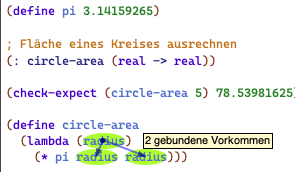
\includegraphics[width=0.5\textwidth]{higher-order/binding}
  \caption{Anzeige von Bindung nach Syntaxprüfung}
  \label{fig:binding}
\end{figure}

Die Beziehung zwischen den Bindung und gebundenen Vorkommen kannst
Du in DrRacket visualisieren, indem Du auf den Knopf
\texttt{Syntaxprüfung} (Englisch \texttt{Check Syntax})
drückst
und dann mit dem Mauszeiger über Variablenvorkommen
streichst.  Abbildung~\ref{fig:binding} zeigt exemplarisch, wie das aussieht.

\begin{aufgabeinline}
  Probiere die \texttt{Syntaxprüfung} auf dem Fußball-Code aus und
  untersuche zum Beispiel die Variablen in der Funktion
  \lstinline{home-points}.
\end{aufgabeinline}

Eine dritte Kategorie von Bindung gibt es auch noch, nämlich die
"<eingebauten"> Variablen wie \texttt{string-append} und
\lstinline{+}, die ähnlich global sichtbar sind wie die globalen
Variablen.  Wenn Du über sie nach \texttt{Syntaxprüfung} streichst,
wird \texttt{importiert aus} angezeigt.

Damit könnte man meinen, es sei alles zur Bindung gesagt: Globale und
eingebaute Variablen sind überall sichtbar; eine lokale Variable ist
innerhalb ihres \lstinline{lambda}-Rumpfes beziehungsweise
\lstinline{cond}-Zweiges sichtbar.  Aber was ist mit der folgenden
Funktion?
%
\begin{lstlisting}
(define f
  (lambda (x)
    (define y (+ x 1))
    (lambda (x)
      (+ x y))))
\end{lstlisting}
%
Die ist zugegeben künstlich konstruiert.  Aber wie verhält sie sich?
%
\begin{aufgabeinline}
  Was liefert die Auswertung von \lstinline{((f 1) 2)}?
\end{aufgabeinline}
%
In dieser Funktion gibt es \emph{zwei} Variablen namens \lstinline{x}:
Zwei Bindungen als Parameter und auch zwei gebundende Vorkommen.
Welche gebundenen Vorkommen gehören zu welchen Bindungen?  Hier gilt
die Regel der sogenannten \textit{lexikalischen Bindung}:
%
\begin{definition}[Lexikalische Bindung]\index{lexikalische Bindung}\index{Bindung!lexikalisch}
  Du findest die zu einem gebundenen Vorkommen zugehörige Bindung,
  indem Du von innen nach außen in der Klammerstruktur der Funktion
  suchst: Die erste Bindung als Parameter oder lokale Definition, die
  Du so findest, gehört zu dem gebundenden Vorkommen.

  Wenn Du auf diese Art und Weise keine Bindung findest, halte
  Ausschau nach einer globalen Definition.  Wenn Du keine globale
  Definition findest, muss es sich um eine eingebaute beziehungsweise
  importierte Definition handeln.
\end{definition}
%
Die lexikalische Bindung ordnet einer Bindung ihre gebundenden
Vorkommen zu.  Das bedeutet, dass Du, wenn Du eine Bindung und all
ihre gebundenen Vorkommen unbenennst, das Verhalten des Programms
nicht änderst.  Entsprechend sind also Variablen, die zu
unterschiedlichen Bindungen gehören, unterschiedliche Variablen.  Wenn
Du nach einer Syntaxprüfung über einer Variable das Kontextmenü
("<rechte Maustaste">) aufrufst, gibt es dort einen Punkt
\texttt{umbenennen}, der das Umbenennen automatisiert.

Die Definition von \lstinline{f} kommt Dir vielleicht esoterisch
vor~-- wir haben künstlich unterschiedliche Variablen gleichen Namens angelegt.
Tatsächlich haben wir aber schon oft Programme geschrieben, bei denen
mehrere Variablen gleichen Namens auftauchen, zuletzt zum Beispiel bei
der Funktion \lstinline{home-points}:

\begin{lstlisting}
(: home-points (game -> points))
...
(define home-points
  (lambda (game)
    ...))
\end{lstlisting}
%
Hier gibt es zwei Variablen namens \lstinline{game}: In der
Signaturdeklaration ist das die Signatur \lstinline{game} aus der
gleichnamigen Record-Definition.  In der Funktion ist es der Parameter
\lstinline{game}.  Dieser erfüllt die Signatur \lstinline{game}~--
darum haben die Signatur und der Parameter ja gerade den gleichen
Namen, um diese Beziehung deutlich zu machen.

Der Begriff "<lexikalische Bindung"> suggeriert, dass es noch andere
Formen der Bindung gibt: Tatsächlich funktioniert Bindung in einigen
anderen, vornehmlich älteren Sprachen, nach anderen Prinzipien, oft
unter dem Begriff \textit{dynamische Bindung}\index{dynamische
  Bindung}\index{Bindung!dynamisch} zusammengefasst.  Lexikalische
Bindung wird oft auch \textit{statische Bindung}\index{statische
  Bindung}\index{Bindung!statisch} genannt.  "<Statisch"> bedeutet
im Kontext der Programmierung "<bevor das Programm läuft"> und
statische Bindung bedeutet, dass Du die Beziehung zwischen Bindungen
und gebundenen Vorkommen am Programmtext ablesen kannst.  Bei
dynamischer Bindung ergibt sich diese Beziehung erst, wenn das
Programm läuft.

Man könnte meinen, \emph{jetzt} wäre alles gesagt zur Bindung.  Aber
es gibt noch eine weitere Besonderheit, nämlich wenn in einer
Definition (gleich ob lokal oder global) die Variable, die definiert
wird, auch gleich wieder auftaucht.  Auch davon haben wir schon
ständig Gebrauch gemacht, nämlich in rekursiven Funktionen, wo für den
rekursiven Aufruf genau die Variable benutzt wird, in deren Definition
sie sich befindet.

\begin{aufgabeinline}
  Zu welchen Bindungen gehören die gebundenden Vorkommen von
  \lstinline{x} in folgendem Programm?
\begin{lstlisting}
(define g
  (lambda (x)
    (define x (+ x 1))
    (define y (+ x 1))
    (lambda (x)
      (+ x y))))
\end{lstlisting}
  Kannst Du vorhersagen~-- ohne es in der REPL auszuprobieren~-- was
  \lstinline{((g 1) 2)} liefert?
\end{aufgabeinline}


\section*{Aufgaben}

\begin{aufgabe}
  Schreibe eine Funktion \lstinline{any?}, die eine Liste akzeptiert
  sowie eine Funktion, die für jedes Listenelement entweder
  \lstinline{#t} oder \lstinline{#f} liefert.  \lstinline{Any?} soll
  \lstinline{#t}
  zurückgeben, wenn mindestens die Funktion für mindestens ein Element
  der Liste \lstinline{#t} zurückgibt, sonst \lstinline{#f}.  

  Schreibe eine analoge Funktion
  \lstinline{every?}, die dann \lstinline{#t} zurückgibt, wenn die Funktion
  für alle Elemente der Liste \lstinline{#t} zurückgibt, sonst \lstinline{#f}.
  Schreibe zunächst eine Fassung nach dem Muster von \lstinline{any?}.
  Schreibe eine zweite Fassung, die einfach \lstinline{any?} aufruft
  und selbst keine Rekursion benutzt.
\end{aufgabe}

\begin{aufgabe}
  Schreibe Funktionen \lstinline{feed-animals} und
  \lstinline{run-over-animals} die mit Hilfe der Funktionen in
  Abschnitt~\ref{sec:feed-animal} auf Seite~\pageref{sec:feed-animal}
  alle Tiere einer Liste
  füttert respektive überfährt.
\end{aufgabe}

\begin{aufgabe}
  Schreibe folgende Funktionen unter der  
  Verwendung von \lstinline{filter}!
  \begin{itemize}
    \item Schreibe eine Funktion \lstinline{evens}, welche die ungeraden Zahlen aus 
      einer Liste entfernt,
  \item eine Funktion \lstinline{count-zeroes}, die in einer Liste von
    Zahlen die Nullen zählt,
  \item und eine Funktion \lstinline{multiples}, die eine Zahl $n$ und
    eine Liste von Zahlen akzeptiert, und eine Liste alle Vielfachen
    der Zahl $n$ liefert.
  \end{itemize}
\end{aufgabe}

\begin{aufgabe}
  Programmiere eine Funktion
  \lstinline{filter-map}, die als Argumente eine Funktion \lstinline{p} mit
  einem Argument sowie eine Liste \lstinline{l} akzeptiert.
  \lstinline{Filter-map} soll als Ergebnis die Liste der Rückgabewerte
  von \lstinline{p} für diejenigen Elemente von \lstinline{l} zurückgeben,
  für die \lstinline{p} nicht \lstinline{#f} zurückgibt.

  Beispiel:

\begin{lstlisting}
(filter-map (lambda (x)
               (if (even? x)
                  (+ x 1)
                  #f))
            (list 1 2 5 17 24 13))
|\evalsto| #<list 3 25>
\end{lstlisting}
\end{aufgabe}

\begin{aufgabe}
  Verwende die Funktion \lstinline{list-fold} um folgende 
  Funktionen zu schreiben:
  \begin{enumerate}
  \item Schreibe eine neue Version der Funktion \lstinline{list-map},
    die eine Funktion auf jedes Element einer Liste anwendet und die
    Liste der Ergebnisse liefert.
  \item Schreibe eine Funktion \lstinline{list-or}, die eine Funktion
    auf alle Elemente einer Liste anwendet, die jeweils ein Boolean
    liefert, und die Resultate mit \lstinline{or} verknüpft.
  \item Schreibe eine Funktion \lstinline{count-trues}, die ein
    Funktion mit boolescher Rückgabe auf
    alle Elemente einer Liste anwendet und zählt, wie häufig \lstinline{#t}
    zurückgegeben wird.
  \item Schreibe eine Funktion \lstinline{contains?}, die
    \lstinline{#t} liefert, wenn ein
    Element in einer Liste enthalten ist, sonst \lstinline{#f}.
  \item Schreibe eine Funktion \lstinline{remove-duplicates}, die alle doppelten
    Elemente aus einer Liste filtert.
  \end{enumerate}
\end{aufgabe}

\begin{aufgabe}
  Fußballreporter zitieren gern obskure Fakten über
  vergangene Spiele, wenn sie zum Spielverlauf wenig zu sagen haben.

  Hier ein Beispiel:
  % 
  \begin{quote}
    "<In der Saison 2009/2010 gab es ja immerhin vier Spieltage, an
    denen die größte Tordifferenz kleiner als 3 war.">
  \end{quote}
  %
\begin{enumerate}
\item Stelle dem Fußballreporter Hilfsfunktionen zur Verfügung,
  die ihm erlauben, eine Antwort auf solch eine Frage zu
  finden:
  %
  \begin{quote}
    \emph{An wie vielen Spieltagen der Saison 2009/2010 war die größte
    Tordifferenz kleiner als 3?}
  \end{quote}
  %
  Schreibe mit Hilfe dieser Funktionen einen Ausdruck, der
  testet, ob die am Anfang dieser Aufgabe zitierte Aussage über die
  Tordifferenzen in der Saison 2009/2010 stimmt!

  \begin{enumerate}
  \item Schreibe eine Funktion, die aus einer Liste die Dubletten
    entfernt.  Diese Funktion akzeptiert eine Liste sowie eine
    Funktion, die zwei Elemente der Liste akzeptiert und
    zurückliefert, ob diese gleich sind.  (Also zum Beispiel
    \lstinline{=} bei Listen von Zahlen.)  Sie liefert dann eine Liste,
    in der jedes Element "<nur einmal vorkommt">, also kein anderes,
    das dazu gleich ist.
  \item Schreibe eine Funktion, die aus der Liste aller Spiele
    eine Liste aller Spielplannummern extrahiert.
  \item Schreibe eine Funktion, die aus der Liste aller Spiele
    eine Liste von Listen aller Spiele macht~-- so dass in jeder
    Teilliste alle Spiele eines Spieltags zusammengefasst sind.
  \item Schreibe eine Funktion, welche die Tordifferenz eines
    Spiels zurückliefert.
  \item Schreibe eine Funktion, welche das maximale Element einer
    Liste berechnet.  Die Funktion sollte neben der Liste eine
    Funktion akzeptieren, die berechnet, ob ein Element "<kleiner oder
    gleich"> einem anderen ist.
  \item Schreibe schließlich einen Ausdruck, der die Anzahl der
    Spieltage der Saison 2009/2010 liefert, bei denen die größte
    Tordifferenz kleiner als 3 war.
  \end{enumerate}

  \item Schreibe Ausdrücke, die folgende Fragen beantworten~--
  entwickele dazu, falls nötig, weitere Hilfsfunktionen:
  \begin{itemize}
    \item An welchem Spieltag gab es die meisten Heimsiege?
    \item An welchem Spieltag fielen die meisten Tore?
    \item Gab es mehr Siege für die Heimmanschaften an ungeraden Spieltagen als an
      geraden?
    \end{itemize}
\end{enumerate} 

\end{aufgabe}

\begin{aufgabe}

  Betrachte das folgende Programm:

\begin{lstlisting}
(define x 2)          ;  --> zwei
(define y -1)         ;  --> minuseins
(define z -3)         ;  --> minusdrei
(define f 
  (lambda (x z)
    (+ (* x x) z y)))
(f 4 -2)
\end{lstlisting}
  %
  Benenne die Variablen \lstinline{x}, \lstinline{y} und \lstinline{z}, die in
  den ersten drei Zeilen des Programms definiert werden, im kompletten
  Programm um, und zwar \lstinline{x} in \lstinline{zwei}, \lstinline{y} in
  \lstinline{minuseins} und \lstinline{z} in \lstinline{minusdrei}. Achte bei
  der Umbenennung auf die lexikalische Bindung.  Benenne keine
  Parameter der Funktion \lstinline{f} um.

  Nachdem Du die Umbenennung durchgeführt hast, welches Ergebnis liefert
  der Ausdruck \lstinline{(f 4 -2)}?
\end{aufgabe}

\begin{aufgabe}

  Betrachte das folgende Programm:

\begin{lstlisting}
(define x 2)                    ; --> zwei
(define y 4)                    ; --> vier
(define z                       ; --> f
  (lambda (x y z)
    (+ x (z y))))

(z y x (lambda (z) (+ x z)))
\end{lstlisting}
%
  Benenne die Variablen \lstinline{x}, \lstinline{y} und \lstinline{z}, die in
  den ersten drei Zeilen des Programms definiert werden, im kompletten
  Programm um. Der neue Name der Variable steht als Kommentar im
  Programm hinter dem Pfeil (\lstinline{-->}).  Achte bei der
  Umbenennung auf die lexikalische Bindung.  Benenne keine
  Parameter der Funktion \lstinline{z} um.

  Berechne, nachdem Du die Umbenennung durchgeführt haben, von
  Hand \lstinline{(z y x}
  \lstinline{(lambda (z) (+ x z))))} und halte die Zwischenschritte
  fest.

\end{aufgabe}

\begin{aufgabe}
  Betrachte folgendes Programm:

\begin{lstlisting}
(define x 1)
(define y 3)
(define z 5)
(define f
  (lambda (x)   
     ((lambda (y)
        ((lambda (z)
           (+ z (* x y)))
         (+ x z)))
      (+ x y))))
(f y)
\end{lstlisting}

  Benenne hier alle lokalen Variablen, die innerhalb der Funktion
  \lstinline{f} gebunden werden, um. Verändere nicht den Namen der
  Variablen \lstinline{x}, \lstinline{y} und \lstinline{z} aus den ersten drei Zeilen
  des Programms.  Welches Ergebnis liefert
  der Ausdruck \lstinline{(f y)} nach der Umbenennung?
\end{aufgabe}

\begin{aufgabe}
  Programmiere ein einfaches Telefonbuch: Ein Telefonbuch ist
  als Funktion repräsentiert, die den Namen einer Person akzeptiert
  und die Telefonnummer der Person zurückliefert.

  \begin{enumerate}
  \item Definiere zunächst eine Signatur
    \lstinline{phonebook-result} für das Ergebnis des Nachschlagens in einem
    Telefonbuch. Ein solches Ergebnis ist entweder eine Telefonnummer
    oder ein Wert, der "<nicht gefunden"> darstellt,

    Die Signatur des Telefonbuchs ist  \lstinline{(string -> phonebook-result)}.
  \item Definiere einen Wert \lstinline{empty-phonebook}, der das leere
    Telefonbuch repräsentiert.
  \item Definiere eine Funktion 
    \lstinline{add-to-phonebook}, die ein Telefonbuch, einen Namen
    und eine Telefonnummer erwartet und das um den neuen Eintrag
    erweiterte
    Telefonbuch zurückliefert.
  \item Schreibe eine Funktion \lstinline{lookup-in-phonebook},
    die ein Telefonbuch und einen Namen einer Person erwartet und die
    Nummer der Person im Telefonbuch zurückliefert.
    Beispiele:
    \begin{itemize}
    \item \lstinline{(lookup-in-phonebook empty-phonebook "Hans")} liefert
      "<nicht gefunden">.
    \item \lstinline{(lookup-in-phonebook} \\
      \lstinline{    (add-to-phonebook empty-phonebook "Hans" "754829")}\\
      \lstinline{    "Hans")} \\
      liefert die Nummer 754829.
    \item \lstinline{(lookup-in-phonebook}\\
      \lstinline{    (add-to-phonebook empty-phonebook "Hans" "754829")}\\
      \lstinline{    "Lea")}\\
      liefert "<nicht gefunden">.
    \end{itemize}
  \end{enumerate}
\end{aufgabe}

\begin{aufgabe}
  Diese Aufgabe ist für Dich geeignet, falls Du das entsprechende
  Wissen aus der Mathematik besitzt:

  Ein Polynom ist eine Funktion von $\mathbb{R}$ nach $\mathbb{R}$ und
  hat folgende Form:
  \begin{displaymath}
    p(x) = a_0 +
    a_1 \times x + a_2 \times x^2 + \ldots + a_n \times x^n    
  \end{displaymath}
  %
  Ein Polynom wird also eindeutig durch die Koeffizienten $a_0$ bis
  $a_n$ bestimmt.

  \begin{enumerate}
   \item Schreibe die Datendefinition für Polynome.
   \item Programmiere eine Funktion \lstinline{polynomial+}, die
     zwei Polynome addiert.  Schreibe ggf.\ zutreffende Eigenschaften auf
     und überprüfe diese!
     
   \item Programmiere eine Funktion \lstinline{polynomial*}, die zwei Polynome 
     multipliziert. 
     Beispielsweise werden die Polynome $a_0+a_1 x$ und $b_0+b_1 x$ nach folgendem Schema multipliziert:
     \begin{eqnarray*}
     & &a_0 \times (b_0+b_1\times x) \\
     &+&a_1 x \times (b_0+b_1\times x) \\ 
     &=&a_0\times b_0+a_0\times b_1 x + a_1\times b_0x + a_1\times b_1x^2
     \end{eqnarray*}	
     Schreibe ggf.\ zutreffende Eigenschaften auf und überprüfe diese!
   \item Schreibe eine Funktion \lstinline{polynomial-function}, die
     ein Polynom akzeptiert und eine Funktion liefert, die ein Polynom
     an einer bestimmten Stelle auswertet, also gerade der Funktion
     $p$ aus der Definition entspricht. 
   \item Die Ableitung eines Polynoms $p$ wie oben ist bekanntlich durch
     \begin{displaymath}
       p'(x) = a_1 + 2\times a_2 \times x + 3\times a_3\times x^2 + \ldots
       + n \times a_n \times x^{n-1}
     \end{displaymath}
     gegeben. Schreibe die Funktion
     \lstinline{polynomial-derivative}, die von einem gegebenen Polynom das abgeleitete Polynom
     berechnet.
 \end{enumerate}
\end{aufgabe}

\begin{aufgabe}
  Listen lassen sich nach verschiedenen Kriterien
  sortieren: zum Beispiel aufsteigend, absteigend, oder abhängig von
  einem Feld der Elemente.  So kann eine Liste von Fußballspielen nach
  der Gesamtanzahl der Tore, der Anzahl der Tore des Heimteams oder
  der Anzahl der Tore des Gästeteams oder der Anzahl der Tore der
  gewinnenden Mannschaft sortiert werden.  Das Kriterium für die
  Sortierung wird durch
  eine Funktion festgelegt, die ermittelt, ob ein Elemente vor einem anderen
  stehen soll.

\begin{enumerate}
\item Schreibe eine Funktion, die eine Liste nach einem beliebigen
  Kriterium sortiert.  Die Funktion sollte folgende Signatur haben:

\begin{lstlisting}
(: list-sort ((%a %a -> boolean) (list-of %a) -> (list-of %a)))
\end{lstlisting}

  Das erste Argument ist eine Funktion, die eine \textit{Ordnung}
  realisiert, also zwei Elemente vergleicht, und \lstinline{#t}
  zurückliefert, falls sie schon in der richtigen Reihenfolge sind und
  \lstinline{#f}, falls nicht.  Zum Beispiel können \lstinline{<=} oder \lstinline{>=}
  für das Sortieren von Listen von Zahlen verwendet werden.
\item Benutze diese Funktion, um eine Liste von
  Fußballspielen nach den folgenden Kriterien zu sortieren:
  \begin{itemize}
  \item Gesamtanzahl der Tore,
  \item Anzahl der Tore der Heimmannschaft,
  \item Anzahl der Tore des Gastmannschaft oder
  \item Anzahl der Tore der
    gewinnenden Mannschaft
  \end{itemize}
\end{enumerate}
\end{aufgabe}

\begin{aufgabe}
  Folgen mit unendlicher Länge lassen sich als
  zusammengesetzte Daten mit zwei Komponenten repräsentieren: Dabei
  ist die erste Komponente das erste Element der Folge und die zweite
  eine Funktion ohne Parameter, die, wenn sie angewendet wird, eine Folge mit
  den restlichen Elementen ohne das erste liefert.
  Solche unendlichen Folgen heißen \textit{Streams}.
  Schreibe Daten- und Record-Definition für Streams!

  Folgende Funktion soll einen Stream aus natürlichen Zahlen liefern,
  ab einer Zahl $n$:
  % 
  \indexvariable{from}
\begin{lstlisting}
; Stream mit Zahlen ab n erzeugen
(: from (natural -> stream))
(define from
  (lambda (n)
    (make-stream n
                 (lambda () (from (+ n 1))))))
  \end{lstlisting}
  % 
  (Dabei ist angenommen, dass der Konstruktor der Record-Definition
  \lstinline{make-stream} heißt.)
  Zur Betrachtung von Streams ist folgende Funktion nützlich, welche
  die ersten $n$ Elemente eines Streams als Liste extrahiert:
  % 
  \indexvariable{stream-take}
\begin{lstlisting}
; erste Elemente eines Streams in eine Liste extrahieren
(: stream-take (natural stream -> (list-of %a)))
(define stream-take
  (lambda (n stream)
    (if (= n 0)
        empty
        (cons (stream-first stream)
              (stream-take (- n 1)
                           ((stream-rest-function stream)))))))
\end{lstlisting}
   % 
   (Dabei haben wir angenommen, dass die Selektoren
   \lstinline{stream-first} und \lstinline{stream-rest-function} heißen.)

   \lstinline{Stream-take} lässt sich zum Beispiel auf das Ergebnis von
   \lstinline{from} anwenden:
   % 
\begin{lstlisting}
(stream-take 17 (from 4))
|\evalsto| #<list 4 5 6 7 8 9 10 11 12 13 14 15 16 17 18 19 20>
\end{lstlisting}
   % 
   Programmiere einige intellektuelle Herausforderungen mit Streams!
   \begin{enumerate}
   \item Programmiere eine Funktion \lstinline{stream-drop}, die eine
     natürliche Zahl $n$ und einen Stream akzeptiert, und einen neuen
     Stream liefert, der aus dem alten durch Weglassen der ersten $n$
     Elemente entsteht:
\begin{lstlisting}
(stream-take 17 (stream-drop 3 (from 4)))
|\evalsto| #<list 7 8 9 10 11 12 13 14 15 16 17 18 19 20 21 22 23>
\end{lstlisting}
   \item Programmiere eine Funktion \lstinline{stream-filter} analog zu
     \lstinline{filter}:
     % 
\begin{lstlisting}
(stream-take 10 (stream-filter odd? (from 1)))
|\evalsto| #<list 1 3 5 7 9 11 13 15 17 19>
\end{lstlisting}
   \item Programmiere eine Funktion \lstinline{drop-multiples}, die 
     eine Zahl $n$ und einen Stream von Zahlen $s$ akzeptiert.
     \lstinline{Drop-multiples} soll einen Stream liefern, in dem
     gegenüber $s$  alle Vielfachen von $n$ entfernt wurden:
     % 
\begin{lstlisting}
(stream-take 10 (drop-multiples 3 (from 1)))
|\evalsto| #<list 1 2 4 5 7 8 10 11 13 14>
\end{lstlisting}
   \item Schreibe eine Funktion \lstinline{sieve}, die aus einem Stream
     von Zahlen all diejenigen Zahlen entfernt, die Vielfache von
     Vorgängern im Stream sind:
\begin{lstlisting}
(stream-take 10 (sieve (from 2)))
|\evalsto| #<list 2 3 5 7 11 13 17 19 23 29>
\end{lstlisting}
     Um was für Zahlen handelt es sich in dem Beispielaufruf und
     warum?
   \item Schreibe eine Funktion \lstinline{powers}, die für eine Zahl
     $n$ einen Stream ihrer Potenzen liefert:
     % 
\begin{lstlisting}
(stream-take 10 (powers 2))
|\evalsto| #<list 2 4 8 16 32 64 128 256 512 1024>
\end{lstlisting}
   \item Schreibe eine Funktion \lstinline{stream-map} analog zu
     \lstinline{list-map}:
\begin{lstlisting}
(stream-take 10 (stream-map (lambda (x) (+ x 1)) (from 1)))
|\evalsto| #<list 2 3 4 5 6 7 8 9 10 11>
\end{lstlisting}
   \item Schreibe eine Funktion \lstinline{merge}, die zwei
     aufsteigende Streams von Zahlen zu einem aufsteigenden Stream
     der Elemente beider Streams vereinigt:
\begin{lstlisting}
(stream-take 10 (merge (powers 2) (powers 3)))
|\evalsto| #<list 2 3 4 8 9 16 27 32 64 81>
\end{lstlisting}
   \item Schreibe eine Definition für einen Stream aufsteigend
     sortierter Potenzen von Primzahlen:
\begin{lstlisting}
(stream-take 10 prime-powers)
|\evalsto| #<list 2 3 4 5 7 8 9 11 13 16>
\end{lstlisting}
     Definiere dazu zunächst einen Stream aus Streams von Potenzen
     % 
     \indexvariable{prime-powers-stream}
\begin{lstlisting}
(define prime-powers-stream (stream-map powers (sieve (from 2))))
\end{lstlisting}
     % 
     Definiere eine Funktion \lstinline{merge-streams}, welche
     diesen Stream akzeptiert und die Elemente der Streams
     aus \lstinline{prime-powers-stream} mit Hilfe von \lstinline{merge}
     aufsteigend sortiert.
   \end{enumerate}
 \end{aufgabe}

 \begin{aufgabe}
  Betrachte folgende mysteriöse Funktion:
\begin{lstlisting}
(: // ((%a -> (%b -> %b)) (list-of %a) -> (%b -> %b)))

(define //
  (lambda (proc lis)
    (cond
      ((empty? lis)
       (lambda (y)
         y))
      ((cons? lis)
       (lambda (y)
         ((proc (first lis))
          ((// proc (rest lis))
           y)))))))
\end{lstlisting}
  % 
  \textbf{Hinweise:} Beachte die Signaturen! In mehreren
  Teilaufgaben gibt es Gelegenheiten, \lstinline{curry} beziehungsweise
  \lstinline{uncurry} zu benutzen.

  \begin{itemize}
  \item Vergleiche die Funktion mit \lstinline{list-fold} und
    beschreibe, wie \lstinline{//} und \lstinline{list-fold} zueinander
    in Beziehung stehen.  Schreibe, falls möglich, eine
    Definition von \lstinline{//}, die \lstinline{list-fold} benutzt und
    umgekehrt.
  \item Schreibe mit Hilfe von \lstinline{//} eine Funktion
    \lstinline{list-sum}, welche die Elemente einer Liste addiert.
  \item Schreibe eine Funktion \lstinline{insert}, die eine reelle
    Zahl $n$ akzeptiert und eine Funktion zurückliefert, die eine
    aufsteigend sortierte Liste von reellen Zahlen konsumiert und
    eine Liste zurückliefert, in der $n$ an die entsprechende
    Stelle der Liste einsortiert wurde.
  \item Schreibe mit Hilfe von \lstinline{//} eine Funktion, die
    eine Liste von reellen Zahlen aufsteigend sortiert.
  \end{itemize}
\end{aufgabe}


\begin{aufgabe}
  Betrachte folgendes mysteriöse Programm:
  % 
  \begin{lstlisting}
(define y
  (lambda (f)
    ((lambda (x)
       (f (lambda (z) ((x x) z))))
     (lambda (x)
       (f (lambda (z) ((x x) z)))))))

(define m
  (y
   (lambda (f)
     (lambda (x)
       (cond
         ((= x 1)
          1)
         ((> x 1)
          (* x (f (- x 1)))))))))
   \end{lstlisting}
  %
  Probiere \lstinline{m} aus~-- was macht die Funktion?

  Die Funktion \lstinline{y}
  wird auch \textit{Fixpunktkombinator}\index{Fixpunktkombinator}
  genannt.  Das Thema kommt in Abschnitt~\ref{sec:fixpunktsatz} auf
  Seite~\pageref{sec:fixpunktsatz} noch einmal ausführlich:
 \end{aufgabe}

\begin{aufgabe}
  Beweise, dass für Funktionen $p_1$ mit einem Parameter, die
  einparametrige Funktionen zurückgeben, und Funktionen $p_2$ mit zwei
  Parametern gilt:
  %
  \begin{center}
    \lstinline{(curry (uncurry $p_1$))} $=$ $p_1$\\
    \lstinline{(uncurry (curry $p_2$))} $=$ $p_2$
  \end{center}
 \end{aufgabe}

\begin{aufgabe}
  Eine Funktion $f$ ist \textit{idempotent}\index{idempotent}, wenn gilt:

  \begin{center}
    \lstinline{(compose $f$ $f$) $=$ $f$}
  \end{center}

  Zeige, dass folgende Funktion idempotent ist:

  \indexvariable{abs}
  \begin{lstlisting}
    (define abs
      (lambda (x)
         (if (negative? x)
             (- x)
             x)))  \end{lstlisting}

  Welche anderen idempotente Funktionen kennst Du?
\end{aufgabe}

%%% Local Variables: 
%%% mode: latex
%%% TeX-master: "i1"
%%% End: 


% Diese Datei ist Teil des Buchs "Schreibe Dein Programm!"
% Das Buch ist lizensiert unter der Creative-Commons-Lizenz
% "Namensnennung - Weitergabe unter gleichen Bedingungen 4.0 International (CC BY-SA 4.0)"
% https://creativecommons.org/licenses/by-sa/4.0/deed.de

\chapter{Programmieren mit Akkumulatoren}
\label{cha:accu}

Manche Berechnungen funktionieren am einfachsten, wenn sie ein
Zwischenergebnis mitführen und aktualisieren.  Die bisherigen
Konstruktionsanleitungen für Funktionen, die Listen oder natürliche
Zahlen verarbeiten, können das aber nicht.  Wir brauchen dafür eine
neue Programmiertechnik, das Programmieren mit
\textit{Akkumulatoren}, und entsprechend angepasste
Konstruktionsanleitungen.  Beides behandeln wir in diesem Kapitel.

\section{Zwischenergebnisse mitführen}
\label{sec:intermediate-results}

\mentioncode{akkumulatoren/accumulator.rkt}
%
Wir fangen mit einer scheinbar einfachen Funktion an: Gefragt ist eine
Funktion, die eine Liste invertiert, also die Reihenfolge ihrer
Elemente umdreht:\indexvariable{invert}\label{sec:invert}
%
\begin{lstlisting}
; Liste umdrehen
(: invert ((list-of %a) -> (list-of %a)))

(check-expect (invert empty) empty)
(check-expect (invert (list 1 2 3 4)) (list 4 3 2 1))
\end{lstlisting}
%
Gerüst und Schablone sehen wie folgt aus:
%
\begin{lstlisting}
(define invert
  (lambda (list)
    (cond
      ((empty? list) ...)
      ((cons? list)
      ... (invert (rest list)) ...
      ... (first list) ...))))
\end{lstlisting}
%
Um den Rumpf zu vervollständigen, können wir uns an dem zweiten
Testfall orientieren~-- da ist \lstinline{list} die Liste mit den
Elementen 1 2 3 4.  Entsprechend ist \lstinline{(first list)} die
Zahl 1, \lstinline{(rest list)} die Liste mit den Elementen 2 3 4, das
heiß der rekursive Aufruf liefert die Liste mit den Elementen 4 3 2.
Um das gewünschte Ergebnis mit den Elementen 4 3 2 1 zu bekommen,
müssen wir deshalb \lstinline{(first list)} hinten an das Ergebnis des
rekursiven Aufrufs anhängen.

Um ein Element \emph{hinten} an eine Liste zu hängen, haben wir bisher
noch keine fertige Funktion~-- die müssen wir erst noch schreiben.
Wir könnten die Arbeit jetzt unterbrechen, um das zu tun.  Wir machen
erstmal nur eine Notiz, dass wir das später machen~-- in Form einer
Kurzbeschreibung und einer Signatur:
%
\begin{lstlisting}
; Element an Liste anhängen
(: append-element ((list-of %a) %a -> (list-of %a)))
\end{lstlisting}
%
Wenn wir diese Funktion voraussetzen, können wir \lstinline{invert}
recht einfach fertigschreiben:
%
\indexvariable{invert}
\begin{lstlisting}
(define invert
  (lambda (list)
    (cond
      ((empty? list) empty)
      ((cons? list)
       (append-element (invert (rest list))
                       (first list))))))
\end{lstlisting}
%
Die Funktion \lstinline{append-element} ist ganz ähnlich der Funktion
\lstinline{concatenate} aus Abschnitt~\ref{sec:more-lists}.  Zunächst
Testfälle:
%
\begin{lstlisting}
(check-expect (append-element (list 1 2 3) 4) (list 1 2 3 4))
(check-expect (append-element empty 4) (list 4))
\end{lstlisting}
%
Gerüst und Schablone:
%
\begin{lstlisting}
(define append-element
  (lambda (list element)
    (cond
      ((empty? list) ...)
      ((cons? list)
       ... (first list) ...
       ... (append-element (rest list) element) ...))))
\end{lstlisting}
%
Im \lstinline{cons}-Fall können wir auch hier die Lösung anhand eines
Beispiels finden: Im Testfall hat \lstinline{list} die Elemente 1 2 3,
der rekursive Aufruf liefert also 2 3 4.  Wir müssen
\lstinline{(first list)}, also die 1, nur noch vorne dranhängen, mit
\lstinline{cons}. Im \lstinline{empty}-Fall hängen wir
\lstinline{element} hinten an eine leere Liste~-- wir brauchen deshalb
eine einelementige Liste mit \lstinline{element} drin, das könnten wir
mit der eingebauten \lstinline{list} machen:
%
\begin{lstlisting}
(define append-element
  (lambda (list element)
    (cond
      ((empty? list) (list element))
      ((cons? list)
       (cons (first list)
             (append-element (rest list) element))))))
\end{lstlisting}
%
Hier wollten wir gern "<Fertig!"> wie sonst auch schreiben, aber die
Funktion funktioniert nicht: DrRacket beschwert sich, dass nach der
öffnenden Klammer von \lstinline{(list element)} keine Funktion steht
sondern \lstinline{#<empty-list>}.  Wups!  Das liegt daran, dass wir
zwar in \lstinline{(list element)} die eingebaute Funktion
\lstinline{list} gemeint haben,
wir aber auch einen Parameter mit dem Namen \lstinline{list}
benutzen, und der
überdeckt nach den Regeln der lexikalischen Bindung aus
Abschnitt~\ref{sec:lexikalische-bindung} auf
Seite~\pageref{sec:lexikalische-bindung} die
eingebaute Funktion.

Wir können das Problem auf zwei Arten lösen~-- wir benennen den
Parameter um oder wir konstruieren die einelementige Liste "<von
Hand">.  Wir haben uns für letzteres entschieden:
%
\indexvariable{append-element}
\begin{lstlisting}
(define append-element
  (lambda (list element)
    (cond
      ((empty? list) (cons element empty))
      ((cons? list)
       (cons (first list)
             (append-element (rest list) element))))))
\end{lstlisting}

Doch zurück zu \lstinline{invert}.  Obwohl die zu erledigende Aufgabe
einfach erscheint, dauert schon das Invertieren von Listen der Länge
1000 eine ganze Weile.  Du kannst das zum Beispiel ausprobieren, indem
Du die Funktion \lstinline{copies} aus Abschnitt~\ref{func:copies} auf
Seite~\pageref{func:copies} verwendest und das hier in der REPL auswertest:
%
\begin{lstlisting}
(invert (copies 1000 42))
\end{lstlisting}
%
Das dauert 2020 auf dem kaum ein Jahr alten Computer von Michael
Sperber immerhin ein
paar Sekunden: Das wäre vielleicht in den 70er Jahren noch akzeptabel
gewesen.  Tatsächlich ist es so, dass zum Beispiel
das Invertieren einer Liste der Länge 400 \emph{mehr} als doppelt so
lang wie das Invertieren einer Liste der Länge 200 benötigt.  Das
liegt daran, dass \lstinline{invert} bei jedem rekursiven Aufruf
\lstinline{append-element} aufruft, und \lstinline{append-element} selbst
macht soviele rekursive Aufrufe wie die Liste lang ist. Das sind für
eine Liste der Länge 20 für den ersten Aufruf von
\lstinline{append-element} 19 Aufrufe, für den zweiten 18 Aufrufe
undsoweiter.

Das sind also $19+18+17+\ldots+1$ rekursive Aufrufe.  Vielleicht
erinnerst Du Dich~-- das ist ein Beispiel für die Gaußsche
Summenformel, die wir in Abschnitt~\ref{sec:gausssche-summenformel}
auf Seite~\pageref{sec:gausssche-summenformel} bewiesen haben:
%
\[\forall n\in\mathbb{N}: \sum_{i=0}^n i =
  \frac{n\times (n+1)}{2}\]
%
\begin{figure}[tb]
  \centering
\begin{tikzpicture}
  \begin{axis}[
    title={Anzahl der rekursiven Aufrufe},
    xlabel={Anzahl $n$ der Listenelemente},
    ylabel={$\frac{n\times (n+1)}{2}$}
    ]
    \addplot [
    blue,
    domain=0:10,
    samples=10,
    ]
    {x*(x+1)/2};
  \end{axis}
\end{tikzpicture}
  \caption{Funktionaufrufe bei \lstinline{invert}}
  \label{fig:invert-calls}
\end{figure}

\noindent Wenn Du diese Formel für immer größer werdende $n$ ausrechnest, wird
die Zahl schwindelerregend schnell größer, wie
Abbildung~\ref{fig:invert-calls} zeigt.  Woran liegt das?

Wenn Du die rechte Seite ausmultiplizierst, steht da:
\[ \frac{n\times (n+1)}{2} = \frac{n^2 + n}{2} \]
%
In der Formel bestimmt das $n^2$ das schnelle Wachstum, auch
\textit{quadratisch} genannt.\index{quadratisches Wachstum}

Tatsächlich gibt es eine bessere Methode, eine Liste umzudrehen: Die
obige \lstinline{invert}"=Funktion konstruiert die Ergebnisliste, indem
stets Elemente \emph{hinten} angehängt werden.  Das entspricht 
nicht der "<natürlichen"> Konstruktion von Listen mit
\lstinline{cons}, das ein Element \emph{vorn} anhängt.  
Das Ergebnis ließe sich aber durch Anhängen vorn ganz einfach
konstruieren, und zwar, indem in folgender Reihenfolge
Zwischenergebnisse\index{Zwischenergebnis} berechnet werden, wie in folgendem Beispiel für den
Testfall \lstinline{(invert (list 1 2 3 4))}:
%
\begin{lstlisting}
#<empty-list>
#<list 1>
#<list 2 1>
#<list 3 2 1>
#<list 4 3 2 1>
\end{lstlisting}
%
Jedes Zwischenergebnis entsteht aus dem vorhergehenden, indem ein
Element vorn an die Liste darüber angehängt wird.  Dies geschieht in
der Reihenfolge, in der die Elemente in der ursprünglichen Liste
auftreten: scheinbar einfach.  Allerdings erlaubt die normale
Konstruktionsanleitung für Listen nicht, dieses Zwischenergebnis
mitzuführen: Das Ergebnis des rekursiven Aufrufs
\lstinline{(invert (rest lis))} ist unabhängig vom Wert von
\lstinline{(first lis)}.  Damit aber
ist es der Funktion aus der normalen Konstruktionsanleitung unmöglich,
die obige Folge von Zwischenergebnissen nachzuvollziehen, da von einem
Zwischenergebnis zum nächsten gerade \lstinline{(first lis)} vorn
angehängt wird.  Wir müssen also etwas anders an das Problem herangehen.

Um das Zwischenergebnis mitzuführen, 
benutzen wir einen separaten Parameter, einen sogenannten
\textit{Akkumulator\index{Akkumulator}}.  Dieser sammelt die
invertierte Liste der bisher schon "<gesehenen"> Elemente auf.  Hier
ist die Signatur der neuen Funktion \lstinline{invert-helper}:
%
\begin{lstlisting}
; Hilfsfunktion zum Umdrehen einer Liste
(: invert-helper ((list-of %a) (list-of %a) -> (list-of %a)))
\end{lstlisting}
%
Der folgende Testfall soll illustrieren, wie die Funktion arbeitet:
\begin{lstlisting}
(check-expect (invert-helper (list 4 5 6) (list 3 2 1))
              (list 6 5 4 3 2 1))
\end{lstlisting}
%
Die zweite Liste~-- der Akkumulator~-- enthält die "<bereits
invertierten"> Elemente.  Die erste Liste ist noch nicht verarbeitet;
die Elemente werden nacheinander an den Akkumulator vorn drangehängt.
Für die Definition der Funktion setzen wir erst einmal die bereits
bekannte Schablone ein für Funktionen, die eine Liste akzeptieren:
%
\begin{lstlisting}
(define invert-helper
  (lambda (list inverted)
    (cond
      ((empty? list) ...)
      ((cons? list)
       ... (first list) ...
       ... (invert-helper (rest list) ...) ...))))
\end{lstlisting}
%
Ziemlich viele Lücken noch!  Füllen wir erstmal die einfachste, im
\lstinline{empty}-Fall: Dann nämlich hat die Funktion schon "<alle
Elemente gesehen"> und diese in den Akkumulator \lstinline{inverted}
"<hineinakkumuliert">~-- der enthält dann die invertierte
Eingabeliste:
%
\begin{lstlisting}
(define invert-helper
  (lambda (list inverted)
    (cond
      ((empty? list) inverted)
      ((cons? list)
       ... (first list) ...
       ... (invert-helper (rest list) ...) ...))))
\end{lstlisting}
%
Im \lstinline{cons}-Fall müssen wir insbesondere das Argument zum zweiten
Parameter von \lstinline{invert-helper} ergänzen: Wir sind natürlich
versucht, da einfach \lstinline{inverted} hinzuschreiben wie bei
vielen anderen rekursiven Funktionen vorher.  Aber wir müssen doch die
Elemente von \lstinline{list} da noch "<hineinakkumulieren"> und aus
dem vorigen Zwischenergebnis das nächste machen.  Für das
"<Hineinakkumulieren"> nehmen wir das erste Element und hängen es
vorn an, so wie wir es in der Beispielrechnung auch gemacht haben:
%
\begin{lstlisting}
(define invert-helper
  (lambda (list inverted)
    (cond
      ((empty? list) inverted)
      ((cons? list)
       ...
       (invert-helper (rest list)
                      (cons (first list) inverted))
       ...))))
\end{lstlisting}
%
Was müssen wir noch dazuschreiben?  Die Funktion arbeitet schon die
Eingabeliste ab und akkumuliert ihre Elemente in \lstinline{inverted}
hinein. Sie ist bereits fertig, wir müssen nur die Ellipsen wegmachen:\label{function:invert-helper}
%
\indexvariable{invert-helper}
\begin{lstlisting}
(define invert-helper
  (lambda (list inverted)
    (cond
      ((empty? list) inverted)
      ((cons? list)
       (invert-helper (rest list)
                      (cons (first list) inverted))))))
\end{lstlisting}
%
Die Funktion kann schon was, ist aber natürlich nicht identisch zur
ursprünglichen \lstinline{invert}-Funktion, die ja nur eine Eingabe
hat.  Um "<einfach nur eine Liste umzudrehen">, können wir
\lstinline{invert-helper} mit einem leeren Akkumulator aufrufen, wie
in diesem Testfall:
%
\begin{lstlisting}
(check-expect (invert-helper (list 1 2 3) empty)
              (list 3 2 1))
\end{lstlisting}
%
\begin{aufgabeinline}
  Definiere \lstinline{invert} um, so dass es
  \lstinline{invert-helper} benutzt!
\end{aufgabeinline}
%
Die neue Version von \lstinline{invert} funktioniert nicht nur
korrekt, sondern auch schnell: Sie benutzt keine Hilfsfunktion und
macht soviele rekursive Aufrufe wie die Eingabeliste Elemente hat, ihre
Laufzeit wächst also \textit{linear}.\index{lineares Wachstum}

Übrigens: Da die Funktion \lstinline{invert} generell nützlich ist,
ist sie unter dem Namen
\lstinline{reverse}\indexvariable{reverse} fest eingebaut.

\section{Schablonen für Funktionen mit Akkumulator}

Auch für Funktionen mit Akkumulator entwickeln wir eine
Konstruktionsanleitung.  Vorher wollen wir aber noch einmal
anhand eines weiteren Beispiels Revue passieren lassen, wie der
Konstruktionsprozess bei solchen Funktionen eigentlich genau aussieht.

Wir nehmen uns eine Funktion vor, die wir eigentlich schon kennen,
nämlich aus Abschnitt~\ref{sec:list-sum} auf Seite
\pageref{sec:list-sum}:\label{function:list-sum-acc}
%
\begin{lstlisting}
; Summe der Elemente einer Liste von Zahlen berechnen
(: list-sum ((list-of number) -> number))
\end{lstlisting}
%
Wir nehmen uns allerdings diesmal vor, mit Akkumulator zu arbeiten.
Dazu müssen wir uns erst einmal überlegen, was für Information der
Akkumulator eigentlich akkumulieren soll.  Das sollte ein
\textit{Zwischenergebnis}\index{Zwischenergebnis} sein, das ist 
eine vorläufige Version des gewünschten Endergebnisses.  Da es 
hier das Endergebnis die Summe aller Listenelemente ist, nehmen wir
als Zwischenergebnis die Summer aller Listenelemente, die unsere
Funktion schon "<gesehen"> hat.  Wir nennen deshalb den
Akkumulator \lstinline{sum} und schreiben folgende Schablone:
%
\indexvariable{list-sum-helper}
\begin{lstlisting}
(define list-sum-helper
  (lambda (list sum)
    (cond
      ((empty? list) ... sum ...)
      ((cons? list)
       (list-sum-helper (rest list)
                        (... (first list) ... sum ...))))))
\end{lstlisting}
%
Warum sieht sie gerade so aus, beziehungsweise: Was ist der Unterschied
zur ganz normalen Schablone für Listen als Eingabe aus
Konstruktionsanleitung~\ref{ka:listen-eingabe-schablone} auf
Seite~\pageref{ka:listen-eingabe-schablone}?   Hier ist sie zur
Erinnerung noch einmal:
%
\begin{lstlisting}
(define |\(f\)|
  (lambda (|\ldots| |\(\mathit{list}\)| |\ldots|)
    (cond
      ((empty? |\(\mathit{list}\)|) |\ldots|)
      ((cons? |\(\mathit{list}\)|)
       |\ldots|
       (first |\(\mathit{list}\)|)
       (|\(f\)| (first |\(\mathit{list}\)|))
       |\ldots|
       ))))
\end{lstlisting}
%
Im \lstinline{empty}-Zweig steht der Akkumulator \lstinline{sum},
während in
der Schablone aus
Konstruktionsanleitung~\ref{ka:listen-eingabe-schablone} gar nichts
steht: Hier ist die Liste am Ende und es ist Zeit, das Endergebnis
auszurechnen, das im \lstinline{empty}-Zweig herauskommen soll.   Weil
der Akkumulator ein Zwischenergebnis ist, muss er am Schluss zumindest
nah am
Endergebnis dran sein.  Meist \emph{ist} das letzte
Zwischenergebnis das Endergebnis.

Im \lstinline{cons}-Fall steht ein rekursiver Aufruf mit
\lstinline{(rest list)} als Listen-Argument~-- wie in
Konstruktionsanleitung~\ref{ka:listen-eingabe-schablone} auch.
Außerdem steht dort eine Hilfestellung für die Berechnung des
Akkumulator"=Arguments, also des nächsten Zwischenergebnisses.  Da
sollte das letzte Zwischenergebnis~-- hier \lstinline{sum}~-- und das
nächste Listenelement \lstinline{(first list)} eingehen. Darum stehen
sie in der Schablone.  Dieser Teil der Schablone ist also nur eine
Erweiterung der ursprünglichen Schablone.

Außerdem fällt Dir vielleicht auf, dass um den rekursiven Aufruf herum
keine Ellipsen \lstinline{...} stehen: Du solltest da nichts drumherum
schreiben.  Das liegt daran, dass der letzte rekursive Aufruf von
\lstinline{list-sum-helper} am Ende der Liste das Ergebnis
produziert~-- das muss die Funktion einfach unverändert zurückliefern,
und darum steht da nichts drumherum.

Um die Funktion zu vervollständigen, müssen wir noch klarer als bisher
formulieren, was genau der Akkumulator \lstinline{sum} repräsentiert.
Oben haben wir etwas salopp geschrieben, dass es sich um die Summe
aller Listenelemente handelt, welche die Funktion schon "<gesehen">
hat.  Die sind aber für \lstinline{list-sum-helper} gar nicht mehr
sichtbar.  Wir können sie sichtbar machen, indem wir die Funktion
\lstinline{list-sum} einbeziehen, die \lstinline{list-sum-helper}
aufruft.  Hier ist die Schablone dafür:
%
\begin{lstlisting}
(define list-sum
  (lambda (list0)
    (list-sum-helper list0 ...)))
\end{lstlisting}
%
Wir haben bewusst den Namen \lstinline{list0} gewählt, damit wir ihn
nicht mit dem \lstinline{list} aus \lstinline{list-sum-helper}
durcheinanderbringen.  (Anders als noch bei \lstinline{reverse}~-- wir
versuchen, es besser zu machen.)

\begin{figure}[tb]
  \centering
  \begin{tikzpicture}
    \node (cell1) at (0,0) [draw,thick,minimum width=1cm,minimum height=1cm] {};
    \node (cell2) at (1,0) [draw,thick,minimum width=1cm,minimum height=1cm] {};
    \node (cell3) at (2,0) [draw,thick,minimum width=1cm,minimum height=1cm] {};
    \node (cell4) at (3,0) [draw,thick,minimum width=1cm,minimum height=1cm] {};
    \node (cell5) at (4,0) [draw,thick,minimum width=1cm,minimum height=1cm] {};
    \node (cell6) at (5,0) [draw,thick,minimum width=1cm,minimum height=1cm] {};
    \node (cell7) at (6,0) [draw,thick,minimum width=1cm,minimum height=1cm] {};
    \node (cell8) at (7,0) [draw,thick,minimum width=1cm,minimum height=1cm] {};
    \node (cell9) at (8,0) [draw,thick,minimum width=1cm,minimum height=1cm] {};
    \draw [
    thick,
    decoration={
        brace,
        amplitude=0.3cm,
        mirror,
        raise=0.5cm
    },
    decorate
    ] (cell4.west) -- (cell9.east) 
    node [midway,yshift=-0.9cm] {\lstinline{list}};
    \draw [
    thick,
    decoration={
        brace,
        amplitude=1.3cm,
        mirror,
        raise=0.5cm
    },
    decorate
    ] (cell1.west) -- (cell9.east) 
    node [midway,yshift=-2cm] {\lstinline{list0}};

    \draw [
    thick,
    decoration={
        brace,
        amplitude=0.3cm,
        mirror,
        raise=0.5cm
    },
    decorate
    ] (cell1.west) -- (cell3.east) 
    node [midway,xshift=0.1cm,yshift=-0.9cm] {"<gesehen">};
  \end{tikzpicture}
  
  \caption{Gesehene Elemente einer Liste in einer Funktion mit Akkumulator}
  \label{fig:list0-list}
\end{figure}

Abbildung~\ref{fig:list0-list} zeigt die Beziehung zwischen
\lstinline{list0} und \lstinline{list}: \lstinline{list0} ist die
Liste \emph{aller} Elemente, \lstinline{list} markiert die Stelle, an
der sich \lstinline{list-sum-helper} gerade befindet, besteht also aus
noch nicht gesehenen Elementen.

Bevor wir nun die Schablone ausfüllen, sollten wir überlegen, in welchem Verhältnis
\lstinline{list0}, \lstinline{list} und \lstinline{sum} stehen.  Hier
ist das nämlich noch einfach, aber bei machen Funktionen mit
Akkumulator werden wir sehen, dass es schwieriger ist.  In diesem Fall
könnte das so aussehen:
%
\begin{center}
  \lstinline{sum} ist die Summer aller Elemente in \lstinline{list0} vor
  \lstinline{list}.
\end{center}
%
Diese Aussage sollten wir als Kommentar in die Funktion schreiben,
denn daraus ergibt sich alles weitere.  Weil sie so wichtig ist, hat
sie einen eigenen Namen: \textit{Invariante}\index{Invariante}.
("<Vario"> heißt im Lateinischen "<sich ändern">, entsprechend
ist eine In-variante etwas, was sich nicht verändert.)

Um die Funktion fertigzustellen, fangen wir damit an, die Lücke in
\lstinline{list-sum} zu schließen, die \lstinline{list-sum-helper} mit
\lstinline{list0} aufruf.  \lstinline{List0} und \lstinline{list} sind
also gleich~-- es gibt keine Elemente "<vor \lstinline{list}">.  Die
Summe dieser leeren Liste und damit das Argument im Aufruf
von \lstinline{list-sum-helper} ist entsprechend 0:
%
\indexvariable{list-sum}
\begin{lstlisting}
(define list-sum
  (lambda (list0)
    (list-sum-helper list0 0)))
\end{lstlisting}
%
Als nächstes ist der \lstinline{empty}-Zweig dran.  Hier ist
\lstinline{sum} die Summe aller Elemente vor \lstinline{list}, und,
weil \lstinline{list} leer ist, sind das \emph{alle} Elemente von
\lstinline{list0}.  Deswegen ist \lstinline{sum} das gewünschte
Endergebnis.  Zwischenstand:
%
\begin{lstlisting}
(define list-sum-helper
  ; sum ist die Summe aller Elemente in list0 vor list
  (lambda (list sum)
    (cond
      ((empty? list) sum)
      ((cons? list)
       (list-sum-helper (rest list)
                        (... (first list) ... sum ...))))))
\end{lstlisting}
%
Es bleibt der rekursive Aufruf.  Hier muss der \emph{neue} Wert von
\lstinline{sum} berechnet werden, also die Summe aller Elemente vor
\lstinline{(rest list)}.  Dazu müssen wir auf die bisherige Summe
\lstinline{(first list)} addieren:
%
\indexvariable{list-sum-helper}
\begin{lstlisting}
(define list-sum-helper
  ; sum ist die Summe aller Elemente in list0 vor list
  (lambda (list sum)
    (cond
      ((empty? list) sum)
      ((cons? list)
       (list-sum-helper (rest list) (+ (first list) sum))))))
\end{lstlisting}
%
Fertig!

Also na ja~-- es nervt etwas, immer zwei Funktionen schreiben zu müssen
und immer \lstinline{-helper} dranzuhängen.  Wir können die Funktion
etwas übersichtlicher machen, indem wir \lstinline{list-sum-helper} zu einer
lokalen Definition innerhalb von \lstinline{list-sum} machen:
%
\indexvariable{list-sum}
\begin{lstlisting}
(define list-sum
  (lambda (list0)
    (define list-sum-helper
      ; sum ist die Summer aller Elemente in list0 vor list
      (lambda (list sum)
        (cond
          ((empty? list) sum)
          ((cons? list)
           (list-sum-helper (rest list) (+ (first list) sum))))))
    (list-sum-helper list0 0)))
\end{lstlisting}
%
Außerdem kannst Du, wenn Dich das \lstinline{helper} nervt, einen
knackigeren Namen wählen, der Dir besser gefällt.  Wir nehmen
\lstinline{accumulate}:
%
\begin{lstlisting}
(define list-sum
  (lambda (list0)
    (define accumulate
      ; sum ist die Summer aller Elemente in list0 vor list
      (lambda (list sum)
        (cond
          ((empty? list) sum)
          ((cons? list)
           (accumulate (rest list) (+ (first list) sum))))))
    (accumulate list0 0)))
\end{lstlisting}
%
Aus diesem Beispiel ergibt sich folgende Konstruktionsanleitung:
%
\begin{konstruktionsanleitung}{Listen als Eingabe, mit Akkumulator: Schablone}
  \label{ka:listen-eingabe-akkumulator-schablone}
  Wenn Du eine Funktion schreibst, die eine Liste akzeptiert und
  einen Akkumulator benutzen soll, gehe folgendermaßen vor:
  \begin{enumerate}
  \item Überlege Dir, was für Information der Akkumulator
    repräsentieren soll. Das ist typischerweise ein
    Zwischenergebnis~-- also ein vorläufiger Wert für das
    Endergebnis.  Insbesondere ist die Signatur des Akkumulators die
    gleiche wie die des Endergebnisses.
  \item Konstruiere die Schablone wie folgt:
\begin{lstlisting}
(define |\(f\)|
  (lambda (... |\(\mathit{list}\sb{0}\)| ...)
    (define accumulate
      (lambda (|\(\mathit{list}\)| |\(\mathit{acc}\)|)
        (cond
          ((empty? |\(\mathit{list}\)|) |\ldots| |\(\mathit{acc}\)| |\ldots|)
          ((cons? |\(\mathit{list}\)|)
           (accumulate (rest |\(\mathit{list}\)|) 
                       (... (first |\(\mathit{list}\)|) ... |\(\mathit{acc}\)| ...))))))
    (accumulate |\(\mathit{list}\sb{0}\)| ...)))
\end{lstlisting}
    \item Formuliere eine möglichst konkrete Invariante zwischen
      $\mathit{list}_0$, $\mathit{list}$ und $\mathit{acc}$ und
      schreibe sie als Kommentar zu \lstinline{accumulate}.
    \item Fülle mit Hilfe der Invariante die Ellipsen in der Funktion aus.
  \end{enumerate}
\end{konstruktionsanleitung}
%
Die Konstruktionsanleitung zeigt auch, warum es schwieriger ist, eine
Funktion mit Akkumulator zu schreiben, als eine "<normale"> Funktion,
die Listen akzeptiert: Du musst eine Invariante finden, und dafür gibt
es nur wenig allgemeingültige Hilfestellung.

\begin{aufgabeinline}\label{aufgabe:list-min-nonemepty-acc}
  Schreibe die Funktion \lstinline{list-min-nonempty} aus
  Abschnitt~\ref{sec:list-min-nonempty} auf
  Seite~\pageref{sec:list-min-nonempty} noch einmal, diesmal mit
  Akkumulator.

  Überlege Dir, was der Akkumulator repräsentieren sollte sowie eine
  sinnvolle Invariante!

  Genau wie bei \lstinline{list-min-nonempty} musst Du dafür die
  Konstruktionsanleitung etwas variieren: Die nichtleere Liste kannst
  Du schon vorab in erstes Element und Rest aufteilen und daraus die
  richtigen Eingaben für \lstinline{accumulate} berechnen.
  \lstinline{Accumulate} ist aber wie in der Schablone.
\end{aufgabeinline}
%

\section{Über natürliche Zahlen akkumulieren}

Auch über natürliche Zahlen können wir Funktionen schreiben, die einen
Akkumulator sinnvoll benutzen.  Wir zeigen das anhand der
\lstinline{power}-Funktion, die wir schonmal "<normal"> in
Abschnitt~\ref{function:power} auf Seite~\pageref{function:power}
programmiert haben.

Kurzbeschreibung, Signatur und Tests sind wie gehabt:
%
\begin{lstlisting}
; Potenz einer Zahl berechnen
(: power (number natural -> number))

(check-expect (power 5 0) 1)
(check-expect (power 5 3) 125)
\end{lstlisting}
%
Wir benutzen nun schon von vornherein die gleiche Namenskonvention wie
in
Konstruktionsanleitung~\ref{ka:listen-eingabe-akkumulator-schablone}
und benennen den entscheidenen Parameter mit einer \lstinline{0} am
Ende.
%
\begin{lstlisting}
(define power
  (lambda (base exponent0)
    ...))
\end{lstlisting}
%
Die Schablone entsteht jetzt ganz ähnlich wie bei den Listen: Wir
schreiben eine \lstinline{accumulate}-Funktion mit Parametern
\lstinline{exponent} und \lstinline{acc}.  \lstinline{Accumulate}
macht genau wie in der Schablone aus
Konstruktionsanleitung~\ref{ka:nats-eingabe-schablone} auf
Seite~\pageref{ka:nats-eingabe-schablone} eine Verzweigung nach den
zwei Fällen natürlicher Zahlen.  Der rekursive Aufruf bei
\lstinline{positive?} muss genau wie dort \lstinline{(- exponent 1)}
übergeben:
%
\begin{lstlisting}
(define power
  (lambda (base exponent0)
    (define accumulate
      (lambda (exponent acc)
        (cond
          ((zero? exponent)
           ... acc ...)
          ((positive? exponent)
           (accumulate (- exponent 1) ... acc ...)))))
    (accumulate exponent0 ...)))
\end{lstlisting}
%
Jetzt müssen wir uns noch überlegen, was \lstinline{acc} eigentlich
sein soll.  Da die Potenz ein wiederholtes Produkt von \lstinline{base}
ist, bietet sich an, dort ebenfalls ein Produkt unterzubringen.
Während \lstinline{accumulate} jedesmal \lstinline{exponent} um eins
herunterzählt, könnten wir den Akkumulator bei jeder Runde ein
weiteres Mal mit \lstinline{base} multiplizieren~-- ähnlich, wie wir
es vielleicht auch auf einem Zettel machen würden.  Der Akkumulator
ist also eine "<Zwischenpotenz"> und wir nennen ihn deshalb einfach
\lstinline{power}.

Wir sollten noch eine Invariante formulieren, damit auch alles richtig
läuft.  Dafür müssen wir klären, \emph{welche} Zwischenpotenz
\lstinline{power} eigentlich ist.  Da \lstinline{exponent} immer
kleiner wird, bietet sich die Differenz zwischen \lstinline{exponent0}
und \lstinline{exponent} an~-- die fängt bei 0 an und wird immer größer:
%
\begin{lstlisting}
(define power
  (lambda (base exponent0)
    (define accumulate
      ; power ist base^(exponent0 - exponent)
      (lambda (exponent power)
        (cond
          ((zero? exponent) ...)
          ((positive? exponent)
           (accumulate (- exponent 1) ...)))))
    (accumulate exponent0 1)))
\end{lstlisting}
%
Das Hütchen \lstinline{^} heißt hier "<hoch">.

Mit der Invariante können wir jetzt die Lücken füllen: Im ersten Zweig
ist \lstinline{exponent} 0.  Das bedeutet, dass \lstinline{power}
gerade "<\lstinline{base} hoch \lstinline{exponent0}"> ist~-- das
gewünschte Endergebnis.  Im zweiten Zweig müssen wir entsprechend dem
reduzierten \lstinline{exponent} einmal \lstinline{base} an das
Zwischenergebnis dranmultiplizieren.  Es fehlt nur noch der Wert
für \lstinline{power} im ersten Aufruf von \lstinline{accumulate}.  Da
$b^0 = 1$ ist, müssen wir da 1 einsetzen:
%
\indexvariable{power}
\begin{lstlisting}
(define power
  (lambda (base exponent0)
    (define accumulate
      ; power ist base^(exponent0 - exponent)
      (lambda (exponent power)
        (cond
          ((zero? exponent)
           power)
          ((positive? exponent)
           (accumulate (- exponent 1) (* power base))))))
    (accumulate exponent0 1)))
\end{lstlisting}
%
Fertig!

Auch für solche Funktionen mit Akkumulator, die natürliche Zahlen
konsumieren, können wir eine Schablone formulieren:

\begin{konstruktionsanleitung}{Natürliche Zahlen als Eingabe, mit Akkumulator: Schablone}
  \label{ka:natzahlen-eingabe-akkumulator-schablone}
  Wenn Du eine Funktion schreibst, die eine natürliche Zahl akzeptiert und
  einen Akkumulator benutzen soll, gehe folgendermaßen vor:
  \begin{enumerate}
  \item Überlege Dir, was für Information der Akkumulator
    repräsentieren soll. Das ist typischerweise ein
    Zwischenergebnis~-- also ein vorläufiger Wert für das Endergebnis.
  \item Konstruiere die Schablone wie folgt:
\begin{lstlisting}
(define |\(f\)|
  (lambda (... |\(\mathit{n}\sb{0}\)| ...)
    (define accumulate
      (lambda (|\(\mathit{n}\)| |\(\mathit{acc}\)|)
        (cond
          ((zero? |\(\mathit{n}\)|) |\ldots| |\(\mathit{acc}\)| |\ldots|)
          ((positive? |\(\mathit{n}\)|)
           (accumulate (- |\(\mathit{n}\)| 1) 
                       (... |\(\mathit{acc}\)| ...))))))
    (accumulate |\(\mathit{n}\sb{0}\)| ...)))
\end{lstlisting}
    \item Formuliere eine möglichst konkrete Invariante zwischen
      $\mathit{n}_0$, $\mathit{n}$ und $\mathit{acc}$ und
      schreibe sie als Kommentar zu \lstinline{accumulate}.
    \item Fülle mit Hilfe der Invariante die Ellipsen in der Funktion aus.
  \end{enumerate}
\end{konstruktionsanleitung}

\begin{aufgabeinline}
  Programmiere eine Funktion, welche die
  \textit{Fakultät}\index{Fakultät} einer Zahl berechnet (auf englisch
  "<factorial">). Für eine Zahl $n$ ist deren Fakultät $n!$ das
  folgende Produkt: \[1\times 2\times \cdots \times (n-1)\times n\]
\end{aufgabeinline}

Hier noch ein Tipp für Funktionen auf natürlichen Zahlen mit
Akkumulator.  Bei den Funktionen \lstinline{exponent} und
\lstinline{list-sum} ist es egal, ob die Funktion von 0 hochzählt oder
von einer Zahl $n$ herunterzählt: Bei Addition und Multiplikation
spielt die Reihenfolge keine Rolle.  Das ist aber nicht immer so:
Häufig macht es einen Unterschied, ob die Funktion bei 0 (oder
manchmal auch 1) anfängt und hochzählt oder von einer Zahl $n$
herunterzählt.  (Schau Dir gegebenenfalls noch einmal
Abschnitt~\ref{sec:andersrum-zaehlen} auf
Seite~\pageref{sec:andersrum-zaehlen} an.)  Um das zu entscheiden,
überlege Dir, ob Du mit Bleistift und Papier "<unten"> oder "<oben">
anfangen würdest.

\section{Aktienkurse analysieren}

\mentioncode{akkumulatoren/profit.rkt}
%
Es gibt durchaus Funktionen, bei denen mehrere Zwischenergebnisse
nötig sind.  Um das zu demonstrieren, schreiben wir eine Funktion, die
den maximalen Gewinn aus einer Reihe von Aktienkursen berechnet.

Diese Reihe von aufeinanderfolgenden Kursen repräsentieren wir als
Liste von Zahlen.  Entsprechend sehen Kurzbeschreibung und Signatur so
aus:
%
\begin{lstlisting}
; Bestmöglichen Gewinn durch Kauf und Verkauf ermitteln
(: max-profit ((nonempty-list-of real) -> real))
\end{lstlisting}
%
Gewinn erzielt man hier, indem die Aktie zunächst gekauft und dann
wieder verkauft wird~-- und nicht umgekehrt.  Die Differenz zwischen
Verkaufs- und Kaufpreis ist dann der Gewinn.  Der folgende Testfall
illustriert dies:
%
\begin{lstlisting}
(check-expect (max-profit (list 5 2 7 3 9 5 1)) 7)
\end{lstlisting}
%
Hier hätte man den maximalen Gewinn erzielt durch Kauf zum Kurs 2 und
Verkauf zum Kurs 9.

Das Gerüst sieht so aus:
%
\begin{lstlisting}
(define max-profit
  (lambda (spots)
    ...)))
\end{lstlisting}
%
("<Spot"> ist ein englisches Wort für "<Kurs">.)

Aber wie geht es weiter?

Die einfache Strategie, einfach die Differenz zwischen Maximum und
Minimum der Liste als maximalen Gewinn auszuweisen, funktioniert
leider nicht: Das Minimum ist 1, liegt aber leider hinter dem Maximum
von 9.

Ebensowenig eignet sich dieses Problem für eine naive, "<normale">
rekursive Funktion.  Die Schablone wäre diese hier:
%
\begin{lstlisting}
(define max-profit
  (lambda (spots)
    (cond
      ((empty? spots) ...)
      ((cons? spots)
       ... (first spots) ...
       ... (max-profit (rest spots) ...)))))
\end{lstlisting}
%
Das Problem ist, dass der Profit des Rests der Liste nicht ausreicht,
um daraus und dem ersten Element den Profit der Gesamtliste
auszurechnen.  Wir müssten dafür auch noch den dazugehörigen
Verkaufskurs wissen.

Wir versuchen es also mal mit Zwischenergebnissen.  Dafür sieht die
Schablone so aus:
%
\begin{lstlisting}
(define max-profit
  (lambda (spots0)
    (define accumulate
      (lambda (spots acc)
        (cond
          ((empty? spots) acc)
          ((cons? spots)
           (accumulate (rest spots)
                       ... (first spots) ... acc ...)))))
    (accumulate spots0 ...)))
\end{lstlisting}
%
Da die Funktion im ganzen den maximalen Gewinn ausrechnen soll, bietet
es sich an, als Zwischenergebnis den maximalen Gewinn der bisher
gesehenen Kurse zwischen \lstinline{spots0} und \lstinline{spots} als
Zwischenergebnis mitzuführen:
%
\begin{lstlisting}
(define max-profit
  (lambda (spots0)
    (define accumulate
      ; max-profit ist der maximale Gewinn zwischen
      ; spots0 und spots
      (lambda (spots max-profit)
        (cond
          ((empty? spots) max-profit)
          ((cons? spots)
           (accumulate (rest spots)
                       ... (first spots) ... acc ...)))))
    (accumulate spots0 0)))
\end{lstlisting}
%
Das Dumme ist, dass wir auch hier nicht genug Daten haben, um beim
rekursiven Aufruf von \lstinline{accumulate} einen neuen Wert für
\lstinline{max-profit} zu berechnen.  Grundsätzlich gibt es aber nur
zwei Möglichkeiten:
%
\begin{itemize}
\item \lstinline{Max-profit} bleibt, wie es ist.
\item \lstinline{Max-profit} wird aktualisiert, weil es besser ist,
  zum Kurs \lstinline{(first spots)} zu verkaufen, als zum bisher
  besten Verkaufskurs.
\end{itemize}
%
Wir müssen also herausbekommen, wie hoch der Gewinn wäre, wenn wir zum
Kurs \lstinline{(first spots)} verkaufen würden.  Das könnten wir,
wenn wir den bestmöglichen \emph{Kaufkurs} wüssten.  Etwas Überlegung
ergibt, dass dieser Kaufkurs der minimale Kurs unter den vergangenen
Kursen ist: Dieses Minimum führen wir als weiteres Zwischenergebnis
mit.  Aktualisiert wird dieses Minimum mit der eingebauten Funktion
\lstinline{min}:
%
\begin{lstlisting}
(define max-profit
  (lambda (spots0)
    (define accumulate
      ; min-spot ist das Minimum der Elemente zwischen
      ; spots0 und spots
      ; max-profit ist der maximale Gewinn zwischen
      ; spots0 und spots
      (lambda (spots min-spot max-profit)
        (cond
          ((empty? spots) max-profit)
          ((cons? spots)
           (accumulate (rest spots)
                       (min (first spots) min-spot)
                       ...)))))
    (accumulate spots0 ... 0)))
\end{lstlisting}
%
Es fehlt noch der richtige Anfangswert für \lstinline{min-spot} beim
ersten Aufruf von \lstinline{accumulate}.  Hier machen wir Gebrauch
von der Tatsache, dass \lstinline{spots0} eine nicht-leere Liste ist:
Wir können sie in erstes Element und Rest aufteilen wie schon bei
\lstinline{list-min} in Abschnitt~\ref{sec:list-min-nonempty} auf
Seite~\pageref{sec:list-min-nonempty} sowie in
Aufgabe~\ref{aufgabe:list-min-nonemepty-acc} auf
Seite~\pageref{aufgabe:list-min-nonemepty-acc}.  Das erste Element ist
dann das erste Minimum:
%
\begin{lstlisting}
    (accumulate (rest spots0) (first spots0) 0)))
\end{lstlisting}
%
Es fehlt nur noch der aktualisierte Wert für \lstinline{max-profit}:
Der ist das Maximum aus dem bisherigen \lstinline{max-profit} und dem
möglichen Gewinn aus dem Verkauf zum Kurs \lstinline{(first spots)}.
Hier das Ergebnis:
%
\indexvariable{max-profit}
\begin{lstlisting}
(define max-profit
  (lambda (spots0)
    (define accumulate
      ; min-spot ist das Minimum der Elemente zwischen
      ; spots0 und spots
      ; max-profit ist der maximale Gewinn zwischen
      ; spots0 und spots
      (lambda (spots min-spot max-profit)
        (cond
          ((empty? spots) max-profit)
          ((cons? spots)
           (accumulate (rest spots)
                       (min (first spots) min-spot)
                       (max (- (first spots) min-spot)
                            max-profit))))))
    (accumulate (rest spots0) (first spots0) 0)))
\end{lstlisting}
%
Fertig!

\begin{aufgabeinline}\index{Fibonacci-Folge}
  Die \textit{Fibonacci-Folge} ist eine Folge natürlicher Zahlen, die
  mit 0 und 1 anfängt.  Jede weitere Zahl ist die Summer der beiden
  Zahlen davor.

  Schreibe eine Funktion, welche für eine Zahl $n$ die $n$-te Zahl aus
  der Fibonacci-Zahl berechnet.  Schreibe dafür eine Funktion
  mit zwei Akkumulatoren.

  Wichtig bei dieser Aufgabe: Überlege Dir vorher, ob Du die
  Fibonacci-Zahlen mit Papier und Bleistift ausrechnen würdest, indem
  Du bei 0 anfängst und hochzählst oder stattdessen von $n$
  herunterzählst.  Schreibe Deine Funktion entsprechend.
\end{aufgabeinline}

\section{Kontext und Endrekursion}
\label{sec:iteration}
\label{sec:kontext}

In diesem Abschnitt werfen wir einen Blick darauf, wie  
die Auswertung rekursiver Funktionsaufrufe funktioniert.  Dabei
wird ein wichtiger Unterschied zwischen den Funktionen mit Akkumulator
und den "<normalen"> Funktionen davor sichtbar.

Als Beispiel betrachten wir ein weiteres Mal \lstinline{list-sum},
zunächst in der Version mit Akkumulator aus
Abschnitt~\ref{function:list-sum-acc} auf
Seite~\pageref{function:list-sum-acc}.  Am besten ist, wenn Du Dir
selbst im Stepper die Auswertung von
\begin{lstlisting}
(list-sum (list 1 2 3 4))
\end{lstlisting}
%
anschaust.  Hier sind die wichtigsten Schritte bei der Auswertung:
%
\begin{lstlisting}
(list-sum #<list 1 2 3 4>)
|\evalsto| (accumulate #<list 1 2 3 4> 0)
|\evalsto| (accumulate (rest #<list 1 2 3 4>) (+ (first #<list 1 2 3 4>) 0))
|\evalsto| (accumulate #<list 2 3 4>   1)
|\evalsto| (accumulate #<list 3 4>     3)
|\evalsto| (accumulate #<list 4>       6)
|\evalsto| (accumulate #<empty-list>  10)
|\evalsto| 10
\end{lstlisting}
%
Wir haben den Wert des \lstinline{sum}-Parameters immer untereinander
geschrieben, und man sieht gut, wie sich das Zwischenergebnis von 0
schrittweise auf das Endergebnis 10 zubewegt.

Wenn Du das "<alte"> \lstinline{list-sum} in
Abschnitt~\ref{sec:list-sum} auf Seite~\ref{sec:list-sum} im Stepper
laufen lässt, sieht das schon optisch ganz anders aus:
%
\begin{lstlisting}
(list-sum #<list 1 2 3 4>)
|\evalsto| (+ (first #<list 1 2 3 4>) (list-sum (rest #<list 1 2 3 4>)))
|\evalsto| (+ 1 (list-sum #<list 2 3 4>))
|\evalsto| (+ 1 (+ 2 (list-sum #<list 3 4>))
|\evalsto| (+ 1 (+ 2 (+ 3 (list-sum #<list 4>))))
|\evalsto| (+ 1 (+ 2 (+ 3 (+ 4 (list-sum #<empty-list>)))))
|\evalsto| (+ 1 (+ 2 (+ 3 (+ 4 0))))
|\evalsto| (+ 1 (+ 2 (+ 3 4)))
|\evalsto| (+ 1 (+ 2 7))
|\evalsto| (+ 1 9)
|\evalsto| 10
\end{lstlisting}
%
Hier sieht man, dass die rekursiven Aufrufe die einzelnen Additionen
"<aufstauen">, und die eigentliche Arbeit der Addition erst nach dem
letzten rekursiven Aufruf stattfindet.  Dieses "<Aufstauen"> kommt
daher, dass der rekursive Aufruf in der alten Version innerhalb des
Aufrufs von \lstinline{+} steht:
%
\begin{lstlisting}
(+ (first list) (list-sum (rest list)))
\end{lstlisting}
%
Bei der Version mit Akkumulator ist es genau umgekehrt und der
rekursive Aufruf steht um den Aufruf von \lstinline{+} herum:
%
\begin{lstlisting}
(accumulate (rest list) (+ (first list) sum))
\end{lstlisting}
%
Wenn der Computer in der alten Version einen rekursiven Aufruf
auswertet, muss er sich merken, dass nach dem rekursiven Aufruf noch
eine Addition passieren muss.  Entsprechend wird die Kette von
\lstinline{+}-Aufrufen bei jedem rekursiven Aufruf länger.  Dieser
Aufruf von \lstinline{+} heißt der \textit{Kontext}\index{Kontext} des
rekursiven Aufrufs~-- er ist um ihn herumgewickelt.

Bei der Version mit Akkumulator hat der rekursive Aufruf von
\lstinline{accumulate} keinen Kontext, dementsprechend staut sich bei
der Auswertung und im Stepper da auch nichts auf.  Ein rekursiver
Aufruf ohne Kontext heißt \textit{endrekursiv}\index{Endrekursion},
weil nach dem Aufruf nichts mehr passieren muss, der Aufruf also "<am
Ende"> steht.

Der Begriff "<Endrekursion"> ist etwas unglücklich: Ob ein
Funktionsaufruf einen Kontext hat oder nicht, hat eigentlich gar
nichts damit zu tun, ob er rekursiv ist oder nicht.  Im Englischen
gibt es den besseren Begriff \textit{tail call}
\index{tail call@\textit{tail call}}, der sowohl auf rekursive
als auch nicht-rekursive Aufrufe zutrifft.

Dass der Aufruf im alten \lstinline{list-sum} nicht endrekursiv ist,
legt schon die Schablone fest, in der das Ergebnis des rekursiven
Aufrufs noch mit dem ersten Element der Liste kombiniert werden muss.
Bei der Schablone für Funktionen mit Akkumulator ist das nicht so,
entsprechend haben die entstehenden rekursiven Aufrufe auch keinen
Kontext.

Die Auswertungsprozesse, die von endrekursiven Aufrufen generiert
werden, gehen in einer geraden Linie voran und heißen auch
\textit{iterative\index{Iteration}} Prozesse.  In anderen
Programmiersprachen spricht man auch von
\textit{Schleifen}\index{Schleife}; viele Programmiererinnen und
Programmierer benutzen deshalb den Namen \lstinline{loop} statt
\lstinline{accumulate}.

\section{Das Phänomen der umgedrehten Liste}
\label{sec:umgedrehte-liste}

Von \lstinline{list-sum} kennen wir jetzt zwei Varianten: die
ursprüngliche "<normal rekursive"> Version und die iterative.  Bei
allen Funktionen, die wir bisher auf Listen geschrieben haben, ist es
auch möglich, eine endrekursive Fassung zu schreiben.  Die
endrekursiven Versionen sind nicht besser.  Im Gegenteil: sie sind ja
schwieriger zu schreiben.  In diesem Kapitel ist das deshalb nur eine
Fingerübung.  Wir werden aber in Kapitel~\ref{cha:secd} auf
Seite~\pageref{cha:secd} zeigen, dass wir in vielen anderen
Programmiersprachen die Listenfunktionen iterativ schreiben
\emph{müssen}.  Darum ist es gut, wenn wir das schonmal gemacht haben.

Bei Funktionen, die Listen als Ergebnis produzieren, ist eine
Kleinigkeit zu beachten, wenn wir sie iterativ schreiben.  Wir zeigen,
was diese Kleinigkeit ist, anhand einer Funktion, die aus einer Liste
von ganzen Zahlen die geraden Zahlen extrahiert.  Das geht auch, indem
wir einfach \lstinline{filter} aufrufen, aber wir programmieren das
zur Übung noch einmal.  Kurzbeschreschreibung, Signatur und Testfall
sind wie folgt:
%
\begin{lstlisting}
; Aus einer Liste gerade Zahlen extrahieren
(: evens ((list-of integer) -> (list-of integer)))

(check-expect (evens (list 1 2 3 4 5 6))
              (list 2 4 6))
\end{lstlisting}
%
Die Schablone gibt folgendes her:
%
\begin{lstlisting}
(define evens
  (lambda (list0)
    (define accumulate
      (lambda (list acc)
        (cond
          ((empty? list) ... acc ...)
          ((cons? list)
           (accumulate (rest list)
                       ... (first list) ... acc ...)))))
    (accumulate list0 ...)))
\end{lstlisting}
%
Wir müssen uns wieder einen geeigneten Akkumulator überlegen: Es
bietet sich an, die schon gesehenen geraden Zahlen aufzusammeln.  Wir
nennen also den Akkumulator genau wie die Funktion \lstinline{evens}
und schreiben eine geeignete Invariante:
%
\begin{lstlisting}
(define evens
  (lambda (list0)
    (define accumulate
      ; evens enthält die geraden Zahlen zwischen list0 und list
      (lambda (list evens)
        (cond
          ((empty? list) ... evens ...)
          ((cons? list)
           (accumulate (rest list)
                       ... (first list) ... evens ...)))))
    (accumulate list0 ...)))
\end{lstlisting}
%
Der erste Wert für den Akkumulator muss gemäß der Invariante
\lstinline{empty} sein.  Ebenfalls gemäß der Invariante ist
\lstinline{evens} am Ende das Endergebnis.  Außerdem müssen wir im
rekursiven Aufruf von \lstinline{accumulate} noch einen neuen Wert für
\lstinline{evens} berechnen: Wir hängen \lstinline{(first list)} an
das bisherige Zwischenergebnis an, falls es gerade ist:\label{function:evens}
%
\indexvariable{evens}
\begin{lstlisting}
(define evens
  (lambda (list0)
    (define accumulate
      ; evens enthält die geraden Zahlen zwischen list0 und list
      (lambda (list evens)
        (cond
          ((empty? list) evens)
          ((cons? list)
           (accumulate (rest list)
                       (if (even? (first list))
                           (cons (first list) evens)
                           evens))))))
    (accumulate list0 empty)))
\end{lstlisting}
%
Sieht gut aus, oder?  Es gibt allerdings ein kleines Problem: Der
Testfall schlägt fehl.  Die Funktion liefert \lstinline{#<list 6 4 2>}
statt \lstinline{#<list 2 4 6>}~-- die Liste ist verkehrt herum!

Das ist eine natürliche Konsequenz, wenn eine Liste iterativ erzeugt
wird: Bei einem rekursiven Aufruf, bei dem die Ergebnisliste wächst,
wird ja mit \lstinline{cons} ein neues Element \emph{vorn} angehängt,
das erste Element kommt also zuletzt.

Das bedeutet, dass die Invariante zwar richtig, aber unpräzise ist:
Sie sagt, welche Elemente in \lstinline{evens} drin sind, aber nicht,
in welcher Reihenfolge.  Wir sollten sie erweitern:
%
\begin{lstlisting}
; evens enthält die geraden Zahlen zwischen list0 und list
; in umgekehrter Reihenfolge
\end{lstlisting}
%
(Vielleicht magst Du \lstinline{evens} sogar in
\lstinline{inverted-evens} umbenennen.)

Wir müssen die Funktion natürlich noch korrigieren.  Glücklicherweise geht das
einfach: Wir rufen einfach einfach am Ende \lstinline{invert} auf dem
Ergebnis auf, und das Ergebnis passt.  Wir müssen uns keine Sorgen
machen, dass dadurch die Funktion wieder quadratisch wird, weil wir
\lstinline{invert} nur am Ende aufrufen, nicht bei jedem rekursiven
Aufruf.

\begin{aufgabeinline}
  Schreibe eine iterative Variante von \lstinline{concatenate} aus
  Abschnitt~\ref{sec:concatenate} auf Seite~\pageref{sec:concatenate}.
  Vergleiche sie mit der Funktion \lstinline{invert-helper} auf
  Seite~\pageref{function:invert-helper}: gibt es eine Gemeinsamkeit?
\end{aufgabeinline}

\section{Listen iterativ zusammenfalten}

Du erinnerst Dich vielleicht: In Abschnitt~\ref{sec:fold} auf
Seite~\pageref{sec:fold} haben wir Mutter aller Listenfunktionen
geschrieben, \lstinline{list-fold}, indem wir aus der Schablone für
Listenfunktionen eine Funktion gemacht haben.  Alle Listenfunktionen,
die nach dieser Schablone programmiert sind, können durch einen
einfachen Aufruf von \lstinline{list-fold} ersetzt werden.

Für die Funktionen mit Zwischenergebnis gibt es eine andere Schablone,
und wir machen in diesem Abschnitt für diese Schablone das gleiche,
was \lstinline{list-fold} für die frühere Schablone gemacht hat.
Diesmal leiten wir die Funktion von vornherein aus der Schablone her
und geben ihr gleich einen Namen, nämlich \lstinline{list-fold-left}.

Warum \lstinline{list-fold-left}?  Wenn Du Dir die Arbeitsweise von
\lstinline{list-fold} im Stepper anschaust, siehst Du, dass sie die
Liste von rechts nach links aufrollt.  Eine Funktion mit
Zwischenergebnis arbeitet aber von links nach rechts, darum das
\lstinline{-left}.  

Hier die Schablone aus
Konstruktionsanleitung~\ref{ka:listen-eingabe-akkumulator-schablone}
auf Seite~\pageref{ka:listen-eingabe-akkumulator-schablone} in Form
einer Funktion:
%
\begin{lstlisting}
(define list-fold-left
  (lambda (list0 ...)
    (define accumulate
      (lambda (list acc)
        (cond
          ((empty? list) ... acc ...)
          ((cons? list)
           (accumulate (rest list)
                       ... (first list) ... acc)))))
    (accumulate list0 ...)))
\end{lstlisting}
%
Überall, wo Ellipsen stehen, müssen wir Namen hinschreiben: Das sind
insgesamt drei Stellen.  Wir arbeiten uns von hinten nach vorn,
zunächst ist der erste Aufruf von \lstinline{accumulate} an der
Reihe.  Die dortige Ellipse steht für den ersten Wert des Akkumulators
\lstinline{acc}~-- wir wählen dafür den Namen \lstinline{start-acc}
und nehmen ihn in die Parameter von \lstinline{list-fold-left} auf.

Beim rekursiven Aufruf von \lstinline{accumulate} müssen
\lstinline{(first list)} und \lstinline{acc} zum nächsten Wert für den
Akkumulator kombiniert werden.  Das lassen wir von einer Funktion
erledigen, analog zu \lstinline{for-cons} bei \lstinline{list-fold}.
Schließlich bleibt noch die Ellipse am Ende im
\lstinline{empty?}-Zweig, bei der aus dem letzten Akkumulator das
Endergebnis wird.  Diesen Übergang lassen wir ebenfalls von einer
Funktion erledigen, die wir \lstinline{final-acc->result} nennen.

Das Ergebnis sieht so aus:
%
\indexvariable{list-fold-left}
\begin{lstlisting}
(define list-fold-left
  (lambda (list0 start-acc next-acc final-acc->result)
    (define accumulate
      (lambda (list acc)
        (cond
          ((empty? list) (final-acc->result acc))
          ((cons? list)
           (accumulate (rest list)
                       (next-acc (first list) acc))))))
    (accumulate list0 start-acc)))
\end{lstlisting}
%
Damit können wir die Aufgaben der bisherigen iterativen Funktionen
erledigen.  Das machen wir gleich als Testfälle.  Hier sind
\lstinline{invert} und \lstinline{list-sum}:
%
\begin{lstlisting}
(check-expect (list-fold-left (list 1 2 3)
                              empty
                              cons
                              (lambda (inverted) inverted))
              (list 3 2 1))

(check-expect (list-fold-left (list 1 2 3 4 5)
                              0 +
                              (lambda (sum) sum))
              15)
\end{lstlisting}
%
\begin{aufgabeinline}
  Bilde \lstinline{evens} mit einem Aufruf von
  \lstinline{list-fold-left} nach!
\end{aufgabeinline}
%
Es fehlt noch eine Signatur für \lstinline{list-fold-left}.  Wir
fangen wieder damit an, dass wir aufschreiben, was wir wissen, nämlich
dass \lstinline{list-fold-left} vierstellig und das
\lstinline{list0}-Argument eine Liste ist:
%
\begin{lstlisting}
(: list-fold-left ((list-of %a) ... ... ... -> ...))
\end{lstlisting}
%
Beim ersten Testfall sieht man, dass der Akkumulator nicht die gleiche
Signatur haben muss wie die Listenelemente.  Wir benutzen für
den Akkumulator deshalb eine neue Signaturvariable \lstinline{%acc}:
% 
\begin{lstlisting}
(: list-fold-left ((list-of %a) %acc ... ... -> ...))
\end{lstlisting}
%
Wir wissen außerdem, dass \lstinline{next-acc} eine zweistellige
und \lstinline{final-acc->result} eine einstellige Funktion ist:
%
\begin{lstlisting}
(: list-fold-left
   ((list-of %a) %acc (... ... -> ...) (... -> ...) -> ...))
\end{lstlisting}
%
Die Argumente von \lstinline{next-acc} sind ein Listenelement und der
vorige Akkumulator, heraus kommt der nächste Wert für den
Akkumulator.  Wir können also folgendermaßen ergänzen:
%
\begin{lstlisting}
(: list-fold-left 
   ((list-of %a) %acc (%acc %a -> %acc) (... -> ...) -> ...))
\end{lstlisting}
%
Es bleibt \lstinline{final-acc->result}, das als Argument den letzten
Akkumulator akzeptiert.  Das Ergebnis wird dann zum Endergebnis der
Funktion, wofür wir die Signaturvariable \lstinline{%b} wählen.  Am
Ende steht da folgende Signatur:
%
\begin{lstlisting}
(: list-fold-left
   ((list-of %a) %acc (%acc %a -> %acc) (%acc -> %b) -> %b))
\end{lstlisting}
%
\begin{figure}[tb]
  \centering
\tikzset{
  foldlistelement/.style= {circle, draw, font=\ttfamily,inner sep=1pt},
  foldacc/.style= {draw, font=\ttfamily,inner sep=2pt}
}
\begin{tikzpicture}[yscale=0.8]
\draw
  node at (1,8)[foldlistelement,name=el1]{\%a}
  node at (2,8)[foldlistelement,name=el2]{\%a}
  node at (3,8)[foldlistelement,name=el3]{\%a}
  node at (4,8)[foldlistelement,name=el4]{\%a}
  node at (5,8)[foldlistelement,name=el5]{\%a}
  node at (6,8)[foldlistelement,name=el6]{\%a}
  node at (7,8)[foldlistelement,name=el7]{\%a};
\draw 
  node at (0,8)[foldacc,name=acc1]{\%acc}
  node at (0.5,7)[foldacc,name=acc2]{\%acc}
  node at (1.5,6)[foldacc,name=acc3]{\%acc}
  node at (2.5,5)[foldacc,name=acc4]{\%acc}
  node at (3.5,4)[foldacc,name=acc5]{\%acc}
  node at (4.5,3)[foldacc,name=acc6]{\%acc}
  node at (5.5,2)[foldacc,name=acc7]{\%acc}
  node at (6.5,1)[foldacc,name=acc8]{\%acc};
\draw
  node at (6.5,0)[circle,draw,inner sep=1pt,name=result,font=\ttfamily]{\%b};
\draw[<-](result) -- (acc8);
\draw(acc2) -- ++(up:0.5) -- ++(right:0.5) -- (el1);
\draw[<-](acc2) -- ++(up:0.5) -- ++(left:0.5) -- (acc1);
\draw(acc3) -- ++(up:0.5) -- ++(right:0.5) -- (el2);
\draw[<-](acc3) -- ++(up:0.5) -- ++(left:1) -- (acc2);
\draw(acc4) -- ++(up:0.5) -- ++(right:0.5) -- (el3);
\draw[<-](acc4) -- ++(up:0.5) -- ++(left:1) -- (acc3);
\draw(acc5) -- ++(up:0.5) -- ++(right:0.5) -- (el4);
\draw[<-](acc5) -- ++(up:0.5) -- ++(left:1) -- (acc4);
\draw(acc6) -- ++(up:0.5) -- ++(right:0.5) -- (el5);
\draw[<-](acc6) -- ++(up:0.5) -- ++(left:1) -- (acc5);
\draw(acc7) -- ++(up:0.5) -- ++(right:0.5) -- (el6);
\draw[<-](acc7) -- ++(up:0.5) -- ++(left:1) -- (acc6);
\draw(acc8) -- ++(up:0.5) -- ++(right:0.5) -- (el7);
\draw[<-](acc8) -- ++(up:0.5) -- ++(left:1) -- (acc7);
\end{tikzpicture}
\caption{Ablauf von \lstinline{list-fold-left}}
\label{fig:list-fold-left}
\end{figure}

Abbildung~\ref{fig:list-fold-left} illustriert den Zusammenhang
zwischen dem Ablauf von \lstinline{list-fold-left} und der Signatur:
Die Verarbeitung läuft sichtlich von links nach rechts.

\begin{figure}[tb]
  \centering
\tikzset{
  foldlistelement/.style= {circle, draw, font=\ttfamily,inner sep=1pt},
  foldacc/.style= {draw, font=\ttfamily,inner sep=2pt}
}
\begin{tikzpicture}[yscale=0.7]
\draw
  node at (0,0)[foldlistelement,name=el1]{\%a}
  node at (1,0)[foldlistelement,name=el2]{\%a}
  node at (2,0)[foldlistelement,name=el3]{\%a}
  node at (3,0)[foldlistelement,name=el4]{\%a}
  node at (4,0)[foldlistelement,name=el5]{\%a}
  node at (5,0)[foldlistelement,name=el6]{\%a}
  node at (6,0)[foldlistelement,name=el7]{\%a}
  node at (7,0)[foldlistelement,name=empty]{\%b};
\draw 
  node at (6.5,1)[foldacc,name=result7]{\%b}
  node at (5.5,2)[foldacc,name=result6]{\%b}
  node at (4.5,3)[foldacc,name=result5]{\%b}
  node at (3.5,4)[foldacc,name=result4]{\%b}
  node at (2.5,5)[foldacc,name=result3]{\%b}
  node at (1.5,6)[foldacc,name=result2]{\%b}
  node at (0.5,7)[foldacc,name=result1]{\%b};
\draw(empty) -- ++(up:0.5) -- ++(left:0.5) -- (result7);
\draw[->](el7)   -- ++(up:0.5) -- ++(right:0.5) -- (result7);
\draw(result7) -- ++(up:0.5) -- ++(left:1) -- (result6);
\draw[->](el6) -- ++(up:1.5) -- ++(right:0.5) -- (result6);
\draw(result6) -- ++(up:0.5) -- ++(left:1) -- (result5);
\draw[->](el5) -- ++(up:2.5) -- ++(right:0.5) -- (result5);
\draw(result5) -- ++(up:0.5) -- ++(left:1) -- (result4);
\draw[->](el4) -- ++(up:3.5) -- ++(right:0.5) -- (result4);
\draw(result4) -- ++(up:0.5) -- ++(left:1) -- (result3);
\draw[->](el3) -- ++(up:4.5) -- ++(right:0.5) -- (result3);
\draw(result3) -- ++(up:0.5) -- ++(left:1) -- (result2);
\draw[->](el2) -- ++(up:5.5) -- ++(right:0.5) -- (result2);
\draw(result2) -- ++(up:0.5) -- ++(left:1) -- (result1);
\draw[->](el1) -- ++(up:6.5) -- ++(right:0.5) -- (result1);
\end{tikzpicture}
\caption{Ablauf von \lstinline{list-fold}}
\label{fig:list-fold}
\end{figure}

Abbildung~\ref{fig:list-fold} zeigt im Gegensatz dazu die Arbeitsweise
von \lstinline{list-fold}, das von rechts nach links arbeitet.  Zur
Erinnerung hier noch einmal die Signatur:
%
\begin{lstlisting}
(: list-fold (%a (%b %a -> %a) (list-of %b) -> %a))
\end{lstlisting}

\section*{Anmerkungen}

Bei der Auswertung von Programmen durch den Computer wird für die
Verwaltung von Kontexten Speicherplatz benötigt: Bei rekursiven
Funktionen ohne Akkumulator wächst dieser Speicherplatz mit der Größe
der Argumente.  Entsprechend wird prinzipiell kein Speicherplatz
benötigt, wenn kein Kontext anfällt.  In den Lehrsprachen wird auch tatsächlich
kein Speicherplatz für endrekursive Aufrufe verbraucht.
Leider sind viele andere Programmiersprachen nicht so sparsam und
verbrauchen sinnlos Speicherplatz auch für endrekursive Aufrufe.
Mehr dazu in Kapitel~\ref{cha:secd}.

\section*{Aufgaben}

\begin{aufgabe}
  Schreibe eine Funktion \texttt{list-sum+product}, die eine
  Liste von Zahlen akzeptiert und eine zweielementige Liste
  zurückgibt, deren erstes Element die Summe der Listenelemente und
  deren zweites Element ihr Produkt ist.  Schreibe zwei Varianten
  der Funktion: eine "<normal-rekursive"> ohne Akkumulator und eine
  iterative mit zwei Akkumulatoren.
\end{aufgabe}

\begin{aufgabe}
  Von \lstinline{power} hatten wir ja in
  Abschnitt~\ref{function:power2} auf Seite~\pageref{function:power2}
  eine Variante \lstinline{power2} programmiert, die durch eine
  alternative Sichtweise auf die natürlichen Zahlen viel schneller
  funktioniert.  Schreibe auch davon eine Version mit Akkumulator.
  Hinweis: Du kannst die gleiche Invariante wie bei \lstinline{power}
  verwenden.
\end{aufgabe}

\begin{aufgabe}
  Identifiziere die Kontexte der Aufrufe der Funktionen namens
  \texttt{p} in folgenden Ausdrücken:
  
\begin{lstlisting}
(+ (p (- n 1)) 1)
(p (- n 1) acc)
(* (p (rest lis)) b)
(+ (* 2 (p (- n 1))) 1)
(p (- n 1) (* acc n))
(f (p n))
(+ (f (p n)) 5)
(p (f (- n 1)) (* n (h n))) 
(+ (f (p n)) (h n))
\end{lstlisting}
  %
  Welche Aufrufe sind endrekursiv beziehungsweise \textit{tail calls}?
\end{aufgabe}

\begin{aufgabe}
  Schreibe eine iterative Variante von \texttt{list-length}.
\end{aufgabe}

\begin{aufgabe}
  Schreibe eine iterative Variante von \texttt{concatenate}.
\end{aufgabe}

\begin{aufgabeinline}
  Schreibe \lstinline{list-fold-left} mit Hilfe von \lstinline{list-fold},
  indem Du die Eingabeliste umdrehst.

  Schreibe umgekehrt \lstinline{list-fold} mit Hilfe von
  \lstinline{list-fold-left}!
\end{aufgabeinline}

\begin{aufgabe}
  Das Newton-Verfahren dient zur nährungsweisen
  Berechnung von Nullstellen. Für ein gegebenen Startwert nähert sich die
  Iteration 
  \begin{displaymath}
    x_{n+1} = x_n - \frac{f(x_n)}{f'(x_n)}
  \end{displaymath}
  immer näher an eine Nullstelle an.

  Programmiere das Newton-Verfahren!
  
  Hinweis: Die Lösung ist fertig, wenn der Funktionswert nahe bei 0
  liegt, also kleiner als eine Toleranz ist.  Da das Newton-Verfahren
  nicht immer eine Lösung liefert, programmiere Deine Funktion so,
  dass sie nach einer gewissen Anzahl von Schritten automatisch
  abbricht.
\end{aufgabe}


%%% Local Variables: 
%%% mode: latex
%%% TeX-master: "i1"
%%% End: 



% Diese Datei ist Teil des Buchs "Schreibe Dein Programm!"
% Das Buch ist lizensiert unter der Creative-Commons-Lizenz
% "Namensnennung - Weitergabe unter gleichen Bedingungen 4.0 International (CC BY-SA 4.0)"
% https://creativecommons.org/licenses/by-sa/4.0/deed.de

\chapter{Videospiele programmieren}
\label{cha:representation-and-state}

In diesem Kapitel programmieren wir zum ersten Mal ein vollständiges,
benutzbares Programm, nämlich ein kleines Videospiel.  Dafür brauchen
wir zwei Zusätze für die Lehrsprache in DrRacket, die Teachpacks
\texttt{image.rkt} und \texttt{universe.rkt}.  Ersteres ist für das
Anzeigen der Grafik zuständig (wir haben es im ersten Kapitel schon
einmal benutzt), und \texttt{universe.rkt} ist dafür da, die Grafiken
zu bewegen und interaktiv zu machen.

Beide Teachpacks können noch viel mehr als in dieses Kapitel passt.
Zum Glück steht im Hilfezentrum von DrRacket umfangreiche
Dokukumentation, allerdings leider derzeit nur auf Englisch: Für das
\texttt{image.rkt}-Teachpack muss man dort nach \texttt{2htdp/image}
suchen, für \texttt{universe.rkt} nach
\texttt{2htdp/universe}.\footnote{\texttt{2htdp} bezieht sich auf den
  Titel des Buchs \textit{How to Design Programs} in der zweiten
  Auflage~\cite{FelleisenFindlerFlattKrishnamurthi2001}, für das diese
Teachpacks ursprünglich entwickelt wurden.}  Hier sind direkte Links
auf die Dokumentation:
%
\begin{flushleft}
\url{https://docs.racket-lang.org/teachpack/2htdpimage.html}\\
\url{https://docs.racket-lang.org/teachpack/2htdpuniverse.html}
\end{flushleft}

\section{Bilder mit \texttt{image.rkt}}

Für die Grafikprogrammierung mit \drscheme{} laden wir ein sogenanntes
\textit{Teachpack\index{Teachpack}}, ein kleiner Sprachzusatz, in
diesem Fall mit einer Reihe von Funktionen zur Erzeugung von Bildern.
Wir sind ihm bereits in Abschnitt~\ref{sec:rechnen-mit-bildern} auf
Seite~\pageref{sec:rechnen-mit-bildern} begegnet: Um das Teachpack zu
laden, musst Du im Menü \texttt{Sprache} (oder \texttt{Language} in
der englischen Ausgabe) den Punkt \texttt{Teachpack hinzufügen}
(\texttt{Add teachpack}) anwählen, und im dann erscheinenden
Auswahl-Dialog die Datei
\texttt{image.rkt\index{image.rkt@\texttt{image.rkt}}} auswählen.

\subsection{Einfache Bilder}

Im Teachpack \texttt{image.rkt} erzeugen verschiedene Funktionen
einfache Bilder.  So hat zum Beispiel die Funktion \texttt{rectangle}
folgende Signatur:\indexvariable{rectangle}
% 
\begin{lstlisting}
(: rectangle (real real mode color -> image))
\end{lstlisting}
%
Dabei sind die ersten beiden Argumente Breite und Höhe eines Rechtecks
in Pixeln.
Das Argument mit Signatur \lstinline{mode}\indexvariable{mode} ist eine Zeichenkette, die
entweder \lstinline{"solid"} oder \lstinline{"outline"} sein muss. Sie bestimmt,
ob das Rechteck als durchgängiger Klotz oder nur als Umriss gezeichnet
wird.  Das Argument mit der Signatur \lstinline{color}\indexvariable{color} ist eine
Zeichenkette, die eine Farbe (auf Englisch) bezeichnet, 
zum Beispiel \lstinline{"red"}, \lstinline{"blue"}, \lstinline{"yellow"},
\lstinline{"black"}, \lstinline{"white"} oder \lstinline{"gray"}.  Als Ergebnis
liefert \lstinline{rectangle} ein Bild, das von der \drscheme{}-REPL
entsprechend angezeigt wird wie andere Werte auch.  Beispiel:
%
\begin{lstlisting}
(rectangle 100 30 "outline" "brown")
|\evalsto| |
\includegraphics[scale=0.5]{videospiele/rectangle}|
\end{lstlisting}
%
Als Farbe geht übrigens auch \lstinline{"transparent"}, die das Bild
durchsichtig beziehungsweise unsichtbar macht.  (Wozu ist ein
unsichtbares Bild gut, fragst Du vielleicht. Zum Beispiel, wenn wir
ein kleineres Bild nicht ganz mittig platzieren wollen~-- dann können
es auf ein transparentes Bild legen.)

Es gibt es noch weitere Funktionen, die 
geometrische Figuren zeichnen:\indexvariable{circle}
%
\begin{lstlisting}
(: circle (real mode color -> image))
\end{lstlisting}
%
Die \lstinline{circle}-Funktion liefert einen Kreis, wobei das erste
Argument den Radius angibt.  Die \lstinline{mode}- und
\lstinline{color}-Argumente sind wie bei \lstinline{rectangle}.
Beispiel:
%
\begin{lstlisting}
(circle 50 "solid" "red")
|\evalsto| |
\includegraphics[scale=0.5]{videospiele/circle}|
\end{lstlisting}
%
\begin{lstlisting}
(: ellipse (real real mode color -> image))
\end{lstlisting}
%
\indexvariable{ellipse}Diese Funktion liefert eine Ellipse,
wobei das erste Argument die Breite und das zweite die Höhe angibt.
Beispiel:
%
\begin{lstlisting}
(ellipse 50 100 "solid" "green")
|\evalsto| |
\includegraphics[scale=0.5]{videospiele/ellipse}|
\end{lstlisting}
%
\begin{lstlisting}
(: triangle (real mode color -> image))
\end{lstlisting}
%
\indexvariable{triangle}Diese Funktion liefert ein nach oben
zeigendes gleichseitiges Dreieck, wobei das erste Argument die
Seitenlänge angibt.  Beispiel:
%
\begin{lstlisting}
(triangle 50 "solid" "gold")
|\evalsto| |
\includegraphics[scale=0.5]{videospiele/triangle}|
\end{lstlisting}
%
\begin{lstlisting}
(: line (real real color -> image))
\end{lstlisting}
%
\indexvariable{line}zeichnet eine Linie.  Der Aufruf
\lstinline{(line $w$ $h$ $c$)} liefert ein Bild
mit Breite $w$ und Höhe $h$, in dem die Linie von der linken oberen in
die rechte untere Ecke verläuft.  Falls die Linie entlang der anderen
Diagonale verlaufen soll, kannst Du einfach das Vorzeichen von $w$
oder von $h$ umdrehen.

Beispiele:
%
\begin{lstlisting}
(line 150 100 "blue")
|\evalsto| |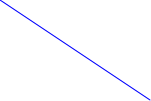
\includegraphics[scale=0.5]{videospiele/line1}|
(line -150 100 "blue")
|\evalsto| |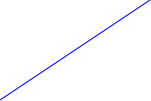
\includegraphics[scale=0.5]{videospiele/line2}|
\end{lstlisting}
%
Wir können auch ein Bild erzeugen, in dem Text steht, und zwar mit der
Funktion \lstinline{text}\indexvariable{text}, die folgende Signatur hat:
%
\begin{lstlisting}
(: text (string real color -> image))
\end{lstlisting}
%
Die Zahl ist die Höhe der Buchstaben.  Beispiel:
%
\begin{lstlisting}
(text "Schreibe Dein Programm!" 20 "red")
|\evalsto| |
\includegraphics[scale=0.5]{videospiele/text}|
\end{lstlisting}
%
Manchmal reichen einfache Rechtecke und Kreise nicht aus und wir
wollen komplexere Formen erzeugen.  Eine Möglichkeit ist die Funktion
\lstinline{polygon}\indexvariable{polygon}, die ein n-Eck
zeichnet.  Sie hat folgende Signatur:
%
\begin{lstlisting}
(: polygon ((list-of (mixed posn pulled-point)) mode color -> image)) 
\end{lstlisting}
%
Diese Funktion akzeptiert eine Liste von Eckpunkten und die üblichen
\lstinline{mode}- und \lstinline{color}"=Argumente.  Ein Eckpunkt 
muss entweder zur Signatur \lstinline{posn} oder zu
\lstinline{pulled-point} gehören.  Das sind eingebaute Record-Typen,
bei denen \lstinline{posn}\indexvariable{posn} so definiert sein könnte:
%
\indexvariable{posn}
\begin{lstlisting}
(define-record posn
  make-posn
  posn?
  (posn-x real)
  (posn-y real))
\end{lstlisting}
%
Dieser Typ definiert also ganz normale kartesische Koordinaten mit X-
und Y-Komponente.  Hier ist ein Beispiel für ein Polygon mit solchen
Eckpunkten:
%
\begin{lstlisting}
(polygon (list (make-posn 0 0)
               (make-posn -20 40)
               (make-posn 120 0)
               (make-posn -20 -40))
         "solid"
         "plum")
|\evalsto| |
\includegraphics[scale=0.5]{videospiele/polygon1}|
\end{lstlisting}
%
Bei \lstinline{posn}-Eckpunkten sind die Kanten also alles gerade
Linien.  Mit \lstinline{pulled-point}-Eckpunkten ist es möglich, die
Kanten zu Kurven zu machen.  Auch \lstinline{pulled-point} ist ein
Record-Typ:
%
\indexvariable{pulled-point}
\begin{lstlisting}
(define-record pulled-point
 make-pulled-point
 pulled-point?
 (pulled-point-lpull real)
 (pulled-point-langle real)
 (pulled-point-x real)
 (pulled-point-y real)
 (pulled-point-rpull real)
 (pulled-point-rangle real))
\end{lstlisting}
%
Wie \lstinline{posn} hat auch \lstinline{pulled-point} eine X- und
eine Y-Koordinate.  Außerdem gibt es jeweils zwei "<Pull">- und 
"<Angle">-Komponenten, die spezifizieren, wie die Kanten gebogen
werden.  Abbildung~\ref{fig:pulled-point} zeigt, wie das
funktioniert:  Für jeden Eckpunkt gibt es eine Kante vom
vorigen Punkt~-- die \emph{eingehende} Kante~-- und die Kante zum nächsten
Punkt~-- die \emph{ausgehende} Kante.

\begin{figure}[tb]
  \centering
  \def\svgwidth{0.4\textwidth}
  \input{videospiele/pulled-point.pdf_tex}
  \caption{Funktionsweise von \lstinline{pulled-point}}
  \label{fig:pulled-point}
\end{figure}
%
Die \lstinline{pulled-point-langle}-Komponente gibt den Winkel an, mit
dem die eingehende Kante gebogen wird, die
\lstinline{pulled-point-rangle}-Komponente den Winkel ist für die
ausgehende Kante zuständig.  Abbildung~\ref{fig:pulled-point} zeigt,
in welche Richtung \lstinline{langle} und \lstinline{rangle} die
beiden Kanten von Punkt Nummer~2 biegen: Die eingehende Kante kommt von Punkt~1 her, die
ausgehende Kante geht zu Punkt~3.  Die Komponenten
\lstinline{pulled-point-lpull} und \lstinline{pulled-point-rpull}
geben an, wieviel die Kanten verbogen werden auf einer Skala zwischen $0$ und $1$.
%
\begin{lstlisting}
(polygon (list (make-pulled-point 1/2 0 0 0 1/2 -20)
               (make-posn -20 40)
               (make-pulled-point 1/2 -20 120 0 1/2 20)
               (make-posn -20 -40))
         "solid"
         "plum")
|\evalsto| |
\includegraphics[scale=0.5]{videospiele/polygon2}|
\end{lstlisting}
%
\begin{figure}[tb]
  \centering
  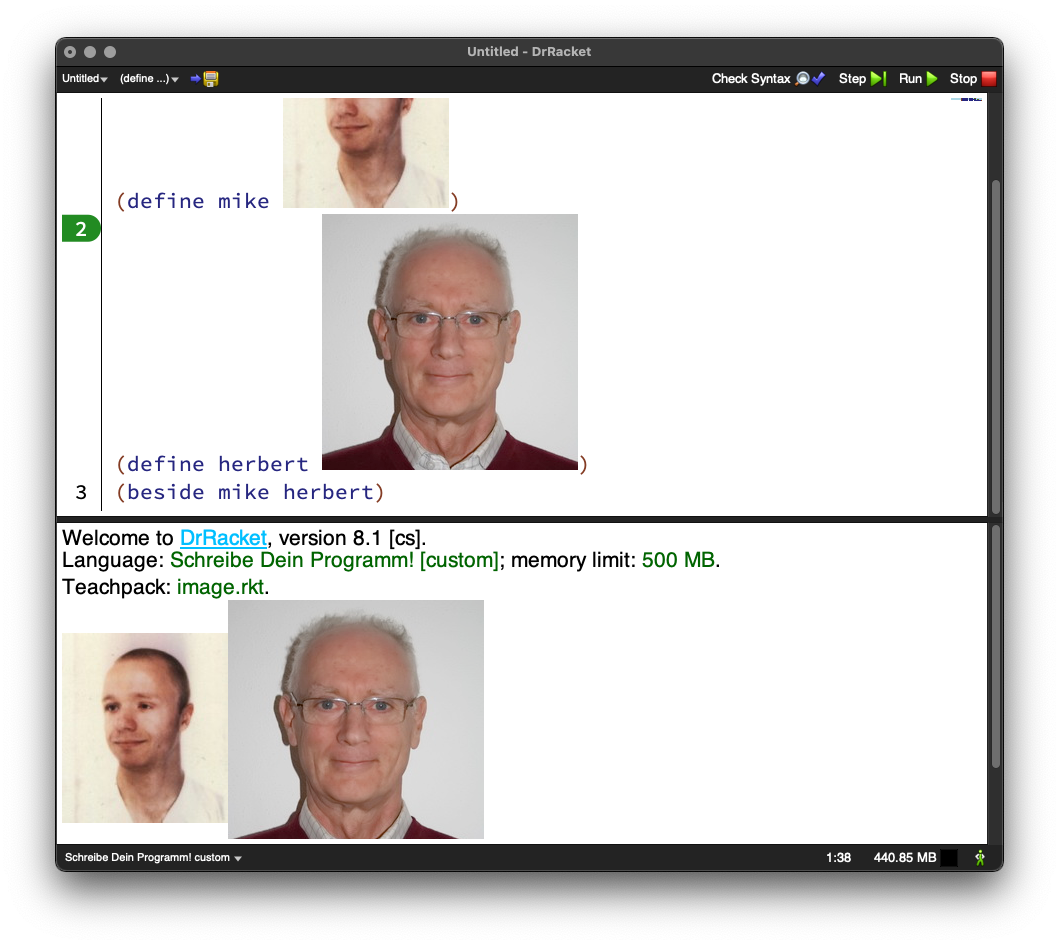
\includegraphics[height=0.4\textheight]{videospiele/insert-image}
  \caption{Bilddatei in Programm einbetten}
  \label{fig:image-insert}
\end{figure}
Es ist auch möglich, Bilder-Dateien in
\texttt{image.rkt}-Bilder zu verwandeln.  Das macht der Menüpunkt
\texttt{Bild einfügen} im \texttt{Spezial}-Menü.
Alternativ ist es möglich,
Bilder in anderen Applikationen auszuwählen und zu kopieren und dann
in DrRacket einzufügen.  Die eingefügten Bilder dienen dann als
Literale für Bild-Werte.  Abbildung~\ref{fig:image-insert} zeigt ein
Beispiel.

Schließlich ermitteln die folgenden Funktionen Breite und Höhe
eines Bildes:\indexvariable{image-width}\indexvariable{image-height}
%
\begin{lstlisting}
(: image-width  (image -> natural))
(: image-height (image -> natural))
\end{lstlisting}
%

\subsection{Bilder zusammensetzen und verändern}

Da diese geometrischen Formen für sich genommen langweilig sind,
können wir mehrere Bilder zu einem zusammensetzen.

Zum Aufeinanderlegen gibt es die Funktion
\lstinline{overlay}\indexvariable{overlay}, die ein Bild
mittig auf ein anderes Bild drauflegt.  Das Bild, das bei
\lstinline{overlay} herauskommt, ist groß genug, dass beide
Eingabebilder genau hineinpassen.  Signatur:
%
\begin{lstlisting}
(: overlay (image image -> image))
\end{lstlisting}
%
Beispiel:
%
\begin{lstlisting}
(overlay
  (circle 50 "solid" "gold")
  (rectangle 100 100 "solid" "blue"))
|\evalsto| |
\includegraphics[scale=0.5]{videospiele/overlay}|
\end{lstlisting}
%
Mittig ist nicht immer das richtige Arrangement für zwei Bilder, die
übereinandergelegt werden.  Die
Funktion~\lstinline{overlay/xy}\indexvariable{overlayxy}
erlaubt, das untere Bild gegenüber dem oberen in X- und Y-Richtung zu
verschieben.  Hier ist die Signatur:
%
\begin{lstlisting}
(: overlay/xy (image real real image -> image))
\end{lstlisting}
%
Beispiel:
%
\begin{lstlisting}
(overlay/xy
  (circle 50 "solid" "gold")
  10 -20
  (rectangle 100 100 "solid" "blue"))
|\evalsto| |
\includegraphics[scale=0.5]{videospiele/overlayxy}|
\end{lstlisting}
%
Das Beispiel zeigt, das auch \lstinline{overlay/xy} das Ergebnisbild
gerade so groß macht, dass die beiden Eingabebilder hineinpassen.

Manchmal macht auch \lstinline{overlay/xy} nicht das richtige, nämlich
wenn einfach nur ein Bild in eine "<Szene"> platziert werden soll,
zum Beispiel das Gürteltier auf einem Straßenabschnitt.  In dem Fall
wollen wir genau wie bei \lstinline{overlay/xy} kontrollieren, an
welchen Koordinaten das daraufgelegte Bild erscheint, aber das Bild
soll nicht größer werden, wenn zum Beispiel ein Teil des Gürteltiers
über den Straßenabschnitt hinausragt.  Diese Aufgabe erledigt die
Funktion
\lstinline{place-iamge}\indexvariable{place-image}, deren
Signatur der von \lstinline{overlay/xy} entspricht:
%
\begin{lstlisting}
(: place-image (image real real image -> image))
\end{lstlisting}
%
Die beiden Koordinaten werden allerdings anders als bei
\lstinline{overlay/xy} nicht relativ zur mittigen Anordnung
interpretiert.  Stattdessen geben die beiden Koordinaten die Position
im zweiten Bild an, wo die Mitte des ersten Bilds platziert wird,
ausgehend von der oberen linken Ecke des ersten Bildes.  Beispiel:
%
\begin{lstlisting}
(place-image
  (circle 50 "solid" "gold")
  40 70
  (rectangle 100 100 "solid" "blue"))
|\evalsto| |
\includegraphics[scale=0.5]{videospiele/place-image}|
\end{lstlisting}
%
Die Funktion \lstinline{place-image} hat noch eine große Schwester
\lstinline{place-image/align}.\indexvariable{place-image-align}\label{func:place-image-align}
Während \lstinline{place-image} den Bezugspunkt immer in der Mitte des
ersten Bilds setzt, erlaubt \lstinline{place-image} auch anderee
Bezugspunkte.  Hier die Signatur:
%
\begin{lstlisting}
(: place-image/align (image real real x-place y-place image -> image))
\end{lstlisting}
%
Die Signaturen \lstinline{x-place} und \lstinline{y-place} könnten
folgendermaßen definiert sein:
%
\indexvariable{x-place}
\indexvariable{y-place}
\begin{lstlisting}
(define x-place (signature (enum "left" "right" "center")))
(define y-place (signature (enum "top" "bottom" "center")))
\end{lstlisting}
%
Diese Argumente geben also an, ob der Bezugspunkt horizontal am linken
oder rechten Rand oder in der Mitte liegt und vertikal oben, unten
oder in der Mitte:
%
\begin{lstlisting}
(place-image/align
  (circle 20 "solid" "gold")
  40 70 "left" "center"
  (rectangle 100 100 "solid" "blue"))
|\evalsto| |
\includegraphics[scale=0.5]{videospiele/place-image-align1}|
(place-image/align
  (circle 20 "solid" "gold")
  40 70 "right" "center"
  (rectangle 100 100 "solid" "blue"))
|\evalsto| |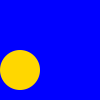
\includegraphics[scale=0.5]{videospiele/place-image-align2}|
(place-image/align
  (circle 20 "solid" "gold")
  40 70 "center" "center"
  (rectangle 100 100 "solid" "blue"))
|\evalsto| |
\includegraphics[scale=0.5]{videospiele/place-image-align3}|

(place-image/align
  (circle 20 "solid" "gold")
  40 70 "center" "top"
  (rectangle 100 100 "solid" "blue"))
|\evalsto| |
\includegraphics[scale=0.5]{videospiele/place-image-align4}|
(place-image/align
  (circle 20 "solid" "gold")
  40 70 "center" "bottom"
  (rectangle 100 100 "solid" "blue"))
|\evalsto| |
\includegraphics[scale=0.5]{videospiele/place-image-align5}|
\end{lstlisting}
%
Die folgenden Funktionen \lstinline{above} und \lstinline{beside}
kennst Du vielleicht noch aus dem ersten Kapitel auf
Seite~\pageref{function:beside-above}.  Sie setzten zwei Bilder
übereinander respektive nebeneinander:
% 
\begin{lstlisting}
(: above  (image image -> image))
(: beside (image image -> image))
\end{lstlisting}
%
Manchmal sieht ein Bild gut aus, ist aber zu klein oder zu groß
geraten.  Die Funktion \lstinline{scale} kann es größer oder kleiner
machen.  Signatur:
\begin{lstlisting}
(: scale (real image -> image))
\end{lstlisting}
%
Beispiel:
%
\begin{lstlisting}
(define c (circle 20 "solid" "green"))
(beside (scale 0.5 c)
        c
        (scale 1 c)
        (scale 1.5 c)
        (scale 2 c)
        (scale 3 c))
|\evalsto| |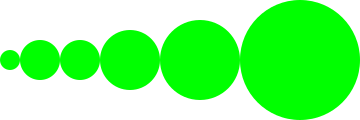
\includegraphics[scale=0.5]{videospiele/scale}|
\end{lstlisting}

\section{Modelle und Ansichten}

\mentioncode{videospiele/dillo-world.rkt}
%
In unserem Videospiel geht es um Gürteltiere auf dem texanischen
Highway.  Vielleicht erinnerst Du Dich, wir sind ihnen schon in
Abschnitt~\ref{sec:armadillo} auf Seite~\pageref{sec:armadillo}
begegnet.  Zur Erinnerung, hier ist der relevante Code dazu:
%
\indexvariable{run-over-dillo}
\indexvariable{dillo}
\begin{lstlisting}
; Ein Gürteltier hat folgende Eigenschaften:
; - Gewicht (in g)
; - lebendig oder tot
(define-record dillo
  make-dillo
  dillo?
  (dillo-weight natural)
  (dillo-alive? boolean))

(: make-dillo (natural boolean -> dillo))
(: dillo-weight (dillo -> natural))
(: dillo-alive? (dillo -> boolean))

(define dillo1 (make-dillo 55000 #t)) ; 55 kg, lebendig 
(define dillo2 (make-dillo 58000 #f)) ; 58 kg, tot
(define dillo3 (make-dillo 60000 #t)) ; 60 kg, lebendig
(define dillo4 (make-dillo 63000 #f)) ; 63 kg, tot

; Gürteltier überfahren
(: run-over-dillo (dillo -> dillo))

(define run-over-dillo
  (lambda (dillo)
    (make-dillo (dillo-weight dillo)
                #f)))
\end{lstlisting}
%
Die Datendefinition mit dem zugehörigen Code hält zwar einige Eigenschaften
von Gürteltieren fest, für ein Videospiel fehlt aber eine
grafische Darstellung.  Eine solche Repräsentation mit
zugehörigen Operationen heißt in der Softwararchitektur auch
\textit{Modell}\index{Modell} oder auch
\textit{Domänenlogik}\index{Domänenlogik}, und bei größeren Softwaresystemen
ist es eine gute Idee, das Modell von der grafischen Darstellung zu
trennen, damit das Modell stabil bleiben kann, auch wenn die grafische
Darstellung geändert wird.

Die grafische Darstellung eines Modells nennen wir dessen
\textit{Ansicht}\index{Ansicht} (auf englisch
\textit{View}\index{View}).  Wenn wir uns also mit Gürteltieren als
Modell für ein Videospiel beschäftigen, müssen wir daraus eine Ansicht
in Form eines Bildes berechnen.

Wir warnen Dich schonmal vor: Der grafische Gestaltung in diesem
Kapitel fehlt es an Finesse.  Wir hoffen, Du kannst
sie verbessern!

Die folgende Funktion macht aus einem \lstinline{dillo}-Wert ein Bild:
%
\begin{lstlisting}
; Gürteltier-Bild erzeugen
(: dillo-image (dillo -> image))
\end{lstlisting}
%
\begin{figure}[tb]
  \centering
  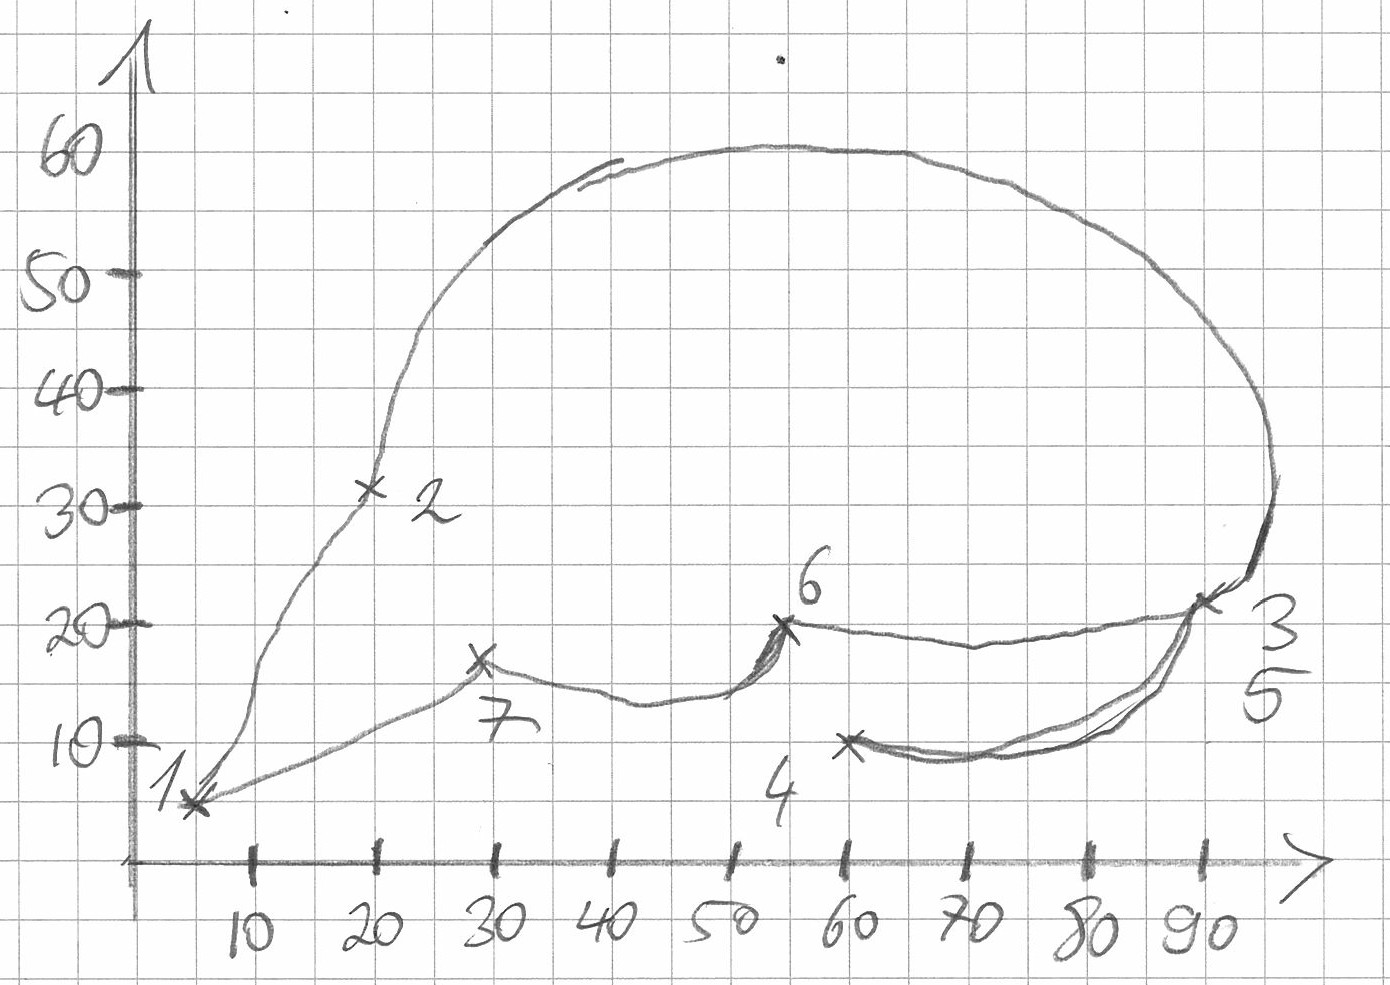
\includegraphics[width=0.6\textwidth]{videospiele/dillo}
  \caption{Umriss eines Gürteltiers}
  \label{fig:dillo-body}
\end{figure}
Als Basis dafür machen wir erstmal ein Bild mit dem Körper des
Gürteltiers.  Zu diesem Zweck haben wir in
Abbildung~\ref{fig:dillo-body} zunächst von Hand eine
Zeichnung mit dem Umriss des Gürteltiers in ein Koordinatensystem
gezeichnet und die Punkte markiert, an denen sich die Richtung des
Strichs abrupt ändert~-- also quasi die Ecken.  Diese Ecken haben wir
durchnummeriert und daraus haben wir dieses Polygon gemacht:
%
\indexvariable{dillo-body}
\begin{lstlisting}
(define dillo-body
  (overlay/xy (polygon
               (list (make-pulled-point 0.3 30
                                        5 (- 60 5)
                                        0.2 5)
                     (make-pulled-point 0.4 20
                                        20 (- 60 32)
                                        0.5 -70)
                     (make-pulled-point 0.5 120 
                                        90 (- 60 22)
                                        0.2 -30)
                     (make-pulled-point 0.5 90
                                        60 (- 60 10)
                                        0.5 90)
                     (make-pulled-point 0 0 
                                        90 (- 60 22)
                                        0.2 -30)
                     (make-pulled-point 0 0
                                        55 (- 60 20)
                                        0.3 -30)
                     (make-pulled-point 0 0
                                        29 (- 60 17)
                                        0.5 20))
               "solid"
               "brown")
              0 -30
              (rectangle 100 60
                         "solid" "transparent")))
\end{lstlisting}
%
Du siehst, da haben wir ganz schön viel herumprobiert, bis es
einigermaßen aussah, insbesondere bei den Zahlen für die
\lstinline{pulled-point}s.  Immerhin haben wir die Koordinaten aus der
Zeichnung direkt übertragen, dabei ist uns aber aufgefallen, dass die
Koordinaten in der Mathematik von unten nach oben, im Teachpack aber
von oben nach unten laufen.  Darum steht da zum Beispiel
\lstinline{(- 60 5)} für die Y-Koordinate 5, weil der obere Rand der
Zeichnung bei 60 liegt.

Außerdem ist das Gürteltier vor allem nach oben und rechts nach außen
gewölbt.  DrRacket schneidet das Polygon bei der Anzeige ab, weswegen
wir es mit \lstinline{overlay/xy} noch auf einen transparenten
Hintergrund montiert haben.  So sieht das Ergebnis aus:
%
\begin{lstlisting}
dillo-body
|\evalsto| |\includegraphics[scale=0.5]{videospiele/dillo-body}|
\end{lstlisting}
%
Jetzt wollen wir ja nicht jedes Gürteltier genau gleich darstellen,
sondern wir wollen dessen Eigenschaften bei der Darstellung
berücksichtigen.  Dafür schreiben wir die Funktion
\lstinline{dillo-image}, von der wir ja schon Kurzbeschreibung und
Signatur gesehen haben.  Hier ist das Gerüst mit der Schablone für
zusammengesetzte Daten als Eingabe:
%
\begin{lstlisting}
(define dillo-image
  (lambda (dillo)
    ... 
    (dillo-weight dillo)
    (dillo-alive? dillo)
    ...))
\end{lstlisting}
%
Wir sollten also noch berücksichtigen, wieviel das Gürteltier wiegt
und außerdem, ob es noch lebt.  Das Gewicht berücksichtigen wir, indem
wir das Gürteltier größer oder kleiner machen:
%
\begin{lstlisting}
(define dillo-image
  (lambda (dillo)
    (scale (+ 1
              (/ (- (dillo-weight dillo) 50000)
                 15000))
           dillo-body)
    ...
    (dillo-alive? dillo)
    ...))    
\end{lstlisting}
%
Den Faktor bei \lstinline{scale} haben wir durch Probieren
ermittelt.  Aber \lstinline{(dillo-alive? dillo)} steht noch da~-- wir
bauen das ein, indem wir einem toten Gürteltier "<tote Augen"> ins
Gesicht setzen:
%
\indexvariable{dillo-image}
\indexvariable{dead-eyes}
\begin{lstlisting}
(define dillo-image
  (lambda (dillo)
    (scale (+ 1
              (/ (- (dillo-weight dillo) 50000)
                 15000))
           (if (dillo-alive? dillo)
               dillo-body
               (overlay/xy dead-eyes
                           -25 -25
                           dillo-body)))))

(define dead-eyes
  (overlay (line 10 10 "green")
           (line -10 10 "green")))
\end{lstlisting}
%
Fertig ist die Gürteltier-Darstellung!

\section{Den Highway modellieren}
\label{sec:highway-model}

\begin{figure}[tb]
  \centering
  \includegraphics[height=0.4\textheight]{videospiele/dillo-world}
  \caption{Gürteltiere auf der Straße}
  \label{fig:dillo-world}
\end{figure}

Ein Gürteltier allein macht noch kein Videospiel: Wir setzen gleich
mehrere Gürteltiere auf die Straße und~-- natürlich~-- überfahren sie
dann.  Das sieht dann so aus wie in
Abbildung~\ref{fig:dillo-world}. Das Auto bewegt sich auf der Straße
und kann entweder auf die linke oder rechte Straßenseite wechseln, wo
es dann gegebenfalls über Gürteltiere fährt.  Oben links steht ein
Punktestand~-- wieviele Gürteltiere schon vom lebenden Zustand in den
toten überführt wurden.

Damit wir das alles darstellen können, müssen für alles
Datendefinition schreiben, was auf dem Bild der Straße zu sehen sind:
%
\begin{itemize}
\item die Position des Autos
\item die Positionen der Gürteltiere zusammen mit ihren Zuständen
\item der Punktestand
\end{itemize}
%
Für diese Aspekte des Spiels entwickeln wir Datendefinitionen.

Man sieht schon, dass "<Positionen"> eine wichtige Rolle spielen,
sowohl für das Auto als auch für die Gürteltiere.  In dem Bild kann
man sehen, dass dazu gehört, auf welcher Seite der Straße sich etwas
aufhält und bei welchem "<Straßenmeter">.  Dabei kommt folgende beiden
Datendefinitionen für die Straßenseite und eine Position heraus:
%
\indexvariable{side}
\indexvariable{position}
\begin{lstlisting}
; Straßenseite
(define side
  (signature (enum "left" "right")))

; Eine Position auf der Straße besteht aus:
; - Straßenmeter (Abstand vom Straßenanfang in Meter)
; - Seite
(define-record position
  make-position
  position?
  (position-m-from-start real)
  (position-side side))
\end{lstlisting}
%
Als nächstes müssen wir die Idee "<Positionen der Gürteltiere zusammen
mit ihren Zuständen"> in eine Datendefinition umwandeln.  Wir machen
das erstmal für ein einzelnes Gürteltier und nennen das Konzept
"<Gürteltier auf der Straße">:
%
\indexvariable{dillo-on-road}
\begin{lstlisting}
; Ein Gürteltier auf der Straße hat folgende Eigenschaften:
; - Gürteltier-Zustand
; - Position auf der Straße
(define-record dillo-on-road
  make-dillo-on-road
  dillo-on-road?
  (dillo-on-road-state dillo)
  (dillo-on-road-position position))
\end{lstlisting}
%

\section{Straßenansichten}

Jetzt wo wir die Welt modelliert haben können wir sie auch auf den
Bildschirm bringen.  Wir fangen erstmal mit den einfachen und
offensichtlichen Elementen an: der Straße Straße, inklusive der
Markierung auf dem Mittelstreifen und deme Auto.  Die Gürteltiere
haben wir ja schon.

Damit wir einigermaßen realistisch über die Proportionen von allem
nachdenken können, messen wir alles in Metern ab und wandeln zwischen
Metern und Pixeln hin und her.  Auf unserem Bildschirm sieht ein
Verhältnis von 1m:100 Pixel gut aus.  Diese Funktionen konvertieren
hin und her:

\indexvariable{meters->pixels}
\indexvariable{pixels->meters}
\begin{lstlisting}
; Meter in Pixel umwandeln
(: meters->pixels (real -> real))

(define meters->pixels
  (lambda (meters)
    (* meters 100)))

; Pixel in Meter umwandeln
(: pixels->meters (real -> real))

(define pixels->meters
  (lambda (pixels)
    (/ pixels 100)))
\end{lstlisting}
%
Die Straße selbst ist nur ein schwarzes Rechteck, das ist einfach.
Schwieriger sind die Straßenmarkierungen, also abwechselnd ein weißer
und ein schwarzer Streifen.  Damit das realistisch aussieht,
definieeren wir erst einmal die Länge der Markierungen und die der Lücken:
%
\indexvariable{marking-height}
\indexvariable{gap-height}
\begin{lstlisting}
(define marking-height 2) ; Höhe der Streifen
(define gap-height 1) ; Höhe der Lücken
\end{lstlisting}
%
Die Markierungen und die Lücken müssen wir abwechseln
aneinanderkleben.  Wie oft fragst Du?  Nun, der texanische Highway ist
unendlich lang, das wäre schwierig.  Aber wir zeigen ja nur einen
Ausschnitt, und darum machen wir nur soviele Streifen, wie in den
Ausschnitt passen.  Wieviele das sind, hängt von der Höhe des
Ausschnitts ab.  Wir könnten natürlich von Hand nachzählen, das würde
aber bedeuten, dass wir uns frühzeitig auf die Höhe des Ausschnitts
festlegen müssten.  Um das zu vermeiden, schreiben wir erst einmal
eine Funktion, die als Eingabe die Anzahl der Streifen akzeptiert.
Wir folgen der Schablone für Funktionen auf natürlichen Zahlen:
%
\indexvariable{markings}
\begin{lstlisting}
; Straßenmarkierung mit bestimmter Anzahl von Streifen malen
(: markings (natural -> image))

(define markings
  (lambda (n)
    (cond
      ((zero? n) empty-image)
      ((positive? n)
       (above (rectangle (meters->pixels .20)
                         (meters->pixels marking-height)
                         "solid"
                         "white")
              (rectangle (meters->pixels .20)
                         (meters->pixels gap-height)
                         "solid"
                         "black")
              (markings (- n 1)))))))
\end{lstlisting}
%
Hier jetzt die tatsächliche Höhe des Straßenabschnitts:
%
\indexvariable{road-window-height}
\begin{lstlisting}
(define road-window-height 12) ; Höhe des Straßenausschnitts
\end{lstlisting}
%
Die Idee ist, dass Du später nur diese eine Definition ändern musst, falls
Dir die Ausschnittshöhe nicht passt, und sich dann alles andere
automatisch anpasst.

Um die Anzahl der nötigen Markierungen zu berechnen, teilen wir die
Höhe des Straßenausschnitts durch die Länge einer Markierung plus
Lücke.  Zur Sicherheit addieren wir noch eins drauf: Die Division könnte
nicht ganz aufgehen.  Außerdem wird möglicherweise am Ende nur ein
Teil eines Streifens zu sehen sein, auch dafür ist es gut, wenn im
Zweifelsfall einer mehr da ist.
%
\indexvariable{marking-count}
\begin{lstlisting}
; Anzahl der nötigen Markierungen
(define marking-count
  (+ 1
     (quotient road-window-height
               (+ marking-height gap-height))))
\end{lstlisting}
%
Aus der Zahl machen wir schließlich
das Bild der Streifen:
%
\indexvariable{visible-markings}
\begin{lstlisting}
; sichtbare Markierungen
(define visible-markings
  (markings marking-count))
\end{lstlisting}
%
Zur Erinnerung: Die Funktion \lstinline{quotient} haben wir auf
Seite~\pageref{func:quotient} eingeführt, sie teilt ganzzahlig.

Nun können wir das Bild des Straßenausschnitts zusammensetzen.  Wir
brauchen neben der Höhe auch noch die Breite und machen erstmal eine
leere Szene nur aus schwarzem Asphalt:
%
\indexvariable{road-width}
\indexvariable{blank-road-window}
\begin{lstlisting}
; in Meter
(define road-width 5)

(define blank-road-window
  (empty-scene (meters->pixels road-width)
               (meters->pixels road-window-height)
               "black"))
\end{lstlisting}
%
Wie Mittelstreifen auf dem Straßenausschnitt platziert werden, hängt
davon ab, an welchem Straßenmeter sich der Bildausschnitt befindet.
Wir schreiben also eine Funktion, welche die Straßenmeter akzeptiert
und ein passendes Bild liefert:
\begin{lstlisting}
; Straßenausschnitt anzeigen
(: road-window (real -> image))
\end{lstlisting}
%
Wir benutzen \lstinline{place-image/align} (siehe
Seite~\pageref{func:place-image-align}), um die Mittelstreifen auf den
Asphalt zu setzen:
%
\begin{lstlisting}
(define road-window
  (lambda (meters)
    (place-image/align visible-markings
                       ...
                       ...
                       ... ...
                       blank-road-window)))
\end{lstlisting}
%
Wir setzen zunächst den Bezugspunkt beim Mittelstreifen nach oben in
die Mitte:
%
\begin{lstlisting}
(define road-window
  (lambda (meters)
    (place-image/align visible-markings
                       ...
                       ...
                       "center" "top"
                       blank-road-window)))
\end{lstlisting}
%
In X-Richtung muss der Mittelstreifen in die Mitte, da können wir
einfach die Breite der Straße halbieren.

Bei der Y-Koordinate ist es schwieriger: Die hängt von den
Straßenmetern ab.  Die Straßenmeter sind aber (außer ganz am Anfang)
mehr als der Ausschnitt hoch beziehungsweise das Mittelstreifenbild
lang ist.  Das Mittelstreifenbild wiederholt sich aber immer, wenn ein
Streifen plus Lücke vorbeigezogen ist.  Wir rechnen also die Anzahl
der Pixel dafür aus:
%
\indexvariable{marking-segment-pixels}
\begin{lstlisting}
(define marking-segment-pixels
  (meters->pixels (+ marking-height gap-height)))
\end{lstlisting}
%
Durch diese Zahl teilen wir und nehmen den Divisionsrest, um die
Y-Position zu bekommen.  Das heißt nicht ganz~-- der Divisionsrest ist immer
positiv, und damit ist der Mittelstreifen zu weit unten: Wir ziehen
das Bild noch um einen Streifen nach oben, indem wir
\lstinline{marking-segment-pixels} abziehen.  Das kommt dabei heraus:
%
\indexvariable{road-window}
\begin{lstlisting}
(define road-window
  (lambda (meters)
    (place-image/align visible-markings
                       (/ (image-width blank-road-window) 2)
                       (- (remainder (meters->pixels meters)
                                     marking-segment-pixels)
                          marking-segment-pixels)
                       "center" "top"
                       blank-road-window)))
\end{lstlisting}
%
\begin{aufgabeinline}
  Probiere \lstinline{road-window} aus.  Entferne die Substraktion von
  \lstinline{marking-segment-pixels} und untersucht, wie sich das
  auswirkt!
\end{aufgabeinline}
%

\section{Bewegte Bilder mit \texttt{universe.rkt}}

Bisher haben wir nur statische, langweilige Bilder.  Es ist Zeit, sie
in Bewegung zu setzen.  Dafür brauchen wir ein weiteres Teachpack
namens \texttt{universe.rkt}.  Um es zu aktivieren, musst Du nochmal
ins \texttt{Sprache}/\texttt{Language}-Menü und dort auf
\texttt{Teachpack hinzufügen}/\texttt{Add Teachpack} drücken und in
dem dann auftauchenden Dialog auf \texttt{universe.rkt} und
schließlich auf \texttt{OK} drücken.

Zum \texttt{universe.rkt}-Teachpack gehört eine Funktion namens
\lstinline{animate}\indexvariable{animate}.  Was sie macht,
verdeutlicht am einfachsten ein Beispiel, dass Du in die REPL
eintippen kannst:
%
\begin{lstlisting}
(animate
  (lambda (ticks)
     (place-image/align (circle 5 "solid" "red") 
                        100 ticks "center" "top" 
                        (square 200 "solid" "black"))))
\end{lstlisting}
%
\begin{aufgabeinline}
  Probier es aus!
\end{aufgabeinline}
%
Du siehst einen kleinen roten Kreis sich in einem quadratischen Bild
von oben nach unten bewegen. 

Die neue Funktion \lstinline{animate} akzeptiert eine Funktion mit
einer Eingabe names \lstinline{ticks}, die ein Bild produziert:
%
\begin{lstlisting}
(: animate ((natural -> image) -> natural))
\end{lstlisting}
%
\lstinline{Animate} ruft die Funktion 28mal in der Sekunde auf und
zeigt die entstehenden Bilder hintereinander als Animation an.  Dabei
übergibt \lstinline{animate} als \lstinline{ticks} eine natürliche
Zahl, die bei Null anfängt, und jedesmal um eins größer wird: Sie
misst also die Zeit, in sogenannten \textit{Ticks}\index{Ticks}.

Wir benutzen jetzt \lstinline{animate}, um das Bild des
Straßenausschnitts in Bewegung zu setzen~-- so, dass das Wagen genau
in der Mitte ist.  Wir legen zuerst fest, wie schnell der Wagen fährt.
Wir haben uns für ein recht gemächliches Tempo entschieden, damit wir auch
wirklich alle Gürteltiere erwischen:
%
\indexvariable{meters-per-tick}
\begin{lstlisting}
; Meter pro Tick
(define meters-per-tick 0.1)
\end{lstlisting}
%
Diese Funktion ist so einfach, dass sich ausnahmsweise separates
Testen nicht lohnt:
%
\indexvariable{ticks->meters}
\begin{lstlisting}
; Ticks in Meter umwandeln
(: ticks->meters (natural -> rational))

(define ticks->meters
  (lambda (ticks)
    (* meters-per-tick ticks)))
\end{lstlisting}
%
Damit können wir eine Funktion schreiben, die aus Ticks Straßenmeter
macht und \lstinline{road-window} aufruft:
%
\indexvariable{road-window-at-ticks}
\begin{lstlisting}
; Straßenausschnitt zu Zeitpunkt anzeigen
(: road-window-at-ticks (natural -> image))

(define road-window-at-ticks
  (lambda (ticks)
    (road-window (ticks->meters ticks))))
\end{lstlisting}
% Du kannst
also folgendes ausprobieren:
%
\begin{lstlisting}
(animate road-window-at-ticks)
\end{lstlisting}
%
\begin{aufgabeinline}
  Schreibe eine andere Funktion Deiner Wahl mit der für
  \lstinline{animate} passenden Signatur und probiere
  \lstinline{animate} damit aus!
\end{aufgabeinline}

\section{Autos und Gürteltiere auf dem Highway}

Die Straße ist fertig, als nächstes ist das Auto dran.  Wir fangen mit
einem Rad an:
%
\indexvariable{wheel}
\begin{lstlisting}
; Rad
(define wheel
  (rectangle (meters->pixels 0.2) (meters->pixels .5)
             "outline" "white"))
\end{lstlisting}
%
Als nächstes setzen wir zwei Räder zu einem Bild zusammen, das dann
links und rechts von der Karosserie platziert werden:
%
\indexvariable{wheels-on-one-side}
\indexvariable{car-width}
\indexvariable{car-length}
\indexvariable{car}
\begin{lstlisting}
; Zwei Räder auf einer Seite des Autos
(define wheels-on-one-side
  (above wheel
         (rectangle 0 (meters->pixels 1.2) "solid" "black")
         wheel))

; Breite des Autos
(define car-width 1.5)
; Länge des Autos
(define car-length 3.0)
 
; Bild des Autos
(define car
  (beside
   wheels-on-one-side
   (rectangle (meters->pixels car-width) (meters->pixels car-length)
              "solid" "blue")
   wheels-on-one-side))
\end{lstlisting}
%
Schließlich müssen wir Auto und auch die Gürteltiere noch auf der
Straße platzieren.  Wir müssen erstmal überlegen, welche Signatur die
Funktion überhaupt hat.  Klar ist, dass ein Bild herauskommen soll.
Als Eingaben stehen schon einmal fest:
%
\begin{itemize}
\item das Bild, das auf der Straße platziert werden soll
\item die Position des Bildes
\end{itemize}
%
Wir benötigen außerdem noch:
%
\begin{itemize}
\item die Zeit, weil sie bestimmt, welcher Ausschnitt der Straße
  angezeigt wird
\item das Bild der Straße
\end{itemize}
%
Letzteres überrascht Dich vielleicht. Ist das Bild der Straße nicht
immer das gleiche?  Nein, ist es nicht!  Zunächst einmal ist die
Position des Mittelstreifens je nach Zeit immer unterschiedlich.
Außerdem wollen wir ja nicht nur ein Bild auf der Straße platzieren,
sondern viele.  Dafür füttern wir das Ergebnis der Funktion wieder in
die Funktion hinein, um ein weiteres Bild zu platzieren.

Kurzbeschreibung, Signatur und Gerüst sehen entsprechend aus wie
folgt:
%
\begin{lstlisting}
; Bild auf der Straße platzieren
(: place-image-on-road (image natural image position -> image))

(define place-image-on-road
  (lambda (road-image ticks image position)
    ...))
\end{lstlisting}
%
Da es sich bei \lstinline{position} um zusammengesetzte Daten handelt,
stehen in der Schablone Aufrufe der Selektoren:
%
\begin{lstlisting}
(define place-image-on-road
  (lambda (road-image ticks image position)
    ...
    (position-m-from-start position)
    (position-side position)
    ...))
\end{lstlisting}
%
Wir müssen jetzt die Pixelkoordinaten des Bildes relativ zum
Straßenausschnitt berechnen.  Bei der X-Koordinate ist das
verhältnismäßig einfach.  Wir legen eine Variable 
\lstinline{pixels-from-left} an, die sich aus 
\lstinline{(position-side position))} ergibt, 
was schon in der Schablone steht.  Die Seite
ist relativ zum Mittelstreifen, für dessen X-Koordinate wir ebenfalls
eine Zwischenvariable anlegen:
%
\begin{lstlisting}
    ; X-Koordinate der Mitte der Straße, in Pixeln
    (define middle-pixels (/ (image-width road-image) 2))
\end{lstlisting}
%
Daraus ergibt sich \lstinline{pixels-from-left} so:
%
\begin{lstlisting}
    ; X-Koordinate des Mittelpunkts des Bilds
    (define pixels-from-left
      (cond
        ((string=? (position-side position) "left")
         (* middle-pixels 0.5)) ; Mitte der linken Spur
        ((string=? (position-side position) "right")
         (* middle-pixels 1.5)))) ; Mitte der rechten Spur
\end{lstlisting}
%
Als nächstes brauchen wir die Y-Koordinate, da ist es etwas
komplizierter: Wir benötigen die Y-Koordinate von \lstinline{image}
\emph{relativ} zum unteren Rand des Bildes.  (Oder des oberen, das
geht auch.)  Das wäre folgender Ausdruck:
%
\begin{lstlisting}
(- (position-m-from-start position)
   (ticks->meters ticks))
\end{lstlisting}
%
Diese Koordinate ist noch in Metern, die müssen wir noch in Pixel
umrechnen.  Außerdem müssen wir berücksichtigen, dass die
Pixel-Koordinaten von oben nach unten laufen, die Straßenmeter aber
von unten nach oben~-- wir ziehen also diese Zahl von der Höhe des
Bildes ab.  Damit können wir wieder einmal
\lstinline{place-image/align} (siehe
Seite~\pageref{func:place-image-align}) bemühen, um das Bild auf die
Straße zu setzen.  Die Funktion sieht vollständig so aus:
%
\indexvariable{place-image-on-road}
\begin{lstlisting}
(define place-image-on-road
  (lambda (road-image ticks image position)
    ; X-Koordinate der Mitte der Straße, in Pixeln
    (define middle-pixels (/ (image-width road-image) 2))
    ; X-Koordinate des Mittelpunkts des Bilds
    (define pixels-from-left
      (cond
        ((string=? (position-side position) "left")
         (* middle-pixels 0.5)) ; Mitte der linken Spur
        ((string=? (position-side position) "right")
         (* middle-pixels 1.5)))) ; Mitte der rechten Spur

    (place-image/align
     image
     pixels-from-left
     (- (image-height road-image)
        (meters->pixels (- (position-m-from-start position)
                           (ticks->meters ticks))))
     "center" "center"
     road-image)))
\end{lstlisting}
%
Die Funktion ist kompliziert genug, dass wir sie testen sollten.
Einen \lstinline{check-expect}-Test vorab zu konstruieren ist schier
unmöglich, aber wir können die Funktion zumindest in der REPL
ausprobieren, am einfachsten bei 0 Ticks, also am Anfang des Spiels:
%
\begin{lstlisting}
(place-image-on-road (road-window 0) 0 car (make-position 0 "left"))
|\evalsto{} \includegraphics[height=1.5cm]{videospiele/car-bottom}
\end{lstlisting}
%
Da ist noch ein Problem!  Das Auto ist am unteren Rand und nur zur
Hälfte zu sehen, wir wollen es aber gern in der Mitte.  Wir müssen
also noch die Hälfte der Höhe des Straßenabschnitts abziehen,
entsprechend den Aufruf von \lstinline{place-image/align} korrigieren:
%
\begin{lstlisting}
  (place-image/align
     image
     pixels-from-left
     (- (image-height road-image)
        (meters->pixels (+ (- (position-m-from-start position)
                              (ticks->meters ticks))
                           (/ road-window-height 2))))
     "center" "center"
     road-image)
\end{lstlisting}
%
Jetzt ist alles bei $0$ in der Mitte!

Diese Funktion können wir jetzt benutzen, um zunächst das Autobild auf
dem Straßenabschnitt zu platzieren:
% 
\indexvariable{place-car-on-road}
\begin{lstlisting}
; Auto auf die Straße setzen
(: place-car-on-road (natural position image -> image))
                      
(define place-car-on-road
  (lambda (ticks car-position road-image)
    (place-image-on-road road-image
                         ticks
                         car car-position)))
\end{lstlisting}
%
\begin{aufgabeinline}
  Konstruiere auf Basis von \lstinline{place-car-on-road} eine
  Funktion, die Du an \lstinline{animate} übergeben kannst und
  probiere sie aus!
\end{aufgabeinline}
%
Ähnlich machen wir das für das Gürteltier-Bild.  Die nötigen Angaben,
zu Position und Zustand des Gürteltiers ziehen wir aus dem
\lstinline{dillo-on-road}-Record:
%
\begin{lstlisting}
; Ein Tier auf die Straße malen
(: place-dillo-on-road (natural dillo-on-road image -> image))

(define place-dillo-on-road
  (lambda (ticks dillo-on-road road-image)
    (place-image-on-road road-image
                         ticks
                         (dillo-image (dillo-on-road-state dillo-on-road))
                         (dillo-on-road-position dillo-on-road))))
\end{lstlisting}
%
Jetzt gibt es ja auf der Straße nicht nur ein Gürteltier sondern
viele, die als Liste im \lstinline{world}-Record stecken.  Dafür
brauchen wir eine Funktion mit folgender Kurzbeschreibung und
Signatur:
%
\begin{lstlisting}
; Alle Tiere auf die Straße malen
(: place-dillos-on-road
   (natural (list-of dillo-on-road) image -> image))
\end{lstlisting}
%
Wir könnten das nach Konstruktionsanleitung für Listen programmieren.
Einfacher ist aber, die universelle Funktion~\lstinline{fold} zu
benutzen. (Siehe Abschnitt~\ref{sec:fold} auf
Seite~\pageref{sec:fold}.)  Das sieht dann so aus:
%
\indexvariable{place-dillos-on-road}
\begin{lstlisting}
(define place-dillos-on-road
  (lambda (ticks dillos-on-road road-image)
    (fold road-image
          (lambda (dillo-on-road image)
            (place-dillo-on-road ticks dillo-on-road image))
          dillos-on-road)))
\end{lstlisting}
%
Neben Auto und Gürteltieren fehlt noch die Punktzahl oben links in der
Ecke.  Das erledigt folgende Funktion:
%
\indexvariable{place-score}
\begin{lstlisting}
; Punktzahl anzeigen
(: place-score (natural image -> image))

(define place-score
  (lambda (score image)
    (place-image/align
     (text (number->string score) 100 "blue")
     0 0
     "left" "top"
     image)))
\end{lstlisting}
%

\section{Die Welt ein Highway}

Es wird Zeit, dass wir alles zusammensetzen zu einem Spiel, das sich
bewegt und dass auf Knopfdruck reagiert.  Das
\texttt{universe.rkt}-Teachpack fordert, dass wir eine Datendefinition
erstellen, in der der gesamte Zustand des Spiels stecks.  In
Abschnitt~\ref{sec:highway-model} auf
Seite~\pageref{sec:highway-model} hatten wir schon folgende Aspekte
aufgelistet:
%
\begin{itemize}
\item die Position des Autos
\item die Positionen der Gürteltiere zusammen mit ihren Zuständen
\item der Punktestand
\end{itemize}
%
Wir wissen, dass uns das \texttt{universe.rkt}-Teachpack später die
Zeit als Ticks liefern wird: Daraus können wir die Straßenmeter der
Position des Autors berechnen.  Nur noch die Seite müssen wir explizit
repräsentieren.  Es entsteht also folgende etwas angepasste Datendefinition:
%
\indexvariable{world}
\begin{lstlisting}
; Die Welt des Spiels besteht aus:
; - Ticks seit Spielanfang
; - Seite, auf der das Auto fährt
; - Tiere auf der Straße
; - Punktzahl
(define-record world
  make-world
  world?
  (world-ticks natural)
  (world-car-side side)
  (world-dillos-on-road (list-of dillo-on-road))
  (world-score natural))
\end{lstlisting}
%
Hier ein Beispiel dafür:
%
\indexvariable{dillos-on-road}
\indexvariable{initial-world}
\begin{lstlisting}
; Vier Gürteltiere auf der Straße
(define dillos-on-road
  (list (make-dillo-on-road dillo1 (make-position 20 "left"))
        (make-dillo-on-road dillo2 (make-position 26 "right"))
        (make-dillo-on-road dillo3 (make-position 30 "left"))
        (make-dillo-on-road dillo4 (make-position 42 "left"))))

; Welt am Anfang, Auto steht links
(define initial-world
  (make-world 0 "left" dillos-on-road 0))
\end{lstlisting}
%
Wir werden für \lstinline{place-car-on-road} die Position des Autos
als \lstinline{position}-Record benötigen, die noch nicht direkt im
\lstinline{world}-Record vorhanden ist.  Die Seite steht immerhin
schon da.  Die Straßenmeter berechnen wir aus den Ticks.  Die Funktion
dafür hat Kurzbeschreibung, Signatur und Testfälle wie folgt:
%
\begin{lstlisting}
; Position des Autos
(: world-car-position (world -> position))

(check-expect (world-car-position (make-world 0 "left" empty 0))
              (make-position 0 "left"))
(check-expect (world-car-position (make-world 100 "right" empty 0))
              (make-position (ticks->meters 100) "right"))
\end{lstlisting}
%
Die Schablone für die Funktion berücksichtigt, dass es sich sowohl bei
Ein- als auch bei der Ausgabe jeweils um zusammengesetzte Daten handelt:
%
\begin{lstlisting}
(define world-car-position
  (lambda (world)
    (make-position ... ...)
    ...
    (world-ticks world)
    (world-car-side world)
    (world-dillos-on-road world)
    (world-score world)
    ...))
\end{lstlisting}
%
Nur die ersten beiden Felder von \lstinline{world} sind relevant für
die Position des Autos~-- Gürteltiere und Punktzahl sind sichtlich
nicht relevant.  Für die Position brauchen wir die Straßenmeter, die
wir aus den Ticks mit Hilfe von \lstinline{ticks->meters} berechnen
können:
%
\indexvariable{world-car-position}
\begin{lstlisting}
(define world-car-position
  (lambda (world)
    (make-position (ticks->meters (world-ticks world))
                   (world-car-side world))))
\end{lstlisting}
%
Jetzt haben wir endlich alle Funktionen, die wir benötigen, um die
ganze Welt anzuzeigen.  Wir müssen sie nur kombinieren, um alles in
einem \lstinline{world}-Record als Straßenabschnitt anzuzeigen:
%
\indexvariable{world->image}
\begin{lstlisting}
; Spiel anzeigen
(: world->image (world -> image))

(define world->image
  (lambda (world)
    (define ticks (world-ticks world))
    (place-score
     (world-score world)
     (place-car-on-road
      ticks
      (world-car-position world)
      (place-dillos-on-road
       ticks
       (world-dillos-on-road world)
       (road-window ticks))))))
\end{lstlisting}
%
Du kannst jetzt natürlich
\lstinline{(world->image initial-world)}
ausprobieren, aber da ist nur der anfängliche, leere Straßenabschnitt
zu sehen.

Besser wird es mit \lstinline{animate}.  Dafür brauchen wir eine
Funktion mit Signatur \lstinline{(natural -> image)}.  Da wir schon
\lstinline{world->image} mit der Signatur \lstinline{(world -> image)}
haben, brauchen wir noch eine Funktion mit Signatur
\lstinline{(natural -> world)}, die einen passenden
\lstinline{world}-Wert erzeugt:
%
\indexvariable{world-at-ticks}
\begin{lstlisting}
; Statische Welt zu einem bestimmten Zeitpunkt darstellen
(: world-at-ticks (natural -> world))

(define world-at-ticks
  (lambda (ticks)
    (make-world ticks "left" dillos-on-road 0)))
\end{lstlisting}
%
Nun können wir \lstinline{animate} mit einer Kombination aus den
beiden aufrufen:
%
\begin{lstlisting}
(animate (lambda (ticks) (world->image (world-at-ticks ticks))))
\end{lstlisting}
%
Da sieht man die Straße vorbeiziehen, und schließlich tauchen auch
Gürteltiere auf.  Aber das Auto ist links festgeklebt und die
Gürteltiere sterben auch nicht, wenn das Auto drüberfährt.

\section{Überfahren konkret}
  
Was fehlt noch, damit aus dem
\lstinline{world}-Record alle Aspekte des Spiels berechnet werden
können, mithin der texanische Highway simuliert:\label{page:dillo-world-todos}
%
\begin{enumerate}
\item Wir müssen feststellen ob das Auto die Position eines
  Gürteltiers berührt und dieses damit überfährt.
\item Wir müssen zählen, wieviele Tiere vo einem gegebenen
  Zeitpunkt vom Auto touchiert, mithin überfahren werden, damit wir
  die Punktzahl entsprechend erhöhen können.
\item Schließlich müssen wir alle Tiere überfahren, deren Position
  unter das Auto gerät.
\end{enumerate}
%
Diese Liste arbeiten wir in diesem Abschnitt ab.
%
\paragraph{Berührung eines Gürteltiers} Als nächstes auf der Liste auf
Seite~\pageref{page:dillo-world-todos} müssen wir feststellen, ob das
Auto die Position eines Gürteltiers berührt.

Wir brauchen eine Funktion mit Kurzbeschreibung und Signatur wie
folgt:
%
\begin{lstlisting}
; Berührt das Auto eine Position?
(: car-on-position? (position position -> boolean))
\end{lstlisting}
%
Das Auto berührt eine Position, wenn die Position auf der gleichen
Straßenseite nah dran ist.  Hier die Testfälle dazu:
%
\begin{lstlisting}
(check-expect (car-on-position? (make-position 10 "left")
                                (make-position 10 "right"))
              #f)
(check-expect (car-on-position? (make-position 10 "left")
                                (make-position 10 "left"))
              #t)
(check-expect (car-on-position? (make-position 11 "left")
                                (make-position 10 "left"))
              #t)
(check-expect (car-on-position? (make-position 10 "left")
                                (make-position 11 "left"))
              #t)
\end{lstlisting}
%
Für die Schablone haben wir es bei beiden Eingaben mit
zusammengesetzten Daten zu tun:
%
\indexvariable{car-on-position?}
\begin{lstlisting}
(define car-on-position?
  (lambda (car-position position)
    ...
    (position-side car-position) 
    (position-side position)
    (position-m-from-start car-position)
    (position-m-from-start position)
    ...))
\end{lstlisting}
%
Die beiden Straßenseiten müssen gleich sein.  Bei den Straßenmetern
der beiden Positionen ist relevant, dass die Straßenmeter des Autos
genau in der Mitte des Autos sind~-- die Position darf nicht mehr als
die Hälfte davon entfernt sein.  Um den Vergleich zu erleichtern, egal
ob die Position vor oder hinter dem Mittelpunkt ist, benutzen wir die
eingebaute Funktion \lstinline{abs}\indexvariable{abs}.\label{func:abs}  Diese
Funktion berechnet den \textit{Absolutbetrag}\index{Absolutbetrag}
einer Zahl: Sie macht aus negativen Zahlen die entsprechenden
positiven Zahlen:
%
\begin{lstlisting}
(abs 5)
|\evalsto| 5
(abs -5)
|\evalsto| 5
\end{lstlisting}
%
Hier die fertige Funktion:
%
\begin{lstlisting}
(define car-on-position?
  (lambda (car-position position)
    (and (string=? (position-side car-position) 
                   (position-side position))
         (<= (abs (- (position-m-from-start car-position)
                     (position-m-from-start position)))
             (/ car-length 2)))))
\end{lstlisting}

\paragraph{Wieviele Tiere sind gerade unter dem Auto?} Als nächstes
schreiben wir eine Funktion, welche die Tiere unter dem Auto zählt,
damit wir die Punktzahl entsprechend erhöhen können.  Genauer gesagt
zählen wir nur die \emph{lebendigen} Gürteltiere: Für das nochmalige
Überfahren eines toten Gürteltiers gibt es keinen Punkt.  Hier
Kurzbeschreibung und Signatur:
%
\begin{lstlisting}
; Wieviele Tiere werden vom Auto berührt?
(: live-dillos-under-car-count 
   (position (list-of dillo-on-road) -> natural))
\end{lstlisting}
%
Für den Test sollten wir in der Eingabe sowohl lebendige als auch
tote Gürteltiere unterbringen, ebenso wie solche, die unter dem Auto
liegen, und solche, die weiter weg sind:
%
\begin{lstlisting}
(check-expect
  (live-dillos-under-car-count
    (make-position 10 "left")
     (list (make-dillo-on-road dillo1 (make-position 10 "left"))
           (make-dillo-on-road dillo2 (make-position 10 "right"))
           (make-dillo-on-road dillo2 (make-position 11 "left"))
           (make-dillo-on-road dillo1 (make-position 9 "left"))
           (make-dillo-on-road dillo1 (make-position 12 "left"))))
  2)
\end{lstlisting}
%
Der Test zählt das erste und das vorletzte Gürteltier.

Für die Definition könnten wir die Schablone für Funktionen auf Listen
heranziehen.  Da es aber darum geht, aus einer Liste einige Elemente
auszuwählen, die einem bestimmten Kriterium entsprechen, können wir
auch die Funktion \lstinline{filter} von Seite~\pageref{func:filter}
benutzen, die eingebaute Version von \lstinline{extract-list}.  Damit
extrahieren wir die zu zählenden Gürteltiere.  Die müssen wir nur noch
mit der ebenfalls eingebauten Funktion~\lstinline{length}
zählen. (\lstinline{Length} ist die eingebaute Version von
\lstinline{list-length}, siehe Seite~\pageref{func:length}.)
%
\indexvariable{live-dillos-under-car-count}
\begin{lstlisting}
(define live-dillos-under-car-count
  (lambda (car-position dillos-on-road)
    (length
     (filter (lambda (dillo-on-road)
               (and (car-on-position?
                       car-position
                       (dillo-on-road-position dillo-on-road))
                    (dillo-alive? 
                      (dillo-on-road-state dillo-on-road))))
             dillos-on-road))))
\end{lstlisting}

\paragraph{Gürteltiere tatsächlich überfahren} Als letzter
Arbeitsauftrag bleibt noch, die Gürteltiere, die vom Auto touchiert
werden, vom lebenden in den toten Zustand zu überführen.  Die Funktion
akzeptiert wie \lstinline{live-dillos-under-car-count} die Position
des Autos und die Gürteltiere:
%
\begin{lstlisting}
; Alle Tiere überfahren, die das Auto berührt
(: run-over-dillos-on-road
   (position (list-of dillo-on-road) -> (list-of dillo-on-road)))
\end{lstlisting}
%
Beim Testen gibt es jede Menge tote Gürteltiere, darum definieren wir
den dazugehörigen Zustand zwecks Wiederverwendung:
%
\begin{lstlisting}
(define dead-dillo1 (run-over-dillo dillo1))

(check-expect
 (run-over-dillos-on-road
  (make-position 10 "left")
  (list (make-dillo-on-road dillo1 (make-position 10 "left"))
        (make-dillo-on-road dillo1 (make-position 10 "right"))
        (make-dillo-on-road dillo1 (make-position 11 "left"))
        (make-dillo-on-road dillo1 (make-position 9 "left"))
        (make-dillo-on-road dillo1 (make-position 12 "left"))))
 (list (make-dillo-on-road dead-dillo1 (make-position 10 "left"))
       (make-dillo-on-road dillo1 (make-position 10 "right"))
       (make-dillo-on-road dead-dillo1 (make-position 11 "left"))
       (make-dillo-on-road dead-dillo1 (make-position 9 "left"))
       (make-dillo-on-road dillo1 (make-position 12 "left"))))
\end{lstlisting}
%
Die Funktion wendet also eine Operation auf jedes Element der Liste an
und gibt uns die Ergebnisse in einer Liste zurück: Dafür können wir
wieder eine Higher"=Order"=Funktion aus Kapitel~\ref{cha:higher-order}
verwenden, nämlich \lstinline{map}, die eingebaute Version von
\lstinline{list-map}, siehe Seite~\pageref{func:map}.
%
\begin{lstlisting}
(define run-over-dillos-on-road
  (lambda (car-position dillos-on-road)
    (map (lambda (dillo-on-road)
           ...)
         dillos-on-road)))
\end{lstlisting}
%
Bei dem Argument der \lstinline{lambda}-Funktion handelt es sich um
zusammengesetzte Daten.  Es kommen also Selektoraufrufe in die
Schablone:
%
\begin{lstlisting}
(define run-over-dillos-on-road
  (lambda (car-position dillos-on-road)
    (map (lambda (dillo-on-road)
           ...
           (dillo-on-road-position dillo-on-road)
           (dillo-on-road-state dillo-on-road)
           ...)
         dillos-on-road)))
\end{lstlisting}
%
Die Gürteltiere fallen in zwei Klassen: Die, die vom Auto gerade
touchiert werden, und alle anderen.  Wir können die Funktion
\lstinline{car-on-position?} benutzen, um eine binäre Verzweigung zu
bilden:
%
\begin{lstlisting}
(define run-over-dillos-on-road
  (lambda (car-position dillos-on-road)
    (map (lambda (dillo-on-road)
           (if (car-on-position?
                car-position
                (dillo-on-road-position dillo-on-road))
               ...
               ...)
           ...
           (dillo-on-road-position dillo-on-road)
           (dillo-on-road-state dillo-on-road)
           ...)
         dillos-on-road)))
\end{lstlisting}
%
Im ersten Fall sollten wir das Gürteltier überfahren, das machen wir
mit \lstinline{run-over-dillo}.  Im anderen Fall gebenwir
\lstinline{dillo-on-road} unverletzt zurück:
%
\indexvariable{run-over-dillos-on-road}
\begin{lstlisting}
(define run-over-dillos-on-road
  (lambda (car-position dillos-on-road)
    (map (lambda (dillo-on-road)
           (if (car-on-position?
                car-position
                (dillo-on-road-position dillo-on-road))
               (make-dillo-on-road
                (run-over-dillo (dillo-on-road-state dillo-on-road))
                (dillo-on-road-position dillo-on-road))
               dillo-on-road))
         dillos-on-road)))
\end{lstlisting}

\begin{aufgabeinline}
  Was ist die Konsequenz, wenn auch das Überfahren toter Gürteltiere
  Punkte geben würde?  Versuche, das hier schon einmal durch reines
  Nachdenken zu klären und probiere es später aus!
\end{aufgabeinline}

\section{Reaktive Animation}

An diesem Punkt haben wir alle Grundaspekte des Spiels durch
Funktionen beschrieben.  Wir müssen sie noch zu einem Spiel
zusammensetzen.  Das sollte dann insbesondere auch auf Tastendrücke
reagieren.  Für solche reaktiven Animationen brauchen wir noch
Unterstützung vom Teachpack \texttt{universe.rkt}, das dafür extea ein
neues Programmiersprachene-Element mitbringt, das heißt
\lstinline{big-bang}\indexvariable{big-bang}.  Es startet
das Spiel und hat folgende Form:
%
\begin{lstlisting}
(big-bang $\mathit{world}$ $\mathit{clause}$ $\ldots$)
\end{lstlisting}
%
Der erste Operand $world$ ist die Welt am Anfang des Spiels, danach
kommen einige Klauseln, die beschreiben, was das Spiel machen soll,
wenn bestimmte Sachen passieren.  Das kann sein:
%
\begin{itemize}
\item eine Taste auf der Tastatur wird gedrückt
\item eine Taste auf der Tastur wird losgelassen
\item die Maus wird bewegt oder eine Maustaste wird gedrückt
\end{itemize}
%
Außerdem gibt es eine Klausel, die festlegt, wie aus der Welt ein Bild
generiert wird.  Die sieht so aus:\indexvariable{to-draw}
%
\begin{lstlisting}
(to-draw $\mathit{function}$)
\end{lstlisting}
%
\ldots~und die Funktion muss die Signatur \lstinline{(world -> image)}
erfüllen.  Damit reicht gerade so aus, um \lstinline{big-bang} ein
erstes Mal auszuprobieren:
%
\begin{lstlisting}
(big-bang initial-world
  (to-draw world->image))
\end{lstlisting}
%
Da wird immerhin die Welt am Anfang angezeigt, die sich aber noch
nicht bewegt.  Dafür könnte sie auf Tastendruck reagieren, das geht
mit einer Klausel folgender Form:\indexvariable{on-key}
%
\begin{lstlisting}
(on-key $\mathit{function}$)
\end{lstlisting}
%
Diese Funktion muss folgende Signatur haben:
%
\begin{lstlisting}
(world string -> world)
\end{lstlisting}
%
Sie wird immer dann aufgerufen, wenn eine Taste gedrückt wird~-- und
zwar mit der Welt vor dem Tastendruck und einer Zeichenkette, die er
Taste entspricht.  Also zum Beispiel \lstinline{"a"} für die A-Taste,
\lstinline{"+"} für die +-Taste undsoweiter.  Für die "<Sondertasten">
sieht das so aus:
%
\begin{center}
  \begin{tabular}{l|l}
    {\lstinline!"left"!} & Linkspfeil\\
    {\lstinline!"right"!} & Rechtspfeil\\
    {\lstinline!"up"!} & Obenpfeil\\
    {\lstinline!"down"!} & Untenpfeil\\
    {\lstinline!"shift"!} & linke Shift-Taste\\
    {\lstinline!"rshift"!} & rechte Shift-Taste
  \end{tabular}
\end{center}
%
Für unser Spiel brauchen wir nur die Links- und Rechts-Pfeiltasten,
die das Auto auf die linke oder rechte Straßenseite befördern.   Wir
brauchen also eine Funktion mit folgender Signatur:
%
\begin{lstlisting}
; Auf Tastendruck reagieren
(: react-to-key (world string -> world))
\end{lstlisting}
%
Wir testen beide Pfeiltasten~-- alle anderen Tasten sollten die Welt
unverändert lassen:
%
\begin{lstlisting}
(check-expect
  (react-to-key (make-world 12 "right" dillos-on-road 5) "left")
  (make-world 12 "left" dillos-on-road 5))

(check-expect
  (react-to-key (make-world 12 "left" dillos-on-road 5) "right")
  (make-world 12 "right" dillos-on-road 5))
              
(check-expect
  (react-to-key (make-world 12 "left" dillos-on-road 5) "a")
  (make-world 12 "left" dillos-on-road 5))
\end{lstlisting}
%
Hier das Gerüst:
%
\begin{lstlisting}
(define react-to-key
  (lambda (world key)
    ...))
\end{lstlisting}
%
Bei \lstinline{key} handelt es sich effektiv um eine Aufzählung:
links, rechts, alles andere.  Die Schablone sieht also so aus:
%
\begin{lstlisting}
(define react-to-key
  (lambda (world key)
    (cond
      ((string=? key "left") ...)
      ((string=? key "right") ...)
      (else ...))))
\end{lstlisting}
%
Außerdem steuern die Konstruktionsanleitungen Schablonen für
zusammengesetzte Daten als Ein- und als Ausgabe bei:
%
\begin{lstlisting}
(define react-to-key
  (lambda (world key)
    (cond
      ((string=? key "left")
       (make-world ...
                   ...
                   ...
                   ...))
      ((string=? key "right")
       (make-world ...
                   ...
                   ...
                   ...))
      (else ...))
    ...
    (world-ticks world)
    (world-car-side world)
    (world-dillos-on-road world)
    (world-score-road world)
    ...))
\end{lstlisting}
%
Bei Links- und Rechtspfeil ändert sich jeweils nur die Seite des
Autos.  Bei allen anderen Tasten ändert sich nichts:
%
\indexvariable{react-to-key}
\begin{lstlisting}
(define react-to-key
  (lambda (world key)
    (cond
      ((string=? key "left")
       (make-world (world-ticks world)
                   "left"
                   (world-dillos-on-road world)
                   (world-score world)))
      ((string=? key "right")
       (make-world (world-ticks world)
                   "right"
                   (world-dillos-on-road world)
                   (world-score world)))
      (else world))))
\end{lstlisting}
%
Damit können wir den \lstinline{big-bang}-Aufruf erweitern:
%
\begin{lstlisting}
(big-bang initial-world
  (to-draw world->image)
  (on-key react-to-key))
\end{lstlisting}
%
Die Straße steht zwar immer noch permanent auf Anfang, aber wir können
mit den Pfeiltasten das Auto nach links und rechts bewegen.

Dass die Straße sich bewegt, hatten wir schonmal, aber da haben wir
\lstinline{animate} benutzt.  Bei \lstinline{big-bang} funktioniert
das ein wenig anders, da gibt es eine Klausel dieser Form:
%
\begin{lstlisting}
(on-tick $\mathit{function}$)
\end{lstlisting}
%
Die Funktion bei \lstinline{on-tick} wird immer aufgerufen, wenn ein
Tick verstreicht, und muss die folgende Signatur haben:
%
\begin{lstlisting}
(world -> world)
\end{lstlisting}
%
Das heißt, das die Funktion nicht wie bei \lstinline{animate} die
Anzahl der Ticks geliefert bekommt sondern selbst zählen muss.  Wir
fangen mal an, eine solche Funktion zu schreiben:
%
\begin{lstlisting}
; Wie verändert sich die Welt, wenn ein Tick Zeit vergeht?
(: next-world (world -> world))
\end{lstlisting}
%
Gerüst und Schablone nutzen aus, dass sowohl Ein- als auch Ausgabe
zusammengesetzte Daten sind:
%
\begin{lstlisting}
(define next-world
  (lambda (world)
    (make-world ... ... ... ...)
    ...
    (world-ticks world)
    (world-car-side world)
    (world-dillos-on-road world)
    (world-score world)
    ...))
\end{lstlisting}
%
Wir schreiben erst einmal eine ganz einfache Funktion, bei der nur die
Zeit vergeht:
%
\begin{lstlisting}
(define next-world
  (lambda (world)
    (make-world (+ 1 (world-ticks world))
                (world-car-side world)
                (world-dillos-on-road world)
                (world-score world))))
\end{lstlisting}
%
Die Funktion binden wir jetzt in den \lstinline{big-bang}-Ausdruck ein:
%
\begin{lstlisting}
(big-bang initial-world
  (to-draw world->image)
  (on-tick next-world)
  (on-key react-to-key))
\end{lstlisting}
%
Das sieht schon besser aus: Die Straße bewegt sich, und man kann das
Auto nach links und rechts steuern.  Aber überfahrene Gürteltiere
sterben noch nicht, und die Punktzahl geht frustrierenderweise auch
noch nicht hoch.  Das liegt daran, dass wir die beiden dafür zuständigen Funktionen~--
\lstinline{run-over-dillos-on-road} und
\lstinline{live-dillos-under-car-count}~-- noch nicht eingesetzt
haben.  Das holen wir nach:
%
\indexvariable{next-world}
\begin{lstlisting}
(define next-world
  (lambda (world)
    (define car-position (world-car-position world))
    (define dillos-on-road (world-dillos-on-road world))
    (make-world (+ 1 (world-ticks world))
                (world-car-side world)
                (run-over-dillos-on-road car-position dillos-on-road)
                (+ (live-dillos-under-car-count
                     car-position dillos-on-road)
                   (world-score world)))))
\end{lstlisting}
%
Voil\`a, viel Spaß beim Gürteltiere-überfahren!

\begin{aufgabeinline}
  Ändere das Spiel so, dass auch das Überfahren toter Gürteltiere
  Punkte gibt!  Ist das sinnvoll?
\end{aufgabeinline}
%
Hier sind noch einige weitere nützliche Klauseln für
\lstinline{big-bang} für anspruchsvollere Spiele:
%
\begin{lstlisting}
(on-mouse $\mathit{function}$)
\end{lstlisting}
%
Die Funktion $\mathit{function}$ wird immer dan aufgerufen, wenn die
Maus bedient wird~-- also wenn sie bewegt wird, oder wenn ein Knopf
gedrückt wird.  Sie muss folgende Signatur haben:
%
\begin{lstlisting}
(world integer integer mouse-event -> world)
\end{lstlisting}
%
Die beiden \lstinline{integer}-Argumente sind die X- und Y-Koordinaten
der Mausposition.
Die Signatur \lstinline{mouse-event} ist folgendermaßen definiert:
%
\indexvariable{mouse-event}
\begin{lstlisting}
(define mouse-event
  (signature
   (enum "button-down" "button-up" "drag" "move" "enter" "leave")))
\end{lstlisting}
%
Die einzelnen Fälle haben folgende Bedeutungen:
%
\begin{center}
  \begin{tabular}{lp{4in}}
  \lstinline!"button-down"! & Der Maus-Knopf wurde gedrückt.\\
  \lstinline!"button-up"! & Der Maus-Knopf wurde losgelassen.\\
  \lstinline!"drag"! & Die Maus wird gezogen, bewegt
  sich also mit gedrücktem Knopf.\\
  \lstinline!"move"! & Die Maus wurde bewegt.\\
  \lstinline!"enter"! & Der Maus-Cursor wurde ins
  \texttt{universe.rkt}-Fenster bewegt.\\
  \lstinline!"leave"! & Der Maus-Cursor wurde aus dem
                        \texttt{universe.rkt}-Fenster herausbewegt.
  \end{tabular}
\end{center}
%
Es gibt eine weitere coole Klausel namens \lstinline{on-pad}:
%
\begin{lstlisting}
(on-pad $\mathit{function}$)
\end{lstlisting}
%
Wenn die spezifiziert ist, wird ein "<Game-Pad"> angezeigt, das so
aussieht:
%
\begin{center}
  \includegraphics[width=0.6\textwidth]{videospiele/gamepad}
\end{center}
%
In der Signatur der Funktion entsprechen die
\lstinline{pad-event}-Werte den Tasten auf dem Pad:
%
\begin{lstlisting}
(world pad-event -> world)
\end{lstlisting}
%
\indexvariable{pad-event}
\begin{lstlisting}
(define pad-event
  (signature
    (enum "left" "right" "up" "down" "w" "s" "a" "d" " "
          "shift" "rshift")))
\end{lstlisting}
%
\begin{aufgabeinline}
  Erweitere den Aufruf von \lstinline{big-bang} so, dass man das Spiel
  auch mit dem Pad spielen kann!
\end{aufgabeinline}

\section*{Aufgaben}

\begin{aufgabe}
  Mache das Gürteltier-Spiel besser!
\end{aufgabe}

\begin{aufgabe}
  Schreibe ein Telespiel Deiner Wahl.
\end{aufgabe}

%%% Local Variables: 
%%% mode: latex
%%% TeX-master: "i1"
%%% End: 



% Diese Datei ist Teil des Buchs "Schreibe Dein Programm!"
% Das Buch ist lizensiert unter der Creative-Commons-Lizenz
% "Namensnennung - Weitergabe unter gleichen Bedingungen 4.0 International (CC BY-SA 4.0)"
% https://creativecommons.org/licenses/by-sa/4.0/deed.de

\chapter{Bäume}
\label{cha:trees}

\index{Baum}Bäume sind eine Form von Daten, die (wie Listen) besonders
oft in der Informatik vorkommt.  Oft ergeben sich baumförmige
Datendefinitionen aus der Problemstellung.  Wenn wir über diese
Datendefinitionen abstrahieren, entsteht eine universell verwendbare
Form von Daten, der \textit{Binärbaum}\index{Binärbaum}.  Diese
Binärbäume sind ähnlich vielseitig wie Listen und erlauben uns
außerdem, Daten so in Bäumen zu organisieren, dass wir sie schnell
wiederfinden können.

\section{Stammbäume}

\mentioncode{baeume/family-tree.rkt}
%
Die Idee, den Baum als Metapher für eine bestimmte Form von Daten zu
benutzen, findet sich bereits in der Bibel, die Wörter wie
"<Baumstumpf"> und "<Spross"> benutzt, um Abstammmung zu beschreiben.
Erste bildliche Darstellungen von Stammbäumen sind aus diesen
Beschreibungen ab dem 11.\ Jahrhundert abgeleitet worden.

Das Stammbaum-Beispiel ist etwas ausgetreten, aber dennoch instruktiv.
In Stammbäumen sind in der Regel für eine Person ihr Name sowie
Verbindungen zu den beiden Eltern vermerkt.  Das führt zu folgender
Datendefinition.
%
\begin{lstlisting}
; Eine Person hat folgende Eigenschaften:
; - Name
; - Elternteil #1
; - Elternteil #2
\end{lstlisting}
%
Diese Definition lässt offen, um was für Daten es sich bei den beiden
Elternteilen handelt.  Natürlich sind es auch Personen, aber wenn wir
in einem Stammbaum weit genug nach oben gehen, sind diese irgendwann
unbekannt: Jeder konkrete Stammbaum endet irgendwo.  Wir brauchen also
auch noch eine Repräsentation für einen "<unbekannten Elternteil">
ohne (bekannte) Eigenschaften:
%
\begin{lstlisting}
; Ein unbekannter Elternteil hat keine Eigenschaften
(define-record unknown-parent
  make-unknown-parent
  unknown-parent?)
\end{lstlisting}
%
Daraus entsteht eine Datendefinition für "<Elternteil">:
%
\begin{lstlisting}
; Ein Elternteil ist eins der folgenden:
; - eine Person
; - ein unbekannter Elternteil
\end{lstlisting}
%
Diese~-- und die Datendefinition für "<Person"> können wir nun in Code
übersetzen:
%
\indexvariable{parent}
\begin{lstlisting}
(define-record person
  make-person
  person?
  (person-name string)
  (person-parent-1 parent)
  (person-parent-2 parent))

(define parent
  (signature
   (mixed person unknown-parent)))
\end{lstlisting}
%
Für das unbekannte Elternteil stellen wir gleich mal einen Wert her:
%
\indexvariable{an-unknown-parent}
\begin{lstlisting}
(define an-unknown-parent (make-unknown-parent))
\end{lstlisting}
%
Hier ein kleiner Stammbaum als Beispiel:
%
\indexvariable{slash}
\indexvariable{london-hudson}
\begin{lstlisting}
(define slash
  (make-person "Slash"
               (make-person "Ola Hudson"
                            an-unknown-parent
                            an-unknown-parent)
               (make-person "Anthony Hudson"
                            an-unknown-parent
                            an-unknown-parent)))
(define london-hudson
  (make-person "London Hudson"
               slash
               (make-person "Perla Ferrar"
                            an-unknown-parent
                            an-unknown-parent)))
\end{lstlisting}
%
Wir schreiben nun eine Funktion, die feststellen soll, ob jemand der
Vorfahr einer Person ist, so etwa:
%
\begin{lstlisting}
; Ist jemand Vorfahr:in einer Person?
(: ancestor? (string person -> boolean))

(check-expect (ancestor? "Slash" london-hudson) #t)
(check-expect (ancestor? "Axl" london-hudson) #f)
\end{lstlisting}
%
Die Schablone für diese Funktion sieht folgendermaßen aus:
%
\begin{lstlisting}
(define ancestor?
  (lambda (name person)
    ...
    (person-name person)
    (person-parent-1 person)
    (person-parent-2 person)
    ...))
\end{lstlisting}
%
Was können wir mit diesen Bestandteilen anfangen?  Den Namen der
Person könnten wir mit dem gesuchten Namen vergleichen~-- wenn ja,
handelt es sich um einen Vorfahren:
%
\begin{lstlisting}
(define ancestor?
  (lambda (name person)
    (if (string=? name (person-name person))
        #t
        ...)
    (person-parent-1 person)
    (person-parent-2 person)
    ...))
\end{lstlisting}
%
Bei \lstinline{(person-parent-1 person)} und
\lstinline{(person-parent-2 person)} handelt es sich um gemischte
Daten.  Wir könnten die nötige Verzweigung direkt in
\lstinline{ancestor?} einbauen.  Genauso können wir eine separate
Funktion schreiben, welche die Frage beantwortet, ob ein Elternteil
Vorfahr ist.  Da es zwei Elternteile gibt, lohnt sich tendenziell eine
solche separate Funktion mit Kurzbeschreibung und Signatur wie folgt:
%
\begin{lstlisting}
; Ist jemand Vorfahr:in eines Elternteils?
(: parent-ancestor? (string parent -> boolean))
\end{lstlisting}
%
Diese Funktion schreiben wir gleich im Anschluss.  Aber ihre Signatur
ist genug, damit wir die Schablone in Funktion \lstinline{ancestor?}
weiter ausfüllen, indem wir überprüfen, ob Elternteil Nr.~1 oder Nr.~2
Vorfahr ist:
%
\begin{lstlisting}
(define ancestor?
  (lambda (name person)
    (if (string=? name (person-name person))
        #t
        (if (or (parent-ancestor? name (person-parent-1 person))
                (parent-ancestor? name (person-parent-2 person)))
            #t
            #f))))
\end{lstlisting}
%
Diese Funktion ist schon korrekt, aber sie könnte noch etwas eleganter
sein.  Der zweite \lstinline{if}-Ausdruck liefert \lstinline{#t}, falls
die Bedingung \lstinline{#t} und \lstinline{#f}, falls die Bedingung
\lstinline{#f} liefert: Es kommt also immer das Ergebnis der Bedingung
heraus.  Das ist eine allgemein anwendbare Regel:
%
\begin{lstlisting}
(if $b$ #t #f) $=$ $b$
\end{lstlisting}
%
Wir können \lstinline{ancestor?} also verkürzen auf:
%
\begin{lstlisting}
(define ancestor?
  (lambda (name person)
    (if (string=? name (person-name person))
        #t
        (or (parent-ancestor? name (person-parent-1 person))
            (parent-ancestor? name (person-parent-2 person))))))
\end{lstlisting}
%
Auch den verbleibenden \lstinline{if}-Ausdruck können wir noch
loswerden, weil er \lstinline{#t} ergibt, wenn die Bedingung
\lstinline{#t} ergibt oder wenn der \lstinline{or}-Ausdruck
\lstinline{#t} liefert.  Wir können deshalb die Funktion mit einem
großen \lstinline{or} schreiben:
%
\indexvariable{ancestor?}
\begin{lstlisting}
(define ancestor?
  (lambda (name person)
    (or (string=? name (person-name person))
        (parent-ancestor? name (person-parent-1 person))
        (parent-ancestor? name (person-parent-2 person)))))
\end{lstlisting}
%
Notwendig war diese Vereinfachung nicht, aber schöner sieht das
Resultat schon aus, finden wir!

Es fehlt noch die Hilfsfunktion \lstinline{parent-ancestor?}.  Hier
sind ein paar Tests:
%
\begin{lstlisting}
(check-expect (parent-ancestor? "Slash" london-hudson) #t)
(check-expect (parent-ancestor? "Axl" london-hudson) #f)
(check-expect (parent-ancestor? "Slash" an-unknown-parent) #f)
\end{lstlisting}
%
Gerüst und Schablone ergeben sich~-- wie immer~-- aus der
Datendefinition von \lstinline{parent}:
%
\begin{lstlisting}
(define parent-ancestor?
  (lambda (name parent)
    (cond
      ((person? parent) ...)
      ((unknown-parent? parent) ...))))
\end{lstlisting}
%
Für den ersten Fall können wir \lstinline{ancestor?} benutzen, im
zweiten Fall können wir mit \lstinline{#f} antworten:
%
\indexvariable{parent-ancestor?}
\begin{lstlisting}
(define parent-ancestor?
  (lambda (name parent)
    (cond
      ((person? parent)
       (ancestor? name parent))
      ((unknown-parent? parent)
       #f))))
\end{lstlisting}
%
Fertig!

\begin{aufgabeinline}
  Ändere die Funktion \lstinline{ancestor?} dahingehend, dass eine
  Person nicht ihr eigener Vorfahr ist.
  Achte darauf, dass ansonsten die Funktion noch richtig arbeitet!
  Wird die Funktion einfacher?
\end{aufgabeinline}

\section{Binärbäume}
\label{sec:trees}

\mentioncode{baeume/binary-tree.rkt}
%
Wir schauen uns nochmal die Record-Defininiton von \lstinline{person}
an:
%
\begin{lstlisting}
(define-record person
  make-person
  person?
  (person-name string)
  (person-parent-1 parent)
  (person-parent-2 parent))
\end{lstlisting}
%
Vielleicht hat Dich das an eine Record-Definition aus
Kapitel~\ref{cha:selbstbezug} erinnert:
%
\begin{lstlisting}
(define-record confluence
  make-confluence
  confluence?
  (confluence-location  string)
  (confluence-main-stem river)
  (confluence-tributary river))
\end{lstlisting}
%
Die Struktur ist bei beiden Definitionen gleich.  Insbesondere
enthalten beide Definitionen jeweils zwei Selbstreferenzen.  Bei
\lstinline{person} ist die Selbstreferenz auf \lstinline{parent}, das
so definiert ist:
%
\indexvariable{parent}
\begin{lstlisting}
(define parent
  (signature
   (mixed person unknown-parent)))
\end{lstlisting}
% 
Bei \lstinline{confluence} ist die Selbstreferenz auf
\lstinline{river}:
%
\begin{lstlisting}
(define river
  (signature (mixed creek confluence)))
\end{lstlisting}
%
Die jeweils anderen Fälle von \lstinline{parent} und
\lstinline{person} unterscheiden sich leicht:
%
\begin{lstlisting}
(define-record unknown-parent
  make-unknown-parent
  unknown-parent?)

(define-record creek
  make-creek
  creek?
  (creek-origin string))
\end{lstlisting}
%
In beiden steckt selbst aber keine Selbstreferenz mehr.  Beide
Datendefinitionen bilden baumartige Strukturen ab: Ein
\lstinline{person}- oder \lstinline{confluence}-Record bildet einen
Ast, der zweifach verzweigt.  Ein Baum endet jeweils bei
\lstinline{unknown-parent}- oder \lstinline{creek}-Records.  Weil die
"<inneren"> Äste immer zweifach verzweigen, handelt es sich in beiden
Fällen um \textit{Binärbäume}\index{Binärbaum}.  

Über diese beiden Sätze von Definitionen können wir abstrahieren.
Fangen wir mit \lstinline{person} und \lstinline{confluence} an.  Der
gängige Name für die Verzweigungen innerhalb eines Binärbaums ist
\textit{Knoten}\index{Knoten} oder \textit{innerer Knoten}, auf
Englisch \textit{node}.  Wir brauchen außerdem einen Namen für die
"<Namensdaten">, die bei beiden noch dabei sind.  Üblich ist
\textit{Markierung}\index{Markierung}, auf Englisch \textit{label}.
Die Signatur für den Selbstbezug nennen wir einfach \lstinline{tree}:
%
\begin{lstlisting}
(define-record node
  make-node node?
  (node-label string)
  (node-left-branch tree)
  (node-right-branch tree))
\end{lstlisting}
%
Das Wort "<branch"> heißt wörtlich übersetzt "<Zweig">, wir verwenden
aber die Begriffe "<linker Teilbaum"> und "<rechter Teilbaum">, was im
Deutschen üblicher ist.\index{Teilbaum}

Bei der Definition für \lstinline{tree} brauchen wir noch einen Namen
für die Werte an den Rändern des Baums~-- genannt
\textit{Blätter}\index{Blatt}, auf Englisch \textit{leaf}.
%
\indexvariable{tree}
\begin{lstlisting}
(define tree
  (signature (mixed leaf node)))
\end{lstlisting}
%
Es fehlt noch die Definition von \lstinline{leaf}.  Hier ist es nicht
ganz so einfach, weil \lstinline{creek} noch einen Namen enthält,
\lstinline{unknown-parent} aber nicht.  Wir müssen also über beide
abstrahieren.  Einen Namen haben wir ja schon~-- \lstinline{leaf}~--
es fehlt noch das \lstinline{lambda}:
%
\indexvariable{tree-of}
\begin{lstlisting}
(define tree-of
  (lambda (leaf)
    (signature (mixed leaf node))))
\end{lstlisting}
%
Das zieht noch eine weitere Änderung nach sich, weil \lstinline{tree}
ja in der Definition von \lstinline{node} verwendet wird.  Wir müssen
da entsprechend den \lstinline{leaf}-Parameter mit durchziehen:
%
\begin{lstlisting}
(define-record (node-of leaf)
  make-node node?
  (node-label string)
  (node-left-branch (tree-of leaf))
  (node-right-branch (tree-of leaf)))
\end{lstlisting}
%
Die Notation für die Abstraktion der Record-Signatur mit den
Extra-Klammern um \lstinline{(node-of leaf)} haben wir bisher erst
einmal gesehen, bei der Definition von \lstinline{cons-list-of} in
Abschnitt~\ref{function:cons-list-of} auf Seite~\pageref{function:cons-list-of}.

Wir könnten an dieser Stelle fertig sein.  Wir nehmen aber noch eine
Verallgemeinerung vor: Wie wir sehen werden, müssen die Markierungen
in Bäumen nicht unbedingt Zeichenketten sein~-- wir werden da noch
andere Arten von Werten ablegen wollen.  Darum abstrahieren wir auch
über die Signatur der Markierungen noch.  Außerdem reichen wir noch
die Datendefinitionen nach:
%
\indexvariable{tree-of}
\begin{lstlisting}
; Ein Knoten besteht aus
; - Markierung
; - linken Ast
; - rechter Ast
(define-record (node-of leaf label)
  make-node node?
  (node-label label)
  (node-left-branch (tree-of leaf label))
  (node-right-branch (tree-of leaf label)))

; Ein Binärbaum ist entweder ein Blatt oder ein Knoten
(define tree-of
  (lambda (leaf label)
    (signature (mixed leaf (node-of leaf label)))))
\end{lstlisting}
%
Das nun ist die Definition eines Binärbaums in Reinform.  Hier sind
zwei Beispiele, bei denen wir einfach den Wert \lstinline{#f} als
Blatt verwendet haben:
%
\begin{lstlisting}
(: tree1 (tree-of false number))
(define tree1 (make-node 3 (make-node 4 #f (make-node 7 #f #f)) #f))
(: tree2 (tree-of false number))
(define tree2 (make-node 17 (make-node 3 #f tree1) #f))
\end{lstlisting}
%
Hier ist noch ein weiteres Beispiel, bei dem die Blätter Zahlen sind
und die Markierungen Zeichenketten
\begin{lstlisting}
(: tree3 (tree-of number string))
(define tree3 (make-node "Axl"
                         (make-node "Slash" 17 
                                            (make-node "Duff" 14 23))
                         12))
\end{lstlisting}
%

\begin{figure}[tb]
  \centering
  \begin{minipage}{0.3\textwidth}
\begin{center}
  \lstinline{tree1}\\[1ex]
  \begin{tikzpicture}[level/.style={sibling distance=20mm/#1, level distance=10mm}]
    \node (three){3}
    child {node (four) {4}
      child {node {$\bullet$}} 
      child {node (seven) {7}
        child {node {$\bullet$}}
        child {node {$\bullet$}}
      }
    }
   child {node {$\bullet$}};
 \end{tikzpicture}
\end{center}
\end{minipage}
\begin{minipage}{0.3\textwidth}
\begin{center}
  \lstinline{tree2}\\[1ex]
\begin{tikzpicture}[level/.style={sibling distance=20mm/#1, level distance=10mm}]
    \node (seventeen){17}
    child {node (three0) {3}
      child {node {$\bullet$}} 
      child {node (three){3}
        child {node (four) {4}
          child {node {$\bullet$}} 
          child {node (seven) {7}
            child {node {$\bullet$}}
            child {node {$\bullet$}}
          }
        }
      }
   }
   child {node {$\bullet$}};
 \end{tikzpicture}
\end{center}
\end{minipage}
\begin{minipage}{0.3\textwidth}
\begin{center}
  \lstinline{tree3}\\[1ex]
\begin{tikzpicture}[level/.style={sibling distance=20mm/#1, level distance=10mm}]
    \node (Axl){Axl}
    child {node (Slash) {Slash}
      child {node {17}} 
      child {node (Duff) {Duff}
        child {node {14}}
        child {node {23}}
      }
    }
   child {node {12}};
 \end{tikzpicture}
\end{center}
\end{minipage}
\caption{Beispielbäume}
  \label{fig:tree123}
\end{figure}

\noindent Abbildung~\ref{fig:tree123} stellt die drei Bäume \lstinline{tree1},
\lstinline{tree2} und \lstinline{tree3} grafisch dar.  Dort hat jeder
Baum erkennbar einen "<obersten"> Knoten, die sogenannte
\textit{Wurzel}\index{Wurzel}~-- ein Begriff, der im Zusammenhang mit
Bäumen häufig verwendet wird.  Bei dem Begriff muss immer mitgesagt
werden, \emph{wovon} die Wurzel gemeint ist. So ist 
\lstinline{tree1} ein Teil von \lstinline{tree2}.  Entsprechend steckt
die Wurzel von \lstinline{tree1} (der Knoten mit der 3) auch in
\lstinline{tree2} drin, aber die Wurzel von \lstinline{tree2} ist eben
der Knoten mit der 17.

Mit der Wurzel hängt auch der Begriff \textit{Pfad}\index{Pfad}
zusammen: Der Pfad eines Knotens oder Blattes ist die Liste der Knoten
von der Wurzel zu diesem Knoten oder Blatt.  Der Pfad der 14 in
\lstinline{tree3} in Abbildung~\ref{fig:tree123} besteht zum Beispiel
aus den Knoten Axl, Slash und Duff.

Wir können \lstinline{tree-of} benutzen, um die Definitionen von
\lstinline{river} und \lstinline{confluence} zu vereinfachen:
%
\indexvariable{river?}
\indexvariable{river?}
\indexvariable{confluence-location}
\indexvariable{confluence-location}
\indexvariable{confluence-main-stem}
\indexvariable{confluence-tributary}
\begin{lstlisting}
(define river (tree-of creek string))
(define river? node?)
(define make-confluence make-node)
(define confluence-location node-label)
(define confluence-main-stem node-left-branch)
(define confluence-tributary node-right-branch)
\end{lstlisting}
%
\begin{aufgabeinline}
  Definiere \lstinline{person} mit Hilfe von \lstinline{tree-of}!
\end{aufgabeinline}
%
Auf Bäumen kann man alle möglichen Sachen berechnen.  Ein Beispiel ist
die \textit{Tiefe}\index{Tiefe!eines Baums}, also die maximale Anzahl
Knoten auf dem Weg zu einem Blatt.  (Manchmal heißt diese Größe auch
die \textit{Höhe}\index{Höhe!eines Baums} eines Baums.)  Für die Tiefe
des Baums sind die Signaturen der Blätter und Markierungen egal:
%
\begin{lstlisting}
; Tiefe eines Baums berechnen
(: depth ((tree-of %leaf %label) -> natural))
\end{lstlisting}
%
Hier sind zwei Testfälle:
%
\begin{lstlisting}
(check-expect (depth tree1) 3)
(check-expect (depth tree2) 5)
\end{lstlisting}
%
Bei \lstinline{tree1} sind es die Knoten mit den Markierunen 3, 4 und
7, die den maximal langen Weg zu einem Blatt bilden.  Bei
\lstinline{tree2} sind es 17, 3, 3, 4, 7.

Es geht wieder los mit der Konstruktionsanleitung.  Wir brauchen die
Schablone für gemischte Daten als Eingabe.  Da die Datendefinition für
Binärbäume zwei Fälle hat, brauchen wir ein \lstinline{cond} mit zwei
Zweigen.  Beim ersten können wir Bedingungen mit \lstinline{node?}
bilden.  Die Blätter haben kein festes Prädikat, aber das sind einfach
alle Bäume, die keine Knoten sind~-- wir können also statt einer
Bedingung \lstinline{else} schreiben:
%
\begin{lstlisting}
(define depth
  (lambda (tree)
    (cond
      ((node? tree) ...)
      (else ... 0))))
\end{lstlisting}
%
In den Knoten stecken zwei Selbstbezüge, wir brauchen also zwei
rekursive Aufrufe:
%
\begin{lstlisting}
(define depth
  (lambda (tree)
    (cond
      ((node? tree)
       ...
       (depth (node-left-branch tree))
       (depth (node-right-branch tree))
       ...)
      (else ...))))
\end{lstlisting}
%
Für die Tiefe zählt nur der Weg mit der maximalen Anzahl von Knoten.
Außerdem müssen wir den Knoten in \lstinline{tree} noch mitzählen.
Blätter zählen überhaupt nicht:
%
\indexvariable{depth}
\begin{lstlisting}
(define depth
  (lambda (tree)
    (cond
      ((node? tree)
       (+ 1
          (max (depth (node-left-branch tree))
               (depth (node-right-branch tree)))))
      (else 0))))
\end{lstlisting}
%
Fertig!
%
\begin{aufgabeinline}
  Schreibe eine Funktion, die alle Knoten eines Baums zählt!
\end{aufgabeinline}
\begin{aufgabeinline}
  Schreibe eine Funktion, die für einen Baum eine Liste aller Blätter
  des Baums liefert!
\end{aufgabeinline}

\section{Bäume für's Suchen}
\label{sec:search-trees}

Viele Probleme bei der Programmierung sind "<Suchprobleme">: Einen
Namen, eine Telefonummer, eine Bestellnummer aus einer Liste
heraussuchen.  Darum geht es in diesem Abschnitt und wir fangen damit
an, dass wir das Wort "<Liste"> wörtlich nehmen und eine Funktion wie
folgt schreiben:
%
\begin{lstlisting}
; ist Wert Element einer Liste?
(: member? (%a (list-of %a) -> boolean))
\end{lstlisting}
%
Wir haben eine Signaturvariable verwendet, weil es sich bei den
Listenelementen mal um Zahlen, mal um Zeichenketten, mal um etwas
anderes handeln kann.  Hier sind ein paar Testfälle:
%
\begin{lstlisting}
(check-expect (member? 5 empty) #f)
(check-expect (member? 2 (list 1 2 3)) #t)
(check-expect (member? "Slash" (list "Axl" "Slash")) #t)
(check-expect (member? "Buckethead" (list "Axl" "Slash")) #f)
\end{lstlisting}
%
Hier Gerüst und Schablone für Funktionen auf Listen:
%
\begin{lstlisting}
(define member?
  (lambda (element list)
    (cond
      ((empty? list) ...)
      ((cons? list)
       ... 
       (first list)
       (member? element (rest list))
       ...))))
\end{lstlisting}
%
Bei der leeren Liste kann die Funktion nur \lstinline{#f}
zurückgeben.  Bei der Cons-Liste legt die Schablone nahe, dass die
Funktion erst einmal prüfen sollte, ob \lstinline{(first list)} das
gesucht Element ist.

Klingt einfach, oder?  Aber \emph{wie} prüfen wir das?  Wir könnten
das hier hinschreiben:
%
\begin{lstlisting}
(= element (first list))
\end{lstlisting}
%
\ldots~aber das würde die Funktion auf Zahlen beschränken, weil
\lstinline{=} nur auf Zahlen funktioniert.  Für die beiden Testfälle
mit Zeichenketten müssten wir \lstinline{string=?} verwenden.  Wir
müssen also \lstinline{member?} über \lstinline{=} respektive
\lstinline{string=?} abstrahieren, noch bevor die Funktion überhaupt
fertig ist.  Wir brauchen wie immer einen weiteren Parameter und
nennen ihn \lstinline{equals?}:\label{func:memberp}
%
\begin{lstlisting}
(define member?
  (lambda (equals? element list)
    (cond
      ((empty? list) ...)
      ((cons? list)
       ... 
       (first list)
       (member? equals? element (rest list))
       ...))))
\end{lstlisting}
%
(Aufpassen: Der rekursive Aufruf muss~-- wie immer~-- auch durch den
neuen Parameter erweitert werden.)

Jetzt können wir den Vergleich mit Hilfe von \lstinline{equals?}
durchführen und diesen mit einer binären Verzweigung verarbeiten:
%
\indexvariable{member?}
\begin{lstlisting}
(define member?
  (lambda (equals? element list)
    (cond
      ((empty? list) #f)
      ((cons? list)
       (if (equals? element (first list))
           #t
           (member? equals? element (rest list)))))))
\end{lstlisting}
%
Signatur und Testfälle haben von dem neuen Parameter noch nichts
mitbekommen.  Die \lstinline{equals?}-Funktion akzeptiert zwei
Listenelemente und liefert ein boolesches Ergebnis.  Da die
Listenelemente die Signatur \lstinline{%a}
haben, sieht die Signaturdeklaration für \lstinline{member?} so aus:
%
\begin{lstlisting}
(: member? ((%a %a -> boolean) %a (list-of %a) -> boolean))
\end{lstlisting}
%
Bei den Testfällen müssen wir jeweils noch die richtige
Vergleichsfunktion übergeben.  Das ist \lstinline{=} für Zahlen und
\lstinline{equals?} für Zeichenketten.
%
\begin{lstlisting}
(check-expect (member? = 5 empty) #f)
(check-expect (member? = 2 (list 1 2 3)) #t)
(check-expect (member? string=? "Slash" (list "Axl" "Slash")) #t)
(check-expect (member? string=? "Buckethead" (list "Axl" "Slash")) #f)
\end{lstlisting}
%
Fertig!

Allerdings hat \lstinline{member?} einen Nachteil: Bei kurzen Listen
oder wenn das gesuchte Element am Anfang der Liste steht, wird
\lstinline{member?} ziemlich schnell fertig.  Aber stell Dir vor, die
Liste hat ein paar Millionen Elemente und das gesuchte Element ist am
Ende.  Oder gar nicht drin: Dann muss \lstinline{member?} die gesamte
Liste abklappern.
%
\begin{aufgabeinline}
  Schreibe mit Hilfe von \lstinline{member?} eine Funktion, die von
  zwei Listen alle Elemente liefert, die in beiden Listen stehen, also
  deren Schnittmenge.  Wie lange braucht diese Funktion im
  ungünstigsten Fall?
\end{aufgabeinline}
%
Kann ein Programm irgendwie schneller herausfinden, ob ein Wert Element einer Menge
ist oder nicht?  In der Tat ist das möglich, aber nicht mit Listen:
Wir brauchen eine andere Struktur, um das Suchen zu beschleunigen~--
Bäume.

\begin{figure}[tb]
\begin{tikzpicture}[level/.style={sibling distance=60mm/#1}]
\node (z){$M$}
  child {node (a) {$B$}
    child {node (b) {$A$}
      child {node {$\bullet$}} 
      child {node {$\bullet$}}
    }
    child {node (g) {$D$}
      child {node {$\bullet$}}
      child {node {$\bullet$}}
    }
  }
  child {node (j) {$O$}
    child {node (k) {$N$}
      child {node {$\bullet$}}
      child {node {$\bullet$}}
    }
    child {node (l) {$R$}
      child {node {$\bullet$}}
      child {node {$\bullet$}}
    }
  };
\end{tikzpicture}
  \caption{Sortierter Baum über Buchstaben}
  \label{fig:searchtree}
\end{figure}

Schau Dir mal Abbildung~\ref{fig:searchtree} an.  In diesem Baum musst
Du nicht alle Elemente anschauen, um ein bestimmtes Element zu
finden.  Das liegt daran, dass die Buchstaben in dem Baum auf
bestimmte Art nach dem Alphabet sortiert sind:

Die Wurzel mit der Markierung $M$ hat zwei Teilbäume~-- die
Markierungen des linken Teilbaums liegen allesamt \emph{vor} $M$ im
Alphabet, alle Markierungen des rechten Teilbaums \emph{nach} $M$.
Wenn Du also nach einem Buchstaben suchst~-- nehmen wir mal $D$~--
dann weißt Du, wenn Du die Wurzel mit $M$ siehst, dass $D$ im linken
Teilbaum von $M$~-- mit der Markierung $B$ und von da aus im rechten
Teilbaum von $B$ stehen muss.  Die Knoten $A$, $O$, $N$, $R$ kannst Du
ignorieren.

Die Suche braucht also höchstens so viele Schritte wie der Baum tief
ist.  Das ist schonmal besser, als in der Liste zu suchen, wo wir
potenziell alle Elemente anschauen müssen.

Programmieren wir das also!

Wir fangen mit einem sortierten Baum über reellen Zahlen an.
(Reelle Zahlen deshalb, weil wir sie einfach mit \lstinline{=} und
\lstinline{<} vergleichen können.  Wir verallgemeinern das später.)
Die Zahlen kleben als Markierungen an den Knoten.  An den Blättern
steht nichts relevantes, wir benutzen deshalb immer \lstinline{#f}.
Entsprechend sehen Kurzbeschreibung und Signatur so aus:
%
\begin{lstlisting}
; Ist eine Zahl in einem sortierten Baum vorhanden? 
(: tree-member? (real (tree-of false real) -> boolean))
\end{lstlisting}
%
Die Signatur \lstinline{false}\indexvariable{false} ist neu:
Sie beschreibt nur den Wert \lstinline{#f}.  Entsprechend gibt es
natürlich auch eine Signatur
\lstinline{true}\indexvariable{true} für \lstinline{#t}.

Als Beispielbaum für die Tests benutzen wir diesen hier:
%
\begin{lstlisting}
(define tree4
   (make-node 5
              (make-node 3 #f #f)
              (make-node 17
                         (make-node 10 #f (make-node 12 #f #f))
                         #f)))
\end{lstlisting}
%
Hier sind ein paar Tests:
%
\begin{lstlisting}
(check-expect (tree-member? 5 tree4) #t)
(check-expect (tree-member? 17 tree4) #t)
(check-expect (tree-member? 3 tree4) #t)
(check-expect (tree-member? 10 tree4) #t)
(check-expect (tree-member? 2 tree4) #f)
\end{lstlisting}
%
Hier ist das Gerüst:
\begin{lstlisting}
(define tree-member?
  (lambda (value tree)
    ...))
\end{lstlisting}
%
In die Schablone für Bäume tragen wir gleich den zweiten Fall ein:
Wenn die Funktion ein Blatt erreicht, dann ist das \lstinline{value}
definitiv nicht im Baum, das Ergebnis dann \lstinline{#f}:
%
\begin{lstlisting}
(define tree-member?
  (lambda (value tree)
    (cond
      ((node? tree)
       ...
       (node-label tree)
       (tree-member? value (node-left-branch tree))
       (tree-member? value (node-right-branch tree))
       ...
      (else #f)))))
\end{lstlisting}
%
Bei Knoten können wir drei Fälle unterscheiden: Wenn die Markierung
gerade das gesucht \lstinline{value} ist, wenn \lstinline{value}
kleiner ist als die Markierung (also im linken Teilbaum stehen muss)
und wenn sie größer ist.  Daraus ergibt sich folgende
Weiterentwicklung:
\begin{lstlisting}
(define tree-member?
  (lambda (value tree)
    (cond
      ((node? tree)
      ...
      (tree-member? value (node-left-branch tree)))
      (tree-member? value (node-right-branch tree))
      ...
      (cond
         ((= value (node-label tree)) #t)
         ((< value (node-label tree)) ...
         (else ...)))
      (else #f))))
\end{lstlisting}
%
Da \lstinline{(node-label tree)} zweimal vorkommt, machen wir dafür
eien Definition und setzen die Bestandteile der Schablone so zusammen:
%
\indexvariable{tree-member?}
\begin{lstlisting}
(define tree-member?
  (lambda (value tree)
    (cond
      ((node? tree)
       (define label (node-label tree))
       (cond
         ((= value label) #t)
         ((< value label)
          (tree-member? value (node-left-branch tree)))
         (else
          (tree-member? value (node-right-branch tree)))))
      (else #f))))
\end{lstlisting}
%
Fertig!

\section{Sortierte Bäume herstellen}

In den Testfällen für \lstinline{tree-member?} haben wir immer den
Baum \lstinline{tree4} vwerwendet, den wir direkt mit
\lstinline{make-node} konstruiert haben.  Dabei mussten wir selbst
darauf achten, dass er auch sortiert ist.  In diesem Abschnitt
automatisieren wir diese Konstruktion, dann kann dabei auch kein
Fehler passieren.  (Wenn wir korrekt programmieren zumindest.)

Wir schreiben dafür eine Funktion, die ein neues Element in einen
bestehenden sortierten Baum einfügt.  Kurzbeschreibung und Signatur
sind wie folgt:
%
\begin{lstlisting}
; Zahl in sortierten Baum einfügen 
(: tree-insert (real (tree-of false real) -> (tree-of false real)))
\end{lstlisting}
%
Testfälle brauchen wir als nächstes.  Wir könnten das so machen wie
immer: Wir schreiben einen Aufruf von \lstinline{tree-member?} hin und
den Ergebniswert, den wir uns erhoffen.  In diesem Fall aber ist es
gar nicht so wichtig, was der Ergebniswert genau ist.  Wichtig ist,
dass ein eingefügtes Element im Ergebnisbaum auch drin ist.  Außerdem
ist es mühsam, immer den ganzen Baum hinzuschreiben.  Darum benutzen
wir \lstinline{tree-member?}, um \lstinline{tree-insert} zu testen.
%
\begin{lstlisting}
(check-expect (tree-member? 5 (tree-insert 5 tree4)) #t)
(check-expect (tree-member? 11 (tree-insert 11 tree4)) #t)
\end{lstlisting}
%
Später werden wir feststellen, dass \lstinline{tree-insert}
unterschiedliche sortierte Bäume liefern kann, die allesamt korrekt
sind.
%
\begin{aufgabeinline}
  Die beiden Tests erwarten jeweils, dass \lstinline{#t} bei
  \lstinline{tree-member?} herauskommt.  Wäre es sinnvoll, auch noch
  welche mit \lstinline{#f} zu schreiben?
\end{aufgabeinline}
%
Wenn Du ein mulmiges Gefühl bei den spärlichen beiden Tests hast:
richtig!  In Kapitel~\ref{cha:properties} auf
Seite~\pageref{cha:properties} werden wir zeigen, wie man Funktionen
wie \lstinline{tree-insert} besser testet.

Aber jetzt geht's erst einmal mit der Funktion selbst los.  Gerüst und
Schablone sind genau wie bei \lstinline{tree-member?}:
%
\begin{lstlisting}
(define tree-insert
  (lambda (value tree)
    (cond
      ((node? tree)
        ...
        (tree-insert value (node-left-branch tree))
        (tree-insert value (node-right-branch tree))
        ...)
      (else ...))))
\end{lstlisting}
%
Die Fallunterscheidung bei Knoten ist ebenfalls wie in
\lstinline{tree-member?}, darum können wir auch die Verzweigung aus
der dortigen Schablone übernehmen:
%
\begin{lstlisting}
(define tree-insert
  (lambda (value tree)
    (cond
      ((node? tree)
        ...
        (tree-insert value (node-left-branch tree))
        (tree-insert value (node-right-branch tree))
        ...
        (cond
         ((= value (node-label tree)) ...)
         ((< value (node-label tree)) ...)
         (else ...)))
      (else ...))))
\end{lstlisting}
%
Auch hier ist der erste Fal einfach: Wenn \lstinline{value} gerade die
Markierung eines Knotens ist, dann enthält der Baum den Wert bereits,
die Funktion muss nichts einfügen und kann einfach \lstinline{tree}
liefern.  Auch für den Fall, dass \lstinline{tree} ein Blatt ist (das
letzte \lstinline{else}), ist es recht einfach: Wir konstruieren einen
neuen, einelementigen Baum:
%
\begin{lstlisting}
(define tree-insert
  (lambda (value tree)
    (cond
      ((node? tree)
        ...
        (tree-insert value (node-left-branch tree))
        (tree-insert value (node-right-branch tree))
        ...
        (cond
         ((= value (node-label tree)) tree)
         ((< value (node-label tree)) ...)
         (else ...)))
      (else (make-node value #f #f)))))
\end{lstlisting}
%
Es bleiben noch zwei Fälle, in denen der einzufügende Wert links
beziehungsweise rechts von der Knotenmarkierung liegt.  Er muss
entsprechend im linken oder rechten Teilbaum eingefügt werden: Genau
das erledigen die beiden rekursiven Aufrufe aus der Schablone.  Der
jeweils andere Teilbaum bleibt so wie er ist:
%
\indexvariable{tree-insert}
\begin{lstlisting}
(define tree-insert
  (lambda (value tree)
    (cond
      ((node? tree)
       (cond
         ((= value (node-label tree)) tree)
         ((< value (node-label tree))
          (make-node (node-label tree)
                     (tree-insert value (node-left-branch tree))
                     (node-right-branch tree)))
         (else
          (make-node (node-label tree)
                     (node-left-branch tree)
                     (tree-insert value (node-right-branch tree))))))
      (else
       (make-node value #f #f)))))
\end{lstlisting}
%
Fertig!

\section{Suchbäume}
\label{sec:suchbaeume}

Unsere Funktionen \lstinline{tree-member?} und \lstinline{tree-insert}
funktionieren nur auf Zahlen. Die Bäume aus den
Abbildungen~\ref{fig:searchtree} und \ref{fig:degenerated-searchtree}
enthalten aber beide Buchstaben.  Wenn wir andere Werte als Zahlen
zulassen wollen, müssen wir wieder einmal abstrahieren über alles, was
mit Zahlen zu tun hat.

Schau Dir nochmal die Definition von \lstinline{tree-member?} an: Es
gibt zwei Stellen, die "<zahlenspezifisch"> sind, nämlich
\lstinline{=} und \lstinline{<}.  Wenn Zeichenketten in einem
sortierten Baum unterbringen wollten, müssten wir da
\lstinline{string=?} und \lstinline{string<?} hinschreiben.

\begin{aufgabeinline}
  Abstrahiere \lstinline{tree-member?} und \lstinline{tree-insert}
  über \lstinline{=} und \lstinline{<}.

  Übergib mal statt \lstinline{<} die Funktion \lstinline{>}.
  Funktionieren \lstinline{tree-member?} und \lstinline{tree-insert}
  dann noch korrekt?  Wie unterscheiden sich die Bäume, die mit
  \lstinline{<} aus \lstinline{tree-insert} herauskommen von denen mit
  \lstinline{>}?
\end{aufgabeinline}

Die abstrahierten Versionen von \lstinline{tree-member?} und
\lstinline{tree-insert} haben einen Nachteil: Bei jedem Aufruf dieser
Funktionen müssen wir die beiden Argumente für \lstinline{=} und
\lstinline{<} hinschreiben.  Das nervt und ist jedesmal eine
Gelegenheit für einen Fehler, weil wir das vollkommen konsistent
machen müssen.

Wir wollen also versuchen, ohne diese zusätzlichen Parameter
auszukommen.  Dazu benutzen wir einen Trick und packen die Funktionen
für \lstinline{=} und \lstinline{<} zusammen mit \lstinline{tree}.
Das Ergebnis heißt \textit{Suchbaum}\index{Suchbaum}.  Heraus kommt
folgende Datendefinition:
%
\begin{lstlisting}
; Ein Suchbaum besteht aus
; - Funktion für =
; - Funktion für <
; - Binärbaum
\end{lstlisting}
%
Um die Definition in Code umzusetzen, benutzen wir eine
Record-Definition.  Diesmal abstrahieren wir über die Signatur der
Elemente mit einem Signatur-Parameter namens \lstinline{element}:\label{func:search-tree-of}
%
\begin{lstlisting}
(define-record (search-tree-of element)
  make-search-tree search-tree?
  (search-tree-label-=?-function (element element -> boolean))
  (search-tree-label-<?-function (element element -> boolean))
  (search-tree-tree (tree-of false element)))
\end{lstlisting}
%
Vergleiche die Signatur von \lstinline{search-tree-tree} mit der
Signatur der Bäume bei \lstinline{tree-member?} und
\lstinline{tree-insert}!

Hier ist der Suchbaum aus Abbildung~\ref{fig:searchtree} auf
Seite~\pageref{fig:searchtree}:
%
\begin{lstlisting}
(define search-tree1
  (make-search-tree
   string=? string<?
   (make-node "M"
              (make-node "B"
                         (make-node "A" #f #f)
                         (make-node "D" #f #f))
              (make-node "O"
                         (make-node "N" #f #f)
                         (make-node "R" #f #f)))))
\end{lstlisting}
%
Wir schreiben nun eine Variante von \lstinline{tree-member?},
die Suchbäume statt "<normale"> Bäume
akzeptieren.  Hier sind Kurzbeschreibung, Signatur und Tests für die
Funktion für das Suchen:\label{func:search-tree-member}
%
\begin{lstlisting}
; festellen, ob Element in Suchbaum vorhanden ist
(: search-tree-member? (%a (search-tree-of %a) -> boolean))
(check-expect (search-tree-member? "M" search-tree1) #t)
(check-expect (search-tree-member? "D" search-tree1) #t)
(check-expect (search-tree-member? "N" search-tree1) #t)
(check-expect (search-tree-member? "R" search-tree1) #t)
(check-expect (search-tree-member? "Z" search-tree1) #f)
\end{lstlisting}
%
Hier ist das Gerüst für die Funktionsdefinition, zusammen mit der
Schablone für \lstinline{search-tree}:
%
\begin{lstlisting}
(define search-tree-member?
  (lambda (value search-tree)
    ...
    (search-tree-label-=?-function search-tree)
    (search-tree-label-<?-function search-tree)
    (search-tree-tree search-tree)
    ...))
\end{lstlisting}
%
Jetzt könnten wir natürlich alles wie immer ausprogrammieren.  Viel
einfacher aber ist es, wenn wir die existierende Funktion
\lstinline{tree-member?} wiederverwenden: Wir haben ja genau das
gleiche vor, was die Funktion schon macht.  Dazu kopieren wir sie
einfach in den Rumpf:
%
\begin{lstlisting}
(define search-tree-member?
  (lambda (value search-tree)
    ...
    (search-tree-label-=?-function search-tree)
    (search-tree-label-<?-function search-tree)
    (search-tree-tree search-tree)
    (define tree-member?
      (lambda (value tree)
        (cond
          ((node? tree)
           (define label (node-label tree))
           (cond
             ((= value label) #t)
             ((< value label)
              (tree-member? value (node-left-branch tree)))
             (else
              (tree-member? value (node-right-branch tree)))))
          (else #f))))
    ...))
\end{lstlisting}
%
Wir müssen allerdings noch über \lstinline{=} und \lstinline{<}
abstrahieren.  Dazu denken wir uns erstmal nur neue Namen aus, nämlich
\lstinline{label=?} für \lstinline{=} und \lstinline{label<?} für \lstinline{<}:
%
\begin{lstlisting}
(define search-tree-member?
  (lambda (value search-tree)
    ...
    (search-tree-label-=?-function search-tree)
    (search-tree-label-<?-function search-tree)
    (search-tree-tree search-tree)
    (define tree-member?
      (lambda (value tree)
        (cond
          ((node? tree)
           (define label (node-label tree))
           (cond
             ((label=? value label) #t)
             ((label<? value label)
              (tree-member? value (node-left-branch tree)))
             (else
              (tree-member? value (node-right-branch tree)))))
          (else #f))))
    ...))
\end{lstlisting}
%
Anders als sonst legen wir aber keine Parameter für
\lstinline{label=?} und \lstinline{label<?} an: Die Funktionen
dafür stehen ja schon in der Schablone, wir müssen ihnen nur die
richtigen Namen geben mit Hilfe von lokalen Definitionen:
%
\begin{lstlisting}
(define search-tree-member?
  (lambda (value search-tree)
    (define label=? (search-tree-label-=?-function search-tree))
    (define label<? (search-tree-label-<?-function search-tree))
    ...
    (search-tree-tree search-tree)
    ...
    (define tree-member? ...)
    ...)))
\end{lstlisting}
%
Zu guter letzt brauchen wir noch einen Aufruf von \lstinline{tree-member?}
im Rumpf von \lstinline{search-tree-member?}, damit es auch losgeht.
Dafür verbrauchen wir den letzten Baustein aus der Schablone:
%
\indexvariable{search-tree-member?}
\begin{lstlisting}
(define search-tree-member?
  (lambda (value search-tree)
    (define label=? (search-tree-label-=?-function search-tree))
    (define label<? (search-tree-label-<?-function search-tree))
    (define tree-member?
      (lambda (value tree)
        (cond
          ((node? tree)
           (define label (node-label tree))
           (cond
             ((label=? value label) #t)
             ((label<? value label)
              (tree-member? value (node-left-branch tree)))
             (else
              (tree-member? value (node-right-branch tree)))))
          (else #f))))
    (tree-member? value (search-tree-tree search-tree))))
\end{lstlisting}
%
Fertig!

\begin{aufgabeinline}
  Schreibe entsprechend zu \lstinline{search-tree-member?} eine
  Funktion \lstinline{search-tree-insert} auf Basis von
  \lstinline{tree-insert}!
\end{aufgabeinline}

% FIXME: Aufgabe Baum -> Liste

\section{Sortierte Bäume sind effizienter als Listen}
  
Intuitiv ist die Idee mit dem sortierten Baum beim Suchen
effizienter.  Aber hält diese Intuition auch einer mathematischen
Untersuchung stand?  Betrachte dazu den Baum in "<Ebenen"> --
erste Ebene ist die Wurzel, die zweite Ebene deren Teilbäume, die
dritte Ebene wiederum deren Teilbäume undsoweiter.  Dann passen in
jede Ebene doppelt soviele Knoten wie in die Ebene darüber.

In einen Baum der Tiefe 1 passt auch nur $1 = 2^0$ Knoten, in einen
der Tiefe 2 passen $2^0 + 2^1 = 1+2 = 3$ Knoten, dann 7, dann 15
undsoweiter.  Dir fällt vielleicht auf, dass die Zahlen 1, 3, 7, 15
allesamt Vorgänger einer Zweierpotenz sind.  Wir können deshalb
versuchen, das zu einer Formel zu verallgemeinern.  Die Tiefe des
Baums heißt dabei $t$.  Dann nehmen wir an (oder hoffen zumindest),
dass für für alle 
%
\begin{displaymath}
  2^0 + ... + 2^{t-1} = \sum_{i=0}^{i=t-1} 2^i  = 2^t-1
\end{displaymath}
%
Da es sich bei $t$ um eine natürliche Zahl handelt, können wir
vollständige Induktion anwenden nach der Anleitung in
Abschnitt~\ref{sec:nat-induction-ka} auf
Seite~\pageref{sec:nat-induction-ka}.

Wir müssen also beweisen, dass für alle $t\in\mathbb{N}$ gilt:
%
\begin{displaymath}
  \sum_{i=0}^{i=t-1} 2^i  = 2^t-1
\end{displaymath}
%
$t=0$:
%
\begin{displaymath}
  \sum_{i=0}^{i=0-1} 2^i = 2^0 - 1
\end{displaymath}
%
Beweis:
%
\begin{eqnarray*}
  \sum_{i=0}^{i=-1} 2^i
  &=& 0\\
  &=& 1-1\\
  &=& 2^0 - 1
\end{eqnarray*}
%
(Vielleicht kommt Dir komisch vor, dass die Summe von $0$ bis $-1$
läuft.  Da es keine Zahl zwischen $0$ bis $-1$ gibt, ist die Summe
leer und deshalb das neutrale Element bezüglich der Addition.)

\smallskip

\noindent Induktionsvoraussetzung:
\begin{displaymath}
  \sum_{i=0}^{i=t-1} 2^i  = 2^t-1
\end{displaymath}
%
Induktionsschluss (zu zeigen):
%
\begin{displaymath}
    \sum_{i=0}^{i=(t+1)-1} 2^t = 2^{t+1} - 1
\end{displaymath}
%
Beweis:
%
\begin{eqnarray*}
  \sum_{i=0}^{i=(t+1)-1} 2^i
  &=& \sum_{i=0}^{i=t} 2^i\\
  &=& \sum_{i=0}^{i=t-1} 2^i + 2^t\\
  &=& 2^t-1 + 2^t \quad\textrm{Induktionsvoraussetzung}\\
  &=& 2^t\times 2 - 1\\
  &=& 2^{t+1} - 1
\end{eqnarray*}
%
Wozu ist diese Formel gut, fragst Du Dich vielleicht.  Nun, die rechte
Seite können wir umdrehen.  (Bei der linken Seite ist das
schwieriger.) Wenn die Anzahl der Knoten $k$ ist, dann gilt:
%
\begin{displaymath}
  \begin{array}{lrcl}
    & k &=& 2^t - 1\\
    \Longleftrightarrow & k + 1 &=& 2^t\\
    \Longleftrightarrow & \log_2(k+1) &=& t
  \end{array}
\end{displaymath}
%
Die $\log_2$ ist der sogenannte
\textit{Logarithmus}\index{Logarithmus} zur Basis 2, auch genannte
\textit{Zweierlogarithmus}\index{Zweierlogarithmus}.  Das ist die
Umkehrfunktion zur Exponentialfunktion mit der Basis 2.

\begin{figure}[tb]
  \centering
\begin{tikzpicture}
  \begin{axis}[
    title={Tiefe eines sortierten Baums },
    xlabel={Anzahl $k$ der Baumelemente},
    ylabel={$t = \log_2(k+1)$}
    ]
    \addplot [
    blue,
    domain=0:100,
    samples=100,
    ]
    {log2(x+1)}; 
  \end{axis}
\end{tikzpicture}
  \caption{Beziehung zwischen Anzahl von Knoten und Tiefe eines Binärbaums}
  \label{fig:log2}
\end{figure}

Schau Dir Abbildung~\ref{fig:log2} an: Da siehst Du, dass die Tiefe~--
mithin der Logarithmus~-- viel langsamer wächst als die Anzahl der
Knoten, und die Kurve immer flacher wird.  Diese Kurve erklärt, warum
das mit dem sortierten Baum eine gute Idee ist: Die Tiefe des Baums ist ja
die Anzahl der Elemente des Baums, die man abklappern muss, um das
gewünschte Element zu finden.  (Beziehungsweise herauszubekommen, dass
es nicht im Suchbaum ist.)  Das gilt allerdings nur, wenn der Suchbaum
"<voll besetzt"> ist.  Wir müssen uns also irgendwann Gedanken machen,
wie wir dafür sorgen, dass Suchbäume immer möglichst voll besetzt
sind.  Dazu kommen wir später.

\section{Suchbäume balancieren}
\label{sec:balancierte-suchbaeume}

\begin{figure}[tb]
\begin{tikzpicture}[level/.style={sibling distance=60mm/#1}]
\node (z){$A$}
    child {node {$\bullet$}}
    child {node (b) {$B$}
      child {node {$\bullet$}}
      child {node (d) {$D$}
        child {node {$\bullet$}}
        child {node (m) {$M$}
          child {node {$\bullet$}}
          child {node (n) {$N$}
            child {node {$\bullet$}}
            child {node (o) {$O$}
              child {node {$\bullet$}}
              child {node (r) {$R$}
                child {node {$\bullet$}}
                child {node {$\bullet$}}
              }
            }
          }
        }
      }
  };
\end{tikzpicture}
  \caption{Entarteter Suchbaum}
  \label{fig:degenerated-searchtree}
\end{figure}

Abbildung~\ref{fig:degenerated-searchtree} zeigt einen Suchbaum, der
nicht voll besetzt ist~-- einen sogenannten \textit{entarteten
  Suchbaum}\index{entarteter Suchbaum}\index{Suchbaum!entartet}. Bei
diesem Suchbaum dauert die Suche genau so lang wie in einer Liste.
%
\begin{aufgabeinline}
  Schreibe einen Ausdruck aus Aufrufen von
  \texttt{search"=tree"=insert}, um den Suchbaum in
  Abbildung~\ref{fig:degenerated-searchtree} zu erzeugen!
\end{aufgabeinline}
%
In diesem Abschnitt wollen wir eine Variante von
\lstinline{search-tree-insert} schreiben, bei der niemals so ein
entarteter Suchbaum herauskommen kann und die stattdessen den Baum
immmer \index{balancieren!von Suchbäumen}\textit{balanciert}.

Spätestens jetzt betreten wir einen Bereich der Programmierung, der in
der Informatik meist \textit{Algorithmen und Datenstrukturen} heißt
\cite{BirdGibbons2020}.
(Manchmal auch nur \textit{Algorithmen}\index{Algorithmus} oder nur
\textit{Datenstrukturen}.)  Ein Algorithmus ist in der Regel eine
Funktion, die in vielen Programmen verwendet werden können.
Entsprechend ist eine Datenstruktur eine Datendefinition, auf der ein
Algorithmus aufbaut: Die beiden gehören oft zusammen.\footnote{Der
  Begriff "<Algorithmus"> stammt vom Namen des persischen
  Rechenmeisters \textit{Al-Chwarizmi}.  Die deutsche Schulinformatik
  kennt noch detaillierte Definitionen des Begriffs, die aber für die
  praktische Programmierung weitgehend irrelevant sind.}

Viele Algorithmen basieren auf cleveren Ideen, von denen die
Schöpferinnen und Schöpfer selbst gar nicht so genau erklären können,
wie sie auf sie gekommen sind.  Dementsprechend erwarten wir nicht von
Dir (und auch nicht von uns), auf das Material dieses Abschnitts
selbst zu kommen.  Glücklicherweise gibt es in vielen Bereichen der
Programmierung schon fertige Algorithmen und Datenstrukturen, die Du
nur benutzen musst und nicht selbst programmieren.  In diesem
Abschnitt zeigen wir aber trotzdem beispielhaft, wie und warum so eine
Datenstruktur funktioniert.  Vielleicht findest Du es interessant~--
andernfalls reicht es aber, wenn Du diesen Abschnitt überfliegst oder
überspringst.

Wie also können wir einen Suchbaum balancieren? Dabei sollten wir
nicht nur dafür sorgen, dass das Suchen effizient funktioniert.  Auch
das Balancieren sollte nicht zuviel Arbeit machen~-- sonst werden die
Vorteile beim Suchen durch den Aufwand beim Balancieren wieder
zunichte gemacht.  Das bedeutet ganz praktisch, dass wir einen
Kompromiss suchen müssen zwischen den Einsparungen beim Suchen und dem
Aufwand für das Balancieren.  Solche Kompromisse gibt es oft bei
Algorithmen, und oft werden Messungen eingesetzt, um sie auszuwählen
und schrittweise zu verbessern.  So ist es auch hier.

Wir zeigen Dir hier eine Balancier-Funktion, die in einem
wissenschaftlichen Aufsatz von Stephen Adams~\cite{Adams1993} aus dem
Jahr 1993 beschrieben ist.  Dieser beruht auf einem
Programmierwettbewerb, bei dem Adams den zweiten Platz belegte, was
die Effizienz betrifft.  Gleichzeitig ist seine Lösung aber deutlich
eleganter als die erstplatzierte, weswegen der Aufsatz bis heute oft
eingesetzt wird, um effiziente Suchbäume zu programmieren.

Die Idee von Adams beruht auf einer Variante von
\lstinline{search-tree-insert}, die bei der Konstruktion eines neuen
Knotens darauf achtet, dass der Baum nicht zu sehr aus dem
Gleichgewicht gerät.  Falls dies doch droht zu passieren, wird der
Baum \textit{rotiert}\index{Rotation!eines Baumes} und so balanciert.

\subsection{Größenannotierte Bäume}

Um festzustellen, ob der Baum aus dem Gleichgewicht gerät, vergleicht
der Algorithmus die Anzahl der Knoten in den beiden Teilbäumen eines
Knotens.  Nun wäre es blöd, wenn er dafür jedesmal nachzählen müsste,
wieviele das denn sind.  Viel effizienter ist es, die Größe eines
Baums im Baum selbst mitzuführen, als Teil der Markierung eines
Knotens.  Die definieren wir erstmal, bevor es mit dem Ausbalancieren
losgeht.

Bäume, bei denen die Größe an jedem Knoten dransteht, nennen wir
\textit{größenannotiert}\index{größenannotierter
  Baum}\index{Baum!größenannotiert}.  Im Englischen ist der Begriff
nicht ganz so sperrig: \textit{sized}.  Neben der Größe brauchen wir
an jedem Knoten auch noch die "<eigentliche"> Markierung.  Zusammen
ergibt das folgende Daten- und Record-Definition:
%
\begin{lstlisting}
; Die Markierung an einem größenannotierten Baum besteht aus:
; - Anzahl der Knoten
; - "eigentliche" Markierung
(define-record (sized-label-of label)
  make-sized-label
  sized-label
  (sized-label-size natural)
  (sized-label-label label))
\end{lstlisting}
%
Hier ist nochmal der Baum aus Abbildung~\ref{fig:searchtree} auf
Seite~\pageref{fig:searchtree}, aber diesmal größenannotiert:
%
\begin{lstlisting}
(define sized-tree1
  (make-node (make-sized-label 7 "M")
             (make-node (make-sized-label 3 "B")
                        (make-node (make-sized-label 1 "A") #f #f)
                        (make-node (make-sized-label 1 "D") #f #f))
             (make-node (make-sized-label 3 "O")
                        (make-node (make-sized-label 1 "N") #f #f)
                        (make-node (make-sized-label 1 "R") #f #f))))
\end{lstlisting}
%
Ganz schön umständlich, jedesmal von Hand die richtige Größe
hinzuschreiben.  Das können wir auch gut den Computer erledigen
lassen, indem wir eine Hilfsfunktion schreiben, welche die Größe bei
der Konstruktion eines Knotens ausrechnet.  Hier sind Kurzbeschreibung
und Signatur:
%
\begin{lstlisting}
; Größenannotierten Knoten konstruieren
(: make-sized-node (%label (tree-of %leaf (sized-label-of %label))
                           (tree-of %leaf (sized-label-of %label))
                    -> (node-of %leaf (sized-label-of %label))))
\end{lstlisting}
%
Diese Signatur entspricht der von \lstinline{make-node}~-- hier ist
diese zum Vergleich:
%
\begin{lstlisting}
(: make-node (%label (tree-of %leaf %label)
                     (tree-of %leaf %label)
              -> (node-of %leaf %label)))
\end{lstlisting}
%
Für einen Test nehmen wir den Ausdruck von \lstinline{sized-tree1}
ersetzen die Aufrufe von \lstinline{make-node} durch welche von
\lstinline{make-sized-node}.  Es sollte das gleiche herauskommen:
%
\begin{lstlisting}
(check-expect (make-sized-node
               "M"
               (make-sized-node "B"
                                (make-sized-node "A" #f #f)
                                (make-sized-node "D" #f #f))
               (make-sized-node "O"
                                (make-sized-node "N" #f #f)
                                (make-sized-node "R" #f #f)))
              sized-tree1)
\end{lstlisting}
%
Hier ist Gerüst mit Schablone für die Funktion. Die Signatur besagt,
dass die Funktion einen  \lstinline{node}-Record liefert, entsprechend
besteht die Schablone aus einem Aufruf des Konstruktors:
%
\begin{lstlisting}
(define make-sized-node
  (lambda (label left-branch right-branch)
    (make-node ... ... ...)))
\end{lstlisting}
%
Die beiden Argumente für \lstinline{left-branch} und
\lstinline{right-branch} können wir direkt an den Konstruktor
weiterreichen.  Allein die Größe müssen wir noch ausrechnen: Diese ist
die Summe der beiden Teilbäume, plus 1, weil das \lstinline{make-node}
noch einen neuen Knoten erzeugt:
%
\indexvariable{make-sized-node}
\begin{lstlisting}
(define make-sized-node
  (lambda (label left-branch right-branch)
    (make-node
     (make-sized-label (+ 1
                          (sized-tree-size left-branch)
                          (sized-tree-size right-branch))
                       label)
     left-branch right-branch)))
\end{lstlisting}
%
Schau nochmal den Teilausdruck an, der die Größe berechnet: Da wird
eine Funktion \lstinline{sized-tree-size} benutzt, welche die Größe
eines Baums berechnet.  Die gib's aber noch gar nicht~-- reines
Wunschdenken!  Das müssen wir noch nachholen.  Hier sind
Kurzbeschreibung, Signatur und zwei Tests:
%
\begin{lstlisting}
; Größe eines größenannotierten Baums liefern
(: sized-tree-size ((tree-of %leaf (sized-label-of %label)) -> Natural))

(check-expect (sized-tree-size "A") 0)
(check-expect (sized-tree-size sized-tree1) 7)
\end{lstlisting}
%
Hier sind Gerüst und Schablone.  Die Funktion verarbeitet gemischte
Daten, also brauchen wir eine Verzweigung:
%
\indexvariable{sized-tree-size}
\begin{lstlisting}
(define sized-tree-size
  (lambda (tree)
    (cond
      ((node? tree) ...)
      (else ...))))
\end{lstlisting}
%
Im \lstinline{node}-Fall wissen wir schon, wo die Größe steht, nämlich
in der \lstinline{sized-label}-Markierung.  Im anderen Fall handelt es
sich um ein Blatt, das hat Größe 0:
%
\begin{lstlisting}
(define sized-tree-size
  (lambda (tree)
    (cond
      ((node? tree)
       (sized-label-size (node-label tree)))
      (else 0))))
\end{lstlisting}
%
Wenn Du Dir die Signaturdeklarationen von \lstinline{make-sized-node}
und \lstinline{sized-tree-size} anschaut, dann siehst Du, dass
folgende Signaturen mehrfach vorkommen:
%
\begin{lstlisting}
(node-of %leaf (sized-label-of %label))
(tree-of %leaf (sized-label-of %label))
\end{lstlisting}
%
Das wird noch öfter passieren, darum abstrahieren wir:
%
\indexvariable{sized-node-of}
\indexvariable{sized-tree-of}
\begin{lstlisting}
; Signatur für größenannotierte Knoten
(define sized-node-of
  (lambda (leaf label)
    (node-of leaf (sized-label-of label))))

; Signatur für größenannotierte Bäume
(define sized-tree-of
  (lambda (leaf label)
    (tree-of leaf (sized-label-of label))))
\end{lstlisting}
%
\begin{aufgabeinline}
  Schreibe bessere Signaturdeklarationen für
  \lstinline{make-sized-node} und \lstinline{sized-tree-size} mit
  Hilfe dieser Funktionen!
\end{aufgabeinline}
%
Wir können außerdem schon absehen, dass wir noch häufig die Markierung
eines größenannotierten Knotens benötigen werden.  Dafür müssen wir im
Moment zwei Funktionen aufrufen:
%
\begin{lstlisting}
(sized-node-label (node-label node))
\end{lstlisting}
%
Wir definieren deshalb eine Hilfsfunktion:
%
\indexvariable{sized-node-label}
\begin{lstlisting}
; aus größenannotiertem Knoten die Markierung extrahieren
(: sized-node-label ((sized-node-of %leaf %label) -> %label))

(define sized-node-label
  (lambda (node)
    (sized-label-label (node-label node))))
\end{lstlisting}

\subsection{Balancierte Suchbäume}
\label{sec:balanced-search-trees}

Für die Entwicklung von Algorithmen gibt es leider keine übergreifende
Strategie analog zu den Konstruktionsanleitungen. Häufig steht am
Anfang eine Idee, die sich aus einer bestimmten Sichtweise des
Problems entsteht, verbunden mit Variationen und Experimenten.

Der Ausgangspunkt von Stephen Adams' Algorithmus ist die Funktion
\lstinline{search-tree-insert}.  Die platziert das neue Element an die
erstbeste Stelle im Suchbaum, die passt: Das ist der minimal mögliche
Aufwand.  Adams' Idee ist nun, \lstinline{search-tree-insert} im
wesentlichen beizubehalten, aber mit einer Ergänzung: Wenn das
Einfügen eines neuen Elements den Baum aus dem Gleichgewicht bringt,
wird er ein bisschen neu ausbalanciert.

So, als würde man immer, wenn man was neues kauft, den neuen
Gegenstand im Zimmer ins Regal legen und dann ein kleines bisschen
aufräumen.  Die Kunst ist, gerade genug aufzuräumen, dass das Zimmer
auf Dauer trotzdem nicht im Chaos versinkt.  Dabei hilft wiederum die
Annotation mit der Größe.

Wir brauchen also erstmal eine Variante der Datendefinition für
Suchbäume mit größenannotierten Bäumen:
%
\begin{lstlisting}
; Ein größenannotierter Suchbaum besteht aus
; - Funktion für =
; - Funktion für <
; - größenannotierter Binärbaum
(define-record (sized-search-tree-of element)
  make-sized-search-tree sized-search-tree?
  (sized-search-tree-label-=?-function (element element -> boolean))
  (sized-search-tree-label-<?-function (element element -> boolean))
  (sized-search-tree-tree (sized-tree-of false element)))
\end{lstlisting}
%
Hier ist ein Beispiel:
%
\begin{lstlisting}
(define sized-search-tree1
  (make-sized-search-tree
   string=? string<?
   (make-sized-node "M"
              (make-sized-node "B"
                               (make-sized-node "A" #f #f)
                               (make-sized-node "D" #f #f))
              (make-sized-node "O"
                               (make-sized-node "N" #f #f)
                               (make-sized-node "R" #f #f)))))
\end{lstlisting}
% 
\begin{aufgabeinline}
  Warum müssen wir einen neuen Record-Typ definieren?  Könnten wir
  \lstinline{sized-search-tree-of} nicht folgendermaßen definieren?
\begin{lstlisting}
(define sized-search-tree-of
  (lambda (element)
    (search-tree-of (sized-label-of element))))
\end{lstlisting}
\end{aufgabeinline}
%
Wir machen als nächstes aus der Funktion
\lstinline{search-tree-member?} die Funktion
\lstinline{sized-search-tree-member?}.  Dafür müssen wir die Funktion
nur kopieren, umbenennen und auf die Benutzung von
\lstinline{sized-search-tree} umstellen.\label{func:sized-search-tree-member}
%
\indexvariable{sized-search-tree-member?}
\begin{lstlisting}
; festellen, ob Element in Suchbaum vorhanden ist
(: sized-search-tree-member? (%a (sized-search-tree-of %a) -> boolean))
(check-expect (sized-search-tree-member? "M" sized-search-tree1) #t)
(check-expect (sized-search-tree-member? "D" sized-search-tree1) #t)
(check-expect (sized-search-tree-member? "N" sized-search-tree1) #t)
(check-expect (sized-search-tree-member? "R" sized-search-tree1) #t)
(check-expect (sized-search-tree-member? "Z" sized-search-tree1) #f)

(define sized-search-tree-member?
  (lambda (value search-tree)
    (define label=? (sized-search-tree-label-=?-function search-tree))
    (define label<? (sized-search-tree-label-<?-function search-tree))
    (define tree-member?
      (lambda (value tree)
        (cond
          ((node? tree)
           (define label (sized-node-label tree))
           (cond
             ((label=? value label) #t)
             ((label<? value label)
              (tree-member? value (node-left-branch tree)))
             (else
              (tree-member? value (node-right-branch tree)))))
          (else #f))))
    (tree-member? value (sized-search-tree-tree search-tree))))
\end{lstlisting}
%
Vergleiche sie mit \lstinline{search-tree-insert}: Es gibt nur zwei
Unterschiede:
%
\begin{itemize}
\item Die Funktion benutzt größenannotierte Suchbäume und Bäume
  anstatt der "<normalen">.
\item Die Funktion ruft statt \lstinline{node-label} 
\lstinline{sized-node-label} auf.
\end{itemize}
%
Nun widmen wir uns der Konstruktion von balancierten Suchbäumen und
schreiben eine Funktion \lstinline{balanced-search-tree-insert}.  Auch
sie entsteht aus \lstinline{search-tree-insert} durch Kopieren und
Umstellen auf \lstinline{sized-search-tree}:
%
\indexvariable{balanced-search-tree-insert}
\begin{lstlisting}
; neues Element in größenannotierten Suchbaum einfügen
(: balanced-search-tree-insert
   (%a (sized-search-tree-of %a) -> (sized-search-tree-of %a)))

(define balanced-search-tree-insert
  (lambda (value search-tree)
    (define label=? (sized-search-tree-label-=?-function search-tree))
    (define label<? (sized-search-tree-label-<?-function search-tree))
    (define tree-insert
      (lambda (value tree)
        (cond
          ((node? tree)
           (cond
             ((label=? value (sized-node-label tree))
              tree)
             ((label<? value (sized-node-label tree))
              (make-balanced-node
                (sized-node-label tree)
                (tree-insert value (node-left-branch tree))
                (node-right-branch tree)))
             (else
              (make-balanced-node
                (sized-node-label tree)
                (node-left-branch tree)
                (tree-insert value (node-right-branch tree))))))
          (else
           (make-sized-node value #f #f)))))
    (make-sized-search-tree
     label=? label<?
     (tree-insert value (sized-search-tree-tree search-tree)))))
\end{lstlisting}
%
Für die Konstruktion eines neues Knotens benutzt die Funktion nicht
\lstinline{make-node} (beziehungsweise \lstinline{make-sized-node}),
sondern eine noch zu schreibende Funktion
\lstinline{make-balanced-node}. Die muss sich dann um das oben
beschriebene "<bisschen Aufräumen"> durch Ausbalancieren kümmern.  Sie
hat die gleiche Signatur wie \lstinline{make-sized-node}:
%
\begin{lstlisting}
; neuen Knoten herstellen, dabei neu ausbalancieren
(: make-balanced-node (%label (sized-tree-of false %label)
                              (sized-tree-of false %label)
                       -> (sized-node-of false %label)))
\end{lstlisting}
%
Hier das Gerüst:
%
\begin{lstlisting}
(define make-balanced-node
  (lambda (label left-branch right-branch)
    ...))
\end{lstlisting}
%
Wir könnten es uns einfach machen und schreiben:
%
\begin{lstlisting}
(define make-balanced-node
  (lambda (label left-branch right-branch)
    (make-sized-node label left-branch right-branch)))
\end{lstlisting}
%
Das entspricht aber der Strategie eines gewissen 12jährigen Kindes
eines der Autoren: Einfach das neue Element aufs Bett werfen, Tür zu,
fertig.  Aber die Idee ist ja: Wenn die Unordnung zu groß ist, wollen
wir ein bisschen aufräumen.  Wobei Unordnung hier heißt
"<Ungleichgewicht zwischen \lstinline{left-branch} und
\lstinline{right-branch}">.  Und das Ungleichgewicht definieren wir
(genauer gesagt: Stephen Adams) über die Größe der Teilbäume.

Naiv könnten wir es folgendermaßen machen:
%
\begin{lstlisting}
(define make-balanced-node
  (lambda (label left-branch right-branch)
    (cond
      ((= (sized-tree-size left-branch)
          (sized-tree-size right-branch))
       (make-sized-node label left-branch right-branch))
      (else ...)))) ; ausbalancieren
\end{lstlisting}
%
\ldots~aber das wäre zu hart: Das würde heißen, dass die Funktion
\emph{jedesmal} ausbalancieren müsste, wenn auch nur das kleinste
bisschen Ungleichgewicht entstehen würde.  Abgesehen davon ist das
auch unmöglich: Ein Baum der Größe 3 kann gar nicht perfekt balanciert
sein zum Beispiel.

Wir brauchen also ein "<weicheres"> Kriterium.  Stephen Adams hatte
nun folgende Idee: Wenn ein Teilbaum mehr als $n$ mal so groß ist wie
der andere, dann wird neu ausbalanciert.  Wie ist er darauf gekommen
und wie groß sollte $n$ sein?  Wie er darauf gekommen ist, ist
nicht überliefert, aber wir gehen davon aus, dass er unterschiedliche
Kriterien ausprobiert hat und dieses hier dazu führte, das die
entstehende Funktion sowohl einfach als auch im Schnitt schnell
funktioniert.  Dabei hat er auch ermittelt, wie groß $n$
sinnvollerweise ist, nämlich 5.  Es entsteht folgende Schablone:\label{def:ratio}
%
\begin{lstlisting}
(define ratio 5)

(define make-balanced-node
  (lambda (label left-branch right-branch)
    (define left-size (sized-tree-size left-branch))
    (define right-size (sized-tree-size right-branch))
    (cond
      ((> right-size ; rechts hat Übergewicht
          (* ratio left-size)) ...) 
      ((> left-size  ; links hat Übergewicht
          (* ratio right-size)) ...)
      (else
       (make-sized-node label left-branch right-branch)))))
\end{lstlisting}
%
Du siehst, wir haben die 5 in eine separate Definition verlagert, weil
sie zweimal benutzt wird und so einfach geändert werden kann.  Adams
hat die Funktion noch etwas weiter verbessert, indem er ein weiteres
Kriterium hinzufügte, bei dem kein Ausbalancieren notwendig ist:

\begin{lstlisting}
(define make-balanced-node
  (lambda (label left-branch right-branch)
    (define left-size (sized-tree-size left-branch))
    (define right-size (sized-tree-size right-branch))
    (cond
      ((< (+ left-size right-size) 2)
       (make-sized-node label left-branch right-branch))
      ((> right-size (* ratio left-size)) ...) ; rechts hat Übergewicht
      ((> left-size (* ratio right-size)) ...) ; links hat Übergewicht
      (else
       (make-sized-node label left-branch right-branch)))))
\end{lstlisting}
%
Der erste Zweig kommt immer dann zum Zug, wenn in den beiden
Teilbäumen zusammen nur ein Knoten ist: Dann macht Ausbalancieren auch
keinen Sinn.

\section{Ausbalancieren durch Rotation}

\begin{figure}[tb]
  \centering
\begin{minipage}{0.25\textwidth}
  \begin{tikzpicture}[triangle/.style = {regular polygon, regular polygon sides=3, draw}]
\node (a){$a$}
    child {node[triangle]  {$X$}} 
    child {node (c) {$c$}
      child {node[triangle]  {$Y$}} 
      child {node[triangle]  {$Z$}}
    }; 
\end{tikzpicture}
\end{minipage}
%
\begin{tabular}{c}
  einfache Rotation\\
  $\longrightarrow$
\end{tabular}
% 
\begin{minipage}{0.35\textwidth}
\begin{tikzpicture}[triangle/.style = {regular polygon, regular polygon sides=3, draw}]
\node (c){$c$}
    child {node (a) {$a$}
      child {node[triangle]  {$X$}} 
      child {node[triangle]  {$Y$}}
    }
    child {node[triangle]  {$Z$}};
\end{tikzpicture}
\end{minipage}

\bigskip

\hspace*{-1.8cm}
\begin{minipage}{0.25\textwidth}
  \begin{tikzpicture}[triangle/.style = {regular polygon, regular polygon sides=3, draw}]
\node (a){$a$}
    child {node[triangle]  {$X$}} 
    child {node (c) {$c$}
      child {node (b) {$b$}
        child {node[triangle]  {$Y_1$}} 
        child {node[triangle]  {$Y_2$}}
      }
    child {node[triangle]  {$Z$}} 
    }; 
\end{tikzpicture}
\end{minipage}
%
\begin{tabular}{c}
  doppelte Rotation\\
  $\longrightarrow$
\end{tabular}
\hspace*{-1.5cm}
% 
\begin{minipage}{0.35\textwidth}
  \begin{tikzpicture}[level/.style={sibling distance=35mm/#1},
    triangle/.style = {regular polygon, regular polygon sides=3, draw}]
\node (b){$b$}
    child {node (a) {$a$}
      child {node[triangle]  {$X$}} 
      child {node[triangle]  {$Y_1$}}
    }
    child {node (c) {$c$}
      child {node[triangle]  {$Y_2$}} 
      child {node[triangle]  {$Z$}}
    };
\end{tikzpicture}
\end{minipage}
\caption{Ausbalancieren von Bäumen durch Rotation}
  \label{fig:search-tree-rotation}
\end{figure}

Um den Baum auszubalancieren, schauen wir uns an, wie so ein
Ungleichgewicht überhaupt aussehen kann.  Schau Dir
Abbildung~\ref{fig:search-tree-rotation} an.  Links oben siehst Du einen
Baum mit Markierungen $a$ und $c$ sowie dreieckigen Teilbäumen $X$,
$Y$ und $Z$.  Nun stell Dir vor, der Baum hat rechts deutlich mehr
Knoten als links.  Dann ist er aus dem Gleichgewicht und sollte neu
ausbalanciert werden.

Das erledigt eine \textit{Rotation}\index{Rotation!eines Suchbaums},
die aus diesem Baum den Baum oben rechts macht: Dabei wird der
Teilbaum $Y$ von rechts nach links geschoben, was das Ungleichgewicht
zumindest etwas lindern kann.

Unten links siehst Du ebenfalls einen Baum, der aus dem Gleichgewicht
gekommen ist: Auch hier wird ein Teilbaum von rechts nach links
verschoben, der sich aber noch eine Ebene tiefer befindet.  Diese
Rotation ist etwas komplizierter, darum heißt sie "<doppelte>
Rotation, die erste heißt entsprechend "<einfach">.

\begin{aufgabeinline}
  Warum bewirken die Rotationen in
  Abbildung~\ref{fig:search-tree-rotation} nicht, dass die Bäume auf
  der rechten Seite nicht mehr sortiert sind?
\end{aufgabeinline}

Wann sollte der Algorithmus nun einfach und wann doppelt rotieren?
Schau Dir dazu noch einmal in Abbildung~\ref{fig:search-tree-rotation}
den oberen linken Baum an.  Von den Teilbäumen $X$ und $Y$ ist einer
größer als der andere.  Nehmen wir mal an, das ist $X$.  Dann
vermindert eine einfache Rotation das Ungleichgewicht zwischen links
und rechts.

Wenn aber $Y$ größer ist $Z$, dann macht die einfache Rotation das
Ungleichgewicht \emph{größer}: Der eh größere Brocken $Y$ tut sich
dann auch noch mit $X$ zusammen, während der kleine Brocken $Z$ rechts
ganz allein zurückbleibt.  In diesem Fall ist die doppelte Rotation
angezeigt, die nur einen Teilbaum von $Y$, nämlich $Y_1$, nach links
verlagert.

\begin{aufgabeinline}
  Nimm Dir ein Stück Papier und male die beiden Rotationen aus
  \ref{fig:search-tree-rotation} so auf, dass jeweils links
  Übergewicht herrscht.
\end{aufgabeinline}
%
Diese Rotationen übertragen wir jetzt in den Rumpf von
\lstinline{make-balanced-node}.  Damit wir dabei möglichst keine
Fehler machen, verwenden wir Namen genau wie in
Abbildung~\ref{fig:search-tree-rotation}:
%
\begin{lstlisting}
(define make-balanced-node
  (lambda (label left-branch right-branch)
    (define left-size (sized-tree-size left-branch))
    (define right-size (sized-tree-size right-branch))
    (cond
      ((< (+ left-size right-size) 2)
       (make-sized-node label left-branch right-branch))
      ((> right-size (* ratio left-size))
       (define a label)
       (define X left-branch)
       (define c (sized-node-label right-branch))
       (define Y (node-left-branch right-branch))
       (define Z (node-right-branch right-branch))
       ...)
      ...)))
\end{lstlisting}
%
\begin{aufgabeinline}
  Die Definitionen von \lstinline{c}, \lstinline{Y} und \lstinline{Y}
  überprüfen gar nicht, ob \lstinline{right-branch} wirklich ein
  Knoten ist.  Könnte es nicht auch ein Blatt sein?
\end{aufgabeinline}
%
Als nächstes ist die Rotation dran: Die Funktion muss noch
entscheiden, ob sie eine einfache oder eine doppelte Rotation
vornimmt.  Das hängt davon ab, ob der $Y$ oder $Y$ größer ist:
%
\begin{lstlisting}
(if (< (sized-tree-size Y) (sized-tree-size Z))
    ... ; einfach
    ...) ; doppelt
\end{lstlisting}
%
Bei der einfachen Rotation müssen wir die rechte Seite von
Abbildung~\ref{fig:search-tree-rotation} in Code übersetzen:
%
\begin{lstlisting}
(if (< (sized-tree-size Y) (sized-tree-size Z))
    (make-sized-node c
                     (make-sized-node a X Y)
                     Z)
    ...)
\end{lstlisting}
%
Bei der doppelten Rotation stehen in der Abbildung noch weitere Namen
für die Teilbäume von $Y$.  Es ist sinnvoll, die ebenfalls zu binden.
Leider erlaubt \lstinline{if} nicht die Bindung von lokalen Variablen,
wir müssen daraus ein \lstinline{cond} machen:
%
\begin{lstlisting}
(cond
  ((< (sized-tree-size Y) (sized-tree-size Z))
   (make-sized-node c
                    (make-sized-node a X Y)
                    Z))
  (else
    (define b (sized-node-label Y))
    (define Y1 (node-left-branch Y))
    (define Y2 (node-right-branch Y))
    (make-sized-node b
                     (make-sized-node a X Y1)
                     (make-sized-node c Y2 Z))))
\end{lstlisting}
%
\begin{aufgabeinline}
  Bei der doppelte Rotation nimmt die Funktion an, dass \lstinline{Y}
  ein Knoten ist.  Könnte es nicht auch ein Blatt sein?
\end{aufgabeinline}
%
Wir benötigen in der Funktion nun noch den umgekehrten Fall, dass also
das Übergewicht links und nichts rechts ist.  Der Code dafür ist
gegenüber dem gerade behandelten Fall "<gespiegelt">.  Auch der letzte
Fall fehlt noch: Der tritt dann ein,  wenn der Baum kein exzessives
Ungleichgewicht aufweist.  Dann könnten wir einfach
\lstinline{make-sized-node} benutzten.  Hier die ganze Funktion:\label{func:make-balanced-node}
%
\indexvariable{make-balanced-node}
\begin{lstlisting}
(define make-balanced-node
  (lambda (label left-branch right-branch)
    (define left-size (sized-tree-size left-branch))
    (define right-size (sized-tree-size right-branch))
    (cond
      ((< (+ left-size right-size) 2)
       (make-sized-node label left-branch right-branch))
      ((> right-size (* ratio left-size))
       (define a label)
       (define X left-branch)
       (define c (sized-node-label right-branch))
       (define Y (node-left-branch right-branch))
       (define Z (node-right-branch right-branch))
       (cond
         ((< (sized-tree-size Y) (sized-tree-size Z))
          (make-sized-node c
                           (make-sized-node a X Y)
                           Z))
         (else
           (define b (sized-node-label Y))
           (define Y1 (node-left-branch Y))
           (define Y2 (node-right-branch Y))
           (make-sized-node b
                            (make-sized-node a X Y1)
                            (make-sized-node c Y2 Z)))))
      ((> left-size (* ratio right-size))
       (define c label)
       (define a (sized-node-label left-branch))
       (define X (node-left-branch left-branch))
       (define Y (node-right-branch left-branch))
       (define Z right-branch)
       (cond
         ((< (sized-tree-size Y) (sized-tree-size X))
          (make-sized-node a
                           X (make-sized-node c Y Z)))
         (else
          (define b (sized-node-label Y))
          (define Y1 (node-left-branch Y))
          (define Y2 (node-right-branch Y))
          (make-sized-node b
                           (make-sized-node a X Y1)
                           (make-sized-node c Y2 Z)))))
      (else
       (make-sized-node label left-branch right-branch)))))
\end{lstlisting}
%

Es gibt bisher noch keine Tests für
\lstinline{balanced-search-tree-insert} oder
\lstinline{make-balanced-node}.  Das ist bedenklich, insbesondere weil
die Funktionen ziemlich kompliziert sind und viele Fälle abdecken
müssen.  Es lohnt sich, ein weiteres Mal an
Mantra~\ref{mantra:komplexitaet} auf
Seite~\pageref{mantra:komplexitaet} zu erinnern:

\mantrakomplexitaet*

So richtig testen werden wir sie im nächsten Kapitel.  Hier schon
einmal eine Aufgabe zur Vorbereitung:
  
\begin{aufgabeinline}
  Mach Dir schomal ein paar Gedanken darüber, \emph{was} eigentlich
  getestet werden müsste.  Reicht es, die Funktion so zu testen wie
  \lstinline{search-tree-insert}?
\end{aufgabeinline}

\section*{Aufgaben}

\begin{aufgabe}
  Schreibe eine Funktion, die einen Binärbaum akzeptiert
  und eine Liste aller Markierungen in dem Baum zurückgibt.
\end{aufgabe}


\begin{aufgabe}
  Die Suchbaum-Funktionen ist für viele Suchprobleme nicht
  mächtig genug, da \texttt{search-tree-member?} nur überprüft,
  \emph{ob} ein Element in einem Suchbaum vorhanden ist.  Das hilft
  nicht zum Beispiel beim Suchen von Telefonnummern zu gegebenen Namen.
  Erweitere die Funktionen so, dass sie zum Beispiel auch zum Suchen
  von Telefonnummern verwendet werden kann.  Realisiere 
  exemplarisch das Suchen nach Telefonnummern!

  Hinweis: Benutze als Markierungen im Suchbaum sogenannte
  \textit{Einträge}, die aus eine \textit{Schlüssel} (zum Beispiel dem Namen)
  und dem \textit{Wert} bestehen.  Schreibe dazu Daten-,
  Record- und Signatur-Definitionen. Ändere \texttt{search-tree-insert}
  dahingehend, dass es Schlüssel und Element akzeptiert.  Schreibe eine
  Funktion \texttt{search-tree-find}, die zu einem Schlüssel den
  zugehörigen Wert findet.
\end{aufgabe}

\begin{aufgabe}

  \begin{figure}[tb]
    \centering
  \begin{tikzpicture}[level/.style={sibling distance=13mm},
        triangle/.style = {regular polygon, regular polygon sides=3, draw},
        every node/.style={scale=0.8}]
    \node [circle,fill=black] (c) {\textit{\textcolor{white}c}}
    child {node [circle,fill=red] (b) {\textit{\textcolor{white}b}}
      child {node [circle,fill=red] (a) {\textit{\textcolor{white}a}}
        child {node[triangle]  {$W$}} 
        child {node[triangle]  {$X$}}
      }
      child {node[triangle]  {$Y$}}
    }
    child {node[triangle]  {$Z$}};
    \begin{scope}[xshift=2.6cm]
    \node [circle,fill=black] (c) {\textit{\textcolor{white}c}}
    child {node [circle,fill=red] (a) {\textit{\textcolor{white}a}}
      child {node[triangle]  {$W$}}
      child {node [circle,fill=red] (b) {\textit{\textcolor{white}b}}
        child {node[triangle]  {$X$}} 
        child {node[triangle]  {$Y$}}
      }
    }
    child {node[triangle]  {$Z$}};
  \end{scope}
    \begin{scope}[xshift=5.1cm]
    \node [circle,fill=black] (a) {\textit{\textcolor{white}a}}
    child {node[triangle]  {$W$}}
    child {node [circle,fill=red] (b) {\textit{\textcolor{white}b}}
      child {node[triangle]  {$X$}}
      child {node [circle,fill=red] (c) {\textit{\textcolor{white}c}}
        child {node[triangle]  {$Y$}} 
        child {node[triangle]  {$Z$}}
      }
    };
  \end{scope}
    \begin{scope}[xshift=8.9cm]
    \node [circle,fill=black] (a) {\textit{\textcolor{white}a}}
    child {node[triangle]  {$W$}}
    child {node [circle,fill=red] (c) {\textit{\textcolor{white}c}}
      child {node [circle,fill=red] (b) {\textit{\textcolor{white}b}}
        child {node[triangle]  {$X$}} 
        child {node[triangle]  {$Y$}}
      }
      child {node[triangle]  {$Z$}}
    };
  \end{scope}
  \begin{scope}[yshift=-5.2cm, xshift=4cm]
    \node {\textrm{\huge$\Downarrow$}};
  \end{scope}
  \begin{scope}[yshift=-6cm, xshift=4cm, level/.style={sibling distance=30mm/#1}]
    \node [circle,fill=red] (b) {\textit{\textcolor{white}b}}
    child {node [circle,fill=black] (a) {\textit{\textcolor{white}a}}
      child {node[triangle]  {$W$}} 
      child {node[triangle]  {$X$}}
    }
    child {node [circle,fill=black] (c) {\textit{\textcolor{white}c}}
      child {node[triangle]  {$Y$}} 
      child {node[triangle]  {$Z$}}
    };;
  \end{scope}
  
\end{tikzpicture}    
    \caption{Red-Black-Trees}
    \label{fig:red-black-trees}
  \end{figure}

  In Abbildung~\ref{fig:red-black-trees} ist eine alternative
  Strategie abgebildet, um Suchbäume auszubalancieren. Diese Strategie
  benutzt nicht größenannotierte Bäume sondern auf solchen, wo an
  jedem Knoten eine \textit{Farbe} Teil der Markierung ist.  Es gibt
  nur die Farben Rot und Schwarz, entsprechend heißen diese Bäume
  \textit{Red-Black-Trees}\index{Red-Black-Trees}.  (Falls Du die
  Abbildung in Schwarz-Weiß anschaust: Die grauen Markierungen sind
  rot, die schwarzen schwarz.)  Blätter haben immer die Farbe Schwarz.

  Für einen Red-Black-Tree gelten die folgenden Bedingungen:
  \begin{itemize}
  \item Kein roter Knoten hat einen roten Teilbaum.
  \item Auf jedem von der Wurzel ausgehenden Weg zu den Blättern ist
    die Anzahl der schwarzen Knoten gleich.
  \end{itemize}
  %
  Durch diese Bedingungen wird garantiert, dass der längste mögliche
  Weg, also ein Weg bei dem sich rote und schwarze Knoten abwechseln,
  weniger als doppelt so lang wie der kürzestmögliche Weg ist. (Der
  kürzestmögliche Pfad besteht nur aus schwarzen Knoten.)  Soll ein
  Red-Black-Tree um einen Knoten erweitert werden, muss nach dem
  Einfügen diese Bedingung immer noch gelten, er muss also
  entsprechend ausbalanciert werden.
  
  Programmieren Red-Black-Trees mit Hilfe der folgenden Anleitung!

  \begin{itemize}
  \item Schreibe zunächst Daten- und Record-Definition für
    Red-Black-Trees analog zu größenannotierten Bäumen und Suchbäumen.
  \item Schreibe Funktionen \lstinline{red-tree?}  und
    \texttt{black-tree?}, die überprüfen, ob ein (Teil)baum rot oder
    schwarz ist.
  \item Schreibe eine Funktion \lstinline{red-black-tree-member?}
    analog zu \lstinline{sized-tree-member?}.
    
  \item Schreibe eine Funktion \lstinline{red-black-tree-insert}
    analog zu \lstinline{balanced-search-tree-insert}.
  \end{itemize}

\end{aufgabe}

\begin{aufgabe}
  \label{aufgabe:search-tree-delete}
  Schreibe eine Funktion \texttt{search-tree-delete}, die ein
  Element aus einem Suchbaum entfernt.  
\end{aufgabe}

\begin{aufgabe}
  Entwickle eine zu Listen alternative Repräsentation für endliche
  Folgen auf Basis folgender Datendefinition:
\begin{lstlisting}
; Eine AListe ist eins der folgenden:
; - die leere AListe
; - eine einelementige AListe
; - eine Aneinanderhängung von zwei AListen
\end{lstlisting}
  Programmiere einige der Funktionen aus Kapitel~\ref{cha:list} auf
  dieser neuen Repräsentation, zum Beispiel \lstinline{list-sum},
  \lstinline{concat}, \lstinline{list-map} und
  \lstinline{list-filter}.  Welche Vor- und Nachteile hat diese
  Repräsentation gegenüber Listen?
\end{aufgabe}

\begin{aufgabe}
  Bäume müssen nicht immer binär sein: Es ist auch möglich, Bäume so
  zu definieren, dass ein Knoten statt immer zwei eine beliebig lange
  Liste von Teilbäumen mit sich führt.  Die entstehenden Bäume heißen
  "<Rosenbäume">\index{Rosenbaum} oder auf Englisch "<rose tree">.

  \begin{enumerate}
  \item Schreibe eine Datendefinition für Rosenbäume und übersetze sie
    in Code!
  \item Benötigst Du noch eine spearate Definition für Blätter?
  \item Man kann Rosenbäume verwenden, um eine spezielle Form von
    Suchbaum zu programmieren, bei dem die Einträge Listen sind.

    Der Suchbaum hat für jeden Eintrag einen Pfad im Baum, bei dem die
    Knoten entlang des Pfades die Elemente der Liste sind.  Die
    Markierung an der Wurzel wird ignoriert.

    \begin{figure}[tb]
      \centering
\begin{tikzpicture}[level/.style={sibling distance=20mm/#1, level distance=10mm}]
    \node {$\cdot$}
    child {node {1}
      child {node {3}} 
      child {node {5}
        child {node {3}}
        child {node {1}}
      }
      child {node {7}}
    }
   child {node {2}};
 \end{tikzpicture}
      
      \caption{Rosen-Suchbaum}
      \label{fig:rose-search-tree}
    \end{figure}

    Abbildung~\ref{fig:rose-search-tree} zeigt ein Beispiel für einen
    Rosen-Suchbaum, in dem die Listen \lstinline{#list<1 3>},
    \lstinline{#list<1 5 3>}, \lstinline{#list<1 5 1>},
    \lstinline{#list<1 7>} und \lstinline{#list<2>} stehen.

    Schreibe Funktionen analog zu \lstinline{search-tree-insert} und
    \lstinline{search-tree-member?} für Rosen-Suchbäume!
  \end{enumerate}
\end{aufgabe}

%%% Local Variables: 
%%% mode: latex
%%% TeX-master: "i1"
%%% End: 


% Diese Datei ist Teil des Buchs "Schreibe Dein Programm!"
% Das Buch ist lizensiert unter der Creative-Commons-Lizenz
% "Namensnennung - Weitergabe unter gleichen Bedingungen 4.0 International (CC BY-SA 4.0)"
% https://creativecommons.org/licenses/by-sa/4.0/deed.de

\chapter{Eigenschaften von Funktionen}
\label{cha:properties}

Woher wissen wir eigentlich, dass die Funktion, die wir geschrieben
haben, auch richtig funktioniert?  Wenn wir mit
Konstruktionsanleitungen arbeiten, stehen die Chancen nicht schlecht.
Die systematische Konstruktion hilft, von vornherein die Funktion
richtig zu schreiben.  Aber Kontrolle ist besser: Die Tests helfen,
etwaige Fehler zu finden.  Leider funktioniert das nicht immer, weil
jeder Tests nur ein einzelnes Beispiel überprüft.  Zumindest war das
bisher so.  In diesem Kapitel ändern wir das, in dem wir statt
einzelner Beispiele allgemeine \textit{Eigenschaften} von Funktionen
formulieren.  Aus diesen Eigenschaften können wir automatisch Tests
machen, die effektiver sind als die bisherigen, auf
\lstinline{check-expect} basierenden Tests.  Für hunderprozentige
Sicherheit können wir gelegentlich auch Eigenschaften mathematisch
beweisen.  Dieses Kapitel zeigt, wie es geht.

\section{Korrektheit und Tests}

Erinnerst Du Dich noch an die Funktion \lstinline{heat-water} aus
Abschnitt~\ref{sec:heat-water} auf Seite~\pageref{sec:heat-water}?
Die hatte ziemlich komplizierte Verzweigungen.  Dabei sind auch ein
paar Fehler passiert.  Zum Schluss hatten wir \lstinline{heat-water}
in zwei Funktionen aufgeteilt, \lstinline{heat->temperature} und
\lstinline{temperature->heat}.  Hier ist die erste davon, wobei wir
die Bedingungen in der Verzweigung etwas vereinfacht haben:
%
\begin{lstlisting}
; Aus Wärme Temperatur berechnen
(: heat->temperature (real -> real))

(define heat->temperature
  (lambda (heat)
    (cond
      ((<= heat 0) heat)
      ((<= heat 80) 0)
      ((<= heat 180) (- heat 80))
      (else 100))))
\end{lstlisting}
%
Da waren außerdem ziemlich viele Testfälle:
%
\begin{lstlisting}
(check-expect (heat->temperature -50) -50)
(check-expect (heat->temperature 0) 0)
(check-expect (heat->temperature 20) 0)
(check-expect (heat->temperature 80) 0)
(check-expect (heat->temperature 81) 1)
(check-expect (heat->temperature 180) 100)
(check-expect (heat->temperature 200) 100)                                            
\end{lstlisting}
%
Die Testfälle haben eigentlich zwei Aufgaben:
%
\begin{enumerate}
\item Sie sollen als Beispiele die Funktion \emph{dokumentieren}.
\item Sie sollen außerdem sicherstellen, dass die Funktion
  \emph{korrekt} programmiert ist.
\end{enumerate}
%
Bei dieser Funktion allerdings gibt es bei beiden Aspekten Probleme.
Es sind so viele Testfälle und sie sind willkürlich und scheinbar
zufällig ausgewählt.  Das macht es Leserinnen und Lesern schwer, das
Wirkprinzip dahinter zu erkennen. Das führt dazu, dass uns (und
vielleicht auch Dich) das Gefühl nicht loslässt, dass bei den
Testfällen noch Fehler durchschlüpfen könnten.
%
\begin{aufgabeinline}
  Ändere die Funktion absichtlich so, dass sie einen Fehler enthält,
  und zwar so, dass trotzdem noch alle Testfälle erfolgreich laufen.  
\end{aufgabeinline}
%
Ein \lstinline{check-expect}-Test ist eben leider immer nur ein
einzelnes Beispiel, was seine Aussagekraft einschränkt.\footnote{In
  der professionellen Entwicklung heißt ein solcher Test
  \textit{Unit-Test}.\index{Unit-Test}.}  Oft ist eine allgemeine
Aussage die bessere Dokumentation.

In diesem Fall könnten wir zum Beispiel aussagen, dass es um Wasser
geht, die Temperatur also niemals größer als 100\si{\degree}C sein kann.  Das
geht nicht nur als Text, sondern auch als ein Stück Code:
%
\begin{lstlisting}
(<= (heat->temperature heat) 100)
\end{lstlisting}
%
Für sich genommen ergibt dieser Ausdruck keinen Sinn: \lstinline{heat}
ist nicht gebunden.  Wir brauchen noch den Zusatz, dass die Aussage
\emph{für alle} Werte von \lstinline{heat} gilt.  Also streng genommen
auch nicht für wirklich \emph{alle} Werte, nur alle Werte der Signatur
\lstinline{real}. Das können wir tatsächlich hinschreiben, mit Hilfe
einer neuen Form namens \lstinline{for-all}:
%
\begin{lstlisting}
(for-all ((heat real))
  (<= (heat->temperature heat) 100))
\end{lstlisting}
%
Das \lstinline{for-all}\index{for-all@\texttt{for-all}} 
bedeutet, wie der Name schon sagt, "<für alle">.  Da steht:
%
\begin{quote}
  Für \emph{alle} reellen Zahlen namens \lstinline{heat} muss das
  Ergebnis von \lstinline{(heat->temperature heat)} kleiner oder
  gleich 100 sein.
\end{quote}
%
"<Warum sind da doppelte Klammern um \lstinline{heat real}?"> wunderst
Du Dich vielleicht.  Das liegt daran, dass in dem äußeren Klammernpaar
mehrere Variablen vorkommen können, jede davon mit Signatur in einem
inneren Klammernpaar.  Dafür wird es noch Beispiele geben.
Abbildung~\ref{scheme:for-all} beschreibt genauer, wie
\lstinline{for-all}-Ausrdrücke im allgemeinen aufgebaut sind.

\begin{feature}{\lstinline{for-all}}{scheme:for-all}
  \lstinline{For-all}\index{for-all@\texttt{for-all}} ermöglicht das
  Formulieren von \textit{Eigenschaften\index{Eigenschaft}}.  Ein
  \lstinline{for-all}-Ausdruck hat die folgende allgemeine Form:
%
\begin{lstlisting}
(for-all (($\mathit{var}\sb{1}$ $\mathit{sig}\sb{1}$) $\ldots$ ($\mathit{var}\sb{n}$ $\mathit{sig}\sb{n}$)) $b$)
\end{lstlisting}
%
Dabei müssen die $\mathit{var}_i$ Variablen sein, die $\_i$ Signaturen und $b$ (der
Rumpf) ein Ausdruck, der entweder einen booleschen Wert oder eine
Eigenschaft liefert.  Der \lstinline{for-all}-Ausdruck hat als Wert eine
Eigenschaft, die besagt, dass $b$ gilt für \emph{alle} Werte der
$\mathit{var}_i$, welche die Signaturen $\mathit{sig}_i$ erfüllen.
\end{feature}

Das Ergebnis des \lstinline{for-all}-Ausdrucks wird in der REPL
etwas undurchsichtig angezeigt:
%
\begin{lstlisting}
(for-all ((heat real))
  (<= (heat->temperature heat) 100))
|\evalsto| #<:property>
\end{lstlisting}
%
Auf deutsch heißt "<property"> "<Eigenschaft">, denn 
es handelt sich um eine Eigenschaft von \lstinline{heat-temperature}.  

Diese Eigenschaft ersetzt nicht (immer) die Unit-Tests, ist aber eine
wertvolle Ergänzung der Dokumentation.

Sie kann außerdem auch dazu beitragen, die Korrektheit sicherzustellen.
Dazu wickeln wir um die Eigenschaft noch ein
\lstinline{check-property}:
%
\begin{lstlisting}
(check-property
 (for-all ((heat real))
   (<= (heat->temperature heat) 100)))
\end{lstlisting}
 %
\lstinline{Check-property} macht wie \lstinline{check-expect} oder
\lstinline{check-within} einen Testfall.

Da \lstinline{heat->temperature} korrekt programmiert ist, meldet
\lstinline{check-property} auch nur einen bestandenen Test.  Wozu
\lstinline{check-property} fähig ist, sieht man erst, wenn die
Funktion einen Fehler enthält.  Wenn wir zum Beispiel aus der 180 eine
280 machen, dann erscheint folgende Meldung:
%
\begin{lstlisting}
Eigenschaft falsifizierbar mit heat = |\fbox{206}|
\end{lstlisting}
%
Wichtig: Wenn Du das bei Dir ausprobierst, kann die konkrete Zahl
eine andere sein.

Dickes Wort, "<falsifizierbar">\index{falsifizierbar}: Es heißt, das
Racket ein \textit{Gegenbeispiel} für die Eigenschaft gefunden hat.
Wir können das nachprüfen:
%
\begin{lstlisting}
(heat->temperature 206)
|\evalsto| 126
\end{lstlisting}
%
\ldots{} und 126 ist größer als 100.  Das Gegenbeispiel, das der
\lstinline{check-property}-Test gefunden hat, könnte, wenn wir den
Fehler nicht absichtlich gemacht hätte, dabei helfen, ihn zu finden
und zu beseitigen.

Abbildung~\ref{scheme:check-property} beschreibt den Aufbau von
\lstinline{check-property} genau.

\begin{feature}{\lstinline{check-property}}{scheme:check-property}

\lstinline{Check-property}\index{check-property@\texttt{check-property}}
testet eine Eigenschaft analog zu \lstinline{check-expect}.  Eine
\lstinline{check-property}"=Form sieht so aus:
%
\begin{lstlisting}
(check-property $e$) 
\end{lstlisting}
%
$e$ ist ein Ausdruck, der eine Eigenschaft liefern muss~-- in der Regel
also ein \lstinline{for-all}-Ausdruck.  Die Form testet dann diese
Eigenschaft.  (Mehr dazu im nächsten Abschnitt.)

\lstinline{Check-property} funktioniert nur für Eigenschaften, bei
denen aus den Signaturen sinnvoll Werte generiert werden können.  Dies
ist für die meisten Signaturen der Fall, aber nicht für
\lstinline{any} und Signaturvariablen definiert wurden.
\end{feature}

\begin{aufgabeinline}
  Mache noch absichtlich ein paar weitere Fehler in
  \lstinline{heat->temperature}.  Welche davon werden von dem
  \lstinline{check-property}-Test gefunden und welche nicht?
\end{aufgabeinline}

Da \lstinline{check-property} eine Eigenschaft testet, heißt diese
Technik auch \textit{property-based testing}.\index{property-based
  testing}  Die werden wir im Laufe dieses Kapitels noch auf andere
Funktionen anwenden.

\section{Wie \lstinline{check-property} funktioniert}

Zunächst einmal machen wir aber einen kleinen Exkurs: Was passiert
eigentlich bei so einem \lstinline{check-property}-Test?

Toll wäre natürlich, wenn dieser mit Gewissheit sagen könnte, was die
Eigenschaft besagt: Dass zum Beispiel die Temperatur wirklich für
\emph{alle} Eingaben höchstens 100 ist.  Das ist im allgemeinen leider
unmöglich.\footnote{Dass das unmöglich ist, wurde mathematisch
  bewiesen und als \textit{Satz von Rice} festgehalten.  Der ist Thema
  in der theoretischen Informatik.}  In vielen Fällen ist es trotzdem
möglich, Eigenschaften von Funktionen formal zu beweisen.  Das ist
allerdings (noch) meist recht aufwendig.  (Dazu mehr in
Abschnitt~\ref{sec:programme-beweisen} auf
Seite~\pageref{sec:programme-beweisen}.)

\lstinline{Check-property} kann also eine Eigenschaft nicht im
allgemeinen beweisen.  Stattdessen führt es Stichproben durch: Dafür
wählt für die angegebenen Signaturen zufällig Werte aus, und
wiederholt diesen Prozess, um so aus einem Testfall viele individuelle
Tests zu machen~-- typischerweise mehr als 100.

Die Verwendung des Begriffs "<zufällig"> ist in diesem Zusammenhang in
der Informatik so üblich, ein besseres Wort wäre aber "<chaotisch">.
Tatsächlich produziert \lstinline{check-property} bei jedem Durchlauf
des Programms die gleichen Tests.

Die Technik des \textit{property-based testing}, also zunächst
allgemeine Eigenschaften zu formulieren und für diese dann Testfälle
zu erzeugen, ist ursprünglich unter dem Namen \textit{QuickCheck}
veröffentlicht worden~\cite{ClaessenHughes2000} und war ein
großer Durchbruch bei der Effektivität von automatischen Tests.

\section{Mehr Eigenschaften und inexakte Zahlen}

Es geht's weiter mit \lstinline{heat-water}:
\lstinline{Heat->temperature} ist nur eine Hilfsfunktion dafür,
zusammen mit \lstinline{temperature->heat}.  Auch hier könnten wir
eine Eigenschaft aufschreiben, die etwas über den Zahlenbereich
aussagt, der aus der Funktion herauskommt.

Allerdings gibt es noch eine weitaus ergiebigere Eigenschaft:
\lstinline{temperature->heat} soll ist ja gerade
\lstinline{heat->temperature} "<umdrehen">.  Daraus können wir
folgende Eigenschaft beziehungsweise folgenden Test machen:
%
\begin{lstlisting}
(check-property
 (for-all ((temp real))
   (= (heat->temperature (temperature->heat temp))
      temp)))
\end{lstlisting}
%
Der besagt also dass, wenn eine Temperatur in Wärme gewandelt wird und
wieder zurück in eine Temperatur, dass dann das gleiche herauskommen
soll.  Leider schlägt der Test fehl:
%
\begin{lstlisting}
Eigenschaft falsifizierbar mit temp = |\fbox{0}|
\end{lstlisting}
%
Wir können in der REPL für \lstinline{temp} mal 0 einsetzen:
%
\begin{lstlisting}
(heat->temperature (temperature->heat 0))
|\evalsto| cond: alle Bedingungen ergaben #f
\end{lstlisting}
%
Da war doch was?  Vielleicht erinnerst Du Dich: Eine Temperatur von
0\si{\degree}C kann nicht eindeutig einer Wärmezahl zugeordnet werden,
die kann zwischen 0 und 80 liegen.  Deshalb weigert sich auch
\lstinline{heat->temperature}, für die Eingabe 0 ein Ergebnis zu
produzieren.  Wir müssen also unseren Test anpassen, so dass da steht
"<für alle reellen Zahlen \emph{außer} 0">.

Das geht folgendermaßen:
%
\begin{lstlisting}
(check-property
 (for-all ((temp real))
   (==> (not (= temp 0))
        (= (heat->temperature (temperature->heat temp))
           temp))))
\end{lstlisting}
%
Der Pfeil \lstinline{==>} ist neu und funktioniert nur im Kontext
einer Eigenschaft: Er bedeutet "<gilt unter der Voraussetzung">.
Abbildung~\ref{feature:implication} erklärt im Detail, wie die Form
funktioniert.  Hier steht also, dass die Gleichung nur gelten muss
unter der Voraussetzung, dass \lstinline{temp} nicht 0 ist.

\begin{feature}{Voraussetzung bei Eigenschaften}{feature:implication}
  In einer Eigenschaft steht die Form
\begin{lstlisting}
(==> $p$ $e$)
\end{lstlisting}
  dafür, dass die Eigenschaft $e$ nur dann gelten muss, wenn der
  Ausdruck $p$ den Wert \lstinline{#t} ergibt.

  Bei einer \lstinline{==>}-Form generiert \lstinline{check-property}
  nur solche Tests, bei denen $p$ \lstinline{#t} ergibt.
\end{feature}
%
\begin{quote}
\noindent \emph{Anmerkung:} Du könntest die Eigenschaft oben
auch mit \lstinline{if} statt \lstinline{==>} hinschreiben:
%
\begin{lstlisting}
(check-property
 (for-all ((temp real))
   (if (= temp 0))
       #t
       (= (heat->temperature (temperature->heat temp))
          temp)))
\end{lstlisting}
%
Bedeuten würde die Eigenschaft so das gleiche.  Allerdings behandelt
\lstinline{check-property} diese Schreibweise anders, nämlich
schlechter.  Wenn \lstinline{check-property} 100 Tests generiert, dann
werden alle, bei denen \lstinline{temp} 0 ist, als Erfolg gewertet,
obwohl da eigentlich nichts getestet wird.  Wenn für (hypothetisch)
drei von den Tests \lstinline{temp} 0 ist, dann werden also nur 97
richtige Tests durchgeführt.

In der Variante mit \lstinline{==>} allerdings stellt
\lstinline{check-property} sicher, dass tatsächlich 100 Tests
durchgeführt werden, bei denen \lstinline{temp} nicht 0 ist.  Das ist
besser, vor allem bei Tests, bei denen die Bedingung für viele
mögliche Werte gilt, nicht nur für den einen wie hier.
\end{quote}
%
Wenn wir den Testfall laufen lassen, gibt es allerdings eine
merkwürdige Überraschung:
%
\begin{lstlisting}
Eigenschaft falsifizierbar mit temp = #i24.571428571428573
\end{lstlisting}
%
Wie schon gesagt, die konkrete Zahl kann anders aussehen, aber es geht
um das merkwürdige \lstinline{#i}.  Das steht für "<inexakt">, weil es
sich um eine sogenannte \textit{inexakte Zahl}\index{inexakte Zahl}
handelt.  Solche Zahlen werden von DrRacket (und so gut wie allen
anderen Programmiersprachen) verwendet, um die Ergebnisse von
Berechnungen darzustellen, die (zumindest mit vertretbarem Aufwand)
nicht ganz genau durchgeführt werden können.

Bisher ging in diesem Buch alles noch ganz genau, weil unsere
Programme bisher intern exakte Bruchrechnung verwendet haben.  Um so
eine inexakte Zahl zu berechnen, kannst Du zum Beispiel das hier in
der REPL ausprobieren, um die Quadratwurzel ("<square root">) von 2
auszurechnen:
%
\begin{lstlisting}
(sqrt 2)
|\evalsto| #i1.4142135623730951
\end{lstlisting}
%
Die Wurzel von 2 hat unendlich viele Nachkommestellen, weswegen Racket
davon nur einige ausrechnet und rundet.  Und damit wir und Du wissen,
dass gerundet wurde, steht das \lstinline{#i} davor.

Das mit dem Runden ist sogar noch komplizierter, als es scheint: Es
wird nämlich \emph{binär} gerechnet.  Wie genau abläuft, ist ziemlich
kompliziert und würde ein weiteres Buch füllen.  Mehr zu dem Thema
findet sich zum Beispiel im Standardwerk von David
Goldberg~\cite{Goldberg1991}.

Aber was ist denn nun genau bei unserer Eigenschaft passiert?  Wir
können die \lstinline{#i}-Zahl von Hand in die Eigenschaft einsetzen
und in der REPL auswerten:
%
\begin{lstlisting}
(heat->temperature (temperature->heat #i24.571428571428573))
|\evalsto| #i24.57142857142857
\end{lstlisting}
%
Du kannst sehen, dass offensichtlich beim Rechnen gerundet wurde, und
zwar bei der letzten Nachkommastelle.  Das erscheint Dir vielleicht
merkwürdig, weil in \lstinline{heat->temperature}
\lstinline{temperature->heat} doch ausschließlich addiert und
subtrahiert wird~-- da ist keine Spur von "<Runden">.  Wenn wir das
\lstinline{#i} weglassen, wird auch exakt gerechnet:\footnote{Falls Du
  es mal mit einer der anderen Sprachen zu tun hast, die beim
  Racket-System dabei sind: Bei den meisten von ihnen wird, anders als
  hier, jede Zahl mit Dezimalpunkt als inexakt behandelt.}
%
\begin{lstlisting}
(heat->temperature (temperature->heat 24.571428571428573))
|\evalsto| 24.571428571428573
\end{lstlisting}
%
Das liegt daran, dass "<Inexaktheit"> ansteckend ist: Wenn beim Aufruf
einer Rechenfunktion wie \lstinline{+} oder \lstinline{*} auch nur
eine Eingabe inexakt ist, wird gerundet.  Bei unserer Eigenschaft
haben für \lstinline{temp} die Signatur \lstinline{real} angegeben: In
dieser Signatur sind auch inexakte Zahlen enthalten, deshalb nimmt da
das Problem seinen Anfang.  Wir können es auf zwei Arten angehen:
%
\begin{itemize}
\item Wir ersetzen in der Eigenschaft die Signatur \lstinline{real}
  durch \lstinline{rational}.  In \lstinline{rational} sind keine
  inexakten Zahlen drin.  Das hat allerdings den Nachteil, dass auch
  nur auf exakten Zahlen getestet wird, obwohl die Funktionen auch auf
  inexakten Zahlen funktionieren.
\item Wir berücksichtigen den Effekt der Rundung, indem wir die Bedingung
  in der Eigenschaft etwas aufweichen.
\end{itemize}
%
Wir machen letzteres und fordern nur, dass der Abstand zwischen echtem
und erwartetem Ergebnis einen bestimmten Betrag nicht überschreitet:
%
\begin{lstlisting}
(check-property
 (for-all ((temp real))
   (==> (not (= temp 0))
        (<= (abs
             (- (heat->temperature (temperature->heat temp))
                temp))
            0.0000001))))
\end{lstlisting}
%
Zur Erinnerung: Die eingebaute Funktion \lstinline{abs} berechnet den
Absolutbetrag, dreht also bei negativen Zahlen das Vorzeichen um,
siehe Abschnitt~\ref{func:abs} auf Seite~\pageref{func:abs}.

Leider schlägt der Test immer noch fehl, zum Beispiel mit folgender
Ausgabe:
%
\begin{lstlisting}
Eigenschaft falsifizierbar mit temp = 105
\end{lstlisting}
%
Das können wir in der REPL ausprobieren:
%
\begin{lstlisting}
(heat->temperature (temperature->heat 105))
|{\color{red}cond: alle Bedingungen ergaben \#f}|
\end{lstlisting}
%
Das liegt daran, dass \lstinline{temperature->heat} nur für
Temperaturen bis 100\si{\degree}C funktioniert: Wasser kann ja nicht
heißer werden.  Wir müssen also unsere Vorbedingung erweitern:
%
\begin{lstlisting}
(check-property
 (for-all ((temp real))
   (==> (and (not (= temp 0))
             (< temp 100))
        (<= (abs
             (- (heat->temperature (temperature->heat temp))
                temp))
            0.0000001))))
\end{lstlisting}
%
Dieser Text drückt ganz gut aus, wie \lstinline{heat->temperature} und
\lstinline{temperature->heat} zueinander stehen: Die eine dreht die
andere um, zumindest ungefähr.  In der Mathematik heißt es, dass die
eine Funktion die \textit{Inverse} andere anderen Funktion
ist.\index{Inverse}

\begin{aufgabeinline}
  Versuchen, den letzten \lstinline{check-property}-Test
  auszutricksen.  Anstatt kleine Fehler einzuführen, versuche es mal
  mit ganz anderen Funktionen, die gar nichts mit Wassertemperaturen
  zu tun haben, aber trotzdem die obige Eigenschaft haben.
\end{aufgabeinline}
%
Die Aufgabe zeigt, dass Eigenschaften kein Garant für Korrektheit
sind: Genau wie bei Unit-Tests auch braucht es oft mehrere davon oder
zusätzliche \lstinline{check-expect}-Tests, um für genug Sicherheit zu
sorgen.

Die Technik aus der Aufgabe ist dabei hilfreich: Überlege, wie Du
einen Testfall durch falsche Funktionen austricksen kannst.  Füge dann
Testfälle hinzu, die diese Fehler aufspüren.

% FIXME: Konstruktionsanleitung?

% FIXME Korrektheit Gürteltiere

\section{Relationale Probleme}

Die Eigenschaften für \lstinline{heat-water} hätten wir auch durch
eine (lange) Reihe von \lstinline{check-expect}-Tests ersetzen können.
Die Eigenschaften sind da hilfreich, aber nicht unverzichtbar.  Aber
es gibt Funktionen, bei denen Unit-Tests grundsätzlich nicht das
richtige sind, nämlich solche, die sogenannte \textit{relationale
  Probleme} lösen.  Um die geht es in diesem Abschnitt.

Wir schreiben zunächst eine solche Funktion, um das Konzept zu
erklären: Sie soll die Mitglieder einer Band nach Alter sortieren.
Hier sind Daten- und Record-Definition für ein Bandmitglied:
%
\begin{lstlisting}
(define-record band-member
  make-band-member
  (band-member-name string)
  (band-member-born natural))
\end{lstlisting}
%
Und hier die konkrete Band dazu (Stand 2021):
%
\begin{lstlisting}
(define axl (make-band-member "Axl Rose" 1962))
(define duff (make-band-member "Duff McKagan" 1964))
(define slash (make-band-member "Slash" 1965))
(define dizzy (make-band-member "Dizzy Reed" 1963))
(define richard (make-band-member "Richard Fortus" 1966))
(define frank (make-band-member "Frank Ferrer" 1966))
(define melissa (make-band-member "Melissa Reese" 1990))

(define guns-n-roses
  (list axl duff slash dizzy richard frank melissa))
\end{lstlisting}
%
Für das Sortieren gibt viele Algorithmen, wir machen das mit einem
besonders einfachen, wenn auch ineffizienten Verfahren namens
\textit{Insertionsort}\index{Insertionsort}.  Die Idee ist folgende:
Die Sortierfunktion arbeitet mit einer sortierte Liste als
Akkumulator.  Diese ist anfänglich leer, und die Funktion fügt jeweils
ein Element aus der Eingabeliste hinzu, indem sie dies an der
richtigen Stelle einfügt.

% Die Funktion soll sowohl aufsteigend als auch absteigend oder nach
% einem anderen Kriterium sortieren können.  Das machen wir ähnlich wie
% bei den Suchbäumen in Abschnitt~\ref{sec:suchbaeume} auf
% Seite~\pageref{sec:suchbaeume}, wo wir über die Funktionen abstrahiert
% haben, die Markierungen im Baum vergleichen.  Bei den Suchbäumen waren
% das zwei Funktionen für \lstinline{=} und \lstinline{<}, hier
% kombinieren wir beides in eine Funktion wie \lstinline{<=}.
% FIXME: Halbordnung irgendwann?

Hier Kurzbeschreibung und Signatur für die Hilfsfunktion zum Einfügen:
%
\begin{lstlisting}
; Bandmitglied in eine sortierte Liste einfügen
(: insert (band-member (list-of band-member) -> (list-of band-member)))
\end{lstlisting}
%
Da dies eine Hilfsfunktion für die eigentliche Sortierfunktion ist,
heben wir uns das Testen ausnahmsweise bis zu dieser auf.
Konstruieren tun wri streng nach Anleitung.  Gerüst und Schablone:
%
\begin{lstlisting}
(define insert
  (lambda (band-member list)
    (cond
      ((empty? list) ...)
      ((cons? list)
       ...
       (first list)
       (insert band-member (rest list))
       ...))))
\end{lstlisting}
%
Im ersten Fall fügt die Funktion eine leere Liste ein: Das Ergebnis
sollte dann die Liste mit \lstinline{element} als einzigem Element
sein.  Im zweiten Fall ist noch unklar, wo \lstinline{band-member}
eingefügt wird, vor oder nach \lstinline{(first list)}.  Die Funktion
muss die beiden Geburtsjahre miteinander vergleichen:
%
\begin{lstlisting}
(define insert
  (lambda (band-member list)
    (cond
      ((empty? list) (cons band-member empty))
      ((cons? list)
       (if (<= (band-member-born band-member)
               (band-member-born (first list)))
           (cons band-member list)
           (cons (first list)
                 (insert band-member (rest list))))))))
\end{lstlisting}
%
Mit Hilfe von \lstinline{insert} bauen wir nun die Funktion
\lstinline{sort-band}.  Kurzbeschreibung, Signatur und Unit-Test:
%
\begin{lstlisting}
; Band nach Alter sortieren
(: sort-band ((list-of band-member) -> (list-of band-member)))

(check-expect (sort-band guns-n-roses)
              (list axl dizzy duff slash richard frank melissa))
\end{lstlisting}
%
Hier die Schablone für die Funktion~-- mit Akkumulator:
%
\begin{lstlisting}
(define sort-band
  (lambda (list0)
    ; Invariante: ...
    (define accumulate     
      (lambda (list acc)
        (cond
          ((empty? list) ...)
          ((cons? list)
           (accumulate (rest list)
                       ... (first list) ... acc ...)))))
    (accumulate list0 ...)))
\end{lstlisting}
%
Beim Akkumulieren enthält \lstinline{list} die schon gesehenen
Elemente aus \lstinline{list0}, und zwar sortiert.  Daraus können wir
eine Invariante formulieren:
%
\begin{lstlisting}
    ; Invariante: list enthält die Bandmitglieder
    ; zwischen list0 und list, sortiert.
\end{lstlisting}
%
Damit können wir die Lücken füllen: \lstinline{acc} ist beim ersten
Aufruf leer.  Wenn \lstinline{list} leer ist, dann ist \lstinline{acc}
das gewünschte Endergebnis.  Das neue Zwischenergebnis berechnet die
Funktion mit Hilfe von \lstinline{insert}:
%
\begin{lstlisting}
(define sort-band
  (lambda (list0)
    ; Invariante: list enthält die Bandmitglieder
    ; zwischen list0 und list, sortiert.
    (define accumulate     
      (lambda (list acc)
        (cond
          ((empty? list) acc)
          ((cons? list)
           (accumulate (rest list)
                       (insert (first list) acc))))))
    (accumulate list0 empty)))
\end{lstlisting}
%
Fertig! Halt, da ist noch ein kleines Problem:
%
\begin{verbatim}
Der tatsächliche Wert 
#<list
 #<record:band-member "Axl Rose" 1962>
 #<record:band-member "Dizzy Reed" 1963>
 #<record:band-member "Duff McKagan" 1964>
 #<record:band-member "Slash" 1965>
 #<record:band-member "Frank Ferrer" 1966>
 #<record:band-member "Richard Fortus" 1966>
 #<record:band-member "Melissa Reese" 1990>>
ist nicht der erwartete Wert 
#<list
 #<record:band-member "Axl Rose" 1962>
 #<record:band-member "Dizzy Reed" 1963>
 #<record:band-member "Duff McKagan" 1964>
 #<record:band-member "Slash" 1965>
 #<record:band-member "Richard Fortus" 1966>
 #<record:band-member "Frank Ferrer" 1966>
 #<record:band-member "Melissa Reese" 1990>>.
\end{verbatim}
%
Woran liegt's?  Richard Fortus und Frank Ferrer sind im selben Jahr
geboren.  Der Unit-Test haben nimmt an, dass Fortus vor Ferrer
einsortiert wird, aber \lstinline{sort-band} macht es aber genau
umgekehrt.  Deswegen ist \lstinline{sort-band} nicht verkehrt: Es gibt
einfach mehrere korrekte Antworten.

Der Unit-Test ist also ungünstig, selbst wenn wir die Reihenfolge so
wählen, dass er nicht fehlschlägt.  Wenn wir die Suchfunktion
irgendwann mal ändern, zum Beispiel um sie schneller zu machen, kann
sich die Reihenfolge ändern und der Test schlägt wieder fehl, auch
wenn die Funktion korrekt ist.

Da es für \lstinline{sort-band} für eine gegebene Eingabe mehr als ein
korrektes Ergebnis geben kann, sprechen wir von einem "<relationalen
Problem">:\index{relationales Problem} Es steht nicht das präzise
Ergebnis fest, nur die Beziehung ("<Relation">) zwischen Ein- und
Ausgabe.  Und um die zu beschreiben, ist eine Eigenschaft das richtige
Mittel.  Wie könnte eine sinnvolle Eigenschaft einer Funktion
aussehen, die sortiert?

Nun, dass die Ausgabe sortiert ist.  Um das festzustellen, schreiben
wir eine Funktion:
%
\begin{lstlisting}
; Band sortiert?
(: band-sorted? ((list-of band-member) -> boolean))
\end{lstlisting}
%
Die Tests lassen unterschiedliche Reihenfolgen zu, solange sie
sortiert sind:
%
\begin{lstlisting}
(check-expect (band-sorted? (list axl dizzy duff slash frank richard melissa))
              #t)
(check-expect (band-sorted? (list axl dizzy duff slash richard frank melissa))
              #t)
(check-expect (band-sorted? (list dizzy axl duff slash richard frank melissa))
              #f)
(check-expect (band-sorted? (list axl dizzy duff richard slash frank melissa))
              #f)
\end{lstlisting}
%
Hier sind Gerüst und Schablone:
%
\begin{lstlisting}
(define band-sorted?
  (lambda (list)
    (cond
      ((empty? list) ...)
      ((cons? list)
       ... (first list) ...
       ... (band-sorted? (rest list) ...)))))
\end{lstlisting}
%
Der \lstinline{empty}-Fall ist einfach: Eine leere Liste ist sortiert.
Im \lstinline{cons}-Fall ist es etwas schwieriger.  Um die Reihenfolge
zu überprüfen, müssen wir zwei Elemente der Liste miteinander
vergleichen, da ist aber nur \lstinline{(first list)}.  Wir brauchen
also noch das zweite Element.  Das gibt es nur bei Listen mit mehr als
einem Element, weswegen wir eine zweite Verzweigung brauchen:
%
\begin{lstlisting}
(define band-sorted?
  (lambda (list)
    (cond
      ((empty? list) #t)
      ((cons? list)
       (cond
         ((empty? (rest list)) ...)
         ((cons? (rest list))
          ...
          (first list)
          (first (rest list))))
          (band-sorted? (rest list))
          ...))))
\end{lstlisting}
%
Der innere \lstinline{empty}-Fall ist die Liste mit einem Element: Die
ist auch immer sortiert.  Im \lstinline{cons}-Fall schließlich können
wir die beiden ersten Elemente vergleichen:
%
\begin{lstlisting}
(define band-sorted?
  (lambda (list)
    (cond
      ((empty? list) #t)
      ((cons? list)
       (cond
         ((empty? (rest list)) #t)
         ((cons? (rest list))
          (and (<= (band-member-born (first list))
                   (band-member-born (first (rest list))))
               (band-sorted? (rest list)))))))))
\end{lstlisting}
%
Diese Funktion können wir nun benutzen, um aufzuschreiben, dass
\lstinline{sort-band} immer sortierte Listen produziert:
%
\begin{lstlisting}
(check-property
 (for-all ((list (list-of band-member)))
   (band-sorted? (sort-band list))))
\end{lstlisting}
%
Diese Eigenschaft bringt auf den Punkt, was \lstinline{sort-band}
ausmacht, nämlich dass sie sortierte Listen produziert.  Sie ist also
schonmal gute Dokumentation.

Ist sie auch ein guter Testfall?  Vielleicht hast Du ein mulmiges
Gefühl, dass wir für den Test von \lstinline{sort-band} eine weitere
selbstgeschriebene Funktion benutzt haben, die fast ebenso kompliziert
ist wie \lstinline{sort-band} selbst.  Was, wenn wir in
\lstinline{band-sorted?} einen Fehler gemacht haben, und zwar so,
dass der Eigenschafts-Testfall dann einen Fehler in
\lstinline{sort-band} nicht mehr findet.  Das ist natürlich
theoretisch möglich, ist aber unwahrscheinlich und wird umso
unwahrscheinlicher, je mehr Testfälle mit aussagekräftigen
Eigenschaften dazukommen.

Diese Eigenschaften sind eine Form von Redundanz,\index{Redundanz}
analog dazu, bei Gebäuden lieber die tragenden Wände etwas stärker zu
machen als unbedingt notwendig.  Ob diese Redundanz die Arbeit wert
ist, eine Funktion wie \lstinline{band-sorted?} zu schreiben, die nur
für das Testen gut sind, hängt vom Einzelfall ab: Je wichtiger die
Korrektheit der Funktion und je komplizierter sie ist, desto größer
ist der Wert solcher Testfälle.

Trotzdem kann man die obige Eigenschaft austricksen, ziemlich einfach
sogar:
%
\begin{lstlisting}
(define sort-band
  (lambda (list0)
    empty))
\end{lstlisting}
%
Das ist natürlich ein bisschen gemein.  Aber die Funktion, die den
Testfall austrickst, ist einfacher, als die richtige Funktion.  Es ist
also einfacher, es falsch zu machen als richtig.  Deshalb sollten wir
nach weiteren Eigenschaften suchen, die solche einfachen aber falschen
Lösungen finden.  Zum Beispiel könnten wir fordern, dass die
Ausgabeliste genauso lang ist wie die Eingabe:
%
\begin{lstlisting}
(check-property
 (for-all ((list (list-of band-member)))
   (= (length (sort-band list))
      (length list))))
\end{lstlisting}
%
\begin{aufgabeinline}
  Die folgende Version von \lstinline{sort-band} besteht die
  bisherigen Testfälle:
  %
\begin{lstlisting}
(define sort-band
  (lambda (list)
    (cond
      ((empty? list) empty)
      ((cons? list)
       (map (lambda (band-member)
              (first list))
            list)))))
\end{lstlisting}
  %
  Kannst Du einen Testfall schreiben, der den Fehler in dieser
  Funktion findet?
\end{aufgabeinline}

% FIXME:
% - viele check-expect-Tests ersetzen
% - relationale Probleme
% - Invarianten
% - häufig vorkommende Eigenschaften

\section{Konstruktionsanleitungen für Testfälle?}
\label{sec:ka-testfaelle}

Die bisherigen Beispiele für Testfälle mit Eigenschaften haben Dich
hoffentlich überzeugt, dass es eine gute Idee ist, solche Testfälle zu
schreiben.  Aber \emph{wie} geht das eigentlich bei der nächsten
Funktion, die getestet werden soll?  Toll wären
Konstruktionsanleitungen analog zu denen für Funktionen, die zeigen,
wie wir Eigenschaften aus der Signatur der zu testenden Funktion
herleiten können.  Das hätte bei zumindest bei den Funktionen der
bisherigen Abschnitte dieses Kapitels nicht funktioniert.

Trotzdem gibt es ein paar Dinge, die Du probieren kannst, wenn Du
Eigenschaften für eine neue Funktion formulieren willst:
%
\begin{enumerate}
\item Benutze das Wissen über die Größen Deines Problems.

  Beispiele:

  \begin{itemize}
    \item Wenn es um die Temperatur von Wasser geht, weißt Du,
    dass die Temperatur nicht größer als 100\si{\degree}C sein kann.
  \item Wenn es um das Sortieren von Listen geht, dann weißt Du, das
    die Ausgabe einer Sortierfunktion sortiert sein sollte.
  \end{itemize}
\item Oft gehören zu einem Problem mehrere Funktionen, die auf
  bestimmte Art und Weise zusammenarbeiten.  Schreibe auf, wie diese
  Zusammenarbeit aussieht.

  Beispiel: \lstinline{Temperature->heat} dreht
  \lstinline{heat->temperature} um.
\item Versuche, die bestehenden Eigenschaften durch einfache aber
  fehlerhafte Varianten Deiner Funktion auszutricksen.
  Suche dann nach
  Eigenschaften, die das Austricksen verhindern.

  Beispiel: Die leere Liste als Resultat \lstinline{sort-band} ist
  immer sortiert, aber trotzdem falsch.
\end{enumerate}
%
Abschnitt~\ref{sec:algebraische-eigenschaften} auf
Seite~\pageref{sec:algebraische-eigenschaften} wird diese Liste noch
ergänzen um Eigenschaften, die tatsächlich mit den Signaturen der zu
testenden Funktionen zu tun haben.

\section{Suchbäume testen}

In Abschnitt~\ref{sec:balanced-search-trees} auf
Seite~\pageref{sec:balanced-search-trees} haben wir die Funktion
\lstinline{balanced-search-tree-insert}, und die war ziemlich
kompliziert.  Vielleicht ging es Dir wie uns~-- wir hatten ein etwas
mulmiges Gefühl, ob die Funktion auch wirklich korrekt ist.
Sie hat ziemlich viele Verzweigungen, nicht nur in der Funktion selbst
sondern auch in der Hilfsfunktion \lstinline{make-balanced-node}.
Dass die Testfälle wirklich jede mögliche Form von Suchbaum testet,
ist ziemlich unwahrscheinlich.

Eine weitere grundsätzliche Schwierigkeit beim Testen von
\lstinline{balanced-search-tree-insert} ist, dass die Funktion ein
relationales Problem löst: Es gibt mehr als ein korrektes
Ergebnis. Wenn wir einen \lstinline{check-expect}-Testfall schreiben,
der ein bestimmtes Ergebnis von
\lstinline{balanced-search-tree-insert} erwartet, kann es sein, das
die Funktion ein anders, aber trotzdem korrektes Ergebnis liefert.
Der Testfall schlägt dann fehl, und die Suche nach der Ursache ist
mühsam.

Aber mit ein paar Eigenschaften können wir (hoffentlich) das mulmige
Gefühl beseitigen und unser Vertrauen in die Funktion erhöhen.  Der
vorige Abschnitt hatte einige Vorschläge, wie wir vorgehen können.
Der erste Vorschlag war:
%
\begin{quote}
  Benutze das Wissen über die Größen Deines Problems.
\end{quote}
%
Die Größe unseres Problems ist hier der balancierte Suchbaum.  In dem
Begriff steckt schon ziemlich viel Wissen:
%
\begin{enumerate}
\item Das Ergebnis von \lstinline{balanced-search-tree-insert} sollte ein
  sortierter Baum sein, bei dem alle Markierungen im linken Teilbaum
  eines Knotens kleiner sein sollte als die Markierung des Knotens.
\item Die Bäume sind größenannotiert: Die Größenannotation sollte auch
  stimmen, also bei jedem Knoten die tatsächliche Größe des Baums
  darunter wiedergeben.
\item Schließlich und endlich sollte der balancierte Suchbaum
  natürlich auch \emph{balanciert} sein.
\end{enumerate}
%
Wir fangen mal mit dem zweiten Punkt an, und überlassen Dir danach den
ersten als Übungsaufgabe.  Um zu überprüfen, ob die Größenannotation
stimmt, müssen wir die Annotation jeden Knoten des Baums betrachten.
Dafür brauchen wir eine Hilfsfunktion.  Sie hat folgende
Kurzbeschreibung und Signatur:
%
\begin{lstlisting}
; Stimmt die Größenannotation am Suchbaum?
(: proper-sized-search-tree? ((sized-search-tree-of %a) -> boolean))
\end{lstlisting}
%
Hier sind zwei einfache Testfälle dafür:
%
\begin{lstlisting}
(check-expect (proper-sized-search-tree? sized-search-tree1) #t)
(check-expect (proper-sized-search-tree?
               (make-sized-search-tree
                = <
                (make-sized-node
                 5
                 (make-node (make-sized-label 5 3) #f #f)
                 (make-node (make-sized-label 2 7) #f #f))))
               #f)
\end{lstlisting}              
%
Nur zwei popelige Testfälle, magst Du einwenden, mehr wären sicher
besser.  Allerdings werden wir sie noch im Rahmen von
\lstinline{check-property}-Tests zusammen mit
\lstinline{balanced-search-tree-insert} aufrufen und wir hoffen, dass
dies die benötigte Redundanz schafft, was die Korrektheit von
\lstinline{balanced-search-tree-insert} betrifft.  Aber ist diese
Hoffnung auch berechtigt?  Wir können uns zwei Szenarien vorstellen,
in denen das nicht der Fall ist, also der Testfall keine Fehler
findet, obwohl welche vorhanden sind:
%
\begin{itemize}
\item \lstinline{Proper-sized-search-tree?} liefert \emph{immer}
  \lstinline{#t}, dann ist jeder Testfall damit nutzlos.  Das haben
  wir aber durch den einen \lstinline{check-expect}-Testfall
  ausgeschlossen.
\item Fehler in \lstinline{proper-sized-search-tree?} "<passen"> genau
  zu den Fehlern in \lstinline{balanced-search-tree-insert}.  Um dem
  vorzubeugen, werden wir \lstinline{proper-sized-search-tree?}
  systematisch mit Hilfe der Konstruktionsanleitungen entwickeln.
  Wir werden sehen, dass dies bei
  \lstinline{proper-sized-search-tree?} deutlich einfacher ist als
  \lstinline{balanced-search-tree-insert}.  
  Damit ist es wahrscheinlich, dass
  \lstinline{proper-sized-search-tree?} korrekt gelingt.
\end{itemize}
%
Hier das Gerüst für die Funktion:
%
\begin{lstlisting}
(define proper-sized-search-tree?
  (lambda (search-tree)
    ...))
\end{lstlisting}
%
Wir gehen beim Rumpf vor wie bei der Funktion
\lstinline{sized-search-tree-member?} auf
Seite~\pageref{func:sized-search-tree-member}. Der eigentliche Baum
steckt ja in dem \lstinline{search-tree}-Record drin.  Den extrahieren
wir und lassen die eigentliche Arbeit von einer Hilfsfunktion erledigen.
%
\begin{lstlisting}
(define proper-sized-search-tree?
  (lambda (search-tree)
    (define proper?
      (lambda (tree)
        ...))
    (proper? (sized-search-tree-tree search-tree))))
\end{lstlisting}
%
Hier die Schablone:
%
\begin{lstlisting}
(define proper-sized-search-tree?
  (lambda (search-tree)
    (define proper?
      (lambda (tree)
        (cond
          ((node? tree)
           ...
           (proper? (node-left-branch tree))
           (proper? (node-right-branch tree))
           (node-label tree)
           ...)
          (else ...))))
  (proper? (sized-search-tree-tree search-tree))))
\end{lstlisting}
%
Ein paar Lücken können wir schon füllen: Bei einem Blatt ist die
Größenannotation immer korrekt, weil nicht vorhanden.  Bei Knoten ist
eine Größenannotation korrekt, wenn sie die Summe der Größen der
Teilbäume plus 1 (für den Knoten selbst ist).  Außerdem muss die
Funktion auch die Größenannotationen der Teilbäume überprüfen, das
erledigen die rekursiven Aufrufe aus der Schablone.  Fertig sieht das
ganze so aus:
%
\begin{lstlisting}
(define proper-sized-search-tree?
  (lambda (search-tree)
    (define proper?
      (lambda (tree)
        (cond
          ((node? tree)
           (define left (node-left-branch tree))
           (define right (node-right-branch tree))
           (and (proper? left)
                (proper? right)
                (= (sized-label-size (node-label tree))
                   (+ 1
                      (sized-tree-size left)
                      (sized-tree-size right)))))
          (else #t))))
    (proper? (sized-search-tree-tree search-tree))))
\end{lstlisting}
% 
Aber geschrieben hatten wir die Funktion ja, um
\lstinline{balanced-search-tree-insert} zu testen.  Wenn die korrekt
ist, dann produziert sie nur solche Suchbäume, bei denen
\lstinline{proper-sized-search-tree?} als Ergebnis \lstinline{#t}
liefert.  Man könnte versucht sein, so etwas hier zu schreiben:

\begin{lstlisting}
(check-property
  (for-all ((search-tree (sized-search-tree-of natural))
            (element natural))
    (proper-sized-search-tree?
      (balanced-search-tree-insert element search-tree))))
\end{lstlisting}
%
Das funktioniert aber nicht, weil die Signatur
\lstinline{(sized-search-tree-of natural)} nicht dafür geeignet ist,
Suchbäume zu generieren.  Insbesondere steht in der
Signatur nur, dass die Größenannotation eine natürliche Zahl ist, aber
nicht welche: Bei den meisten so generierten Suchbäumen wäre sie
falsch.  Und wenn die Eingabe für
\lstinline{balanced-search-tree-insert} schon falsch ist, können wir
nicht erwarten, dass die Ausgabe korrekt ist: Garbage in, Garbage out.

\begin{aufgabeinline}
  Noch andere Aspekte der Signatur
  \lstinline{(sized-search-tree-of natural)}
  machen sie ungeeignet, korrekte Suchbäume zu generieren.  Finde
  einen!
\end{aufgabeinline}
%
Um korrekte größenannotatierte Suchbäume zu erzeugen, rufen wir
stattdessen \lstinline{balanced-search-tree-insert} wiederholt auf.
Die Elemente dafür holen wir aus einer Liste und schreiben
entsprechend eine Funktion, die aus einer Liste einen Suchbaum macht.
Kurzbeschreibung und Signatur:
%
\begin{lstlisting}
; Aus allen Elementen einer Liste einen Suchbaum machen
(: list->balanced-search-tree ((%a %a -> boolean) (%a %a -> boolean) 
                               (list-of %a)
                               -> (sized-search-tree-of %a)))
\end{lstlisting}
%
Das ist eine typische Aufgabe für \lstinline{fold}: Mit einem leeren
Suchbaum anfangen (für dessen Konstruktion wir die Funktionen für den
Vergleich der Markierungen brauchen) und dann für jedes Listenelement
\lstinline{balanced-search-tree-insert} aufrufen:
%
\begin{lstlisting}
(define list->balanced-search-tree
  (lambda (label=? label<? elements)
    (fold (make-empty-sized-search-tree label=? label<?)
          balanced-search-tree-insert
          elements)))
\end{lstlisting}
%
Und mit Hilfe dieser Funktion können wir endlich den Test schreiben,
der sicherstellt, dass \lstinline{balanced-search-tree-insert} die
Größenannotation richtig macht:
%
\begin{lstlisting}
(check-property
 (for-all ((elements (list-of natural)))
   (proper-sized-search-tree?
    (list->balanced-search-tree = < elements))))
\end{lstlisting}
%
\begin{aufgabeinline}
  Schreibe eine Funktion analog zu
  \lstinline{proper-sized-search-tree?}, die feststellt, ob ein
  Suchbaum auch wirklich sortiert ist und mache daraus eine
  Eigenschaft und einen \lstinline{check-property}-Testfall für
  \lstinline{balanced-search-tree-insert}!
\end{aufgabeinline}
%
Aus ist der Liste vom Anfang dieses Abschnitts haben wir zwei Punkte
abgehakt: Einer fehlt noch, nämlich zu testen, ob
\lstinline{balanced-search-tree-insert} auch wirklich balanciert
sind, wie es der Name suggeriert.

Nehmen wir an, \lstinline{balanced-search-tree-insert} würde
\emph{nicht} korrekt balancieren.  Das wäre ziemlich tückisch, weil
die Funktion in allen Tests scheinbar korrekt funktioniert.  Erst,
wenn sie es mit größeren Datenmengen zu tun bekommt, gibt es Probleme,
weil die Laufzeit beim Suchen im Baum größer ist als erwartet.

Was heißt eigentlich \emph{genau} balanciert?  Die Funktion
\lstinline{balanced-search-tree-insert} benutzt dafür ja ein
"<weiches"> Kriterium, um nicht jedesmal mit viel Aufwand alles
aufzuräumen.  Wie oft die Funktion neu balanciert, wird durch die
Definition von \lstinline{ratio} auf Seite~\pageref{def:ratio}
kontrolliert.  Stephen Adams, der Autor des zugrundeliegenden Papers,
behauptet, dass bei die Suchbäume immer so ausbalanciert sind, dass
für einen Knoten, dessen linker Teilbaum die Größe $l$
und dessen rechter Teilbaum die Größe $r$ gilt, folgende Formel gilt:
%
\begin{displaymath}
  \frac{l}{\mathtt{ratio}} \leq r \leq l \times \mathtt{ratio}
\end{displaymath}
%
Aus dieser Formel können wir eine Funktion machen, die einen Suchbaum
darauf überprüft, dass sie durch den gesamten Baum hindurch
eingehalten ist.  Das geht nach dem gleichen Muster wie bei
\lstinline{proper-sized-search-tree?}:
%
\begin{lstlisting}
; Ist ein Suchbaum balanciert?
(: balanced-search-tree? ((sized-search-tree-of %a) -> boolean))

(define balanced-search-tree?
  (lambda (search-tree)
    (define balanced?
      (lambda (tree)
        (cond
          ((node? tree)
           (define left (node-left-branch tree))
           (define right (node-right-branch tree)) 
           (define left-size (sized-tree-size left))
           (define right-size (sized-tree-size right))
           (and (balanced? left)
                (balanced? right)
                (<= (/ left-size ratio)
                    right-size
                    (* left-size ratio))))
          (else
           #t))))
    (balanced? (sized-search-tree-tree search-tree))))
\end{lstlisting}
%
Ebenfalls nach dem gleichen Muster wie bei
\lstinline{proper-sized-search-tree?} können wir damit eine
Eigenschaft und einen \lstinline{check-property}-Testfall formulieren:
%
\begin{lstlisting}
(check-property
 (for-all ((elements (list-of natural)))
   (balanced-search-tree?
    (list->balanced-search-tree = < elements))))
\end{lstlisting}
%
(Inzwischen kommen soviele Tests zusammen, dass es schon eine Weile
dauert, bis sie alle durchlaufen.)

Aber hoppla, der Testfall schlägt fehlt.  Bei uns hat er folgendes
Gegenbeispiel produziert:
%
\begin{alltt}
Eigenschaft falsifizierbar mit elements = \framebox{#<list 1 1 3>}
\end{alltt}
%
Wir probieren mal in der REPL aus, was für ein Suchbaum bei dieser
Liste herauskommt:
%
\begin{lstlisting}
(list->balanced-search-tree = < (list 1 1 3))
|\evalsto| #<record:sized-search-tree-of #<function:=> #<function:<> 
     #<record:node-of #<record:sized-label-of 2 3>
                      #<record:node-of #<record:sized-label-of 1 1> 
                                       #f
                                       #f>
                      #f>>
\end{lstlisting}
%
(Die zweite 1 hätte sich \lstinline{check-property} auch sparen
können.  Offenbar ist es nicht ganz optimal programmiert.)

Was ist passiert?  Grafisch dargestellt sieht Baum aus der REPL so
aus:
%
\begin{center}
\begin{tikzpicture}
\node (a){$3$}
    child {node (b) {$1$}
      child {node {$\bullet$}} 
      child {node {$\bullet$}}
    }
    child {node {$\bullet$}};
\end{tikzpicture}
\end{center}
%
Und in der Tat: Dieser Baum verletzt die Gleichung
\[\frac{l}{\mathtt{ratio}} \leq r \leq l \times \mathtt{ratio}.\]
In diesem Fall ist $l=1$ und $r=0$.  So richtig schlimm unbalanciert
ist das allerdings gar nicht.  Außerdem ist es gar nicht möglich, die
Gleichung bei einem Suchbaum mit den Elementen 1 und 3 zu erfüllen.
Die einzige andere Möglichkeit ist diese hier:

%
\begin{center}
\begin{tikzpicture}
\node (a){$1$}
    child {node {$\bullet$}}
    child {node (b) {$3$}
      child {node {$\bullet$}} 
      child {node {$\bullet$}}
    };
\end{tikzpicture}
\end{center}
%
Hier gilt $l=0$ und $r=1$ und die Gleichung gilt ebenfalls nicht.
Dass die Gleichung nicht erfüllbar ist, liegt daran, dass der Baum
sehr klein ist: Nur zwei Elemente.

Dieser Umstand ist tatsächlich in der Programmierung von
\lstinline{balanced-search-tree-insert} berücksichtigt.  Schau Dir
nochmal \lstinline{make-balanced-node} auf
Seite~\pageref{func:make-balanced-node} an.  Falls Du nicht blättern
magst~-- so gehtt es los:
%
\begin{lstlisting}
(define make-balanced-node
  (lambda (label left-branch right-branch)
    (define left-size (sized-tree-size left-branch))
    (define right-size (sized-tree-size right-branch))
    (cond
      ((< (+ left-size right-size) 2)
       (make-sized-node label left-branch right-branch))
      ...)))
\end{lstlisting}
%
Der erste Zweig des \lstinline{cond} schlägt genau dann zu, wenn der
Baum sehr klein ist: Dann wird nicht rotiert oder anderweitig
balanciert.  Das ist bei uns gerade der Fall.  Bei allen größeren
Bäumen greift die Gleichung.  Das ist also etwas schlampig formuliert
in dem Paper, das der Funktion zugrundeliegt, und wir müssen es im
Testfall berücksichtigen, indem wir
%
\begin{lstlisting}
                (<= (/ left-size ratio)
                    right-size
                    (* left-size ratio)))))
\end{lstlisting}
%
ersetzen durch:
%
\begin{lstlisting}
                (or (< (+ left-size right-size) 2)
                    (<= (/ left-size ratio)
                        right-size
                        (* left-size ratio)))))
\end{lstlisting}
%
Und siehe da: Jetzt läuft der Testfall durch.

Es kommt immer mal wieder vor, dass ein
\lstinline{check-property}-Testfall Gegenbeispiele findet, die
eigentlich keine sind, weil wir die Bedingung für den Test nicht ganz
richtig formuliert haben.  Den eigentlichen Fehler zu finden, nervt
oft, aber manchmal erfahren wir auch etwas bei der Gelegenheit, was
wir noch nicht gewusst haben.  (In diesem Fall: Dass kleine Bäume
gesondert behandelt werden müssen.)
%
\begin{aufgabeinline}
  Was passiert, wenn Du den Zweig für kleine Bäume aus
  \lstinline{make-balanced-node} entfernst?  Findet das einer der
  Teställe heraus?  Was genau ist die Ursache des angezeigten Fehlers?
\end{aufgabeinline}
%
Die Liste vom Anfang des Abschnitts haben wir damit abgearbeitet.
Haben wir mit den bisherigen Tests ausreichend sichergestellt, dass
\lstinline{balanced-search-tree-insert} korrekt funktioniert?

Nun, wir haben überprüft, dass die entstehenden Suchbäume die korrekte
Form haben.  Allerdings haben wir noch gar nicht überprüft, dass auch
der Inhalt stimmt.  Dazu benutzen wir den zweiten Hinweis aus
Abschnitt~\ref{sec:ka-testfaelle} auf
Seite~\pageref{sec:ka-testfaelle}:
%
\begin{quote}
  Oft gehören zu einem Problem mehrere Funktionen, die auf bestimmte
  Art und Weise zusammenarbeiten.  Schreibe auf, wie diese
  Zusammenarbeit aussieht.
\end{quote}
%
Die Funktion \lstinline{balanced-search-tree-insert} ist ja nur
insofern sinnbvoll, dass die damit eingefügten Elemente mit
\lstinline{sized-search-tree-member?} auch gefunden werden können. Das
ist gerade das gefragte Zusammenspiel mehrerer Funktionen.  Zu diesem
Zweck benutzen wir wieder \lstinline{list->balanced-search-tree}, um
aus einer Liste einen Suchbaum herzustellen und überprüfen, dass
\lstinline{sized-search-tree-member?} auch für jedes Element der Liste
\lstinline{#t} liefert:
%
\begin{lstlisting}
(check-property
 (for-all ((elements (list-of natural)))
   (define search-tree (list->balanced-search-tree = < elements))
   (every? (lambda (element)
             (sized-search-tree-member? element search-tree))
           elements)))
\end{lstlisting}
%
Die Funktion \lstinline{every?} haben wir extra für diesen Testfall
programmiert~-- strikt nach Konstruktionsanleitung für Listen:
%
\begin{lstlisting}
; Liefert eine Funktion für alle Elemente einer Liste #t?
(: every? ((%a -> boolean) (list-of %a) -> boolean))

(check-expect (every? even? (list 2 4 6)) #t)
(check-expect (every? positive? (list 1 2 3)) #t)
(check-expect (every? positive? (list 1 0 3)) #f)

(define every?
  (lambda (p? list)
    (cond
      ((empty? list) #t)
      ((cons? list)
       (and (p? (first list))
            (every? p? (rest list)))))))
\end{lstlisting}
%
Das ist schonmal gut, aber Du erinnerst Dich an den dritten Hinweis in
Abschnitt~\ref{sec:ka-testfaelle} auf
Seite~\pageref{sec:ka-testfaelle}?
%
\begin{quote}
  Versuche, die bestehenden Eigenschaften durch einfache aber
  fehlerhafte Varianten Deiner Funktion auszutricksen.
\end{quote}
%
\begin{aufgabeinline}
  Finde eine einfache, aber fehlerhafte Variante der Funktion
  \lstinline{balanced-search-tree-insert}, die alle bisherigen
  Testfälle austrickst!
\end{aufgabeinline}
%
Wir benötigen also auf jeden Fall noch eine Funktion, die überprüft,
dass Werte, die \emph{nicht} in einem Suchbaum stehen, auch
tatsächlich \emph{nicht} gefunden werden.  Wir fangen so an wie bisher:
%
\begin{lstlisting}
(check-property
 (for-all ((elements (list-of natural)))
   ...
   (list->balanced-search-tree = < elements)
   ...))
\end{lstlisting}
%
Wir brauchen jetzt noch irgendeine Zahl, die wir darauf überprüfen
können, dass sie nicht im Suchbaum ist.  Die holt sich der Testfall
auch mit \lstinline{for-all}:
%
\begin{lstlisting}
(check-property
 (for-all ((elements (list-of natural))
           (number natural))
   ...
   (not (sized-search-tree-member?
           number
           (list->balanced-search-tree = < elements)))
   ...))
\end{lstlisting}
%
Ganz fertig ist das noch nicht.  Wir müssen noch sicherstellen, dass
\lstinline{number} nicht zufällig doch im Suchbaum ist.  Dazu benutzen
wir \lstinline{==>}:
%
\begin{lstlisting}
(check-property
 (for-all ((elements (list-of natural))
           (number natural))
   (==> (not (member? = number elements))
        (not (sized-search-tree-member?
              number
              (list->balanced-search-tree = < elements))))))
\end{lstlisting}
%
Da steht also umgangssprachlich formuliert: Für alle Listen von
Elementen \lstinline{elements} und jede Zahl \lstinline{number} gilt:
Wenn \lstinline{number} nicht zu \lstinline{elements} gehört, dann
liefert \lstinline{sized-search-tree-member?} für \lstinline{number}
und den Suchbaum aus den Zahlen in \lstinline{elements} das Ergebnis
\lstinline{#f}.

Damit haben wir das Zusammenspiel zwischen
\lstinline{balanced-search-tree-insert} und
\lstinline{sized-search-tree-member?} ausreichend beschrieben und
können ziemlich ruhig schlafen in der Gewissheit, dass die Funktionen
korrekt arbeiten.

\section{Algebraische Eigenschaften}
\label{sec:algebraische-eigenschaften}

Hast Du das hier schonmal gesehen?
%
\begin{displaymath}
  (a + b) + c = a + (b + c)
\end{displaymath}
%
Oder das hier?
%
\begin{displaymath}
  (a \times b) \times c = a \times (b \times c)
\end{displaymath}
%
Diese Gleichungen sind unter dem Namen
\textit{Assoziativität}\index{Assoziativität} bekannt, manchmal auch
als "<Assoziativgesetz">.  Kurz kam das Wort schonmal auf
Seite~\pageref{page:assoziativitaet} vor, und da steht folgende Gleichung:
%
\begin{displaymath}
  {\rm cat}(u,{\rm cat}(v,w))  = {\rm cat}({\rm cat}(u,v),w).
\end{displaymath}
%
Die Assoziativität ist eine äußerst nützliche Gleichung, weil sie
aussagt, dass in einer Aneinanderreihung von $+$ oder $\times$ jeweils
die Klammern vollkommen egal sind: Und wenn sie schon egal sind, kann
man sie auch weglassen.

Die Assoziativität ist nicht einfach eine Gleichung.  (Hier sind es ja
schon drei.)  Tatsächlich ist die Assoziativität eine Eigenschaft~--
aber wovon?  Zunächst einmal ist sie eine Eigenschaft von $+$ und
$\times$ und cat.  Entsprechend kann man auch sagen "<$+$ ist
assoziativ"> oder "<cat ist assoziativ">.  Die Funktionen $+$,
$\times$ und cat haben allesamt etwas gemeinsam, nämlich die Struktur
ihrer Signaturen.  Hier sind diese Signaturen, so als wenn sie in
einem Programm stünden:
%
\begin{lstlisting}
(: + (number number -> number))
(: * (number number -> number))
(: concatenate ((list-of %a) (list-of %a) -> (list-of %a)))
\end{lstlisting}
%
(Statt der mathematischen Funktion cat haben wir die Funktion
\lstinline{concatenate} aus Abschnitt~\ref{sec:concatenate} auf
Seite~\pageref{sec:concatenate} aufgeführt.)
%
\begin{aufgabeinline}
  Sind \lstinline{and} und \lstinline{or} assoziativ?  Wie passen ihre
  Signaturen zu denen von den Funktionen oben?
\end{aufgabeinline}
%
Diese Form von Signaturen haben wir schon gesehen, als es um
Kombinatoren ging, in Kapitel~\ref{cha:selbstbezug} auf
Seite~\pageref{cha:selbstbezug}.  Eine assoziative Funktion ist also
eine spezielle Sorte Kombinator.\index{Kombinator}

Assoziative Operationen gibt es so viele, dass es sich lohnt, auf
Verdacht danach zu suchen, wenn Du eine eine neue Datendefinition
erstellst.  Und wenn Du einen assoziativen Kombinator gefunden hast,
lohnt es sich, diese Erkenntnis aufzuschreiben.  Im Gespräch mit
anderen kannst Du dann einfach sagen "<cat ist assoziativ">, und im
besten Fall wissen alle, was gemeint ist.

Wir können die Assoziativität aber auch als Eigenschaft mit
\lstinline{check-property} aufschreiben.  Wir machen das erstmal mit
\lstinline{concatenate}, \lstinline{+} und \lstinline{*} kommen
danach.
%
\begin{lstlisting}
(check-property
 (for-all ((a (list integer))
           (b (list integer))
           (c (list integer)))
   (expect (concatenate (concatenate a b) c)
           (concatenate a (concatenate b c)))))
\end{lstlisting}
%
Du fragst Dich vielleicht, warum \lstinline{(list integer)} als
Signatur und nicht \lstinline{(list %a)},
wie es in der Signaturdeklaration von \lstinline{concatenate} steht.
Das liegt daran, dass bei Signaturen in \lstinline{for-all} keine
Signaturvariablen stehen dürfen, damit DrRacket dafür vernünftig
zufällige Werte generieren kann.  (Siehe dazu auch
Abbildung~\ref{scheme:check-property} auf
Seite~\pageref{scheme:check-property}.)
%
\begin{aufgabeinline}
  Schreibe mit Hilfe des Teachpacks \texttt{image..rkt} Eigenschaften
  für die Assoziativität der Kombinatoren aus Abschnitt
  \ref{sec:image-combinators} auf Seite \ref{sec:image-combinators}~--\lstinline{overlay},
  \lstinline{beside} und \lstinline{above}.
\end{aufgabeinline}
%
Eine assoziative Funktion macht aus zwei "<Dingsen"> ein
"<Dings">.  \lstinline{+} macht aus zwei Zahlen eine,
\lstinline{concatenate} aus zwei Listen eine, \lstinline{and} aus zwei
booleschen Werten einen.

Über die Signaturdeklarationen von \lstinline{+}, \lstinline{*},
\lstinline{concatenate} undsoweiter können wir abstrahieren; sie haben
alle die folgende Form:
%
\begin{lstlisting}
(: $\mathit{op}$ ($s$ $s$ -> $s$))
\end{lstlisting}
%
Zur Assoziativität gehört also neben der Operation $op$ auch die
Signatur $s$, so dass $op$ die Signatur \lstinline{($s$ $s$ -> $s$)}
hat.  (Und natürlich die Assoziativitätsgleichung selbst.)

Solche "<Dreigestirne"> aus "<Grundsignatur">, Operation (oder
mehreren Operationen) und Gleichungen werden in der mathematischen
Algebra\index{Algebra} studiert und klassifiziert.  (Dort wird statt
mit Signaturen mit Mengen hantiert.)  Die besonders nützlichen,
interessanten oder häufig vorkommenden dieser Dreigestirne~--
algebraischer Strukturen~--bekommen eigene Namen.

Eine Kombination aus Signatur, Kominator mit Signatur
\lstinline{($s$ $s$ -> $s$)}
und Assoziativgesetz heißt zum Beispiel
\textit{Halbgruppe}.\index{Halbgruppe}\footnote{Wenn es "<Halbgruppen"> gibt,
gibt es dann auch "<Gruppen">, magst Du fragen.  Gibt es, und in der
Algebra gibt es einen großen Teilbereich namens "<Gruppentheorie">.
Gruppen gibt es in der Programmierung aber viel seltener als
Halbgruppen, darum konzentrieren wir uns auf letztere.}

Viele Halbgruppen erfüllen noch eine weitere Eigenschaft: Sie besitzen
einen Wert der Signatur, der "<nichts macht">, das sogenannte
"<neutrale Element">.\index{neutrales Element} Das hat in
Abschnitt~\ref{page:neutrales-element} auf
Seite~\ref{page:neutrales-element} schonmal eine Rolle gespielt.
Jetzt können wir es endlich richtig einordnen.

Nennen wir das neutrale Element $n$.  Dann gilt folgende Eigenschaft:
%
\begin{lstlisting}
(for-all ((a $s$))
  (and (expect ($op$ a $n$) a)
       (expect ($op$ $n$ a) a)))
\end{lstlisting}
%
Das neutrale Element kann von Halbgruppe zu Halbgruppe varrieren,
selbst wenn die Signatur $s$ immer die Gleiche ist.  Zum Beispiel ist
$0$ das neutrale Element von $+$ und $1$ das neutrale Element von
$\times$, auch wenn es beide Male um Zahlen geht.

\begin{aufgabeinline}
  Was ist das neutrale Element von \lstinline{or} beziehungsweise
  \lstinline{and}?
\end{aufgabeinline}
%
Bei \lstinline{concatenate} ist das neutrale Element die leere Liste.
Das können wir mit \lstinline{check-property} festhalten:
%
\begin{lstlisting}
(check-property
 (for-all ((a (list integer)))
   (and (expect (concatenate a empty) a)
        (expect (concatenate empty a) a))))
\end{lstlisting}
%
Auch für \lstinline{overlay}, \lstinline{beside} und \lstinline{above}
gibt es ein neutrales Element.  Es heißt
\lstinline{empty-image}\index{empty-image@\texttt{empty-image}}.
%
\begin{aufgabeinline}
  Formuliere \lstinline{check-property}-Testfälle für die
  Neutrales-Element-Eigenschaft von \lstinline{empty-image}.
\end{aufgabeinline}
%
Wie Du siehst, haben alle Halbgruppen, die wir bisher betrachtet
haben, ein neutrales Element.  In der Tat ist das meistens so.  Sogar
so oft, dass, wenn bei Deiner Datenanalyse eine Halbgruppe
herausgekommen ist, Du immer auch nach einem neutralen Element
Ausschau halten solltest.  Eine Halbgruppe mit einem neutralen Element
hat entsprechend auch einen Namen, nämlich \textit{Monoid}.\index{Monoid}

\subsection{Binäre Operationen}
\label{sec:eigenschaften-binaere-operationen}

Eine allgemein bekannte Eigenschaft der Addition ist die
\index{Kommutativität}\textit{Kommutativität}:
%
\begin{displaymath}
a + b = b + a
\end{displaymath}
%
Auch wenn intuitiv die Bedeutung klar ist, ist  die Eigenschaft genau
genommen so noch nicht präzise schriftlich festgehalten, da nicht
notiert ist, was $a$ und $b$ sind: Die Idee ist natürlich,
dass $a$ und $b$ beliebige \emph{Zahlen} sind.  Im allgemeinen also:
%
\begin{displaymath}
\forall a \in \mathbb{C}, b \in \mathbb{C}:\ a + b = b + a 
\end{displaymath}
%
(Wer sich mit der Vorstellung komplexer Zahlen nicht wohlfühlt, kann
das $\mathbb{C}$ auch durch $\mathbb{R}$ oder $\mathbb{Q}$ ersetzen.)

FIXME

In den Lehrspachen lässt sich diese Eigenschaft für die eingebaute Funktion
\lstinline{+} aufschreiben~-- das $\forall$ ist auf
Tastaturen nicht vertreten und wird darum ausgeschrieben (siehe
Abbildung~\ref{scheme:for-all}):
%
\begin{lstlisting}
(for-all ((a number)
          (b number))
  (= (+ a b) (+ b a)))
\end{lstlisting}
%

Interessanter wird es erst bei Eigenschaften, die nicht stimmen.  Zum
Beispiel ist die Subtraktion \lstinline{-} nicht kommutativ:
%
\begin{lstlisting}
(check-property
 (for-all ((a number)
           (b number))
   (= (- a b)
      (- b a))))
\end{lstlisting}
%
Hierfür liefert \drscheme{} folgende Meldung:
%
\begin{alltt}
        Eigenschaft falsifizierbar mit a = \framebox{#i1.25} b = \framebox{#i-4.0}
\end{alltt}
%
\textit{Falsifizierbar}\index{falsifizierbar} bedeutet, dass es ein
\textit{Gegenbeispiel\index{Gegenbeispiel}} für die Eigenschaft gibt,
also Werte für die Variablen \lstinline{a} und \lstinline{b}, welche die
Eigenschaft falsch werden lassen.  \drscheme{} hat in diesem Fall ein
Gegenbeispiel gefunden, bei dem \lstinline{a} den Wert \verb|#i1.25| und
\lstinline{b} den Wert \verb|#i-4.0| hat:
%
\begin{lstlisting}
(- #i1.25 #i-4.0)
|\evalsto| #i5.25
(- #i-4.0 #i1.25)
|\evalsto| #i-5.25
\end{lstlisting}
%
Dieses Beispiel widerlegt also tatsächlich die Behauptung der Eigenschaft.

Hinter den Kulissen hat \drscheme{} verschiedene Werte für \lstinline{a} und
\lstinline{b} durchprobiert und in die Eigenschaft eingesetzt, also effektiv
nach einem Gegenbeispiel gesucht.  Für die Kommutativität von
\lstinline{+} gibt es kein Gegenbeispiel~-- \drscheme{} konnte also auch
keins finden.  Dass ausgerechnet das merkwürdige Beispiel $0.0$ und
$-1.5$ herauskam, liegt an der relativ komplexen Suchstrategie von
\drscheme{}.

Auf diese Art und Weise lassen sich eine Reihe von interessanten
Eigenschaften formulieren, so zum Beispiel die Assoziativität\index{Assoziativität} von
\lstinline{+}:\label{sec:plus-not-associative}
%
\begin{lstlisting}
(check-property
 (for-all ((a number)
           (b number)
           (c number))
    (= (+ a (+ b c))
       (+ (+ a b) c))))
\end{lstlisting}
%
Hierbei gibt es allerdings eine böse Überraschung~-- \drscheme{} produziert
ein Gegenbeispiel:

FIXME: inexakte Zahlen

%
\begin{alltt}
Eigenschaft falsifizierbar mit
  a = \framebox{2.6666666666666665} b = \framebox{6.857142857142857} c = \framebox{-6.857142857142857}
\end{alltt}
%
Es ist kein Zufall, dass es sich um Zahlen mit vielen Nachkommastellen
handelt.  Wenn dieses Gegenbeispiel in die Eigenschaft eingesetzt
wird, liefert die REPL folgende Ergebnisse:
%
\begin{lstlisting}
(+ 2.6666666666666665 (+ 6.857142857142857 -6.857142857142857))
|\evalsto| 2.6666666666666665
(+ (+ 2.6666666666666665 6.857142857142857) -6.857142857142857)
|\evalsto| 2.666666666666667
\end{lstlisting}
%
Hier wird sichtbar dass, wie bereits in
Abschnitt~\ref{sec:programming-elements} erwähnt, bei Berechnungen mit
sogenannten \textit{inexakten Zahlen\index{inexakte Zahlen}}, das sind
Zahlen mit einem Dezimalpunkt, die mathematischen Operationen nur mit
einer begrenzten Anzahl von Stellen durchgeführt werden und dann runden~-- da
auch noch binär und nicht dezimal gerundet wird, sieht das Ergebnis
dieser Rundung oft unintuitiv aus.  Dieses Beispiel zeigt nun, dass
Addition plus binäre Rundung nicht assoziativ ist.  Die Assoziativität
gilt nur für das Rechnen mit \textit{exakten Zahlen\index{exakte
    Zahlen}}.  Immerhin sind alle Zahlen mit der Signatur
\lstinline{rational} exakt, die
Eigenschaft lässt sich also reformulieren:
%
\begin{lstlisting}
(check-property
 (for-all ((a rational)
           (b rational)
           (c rational))
    (= (+ a (+ b c))
       (+ (+ a b) c))))
\end{lstlisting}
%
Und tatsächlich, in dieser Form wird die Eigenschaft nicht
beanstandet.

Kommutativität und Assoziativität sind jeweils Eigenschaften einer
einzelnen Operation, in diesem Fall \lstinline{+}.  Manche Eigenschaften
beschreiben auch das Zusammenspiel mehrerer Operationen, wie zum
Beispiel die Distributivität, die für Addition und Multiplikation
gilt:
%
\begin{displaymath}
\forall a \in \mathbb{C}, b \in \mathbb{C}, c \in \mathbb{C}:\
a\times(b+c) = a\times b + b\times c
\end{displaymath}
%
Auch dies lässt sich direkt in Code übersetzen, diesmal gleich mit
\lstinline{rational} statt \lstinline{number}:
%
\begin{lstlisting}
(check-property
 (for-all ((a rational)
           (b rational)
           (c rational))
   (= (* a (+ b c))
      (+ (* a b) (* a c)))))
\end{lstlisting}
%
Auch hier hat \drscheme{} nichts zu meckern.

Neben der Addition ist auch die Multiplikation kommutativ:
%
\begin{lstlisting}
(check-property
 (for-all ((a rational)
           (b rational))
   (= (* a b)
      (* b a))))
\end{lstlisting}
%
Wenn Du diese Eigenschaft neben die Kommutativität für \lstinline{+}
legst, siehst Du, dass diese fast identisch sind und damit natürliche
Kandidaten für Abstraktion: Nur die Operation~-- \lstinline{*} im einen
und \lstinline{+} im anderen Fall~-- ist unterschiedlich.  Wenn wir über
die Operation abstrahieren, bekommen wir so etwas wie eine allgemeine
Definition der Kommutativität, und das sieht so aus:

\begin{lstlisting}
(define commutativity
  (lambda (op)
    (for-all ((a rational)
              (b rational))
      (= (op a b)
         (op b a)))))
\end{lstlisting}
%
Mit Hilfe dieser Definition können wir die Kommutativität von
\lstinline{+} und \lstinline{*} deutlich kompakter formulieren:
%
\begin{lstlisting}
(check-property (commutativity *))
(check-property (commutativity +))
\end{lstlisting}
%
Über dem \lstinline{check-property} können wir nicht abstrahieren~-- es
muss ganz außen stehen, damit \drscheme{} Fehlermeldungen den dazu
passenden Programmstellen zuordnen kann.

Der Vollständigkeit halber braucht \lstinline{commutativity} noch eine
Signatur: \lstinline{+} und \lstinline{*} sind jeweils Funktionen, die zwei
Zahlen akzeptieren und wieder eine Zahl zurückliefern.  Der
Rückgabewert von \lstinline{commutativity} ist eine Eigenschaft, für die
in \drscheme{} die Signatur \lstinline{property} fest eingebaut ist.  Die
fertige Signatur ist also diese hier:
%
\begin{lstlisting}
(: commutativity ((rational rational -> rational) -> property))
\end{lstlisting}

Diese drei Eigenschaften~-- Kommutativität, Assoziativität und
Distributivität~-- tauchen immer wieder auf, da sie nicht nur für
arithmetische Operationen gelten (auch die Multiplikation ist
kommutativ und assoziativ) sondern auch anderswo.  

Zum Beispiel gelten
Kommutativität und Assoziativität auch für das logische \lstinline{and}:
%
\begin{lstlisting}
(check-property
 (for-all ((a boolean)
           (b boolean))
    (boolean=? (and a b)
               (and b a))))

(check-property
 (for-all ((a boolean)
           (b boolean)
           (c boolean))
    (boolean=? (and a (and b c))
               (and (and a b) c))))
\end{lstlisting}
%
Hier muss die eingebaute Funktion \lstinline{boolean=?} verwendet werden,
die boolesche Werte vergleicht, analog zu \lstinline{=}, die nur Zahlen
vergleichen kann.

Schön wäre natürlich, wenn wir auch für die Kommutativität von
\lstinline{and} die obige Funktion \lstinline{commutativity} verwenden
könnten: Das Problem ist aber, dass sich die Kommutativität von
\lstinline{and} an zwei weiteren Stellen von der Kommutativität für
\lstinline{*} und \lstinline{+} unterscheidet, nämlich bei der Signatur
(\lstinline{boolean} statt \lstinline{rational}) und auch bei der
Vergleichsoperation (\lstinline{boolean=?} statt \lstinline{=}).  Um auch
\lstinline{and} in den Einzugsbereich von \lstinline{commutativity} zu
holen, müssen wir also auch noch über diese beiden Werte abstrahieren:
%
\begin{lstlisting}
(define commutativity
  (lambda (op sig =?)
    (for-all ((a sig)
              (b sig))
      (=? (op a b)
          (op b a)))))
\end{lstlisting}
%
Für \lstinline{*} und \lstinline{+} müssen wir \lstinline{commutativity} nun
wie folgt aufrufen:
%
\begin{lstlisting}
(check-property (commutativity * (signature rational) =))
(check-property (commutativity + (signature rational) =))
\end{lstlisting}
%
Denk an das \lstinline{signature}, das immer notwendig ist, wenn
eine Signatur außerhalb einer Signatur-Deklaration mit \lstinline{:} sowie
einem \lstinline{for-all} vorkommt.

Um \lstinline{commutativity} auch auf \lstinline{and} und \lstinline{or}
loszulassen, gibt es allerdings noch ein weiteres Hindernis: Das
Argument zu \lstinline{op} muss eine Funktion sein~-- \lstinline{and} und
\lstinline{or} sind aber Spezialformen.  Wir können sie aber zu
Funktionen machen, indem wir \lstinline{lambda}s darumwickeln:
%
\begin{lstlisting}
(check-property (commutativity (lambda (a b) (and a b))
                               (signature boolean) boolean=?))
(check-property (commutativity (lambda (a b) (or a b))
                               (signature boolean)
                               boolean=?))
\end{lstlisting}
%
Bei der neuen Version von \lstinline{commutativity} fehlt noch die
Signatur.  Wir müssen dazu die ursprüngliche Signatur
%
\begin{lstlisting}
(: commutativity ((rational rational -> rational) -> property))
\end{lstlisting}
%
ziemlich radikal renovieren: Das erste Argument ist zwar immer noch
eine zweistellige Funktion, aber nicht mehr notwendigerweise auf
rationalen Zahlen.  Wir skizzieren erstmal, was wir wissen:
%
\begin{lstlisting}
(: commutativity ((? ? -> ?) signature (? ? -> boolean) -> property))
\end{lstlisting}
%
Die eingebaute Signatur \lstinline{signature} ist für Signaturen
zuständig~-- das zweite Argument ist ja eine Signatur.  Von der
Vergleichsfunktion an dritter Stelle ist klar, dass sie ein
\lstinline{boolean} liefert.  Für die restlichen Fragezeichen ist die
genaue Signatur abhängig vom konkreten Operator und dieser (ebenfalls
variablen) Signatur, wir müssen also Signaturvariablen verwenden.

Was ist noch bekannt?  Die beiden Argumente der Funktion \lstinline{op}
müssen auf dieselbe Signatur passen, da sie ja vertauschbar sind:
%
\begin{lstlisting}
(: commutativity ((%a %a -> ?) signature (? ? -> boolean) -> property))
\end{lstlisting}
%
Außerdem wird der Rückgabewert von \lstinline{op} in die
Vergleichsfunktion gefüttert, für die restliche drei Fragezeichen
müssen wir also dieselbe Signatur einsetzen.  Ist erforderlich, dass
der Rückgabewert von \lstinline{op} auf die gleiche Signatur passt wie die
Argumente?  Der Rückgabewert wird nicht wieder in \lstinline{op}
hineingefüttert, die Antwort ist also nein.  Wir können also eine
von \lstinline{%a} verschiedene Signaturvariable benutzen:
%
\begin{lstlisting}
(: commutativity ((%a %a -> %b) signature (%b %b -> boolean) -> property))
\end{lstlisting}
%
Genauso wie bei der Kommutativität können wir auch bei der
Assoziativität abstrahieren.  Hier die Abstraktion, die dabei
herauskommt:
%
\begin{lstlisting}
(define associativity
  (lambda (op sig =?)
    (for-all ((a sig)
              (b sig)
              (c sig))
      (=? (op a (op b c))
          (op (op a b) c)))))
\end{lstlisting}
%
Benutzen können wir sie ähnlich wie bei der Kommutativität:
%
\begin{lstlisting}
(check-property (associativity + (signature rational) =))
(check-property (associativity * (signature rational) =))
(check-property (associativity (lambda (a b) (and a b))
                               (signature boolean)
                               boolean=?))
(check-property (associativity (lambda (a b) (or a b))
                               (signature boolean)
                               boolean=?))
\end{lstlisting}
%
Auch hier die Formulierung der Signatur nicht so einfach.  Die erste
Skizze könnte so aussehen:
%
\begin{lstlisting}
(: associativity ((? ? -> ?) signature (? ? -> boolean) -> property))
\end{lstlisting}
%
Wie bei \lstinline{commutativity} wird der Rückgabewert von \lstinline{op}
als Argument für die Vergleichsfunktion verwendet: Die letzten drei
Fragezeichen müssen also wieder gleich sein.  Anders als bei der
Kommutativität wird der Rückgabewert von \lstinline{op} auch wieder als
Argument in \lstinline{op} hereingefüttert.  Damit müssen auch die ersten
beiden Fragezeichen den anderen entsprechen.  Die beste Signatur ist
also wie folgt:
%
\begin{lstlisting}
(: associativity ((%a %a -> %a) signature (%a %a -> boolean) -> property))
\end{lstlisting}
%
\lstinline{And} und
\lstinline{or} erfüllen auch zwei Distributivgesetze.  Damit beschäftigt
sich Aufgabe~\ref{aufgabe:boolean-distrib}.

Auch das \textrm{DeMorgan'sche Gesetz\index{DeMorgan'sches Gesetz}}
(siehe Abschnitt~\ref{sec:aussagenlogik}) können wir als Code
formulieren:
%
\begin{lstlisting}
(check-property
 (for-all ((a boolean)
           (b boolean))
   (boolean=? (not (and a b))
              (or (not a) (not b)))))
\end{lstlisting}
%
Bei vielen Operationen ist außerdem interessant, ob sie ein
\textit{neutrales Element\index{neutrales Element}} besitzen, also ein
Argument, das dafür sorgt, dass die Operation ein anderes Argument
unverändert zurückgibt.  Die Addition hat z.B.\ die $0$ als neutrales
Element:
%
\begin{lstlisting}
(check-property
  (for-all ((a rational))
    (= (+ a 0) a)))
\end{lstlisting}
%
Streng genommen ist damit nur gesichert, dass $0$ \textit{rechtsneutrales
  Element} ist, also von rechts addiert das andere Argument
unverändert herauskommt.  Aus der Kommutativität folgt aber, dass jedes
rechtsneutrale Element auch ein linksneutrales Element ist.

Bei manchen Operationen gibt es neben dem neutralen Element zu jedem
Element auch ein \textit{inverses Element\index{inverses Element}}:
Wenn eine binäre Operation auf ein Element und sein Inverses
angewendet wird, so muss das neutrale Element herauskommen.  Bei der
Addition entsteht das Inverse zu einer Zahl durch Umdrehen des
Vorzeichens:
%
\begin{lstlisting}
(check-property
 (for-all ((a rational))
   (= (+ a (- a)) 0)))

(check-property
 (for-all ((a rational))
   (= (+ (- a) a) 0)))
\end{lstlisting}
%
Hier noch einmal eine Zusammenfassung der in diesem Abschnitt
behandelten Eigenschaften, mit Kurzfassungen der mathematischen
Formulierungen:

\begin{mantra}[Eigenschaften von binären Operationen]
%
Folgende Eigenschaften sind prinzipiell auf alle \textit{binären}
Operationen denkbar, die zwei Elemente einer Menge $M$ akzeptieren
und wiederum ein Element von $M$ zurückgeben.
\begin{itemize}
\item Kommutativität $a \star b = b \star a$
\item Assoziativität $(a \star b) \star c = a \star (b \star c)$
\item Distributivität $a \otimes (b \star c) = (a \otimes b) \star (a
  \otimes c)$; $(b \star c) \otimes a = (b \otimes a) \star (c
  \otimes a)$
\item neutrales Element ($a\star \nu = a$; $\nu\star a = a$)
\item inverses Element $a\star a^{-1} = \nu$; $a^{-1}\star a = \nu$
\end{itemize}
\end{mantra}

\subsection{Eigenschaften von binären Prädikaten}

FIXME: Begriff Prädikat

Die Funktion \lstinline{=} passt nicht in das Schema der Eigenschaften
des folgenden Abschnitts.  Sie hat folgende Signatur:
%
\begin{lstlisting}
(: = (number number -> boolean))
\end{lstlisting}
%
Damit akzeptiert sie zwar zwei Argumente aus derselben Menge, liefert
aber einen booleschen Wert zurück.  Stattdessen handelt es sich um ein
\textit{binäres Prädikat\index{binäres
    Prädikat}\index{Prädikat!binär}} beziehungsweise eine \textit{binäre
  Relation\index{binäre Relation}\index{Relation!binär}}.  Für binäre
Relationen kommt ein anderer Satz von Eigenschaften in Frage.  (Die
mathematische Seite ist in Anhang~\ref{sec:relationen} beschrieben.)
Insbesondere ist \lstinline{=} eine
\textit{Äquivalenzrelation\index{Äquivalenzrelation}} und damit
\textit{reflexiv\index{reflexiv}},
\textit{symmetrisch\index{symmetrisch}} und
\textit{transitiv\index{transitiv}}.

Die Reflexivität besagt, dass jedes Element der Grundmenge (in diesem
Fall die Menge der Zahlen) zu sich selbst in Beziehung steht:
%
\begin{lstlisting}
(check-property
 (for-all ((a number))
   (= a a)))
\end{lstlisting}
%
Die Symmetrie bedeutet für \lstinline{=}, dass aus
\lstinline{(= a b) |\evalsto| #t} das "<Spiegelbild">
\lstinline{(= b a) |\evalsto| #t}
folgt.  Mathematisch geschrieben sähe das so aus:
%
\begin{displaymath}
  \forall a \in \mathbb{C}, b\in\mathbb{C}:\ a = b \Rightarrow b = a
\end{displaymath}
%
\begin{feature}{\lstinline{==>}}{scheme:implies}

Eine \textit{Implikation}\index{Implikation} in einer Eigenschaft wird
folgendermaßen geschrieben:
\begin{lstlisting}
(==> $e$ $e\sb{p}$)
\end{lstlisting}
%
Dabei muss $e$ ein Ausdruck mit booleschem Wert sein (die
\textit{Voraussetzung}) und $e\sb{p}$ eine Eigenschaft oder ein
boolescher Ausdruck.  Die Implikation liefert ihrerseits wieder eine
Eigenschaft, die gilt, wenn $e\sb{p}$ immer dann gilt, wenn die
Voraussetzung erfüllt ist, also \lstinline{#t} liefert.
\end{feature}

Der Implikationspfeil $\Rightarrow$ wird in den Lehrsprachen
\lstinline{==>}\index{==>@\texttt{==>}} geschrieben.  (Siehe
Abbildung~\ref{scheme:implies}.)  Der Test der
Symmetrie sieht also folgendermaßen aus:
%
\begin{lstlisting}
(check-property
 (for-all ((a number)
           (b number))
   (==> (= a b)
        (= b a))))
\end{lstlisting}
%
Ähnlich läuft es mit der Transitivität: Wenn zwei Zahlen $a$ und $b$
gleich sind sowie $b$ und eine dritte Zahl $c$, dann müssen auch $a$
und $c$ gleich sein:
%
\begin{lstlisting}
(check-property
 (for-all ((a number)
           (b number)
           (c number))
   (==> (and (= a b) (= b c))
        (= a c))))
\end{lstlisting}
%
Neben den drei Eigenschaften von Äquivalenzrelationen tritt auch
gelegentlich die Eigenschaft
\textit{Antisymmetrie}\index{antisymmetrisch} auf (die mathematische
Definition steht in Anhang~\ref{sec:relationen}).

\begin{mantra}[Eigenschaften von binären Prädikaten]
%
Folgende Eigenschaften sind für binäre Prädikate denkbar:
\begin{itemize}
\item Reflexivität $a \leftrightsquigarrow a$
\item Symmetrie $a \leftrightsquigarrow b \Rightarrow b \leftrightsquigarrow a$
\item Transitivität $a \leftrightsquigarrow b \wedge b
  \leftrightsquigarrow c
  \Rightarrow a \leftrightsquigarrow c$
\item Antisymmetrie $a \leftrightsquigarrow b \wedge  b
  \leftrightsquigarrow a \Rightarrow a = b$
\end{itemize}
\end{mantra}

\section{Eigenschaften von Funktionen auf Listen}

Es wird Zeit, Eigenschaften von selbstgeschriebenen Funktionen zu
überprüfen.  In diesem Abschnitt geht es um einige der Funktionen, die
auf Listen operieren: \lstinline{concatenate}, \lstinline{invert},
und \lstinline{list-sum}.

\subsection{Eigenschaften von \lstinline{concatenate}}

Die Funktion
\lstinline{concatenate}\index{concatenate@texttt{concatenate}} aus
Abschnitt~\ref{sec:concatenate} hängt zwei Listen aneinander.  Auch
\lstinline{concatenate} ist assoziativ: Wenn drei Listen mit Hilfe von
\lstinline{concatenate} aneinandergehängt werden, spielt es keine Rolle,
ob zuerst die ersten beiden oder zuerst die letzten beiden Listen
aneinandergehängt werden.  Nach dem Muster der Assoziativität von
\lstinline{+} und \lstinline{and} sieht der Test dieser Eigenschaft
folgendermaßen aus:
%
\begin{lstlisting}
(check-property
 (associativity concatenate (signature (list-of number)) |\ldots|))
\end{lstlisting}
%
Beim Test ist die Signatur von \lstinline{lis-1}, \lstinline{lis-2} und
\lstinline{lis-3} jeweils \lstinline{(list-of number)}.  Die Signatur von \lstinline{concatenate}
%
\begin{lstlisting}
(: concatenate ((list-of %a) (list-of %a) -> (list-of %a)))
\end{lstlisting}
%
suggeriert allerdings, dass die Signatur von \lstinline{lis-1},
\lstinline{lis-2} und \lstinline{lis-3} jeweils \lstinline{(list-of \%a)} lauten
sollte, also allgemeiner als \lstinline{(list-of number)}.  Signaturen mit
Signaturvariablen funktionieren allerdings nicht im Zusammenhang mit
Eigenschaften, wie folgendes Beispiel zeigt:
%
\begin{lstlisting}
(check-property
  (for-all ((x %a))
    ...))
\end{lstlisting}
%
Dieser Code liefert die Fehlermeldung "<Signatur hat keinen
Generator">: Das liegt daran, dass die Signaturvariable \lstinline{%a}
zuwenig Information über die zugrundeliegenden Werte liefert, als dass
\drscheme{} sinnvoll Werte für die Tests generieren könnte.  Aus diesem
Grund müssen in \lstinline{for-all} immer "<konkrete"> Signaturen ohne
Signaturvariablen angegeben werden.  (Aus ähnlichen Gründen
funktionieren auch einige andere Arten von Signaturen nicht bei
\lstinline{for-all}, inbesondere Record-Signaturen.  Funktionsignaturen sind
allerdings zulässig und werden in Abschnitt~\ref{sec:ho-props} behandelt.)

Für \lstinline{concatenate} wäre es zwar gründlicher, die Tests auch noch
für andere Sorten von Listenelementen als \lstinline{number}
durchzuführen~-- da aber \lstinline{concatenate} mit den Listenelementen
nichts anfängt, außer sie in weitere Liste zu stecken, reicht die
Formulierung der Eigenschaft mit \lstinline{(list-of number)} aus.

Es bleibt noch ein weiteres Problem bei der Formulierung der
Assoziativität für \lstinline{concatenate}: Es steht noch keine Funktion
für den Vergleich der beiden Listen zur Verfügung, die muss erst noch
geschrieben werden.  Kurzbeschreibung und
Signatur:\index{number-list=?@texttt{number-list=?}}
%
FIXME: über = abstrahieren
%
\begin{lstlisting}
; Zwei Listen aus Zahlen vergleichen
(: number-list=? ((list-of number) (list-of number) -> boolean))
\end{lstlisting}
%
Die Testfälle sollten insbesondere Listen unterschiedlicher Länge
berücksichtigen:
%
\begin{lstlisting}
(check-expect (number-list=? empty empty) #t)
(check-expect (number-list=? (list 1.0 2.0 3.0) (list 1.0 2.0 3.0)) #t)
(check-expect (number-list=? (list 1.0 2.0 3.0) (list 1.0 2.0)) #f)
(check-expect (number-list=? (list 1.0 2.0) (list 1.0 2.0 3.0)) #f)
(check-expect (number-list=? (list 1.0 2.0 3.0) (list 1.0 2.1 3.0)) #f)
\end{lstlisting}
%
Die Schablone für Listen als Eingabe, ausgewählt nach dem ersten Listenparameter
\lstinline{lis-1}, sieht so aus:
% 
\begin{lstlisting}
(define number-list=?
  (lambda (lis-1 lis-2)
    (cond
      ((empty? lis-1)
       ...)
      ((cons? lis-1)
       ... (first lis-1) ...
       ... (number-list=? (rest lis-1) ...) ...))))
\end{lstlisting}
%
Die Schablone für den zweiten Listenparameter \lstinline{lis-2} wird in
beide Zweige des \lstinline{cond} eingesetzt:
%
\begin{lstlisting}
(define number-list=?
  (lambda (lis-1 lis-2)
    (cond
      ((empty? lis-1)
       (cond
         ((empty? lis-2) ...)
         ((cons? lis-2)
          ... (first lis-2) ...
          ... (number-list=? ... (rest lis-2)))))
      ((cons? lis-1)
       ... (first lis-1) ...
       ... (number-list=? (rest lis-1) ...) ...
       (cond
         ((empty? lis-2) ...)
         ((cons? lis-2)
          ... (first lis-2) ...
          ... (number-list=? ... (rest lis-2))))))))
\end{lstlisting}
%
Es gibt also insgesamt vier Fälle bei den Verzweigungen:
\begin{itemize}
\item Im ersten
Fall sind beide Listen leer, das Ergebnis ist also \lstinline{#t}.
\item Im zweiten Fall ist die erste Liste leer und die zweite
  nichtleer.  Das Ergebnis ist also \lstinline{#f} und die
  Schablonenelemente sind überflüssig.
\item Im dritten Fall ist die erste Liste nichtleer und die zweite
  leer.  Das Ergebnis ist also wiederum \lstinline{#f}.
\item Im vierten Fall sind beide Listen nichtleer und in der Schablone
  stehen die jeweils ersten Elemente von \lstinline{lis-1} und
  \lstinline{lis-2}.  Die beiden Listen sind nur gleich, wenn die beiden
  ersten Elemente gleich sind.  Außerdem müssen natürlich die beiden
  Reste der Listen ebenfalls gleich sind~-- die beiden rekursiven
  Aufrufe aus den Schablonen können also kombiniert werden:
\end{itemize}
%
\begin{lstlisting}
(define number-list=?
  (lambda (lis-1 lis-2)
    (cond
      ((empty? lis-1)
       (cond
         ((empty? lis-2) #t)
         ((cons? lis-2) #f)))
      ((cons? lis-1)
       (cond
         ((empty? lis-2) #f)
         ((cons? lis-2)
          (and (= (first lis-1) (first lis-2))
               (number-list=? (rest lis-1) (rest lis-2)))))))))
\end{lstlisting}
%
Damit kann jetzt die Assoziativität von \lstinline{concatenate} getestet werden:
%
\begin{lstlisting}
(check-property
 (associativity concatenate (signature (list-of number)) number-list=?))
\end{lstlisting}
%
\lstinline{Concatenate} hat außerdem ein neutrales Element, und zwar
sowohl im linken als auch im rechten Argument:
%
\begin{lstlisting}
(check-property
 (for-all ((lis (list-of number)))
   (number-list=? lis (concatenate empty lis))))

(check-property
 (for-all ((lis (list-of number)))
   (number-list=? lis (concatenate lis empty))))
\end{lstlisting}
%
\lstinline{Concatenate} ist allerdings demonstrierbar nicht kommutativ.
Der entsprechende Test sieht so aus:
%
\begin{lstlisting}
(check-property
 (commutativity concatenate (signature (list-of number)) number-list=?))
\end{lstlisting}
%
\drscheme{} liefert hierfür ein Gegenbeispiel:
%
\begin{alltt}
Eigenschaft falsifizierbar mit
         lis-1 = \framebox{#<list -3.75>} lis-2 = \framebox{#<list 1.5 1.5>}
\end{alltt}

\subsection{Eigenschaften von \lstinline{number-list=?}}

Wie der Zufall so will, hat auch die Hilfsfunktion
\lstinline{number-list=?} interessante Eigenschaften: Wie \lstinline{=} muss
auch \lstinline{number-list=?} eine Äquivalenzrelation sein~--
schließlich testet sie wie \lstinline{=} auf Gleichheit.  Die
dazugehörigen Eigenschaften~-- Reflexivität, Symmetrie und
Transitivität~-- können ebenso wie bei \lstinline{=} formuliert werden:

Reflexivität:
%
\begin{lstlisting}
(check-property
 (for-all ((lis (list-of number)))
   (number-list=? lis lis)))
\end{lstlisting}
Symmetrie:
\begin{lstlisting}
(check-property
  (for-all ((lis-1 (list-of number))
            (lis-2 (list-of number)))
    (==> (number-list=? lis-1 lis-2)
         (number-list=? lis-2 lis-1))))
\end{lstlisting}
 Transitivität
\begin{lstlisting}
(check-property
 (for-all ((lis-1 (list-of number))
           (lis-2 (list-of number))
           (lis-3 (list-of number)))
   (==> (and (number-list=? lis-1 lis-2)
             (number-list=? lis-2 lis-3))
        (number-list=? lis-1 lis-3))))
\end{lstlisting}
%

\subsection{Eigenschaften von \lstinline{invert}}

Die Funktion \lstinline{invert} aus Abschnitt~\ref{sec:invert} dreht die
Reihenfolge der Elemente einer Liste um.  Eine naheliegende
Eigenschaft von \lstinline{invert} ist, dass zweimaliges Umdrehen wieder
die Ursprungsliste liefern sollte:
%
\begin{lstlisting}
(check-property
 (for-all ((lis (list-of number)))
   (number-list=? lis (invert (invert lis)))))
\end{lstlisting}
%
Auch bei \lstinline{invert} enthält die Signatur eine Signaturvariable:
%
\begin{lstlisting}
(: invert ((list-of %a) -> (list-of %a)))
\end{lstlisting}
%
Genau wie bei \lstinline{concatenate} macht \lstinline{invert} mit den
Listenelementen nichts spezielles, es können also auch zum Beispiel Zeichenketten
benutzt werden.  Diese Änderung allein funktioniert allerdings nicht:
%
\begin{lstlisting}
(check-property
 (for-all ((lis (list-of string)))
   (\textbf{number-list=?} lis (invert (invert lis)))))
\end{lstlisting}
%
Die Funktion \lstinline{number-list=?} funktioniert nur auf Listen von
Zahlen.  Es wäre möglich, \lstinline{number-list=?} über der
Vergleichsfunktion auf den Elementen zu abstrahieren, aber es wäre
trotzdem umständliche Arbeit nur für den Zweck des Testens.  Deshalb 
gibt es eine Vereinfachung analog zu \lstinline{check-expect}.  Die eingebaute Form \lstinline{expect}
akzeptiert zwei beliebige Werte und ist dann erfüllt, wenn diese Werte
gleich sind.  (Siehe Abbildung~\ref{scheme:expect}.)  Die Eigenschaft
von \lstinline{invert} sieht damit so aus:

\begin{feature}{\lstinline{expect}}{scheme:expect}
  \lstinline{Expect}\index{expect@\texttt{expect}} liefert eine
  Eigenschaft analog zur Funktionsweise von
  \lstinline{check-expect}.  Ein \lstinline{expect}-Ausdruck hat folgende
  Form:
  %
\begin{lstlisting}
(expect $e\sb{1}$  $e\sb{2}$)
\end{lstlisting}
%
$e_1$ und $e_2$ sind Ausdrücke.  Die resultierende Eigenschaft ist
erfüllt, wenn $e_1$ und $e_2$ den gleichen Wert liefern~-- der
Vergleich wird dabei wie bei \lstinline{check-expect} angestellt.

\end{feature}

\begin{lstlisting}
(check-property
 (for-all ((lis (list-of string)))
   (expect lis (invert (invert lis)))))
\end{lstlisting}
%
Viele Funktionen auf Listen haben Eigenschaften, welche die Funktion
jeweils im Zusammenspiel mit einer oder mehreren anderen Funktionen
zeigen.  Bei Funktionen mit Listen ist es häufig interessant, das
Zusammenspiel mit \lstinline{concatenate} zu betrachten.  Damit
\lstinline{concatenate} etwas sinnvolles tun kann, sind zwei Listen
notwendig:
%
\begin{lstlisting}
(check-property
  (for-all ((lis-1 (list-of number))
            (lis-2 (list-of number)))
    ...))
\end{lstlisting}
%
Auf diese zwei Listen kann \lstinline{concatenate} aber auch jeweils
\lstinline{invert} angewendet werden:
%
%
\begin{lstlisting}
(check-property
  (for-all ((lis-1 (list-of number))
            (lis-2 (list-of number)))
    ... (invert lis-1) ...
    ... (invert lis-2) ...
    ... (invert (concatenate lis-1 lis-2)) ...))
\end{lstlisting}
%
Wie lässt sich die Liste \lstinline{(invert (concatenate lis-1 lis-2))}
noch beschreiben?
Angenommen, \lstinline{lis-1} ist die Liste \lstinline{#<list 1 2 3>} und
\lstinline{lis-2} die Liste \lstinline{#<list 4 5 6>}.  Dann gilt:
%
\begin{lstlisting}
(invert (concatenate lis-1 lis-2))
$=$
(invert (concatenate #<list 1 2 3> #<list 4 5 6>))
$\Longrightarrow$ |\ldots| $\Longrightarrow$ (invert #<list $\underbrace{\texttt{1 2 3}}\sb{\texttt{lis-1}}$ $\underbrace{\texttt{4 5 6}}\sb{\texttt{lis-2}}$>))

$\Longrightarrow$ |\ldots| $\Longrightarrow$ #<list $\underbrace{\texttt{6 5 4}}\sb{\texttt{(invert lis-2)}}$ $\underbrace{\texttt{3 2 1}}\sb{\texttt{(invert lis-1)}}$>
\end{lstlisting}
%
Dies lässt vermuten, dass die gesuchte Eigenschaft folgendermaßen aussieht:
%
\begin{lstlisting}
(check-property
 (for-all ((lis-1 (list-of number))
           (lis-2 (list-of number)))
   (expect (invert (concatenate lis-1 lis-2))
           (concatenate (invert lis-2) (invert lis-1)))))
\end{lstlisting}
%
\begin{mantra}[Eigenschaften von Funktionen auf Listen]
  Funktionen, die Listen akzeptieren, haben häufig interessante
  Eigenschaften im Zusammenspiel mit \lstinline{concatenate}.
\end{mantra}

\subsection{Eigenschaften von \lstinline{list-sum}}

\lstinline{List-sum}\index{list-sum@\texttt{list-sum}} aus
Abschnitt~\ref{sec:list-sum} ist, wie \lstinline{invert}, eine Funktion,
die eine Liste akzeptiert.  Genau wie bei \lstinline{invert} ist es eine
gute Idee, die Interaktion zwischen \lstinline{list-sum} und
\lstinline{concatenate} zu untersuchen.  Es müssen also wieder zwei
Listen her~-- die zu \lstinline{invert} analoge Vorgehensweise liefert
folgende Schablone:
%
\begin{lstlisting}
(check-property
 (for-all ((lis-1 (list-of number))
           (lis-2 (list-of number)))
    ... (list-sum lis-1) ...
    ... (list-sum lis-2) ...
    ... (list-sum (concatenate lis-1 lis-2)) ...
\end{lstlisting}
%
Da \lstinline{list-sum} die Elemente der Liste addiert und die Addition
assoziativ ist, müsste folgendes gelten:
%
\begin{lstlisting}
(check-property
 (for-all ((lis-1 (list-of number))
           (lis-2 (list-of number)))
    (expect (+ (list-sum lis-1) (list-sum lis-2))
            (list-sum (concatenate lis-1 lis-2)))))
\end{lstlisting}
%
Hier allerdings schlägt das Rundungsproblem aus
Abschnitt~\ref{sec:plus-not-associative} wieder zu: Die Addition auf
\lstinline{number} ist eben \emph{nicht} assoziativ, aber immerhin auf
\lstinline{rational}.  Der fertige Test muss also so aussehen:
%
\begin{lstlisting}
(check-property
 (for-all ((lis-1 (list-of rational))
           (lis-2 (list-of rational)))
    (expect (+ (list-sum lis-1) (list-sum lis-2))
            (list-sum (concatenate lis-1 lis-2)))))
\end{lstlisting}
%
Eine Alternative ist die Verwendung der Form
\lstinline{expect-within}\index{expect-within@\texttt{expect-within}},
die eine Eigenschaft analog zu \lstinline{check-within} erzeugt.  (Siehe
Abbildung~\ref{scheme:expect-within}.)

\begin{feature}{\lstinline{expect-within}}{scheme:expect-within}
  \lstinline{Expect-within}\index{expect-within@\texttt{expect-within}} liefert eine
  Eigenschaft analog zur Funktionsweise von
  \lstinline{check-within}.  Ein \lstinline{expect-within}-Ausdruck hat folgende
  Form:
  %
\begin{lstlisting}
(expect-within $e\sb{1}$  $e\sb{2}$ $e\sb{\delta}$)
\end{lstlisting}
%
$e_1$, $e_2$ und $e\sb{\delta}$ sind Ausdrücke, wobei $e\sb{\delta}$
eine reelle Zahl liefern muss.  Die resultierende Eigenschaft ist
erfüllt, wenn $e_1$ und $e_2$ den gleichen Wert liefern~-- der
Vergleich wird dabei wie bei \lstinline{check-within} angestellt, das heißt
alle inexakten Zahlen in den Ergebnissen von $e_1$ und $e_2$ müssen
nicht gleich sein, dürfen sich aber höchstens um $e\sb{\delta}$
voneinander unterscheiden.
\end{feature}

Mit \lstinline{expect-within} sieht der Testfall folgendermaßen aus:
%
\begin{lstlisting}
(check-property
 (for-all ((lis-1 (list-of number))
           (lis-2 (list-of number)))
    (expect-within (+ (list-sum lis-1) (list-sum lis-2))
                   (list-sum (concatenate lis-1 lis-2))
                   0.1)))
\end{lstlisting}
%
Auch dieser Testfall läuft durch.

Auch der Test für die Assoziativität von \lstinline{+} aus
Abschnitt~\ref{sec:plus-not-associative} kann mit
\lstinline{expect-within} formuliert werden:
%
\begin{lstlisting}
(check-property
 (for-all ((a number)
           (b number)
           (c number))
    (expect-within (+ a (+ b c))
                   (+ (+ a b) c)
                   0.1)))
\end{lstlisting}
%
So wie sich die Assoziativität von \lstinline{+} in einer Eigenschaft von
\lstinline{list-sum} niederschlägt, tut dies auch die Kommutativität: Sie
besagt, dass die Reihenfolge der Elemente der Liste keine Rolle spielt.
Eine einfache Möglichkeit, dies zu testen, ist wiederum mit zwei
Listen zu arbeiten und diese einmal in der einen und dann in der
anderen Richtung aneinanderzuhängen:\label{sec:list-sum-commutative}
%
\begin{lstlisting}
(check-property
 (for-all ((lis-1 (list-of rational))
           (lis-2 (list-of rational)))
   (expect (list-sum (concatenate lis-1 lis-2))
           (list-sum (concatenate lis-2 lis-1)))))
\end{lstlisting}

\section{Eigenschaften von Funktionen höherer Ordnung}
\label{sec:ho-props}

In Abschnitt~\ref{sec:currying} wurde bereits eine Eigenschaft von
\lstinline{curry}\index{curry@\texttt{curry}} und
\lstinline{uncurry}\index{uncurry@\texttt{uncurry}} aufgeführt:
%
\begin{center}
  \texttt{(uncurry (curry $p$)) $\equiv$ $p$}
\end{center}
%
Mit anderen Worten: \lstinline{curry} und \lstinline{uncurry} sind jeweils
Inverse voneinander.  Auch diese Eigenschaft lässt sich direkt mit
\lstinline{check-property} und \lstinline{for-all} formulieren.  Zu beachten
ist wieder, obwohl \lstinline{curry} und \lstinline{uncurry} polymorphe
Signaturen mit Signaturvariablen haben, dass für den Test mit
\lstinline{check-property} eine "<konkrete"> Signatur ohne
Signaturvariablen für das Funktion-Argument benutzt werden muss, also
zum Beispiel \lstinline{string}:
%
\begin{lstlisting}
(check-property
 (for-all ((proc (string string -> string)))
   (expect (curry (uncurry proc))
           proc)))
\end{lstlisting}
%
Leider schlägt dieser Test fehl, und zwar mit einer mysteriösen
Meldung:
%
\begin{alltt}
Eigenschaft falsifizierbar mit \framebox{#<procedure:?>}
\end{alltt}
%
Offenbar ist \drscheme{} also der Ansicht, es hat eine Funktion gefunden,
welche die Eigenschaft nicht erfüllt, kann aber nicht genau sagen,
welche Funktion: Das liegt daran, dass es prinzipiell unmöglich ist,
zwei Funktionen auf Gleichheit zu überprüfen~-- Gleichheit zweier
Funktionen heißt ja, dass die eine Funktion angewendet auf einen Satz
Argumente \emph{immer} das gleiche Ergebnis wie die andere Funktion
liefert.  Im obigen Beispiel akzeptiert \lstinline{proc} zwei
Zeichenketten, von denen es unendlich viele gibt; die Gleichheit zu
überprüfen, würde also unendlich lange dauern.  \lstinline{Expect}
versucht es darum gar nicht erst, sondern sieht es als notwendige
(nicht als hinreichende) Bedingung für die Gleichheit zweier
Funktionen an, dass sie Wert desselben \lstinline{lambda}-Ausdrucks sind.
\lstinline{Expect} testet also bei Funktionen auf sogenannte
\textit{intensionale Gleichheit}\index{intensionale
  Gleichheit}\index{Gleichheit!intensional}, was soviel heißt, dass
\lstinline{expect} vergleicht, \emph{auf welche Weise} die beiden
Funktionen entstanden sind, nicht aber, ob sich die beiden Funktionen
\emph{gleich verhalten}.  Die letztere Eigenschaft heißt \textit{extensionale
  Gleichheit}\index{Gleichheit!extensional}\index{extensionale
  Gleichheit}~-- und ist, wie gesagt, nicht effektiv testbar.

Der \lstinline{lambda}-Ausdruck der Funktion, die von
\lstinline{(curry (uncurry proc))} geliefert wird, ist aber der Rumpf von
\lstinline{curry}, während der \lstinline{lambda}-Ausdruck von \lstinline{proc}
i.d.R.\ woanders steht; damit sind die beiden Funktionen intensional
ungleich, und der obige Test muss fehlschlagen, auch wenn die beiden
Operanden von \lstinline{expect} äquivalent sind.

Damit ein \lstinline{check-property}-Test die Äquivalenz testen kann, muss
er selbst \lstinline{(curry (uncurry proc))} anwenden:
%
\begin{lstlisting}
(check-property
 (for-all ((a string)
           (b string)
           (proc (string string -> string)))
    (expect ((uncurry (curry proc)) a b)
            (proc a b))))
\end{lstlisting}
%
Dieser Test funktioniert.

\section{Programme beweisen}
\label{sec:programme-beweisen}

\lstinline{Check-property} ist nützlich, um zu überprüfen, ob eine
Eigenschaft gilt oder nicht.  Da \lstinline{check-property} allerdings
nur eine endliche Menge zufälliger Tests durchführt, reicht es nicht
aus, um sicherzugehen, dass eine bestimmte Eigenschaft für alle Werte
der \lstinline{for-all}-Variablen gilt: Dazu ist ein mathematischer
Beweis notwendig.

An verschiedenen Stellen im Buch wurden Beweise für mathematische
Funktionen durchgeführt~-- zuletzt in Kapitel~\ref{cha:indu} für
eine rekursive Funktion.  Beweise über mathematische Funktionen
erlauben, bei jedem Schrittan beliebigen Stellen Gleichungen
einzusetzen.  Beweise über Funktionen in Programmen sind schwieriger,
da sie das Substitutionsmodell berücksichtigen müssen: Bei jedem
Reduktionsschritt kommt immer nur eine bestimmte Substitution in
Frage.

\subsection{Arithmetische Gesetze beweisen}
\label{sec:scheme-arithmetik-beweis}

Als erstes Beispiel für den Beweis an einem Programm dient der Beweis
der Kommutativität von \lstinline{+}.  Der Beweis ist nicht besonders
tiefgreifend, demonstriert aber die wichtigsten Techniken, die beim
Beweisen von Programmen zum Einsatz kommen.  Zu beweisen ist:
%
\begin{lstlisting}
(= (+ a b) (+ b a))
$\Longrightarrow\ldots\Longrightarrow$ #t
\end{lstlisting}
%
\ldots{} und zwar für beliebige Bindungen von \lstinline{a} und
\lstinline{b} an Zahlen.  Seien die Zahlen, die an \lstinline{a} beziehungsweise
\lstinline{b} gebunden sind, $x$ und $y$ mit $x,y\in\mathbb{C}$.  (Die
"<mathematischen"> Namen könnten auch $a$ und $b$ sein, aber das birgt
ein Verwirrungsrisiko mit \lstinline{a} und \lstinline{b}.)  Wenn nun also
der obige Term für bestimmte Werte von $x$ und $y$ im
Substitutionsmodell reduziert wird, wird zuerst $x$ für \lstinline{a} und
$y$ für \lstinline{b} eingesetzt.  Für $x=5$ und $y=17$ also:
%
\begin{lstlisting}
(= (+ 5 17) (+ 17 5))
\end{lstlisting}
%
FIXME: \valof{\_} schwierig

Der Beweis soll aber für beliebige Werte für $x$ und $y$
funktionieren: $x$ und $y$ müssen also im Beweis auftauchen.
Um den Unterschied zwischen Variablen des Programms \lstinline{a} und
\lstinline{b} und den Zahlen zu machen, die für $x$ und $y$ eingesetzt
werden, werden diese noch mit \valof{\_} umgeben: \valof{x} in
einem Reduktionsschritt des Substitutionsmodell ist also ein
Platzhalter für "<die Zahl, für die $x$ steht">~-- entsprechend für $y$.
Es gilt also:

\begin{lstlisting}
(= (+ a b) (+ b a))
$=$ (= |\redex{(+ \valof{x} \valof{y})}| (+ |\valof{y}| |\valof{x}|))
\end{lstlisting}
%
Dort ist der erste Teilausdruck unterstrichen, der beim ersten
Substitutionsschritt ersetzt wird.  Wenn die Programm-Funktion
\lstinline{+} tatsächlich die mathematische Operation $+$
realisiert,\footnote{Die Komplikationen durch inexakte Zahlen und
  Rundungen bleiben hier unberücksichtigt.}
wird der Teilausdruck \lstinline[mathescape]!(+ $\textnormal{\valof{x}}$ $\textnormal{\valof{y}}$)! durch $x+y$
ersetzt~-- beziehungsweise durch die Zahl, für die der mathematische
Ausdruck $x+y$ steht.  Es kommt also wieder \valof{\_} zum Einsatz:
%
\begin{lstlisting}
(= |\redex{(+ \valof{x} \valof{y})}| (+ |\valof{y}| |\valof{x}|))
$\Longrightarrow$ (= |\valof{x+y}| |\redex{(+ \valof{y} \valof{x})}|)
\end{lstlisting}
%
Entsprechend geht es weiter mit der zweiten Summe und schließlich der
Vergleichsoperation \lstinline{=}, die dem mathematischen $=$ entspricht:
%
\begin{lstlisting}
$\Longrightarrow$ |\redex{(= \valof{x+y} \valof{y+x})}|
$\Longrightarrow$ |\valof{x+y = y+x}|
$=$ #t
\end{lstlisting}
%
Die Kommutativität der Programm-Funktion \lstinline{+} folgt also aus der
Kommutativität des mathematischen $+$, durch das sie definiert ist.

\section{Rekursive Programme beweisen}
\label{sec:rek-scheme-beweisen}

Beweise über rekursive Programme sind anspruchsvoller als der
Beweis der Kommutativität von \lstinline{+}, benutzen aber die gleichen
Techniken sowie~-- genau wie bei Beweisen mathematischer rekursiver
Funktionen~-- Induktion als Beweisprinzip. 

\subsection{Rekursive Programme auf Listen}

Als erstes Beispiel dient
die Reflexivität.  Es gilt für die Bindung von \lstinline{lis} an eine
beliebige Liste von Zahlen folgendes zu beweisen:
%
\begin{lstlisting}
(number-list=? lis lis)
$\Longrightarrow\ldots\Longrightarrow$ #t
\end{lstlisting}
%
Wieder wird für den Wert der Bindung eine mathematische Variable
eingeführt~-- $l$.  Dann läuft der Beweis auf folgendes hinaus:
%
\begin{lstlisting}
(number-list=? lis lis)
$=$ (number-list=? |\valof{l}| |\valof{l}|)
$\Longrightarrow\ldots\Longrightarrow$ #t
\end{lstlisting}
%
\ldots~und dies ist zu beweisen für \emph{alle} Listen von Zahlen $l$.
Für diesen Beweis kommt uns die induktive Struktur der Listen zur
Hilfe, die der Struktur der endlichen Folgen~-- bekannt aus
Abschnitt~\ref{sec:finite-sequences} auf
Seite~\pageref{sec:finite-sequences}~-- entspricht.  Dazu müssen wir
zunächst einmal zwischen allen Fällen der gemischten
Datendefinition unterscheiden, also zwischen den leeren und den nichtleeren Listen.

\paragraph{Leere Liste}
Angenommen, $l$ ist die leere Liste.  Dann beginnt die Reduktion
folgendermaßen:
%
\begin{lstlisting}
(number-list=? |\valof{l}| |\valof{l}|)
$\Longrightarrow$ ((lambda (lis-1 lis-2) |\ldots|) |\valof{l}| |\valof{l}|)
$\Longrightarrow$ (cond ((empty? |\valof{l}|) |\ldots|) ((cons? |\valof{l}|) |\ldots|))
$\Longrightarrow$ (cond ((empty? |\valof{l}|) |\ldots|) ((cons? |\valof{l}|) |\ldots|))
$\Longrightarrow$ (cond (#t (cond |\ldots|)) ((cons? |\valof{l}|) #f))
$\Longrightarrow$ (cond ((empty? |\valof{l}|) #t) ((cons? |\valof{l}|) #f))
$\Longrightarrow$ (cond (#t #t) ((cons? |\valof{l}|) #f))
$\Longrightarrow$ #t
\end{lstlisting}
%

\paragraph{Nichtleere Liste}
Für diesen Fall stimmt die Behauptung also.  Angenommen, $l$ ist
\emph{nicht} die leere Liste, hat also erstes Element $f$ und Rest
$r$.  In diesem Fall können wir strukturelle Induktion benutzen.  Die
\emph{Induktionsvoraussetzung} bezieht sich dann auf den Rest $r$:
%
\begin{lstlisting}
(number-list=? |\valof{r}| |\valof{r}|)
$\Longrightarrow\ldots\Longrightarrow$ #t
\end{lstlisting}
%
Diese können wir benutzen.  Zunächst einmal müssen wir aber soweit
reduzieren wie möglich:
%
\begin{lstlisting}
(number-list=? |\valof{l}| |\valof{l}|)
$\Longrightarrow$ ((lambda (lis-1 lis-2) |\ldots|) |\valof{l}| |\valof{l}|)
$\Longrightarrow$ (cond ((empty? |\valof{l}|) |\ldots|) ((cons? |\valof{l}|) |\ldots|))
$\Longrightarrow$ (cond (#f |\ldots|) ((cons? |\valof{l}|) |\ldots|))
$\Longrightarrow$ (cond (#t (cond |\ldots|)))
$\Longrightarrow$ (cond ((empty? |\valof{l}|) |\ldots|) ((cons? |\valof{l}|) |\ldots|))
$\Longrightarrow$ (cond (#f |\ldots|) ((cons? |\valof{l}|) |\ldots|))
$\Longrightarrow$ (cond (#t (and |\ldots|)))
$\Longrightarrow$ (and (= (first |\valof{l}|) (first |\valof{l}|)) (number-list=? |\ldots|))
\end{lstlisting}
%
Da \lstinline{(first $\textnormal{\valof{l}}$)} das erste Element $f$ liefert, geht es
so weiter:
\begin{lstlisting}
$\Longrightarrow$ (and (= |\valof{f}| (first |\valof{l}|)) (number-list=? |\ldots|))
$\Longrightarrow$ (and (= |\valof{f}| |\valof{f}|) (number-list=? |\ldots|))
$\Longrightarrow$ (and #t (number-list=? |\ldots|))
$\Longrightarrow$ (number-list=? (rest |\valof{l}|) (rest |\valof{l}|))
\end{lstlisting}
%
Da \lstinline{(rest $\textnormal{\valof{l}}$)} den Rest $r$ liefert, geht es dann so
weiter:
%
\begin{lstlisting}
$\Longrightarrow$ (number-list=? |\valof{r}| (rest |\valof{l}|))
$\Longrightarrow$ (number-list=? |\valof{r}| |\valof{r}|)
\end{lstlisting}
%
Nach der Induktionsvoraussetzung wissen wir aber, dass der letzte
Ausdruck zu \lstinline{#t} reduziert wird.  Die Behauptung ist damit
bewisen.


\subsection{Rekursive Programme auf Zahlen}

Die Definition von \lstinline{factorial}\index{factorial@\texttt{factorial}} am Anfang von
Abschnitt~\ref{sec:factorial} folgt der induktiven Definition der
zugrundeliegenden Daten, der natürlichen Zahlen.  Dementsprechend ist
der Induktionsbeweis für dessen Korrektheit einfach.  Es ist aber
entscheidend, die zu beweisende Eigenschaft, welche die Korrektheit
von \lstinline{factorial} begründet, sorgfältig aufzuschreiben:

Die Funktion \lstinline{factorial} soll die Fakultät berechnen, es soll
also für alle natürlichen Zahlen $k$ gelten:
%
\begin{lstlisting}
(factorial |\valof{k}|)
$\Longrightarrow\ldots\Longrightarrow$ |\valof{k!}|
\end{lstlisting}
%
(Diese Eigenschaft lässt sich nicht sinnvoll mit \lstinline{for-all}
hinschreiben, da die mathematische Fakultät nicht fest eingebaut ist.)

Da es um natürliche Zahlen geht, ist vollständige Induktion
anwendbar.  Wir verwenden das Schema aus
Abschnitt~\ref{sec:nat-induction-ka} auf
Seite~\pageref{sec:nat-induction-ka}:
%
\begin{enumerate}
\item Die Behauptung ist bereits in der geforderten Form.
\item $k = 0$:
\begin{lstlisting}
(factorial 0)
$\Longrightarrow$ |\valof{0!}|
\end{lstlisting}
%
\item Beweis für $k=0$:
\begin{lstlisting}
(factorial 0)
$\Longrightarrow$ ((lambda (n) |\ldots|) 0)
$\Longrightarrow$ (if (= 0 0) |\ldots|)
$\Longrightarrow$ (if #t 1 |\ldots|)
$\Longrightarrow$ 1
$=$ |\valof{0!}|
\end{lstlisting}
%
\item Induktionsvoraussetzung:

\begin{lstlisting}
(factorial |\valof{k}|)
$\Longrightarrow\ldots\Longrightarrow$ |\valof{k!}|
\end{lstlisting}

\item Induktionsschluss (zu zeigen):

\begin{lstlisting}
(factorial |\valof{k+1}|)
$\Longrightarrow\ldots\Longrightarrow$ |\valof{(k+1)!}|
\end{lstlisting}
\item 

Der Beweis sieht so aus:
%
\begin{lstlisting}
(factorial |\valof{k+1}|)
$\Longrightarrow$ ((lambda (n) |\ldots|) |\valof{k+1}|)
$\Longrightarrow$ (if (= |\valof{k+1}| 0) |\ldots|)
$\Longrightarrow$ (if #f 1 (* |\ldots|))
$\Longrightarrow$ (* |\valof{k+1}| (factorial (- |\valof{k+1}| 1)))
$\Longrightarrow$ (* |\valof{k+1}| (factorial |\valof{k}|))
$=$ (* |\valof{k+1}| (factorial |\valof{k}|))
\end{lstlisting}
%
Mit der Induktionsannahme kann \lstinline{(factorial $\textnormal{\valof{k}}$)} ersetzt werden:
%
\begin{lstlisting}
(* |\valof{k}| (factorial |\valof{l}|))
$\Longrightarrow\ldots\Longrightarrow$ (* |\valof{k+1}| |\valof{k!}|)
$\Longrightarrow$ |\valof{(k+1) \times k!}|
$=$ |\valof{(k+1)!}|
\end{lstlisting}
%
\end{enumerate}

Damit ist der Beweis fertig.

Die Technik funktioniert auch mit Beispielen, bei denen die zu
beweisende Eigenschaft nicht so einfach zu sehen ist wie bei
\lstinline{factorial}.

Die folgende Funktion verrät nicht auf den ersten Blick, was
sie berechnet:
%
\begin{lstlisting}
(: f (natural -> rational))

(define f
  (lambda (n)
    (if (= n 0)
        0
        (+ (f (- n 1))
           (/ 1 (* n (+ n 1)))))))
\end{lstlisting}
%
Tatsächlich berechnet der Funktionaufruf \lstinline{(f $\textnormal{\valof{k}}$)} für
eine natürliche Zahl $k$ die Zahl
$\frac{k}{k+1}$.

Die Eigenschaft ist plausibel, wie sich mit \lstinline{check-property}
feststellen lässt:
%
\begin{lstlisting}
(check-property
 (for-all ((k natural))
   (= (f k) (/ k (+ k 1)))))
\end{lstlisting}
%
Ein Beweis schafft Sicherheit.  Wieder gehen wir nach dem bekannten
Schema vor:
%
\begin{enumerate}
\item Behauptung:

  Für alle $k\in\mathbb{N}$ gilt:

\begin{lstlisting}
(f |\valof{k}|)
$\Longrightarrow\ldots\Longrightarrow$ |\valof{\frac{k}{k+1}}|
\end{lstlisting}

\item $k=0$:
%
\begin{lstlisting}
(f |\valof{0}|)
$\Longrightarrow$|\ldots|$\Longrightarrow$ |\valof{\frac{0}{0+1}}|
\end{lstlisting}

\item Beweis:
\begin{lstlisting}
(f |\valof{0}|)
$\Longrightarrow$ ((lambda (n) |\ldots|) 0)
$\Longrightarrow$ (if (= 0 0) 0 |\ldots|)
$\Longrightarrow$ (if #t 0 |\ldots|)
$\Longrightarrow$ 0
$=$ |\valof{\frac{0}{0+1}}|
\end{lstlisting}
%
\item Induktionsvoraussetzung:

\begin{lstlisting}
(f |\valof{k}|)
$\Longrightarrow\ldots\Longrightarrow$ |\valof{\frac{k}{k+1}}|
\end{lstlisting}

\item
Induktionsschluss (zu zeigen):
%
\begin{lstlisting}
(f |\valof{k+1}|)
$\Longrightarrow\ldots\Longrightarrow$ |\valof{\frac{k+1}{(k+1)+1}}|
\end{lstlisting}
%
\item Beweis:
\begin{lstlisting}
(f |\valof{k+1}|)
$\Longrightarrow$ ((lambda (n) (if |\ldots|)) |\valof{k+1}|)
$\Longrightarrow$ (if (= |\valof{k+1}| 0) |\ldots|)
$\Longrightarrow$ (if #f |\ldots| (+ |\ldots|))
$\Longrightarrow$ (+ (f (- |\valof{k+1}| 1)) (/ 1 (* |\valof{k+1}| (+ |\valof{k+1}| 1))))
$\Longrightarrow$ (+ (f |\valof{k}|) (/ 1 (* |\valof{k+1}| (+ |\valof{k+1}| 1))))
$\Longrightarrow\ldots\Longrightarrow$ (+ |\valof{\frac{k}{k+1}}| (/ 1 (* |\valof{k+1}| (+ |\valof{k+1}| 1))))
$\Longrightarrow$ (+ |\valof{\frac{k}{k+1}}| (/ 1 (* |\valof{k+1}| |\valof{(k+1)+1}|)))
$\Longrightarrow$ (+ |\valof{\frac{k}{k+1}}| (/ 1 |\valof{(k+1)\times((k+1)+1)}|))
$\Longrightarrow$ (+ |\valof{\frac{k}{k+1}}| |\valof{\frac{1}{(k+1)\times((k+1)+1)}}|)
$\Longrightarrow$ |\valof{\frac{k}{k+1} + \frac{1}{(k+1)\times((k+1)+1)}}|
$=$ |\valof{\frac{k}{k+1} + \frac{1}{(k+1)\times(k+2)}}|
$=$ |\valof{\frac{k\times(k+2) + 1}{(k+1)\times(k+2)}}|
$=$ |\valof{\frac{k\sp{2} + 2k + 1}{(k+1)\times(k+2)}}|
$=$ |\valof{\frac{(k+1)\sp{2}}{(k+1)\times(k+2)}}|
$=$ |\valof{\frac{k+1}{k+2}}|
$=$ |\valof{\frac{k+1}{(k+1)+1}}|
\end{lstlisting}
%
\end{enumerate}
Damit ist die Behauptung bewiesen.

% Das gleiche Spiel lässt sich auch am Beispiel der Funktion \lstinline{f}
% aus Abschnitt~\ref{sec:rek-scheme-beweisen} demonstrieren.  Eine
% iterative Variante von \lstinline{f} ist:
% %
% \begin{alltt}
% (define f
%   (lambda (n)
%     (f-helper n 0)))

% (define f-helper
%   (lambda (n result)
%     (if (= n 0)
%         result
%         (f-helper (- n 1)
%                   (+ (/ 1 (* n (+ n 1)))
%                      result)))))
% \end{alltt}
% %
% Zur Erinnerung: \lstinline{(f $n$)} liefert $\frac{n}{n+1}$.

\section{Invarianten}
\label{sec:invarianten}

Die bisher angewendete Technik für den Beweis rekursiver Funktionen
mit Induktion funktioniert bei Funktionen mit Akkumulator nicht mehr
direkt: Angenommen, die Korrektheit der endrekursiven Fakuktät
\lstinline{!} aus Abschnitt~\ref{page:factorial-tail} soll ähnlich die
die Korrektheit von \lstinline{factorial} bewiesen werden.  Wieder sei
\lstinline{n} an eine natürliche Zahl $k$ gebunden:
%
\begin{lstlisting}
(! n)
$=$ (! |\valof{k}|)
$\Longrightarrow$ ((lambda (n) (!-helper n 1)) |\valof{k}|)
$\Longrightarrow$ (!-helper |\valof{k}| 1)
$\Longrightarrow$ ((lambda (n acc) |\ldots|) |\valof{k}| 1)
$\Longrightarrow$ (if (= |\valof{k}| 0) 1 (!-helper (- |\valof{k}| 1) (* 1 |\valof{k}|)))
\end{lstlisting}
%
Wie bei \lstinline{factorial} muss zwischen $k=0$ und $k>0$ unterschieden
werden.  Für $k=0$ geht es folgendermaßen weiter:
%
\begin{lstlisting}
$\Longrightarrow$ (if (= |\valof{k}| 0) 1 (!-helper (- |\valof{k}| 1) (* 1 |\valof{k}|)))
$\Longrightarrow$ (if #t 1 (!-helper (- |\valof{k}| 1) (* 1 |\valof{k}|)))
$\Longrightarrow$ 1
\end{lstlisting}
%
Für $k=0$ funktioniert also der Beweis.  Für $k>0$ allerdings verläuft
die Reduktion folgendermaßen:
%
\begin{lstlisting}
$\Longrightarrow$ (if (= |\valof{k}| 0) 1 (!-helper (- |\valof{k}| 1) (* 1 |\valof{k}|)))
$\Longrightarrow$ (if #f 1 (!-helper (- |\valof{k}| 1) (* 1 |\valof{k}|)))
$\Longrightarrow$ (!-helper (- |\valof{k}| 1) (* 1 |\valof{k}|))
\end{lstlisting}
%
Hier gibt es zwar einen rekursiven Aufruf mit Argument
\lstinline{(- $\textnormal{\valof{k}}$ 1)}, aber \emph{der Akkumulator hat sich auch verändert.}
Damit ist die naheliegende Induktionsannahme für
\lstinline{(!-helper (- $\textnormal{\valof{k}}$ 1) $\textnormal{\valof{a}}$)} (falls der Wert des Akkumulators
\lstinline{acc} $a$ ist) wertlos.  Funktionen mit Akkumulator sind also
nicht nur schwieriger zu schreiben als "<regulär"> rekursive
Funktionen~-- sie sind auch schwerer zu beweisen.

Stattdessen ist es bei Funktionen mit Akkumulator nützlich, eine
\textit{Invariante\index{Invariante}} aufzustellen, also eine
Eigenschaft, welche Zwischenergebnis und noch zu leistende Arbeit in
Beziehung setzt.  Wie in Abschnitt~\ref{page:factorial-tail}
beschrieben, geht die Fakultätsfunktion mit Akkumulator folgendermaßen
vor, um \lstinline{(! 4)} auszurechnen:
%
\begin{displaymath}
  (((1 \times 4)\times 3)\times 2)\times 1
\end{displaymath}
%
Bei jedem rekursiven Aufruf lässt sich dieser Aufruf in "<geleistete
Arbeit"> (die durch den Akkumulator repräsentiert ist) und "<noch zu
leistende Arbeit"> unterteilen.  Zum Beispiel entsteht ein rekursiver
Aufruf \lstinline{(!-helper 2 12)}, bei der Akkumulator der Wert des
unterstrichenen Teilaufrufs ist:
%
\begin{displaymath}
  (\underline{((1 \times 4)\times 3)}\times 2)\times 1
\end{displaymath}
%
Es ist zu sehen, dass die noch zu leistende Arbeit gerade darin
besteht, den Akkumulator noch mit der Fakultät von 2 zu
multiplizieren.  Wenn bei einem rekursiven Aufruf von \lstinline{!-helper} der
Wert von \lstinline{n} $k$ ist und der Wert des Akkumulators $a$, und am
Ende die Fakultät von $N$ berechnet werden soll, dann gilt bei jedem
rekursiven Aufruf \lstinline{(!-helper $\textnormal{\valof{n}}$ $\textnormal{\valof{a}}$)} immer:
%
\begin{displaymath}
  a \times k! = N!
\end{displaymath}
%
Dies ist die Invariante von \lstinline{!-helper} und heißt so, weil sie beim
rekursiven Aufruf von \lstinline{!-helper} unverändert bleibt.  Dies
ist zunächst nur eine Behauptung, aber wenn sie gelten sollte, dann
folgt daraus automatisch die Korrektheit der Funktion, da bei $k=0$
gilt:
%
\begin{displaymath}
  a \times 0! = a \times 1 = a = N!
\end{displaymath}
%
Dass $a \times k! = N!$ tatsächlich die Invariante ist, lässt sich
folgendermaßen folgern:
%
\begin{itemize}
\item Sie gilt für den ersten Aufruf von \lstinline{!-helper} von
  \lstinline{!}, da dort $k=N$ und $a=1$ gilt, also:
  \begin{displaymath}
    a \times k! = 1 \times N! = N!
  \end{displaymath}
\item Jeder rekursive Aufruf erhält die Invariante.  Angenommen, sie
  gilt für $k$ und $a$, dann sind die neuen Werte für $k$ und $a$ im
  rekursiven Aufruf \lstinline{(!-helper (- $\textnormal{\valof{n}}$ 1) (* $\textnormal{\valof{a}}$ $\textnormal{\valof{k}}$))} gerade
  $k\mapsto k-1$ und $a \mapsto a\times n$, die Invariante wäre also:
  \begin{eqnarray*}
    (a \times k) \times (k-1)! &=& a \times (k \times (k-1)!\\
    &=& a\times k!\\
    &=& N!
  \end{eqnarray*}
\end{itemize}
%
Diese Technik funktioniert auch bei weniger offensichtlichen
Funktionen.  Hier eine Funktion, die äquivalent ist zu der Funktion
\lstinline{f} aus Abschnitt~\ref{sec:rek-scheme-beweisen}:

\begin{lstlisting}
; n/(n+1) berechnen
(: f (natural -> natural))

(define f
  (lambda (n)
    (f-helper n 0)))

(define f-helper
  (lambda (n acc)
    (if (= n 0)
        acc
        (f-helper (- n 1)
                  (+ (/ 1 (* n (+ n 1)))
                     acc)))))
\end{lstlisting}
%
Die Funktion geht folgendermaßen vor, um das Ergebnis für eine Eingabe
$n$ zu berechnen:
%
\begin{displaymath}
  (\ldots ((\frac{1}{n \times (n + 1)}
  + \frac{1}{(n - 1) \times ((n - 1) + 1)})
  + \frac{1}{(n - 2) \times ((n - 2) + 1)})
  + \ldots
  + \frac{1}{1 \times (1 + 1)})
\end{displaymath}
%
Diese Summe ist bei jedem rekursiven Aufruf aufgeteilt als Summe von
zwei Teilen, z.B.\ wie folgt:
%
\begin{displaymath}
  (\ldots \underline{((\frac{1}{n \times (n + 1)}
  + \frac{1}{(n - 1) \times ((n - 1) + 1)})
  + \frac{1}{(n - 2) \times ((n - 2) + 1)})}
  + \ldots
  + \frac{1}{1 \times (1 + 1)})
\end{displaymath}
%
Der unterstrichene Teil ist gerade der Wert des Akkumulators, die
Summe rechts davon der noch zu berechnende Summand.  
Wenn die Funktion tatsächlich $n/(n+1)$ berechnen sollte, ist dieser
rechte Teil im Beispiel $(n-3)/((n-3)+1)$.  Damit ergibt
sich die Invariante als $a + n/(n+1)$, wobei $a$ der Wert von
\lstinline{acc} ist.  Um die Annahme zu beweisen, dass dies die Invariante
ist, muss im wesentlichen folgende Gleichung bewiesen werden:
\[a+ \frac{n}{n+1} = a + \frac{n-1}{n} + \frac{1}{n\times (n+1)}\]
Dies ist eine lohnende Fingerübung.

\section{Korrektheit von Suchbäumen beweisen}

FIXME

Die beiden \texttt{check-property}-Tests stärken also das Vertrauen in
die korrekte Funktionsweise von \texttt{search-tree-insert} und
\texttt{search-tree-member?}.  Aber auch hier ist Kontrolle über einen
Beweis der Korrektheit noch besser:
Es lohnt sich, etwas formaler über die
Korrektheit von \texttt{search-tree-insert} nachzudenken.  Zunächst
einmal ist es wichtig, zu formulieren, was der Begriff "<Korrektheit">
im Zusammenhang mit \texttt{search-tree-insert} überhaupt bedeutet:
%
\begin{satz}\label{satz:suchbaum}
  \texttt{Search-tree-insert} \emph{erhält die Suchbaumeigenschaft}.
  Oder mit anderen Worten: Wenn das \texttt{search-tree}-Argument von
  \texttt{search"=tree"=insert} die Suchbaumeigenschaft erfüllt, so
  erfüllt auch der zurückgegebene Baum die Suchbaumeigenschaft\index{Suchbaumeigenschaft}.
\end{satz}
%
\begin{beweis}
  Die Korrektheit ist an der Hilfsfunk tion \texttt{insert}
  festgemacht: Wenn das Argument von \texttt{insert} die
  Suchbaumeigenschaft erfüllt, so muss auch der Rückgabewert sie
  erfüllen.  Der Beweis funktioniert über strukturelle Induktion über
  den Wert \texttt{t}, der an den Baum $\tau$ gebunden sei.  Im
  Beweis gibt es vier Fälle, die den Zweigen der \texttt{cond}-Formen
  entsprechen:
%
\begin{itemize}
\item $\tau$ ist der leere Baum.  Der dann zurückgegebene Baum
  der Form

  TBD
  
% \begin{pspdf}
%   \begin{center}
%     \pstree[levelsep=4ex,treesep=3em,nodesep=2pt]{\Tr{$l$}}
%     {\Tdot\Tdot}
%   \end{center}
% \end{pspdf}
erfüllt offensichtlich die Suchbaumeigenschaft.
\item $\tau$ ist ein Knoten, dessen Markierung mit
  $l$ übereinstimmt.  Dann gibt \texttt{insert} 
  $\tau$ zurück.  Da $\tau$ nach Voraussetzung die
  Suchbaumeigenschaft erfüllt, ist auch hier die
  Suchbaumeigenschaft erhalten.
\item $\tau$ ist ein Knoten, dessen Markierung \emph{größer}
  ist als $l$, sieht also so aus:
% \begin{pspdf}
%   \begin{center}
%     \pstree[levelsep=4ex,treesep=3em,dotsize=0pt 0.1]{\Tr{$m$}}
%     {
%       \pstree{\Tdot}{\Ttri{\raisebox{-1ex}[0pt][1.8ex]{$a$}}}
%       \pstree{\Tdot}{\Ttri{\raisebox{-1ex}[0pt][1.8ex]{$b$}}}
%       }
%   \end{center}
% \end{pspdf}

  TBD
  
  wobei sowohl $a$ als auch $b$ selbst die Suchbaumeigenschaft
  erfüllen. In diesem
  Fall sieht der entstehende Baum folgendermaßen aus:
  %
  % \begin{pspdf}
  % \begin{center}
  %   \pstree[levelsep=4ex,treesep=3em,dotsize=0pt 0.1]{\Tr{$m$}} {
  %     \pstree{\Tdot}{\Ttri{\raisebox{-1ex}[0pt][1.8ex]{
  %         \texttt{(insert \valof{a})}
  %         }}}
  %     \pstree{\Tdot}{\Ttri{\raisebox{-1ex}[0pt][1.8ex]{$b$}}} }
  % \end{center}
  % \end{pspdf}

  TBD
  
% 
  Per Induktionsannahme erfüllt \texttt{(insert \valof{a})} die
  Suchbaumeigenschaft.  Da $b$ auch die Suchbaumeigenschaft
  erfüllt, muss nur noch gezeigt werden, dass alle Markierungen in
  \texttt{(insert \valof{a})} kleiner sind als $m$.
  Es gibt in \texttt{insert} drei Aufrufe von \texttt{make-node},
  die neue Knoten erzeugen können.  Alle fügen höchstens
  \texttt{l} zu der Menge der Markierungen des Baumes hinzu.
  Alle anderen Markierungen sind nach Voraussetzung kleiner als $m$,
  ebenso wie \texttt{l}.  Das Resultat erfüllt also ebenfalls
  die Suchbaumeigenschaft.
\item Im vierten Fall ist $\tau$ ein Knoten, dessen Markierung
  \emph{kleiner} ist als $l$.  Dieser Fall geht analog zum
  dritten Fall.
\end{itemize}
\end{beweis}


\section*{Aufgaben}

\begin{aufgabe}
Welche interessanten Eigenschaften hat die Division?  Schreibe
diese als Eigenschaften von \lstinline{/} auf.
\end{aufgabe}

\begin{aufgabe}
  Schreibe eine möglichst vollständige Liste interessanter
  Eigenschaften sowohl der Ihnen bekannten arithmetischen Operationen
  als auch der logischen Operationen auf.  Beziehe dazu auch die
  Vergleichsoperationen $<$, $\leq$ etc.\ ein.  Finde außerdem
  für jede Operation eine interessante Eigenschaft, die \emph{nicht}
  gilt und überprüfen, ob \drscheme{} jeweils ein Gegenbeispiel
  findet.
\end{aufgabe}

\begin{aufgabe}
  \label{aufgabe:boolean-distrib}
  Für \lstinline{and} und \lstinline{or} gelten zwei Distributivgesetze
  analog dem Distributivgesetz für \lstinline{*} und \lstinline{+}:
  Formuliere diese als Eigenschaften und lasse sie \drscheme{}
  sie überprüfen.

  Abstrahiere dann über die nun insgesamt drei Distributivgesetze
  analog zu \lstinline{commutativity} und \lstinline{associativity} und
  formuliere die drei Distributivgesetze mit Hilfe der
  Abstraktion neu.  Schreibe eine möglichst aussagekräftige
  Signatur für Deine Abstraktion!
\end{aufgabe}

\begin{aufgabe}  Schreibe Abstraktionen analog zu \lstinline{commutativity} und
  \lstinline{associativity} für folgende Eigenschaften:
  \begin{enumerate}
  \item DeMorgan
  \item Reflexivität
  \item Symmetrie
  \item Antisymmetrie
  \item Transitivität
  \item linksneutrales Element
  \item rechtsneutrales Element
  \item inverses Element
  \end{enumerate}
\end{aufgabe}


\begin{aufgabe}
  Versuche, die Eigenschafts-Tests für \lstinline{number-list=?}
  auszutricksen, also eine fehlerhafte Version von
  \lstinline{number-list=?} zu schreiben, die alle drei
  \lstinline{check-property}-Tests besteht.
  Die \lstinline{check-expect}-Tests sind für diese Aufgabe nicht relevant.
\end{aufgabe}

\begin{aufgabe}
  Formuliere Eigenschaften von \lstinline{filter} und \lstinline{map}
  im Zusammenhang mit \lstinline{concatenate} und teste diese.
\end{aufgabe}

\begin{aufgabe}
  Finde eine präzisere Formulierung der Kommutativität von
  \lstinline{list-sum} als die in
  Abschnitt~\ref{sec:list-sum-commutative}, also eine, an der sich die
  Eigenschaft, dass die "<Reihenfolge der Elemente der Liste keine
  Rolle spielt"> klarer zu sehen ist.

  Schreibe dazu eine Funktion, welche die Reihenfolge der
  Elemente einer Liste abhängig von einer natürlichen Zahl $n$
  verändert, zum Beispiel indem die $n$te Permutation der Elemente ausgewählt
  wird.
\end{aufgabe}

\begin{aufgabe}
  Schreibe einen \lstinline{check-property}-Test für folgende Eigenschaft:
  \begin{center}
    \texttt{(uncurry (curry $p_2$))} $\equiv$ $p_2$
  \end{center}
\end{aufgabe}

\begin{aufgabe}
  Formuliere sinnvolle Eigenschaften von \lstinline{compose} und
  \lstinline{repeat} von Seite~\ref{page:repeat} und überprüfe
  diese mit \lstinline{check-property}!
\end{aufgabe}

\begin{aufgabe}
  Beweise, dass für Funktionen $p_1$ mit einem Parameter, die
  einparametrige Funktionen zurückgeben, und Funktionen $p_2$ mit zwei
  Parametern gilt:
  %
  \begin{center}
    \texttt{(curry (uncurry $p_1$))} $\equiv$ $p_1$\\
    \texttt{(uncurry (curry $p_2$))} $\equiv$ $p_2$
  \end{center}
\end{aufgabe}

\begin{aufgabe}
  Beweise die entsprechend dem Beweis der Kommutativität von
  \lstinline{+} in Abschnitt~\ref{sec:scheme-arithmetik-beweis} die
  Assoziativität von \lstinline{+} sowie die Distributivität von
  \lstinline{+} und \lstinline{*} aus
  Abschnitt~\ref{sec:eigenschaften-binaere-operationen}.
\end{aufgabe}

\begin{aufgabe}
Beweise, dass die
folgende Funktion natürliche Zahlen quadriert:
%
\begin{lstlisting}
; Quadrat einer Zahl berechnen
(: square (natural -> natural))
(define square
  (lambda (n)
    (if (= n 0)
        0
        (+ (square (- n 1))
           (- (+ n n) 1)))))
\end{lstlisting}
%
Formuliere dazu auch eine Eigenschaft und überprüfe diese
mit \lstinline{check-property}.
%
\end{aufgabe}

\begin{aufgabe}
Beweise, dass auch die folgende Funktion \lstinline{square}
natürliche Zahlen quadriert.  Gib die Invariante von
\lstinline{square-helper} an!
%
\begin{lstlisting}
; Quadrat einer Zahl berechnen
(: square (natural -> natural))
(define square
  (lambda (n)
    (square-helper n 0)))

(define square-helper
  (lambda (n acc)
    (if (= n 0)
        acc
        (square-helper (- n 1)
                       (+ acc
                          (- (+ n n) 1))))))
\end{lstlisting}
Formuliere dazu auch eine Eigenschaft und überprüfe diese
mit \lstinline{check-property}.
\end{aufgabe}

\begin{aufgabe}
 Beweise mit Hilfe des Substitutionsmodells, dass
  die \lstinline{concatenate}-Funktion aus Abschnitt~\ref{sec:lists}
  assoziativ ist, dass also für Listen $l_1$, $l_2$ und $l_3$ gilt:
\begin{lstlisting}
(concatenate $l\sb{1}$ (concatenate $l\sb{2}$ $l\sb{3}$)) $=$ (concatenate (concatenate $l\sb{1}$ $l\sb{2}$) $l\sb{3}$)
\end{lstlisting}

  \begin{aufgabe}
    Beweise die Korrektheit von \texttt{search-tree-member?} in
    Abschnitt~\ref{func:search-tree-member} auf Seite
    \pageref{func:search-tree-member}.  Formuliere zunächst eine
    geeignete Korrektheitseigenschaft und beweisen diese mit Hilfe
    von Induktion!
\end{aufgabe}

\begin{aufgabe}
  Falls Du Aufgabe~\ref{aufgabe:search-tree-delete} auf
  Seite~\pageref{aufgabe:search-tree-delete} gelöst hast
  (\lstinline{search-tree-delete}): Beweisen, dass die Funktion die
  Suchbaumeigenschaft erhält.
\end{aufgabe}
\end{aufgabe}


%%% Local Variables: 
%%% mode: latex
%%% TeX-master: "i1"
%%% End: 



% WIP:
% % Diese Datei ist Teil des Buchs "Schreibe Dein Programm!"
% Das Buch ist lizensiert unter der Creative-Commons-Lizenz
% "Namensnennung - Weitergabe unter gleichen Bedingungen 4.0 International (CC BY-SA 4.0)"
% https://creativecommons.org/licenses/by-sa/4.0/deed.de

\chapter{Datenabstraktion}
\label{chap:datenabstraktion}

\index{Datenabstraktion}

In Kapitel~\ref{cha:trees} haben wir gesehen, dass Bäume beim Suchen
helfen können, und zwar in einer Vielzahl von Situationen: Ob es nun
um Mitgliedschaft in einer Band geht, das Finden von Telefonnummern
oder Steuerunterlagen.  Dass aber ausgerechnet Bäume dafür
verantwortlich sind, Daten effizient zu finden, ist aber aus Sicht der
konkreten Anwendung nebensächlich.  Es gibt neben Bäumen eine Vielzahl
von Datenstrukturen für effiziente Suche.  Je nach Anwendung könnte es
sogar sinnvoll sein, nachträglich eine Datenstruktur durch eine andere
zu ersetzen, etwa weil sie schneller ist oder weniger Speicherplatz
verbraucht.  So wie wir bisher programmiert haben, ist das aber recht
aufwendig, unter anderem weil Funktionen wie
\lstinline{search-tree-insert} die Datenstruktur im Namen tragen.  In
diesem Kapitel geht es darum, es leicher zu machen, eine Datenstruktur
durch eine andere zu ersetzen~-- mit einer Technik namens
\textit{Datenabstraktion}.\index{Datenabstraktion}

\section{So viele Mengen}

In Kapitel~\ref{cha:trees} auf Seite~\pageref{cha:trees} haben wir uns
intensiv mit Bäumen beschäftigt in verschiedenen Ausprägungen.  Dazu
gehörten Suchbäume, die wir in Abschnitt~\ref{sec:suchbaeume} auf
Seite~\pageref{ref:sec:suchbaeume} eingeführt haben und in
Abschnitt~\ref{sec:balancierte-suchbaeume} auf
Seite~\pageref{sec:balancierte-suchbaeume} dann nochmal balanciert
haben.  Folgende Funktionen haben wir geschrieben:
%
\begin{itemize}
\item \lstinline{search-tree-member?} und
  \lstinline{search-tree-insert} für "<normale"> Suchbäume
\item \lstinline{sized-search-tree-member?} und
  \lstinline{balanced-search-tree-insert} für balancierte Suchbäume
\end{itemize}
%
Von außen betrachtet machen die beiden Funktionspaare jeweils das
gleiche: \lstinline{search-tree-member?} und
\lstinline{sized-search-tree-member?} sowie
\lstinline{search-tree-insert} und
\lstinline{balanced-search-tree-insert} haben jeweils entsprechende
Signaturen, mit dem einzigen Unterschied, dass dort einmal
\lstinline{search-tree-of} und das andere Mal
\lstinline{sized-search-tree-of} steht.

Beide Funktionspaare benutzen Bäume, um \textit{Mengen}\index{Menge}
zu realisieren, also Datenstrukturen mit Elementen, bei denen nur
zählt, ob ein Element "<drin"> ist oder eben nicht.  Man spricht auch
davon, dass die Suchbäume die Idee der Menge
\textit{implementieren}.\index{Implementation}

Diesen beiden Implementationen der Mengenidee fügen wir nun noch eine
deutlich einfachere hinzu, diesmal auf Basis von Listen~--
"<Listenmengen"> sozusagen.\index{Listenmenge} Wir wollen auch
diesesmal Funktionen schreiben, deren Signatur der Signatur von
\lstinline{search-tree-member?} und \lstinline{search-tree-insert}
entspricht.  Wir können nicht direkt die Funktion \lstinline{member?}
aus Abschnitt~\ref{func:memberp} auf Seite~\ref{page:memberp}
benutzen, weil sie als Eingabe die Gleichheitsfunktion auf den
Elementen der Menge benötigt, und damit eine andere Signatur hat als
\lstinline{search-tree-member?}.  Wir müssen deshalb, ähnlich wie bei
der Definition von \lstinline{search-tree-of}, die Gleichheitsfunktion
mit in die Datendefinition der Mengen aufnehmen.  Die sieht so aus:
%
\begin{lstlisting}
; Eine Listenmenge besteht aus:
; - Gleichheitsfunktion
; - einer Liste der Elemente
(define-record (list-set-of element)
  make-list-set
  list-set?
  (element-=?-function (element element -> boolean))
  (list-set-list (list-of element)))
\end{lstlisting}
%
Hier eine Beispielmenge:
%
\begin{lstlisting}
; Menge mit den Elementen 1 2 3 4
(define list-set1
  (make-list-set = (list 1 2 3 4)))
\end{lstlisting}
%
Um festzustellen, ob ein Wert Element einer Listenmenge ist, benutzen
wir die \lstinline{member?}-Funktion aus dem Bäume-Kapitel, die wir
hier nicht noch einmal abdrucken:
%
\begin{lstlisting}
; Feststellen, ob Wert Element einer Menge ist
(: list-set-member? (%a (list-set-of %a)-> boolean))

(check-expect (list-set-member? 2 list-set1) #t)
(check-expect (list-set-member? 5 list-set1) #f)

(define list-set-member?
  (lambda (value list-set)
    (member? (element-=?-function list-set)
             value (list-set-list list-set))))
\end{lstlisting}
%
Bei der Funktion zum Einfügen von Wert unterscheiden wir zwischen
Mengen, die den Wert schon enthalten und solchen, bei denen er noch
kein Element ist:
%
\begin{lstlisting}
; Element in Menge einfügen
(: list-set-insert (%a (list-set-of %a) -> (list-set-of %a)))

(check-expect (list-set-member? 5 (list-set-insert 5 list-set1)) #t)
(check-expect (list-set-member? 5 (list-set-insert 3 list-set1)) #f)

(define list-set-insert
  (lambda (value list-set)
    (if (list-set-member? value list-set)
        list-set
        (make-list-set (element-=?-function list-set)
                       (cons value (list-set-list list-set))))))
\end{lstlisting}
%
Auf diese beiden Funktionen können wir auch Eigenschafts-Tests
definieren.  Wir können zum Beispiel die Suchbaum-Tests aus
Abschnitt~\ref{sec:suchbaeume-testen} auf
Seite~\pageref{sec:suchbaeume-testen} übernehmen und anpassen.  Dazu
benötigen wir eine Hilfsfunktion analog zu
\lstinline{list->balanced-search-tree}, die sukzessive alle Elemente
einer Liste in eine Listenmenge einfügt:
%
\begin{lstlisting}
; Aus allen Elementen einer Liste eine Listenmenge machen
(: list->list-set ((%a %a -> boolean)
                   (list-of %a) -> (list-set-of %a)))

(define list->list-set
  (lambda (= elements)
    (fold (make-list-set = empty)
          list-set-insert
          elements)))
\end{lstlisting}
%
Damit sehen die Tests (die auch die Hilfsfunktion \lstinline{every?}
von Seite~\pageref{func:everyp} benutzen) so aus:
%
\begin{lstlisting}
(check-property
 (for-all ((elements (list-of natural)))
   (let ((list-set (list->list-set = elements)))
     (every? (lambda (element)
               (list-set-member? element list-set))
             elements))))

(check-property
 (for-all ((elements (list-of natural))
           (element natural))
   (==> (not (member? = element elements))
        (not (list-set-member? element (list->list-set = elements))))))
\end{lstlisting}
%
Jetzt haben wir also drei Implementierungen der Mengen-Idee, die sich
in den Signaturen der zugehörigen Funktionen ähneln.
Mantra~\ref{ref:abstraktion} auf Seite~\pageref{mantra:abstraktion}
rät uns zu abstrahieren.

Allerdings geht es hier um eine andere Art der Abstraktion als
sonst~-- bisher haben wir immer über ähnlichen Funktionen
abstrahiert.  Die Funktionen \lstinline{search-tree-insert},
\lstinline{balanced-search-tree-insert} und \lstinline{list-set-insert}
ähneln sich allerdings kaum.  Wir könnten deshalb nicht davon
profitieren, dass wir wiederholten Code nur einmal schreiben.  Wozu
also abstrahieren?

Nehmen wir mal an, wir brauchen in unserem Programm Mengen, um unsere
Arbeit zu erledigen:  Zum Beispiel, um die Einlasskontrolle bei einem
Guns"=N'"=Roses-Konzert im Jahr 2001 durchzuführen und darauf zu achten,
dass Slash und seine Freude nicht hineinkommen: Wir stecken alle
unerwünschten Personen in eine Menge und überprüfen bei jeder
Besucherin und jedem Besucher, ob sie in der Menge ist.

Aber welche der Mengen-Implementierungen sollen wir nehmen?  Sie haben
unterschiedliche Vor- und Nachteile, was die Laufzeit der beiden
Funktionen betrifft:
%
\begin{itemize}
\item Bei Suchbäumen ist das Einfügen schnell und die
  Element"=Überprüfung schnell, solange der Suchbaum nicht entartet.
\item Bei balancierten Suchbäumen ist das Einfügen etwas langsamer,
  dafür kann der Suchbaum nicht entarten.  Die Suche ist also
  tendenziell schneller.
\item Bei Listenmengen ist die Implementierung besonders einfach und
  bei sehr kleinen Mengen ist sie deshalb auch schneller als die
  Bäume.
\end{itemize}
%
Welche von den Implementierungen richtig ist, hängt davon ab, wieviele
Freunde Slash hat (beziehungsweise damals hatte).  Außerdem kann sich
diese Zahl auch noch ändern, und dann wäre die Implementierung, die
vorher noch die "<richtige"> war es vielleicht plötzlich nicht mehr.
Mit den bisherigen Mitteln müssten wir uns aber entscheiden, zum
Beispiel für Listenmengen:
%
\begin{lstlisting}
; Menge mit Slashs Freunden 2001
(define friends-of-slash-2001
  (list->list-set
   string=?
   "Duff McKagan"
   "Matt Sorum"
   "Dave Kushner"
   "Scott Weiland"))

; Ist jemand Freund von Slash im Jahr 2001?
(: friend-of-slash? (string -> boolean))

(check-expect (friend-of-slash? "Duff McKagan") #t)
(check-expect (friend-of-slash? "Buckethead") #f)

(define friend-of-slash?
  (lambda (person)
    (list-set-member? person friends-of-slash)))
\end{lstlisting}
%
Wollen wir nun ändern, welche Implementierung von Mengen die Funktion
\lstinline{friends-of-slash?}  benutzt, müssten wir sie ändern.  Wenn
noch mehr Funktionen hinzukommen, die auf
\lstinline{friends-of-slash-2001} zugreifen, müssten wir jede einzelne
davon ändern.  Um das unnötig zu machen, benötigen wir eine andere Art
von Abstraktion, bei der wir nicht primär über Funktionen
abstrahieren, sondern über Daten: die
Datenabstraktion.\index{Datenabstraktion}


%%% Local Variables: 
%%% mode: latex
%%% TeX-master: "i1"
%%% End: 



% % Diese Datei ist Teil des Buchs "Schreibe Dein Programm!"
% Das Buch ist lizenziert unter der Creative-Commons-Lizenz
% "Namensnennung - Weitergabe unter gleichen Bedingungen 4.0 International (CC BY-SA 4.0)"
% https://creativecommons.org/licenses/by-sa/4.0/deed.de

\chapter{Fortgeschrittenes Programmieren mit Rekursion}
\label{cha:recursion-advanced}

FIXME: Vielleicht sowas wie Mergesort, parallele Listenverarbeitung

\section{Lastwagen optimal beladen}

FIXME: Backtracking sagen

Hier ist ein weiteres Problem, zu dessen Lösung 
Listen hervorragend taugen:
Die Aufgabe ist, einen Lastwagen optimal auszulasten: Aus einem Lager mit zu
transportierenden Artikeln, jeder mit einem bestimmten Gewicht, sind solche Artikel
auszuwählen, dass die Tragfähigkeit des Lastwagens möglichst gut ausgeschöpft
wird.

Für die Lösung muss erst einmal festgelegt werden, wie Ein- und Ausgabe
des Programms aussehen sollen.  Die elementare Größe im Problem ist
ein \textit{Artikel}, der aus einer Artikelnummer und seinem Gewicht
besteht.  Folgende Daten- und Record-Definition passen dazu:\indexvariable{title}
%
\begin{alltt}
; Ein Artikel ist ein Wert
;  (make-article n w)
; wobei n die Nummer des Artikels ist
; und w das Gewicht des Artikels in Kilo
(define-record-procedures article
  make-article article?
  (article-number article-weight))
\end{alltt}
%
Ein Beispiel-Lager wird durch die folgende
Liste beschrieben:
%
\begin{alltt}
; Ein Beispiel-Lager
(: stock (list(article))
(define stock
  (list (make-article 1 274)
        (make-article 2 203)
        (make-article 3 268)
        (make-article 4 264)
        (make-article 5 229)
        (make-article 6 406)
        (make-article 7 220)
        (make-article 8 232)
        (make-article 9 356)
        (make-article 10 197)
        (make-article 11 207)
        (make-article 12 373)))
\end{alltt}
%
Die Lösung des Problems soll eine Funktion \texttt{load-list}
sein, welche eine Liste der Artikel zurückliefert, die in den Lastwagen geladen
werden sollen.  Neben der Liste der Artikel braucht
\texttt{load-list} auch noch die Tragfähigkeit eines Lastwagens.  Die
Funktion soll Kurzbeschreibung und Signatur wie folgt haben:\indexvariable{load-list}
%
\begin{alltt}
; Maximale Liste von Artikeln berechnen, 
; die auf einen Lastwagen passen
(: load-list (list(article) number -> list(article))
\end{alltt}
%
Im Fall des Beispiel-Lagers und eines Lastwagens mit 1800 kg Tragfähigkeit
soll folgendes
passieren, wenn das Programm fertig ist:
%
\begin{alltt}
(load-list stock 1800)
\evalsto{} #<list #<record:article 1 274> #<record:article 2 203>
          #<record:article 3 268> #<record:article 6 406>
          #<record:article 7 220> #<record:article 8 232> 
          #<record:article 10 197>>
\end{alltt}
%
Die Funktion arbeitet auf Listen, was folgende Schablone nahelegt:
%
\begin{alltt}
(define load-list
  (lambda (articles capacity)
    (cond
     ((empty? articles) ...)
     ((cons? articles)
      ... (first articles) ...
      ... (load-list (rest articles) capacity) ...))))
\end{alltt}
%
Wenn keine Artikel da sind, kommen
auch keine in den Lastwagen.  Die Liste im ersten Zweig ist also leer.  Der
zweite Fall ist etwas komplizierter.
Das liegt daran, dass es dort
eine weitere Fallunterscheidung gibt, je nach dem ersten Artikel
\texttt{(first articles)}:
die Funktion muss entscheiden, ob dieser erste
Artikel schließlich in den Lastwagen kommen soll oder nicht.
Ein erstes Ausschlußkriterium ist, wenn der Artikel schwerer ist als die
Tragfähigkeit erlaubt:
%
\begin{alltt}
(define load-list
  (lambda (articles capacity)
    (cond
     ((empty? articles) empty)
     ((cons? articles)
        (if (> (article-weight (first articles)) capacity)
            (load-list (rest articles) capacity)
            ... (load-list (rest articles) capacity) ...)))))
\end{alltt}
%
Damit ist die Frage, ob der erste Artikel im Lastwagen landet, aber immer
noch nicht abschließend beantwortet.  Schließlich muss
\texttt{load-list} noch entscheiden, ob unter Verwendung dieses
Artikels der Lastwagen optimal vollgepackt werden
kann.  Dazu muss die Funktion vergleichen, wie ein Lastwagen \emph{mit}
dem ersten Artikel und wie er \emph{ohne} diesen Artikel am besten
vollgepackt werden würde.   Die Variante "<ohne"> wird mit folgendem
Ausdruck ausgerechnet:
%
\begin{alltt}
  (load-list (rest articles) capacity)
\end{alltt}
%
Die Variante "<mit"> ist etwas trickreicher~-- sie entsteht, wenn im
Lastwagen der Platz für den ersten Artikel reserviert wird und
der Rest der Tragfähigkeit mit den restlichen Artikeln optimal gefüllt wird.
Die optimale Füllung für den Rest wird mit folgendem Ausdruck
berechnet, der die Induktionsannahme für \texttt{load-list} benutzt:
%
\begin{alltt}
  (load-list (rest articles) 
                 (- capacity (article-weight (first articles))))
\end{alltt}
%
Die vollständige Artikelliste entsteht dann durch nachträgliches
Wieder-Anhängen des ersten Artikels:
%
\begin{alltt}
  (cons (first articles)
             (load-list (rest articles)
                            (- capacity (article-weight (first articles)))))
\end{alltt}
%
Diese beiden Listen müssen jetzt nach ihrem Gesamtgewicht verglichen
werden.  Die Liste mit dem größeren Gewicht gewinnt.  Als erster
Schritt werden die beiden obigen Ausdrücke in die Schablone eingefügt:
%
\begin{alltt}
(define load-list
  (lambda (articles capacity)
    (cond
     ((empty? articles) empty)
     ((cons? articles)
        (if (> (article-weight (first articles)) capacity)
            (load-list (rest articles) capacity)
            ... (load-list (rest articles) capacity) ...
            ... (cons (first articles)
                           (load-list
                             (rest articles)
                             (- capacity
                                (article-weight (first articles)))))
            ...)))))
\end{alltt}
%
Die Ausdrücke für die beiden Alternativen sind in dieser Form 
unhandlich groß, was die Funktion schon unübersichtlich macht, bevor
sie überhaupt fertig ist.
Es lohnt sich also, ihnen Namen zu geben:
%
\begin{alltt}
(define load-list
  (lambda (articles capacity)
    (cond
     ((empty? articles) empty)
     ((cons? articles)
        (if (> (article-weight (first articles)) capacity)
            (load-list (rest articles) capacity)
            (let ((articles-1 (load-list (rest articles) capacity))
                  (articles-2
                    (cons (first articles)
                               (load-list
                                 (rest articles)
                                 (- capacity 
                                    (article-weight (first articles)))))
              ...))))))))
\end{alltt}
%
Der Ausdruck
\texttt{(article-weight (first articles))} kommt zweimal vor.  Die Einführung einer
weiteren lokalen Variable macht die Funktion noch übersichtlicher:
%
\begin{alltt}
(define load-list
  (lambda (articles capacity)
    (cond
     ((empty? articles) empty)
     ((cons? articles)
      (let ((first-weight (article-weight (first articles))))
        (if (> first-weight capacity)
            (load-list (rest articles) capacity)
            (let ((articles-1 (load-list (rest articles) capacity))
                  (articles-2
                    (cons (first articles)
                               (load-list
                                 (rest articles)
                                 (- capacity first-weight)))
              ...)))))))))
\end{alltt}
%
Zurück zur eigentlichen Aufgabe: \texttt{articles-1} und
\texttt{articles-2} sollen hinsichtlich ihres Gewichts verglichen werden.
Dies muss natürlich berechnet werden.  Da dafür noch eine Funktion
fehlt, kommt Wunschdenken zur Anwendung:\indexvariable{articles-weight}
%
\begin{alltt}
; Gesamtgewicht einer Liste von Artikeln berechnen
(: articles-weight (list(article) -> number)
\end{alltt}
% 
Damit kann \texttt{load-list} vervollständigt werden:
%
\begin{alltt}
(define load-list
  (lambda (articles capacity)
    (cond
     ((empty? articles) empty)
     ((cons? articles)
      (let ((first-weight (article-weight (first articles))))
        (if (> first-weight capacity)
            (load-list (rest articles) capacity)
            (let ((articles-1 (load-list (rest articles) capacity))
                  (articles-2
                   (cons (first articles)
                              (load-list
                                (rest articles) 
                                (- capacity first-weight)))))
              (if (> (articles-weight articles-1)
                     (articles-weight articles-2))
                  articles-1
                  articles-2))))))))
\end{alltt}
%
Es fehlt noch \texttt{articles-weight}, die wieder streng nach Anleitung
geht und für welche die Schablone folgendermaßen aussieht:
%
\begin{alltt}
(define articles-weight
  (lambda (articles)
    (cond
     ((empty? articles) ...)
     ((cons? articles)
      ... (first articles) ...
      ... (articles-weight (rest articles)) ...))))
\end{alltt}
%
Das Gesamtgewicht der leeren Liste ist 0~-- der erste Fall ist also
wieder einmal einfach.  Im zweiten Fall interessiert vom ersten
Artikel nur das Gewicht:
%
\begin{alltt}
(define articles-weight
  (lambda (articles)
    (cond
     ((empty? articles) 0)
     ((cons? articles)
      ... (article-weight (first articles)) ...
      ... (articles-weight (rest articles)) ...))))
\end{alltt}
%
Nach Induktionsannahme liefert \texttt{(articles-weight (rest articles))} das
Gewicht der restlichen Artikel.  Das Gewicht des ersten Artikels muss also
nur addiert werden:
%
\begin{alltt}
(define articles-weight
  (lambda (articles)
    (cond
     ((empty? articles) 0)
     ((cons? articles)
      (+ (article-weight (first articles))
         (articles-weight (rest articles)))))))
\end{alltt}
%
Mit \texttt{articles-weight} lässt sich bestimmen, wie voll der
Lastwagen beladen ist.  Im Falle von \texttt{stock} ist das
Ergebnis sehr erfreulich; kein Platz wird verschenkt:
%
\begin{alltt}
(articles-weight (load-list stock 1800))
\evalsto{} 1800
\end{alltt}

\section*{Aufgaben}

\begin{aufgabe}\label{ex:coke-finances}
  Schreiben Sie eine Funktion \texttt{drink-machine}, die das
  Finanzmanagement eines Getränkeautomaten durchführt.
  
  \texttt{Drink-machine} soll drei Argumente akzeptieren: den Preis eines
  Getränks (in Euro-Cents), eine Liste der Centbeträge der
  Wechselgeldmünzen, die noch im Automaten sind, und den Geldbetrag,
  den der Kunde eingeworfen hat.  (Also gibt es ein Listenelement pro
  Münze. Falls zum Beispiel mehrere Groschen im Automaten sind, finden sich
  in der Liste mehrmals die Zahl 10.)  Herauskommen soll eine Liste
  der Centbeträge der Münzen, welche die Maschine herausgibt oder
  \verb|#f|, falls die Maschine nicht herausgeben kann.
  %
\begin{alltt}
(drink-machine 140 (list 50 100 500 10 10) 200)
\evalsto{} #<list 50 10>
(drink-machine 140 (list 50 20 20 20) 200)
\evalsto{} #<list 20 20 20>
\end{alltt}
\end{aufgabe}


\begin{aufgabe}
  Schreiben Sie eine Funktion \texttt{backlog-list}, welche die
  gleichen Eingaben wie \texttt{load-list} akzeptiert, aber die
  nach dem Beladen eines Lastwagens im Lager zurückbleibenden Artikel
  zurückgibt.  Die Funktion soll 
  \texttt{load-list} als Hilfsfunktion verwenden.
\end{aufgabe}

%%% Local Variables: 
%%% mode: latex
%%% TeX-master: "i1"
%%% End: 


% % Diese Datei ist Teil des Buchs "Schreibe Dein Programm!"
% Das Buch ist lizensiert unter der Creative-Commons-Lizenz
% "Namensnennung - Weitergabe unter gleichen Bedingungen 4.0 International (CC BY-SA 4.0)"
% https://creativecommons.org/licenses/by-sa/4.0/deed.de

\chapter{Schrittweise Verfeinerung}
\label{cha:iterative-refinement}

\index{schrittweise Verfeinerung}\index{Verfeinerung!schrittweise} In
der Praxis gelingt es nur selten, Programme erst vollständig zu planen
und dann umzusetzen: Manchmal ist die Aufgabenstellung bei
Entwicklungsbeginn noch nicht vollständig bekannt.  Manchmal ist die
Aufgabenstellung zwar bekannt aber unübersichtlich. Manchmal ändert
sich die Aufgabenstellung nachträglich.  Deshalb muss die Entwicklung
oft beginnen, bevor die gesamte Planung steht.  Das Programm wird dann
bis zu einem bestimmten Grad entwickelt und dann \textit{schrittweise
  verfeinert}, um die noch vorher unbekannten Aspekte der
Aufgabenstellung abzudecken.  Dabei ist es wichtig, zwischenzeitlich
gemachte Annahmen klar herauszustellen, fehlerhafte Programmteile auch
wieder bereitwillig zu löschen, und Schnittstellen gegen Änderungen zu
isolieren.  In diesem Kapitel werden verschiedene Beispiele und
Techniken für diese schrittweise Verfeinerung vorgestellt.

\section{Löschen in Suchbäumen}
\label{sec:search-tree-delete}

Das Löschen eines Elements in einem Suchbaum ist deutlich schwieriger
als das Einfügen.  Beim Suchbaum \texttt{s3} erscheint die Aufgabe
noch einfach.  Hier das Bild dazu:
%

TBD

% \begin{pspdf}
% \begin{center}
%   \pstree[levelsep=4ex,treesep=3em,nodesep=2pt]{\Tr{3}}
%   {
%     \Tdot
%     \pstree{\Tr{17}}{
%       \pstree{\Tr{5}}{\Tdot\Tdot}
%       \Tdot
%     }
%   }
% \end{center}
% \end{pspdf}
% 
Angenommen, die 3 soll gelöscht werden. In diesem Fall kann der
Suchbaum durch dessen rechten Teilbaum ersetzt werden:
%

TBD

% \begin{pspdf}
% \begin{center}
%     \pstree[levelsep=4ex,treesep=3em,nodesep=2pt]{\Tr{17}}{
%       \pstree{\Tr{5}}{\Tdot\Tdot}
%       \Tdot
%       }
% \end{center}
% \end{pspdf}
%
Angenommen, die 17 soll gelöscht werden: Dann kann der Teilbaum mit 17 an
der Spitze durch seinen eigenen linken Teilbaum ersetzt werden:
%
TBD

% \begin{pspdf}
% \begin{center}
%   \pstree[levelsep=4ex,treesep=3em,nodesep=2pt]{\Tr{3}}
%   {
%     \Tdot
%     \pstree{\Tr{5}}{\Tdot\Tdot}
%   }
% \end{center}
% \end{pspdf}
%
Ähnlich kann der Teilbaum mit der 5 an der Spitze durch den leeren
Baum ersetzt werden:
%

TBD

% \begin{pspdf}
% \begin{center}
%   \pstree[levelsep=4ex,treesep=3em,nodesep=2pt]{\Tr{3}}
%   {
%     \Tdot
%     \pstree{\Tr{17}}{
%       \Tdot
%       \Tdot
%     }
%   }
% \end{center}
% \end{pspdf}
%
Wird der Suchbaum nur minimal erweitert, wird die Sache schon schwieriger:
%

TBD

% \begin{pspdf}
% \begin{center}
%   \pstree[levelsep=4ex,treesep=3em,nodesep=2pt]{\Tr{3}}
%   {
%     \Tdot
%     \pstree{\Tr{17}}{
%       \pstree{\Tr{5}}{\Tdot\Tdot}
%       \pstree{\Tr{20}}{\Tdot\Tdot}
%     }
%   }
% \end{center}
% \end{pspdf}
%
Wie könnte hier die 17 gelöscht werden? Es ist nicht möglich, den
Teilbaum mit 17 an der Spitze einfach durch seinen linken oder rechten
Teilbaum zu ersetzen, weil dann der jeweils andere Teilbaum unter den
Tisch fiele.  Es ist also notwendig, die Baumstruktur zu
reorganisieren.  Mit dieser Beoachtung ist klar, daß die Aufgabe nicht
einfach dadurch zu lösen ist, daß die Konstruktionsanleitung einmal
befolgt wird: Stattdessen empfiehlt es sich, etwas nachzudenken und
zumindest eine grobe Lösungsstrategie zu entwickeln, bevor mit dem
Programmieren begonnen wird.

Eine Möglichkeit für eine Lösung wäre, den kompletten Suchbaum neu zu
bilden: Dazu könnte die Lösch-Funktion alle Elemente in einer Liste
aufsammeln, und dann mit \texttt{search-tree-insert} sukzessive aus
allen Elementen bis auf das zu löschende einen neuen Suchbaum
konstruieren.  (Siehe Aufgabe~\ref{ex:naive-delete}.)  Dies wäre
allerdings eine zeitaufwendige Methode, die überproportional länger
dauert, je größer der Suchbaum ist.

Besser wäre also, wenn beim Löschen soviel wie möglich des restlichen
Baums intakt bleibt: das soll für die Überlegungen erst einmal die
Maxime sein.  Hypothetisch wäre es möglich, daß dieser Ansatz nicht
zum Ziel führt und diese Annahme wieder rückgängig gemacht werden
muss.  Darum ist es sinnvoll, die Annahme deutlich sichtbar
zu dokumentieren:

\begin{quote}
  \textit{Annahme:} Es ist möglich, ein Element zu löschen, indem nur
  der Teilbaum verändert wird, an dessen Wurzel das Element sitzt; der
  Rest soll gleichbleiben.
\end{quote}

Etwas Nachdenken ergibt, daß der oben beschriebene
Ansatz, nur den Teilbaum zu ersetzen, an dessen Spitze das zu
löschende Element steht und den restlichen Baum unverändert zu lassen,
auch hier funktioniert.  Es gibt zwei Möglichkeiten, dies zu tun:
%

TBD

% \begin{pspdf}
% \begin{center}
%   \pstree[levelsep=4ex,treesep=3em,nodesep=2pt]{\Tr{3}}
%   {
%     \Tdot
%     \pstree{\Tr{5}}{
%       \Tdot
%       \pstree{\Tr{20}}{\Tdot\Tdot}
%     }
%   }
%   \qquad
%   \pstree[levelsep=4ex,treesep=3em,nodesep=2pt]{\Tr{3}}
%   {
%     \Tdot
%     \pstree{\Tr{20}}{
%       \pstree{\Tr{5}}{\Tdot\Tdot}
%       \Tdot
%     }
%   }
% \end{center}
% \end{pspdf}
% 
Mit anderen Worten, es wird ein Element von weiter unten
"<hochgezogen">.  Es bleibt die Frage, wie die Funktion das Element
auswählen könnte, das hochgezogen werden muss.  Offensichtlich kann
entweder ein Element aus dem linken oder aus dem rechten Teilbaum
ausgewählt werden.  Ideal wäre, wenn der jeweils andere Teilbaum
intakt bliebe.  Es muss also ein Element so hochgezogen werden, daß die
Suchbaumeigenschaft nicht verletzt wird.  Angenommen, das Element soll
aus dem linken Teilbaum genommen werden: Dann muss es größer sein als
alle anderen Elemente des linken Teilbaums.  (Es muss auch kleiner als
alle Elemente des rechten Teilbaums sein, aber dies ist automatisch
gegeben, weil die Suchbaumeigenschaft im ursprünglichen Baum bereits
gilt.)  Das hochzuziehende Element des linken Teilbaums wäre  also das
\emph{Maximum} aller Elemente des linken Teilbaums.  (Umgekehrt wäre
es genauso möglich, das Minimum der Elemente des rechten Teilbaums
auszuwählen: reine Geschmacksfrage.)

Zu diesem Zeitpunkt stellen sich möglicherweise bereits Kopfschmerzen
beim Programmierer ein: Wie wird das hochzuziehende Element gefunden?
Wie funktioniert der Hochziehprozeß selbst?  Daß diese Aufgaben lösbar
sind, ist klar, aber zusammen mit den anderen zu lösenden Teilaufgaben
vom Anfang dieses Abschnitts ist es vielleicht etwas viel auf einmal.

Darum ist es sinnvoll, erst einmal die schon klaren Teile der
Aufgabenlösung umzusetzen und die noch unklaren Teile per Wunschdenken
auf später zu verschieben.  Ein Teil der Strategie ist bereits
vollständig erkennbar: Das Löschen funktioniert, indem der Teilbaum,
an dessen Wurzel das zu löschende Element klebt, durch einen anderen
Baum ersetzt wird; der Rest des Baums ist intakt.  Es gibt also
bereits zwei erkennbare Teilaufgaben:
%
\begin{enumerate}
\item Den zu ersetzenden Teilbaum finden.
\item Aus einem Baum mit einem zu löschenden Element an der Spitze
  einen anderen Baum machen, der das Element nicht mehr enthält.
\end{enumerate}
%
Insbesondere müsste es leicht möglich sein, die zweite Teilaufgabe
soweit zu lösen, daß die Lösch-Funktion zu zumindest für \texttt{s3}
funktioniert:
%
\begin{verbatim}
; Element aus Suchbaum löschen
(: search-tree-delete (%a (search-tree %a) -> (search-tree %a)))

(check-expect (search-tree-tree (search-tree-delete 3 s3))
              (make-node 17
                         (make-node 5 the-empty-tree the-empty-tree)
                         the-empty-tree))
(check-expect (search-tree-tree (search-tree-delete 5 s3))
              (make-node 3
                         the-empty-tree
                         (make-node 17 the-empty-tree the-empty-tree)))
(check-expect (search-tree-tree (search-tree-delete 17 s3))
              (make-node 3 the-empty-tree (make-node 5 the-empty-tree the-empty-tree)))

(check-expect (search-tree-tree (search-tree-delete 28 s3))
              (search-tree-tree s3))
\end{verbatim}
%
Das Gerüst ist das gleiche, das schon für \texttt{search-tree-member?}
und \texttt{search-tree-insert} entwickelt wurde.  Die zwei
Hilfsfunktionen werden mit \texttt{letrec} gebunden:
%
\begin{verbatim}
(define search-tree-delete
  (lambda (e s)
    (let ((=proc (search-tree-label-equal-proc s))
          (<proc (search-tree-label-less-than-proc s)))
      (letrec
          ; Element finden und löschen
          ; (: delete ((tree %a) -> (tree %a))
          ((delete
            (lambda (t)
              ...))
           ; Element an Wurzel löschen
           ; (: delete-top ((node %a (tree %a) (tree %a)) -> (tree %a))
           (delete-top
            (lambda (n)
              ...)))
        (make-search-tree
         =proc <proc
         (delete (search-tree-tree s)))))))
\end{verbatim}
%
Die Hilfsfunktion \texttt{delete} folgt dabei dem gleichen Muster wie
die Hilfsfunktionen in \texttt{search-tree-member?} und
\texttt{search-tree-insert}: Die rekursiven Aufrufe folgen der
Struktur des Baums gemäß der Suchbaumeigenschaft.  Wenn des gesuchte
Element gefunden ist, kann die Hilfsfunktion \texttt{delete-top} den
Rest der Arbeit übernehmen.  Bei \texttt{delete-top} sind bereits zwei
Fälle klar: Wenn ein Teilbaum leer ist, so kann der Baum durch den
jeweils anderen Teilbaum ersetzt werden:
%
\begin{verbatim}
(define search-tree-delete
  (lambda (e s)
    (let ((=proc (search-tree-label-equal-proc s))
          (<proc (search-tree-label-less-than-proc s)))
      (letrec
          ; Element finden und löschen
          ; (: delete ((tree %a) -> (tree %a))
          ((delete
            (lambda (t)
              (cond
                ((empty-tree? t) t)
                ((node? t)
                 (cond
                   ((=proc e (node-label t))
                    (delete-top t))
                   ((<proc e (node-label t))
                    (make-node (node-label t)
                               (delete (node-left-branch t))
                               (node-right-branch t)))
                   (else
                    (make-node (node-label t)
                               (node-left-branch t)
                               (delete (node-right-branch t)))))))))
           ; Element an Wurzel löschen
           ; (: delete-top ((node %a (tree %a) (tree %a)) -> (tree %a))
           (delete-top
            (lambda (n)
              (cond
                ((empty-tree? (node-left-branch n))
                 (node-right-branch n))
                ((empty-tree? (node-right-branch n))
                 (node-left-branch n))
                (else ...)))))
        (make-search-tree
         =proc <proc
         (delete (search-tree-tree s)))))))
\end{verbatim}
%
Die Testfälle mit \texttt{s3} funktionieren damit schon einmal.  Es
ist durchaus sinnvoll, bewußt die einfachen Fälle zuerst zu
programmieren und auch zu testen.  Gibt es später Probleme bei den
komplizierteren Fällen, so sind diese einfacher zu lokalisieren.

Der folgende Testfall allerdings beschwert sich noch über den
fehlenden Code im \texttt{else}-Zweig:
%
\begin{verbatim}
(define s4
  (make-search-tree
   = <
   (make-node 17
              (make-node 5 the-empty-tree the-empty-tree)
              (make-node 20 the-empty-tree the-empty-tree))))

(check-expect (search-tree-tree (search-tree-delete 17 s4))
              (make-node 5 the-empty-tree
                         (make-node 20 the-empty-tree the-empty-tree)))
\end{verbatim}
%
Für die Ellipse muss nun also das maximale Element des linken Teilbaums
hochgezogen werden; der rechte Teilbaum bleibt unangetastet.  Das
könnte etwa so aussehen:
%
\begin{verbatim}
(make-node (find-maximum (node-left-branch n))
           ...
           (node-right-branch n))
\end{verbatim}
%
Per Wunschdenken wird hier eine Funktion \texttt{find-maximum}
vorausgesetzt:
%
\begin{verbatim}
; Maximum von Teilbaum finden
(: find-maximum ((tree %a) -> %a))
\end{verbatim}
%
Aber auch im obigen Ausdruck fehlt noch etwas, nämlich der linke
Teilbaum des neu konstruierten Baums.  Der soll alle Elemente des
ursprünglichen Teilbaums finden, \emph{außer dem Maximum}.  Wie kann
\texttt{delete-top} das Maximum loswerden?  Am einfachsten durch die
Verwendung der Lösch-Funktion, die gerade geschrieben wird.  Erster
Anlauf:
%
\begin{verbatim}
(make-node (find-maximum (node-left-branch n))
           (search-tree-delete
             (find-maximum (node-left-branch n))
             (node-left-branch n))
           (node-right-branch n))
\end{verbatim}
%
Hier taucht \texttt{(find-maximum (node-left-branch n))} mehrfach auf,
es sollte also durch ein \texttt{let} gebunden werden:
%
\begin{verbatim}
(let ((el (find-maximum (node-left-branch n))))
  (make-node el
             (search-tree-delete
               el
               (node-left-branch n))
             (node-right-branch n)))
\end{verbatim}
%
Leider ist der Code so nicht richtig, da \texttt{(node-left-branch n)}
kein \texttt{search-tree}-Wert ist, sondern nur ein
\texttt{tree}-Wert: es gibt also eine Vertragsverletzung.  Der Baum
\texttt{(node-left-branch n)} muss also noch in ein
\texttt{search-tree}-Record eingewickelt werden.  Außerdem kommt bei
\texttt{search-tree-delete} wieder ein \texttt{search-tree}-Wert
heraus, während \texttt{make-node} einen \texttt{tree}-Wert erwartet,
der hinterher wieder ausgewickelt werden muss:
%

\begin{verbatim}
(let ((el (find-maximum (node-left-branch n))))
  (make-node el
             (search-tree-tree
               (search-tree-delete
                 el
                 (make-search-tree =proc <proc
                                   (node-left-branch n))))
             (node-right-branch n)))
\end{verbatim}
%
Alternativ zum umständlichen Ein-
und Auswickeln kann auch die \texttt{delete}-Hilfsfunktion um einen
Parameter für das zu löschende Element erweitert werden:
%
\begin{verbatim}
(letrec
    ; Element finden und löschen
    ; (: delete (%a (tree %a) -> (tree %a)))
    ((delete
      (lambda (e t)
        (cond
          ((empty-tree? t) t)
          ((node? t)
           (cond
             ((=proc e (node-label t))
              (delete-top t))
             ((<proc e (node-label t))
              (make-node (node-label t)
                         (delete e (node-left-branch t))
                         (node-right-branch t)))
             (else
              (make-node (node-label t)
                         (node-left-branch t)
                         (delete e (node-right-branch t)))))))))
\end{verbatim}
%
Dann lautet der Code im \texttt{else}-Zweig:
%
\begin{verbatim}
(let ((el (find-maximum (node-left-branch n))))
  (make-node el
             (delete el (node-left-branch n))
             (node-right-branch n)))
\end{verbatim}
%
Fehlt nur noch die Hilfsfunktion \texttt{find-maximum}.  Beim
Ermitteln des Maximums hilft die Suchbaumeigenschaft: Es ist einfach
das Element, das am weitesten rechts im Baum steht.  Die Funktion ist
also ganz einfach zu schreiben.  Komplett sieht
\texttt{search-tree-delete} dann so aus:
%
\begin{verbatim}
(define search-tree-delete
  (lambda (e s)
    (let ((=proc (search-tree-label-equal-proc s))
          (<proc (search-tree-label-less-than-proc s)))
      (letrec
          ; Element finden und löschen
          ; (: delete (%a (tree %a) -> (tree %a))
          ((delete
            (lambda (e t)
              (cond
                ((empty-tree? t) t)
                ((node? t)
                 (cond
                   ((=proc e (node-label t))
                    (delete-top t))
                   ((<proc e (node-label t))
                    (make-node (node-label t)
                               (delete e (node-left-branch t))
                               (node-right-branch t)))
                   (else
                    (make-node (node-label t)
                               (node-left-branch t)
                               (delete e (node-right-branch t)))))))))
           ; Element an der Wurzel löschen
           ; (: delete-top ((node %a (tree %a) (tree %a)) -> (tree %a))
           (delete-top
            (lambda (n)
              (cond
                ((empty-tree? (node-left-branch n))
                 (node-right-branch n))
                ((empty-tree? (node-right-branch n))
                 (node-left-branch n))
                (else
                 (let ((el (find-maximum (node-left-branch n))))
                   (make-node el
                              (delete el (node-left-branch n))
                              (node-right-branch n)))))))
           ; Maximum von Teilbaum finden
           ; (: find-maximum ((tree %a) -> %a))
           (find-maximum
            (lambda (t)
              (cond
                ((empty-tree? t)
                 (violation "unerwarteter leerer Baum"))
                ((node? t)
                 (let ((right (node-right-branch t)))
                   (if (empty-tree? right)
                       (node-label t)
                       (find-maximum (node-right-branch t)))))))))
           
        (make-search-tree
         =proc <proc
         (delete e (search-tree-tree s)))))))
\end{verbatim}
%
Beim Testen fällt auf, daß der rekursive Aufruf von
\texttt{find-maximum} noch nicht abgedeckt ist.  (Daß der Aufruf von
\texttt{violation} nicht abgedeckt ist, ist erwünscht~-- es soll ja
nicht passieren.)  Es muss also noch ein Testfall konstruiert werden:
%
\begin{verbatim}
(define s4
  (make-search-tree
   = <
   (make-node 17
              (make-node 5 the-empty-tree the-empty-tree)
              (make-node 20 the-empty-tree the-empty-tree))))

(check-expect (search-tree-tree (search-tree-delete 17 s4))
              (make-node 5 the-empty-tree
                         (make-node 20 the-empty-tree the-empty-tree)))
\end{verbatim}
%

% \begin{mantra}
%   Kill your darlings.
% \end{mantra}

\section{Datenverfeinerung}

Bei "<realen"> Programmieraufgaben sind selten schon präzise
Datendefinitionen vorgegeben: Stattdessen liegen oft nur ein paar vage
Anforderungen an die Software vor, die sich unter Umständen auch noch
mit der Zeit ändern.  In solchen Fällen ist es nicht möglich, wie bei
den meisten Übungsaufgaben dieses Buchs, die Datendefinition direkt
an der Aufgabenstellung abzulesen und alle zu anfallenden Probleme mit
einem Wurf zu lösen.

Das Beispiel dieses Abschnitts ist, die Verwaltungsdaten von Wohnungen
zu modellieren. Über eine Wohnung läßt sich viel sagen, von dem nur
manches je nach Kontext und Aufgabe wichtig ist.  Darum ist es
schwierig, im ersten Anlauf eine vollständige und präzise
Datendefinition zu entwerfen.  In diesem Abschnitt geht es darum, was
passiert, wenn sich die Anforderungen und damit die Datendefinitionen
ändern.  Angenommen, es geht zunächst einmal vage um die Adresse, die
Bewohner, die Zimmer und die Wohnfläche.  Immerhin sind daran schon
eine Daten- und eine Record-Definition ablesbar:
%
\begin{verbatim}
; Eine Wohnung besteht aus:
; - Adresse
; - Bewohner
; - Zimmern
(define-record-procedures apartment
  make-apartment apartment?
  (apartment-address apartment-resident apartment-rooms))

(: make-apartment (string string (list room) -> apartment))
\end{verbatim}
%
Hier ist allerdings bereits eine willkürliche Entscheidung gefallen:
Die Datendefinition enthält nicht direkt die Grundfläche der Wohnung.
Diese soll pro Zimmer angegeben werden.  Der Vertrag \texttt{room} für
Zimmer ist noch offen; da über die Zimmer außer der Grundfläche nichts
weiter bekannt ist, wäre eine Möglichkeit die folgende Definition:
%
\begin{verbatim}
(define-contract room rational)
\end{verbatim}
%
Diese naive Definition hat zwei Nachteile:
%
\begin{itemize}
\item Es gibt unmittelbar kein eindeutiges Prädikat für Zimmer.
\item Es ist klar, daß sich über ein Zimmer noch mehr Dinge sagen
  lassen als die Grundfläche: Früher oder später werden Zimmer zu
  zusammengesetzten Daten.
\end{itemize}
%
Aus diesen Gründen empfiehlt es sich, von vornherein von
zusammengesetzten Daten auszugehen:
%
\begin{verbatim}
; Ein Zimmer besteht aus:
; - Fläche
(define-record-procedures room
  make-room room?
  (room-area))

(: make-room (rational -> room))
\end{verbatim}
%
Hier sind zwei Wohnungen für Tests:
%
\begin{verbatim}
(define a1
  (make-apartment
   "Entenhausener Straße 15"
   "Sperber"
   (list (make-room 30) (make-room 50) (make-room 60))))
\end{verbatim}
%
%
\begin{verbatim}
(define a2
  (make-apartment
   "Froschgasse 17"
   "Crestani"
   (list (make-room 20) (make-room 40))))
\end{verbatim}
%
Die Gesamtfläche einer Wohnung läßt sich einfach durch Addieren der
Flächen der Zimmer berechnen:
%
\begin{verbatim}
; Fläche einer Wohnung berechnen
(: apartment-area (apartment -> number))            
(check-expect (apartment-area a1) 140)
(check-expect (apartment-area a2) 60)

(define apartment-area
  (lambda (a)
    (fold 0 +
          (map room-area (apartment-rooms a)))))
\end{verbatim}
%
An dieser Stelle wird eine positive Eigenschaft der bisherigen Daten-
und Funktiondefinitionen deutlich.  Angenommen, die Record-Definition
hätte die Grundfläche direkt einer Wohnung zugeordnet:
%
\begin{verbatim}
; Eine Wohnung besteht aus:
; - Adresse
; - Bewohner
, - Grundfläche
; - Zimmern
(define-record-procedures apartment
  make-apartment apartment?
  (apartment-address apartment-resident apartment-rooms apartment-area))

(: make-apartment (string string (list room) rational -> apartment))
\end{verbatim}
%
In diesem Fall würde der Selektor \texttt{apartment-area} sich nach
außen genauso verhalten wie die Funktion \texttt{apartment-area}~--
gleicher Vertrag. gleiche Funktion.  Die Tatsache, daß der
Record-Selektor eine reguläre Funktion ist, die sich von
"<selbstgeschriebenen"> Funktionen nach außen nicht unterscheidet,
isoliert Benutzer der Wohnungs-Funktionalität von den Unterschieden
zwischen den zwei Varianten.

Aus Sicht eines Wohnungsbesitzers interessieren möglicherweise noch
weitere Daten, zum Beispiel, ob ein Bewohner noch Untermieter hat.
Es ist sogar möglich, daß Untermieter ihrerseits selbst Untermieter
haben.  Dieser Idee ließe sich Rechnung tragen, indem eine Wohnung
statt aus Zimmern aus "<Abschnitten"> besteht, und jeder Abschnitt
entweder ein Zimmer oder ein untervermieter Wohnungsteil ist.  Die
Definition für Wohnungen müsste also folgendermaßen geändert werden:
%
\begin{verbatim}
; Eine Wohnung besteht aus:
; - Adresse
; - Bewohner
; - Abschnitten
(define-record-procedures apartment
  make-apartment apartment?
  (apartment-address apartment-resident apartment-sections))

(: make-apartment (string string (list section) -> apartment))
\end{verbatim}
%
Bei Abschnitten (\texttt{section}) handelt es sich klar um gemischte
Daten:
%
\begin{verbatim}
; Ein Abschnitt ist eins der folgenden:
; - ein Zimmer
; - ein untervermieter Teil der Wohnung
(define-contract section (mixed room sublet))
\end{verbatim}
%
Zimmer sind wie gehabt.   Untervermietete Wohnungsteile sind wie
Wohnungen, haben aber keine Adresse:
%
\begin{verbatim}
; Ein unvermieteter Teil des Wohnung besteht aus:
; - Bewohner
; - Abschnitten
(define-record-procedures sublet
  make-sublet sublet?
  (sublet-resident sublet-sections))

(: make-sublet (string (list section) -> sublet))
\end{verbatim}
%
Hier ist ein Beispiel für solche einen untervermieteten Teil sowie ein
Apartment, das es enthält:
%
\begin{verbatim}
(define s1
  (make-sublet "Taschenbier"
               (list (make-room 20) 
                     (make-sublet "Sams"
                                  (list (make-room 2)))
                     (make-room 10))))

(define a3
  (make-apartment
   "Flugentenschneise 17"
   "Rotkohl"
   (list (make-room 100)
         s1
         (make-room 30))))
\end{verbatim}
%
Es kann nun sein, daß die "<Wohnungs-Funktionalität"> schon in ein
größeres Programm eingebaut wurde, daß dessen Funktionen benutzt,
insbesondere den Selektor \texttt{apartment-rooms}.  Der ist im Zuge
der Erweiterung um Untermiete unter den Tisch gefallen.  Das Konzept
der Zimmer einer Wohnungs ist aber immer noch sinnvoll; entsprechend
ist es möglich, \texttt{apartment-rooms} wieder zur Verfügung zur
stellen, diesmal als "<normale"> Funktion mit einer Hilfsfunktion, um
die Zimmer eines Abschnitts aufzuzählen:
%
\begin{verbatim}
; Zimmer einer Wohnung aufzählen
(: apartment-rooms (apartment -> (list room)))

(check-expect (apartment-rooms a1)
              (list (make-room 30) (make-room 50) (make-room 60)))
(check-expect (apartment-rooms a3)
              (list (make-room 100)
                    (make-room 20)
                    (make-room 2)
                    (make-room 10)
                    (make-room 30)))

(define apartment-rooms
  (lambda (a)
    (fold empty append
          (map section-rooms (apartment-sections a)))))

; Zimmer eines Wohnungsabschnitts aufzählen
(: section-rooms (section -> (list room)))

(check-expect (section-rooms (make-room 30))
              (list (make-room 30)))
(check-expect (section-rooms s1)
              (list (make-room 20)
                    (make-room 2)
                    (make-room 10)))
              
(define section-rooms
  (lambda (s)
    (cond
      ((room? s) (list s))
      ((sublet? s)
       (fold empty append
             (map section-rooms (sublet-sections s)))))))
\end{verbatim}
%
Bei der Abspaltung von Hilfsfunktionen gibt es Ermessensspielraum:
Die Hilfsfunktion \texttt{section-rooms} ist notwendig, weil sie
rekursiv ist.

"<Von außen"> ist kein Unterschied zwischen dem alten Selektor
\texttt{apartment-rooms} und der neuen Funktion zur erkennen~-- die
Schnittstelle ist gleich geblieben: Dies ist ein wichtiger Beitrag zur
\textit{Modularität}\index{Modularität}, die es erlaubt, Änderungen an
der Wohnungs-Funktionalität vorzunehmen, ohne daß andere
Programmteile, welche die Funktionalität benutzen, verändert werden
müssen.

Zu den Programmteilen, die \texttt{apartment-rooms} verwenden,
gehört auch \texttt{apartment-area}, und tatsächlich funktioniert
\texttt{apartment-area} ohne Anpassungen wie vorher.  Außerdem
funktioniert es auch bei Wohnungen mit Untermietern, wie ein
zusätzlicher Testfall ermittelt:
%
\begin{verbatim}
(check-expect (apartment-area a3) 162)
\end{verbatim}
%
Mit den Erweiterungen an den Datendefinitionen sind allerdings auch
neue Funktionalitäten möglich.  Zum Beispiel könnte eine Funktion für
die Bewohner einer Wohnung präzise Adressen ausrechnen, etwa so:
%
\begin{verbatim}
; Adresse eines Bewohners berechnen
(: resident-address (string apartment -> string))

(check-expect (resident-address "Sperber" a1) "Sperber")

(check-expect (resident-address "Taschenbier" a3)
              "Taschenbier bei Rotkohl") 
(check-expect (resident-address "Sams" a3)
              "Sams bei Taschenbier bei Rotkohl")
\end{verbatim}
%
Die Funktion muss also gleichzeitig nach dem Bewohner suchen und die
Adreßangabe konstruieren.  Wenn der gesuchte Bewohner gerade der
"<Hauptbewohner"> der Wohnung ist, ist die Aufgabe einfach:
%
\begin{verbatim}
(define resident-address
  (lambda (r a)
    (if (string=? r (apartment-resident a))
        r
        ...)))
\end{verbatim}
%
Damit funktioniert bereits der erste Testfall. 

Die anderen Adreßangaben haben jetzt alle die Form \texttt{$x$ bei
$y$} wobei $y$ der Bewohner der Wohnung ist:
%
\begin{verbatim}
(define resident-address
  (lambda (r a)
    (if (string=? r (apartment-resident a))
        r
        (string-append ... " bei " (apartment-resident a)))))
\end{verbatim}
%
Der Präfix $x$ hängt vom Wohnabschnitt ab, in dem der gesuchte
Bewohner wohnt.  Per Wunschdenken sei eine Funktion vorausgesetzt, die
in den Abschnitten einer Wohnung nach dem Bewohner sucht und den
entsprechenden Präfix berechnet:
%
\begin{verbatim}
; Adreß-Präfix eines Abschnitts-Bewohners berechnen
(: sections-prefix (string (list section) -> string))
\end{verbatim}
%
Mit Hilfe dieser Funktion kann \texttt{resident-address} erweitert
werden:
%
\begin{verbatim}
(define resident-address
  (lambda (r a)
    (if (string=? r (apartment-resident a))
        r
        (string-append (sections-prefix r (apartment-sections a))
                       " bei "
                       (apartment-resident a)))))
\end{verbatim}
%
Nun zur Funktion \texttt{sections-prefix}.  Hier ein geeigneter
Testfall:
%
\begin{verbatim}
(check-expect (sections-prefix "Taschenbier" (apartment-sections a3))
              "Taschenbier")
\end{verbatim}
%
Gerüst und Schablone:
%
\begin{verbatim}
(define sections-prefix
  (lambda (r lis)
    (cond
      ((empty? lis) ...)
      ((cons? lis)
       ... (first lis) ...
       ... (sections-prefix r (rest lis)) ...))))
\end{verbatim}
%
Beim Ausfüllen der Schablone wird sofort klar, daß ein geeigneter
Rückgabewert für den \texttt{empty?}-Zweig noch fehlt: In diesem Fall
ist der Bewohner gar nicht gefunden worden.  Für diesen Umstand (der
in den Überlegungen bisher noch gar nicht auftauchte) muss
ein Extra-Wert eingeführt werden:
%
\begin{verbatim}
; Wert für nicht gefundenen Bewohner
(define-record-procedures not-found
  make-not-found not-found?
  ())

(define the-not-found (make-not-found))
\end{verbatim}
%
Entsprechend muss der Vertrag von \texttt{sections-prefix} erweitert
werden:
%
\begin{verbatim}
(: sections-prefix (string (list section) -> (mixed string not-found)))
\end{verbatim}
%
Da es sich bei \texttt{(first lis)} um gemischte Daten handelt, wird
eine Verzweigung fällig.  Wieder wird per Wunschdenken eine
Hilfsfunktion angenommen, diesmal \texttt{sublet-prefix}, die den
Adreß-Präfix für eine Untermiete ausrechnet, möglich:
%
\begin{verbatim}
(define sections-prefix
  (lambda (r lis)
    (cond
      ((empty? lis) the-not-found)
      ((cons? lis)
       (let ((f (first lis)))
         (cond
           ((room? f) (sections-prefix r (rest lis)))
           ((sublet? f)
            (let ((prefix (sublet-prefix r f)))
              (cond
                ((not-found? prefix)
                 (sections-prefix r (rest lis)))
                ((string? prefix)
                 prefix))))))))))
\end{verbatim}
%
Die Hilfsfunktion \texttt{sublet-prefix} soll sich folgendermaßen verhalten:
%
\begin{verbatim}
; Adreß-Präfix eines Untermieters bewohnen
(: sublet-prefix (string sublet -> (mixed string not-found)))

(check-expect (sublet-prefix "Taschenbier" s1) "Taschenbier")
(check-expect (sublet-prefix "Sams" s1) "Sams bei Taschenbier")
(check-expect (sublet-prefix "Merz" s1) the-not-found)
\end{verbatim}
%
Bei Untervermietungen ist die Arbeit dann erledigt, wenn der Bewohner
gerade der gesuchte ist:
%
\begin{verbatim}
(define sublet-prefix
  (lambda (r s)
    (if (string=? r (sublet-resident s))
        r
        ...)))
\end{verbatim}
%
Dies sieht ähnlich aus wie bei \texttt{apartment-prefix}; auch hier
funktioniert schon der erste Testfall.  Für die Alternative kann
\texttt{sections-prefix} benutzt werden:
%
\begin{verbatim}
(define sublet-prefix
  (lambda (r s)
    (if (string=? r (sublet-resident s))
        r
        (let ((prefix (sections-prefix r (sublet-sections s))))
          (cond
            ((not-found? prefix) the-not-found)
            ((string? prefix)
             (string-append prefix " bei " (sublet-resident s))))))))
\end{verbatim}
%
Damit sieht das Programm fast fertig aus. Allerdings ist der Änderung
im Vertrag von \texttt{sections-prefix} noch nicht überall Rechnung
getragen worden, namentlich nicht in \texttt{resident-address}:
Einerseits muss \texttt{resident-address} eine Fallunterscheidung für
den Rückgabewert von \texttt{sections-prefix} einführen; dies heißt
andererseits aber auch, daß \texttt{resident-address} selbst in die
Lage kommen kann, daß der gesuchte Bewohner nicht gefunden wird.
Damit werden neben der Erweiterung des Rumpfes der Funktion auch eine
Änderung des Vertrags und ein neuer Testfall fällig:
%
\begin{verbatim}
(: resident-address (string apartment -> (mixed string not-found)))
(check-expect (resident-address "Müller" a1) the-not-found)

(define resident-address
  (lambda (r a)
    (if (string=? r (apartment-resident a))
        r
        (let ((prefix (sections-prefix r (apartment-sections a))))
          (cond
            ((not-found? prefix)
             the-not-found)
            ((string? prefix)
             (string-append prefix
                            " bei "
                            (apartment-resident a))))))))
\end{verbatim}
%
Solche Änderungen an Verträgen, die im Rahmen der schrittweisen
Verfeinerung auftreten, sind wie Wellen im Teppichboden:  Sie müssen
durch die gesamte Ausdehnung des Programms weitergegeben werden, bis
sie schließlich am Rand angekommen sind.

Am Beispiel der Wohnungsverwaltung werden einige typische Einsichten
über die Software-Entwicklung deutlich:
%
\begin{itemize}
\item Einmal begonnene Software wird fast immer später erweitert und
  für Aufgaben eingesetzt, für die sie ursprünglich nicht gedacht war.
  Darum ist es sinnvoll, von vornherein die Möglichkeit späterer
  Erweiterungen zu berücksichtigen
\item Auch wenn scheinbar das gesamte Problem vor dem Beginn der
  Programm-Entwicklung bekannt ist, treten häufig noch beim
  Programmieren neue Einsichten zutage, die Anpassungen erfordern.
\item Änderungen an Verträgen~-- also Schnittstellen~-- ziehen häufig
  andere Änderungen in Funktionen nach sich, die diese benutzen.   Es
  ist wichtig, diese gewissenhaft durchzuführen.
\end{itemize}

In Mantra-Form sehen diese Einsichten so aus:
%
\begin{mantra}
  Programme wachsen.
\end{mantra}

\begin{mantra}
  Es ist nicht möglich, für alle Eventualitäten im voraus zu planen.
\end{mantra}

\begin{mantra}
  Änderungen an Schnittstellen müssen vollständig durch ein Programm
  propagiert werden.
\end{mantra}


\section*{Aufgaben}

\begin{aufgabe}\label{ex:naive-delete}
  Eine alternative Implementierung von \texttt{search-tree-delete}
  funktioniert folgendermaßen:
  %
  \begin{enumerate}
  \item Alle Elemente des Baums werden in einer Liste aufgezählt.
  \item Das zu löschende Element wird aus der Liste entfernt.
  \item Ein völlig neuer Suchbaum aus wird aus der bereinigten Liste
    konstruiert.
  \end{enumerate}
  %
  Realisieren Sie diese Alternative!  Wie unterscheidet sie sich in
  der Laufzeit von der im Text präsentierten Implementierung?
\end{aufgabe}

\begin{aufgabe}
  Zwischen den Record-Definitionen von \texttt{apartment} und
  \texttt{sublet} gibt es Gemeinsamkeiten.  Ist es möglich, von diesen
  Gemeinsamkeiten zu profitieren und den Code zu vereinfachen?
  Ändern Sie den Code entsprechend und beurteilen Sie, ob es sich
  gelohnt hat.
\end{aufgabe}

%%% Local Variables: 
%%% mode: latex
%%% TeX-master: "i1"
%%% End: 



% % $Id$

\chapter{Logische Kalküle}
\label{chap:calc}

Nachdem die bisherigen Kapitel den Bogen von der praktischen Konstruktion
einfacher Programme bis zur
objektorientierten Programmierung geschlagen haben, beleuchtet dieses Kapitel
einige weitere theoretische Grundlagen der
Programmierung.

Für die Informatik ist der Begriff des \emph{logischen Kalküls\index{Kalkül}\index{logischer Kalkül}} von zentraler Bedeutung.
Ein Kalkül dient dazu, auf formale Art und Weise wahre Aussagen abzuleiten, ohne daß
es dabei nötig wird, den Sinn der Aussagen zu begreifen.   
Logische Kalküle bilden außerdem eine mathematische Grundlage, um die
Bedeutung von Programmen präzise zu erklären.  Der $\lambda$-Kalkül,
um den es im nächsten Kapitel geht, ist ein Beispiel.

\section{Wahrheit und Beweisbarkeit}
\label{sec:truth-provability}

\index{Wahrheit}\index{Beweisbarkeit}Im Zentrum
dieses Kapitels steht die vertraute \textit{Aussagenlogik},\index{Aussagenlogik} in
Anhang~\ref{sec:aussagenlogik} kurz zusammengefaßt.  Die "<elementaren
Bestandteile"> von Aussagen sehen zum Beispiel so aus:
%
\begin{enumerate}
\item Das Gras ist grün.
\item Der Himmel ist grün.
\item Axl ist grün im Gesicht.
\end{enumerate}
%
Die erste dieser Aussagen ist wahr, die zweite falsch, und die
Wahrheit der dritten Aussage hängt von den Umständen ab.  Tatsächlich
hängen auch die beiden anderen Aussagen von Umständen ab: Sie gelten zwar in
unserer Welt (von Spitzfindigkeiten einmal abgesehen), aber es sind
Welten\index{Welt} (auch \textit{Modelle\index{Modell}} genannt)
vorstellbar, in denen das Gras blau und der Himmel grün ist.

Neben den elementaren
Aussagen\index{Aussage}\index{Aussage!elementar}\index{elementare Aussage}
gibt es auch zusammengesetzte Aussagen\index{Aussage!zusammengesetzt}\index{zusammengesetzte Aussage}:
%
\begin{enumerate}
\item Das Gras ist grün und der Himmel ist grün.
\item Das Gras ist grün und das Gras ist nicht grün.
\item Das Gras ist grün oder das Gras ist nicht grün.
\item Wenn Axl grün im Gesicht ist, so ist er nicht blau im Gesicht.
\end{enumerate}
%
Die Wahrheit der ersten Aussage hängt von der Wahrheit ihrer
Teilaussagen ab.  Die Wahrheit der zweiten und dritten Aussage ist
allerdings völlig unabhängig von der Wahrheit der Teilaussagen: die
zweite ist immer falsch, die dritte immer wahr.  Die vierte Aussage
ist in manchen Welten nicht wahr: Axls Gesicht könnte grün mit
blauen Punkten sein.  Sie wird höchstens dadurch wahr, daß zusätzlich postuliert
wird, daß beide Teilaussagen nicht gleichzeitig wahr sein können,
also daß, wenn Axl blau im Gesicht ist, er nicht grün im Gesicht ist,
und wenn er grün im Gesicht ist, er dann nicht blau im Gesicht ist.

Es gibt also mindestens zwei Varianten der Wahrheit:
%
\begin{itemize}
\item Eine Aussage ist wahr in einer bestimmten Welt.
\item Eine Aussage ist wahr in allen Welten.
\end{itemize}
%
Feststellen läßt sich die Wahrheit durch Einsetzen von
Wahrheitswerten~-- wahr oder falsch~--
für die elementaren Aussagen wie in
Anhang~\ref{sec:aussagenlogik}.  In der
Aussagenlogik\index{Aussagenlogik} wird also eine Welt durch die Menge der in ihr wahren
elementaren Aussagen bestimmt.  Diese legen damit auch die Bedeutung jeder
zusammengesetzten Aussage fest.

Um die
zweite Art Wahrheit festzustellen, ist es notwendig, alle möglichen
Belegungen von Wahrheitswerten durchzuprobieren.  
Das Durchprobier-Verfahren ist häufig mühsam oder gar völlig unmöglich.  
Allerdings ist es möglich, die zweite Sorte Wahrheit völlig
unabhängig von irgendwelchen Wahrheitsbelegungen festzustellen; dazu
sind die logischen Kalküle da.  Ein logischer Kalkül dient der
Formulierung eines \textit{Beweises\index{Beweis}} für eine Formel.  Ist ein Beweis
gefunden, so ist die Wahrheit in allen Welten garantiert, sofern der Kalkül
selbst korrekt ist.  Damit gibt
es in der Logik neben der Wahrheit auch noch den Begriff der
\textit{Beweisbarkeit}.  Entsprechend gibt es zwei Zweige der Logik:
die \textit{Modelltheorie\index{Modelltheorie}} und die \textit{Beweistheorie\index{Beweistheorie}}.

\section{Ein Kalkül für die Aussagenlogik}
\label{sec:calculus-logic}

In diesem Abschnitt geht es um einen einfachen Kalkül für die
Aussagenlogik.  Generell besteht ein logischer Kalkül aus
\begin{enumerate}
\item einer Menge von \emph{Axiomen}, d.~h.\ grundlegenden \index{Axiom}
  Aussagen, deren Wahrheit unbestreitbar ist, und
\item einer Menge von \textit{Regeln},\index{Regel}  mit denen neue wahre
  Aussagen aus anderen Aussagen abgeleitet werden können, wenn deren Wahrheit
  bereits feststeht.
\end{enumerate}
%
Ein \emph{Beweis} einer Aussage in einem bestimmten Kalkül besteht in der
Angabe einer endlichen Folge von Regelanwendungen, welche diese Aussage auf die
Axiome des Kalküls zurückführen.  Zunächst gehört zu einem Kalkül
\index{Kalkül} eine Sprache, in der sich die zu beweisenden Aussagen
formulieren lassen.

Für die Definition der Sprache $\mathcal{L}_1$ der Aussagenlogik
wird der Begriff der Termmenge aus Kapitel~\ref{cha:indu} herangezogen:
%
\begin{definition} Sei $\mathcal{V}=\{P_1,P_2,\ldots,
  P_N\}$ eine endliche Menge der \textit{aussagenlogischen
    Variablen\index{Variable!aussagenlogisch}\index{aussagenlogische Variable}}, mit $N>0$, $\mathcal{C} = \{ \top, \bot \}$ die Menge der
  \index{*@$\top$}\index{*@$\bot$}
  \textit{aussagenlogischen
    Konstanten\index{Konstante!aussagenlogisch}\index{aussagenlogische
      Konstante}}.  Die Elemente von
  $\mathcal{C}\cup\mathcal{V}$ werden auch \emph{Literale\index{Literal}} genannt.
  \index{Literal}  Die Sprache
  $\mathcal{L}_1$\index{L1@$\mathcal{L}_1$} der
  \textit{aussagenlogischen
    Formeln\index{Formel!aussagenlogisch}\index{aussagenlogische
      Formel}} ist durch folgende Grammatik definiert:
  \begin{grammar}
    \meta{$\mathcal{L}_1$} \: $\top$ \| $\bot$
    \> \| \meta{$\mathcal{V}$} \| $\neg$ \meta{$\mathcal{V}$}
    \> \| \meta{$\mathcal{L}_1$} $\wedge$ \meta{$\mathcal{L}_1$}
    \> \| \meta{$\mathcal{L}_1$} $\vee$ \meta{$\mathcal{L}_1$}
  \end{grammar}

\end{definition}
%

Logiker schreiben aussagenlogische Formeln in
der üblichen Infixnotation und lassen dabei Klammern weg, sofern
Mißverständnisse ausgeschlossen sind.
%
Als Konvention bezeichnen die Buchstaben $L, M, N$  Literale 
und $A, B, C, D, F, G$ Formeln.

Die möglichen Formeln der Sprache $\mathcal{L}_1$ sind gegenüber der
in Anhang~\ref{sec:aussagenlogik} beschriebenen Aussagenlogik eingeschränkt:
Negationen dürfen nur direkt vor Literalen stehen, das heißt Ausdrücke wie
$\neg(L\vee M)$ sind in $\mathcal{L}_1$ nicht enthalten.  Das bedeutet 
keine ernsthafte Einschränkung, denn alle Ausdrücke lassen sich unter Erhaltung 
ihres Wahrheitswerts
mit Hilfe der DeMorgan'schen Gesetze (siehe Anhang~\ref{sec:aussagenlogik})
so umformulieren, daß sie in $\mathcal{L}_1$ enthalten
sind (im Beispiel: $\neg L\wedge \neg M$; siehe auch
Aufgabe~\ref{ex:negation}). 

In \textit{Sequenzenkalkülen\index{Sequenzenkalkül}},
lassen sich Beweise besonders einfach finden.
Sequenzenkalküle beschäftigen sich statt mit einzelnen Formeln
allgemeiner mit Sequenzen daraus.
Eine \textit{Sequenz\index{Sequenz}} ist eine endliche Multimenge
(siehe Anhang~\ref{sec:multisets}) von Formeln in
$\mathcal{L}_1$, die durch Kommata getrennt
hintereinandergeschrieben werden, also z. B.\
\[P_1\wedge\neg P_2,\; P_2,\; P_2\vee\neg P_1\] 
Eine einzelne Formel wird mit der entsprechenden einelementigen Sequenz
identifiziert.  
Sequenzen werden mit $\Gamma, \Pi, \Delta$ etc.\ bezeichnet.  


\begin{definition}[Kalkül SC$_1$]\index{Kalkül}\index{Kalkül!SC$_1$}\index{SC1@SC$_1$}
Der Kalkül SC$_1$ ist gegeben durch die Sprache $\mathcal{L}_1$ und die
Axiome 
%
\begin{equation}
\top, \Gamma
\label{S1}
\end{equation}
\begin{equation}
\neg P_i, P_i, \Gamma
\label{S2}
\end{equation}
für alle Sequenzen $\Gamma$ und alle $i\in\{1,\ldots,N\}$, außerdem für alle
Sequenzen $\Gamma$ die Regeln
%
\begin{equation}
\begin{prooftree}
  A, B, \Gamma \justifies A\vee B, \Gamma
\end{prooftree}
\label{Sd}
\end{equation}
\begin{equation}
  \begin{prooftree}
    A, \Gamma \quad B, \Gamma \justifies A\wedge B, \Gamma
  \end{prooftree}
\label{Sc}
\end{equation}
%
\end{definition}

Mit Kalkülen wird rein syntaktisch, d. h. also ohne Bezug auf irgendeine
Semantik operiert.   Trotzdem sollen mit Hilfe eines Kalküls semantisch
korrekte Resultate entstehen.  Deshalb steht auch hinter SC$_1$ eine
semantische Vorstellung:
$\top$ (sprich: "<top">) und $\bot$ (sprich: "<bottom">) sind Symbole, die
für die Wahrheitswerte "<wahr"> beziehungsweise "<falsch"> stehen.
Eine Sequenz wird als Disjunktion ihrer Formeln
betrachtet, das heißt die Sequenz $A, B, C$ steht für "<$A$ oder $B$
oder $C$">.  Die Axiome formalisieren folgende Einsichten:
(\ref{S1}) "<wahr oder $\Gamma$"> ist für alle $\Gamma$ wahr,
ebenso (\ref{S2}) für jede Aussage $P$ die Aussage "<$P$ oder nicht
$P$">.    

Die Regeln sind folgendermaßen zu lesen:
%
Über dem "<Bruchstrich">, der in diesem Zusammenhang \textit{Inferenzstrich\index{Inferenzstrich}}
genannt wird, befinden sich \emph{Voraussetzungen} oder \textit{Prämissen\index{Prämisse}}.  In
einem Beweis sind dies entweder Axiome oder "<schon bewiesene"> Sequenzen.
Unter dem Inferenzstrich befindet sich die \textit{Schlußfolgerung\index{Schlußfolgerung}} oder
\emph{Konsequenz\index{Konsequenz}} der Regel, die Sequenz, die bewiesen wird.  Für
$A$ und $B$ können beliebige Formeln eingesetzt werden.

Auch die Regeln formalisieren fundamentale Einsichten:
Ist "<$A$ oder $B$
oder $\Gamma$"> bewiesen (\ref{Sd}), so auch "<$A\vee B$ oder $\Gamma$">.  Für
einen Beweis von $A\wedge B$ muss es separate Beweise sowohl für $A$
als auch für $B$ geben
(\ref{Sc}). 

\begin{definition}[Beweis in SC$_1$] Ein \emph{Beweis} für eine Sequenz
  $\Gamma$ in SC$_1$ ist ein Baum, an dessen Wurzel $\Gamma$ und an dessen
  Blättern Axiome stehen und an dessen inneren Knoten Regeln angewendet werden.
  Eine Sequenz $\Gamma$ heißt \emph{beweisbar} in SC$_1$ genau dann, wenn es
  einen Beweis für $\Gamma$ gibt.  Dafür wird auch das folgende Zeichen
  verwendet: \index{Beweis}\index{Beweisbarkeit}\index{*@$\vdash$}
\begin{displaymath}
  \vdash \Gamma\index{*@$\vdash$}
\end{displaymath}
\end{definition}

Hier ist ein Beweis für die Formel
$(P_1\wedge P_2)\vee(\neg P_1\vee \neg P_2)$:
%
\begin{displaymath}
  \begin{prooftree}
    \[
    \[
    P_1, \neg P_1, \neg P_2~(\ref{S2})
    \qquad
    P_2, \neg P_1, \neg P_2~(\ref{S2})
    \justifies
    P_1\wedge P_2,\neg P_1,\neg P_2
    \using (\ref{Sc}) 
    \]
    \justifies
    P_1\wedge P_2,\neg P_1\vee\neg P_2
    \using (\ref{Sd})
    \]
    \justifies
    (P_1\wedge P_2)\vee(\neg P_1\vee\neg P_2)
    \using (\ref{Sd})
  \end{prooftree}
\end{displaymath}
%
Die verwendeten Axiome sowie Schlüsse sind durch ihre Nummern
gekennzeichnet.  Bei der Anwendung von (\ref{S2}) in der rechten Hälfte wird
deutlich, daß bei Sequenzen die Reihenfolge keine Rolle spielt.

Die Konstruktion eines Beweises geht
von der zu beweisenden Formel beziehungsweise Sequenz aus und
versucht, diese durch Anwendung von Regeln auf die Axiome zurückzuführen.  Aus
einem "<Beweisziel"> entsteht somit nach und nach eine ganze Folge von
"<Unterzielen">, die zu erfüllen sind.  Es werden also bei der Konstruktion eines
Beweises die Inferenzregeln von unten nach
oben angewendet.

\section{Modelle für die Aussagenlogik}
\label{sec:models}

Die im vorangegangenen Abschnitt eingeführte Beweisbarkeit ist ein
syntaktisches Konzept: Hier wird mit Formeln gearbeitet, ohne daß deren
Bedeutung dabei eine Rolle spielt.  Der in
Abschnitt~\ref{sec:truth-provability} bereits angesprochene Ansatz der
Modelltheorie setzt dagegen voraus, daß jeder
Formel in der Sprache $\mathcal{L}_1$ eine Bedeutung gegeben wird:  

\begin{definition}[Modell der Aussagenlogik]
  Sei $\Gamma=A_1,\ldots,A_n$ eine Sequenz von aussagenlogischen Formeln $A_i\in
  \mathcal{L}_1$ über einem Variablenalphabet
  $\mathcal{V}$, $B$ die boolesche Algebra mit $\top_B=\mathrm{W}$ und $\bot_B=\mathrm{F}$, $f:\mathcal{V}\rightarrow 
  B$ eine Variablenbelegung.  Dann heißt $f$ ein \emph{Modell\index{Modell}} der
  Aussagenlogik und kann zu einem
  Homomorphismus $\hat{f}$ forgesetzt werden.

  FIXME: Homomorphismus

  Die Semantik einer einzelnen Formel $A_i$ ist dann gegeben
  durch $\hat{f}(A_i)$.  $\hat{f}$ wird auf $\Gamma$
  fortgesetzt durch
  \[ \widehat{\mbox{$f$}^*}(A_1,\dots,A_n) = \hat{f}(A_1)\vee\dots\vee\hat{f}(A_n)\]
\end{definition}

Mit diesen Grundlagen läßt sich nun folgendes definieren:

\begin{definition}
  Eine Sequenz $\Gamma$ heißt \emph{wahr\index{wahr} im Modell} $f$, geschrieben
  als
%
\(
  \models_f \Gamma\ ,\index{*@$\models_f$}
\)
genau dann, wenn gilt
\(\widehat{\mbox{$f$}^*}(\Gamma) = \mathrm{W}\).
%
$\Gamma$ heißt \emph{allgemeingültig\index{allgemeingültig}} oder eine \emph{Tautologie\index{Tautologie}}, in Zeichen
%
\(
  \models \Gamma\ ,\index{*@$\models$}
\)
%
genau dann, wenn $\Gamma$ in allen Modellen wahr ist.

\end{definition}

\section{Korrektheit, Konsistenz und Vollständigkeit}
\label{sec:kkv}

Interessant ist nun die Frage, wie die intuitive, semantische Vorstellung
von Wahrheit in der Modelltheorie und der syntaktische Begriff der
Beweisbarkeit zusammenhängen.  Idealerweise sollen diese natürlich
zusammenfallen, und im SC$_1$ ist dies der Fall.  
Die folgende 
Definition charakterisiert diese Beziehnungen:

\begin{definition}
%
Ein logischer Kalkül, der eine Negationsoperation $\neg$ hat, heißt 
\begin{itemize}
\item \textit{konsistent\index{konsistent}},
  wenn es keine Formel $A$ gibt mit $\vdash A$ und 
  $\vdash \neg A$,
\item \textit{korrekt\index{korrekt}}, wenn gilt:
  \(
    \textrm{falls } \vdash A \textrm{, so } \models A
    \),
\item  \textit{vollständig\index{vollständig}}, wenn gilt:
  \(
    \textrm{falls } \models A \textrm{, so } \vdash A
    \).
\end{itemize}
\end{definition}
                                

Logische Kalküle, die nicht konsistent sind, können auch nicht
korrekt sein, denn die Formel $A\wedge\neg A$ wäre in einem inkonsistenten
Kalkül beweisbar, aber sie kann in keinem Modell außer dem trivialen
("<einpunktigen">) Modell wahr sein, welches überhaupt nur einen einzigen Wert
beinhaltet, der $\top$ ebenso wie $\bot$ darstellt.
%
\begin{satz}
  SC$_1$ ist konsistent, korrekt und vollständig.
\end{satz}

\begin{beweis}
  \begin{description}
  \item[Korrektheit] Sei $f : V\rightarrow \{ \mathrm{W}, \mathrm{F}\}$ eine
    Variablenbelegung.  

    Für Axiom~\ref{S1} gilt 
    $\widehat{\mbox{$f$}^*}(\top,\Gamma)=\mathrm{W}\vee\widehat{\mbox{$f$}^*}(\Gamma)=\mathrm{W}$ und für Axiom~\ref{S2} gilt $\widehat{\mbox{$f$}^*}(P_i,\neg P_i,\Gamma)=f(P_i)\vee\neg f(P_i)\vee\widehat{\mbox{$f$}^*}(\Gamma)=\mathrm{W}$.
    
    Gelte nun $\widehat{\mbox{$f$}^*}(A, B, \Gamma)=\mathrm{W}$.  Dann muss ${\hat{f}}(A)=\mathrm{W}$,
    ${\hat{f}}(B)=\mathrm{W}$ oder
    $\widehat{\mbox{$f$}^*}(\Gamma)=\mathrm{W}$ gelten.
    Es gilt in jedem Fall
    ${\hat{f}}(A\vee B)=\mathrm{W}$ oder $\widehat{\mbox{$f$}^*}(\Gamma)=\mathrm{W}$.
    Regel (\ref{Sd}) erhält also die Wahrheit.
    
    Gelte nun $\widehat{\mbox{$f$}^*}(A, \Gamma)=\mathrm{W}$ und $\widehat{\mbox{$f$}^*}(B, \Gamma)=\mathrm{W}$.
    Wenn nun $\widehat{\mbox{$f$}^*}(\Gamma)=\mathrm{W}$ nicht gilt, so muss ${\hat{f}}(A)=\mathrm{W}$ und
    ${\hat{f}}(B)=\mathrm{W}$ gelten.  Dann gilt aber auch ${\hat{f}}(A\wedge B)=\mathrm{W}$.
    Auch die Regel (\ref{Sc}) erhält also die Wahrheit.
    
    In einem Beweisbaum haben deshalb zunächst alle Axiome~-- also alle
    Blätter~-- den Wahrheitswert $\mathrm{W}$.  Wahrheit vererbt sich in den Regeln
    von oben nach unten; durch strukturelle Induktion folgt also, daß auch
    die Sequenz ganz unten im Beweisbaum den Wahrheitswert $\mathrm{W}$ haben muss.
  \item[Vollständigkeit] Sei $\Gamma$ eine Sequenz mit
    $\widehat{\mbox{$f$}^*}(\Gamma)=\mathrm{W}$ für alle Variablenbelegungen $f$.
    Dann läßt sich mit $\Gamma$ als Wurzel ein 
    Beweisbaum konstruieren, indem systematisch alle Formeln durch Anwendung
    der Regeln (\ref{Sc}) und (\ref{Sd}) zerlegt werden, bis nur noch Literale
    übrig sind.
    Analog zum Beweis für die Korrektheit wird Wahrheit
    auch von unten nach oben vererbt, wie sich anhand der
    Regeln sehen läßt.
    
    Die Blätter des Baums haben also unter allen Variablenbelegungen den
    Wahrheitswert $\mathrm{W}$.  Angenommen, ein solches Blatt $\Delta$ hätte weder die
    Form (\ref{S1}) noch die Form (\ref{S2}).  Dann besteht es nur aus $\bot$
    und Literalen der Form $P_i$ und Literalen der Form $\neg P_j$, wobei
    für ein $i$ die Literale $P_i$ und $\neg P_i$ nicht gleichzeitig auftreten.
    ($\bot$ allein ist offensichtlich nicht möglich.)  Dann läßt sich aber eine
    Belegung $f'$ konstruieren mit $f'(P_i) = \mathrm{F}$ für
    $P_i\in \Delta$ und $f'(P_j) = \mathrm{W}$ für
    $\neg P_j\in \Delta$.  Für deren Fortsetzung $\widehat{\mbox{$f'$}^*}$ gilt dann
    $\widehat{\mbox{$f'$}^*}(\Delta)=\mathrm{F}$ im Widerspruch zur Voraussetzung.
  \item[Konsistenz] Sei $A$ eine Formel mit $\vdash A$ und $\vdash
    \neg A$.  Aus der Korrektheit folgt dann, daß für jede
    Belegung $f$ gilt ${\hat{f}}(A) = \mathrm{W} =
    {\hat{f}}(\neg A)$.  Das ist aber unmöglich, da 
    \[{\hat{f}}(\neg A)
    = \left\{\begin{array}{ll}
        \mathrm{F} & \mbox{\rm falls\ }{\hat{f}}(A)=\mathrm{W}\\
        \mathrm{W} & \mbox{\rm sonst}
      \end{array}\right.\]
    \end{description}
\end{beweis}
  

\section{Der Reduktionskalkül RC$_1$}
\label{sec:rc1}

SC$_1$ ist ein sogenannter \textit{Inferenzkalkül\index{Inferenzkalkül}}: Beweise sind Bäume, in
denen Anwendungen von Regeln durch Inferenzstriche getrennt sind.  Es gibt
jedoch noch andere Methoden, logische Kalküle aufzubauen.  Die sogenannten
\textit{Reduktionskalküle\index{Reduktionskalkül}} benutzen das Prinzip der algebraischen
Vereinfachung: Eine logische Formel wird schrittweise durch die Anwendung von
Gleichungen vereinfacht, wobei gelegentlich Teilterme durch andere, 
\emph{äquivalente} Terme ersetzt werden.  %Wir haben dies in einem
%vergangenen Abschnitt (Beispiel~\ref{bsp:cons}) bereits als "<Rechnen in einem
%Gleichungssystem"> informell ausgenutzt.
(Das Substitutionsmodell aus Abschnitt~\ref{sec:substitution-model}
ist damit auch eine spezielle Art Reduktionskalkül.)

Der Kalkül RC$_1$\index{RC1@RC$_1$} ist, wie SC$_1$, eine Formalisierung der Aussagenlogik und
benutzt die gleiche Sprache, $\mathcal{L}_1$.  Kommt am Ende $\top$ heraus, ist
die Formel eine Tautologie.  Hier sind die Regeln von RC$_1$:
%
\begin{definition}[Regeln von RC$_1$]\index{*@$\triangleright$}
\begin{eqnarray}
    \top\vee A\triangleright \top &\qquad& A\vee\top \triangleright\top\label{eq:e1}\\%\tag{e1}\\
    \top\wedge A\triangleright A &\qquad& A\wedge\top\triangleright A\label{eq:e2}%\tag{e2}
\end{eqnarray}
\begin{equation}
  L\vee A_1\vee\ldots \vee A_n\vee\neg L\vee B\:\triangleright\: \top\label{eq:t}%\tag{t}
\end{equation}
\begin{equation}
  (A\vee B)\vee C\:\triangleright\: A\vee(B\vee C)\label{eq:a}%\tag{a}
\end{equation}
\begin{eqnarray}
  (A\wedge B)\vee C&\triangleright& (A\vee C)\wedge (B\vee C)\label{eq:d1}\\%\tag{d1} \\
  C\vee(A\wedge B)&\triangleright& (C\vee A)\wedge (C\vee B)\label{eq:d2}%\tag{d2}
\end{eqnarray}
\end{definition}
%
Eine logische Formel läßt sich
mit Hilfe einer Reduktionsregel dann vereinfachen, wenn sie der Form
der linken Seite der Regel entspricht.  (Formal gesagt muss die Formel
auf die linke Seite einer Regel \textit{passen\index{paßt auf}}.)  
Sie heißt dann ein \emph{Redex\index{Redex}} (aus
\emph{reducible expression} abgekürzt) und wird durch die
Entsprechung der rechten Regelseite ersetzt.  Hier ein Beispiel:
%
\begin{displaymath}
  E_1 \deq{} (P_1\wedge P_2)\vee (\neg
    P_1\vee \neg P_2)
\end{displaymath}
%
Diese Formel hat die Form der linken Seite von Regel~(\ref{eq:d1}) und läßt
sich folgendermaßen mit $A=P_1$,
$B=P_2$ und $C=(\neg P_1\vee\neg{P_2})$
reduzieren:
%
\begin{displaymath}
  E_2 \deq{} (P_1\vee(\neg P_1\vee\neg{P_2}))\wedge 
  (P_2\vee(\neg P_1\vee\neg{P_2}))
\end{displaymath}
%
Auf
diese Art und Weise bildet $\triangleright$ eine Relation auf
$\mathcal{L}_1$.
Es ist leicht zu beweisen~-- z.B.\ in SC$_1$~-- daß bei den
Reduktionsregeln jeweils linke und rechte Seite äquivalent sind.

Leider läßt sich $E_2$ nicht weiter reduzieren~-- sie paßt auf
keine linke Regelseite.  Das ist insbesondere deswegen bedauerlich, weil es sich
um eine Tautologie handelt.  Jedoch läßt sich $E_2$ als $E_2 = E_2^{(1)} \wedge
E_2^{(2)}$ schreiben und beide \textit{Teilformeln} $E_2^{(1)}$ und $E_2^{(2)}$
passen auf die Regel~(\ref{eq:t}).  Nach Anwendung von Regel~(\ref{eq:t}) auf die beiden
Teilformeln kommt folgende Formel heraus:
%
  \begin{displaymath}
    E_3 \deq{} \top \wedge \top
  \end{displaymath}
%
  Diese läßt sich wiederum mit Regel~(\ref{eq:e2}) zu $\top$ reduzieren,
  und fertig ist der Beweis.

Zu $\triangleright$ gehört eine abgeleitete
Relation $\blacktriangleright$, die auch auf
Subtermen von Formeln arbeiten kann, also auch Redexe im Inneren einer Formel
finden kann:
%
\begin{definition}[Erweiterung von $\triangleright$ auf Subterme]
  $\blacktriangleright$\index{*@$\blacktriangleright$} ist die \textit{Erweiterung von $\triangleright$ auf
    Subterme}: Sei $A$ eine Formel aus $\mathcal{L}_1$, in der eine andere
  Formel $B$ an einer bestimmten Stelle vorkommt.  Sei $C$ eine Formel, für die
  $B\triangleright C$ gilt.  Wenn
  $A\blacktriangleright D$ gilt, entsteht die Formel $D$ dadurch, daß in $A$
  das Vorkommen von $B$ durch $C$ ersetzt wird.  
\end{definition}
%
Abbildung~\ref{fig:reduction} zeigt die Situation: Bei der Anwendung
der Reduktionsregel $\blacktriangleright$ auf einen Term bleibt der
umschließende, weiße Teil des Terms unverändert, nur der Rest wird
gemäß $\triangleright$ reduziert und ersetzt.

\begin{figure}[tb]
  \begin{center}
    {
      \psfrag{W}{$\blacktriangleright$}
      \psfrag{P}{$\triangleright$}
      \includegraphics[width=0.6\textwidth]{reduction.eps}
      }
    \caption{Reduktion auf Subtermen}
    \label{fig:reduction}
  \end{center}
\end{figure}


Nun läßt sich Beweisbarkeit in RC$_1$ definieren:
%
\begin{definition}[Beweisbarkeit in RC$_1$]
  Eine Formel $A$ ist \textit{in RC$_1$ beweisbar} (geschrieben
  $\mathrm{RC}_1 \vdash A$ oder einfach nur $\vdash A$), wenn
  $A\blacktriangleright^\ast\top$ gilt.\index{*@$\vdash$}
\end{definition}
%
Dabei ist $\blacktriangleright^\ast$ der
transitiv-reflexive Abschluß von $\blacktriangleright$.  (Siehe dazu
  Definition~\ref{def:relation-closure} in
  Anhang~\ref{sec:relationen}.)

Diese drei Zutaten machen einen Reduktionskalkül aus:
Reduktionsregeln, Erweiterung auf Subterme und reflexiv-transitiver
Abschluß.

\begin{satz}
  RC$_1$ ist korrekt, konsistent und vollständig.
\end{satz}

\begin{beweis}

Für $A\blacktriangleright B$ sind $A$ und $B$ immer
äquivalent.  Daraus folgen Konsistenz und Korrektheit.

Der Beweis für die Vollständigkeit ist etwas aufwendiger und wird
darum nur skizziert.  Prinzipiell schwierig ist er allerdings nicht:

Die Reduktionsregeln~\ref{eq:a}, \ref{eq:d1} und \ref{eq:d2} für sich
gesehen überführen eine Formel in die folgende Form:
%
\begin{eqnarray*}
  &&(L_1^{(1)}\vee (L_2^{(1)} \vee(\ldots \vee L_{k_1}^{(1)})\ldots))\\
  \wedge&&\ldots\\
  \wedge&&\ldots\\
\wedge&&
  (L_1^{(n)}\vee (L_2^{(n)} \vee(\ldots \vee L_{k_n}^{(n)})\ldots))
\end{eqnarray*}
%
(Diese Form heißt auch \textit{konjunktive Normalform\index{Normalform!konjunktiv}\index{konjunktive Normalform}}.)  Eine Formel
dieser Form ist genau dann wahr, wenn alle Teilformeln
%
\begin{displaymath}
(L_1^{(j)}\vee (L_2^{(j)} \vee(\ldots \vee L_{k_j}^{(j)})\ldots))
\end{displaymath}
%
wahr sind.  Eine solche Teilformel ist genau dann wahr, wenn sie
entweder $\top$ enthält oder zwei Literale $L_l^{(j)}$ und $\neg L_m^{(j)}$
mit $L_l^{(j)} = L_m^{(j)}$.  Genau diese beiden Fälle werden
aber von den Regeln~(\ref{eq:e1}) und (\ref{eq:t}) abgedeckt, so daß sich
diese Teilformeln zu $\top$ reduzieren lassen.  Regel~(\ref{eq:e2})
besorgt dann den Rest.
\end{beweis}
                                
%\section*{Anmerkungen}
%Im allgemeinen ist Beweisbarkeit ein schwächeres Konzept als Allgemeingültigkeit, sobald
%einigermaßen leistungsfähige mathematische Systeme studiert werden.

\section*{Aufgaben}

\begin{aufgabe}
  Zeige mit Hilfe der Wahrheitstafeln aus
  Anhang~\ref{sec:aussagenlogik}, wie sich aussagenlogische
  Formeln, die Implikation $\Rightarrow$ enthalten, in äquivalente
  Formeln ohne $\Rightarrow$ übersetzen lassen.
\end{aufgabe}

\begin{aufgabe}
  \textit{Gant\=os Axt\index{Gantos Axt@Gant\=os Axt}} ist ein Zen-Koan folgenden Inhalts:
  %
  \begin{quote}
    Eines Tages sagte Tokusan zu seinem Schüler Gant\=o: "<Ich habe
    zwei Mönche, die schon seit vielen Jahren hier sind.  Geh hin und
    prüfe sie."> Gant\=o nahm eine Axt und begab sich zu der Hütte, in
    der die zwei Mönche meditierten.  Er hob die Axt und sprach:
    "<Wenn ihr ein Wort sagt, so werde ich euch die Köpfe abhauen, und
    wenn ihr kein Wort sagt, werde ich euch ebenfalls die Köpfe
    abhauen.">
  \end{quote}
  %
  Werden den Mönchen die Köpfe abgehauen?  Beweise deine Antwort in
  SC$_1$!
\end{aufgabe}

\begin{aufgabe}
  Beweise folgende Formeln in SC$_1$!

    \begin{displaymath}
      \begin{array}{c}
      (P_3\Rightarrow(P_1\wedge P_2))\Leftrightarrow (P_3\Rightarrow P_1)\wedge
      (P_3\Rightarrow P_2)
      \\[1.5ex]
      ((P_1 \Leftrightarrow P_2)\wedge(P_3\Leftrightarrow
      P_4))\Rightarrow((P_1\wedge P_3)\Leftrightarrow (P_2\wedge P_4))
    \end{array}
  \end{displaymath}
\end{aufgabe}

\begin{aufgabe}\label{ex:negation}
 Eine aussagenlogische Formel mit Variablen $\neg
  F$, wobei $F$ selbst kein $\neg$ enthält, ist äquivalent zu $\eta(F)$, wobei $\eta(F)$ aus $F$ dadurch
  entsteht, daß alle aussagenlogischen Konstanten und Variablen umgedreht werden
  ($W\mapsto F, F\mapsto W$, $\neg X\mapsto X$, $X \mapsto \neg X$)
  und jeweils $\vee$ durch  $\wedge$ und umgekehrt ersetzt wird.  Zum
  Beispiel ist also $\neg(A\wedge(B\vee \neg C)) \equiv \neg A\vee (\neg B\wedge C)$.

  \begin{itemize}
  \item Schreibe eine induktive Definition für $\eta$.
  \item Beweise die Behauptung mittels struktureller Induktion und den
    DeMorgan'schen Gesetzen (Anhang~\ref{sec:aussagenlogik}).
    \item Beweise in SC$_1$, daß $A,\eta(A)$ für
    jede Formel $A$ beweisbar ist.
    Benutze dazu strukturelle Induktion über
    $A$!
  \end{itemize}
\end{aufgabe}

\begin{aufgabe}\label{ex:sc1-scheme}
  Programmiere Abstraktionen für den Umgang mit
  $\mathcal{L}_1$-Formeln!
  \begin{enumerate}
  \item Schreibe eine Datendefinition für Formeln und dazu passende
    Record-Definitionen.
  \item Schreibe eine Funktion \texttt{write-L1}, welche
    $\mathcal{L}_1$-Formeln in lesbarer und vollständig geklammerter
    Form ausdruckt!  Dabei soll \texttt{T} für $\top$, \texttt{B} für
    $\bot$, \texttt{!} für die
    Negation, \texttt{\&} für die Konjunktion, und \verb&|& für die
    Disjunktion stehen:
\begin{alltt}
(write-L1
 (make-conjunction (make-negation (make-variable 1))
                   (make-disjunction (make-constant #t)
                                     (make-constant #f)))))
\prints{} (!P1&(T|B))
\end{alltt}
  \end{enumerate}
\end{aufgabe}

\begin{aufgabe}
  Basierend auf den Abstraktionen für
  $\mathcal{L}_1$-Formeln von Aufgabe~\ref{ex:sc1-scheme}, schreibe ein Programm, das
  für Formeln herausfindet, ob sie in SC$_1$ beweisbar sind oder
  nicht!

  \begin{enumerate}
  \item Schreibe ein Prädikat \texttt{literal?}, das feststellt, ob
    eine Formel die Form $\top$, $\bot$, $P_i$ oder
    $\neg P_i$ hat.
  \item Benutze für die Repräsentation von Sequenzen Listen von
    Formeln. Schreibe ein Prädikat \texttt{axiom?}, das feststellt, ob
    eine gegebene Sequenz ein Axiom ist, also ob $\top$ in der Liste
    vorkommt, oder zu einer Variable die entsprechende negierte
    Variante.

    Hinweis: Eine Hilfsfunktion \texttt{variable-member? }ist
    hilfreich, die  ein Vorzeichen und den
    Namen einer Variablen sowie eine Sequenz akzeptiert, und feststellt,
    ob die entsprechende Variable in der Liste vorkommt.
\begin{alltt}
(define f1 (make-conjunction (make-constant #t) (make-variable 1)))
(define f2 (make-conjunction
             (make-disjunction (make-negation (make-variable 1))
                               (make-variable 2))
             (make-variable 3)))
(define f3 (make-variable 1))
(define f4 (make-negation (make-variable 1)))
(define s1 (list f1 f2 f3))
(variable-member? #t 1 s1)
\evalsto{} #t
(variable-member? #t 2 s1)
\evalsto{} #f
(variable-member? #f 1 s1)
\evalsto{} #f
(axiom? s1)
\evalsto{} #f
(define s2 (list f1 f2 f3 f4))
(axiom? s2)
\evalsto{} #t
\end{alltt}
    

  \item Schreibe eine Funktion \texttt{reorder-sequence}, welche eine
    Sequenz so umsortiert, daß ein Nichtliteral vorn steht, oder
    \texttt{\#f} zurückgibt, falls das nicht möglich ist.
    
    Anleitung: Benutze dazu eine endrekursive mit \texttt{letrec}
    gebundene interne Hilfsfunktion, welche die Sequenz absucht und
    dabei die Listenelemente vor dem Nichtliteral 
    aufsammelt.
\begin{alltt}
(define s3 (list f3 f1 f4 f2))
(for-each (lambda (formula)
              (write-L1 formula)
              (write-newline))
            s3)
\prints{} P1
\prints{} (T&P1)
\prints{} (!P1)
\prints{} (((!P1)|P2)&P3)
(define s4 (reorder-sequence s3))
(for-each (lambda (formula)
              (write-L1 formula)
              (write-newline))
            s4)
\prints{} (T&P1)
\prints{} P1
\prints{} (!P1)
\prints{} (((!P1)|P2)&P3)
\end{alltt}

  \item Schreibe nun eine Funktion \texttt{tautology?}, welche eine
    Sequenz als Parameter akzeptiert, und feststellt, ob sie beweisbar
    ist.  Diese Funktion sollte die Sequenz entweder als Axiom
    identifizieren, oder durch Zerlegung eines Nichtliterals (durch
    \texttt{reorder"=sequence} nach vorn sortiert) eine oder mehrere
    neue zu beweisende Sequenzen erzeugen, auf denen dann
    weiterbewiesen wird.
\end{enumerate}
\end{aufgabe}

\begin{aufgabe}
  Beweise, daß folgende Axiome beziehungsweise Regeln zu
  SC$_1$ hinzugefügt werden können, ohne daß der Kalkül mächtiger
  wird:
  %
    \begin{displaymath}
      \begin{prooftree}
        A\wedge B,\Gamma \justifies A,\Gamma
      \end{prooftree}
      \qquad
      \begin{prooftree}
        A\wedge B,\Gamma \justifies B,\Gamma
      \end{prooftree}
      \qquad
      \begin{prooftree}
        A\vee B,\Gamma \justifies A, B,\Gamma
      \end{prooftree}
  \end{displaymath}
  %
  Betrachte dazu einen fiktiven Kalkül SC$_1'$, der diese zusätzlichen
  Regeln enthält.  Gib nun eine Anleitung an, wie sich ein Beweisbaum
  in SC$_1'$ in einen Beweisbaum in SC$_1$ übersetzen läßt, so daß die
  zusätzlichen Regeln dort nicht mehr vorkommen.
\end{aufgabe}

\begin{aufgabe}
  Betrachte MPC$_0$\index{MPC0@MPC$_0$}, einen Inferenzkalkül für
  \textit{intuitionistische Aussagenlogik\index{Aussagenlogik!intuitionistisch}\index{intuitionistische Aussagenlogik}}.
  
  Die Sprache $\mathcal{L}_0$ des Kalküls besteht aus
  Aussagenvariablen $\{P_1, \ldots, P_N\}$ für
  $N>0$, der aussagenlogischen Konstante $\bot$, sowie einem einzelnen
  zweistelligen Junktor $\rightarrow$.  Es gibt keine Sequenzen; der
  Kalkül beschäftigt sich nur mit Formeln.  $A$, $B$ und $C$ seien
  jeweils Formeln.  Hier sind die Axiome:
  %
  \begin{displaymath}
    \begin{array}{c}
      A\rightarrow(B\rightarrow A)
      \\
      (A\rightarrow(B\rightarrow C))\rightarrow ((A\rightarrow
      B)\rightarrow (A\rightarrow C))
      \\
      \bot\rightarrow A
    \end{array}
  \end{displaymath}
  %
  Es gibt nur eine Regel namens \textit{modus ponens\index{modus ponens}}:
  %
  \begin{displaymath}
    \begin{prooftree}
       A\qquad A\rightarrow B \justifies B
    \end{prooftree}
  \end{displaymath}
  %
  \begin{enumerate}
  \item Erweitere, wie bei der Modelltheorie für SC$_1$, eine
    Variablenbelegung sinnvoll zu einem Homomorphismus von
    $\mathcal{L}_0$ nach $\{\mathrm{W}, \mathrm{F}\}$, so daß alle
    Axiome den Wahrheitswert W bekommen und außerdem die Modus-Ponens-Regel
    gültig ist.  Gleichzeitig sollen nicht alle Formeln den
    Wahrheitswert W bekommen.
  \item Schreibe einen Beweisbaum für $A\rightarrow
    A$.
  \item Die \textit{relativierte Herleitbarkeit\index{Herleitbarkeit!relativiert}\index{relativierte Herleitbarkeit}} in MPC$_0$ ist
    folgendermaßen definiert:

    Es sei $M =\{G_1, \ldots, G_n\}$ für $n\geq 0$ eine endliche
    Formelmenge in $\mathcal{L}_0$.  Eine Formel $F$ aus
    $\mathcal{L}_0$ ist in MPC$_0$ \textit{relativ zu $M$} herleitbar,
    wenn es einen Beweisbaum für $F$ gibt, in dem oben neben den
    Axiomen auch Formeln aus $M$ stehen können.  Schreibweise:
    %
    \(M \vdash F\),
    %
    Beispiel:
    %
    \(\{A,A\rightarrow B\} \vdash B\)

    Nun gilt in MPC$_0$ der sogenannte \textit{Deduktionssatz\index{Deduktionssatz}}.  Er
    lautet:
    %
    \begin{displaymath}
      \{G\}\cup M\vdash F \textrm{~gdw.~} M\vdash G\rightarrow F
    \end{displaymath}
    %
    Vervollständige den folgenden Beweis für den Deduktionssatz:

    "<$\Leftarrow$"> Es gilt, einen Beweis für $F$ zu konstruieren, in
    dem $G$ oben vorkommen darf.  Hier ist er:
    %
    \begin{displaymath}
      \begin{prooftree}
        G \qquad G \rightarrow F \justifies F
      \end{prooftree}
    \end{displaymath}

    "<$\Rightarrow$"> Induktion über die Höhe des Beweisbaumes:  Es
    sei also $T$ der Beweisbaum für $G\rightarrow F$, an dem oben die
    Formeln $G, G_1, \ldots, G_n$ (bei $M=\{G_1, \ldots, G_n\}$) sowie
    die Axiome auftreten können.
    
    Angenommen, $T$ hat die Höhe 1.  $F$ ist also bereits der Beweis
    selbst.  Dann muss $F$ ein Axiom oder ein Element aus $\{G\}\cup M$
    sein.  Es gilt dann also, eine Herleitung für $G\rightarrow F$ zu
    konstruieren.  Es gibt jetzt zwei Möglichkeiten: entweder ist
    $F=G$ oder nicht.  Schreibe Beweisbäume für $G\rightarrow F$
      für beide Fälle!

    Angenommen, $T$ hat eine Höhe $>1$.  Dann muss ganz unten in $T$
    eine Anwendung der Modus-Ponens-Regel stehen, die so aussieht:
    %
    \begin{displaymath}
      \begin{prooftree}
        {H \qquad H\rightarrow F} \justifies {F}
      \end{prooftree}
    \end{displaymath}
    %
    Nun kann ein Beweisbaum für $G\rightarrow F$ konstruiert werden:
    %
    \begin{displaymath}
      \begin{prooftree}
        \[
        {H \qquad H\rightarrow (G\rightarrow H)} \justifies
        G\rightarrow H
        \]
        \qquad
        \[ \cdots \justifies {(G\rightarrow
        H)\rightarrow (G\rightarrow F)} \]
        \justifies {G\rightarrow F}
      \end{prooftree}
    \end{displaymath}
    %
    Vervollständige den Beweisbaum!  Hinweis: Es sind nur noch
    zwei Anwendungen der Modus-Ponens-Regel sowie zwei Anwendungen von
    Axiomen notwendig!

    Wo und wie kommt die Induktionsvoraussetzung ins Spiel?
\item Benutze den Deduktionssatz, um
\begin{displaymath}
      \begin{array}{c}
        \vdash (A\rightarrow
    B)\rightarrow ((B\rightarrow C)\rightarrow(A\rightarrow C))\\
        \vdash (A\rightarrow B)\rightarrow((C\rightarrow
        A)\rightarrow(C\rightarrow B))
      \end{array}
    \end{displaymath}
    zu
    beweisen!
  \end{enumerate}
\end{aufgabe}

%%% Local Variables: 
%%% mode: latex
%%% TeX-master: "i1"
%%% End: 


% Diese Datei ist Teil des Buchs "Schreibe Dein Programm!"
% Das Buch ist lizensiert unter der Creative-Commons-Lizenz
% "Namensnennung - Weitergabe unter gleichen Bedingungen 4.0 International (CC BY-SA 4.0)"
% https://creativecommons.org/licenses/by-sa/4.0/deed.de

\chapter{Der $\lambda$-Kalkül}
\label{chap:lambda}

\index{Lambda-Kalkül@$\lambda$-Kalkül}

Nachdem die bisherigen Kapitel den Bogen von der praktischen Konstruktion
einfacher Programme bis zur
objektorientierten Programmierung geschlagen haben, beleuchtet dieses Kapitel
eine wichtige theoretische Grundlage der
Programmierung.

Für die Informatik ist der Begriff des \emph{logischen Kalküls\index{Kalkül}\index{logischer Kalkül}} von zentraler Bedeutung.
Ein Kalkül dient dazu, auf formale Art und Weise wahre Aussagen abzuleiten, ohne daß
es dabei nötig wird, über den Sinn der Aussagen nachzudenken.   
Der $\lambda$-Kalkül ist ein logischer Kalkül, der als die Basis für
eine formale Beschreibung des Verhaltens von Computerprogrammen dient.
Die Lehrsprache baut direkt auf dem $\lambda$-Kalkül auf: es ist kein
Zufall, daß das Schlüsselwort für die Abstraktion \texttt{lambda}
heißt.  Es gibt noch viele weitere Einsatzgebiete für den $\lambda$-Kalkül,
insbesondere bei der Konstruktion von besonders effizienten
Übersetzern für Programmiersprachen, in der Logik und der Linguistik,
und bei der Entwicklung und Sicherheitsüberprüfung von mobilem Code im
Internet.

\section{Sprache und Reduktionssemantik}
\label{sec:sprache}

\begin{definition}[Sprache des $\lambda$-Kalküls
  $\mathcal{L}_{\lambda}$]
  
  Sei $V$ eine abzählbare Menge von Variablen. 
  Die Sprache des $\lambda$"=Kalküls, die Menge der
  \textit{$\lambda$-Terme\index{Lambda-Term@$\lambda$-Term}},
  $\mathcal{L}_{\lambda}$\index{L@$\mathcal{L}_{\lambda}$}, ist
  durch folgende Grammatik definiert:
  \begin{grammar}
    \meta{$\mathcal{L}_{\lambda}$} \: \meta{$V$}
    \> \| ($\mathcal{L}_{\lambda}$ $\mathcal{L}_{\lambda}$)
    \> \| ($\lambda$\meta{$V$}.$\mathcal{L}_{\lambda}$)
  \end{grammar}
%
Ein $\lambda$-Term der Form $(e_0~e_1)$ heißt 
\textit{Applikation\index{Applikation}} mit \textit{Operator\index{Operator}} $e_0$ und \textit{Operand\index{Operand}}
$e_1$.  Ein Term der Form $(\lambda x.e)$ heißt \textit{Abstraktion\index{Abstraktion}},
wobei $x$ \textit{Parameter\index{Parameter}} der Abstraktion heißt und $e$
\textit{Rumpf\index{Rumpf}}.  In diesem Kapitel steht $e$ immer für
einen $\lambda$-Term, $v$ und $x$ stehen für Variablen.
\end{definition}
%
Es ist kein Zufall, daß die Lehrsprachen genau die gleichen Begriffe verwendet
wie der $\lambda$-Kalkül.  Ein Lambda-Ausdruck mit einem
Parameter entspricht einer Abstraktion im $\lambda$-Kalkül,
und die Applikationen in den Lehrsprachen entsprechen den Applikationen im
$\lambda$-Kalkül.  Die Lehrsprachen wurde bewußt auf dem
$\lambda$-Kalkül aufgebaut.

Die Intuition für die Bedeutung der $\lambda$-Terme ist ähnlich wie in
Scheme: Eine Abstraktion steht für eine mathematische Funktion,
speziell für eine solche Funktion, die sich durch ein Computerprogramm
berechnen lässt.\footnote{Die Wahl des Buchstabens $\lambda$ für die
  Notation von Abstraktionen war eher ein Unfall: Zur Zeit der
  Entstehung des Kalküls war der Ausdruck $2\hat{x}+1$ eine historische Notation für eine
  Funktion $f$ mit $f(x)\deq{}2x+1$.  \textsc{Alonzo Church},
  der Erfinder des $\lambda$-Kalküls, hatte ursprünglich
  die Notation $\hat{x}.2x+1$ in der ersten Publikation über den
  Kalkül vorgesehen.  Der Schriftsetzer konnte allerdings aus
  technischen Gründen
  das Hütchen nicht über dem $x$ positionieren und setzte es deshalb
  davor, womit aus dem Ausdruck $\hat{~}\thinspace{}x.2x+1$ wurde.  Ein weiterer
  Setzer machte aus dem einsamen Hütchen ein $\lambda$ und der
  $\lambda$-Kalkül war geboren.}  Eine Applikation steht gerade für
die Applikation einer Funktion, und eine Variable bezieht sich auf den
Parameter einer umschließenden Abstraktion und steht für den Operanden
der Applikation.

Der einfachste $\lambda$-Term ist die Identität\index{Identität}:
%
\begin{displaymath}
  (\lambda x.x)
\end{displaymath}
%
Der folgende $\lambda$-Term wendet eine Funktion $f$ auf ein Argument
$x$ an:
%
\begin{displaymath}
  (\lambda f.(\lambda x.(f~x)))
\end{displaymath}
%
An diesem Beispiel wird deutlich, daß sich im $\lambda$-Kalkül, wie
in den Lehrsprachen  auch, die Klammern schnell häufen, wenn die Terme größer
werden.  Darum werden redundante Klammern beim Aufschreiben von
$\lambda$-Termen oft weggelassen.  Damit wird aus dem obigen Term der
folgende:
%
\begin{displaymath}
  \lambda f.\lambda x.f~x
\end{displaymath}
%
Dieser Ausdruck lässt sich unterschiedlich
klammern: $(\lambda f.((\lambda x.f)~x))$, $(\lambda
f.(\lambda x.(f~x)))$ oder $((\lambda f.\lambda x.f)~x)$.  Bei
solchen Mehrdeutigkeiten 
erstreckt sich der Rumpf einer Abstraktion so weit wie möglich nach rechts.
Die richtige Variante ist also  $(\lambda
f.(\lambda x.(f~x)))$.

Die Funktionen im
$\lambda$-Kalkül sind auf einen Parameter
beschränkt.  Dies ist keine wirkliche
Einschränkung: Funktionen mit mehreren Parametern werden 
geschönfinkelt\index{schönfinkeln}, um aus ihnen mehrstufige Funktionen mit jeweils einem
Parameter zu machen, vgl.\ Abschnitt~\ref{sec:currying}.

Wegen der Verwandtschaft zwischen Funktionen mit mehreren Parametern
und ihren geschönfinkelten Pendants gibt es zwei weitere Abkürzungen
in der Notation von $\lambda$-Termen:
%
\begin{itemize}
\item $\lambda x_1 \ldots x_n.e$ steht für $\lambda x_1.(\lambda
  x_2.(\ldots\lambda x_n.e)\ldots)$.
\item $e_0 \ldots e_n$ steht für $(\ldots(e_0~e_1)~e_2) \ldots e_n)$.
\end{itemize}
%
Dementsprechend ist $\lambda fxy.f~x~y$ eine andere Schreibweise für
den Term \[(\lambda f.(\lambda x.(\lambda y.((f~x)~y))))\ .\]

Bemerkenswert am $\lambda$-Kalkül ist, daß es dort \emph{nur}
Funktionen gibt, noch nicht einmal Zahlen, boolesche Werte oder
zusammengesetzte Daten.  Darum erscheint die Sprache des Kalküls auf den
ersten Blick noch spartanisch und unintuitiv: So unmittelbar lässt sich
noch nicht einmal eine Funktion hinschreiben, die zwei Zahlen addiert~--
schließlich gibt es keine Zahlen.  Wie sich jedoch weiter unten in
Abschnitt~\ref{sec:lambdaprog} herausstellen wird, lassen sich all diese
Dinge durch Funktionen nachbilden.

Der $\lambda$-Kalkül selbst legt das Verhalten von $\lambda$-Termen
fest; er ist ein Reduktionskalkül, der beschreibt, wie ein
$\lambda$-Term in einen anderen, gleichbedeutenden, überführt werden
kann.  Die Konstruktion dieses Kalküls erfordert sehr sorgfältigen
Umgang mit Variablen, was eine Hilfsdefinition notwendig macht:
%
\begin{definition}[Freie und gebundene Variablen]
  Die Funktionen \[\free, \bound : \mathcal{L}_{\lambda}\rightarrow\mathcal{P}(V)\] liefern
  die Mengen der \emph{freien} beziehungsweise der  \emph{gebundenen} Variablen
  eines $\lambda$-Terms.%
  \index{Variable!frei}\index{freie Variable}\index{Variable!gebunden}\index{gebundene Variable}%
  \index{free@$\free$}\index{bound@$\bound$}

  \begin{align*}
    \free(e) & \deq
    \begin{cases}
      \{ v \}  & \text{falls } e  = v\\
      \free(e_0) \cup \free(e_1) & \text{falls } e = e_0~e_1\\
      \free(e_0) \setminus \{v\} & \text{falls } e = \lambda v.e_0
    \end{cases}\\
    \bound(e) & \deq
    \begin{cases}
      \varnothing & \text{falls } e = v\\
      \bound(e_0) \cup \bound(e_1) & \text{falls } e = e_0~e_1\\
      \bound(e_0) \cup \{v\} & \text{falls } e = \lambda v.e_0
    \end{cases}
  \end{align*}
  %
  Außerdem ist \index{var@$\var$}$\var(e) \deq{} \free(e)\cup\bound(e)$ die \emph{Menge der
    Variablen} von $e$.  (Es lässt sich leicht zeigen, daß diese Menge
  alle vorkommenden Variablen eines $\lambda$-Terms enthält.)  Ein
  $\lambda$-Term $e$ heißt \emph{abgeschlossen\index{abgeschlossen}} beziehungsweise 
  \textit{Kombinator\index{Kombinator}}, falls $\free(e)=\varnothing$.
\end{definition}
%
Einige Beispiele:
%
\begin{eqnarray*}
  \free(\lambda x.y) &=& \{y\}\\
  \bound(\lambda x.y) &=& \{x\}\\
  \free(\lambda y.y) &=& \varnothing\\
  \bound(\lambda y.y) &=& \{y\}\\
  \free(\lambda x.\lambda y.\lambda x.x~(\lambda z.a~y)) &=& \{ a\}\\
  \bound(\lambda x.\lambda y.\lambda x.x~(\lambda z.a~y)) &=& \{ x,y,z\}
\end{eqnarray*}
%
In einem Term kann die gleiche Variable sowohl frei als auch
gebunden vorkommen:
%
\begin{eqnarray*}
  \free(\lambda x.y~(\lambda y.y)) &=& \{ y\} \\
  \bound(\lambda x.y~(\lambda y.y)) &=& \{ x, y\}
\end{eqnarray*}
%
Entscheidend ist dabei, daß das $y$ einmal innerhalb und einmal
außerhalb einer bindenden Abstraktion auftaucht. Das Frei- und
Gebundensein bezieht sich also immer auf bestimmte \emph{Vorkommen\index{Vorkommen}}
einer Variablen in einem $\lambda$-Term.

Im $\lambda$-Kalkül gilt, genau wie in den Lehrsprachen, das Prinzip der
lexikalischen Bindung\index{lexikalische Bindung} (siehe Abschnitt~\ref{sec:lexical-binding}): das
Vorkommen einer Variable $v$ als $\lambda$-Term gehört immer zur
innersten umschließenden Abstraktion $\lambda v.e$, deren Parameter
ebenfalls $v$ ist.  Bei $\lambda x.y~(\lambda y.y))$ aus dem Beispiel
oben ist also das erste $y$ das freie, während das zweite $y$ durch
die zweite Abstraktion gebunden wird.

Der $\lambda$-Reduktionskalkül ist darauf
angewiesen, Variablen durch andere zu ersetzen, ohne dabei die
Zugehörigkeit von Variablenvorkommen und den dazu passenden
Abstraktionen zu verändern.  Der Mechanismus dafür heißt auch hier
\textit{Substitution}:
%
\begin{definition}[Substitution]\index{Substitution}
  Für $e,f\in \mathcal{L}_{\lambda}$ ist $e[v\mapsto f]$~-- in $e$ wird $v$ durch $f$
  \textit{substituiert}~-- induktiv definiert:\index{*@$\mapsto$}

  \begin{displaymath}
    e[v\mapsto f] \deq
    \begin{cases}
      f & \text{falls } e = v\\
      x & \text{falls } e = x \text{ und } x \neq v\\
      \lambda v.e_0 & \text{falls } e = \lambda v.e_0\\
      \lambda x.(e_0[v\mapsto f]) & \text{falls } e = \lambda x.e_0 \text{
        und } x\neq v, x\not\in\free(f)\\
      \lambda x'.(e_0[x\mapsto x'][v\mapsto f]) & \text{falls }
      e = \lambda x.e_0 \\ & \text{und }
      x \neq v,x\in\free(f), x'\not\in\free(e_0)\cup\free(f)\\
      (e_0[v\mapsto f])~(e_1[v\mapsto f]) &
      \text{falls } e = e_0~e_1
    \end{cases}
  \end{displaymath}
  \end{definition}
%
Die Definition der Substitution erscheint auf den ersten Blick
kompliziert, folgt aber letztlich nur direkt dem Prinzip der
lexikalischen Bindung.  Die erste Regel besagt, daß das Vorkommen
einer Variable durch eine Substitution genau dieser Variablen ersetzt
wird:
%
\begin{displaymath}
      v[v\mapsto f] = f
\end{displaymath}
%
Die zweite Regel besagt, daß das Vorkommen einer \emph{anderen}
Variable durch die Substitution nicht betroffen wird:
%
\begin{displaymath}
    x[v\mapsto f] = x \qquad x\neq v
\end{displaymath}
%
Die dritte Regel ist auf den ersten Blick etwas überraschend:
%
\begin{displaymath}
    (\lambda v.e_0)[v\mapsto f] = \lambda v.e_0
\end{displaymath}
%
Ein $\lambda$-Ausdruck, dessen Parameter gerade die Variable ist, die
substitutiert werden soll, bleibt unverändert.  Das liegt daran, daß
mit dem $\lambda$-Ausdruck die Zugehörigkeit aller Vorkommen von $v$
in $e_0$ bereits festgelegt ist: ein Vorkommen von $v$ in $e_0$ gehört
entweder zu dieser Abstraktion oder einer anderen Abstraktion mit $v$
als Parameter, die in $e_0$ weiter innen steht~-- $v$ ist in $(\lambda
v.e_0)$ gebunden und $v\in\bound(\lambda v.e_0)$.
Da die Substitution diese Zugehörigkeiten nicht verändern darf, lässt
sie das $v$ in Ruhe.

Anders sieht es aus, wenn die Variable der Abstraktion eine andere
ist~-- die vierte Regel:
%
\begin{displaymath}
  (\lambda x.e_0)[v\mapsto f]  = \lambda x.(e_0[v\mapsto f])
  \qquad x\neq v, x\not\in\free(f)
\end{displaymath}
%
In diesem Fall wird die Substitution auf den Rumpf der Abstraktion
angewendet.  Wichtig ist dabei, daß $x$ nicht frei in $f$ vorkommt~-- sonst
könnte es vorkommen, daß beim Einsetzen von $f$ ein freies Vorkommen
von $x$ plötzlich durch die umschließende Abstraktion gebunden wird.
Damit würde auch wieder die durch die lexikalische Bindung\index{lexikalische Bindung} definierte
Zugehörigkeitsregel verletzt.

Was passiert, wenn $x$ eben doch frei in $f$ vorkommt, beschreibt die
fünfte Regel:
%
\begin{displaymath}
  \begin{array}{lr}
      (\lambda x.e_0)[v\mapsto f] = \lambda x'.(e_0[x\mapsto x'][v\rightarrow f])
    & x\neq v, x\in\free(f)\\& x'\not\in\free(e_0)\cup\free(f)
  \end{array}
\end{displaymath}
%
Hier kann es passieren, daß die freien $x$ in $f$ durch die
Abstraktion "<eingefangen"> werden.  Aus diesem Grund wird einfach das
$x$ in der Abstraktion aus dem Weg geschafft und durch ein
"<frisches"> $x'$ ersetzt, das noch nirgendwo frei vorkommt.

Die letzte Regel beschreibt schließlich, wie die Substitution auf
Applikationen wirkt: sie taucht einfach in Operator und Operanden
rekursiv ab:
%
\begin{displaymath}
      (e_0~e_1)[v\mapsto f] = (e_0[v\mapsto f])(e_1[v\mapsto f])
\end{displaymath}
%
Hier ist ein etwas umfangreicheres Beispiel für die Substitution:
%
\begin{eqnarray*}
  (\lambda x.\lambda y.x~(\lambda z.z)~z)[z \mapsto x~y]
  &=&
  \lambda x'.((\lambda y.x~(\lambda z.z)~z)[x\mapsto x'][z \mapsto x~y])
  \\ &=&
  \lambda x'.((\lambda y.((x~(\lambda z.z)~z)[x\mapsto x']))[z \mapsto x~y])
  \\ &=&
  \lambda x'.((\lambda y.(x[x\mapsto x']~((\lambda z.z)[x\mapsto x'])~z[x\mapsto x']))[z \mapsto x~y])
  \\ &=&
  \lambda x'.((\lambda y.(x'~(\lambda z.z)~z))[z \mapsto x~y])
  \\ &=&
  \lambda x'.\lambda y'.((x'~(\lambda z.z)~z)[y \mapsto y'][z \mapsto x~y])
  \\ &=&
  \lambda x'.\lambda y'.((x'[y \mapsto y']~((\lambda z.z)[y \mapsto y'])~z[y \mapsto y'])[z \mapsto x~y])
  \\ &=&
  \lambda x'.\lambda y'.((x'~(\lambda z.z)~z)[z \mapsto x~y])
  \\ &=&
  \lambda x'.\lambda y'.x'[z \mapsto x~y]~((\lambda z.z)[z \mapsto x~y])~z[z \mapsto x~y]
  \\ &=&
  \lambda x'.\lambda y'.x'~(\lambda z.z)~(x~y)
\end{eqnarray*}
%
Deutlich zu sehen ist, wie die freien Variablen $x$ und $y$ aus der
Substitution $z\mapsto x~y$ auch im Ergebnis frei bleiben, während die
gebundenen Variablen $x$ und $y$ aus dem ursprünglichen Term umbenannt
werden, um eine irrtümliche Bindung ihrer hereinsubstitutierten
Namensvettern zu vermeiden.

Mit Hilfe der Definition der Substitution ist es möglich,
die Reduktionsregeln des $\lambda$-Kalküls zu formulieren. 
%\footnote{Warum die Reduktionen ausgerechnet $\alpha$,
%  $\beta$ und $\eta$ heißen, ist leider nicht mehr bekannt.}:
%
\begin{definition}[Reduktionsregeln]\index{beta-Reduktion@$\beta$-Reduktion}\index{alpha-Reduktion@$\alpha$-Reduktion}\index{*@$\rightarrow_{\alpha}$}\index{*@$\rightarrow_{\beta}$}
  Die Reduktionsregeln im $\lambda$"=Kalkül sind
  die $\alpha$"=Reduktion $\rightarrow_{\alpha}$ und die
  $\beta$-Reduktion $\rightarrow_{\beta}$:% und $\eta$:
  %
  \begin{alignat*}{2}
    \lambda x.e & \rightarrow_{\alpha} \lambda y.(e[x\mapsto y]) \quad 
    & y\not\in\free(e)
    \\
    (\lambda v.e)~f & \rightarrow_{\beta} e[v\mapsto f]
%    \\
%    (\lambda x.e~x) & \rightarrow_{\eta} e \quad & x\not\in\free(e)
  \end{alignat*}
  %
  Für $x\in\{\alpha,\beta\}$ ist $\overset{\ast}{\rightarrow_x}$
  jeweils der reflexiv-transitive Abschluß der Relation.  (Siehe dazu
  Definition~\ref{def:relation-closure}). %too verbose % in
  % Abschnitt~\ref{sec:relationen} in Anhang~\ref{cha:math}.)  
  Außerdem ist
  $\leftrightarrow_x$ jeweils der symmetrische Abschluß, und
  $\overset{\ast}{\leftrightarrow_x}$ der
  reflexiv-transitiv-symmetrische Abschluß.
\end{definition}
%
Die $\alpha$-Reduktion (oft auch \textit{$\alpha$-Konversion} genannt)
benennt eine gebundene Variable in eine andere um.

Die $\beta$-Reduktion, die zentrale Regel des $\lambda$-Kalküls, steht für
Funktionsapplikation: eine Abstraktion
wird angewendet, indem die Vorkommen ihres Parameters durch den
Operanden einer Applikation ersetzt werden.

%\begin{comment}
%Die $\eta$-Regel ist eine Art vorweggenommene $\beta$-Reduktion:  Ein
%Term $\lambda x.e~x$ hat die gleiche Wirkung als Operator einer
%Applikation wie $e$:
%%
%\begin{displaymath}
%  (\lambda x.e~x)~f \rightarrow_\beta e
%\end{displaymath}
%%
%Wichtig ist dabei die Voraussetzung der $\eta$-Regel: $x$ darf nicht
%frei in $e$ vorkommen, was dafür sorgt, daß die Substitution von $x$
%durch $f$ in $e$ keinerlei Wirkung hat.
%\end{comment}

Wie in anderen Reduktionskalkülen auch, also zum Beispiel wie in
RC$_1$, werden die Regeln auf Subterme fortgesetzt.  So gilt zum
Beispiel:
%
\begin{displaymath}
  \lambda x.(\lambda y.y)~x \rightarrow_{\beta} \lambda x.x
\end{displaymath}
%
Auch der Begriff des Redex ist im $\lambda$-Kalkül analog zu RC$_1$
und bezeichnet einen reduzierbaren Subterm.  Im obigen Beispiel ist
der Redex gerade $(\lambda y.y)~x$.

Als Reduktionskalkül ist die Hauptaufgabe des $\lambda$-Kalküls der
Beweis von Gleichungen: Zwei Terme gelten als äquivalent wenn
sie durch Reduktionen ineinander überführt werden können.\index{Äquivalenz!im $\lambda$-Kalkül}
%
\begin{definition}[Äquivalenz im $\lambda$-Kalkül]
  Zwei Terme $e_1, e_2\in\mathcal{L}_{\lambda}$ heißen
  \textit{$\alpha\beta$-äquivalent} oder einfach nur
  \textit{äquivalent}, wenn
  %
  \(e_1 \overset{\ast}{\leftrightarrow_{\alpha,\beta}} e_2\)
  %
  gilt, wobei \(\leftrightarrow_{\alpha,\beta} \deq{}
  \leftrightarrow_{\alpha} \cup \leftrightarrow_{\beta}\).

  Die Schreibweise dafür ist \(e_1\equiv e_2\).
\end{definition}

\section{Normalformen}
\label{sec:normalformen}

\index{Normalform}
Im $\lambda$-Kalkül ist es erlaubt,
jederzeit beliebige Teilausdrücke zu reduzieren, solange sie nur
$\alpha$- oder $\beta$-Redexe sind.  Zum Beispiel gibt es für den
folgenden $\lambda$-Term zwei verschiedene Möglichkeiten zur
$\beta$-Reduktion.  Der gewählte Redex ist jeweils unterstrichen:
%
\begin{eqnarray*}
  ((\lambda x.\underline{(\lambda y.y)~z)}~a) &\rightarrow_{\beta}& (\lambda x.z)~a\\
  \underline{((\lambda x.(\lambda y.y)~z)~a)} &\rightarrow_{\beta}& (\lambda y.y)~z
\end{eqnarray*}
%
In diesem Beispiel kommt eine weitere
$\beta$-Reduktion sowohl von $(\lambda x.z)~a$ als auch von $(\lambda
y.y)~z$ zum gleichen Ergebnis $z$~-- ein Indiz
dafür, daß schließlich alle Abfolgen von $\beta$-Reduktionen zum
gleichen Ergebnis kommen.  Eine solche Eigenschaft eines Kalküls heißt
\textit{Normalformeigenschaft}.  Hier ist die Definition des
Normalformbegriffs für den $\lambda$-Kalkül:
%
\begin{definition}[Normalform]
  Sei $e$ ein $\lambda$-Term.  Ein $\lambda$-Term $e'$ ist eine
  \textit{Normalform} von $e$, wenn
  $e\overset{\ast}{\rightarrow_\beta}e'$ gilt und kein $\lambda$-Term
  $e''$ existiert mit
  $e'\rightarrow_\beta e''$.
\end{definition}
%
Nun wäre es schön, wenn Normalformen dazu benutzt werden könnten, um
den Beweis von Gleichungen im Kalkül zu erleichtern: Der Beweis von
$e_1 \equiv e_2$ erfordert dann lediglich den Vergleich der
Normalformen von $e_1$ und $e_2$ ~-- wenn diese
$\alpha$-äquivalent sind, dann gilt $e_1\equiv e_2$, sonst nicht.

Leider haben manche
$\lambda$-Terme überhaupt keine Normalform.  Hier ein
Beispiel:
%
\begin{displaymath}
  (\lambda x.x~x)(\lambda x.x~x) \rightarrow_\beta (\lambda x.x~x)~(\lambda x.x~x)
\end{displaymath}
%
Solche Terme ohne Normalformen lassen sich endlos weiterreduzieren,
ohne daß der Prozeß jemals zum Schluß kommt.  Sie entsprechen damit
Programmen, die endlos weiterrechnen.
Dies ist kein spezieller Defekt des
$\lambda$-Kalküls: Jeder Kalkül, der mächtig genug ist, um beliebige
Computerprogramme zu modellieren, hat diese Eigenschaft.

\begin{figure}[tb]
  \begin{center}
    {
      \psfrag{*b}{$\overset{\ast}{\rightarrow_\beta}$}
      \psfrag{e1}{$e_1$}
      \psfrag{e2}{$e_2$}
      \psfrag{e'}{$e'$}
      \includegraphics[scale=0.7]{church-rosser}
      }
    \caption{Die Church/Rosser-Eigenschaft (FIXME)}
    \label{fig:church-rosser}
  \end{center}
\end{figure}

Eine wichtige Eigenschaft auf dem Weg zur Eindeutigkeit von
Normalformen ist der Satz von Church/Rosser:
%
\begin{satz}[Church/Rosser-Eigenschaft]\index{Church/Rosser-Eigenschaft}
  \label{satz:church-rosser}
  Die $\beta$-Reduktionsregel hat die 
  \textit{Church/Rosser"=Eigenschaft}:  Für
  beliebige $\lambda$-Terme $e_1$ und  $e_2$ mit
  $e_1 \overset{\ast}{\leftrightarrow_\beta} e_2$,
  gibt es immer einen $\lambda$-Term $e'$ mit
  $e_1\overset{\ast}{\rightarrow_\beta} e'$ und
  $e_2\overset{\ast}{\rightarrow_\beta} e'$.
\end{satz}
%
Abbildung~\ref{fig:church-rosser} stellt die Aussage des Satzes von
Church/Rosser grafisch dar.
Der Beweis des Satzes ist leider recht umfangreich und technisch.
Die einschlägige Literatur über den $\lambda$-Kalkül hat ihn
vorrätig~\cite{HindleySeldin1986}.

Die Church/Rosser-Eigenschaft ebnet den Weg für Benutzung von
Normalformen zum Finden von Beweisen im $\lambda$-Kalkül:
%
\begin{satz}[Eindeutigkeit der Normalform]
  \label{satz:normalform}
  Ein $\lambda$-Term $e$ hat höchstens eine Normalform modulo
  $\alpha$-Reduktion.
\end{satz}
%
  \begin{beweis}
    Angenommen, es gebe zwei unterschiedliche Normalformen $e_1$ und
    $e_2$ von $e$.  Nach Satz~\ref{satz:church-rosser} muss es dann
    aber einen weiteren $\lambda$-Term $e'$ geben mit   $e_1\overset{\ast}{\rightarrow_\beta} e'$ und
  $e_2\overset{\ast}{\rightarrow_\beta} e'$.  Entweder sind $e_1$ und
    $e_2$ also nicht unterschiedlich, oder zumindest einer von
    beiden ist keine Normalform im Widerspruch zur Annahme.
  \end{beweis}
%
  Satz~\ref{satz:normalform} bestätigt, daß
  der $\lambda$-Kalkül ein sinnvoller Mechanismus für die Beschreibung
  des Verhaltens von Computerprogrammen ist: Bei einem $\lambda$-Term
  ist es gleichgültig, in welcher Reihenfolge die Reduktionen
  angewendet werden: Jede Reduktionsfolge, die zu einer Normalform
  führt, führt immer zur gleichen Normalform.

\section{Der $\lambda$-Kalkül als Programmiersprache}
\label{sec:lambdaprog}

Mit dem Normalformsatz ist geklärt, daß Terme im
$\lambda$-Kalkül, die eine Normalform besitzen, so etwas wie einen
"<Sinn"> haben, der unabhängig von der Reihenfolge der
Reduktionsschritte ist.  Bleibt die Frage, ob der $\lambda$-Kalkül
"<groß genug"> ist, um Computerprogramme abzubilden.

Auf den ersten Blick erscheint das etwas unwahrscheinlich: In der Welt
des $\lambda$-Kalküls gibt es direkt
keine eingebauten booleschen Werte oder Zahlen.
Diese lassen sich jedoch durch Funktionen nachbilden.  Das heißt,
daß der $\lambda$-Kalkül ebenso mächtig wie eine ausgewachsene
Programmiersprache ist.  Dadurch, daß er aber nur eine zentrale
Reduktionsregel besitzt, eignet er sich aber viel besser als eine
komplizierte Programmiersprache für die formale Manipulation.

Dieser Abschnitt zeigt, wie sich die wichtigsten Elemente einer
Programmiersprache im Kalkül nachbilden lassen:
%
\begin{itemize}
\item Verzweigungen und boolesche Werte
\item Zahlen
\item Rekursion
\end{itemize}
%
\subsection{Verzweigungen}
\label{sec:booleans}
%
Verzweigungen haben ihre primäre Daseinsberechtigung in Verbindung mit
booleschen Werten\index{boolescher Wert} und umgekehrt.
Die binäre Verzweigung\index{Verzweigung} in den Lehrsprachen
\texttt{(if \(t\) \(k\) \(a\))}
wählt, abhängig vom Wert von $t$,
entweder die Konsequente $k$ oder die Alternative $a$ aus.  Die Nachbildung im
$\lambda$-Kalkül stellt dieses Prinzip auf den Kopf: die Maschinerie
für die Auswahl zwischen Konsequente und Alternative wird in die
booleschen Werte selbst gesteckt.  $\mathit{true}$\index{true@$\mathit{true}$} ist ein
$\lambda$-Term, der das erste von zwei Argumenten auswählt und das
zweite verwirft; $\mathit{false}$\index{false@$\mathit{false}$} selektiert das zweite und verwirft
das erste:
%
\begin{align*}
  \mathit{true} & \deq{} \lambda x y.x \\
  \mathit{false} & \deq{} \lambda x y.y
\end{align*}
%
Damit hat die Verzweigung selbst nicht mehr viel zu tun; sie wendet
einfach den Test, der einen booleschen Wert ergeben muss, auf
Konsequente und Alternative an:
%
\begin{displaymath}
  \mathit{if} \deq{} \lambda t x y.t~x~y
\end{displaymath}
%
Daß $\mathit{if}$\index{if@$\mathit{if}$} tatsächlich so funktioniert wie angenommen, lässt
sich an einem Beispiel leicht sehen:
%
\begin{displaymath}
  \begin{split}
    \mathit{if}~\mathit{true}~e_1~e_2 & =
    (\lambda t x y.t~x~y)~\mathit{true}~e_1~e_2
    \\
    & \rightarrow_\beta (\lambda x y.\mathit{true}~x~y)~e_1~e_2\\
    & \rightarrow_\beta^2 \mathit{true}~e_1~e_2\\
    & = (\lambda x y.x)~e_1~e_2\\
    & \rightarrow_\beta (\lambda y.e_1)~e_2\\
    & \rightarrow_\beta e_1  \end{split}
\end{displaymath}
%
Für $\mathit{false}$ geht der Beweis analog.

\subsection{Natürliche Zahlen}

Die Nachbildung von Zahlen ist etwas komplizierter als die der
booleschen Werte.  Eine Methode dafür ist
die Verwendung von \textit{Church-Numeralen\index{Church-Numeral}}.  Das
Church-Numeral $\lceil n\rceil$ einer natürlichen Zahl\index{natürliche Zahl}
$n$ ist eine Funktion, die eine $n$-fache Applikation vornimmt.
%
\begin{displaymath}
  \lceil n\rceil \deq{} \lambda f\lambda x.f^n(x)
\end{displaymath}
Für einen $\lambda$-Term $f$ ist $f^n : \mathcal{L}_{\lambda}\rightarrow\mathcal{L}_{\lambda}$ folgendermaßen induktiv definiert:
%
\begin{displaymath}
  f^n(e) \deq
  \begin{cases}
    e & \text{falls } n = 0\\
    f(f^{n-1}(e)) & \text{sonst}
  \end{cases}
\end{displaymath}
%
$\lceil 0\rceil$\index{*@$\lceil \:\rceil$} ist nach dieser Definition
$\lambda f.\lambda x.x$, $\lceil 1\rceil$ ist $\lambda f.\lambda x.f~x$,
$\lceil 2\rceil$ ist $\lambda f.\lambda x.f(f~x)$, usw.

Die Nachfolgeroperation\index{Nachfolger} hängt eine zusätzliche Applikation an:\index{succ@$\mathit{succ}$}
%
\begin{displaymath}
  \mathit{succ} \deq{} \lambda n.\lambda f.\lambda x.n~f~(f~x)
\end{displaymath}
%
Der folgende Term bildet die Vorgängerfunktion ab\index{Vorgänger}\index{pred@$\mathit{pred}$}:
%
\begin{displaymath}
  \mathit{pred} \deq{} \lambda x.\lambda y.\lambda z.x~(\lambda p.\lambda
  q.q~(p~y))~((\lambda x.\lambda y.x)~z)~(\lambda x.x)
\end{displaymath}
%
Der Beweis dafür, daß sich $\mathit{pred}$ in bezug auf $\mathit{succ}$ wie die
Vorgängerfunktion verhält, ist Übungsaufgabe~\ref{ex:pred}.

In Verbindung mit den booleschen Werten lässt sich eine Zahl daraufhin
testen, ob sie $0$ ist:\index{zerop@$\mathit{zerop}$}
%
\begin{displaymath}
  \mathit{zerop} \deq{} \lambda n.n~(\lambda x.\mathit{false})~\mathit{true}
\end{displaymath}
%
Die Funktionsweise von $\mathit{zerop}$ lässt sich am einfachsten an
einem Beispiel erkennen:
%
\begin{displaymath}
  \begin{split}
    \mathit{zerop}~\lceil 0\rceil & =
    (\lambda n.n~(\lambda x.\mathit{false})~\mathit{true})~\lceil 0\rceil\\
    & \rightarrow_\beta \lceil 0\rceil~(\lambda x.\mathit{false})~\mathit{true}\\
    & = (\lambda f.\lambda x.x)~(\lambda x.\mathit{false})~\mathit{true}\\
    & \rightarrow_\beta (\lambda x.x)~\mathit{true}\\
    & \rightarrow_\beta \mathit{true}
  \end{split}
\end{displaymath}
%

\subsection{Rekursion und Fixpunktsatz}
\label{sec:fixpunktsatz}
%
Schließlich fehlt noch die Rekursion\index{Rekursion}.  Das Hauptproblem dabei ist, daß
es im $\lambda$-Kalkül kein Pendant zu \texttt{define} oder
\texttt{letrec} gibt: Es gibt keine direkte Möglichkeit, eine
rekursive Bindung herzustellen.  Zur Realisierung von Rekursion ist
deshalb ein Kunstgriff notwendig, der sich an der rekursiven
Definition der Fakultät zeigen lässt.
Schön wäre eine Definition wie folgt, wobei Zahlen ohne $\lceil\:\rceil$ für
ihre Church-Numerale stehen:\index{fac@$\mathit{fac}$}
%
\begin{displaymath}
  \mathit{fac} \deq{} \lambda x.\mathit{if}~(\mathit{zerop}~x)~1~(\ast~x~(\mathit{fac}~(\mathit{pred}~x)))
\end{displaymath}
%
$=$ und $\ast$ stehen dabei für $\lambda$-Terme, die Church-Numerale
vergleichen beziehungsweise multiplizieren.  (Ihre Formulierung ist Teil der
Übungsaufgabe~\ref{ex:church}.)

Leider ist diese Formulierung von $\mathit{fac}$ keine richtige
Definition: $\mathit{fac}$ taucht sowohl auf der linken
als auch auf der rechten Seite auf.  Wenn $\mathit{fac}$ aus der
rechten Seite entfernt wird, bleibt folgender Term übrig:
%
\begin{displaymath}
  \lambda x.\mathit{if}~(\mathit{zerop}~x~1)~1~(\ast~x~(?~(\mathit{pred}~x)))
\end{displaymath}
%
Immerhin ist zu sehen, daß dieser Term korrekt die Fakultät von $0$
ausrechnet, nämlich $1$.  Für alle Zahlen größer als $0$ ist es allerdings
schlecht bestellt, da der Term "<$?$"> noch unbekannt ist.
Weil der obige Term nur für $0$ taugt, sei er mit $\mathit{fac}_0$
benannt:
%
\begin{displaymath}
  \mathit{fac}_0 \deq \lambda x.\mathit{if}~(\mathit{zerop}~x)~1~(\ast~x~(?~(\mathit{pred}~x)))
\end{displaymath}
%
Nun wäre es schön, einen Term zu haben, der zumindest auch die
Fakultät von $1$ ausrechnen kann.  Dazu wird $\mathit{fac}_0$ in
seine eigene Definition anstelle des $?$ eingesetzt.  Das Ergebnis
sieht so aus:
%
\begin{displaymath}
  \lambda x.\mathit{if}~(\mathit{zerop}~x)~1~(\ast~x~(\mathit{fac}_0~(\mathit{pred}~x)))
\end{displaymath}
%
Da $\mathit{fac}_0$ keinen Selbstbezug enthält, lässt sich seine
Definition einsetzen; das Ergebnis soll der Funktion entsprechend
$\mathit{fac}_1$ heißen:
%
\begin{displaymath}
  \mathit{fac}_1 \deq{} \lambda x.\mathit{if}~(\mathit{zerop}~x)~1~(\ast~x~((\lambda x.\mathit{if}~(\mathit{zerop}~x)~1~(\ast~x~(?~(\mathit{pred}~x))))~(\mathit{pred}~x)))
\end{displaymath}
%
Auf die gleiche Art und Weise lässt sich ein Term konstruieren, der
alle Fakultäten bis 2 ausrechnen kann:
%
\begin{displaymath}
  \mathit{fac}_2 \deq{} \lambda x.\mathit{if}~(\mathit{zerop}~x)~1~(\ast~x~(\mathit{fac}_1~(\mathit{pred}~x)))
\end{displaymath}
%
Dieses Muster lässt sich immer so weiter fortsetzen.  Leider entsteht
dabei trotzdem nie ein Term, der die Fakultäten \emph{aller}
natürlichen Zahlen berechnen kann, da die Terme immer endlich groß
bleiben.

Immerhin aber enthalten alle $\mathit{fac}_n$-Terme das
gleiche Muster und unterscheiden sich nur durch Aufruf von
$\mathit{fac}_{n-1}$.  Also ist es sinnvoll, Abstraktion
das Problem anzuwenden:
%
\begin{displaymath}
  \lambda\mathit{fac}.\lambda x.\mathit{if}~(\mathit{zerop}~x)~1~(\ast~x~(\mathit{fac}~(\mathit{pred}~x)))
\end{displaymath}
%
Dieser Term soll $\mathit{FAC}$\index{FAC@$\mathit{FAC}$} heißen.  Nun lassen sich die
$\mathit{fac}_n$-Funktionen mit Hilfe von $\mathit{FAC}$ einfacher beschreiben:
%
\begin{eqnarray*}
   \mathit{fac}_0 &\deq{}& \lambda x.\mathit{if}~(\mathit{zerop}~x)~1~(\ast~x~(?~(\mathit{pred}~x)))\\
   \mathit{fac}_1 &\deq{}& \mathit{FAC}~\mathit{fac}_0\\
   \mathit{fac}_2 &\deq{}& \mathit{FAC}~\mathit{fac}_1\\
   \mathit{fac}_3 &\deq{}& \mathit{FAC}~\mathit{fac}_2\\
   &\ldots&
\end{eqnarray*}
%
$\mathit{FAC}$ ist also eine Fabrik für Fakultätsfunktionen und
teilt mit allen $\mathit{fac}_i$ die Eigenschaft, daß ihre
Definition nicht rekursiv ist.

Damit ist zwar die Notation weniger schreibintensiv geworden,
aber das fundamentale Problem ist noch nicht gelöst: Eine korrekte
Definition von $\mathit{fac}$ müsste eine unendliche
Kette von Applikationen von $\mathit{FAC}$ enthalten.
Da sich ein Term mit einer unendlichen Kette von Applikationen nicht aufschreiben lässt, hilft im Moment nur Wunschdenken weiter.
Dafür sei angenommen, $\mathit{fac}$ wäre bereits gefunden.  Dann gilt folgende
Gleichung:
%
\begin{displaymath}
  \mathit{fac} \equiv \mathit{FAC}~\mathit{fac}
\end{displaymath}

\begin{figure}[!tb]
  \begin{center}
    \scriptsize
    \begin{eqnarray*}
    \mathit{fac}~3 &=& Y~\mathit{FAC}~3\\
    \text{(Satz~\ref{satz:fixpunkt})} &\overset{\ast}{\rightarrow_{\beta}}&
    \mathit{FAC}~(Y~\mathit{FAC})~3\\
    &\rightarrow_{\beta}&
    (\lambda x.\mathit{if}~(\mathit{zerop}~x)~1~(\ast~x~((Y~\mathit{FAC})~(\mathit{pred}~x))))~3\\
    &\rightarrow_{\beta}&
    \mathit{if}~(\mathit{zerop}~ 3)~1~(\ast~3~((Y~\mathit{FAC})~(\mathit{pred}~3)))
    \\
    &\overset{\ast}{\rightarrow_{\beta}}&
    \mathit{if}~\mathit{false}~1~(\ast~3~((Y~\mathit{FAC})~2))\\
    &\overset{\ast}{\rightarrow_{\beta}}&
    \ast~3~((Y~\mathit{FAC})~2)\\
    \text{(Satz~\ref{satz:fixpunkt})} &\overset{\ast}{\rightarrow_{\beta}}&
    \ast~3~(\mathit{FAC}~(Y~\mathit{FAC})~2)\\
    &\rightarrow_{\beta}&
    \ast~3~((\lambda
    x.\mathit{if}~(\mathit{zerop}~x)~1~(\ast~x~((Y~\mathit{FAC})~(\mathit{pred}~x))))~2)\\
    &\rightarrow_{\beta}&
    \ast~3~(\mathit{if}~(\mathit{zerop}~ 2)~1~(\ast~2~((Y~\mathit{FAC})~(\mathit{pred}~2))))\\
    &\overset{\ast}{\rightarrow_{\beta}}&
    \ast~3~(\mathit{if}~\mathit{false}~1~(\ast~2~((Y~\mathit{FAC})~1)))\\
    &\overset{\ast}{\rightarrow_{\beta}}&
    \ast~3~(\ast~2~((Y~\mathit{FAC})~1))\\
    \text{(Satz~\ref{satz:fixpunkt})} &\overset{\ast}{\rightarrow_{\beta}}&
    \ast~3~(\ast~2~(\mathit{FAC}~(Y~\mathit{FAC})~1))\\
    &\rightarrow_{\beta}&
    \ast~3~(\ast~2~((\lambda
    x.\mathit{if}~(\mathit{zerop}~x)~1~(\ast~x~((Y~\mathit{FAC})~(\mathit{pred}~x))))~1))\\
%
%
    &\rightarrow_{\beta}&
    \ast~3~(\ast~2~(\mathit{if}~(\mathit{zerop}~1)~1~(\ast~1~((Y~\mathit{FAC})~(\mathit{pred}~1)))))\\
    &\overset{\ast}{\rightarrow_{\beta}}&
    \ast~3~(\ast~2~(\mathit{if}~\mathit{false}~1~(\ast~1~((Y~\mathit{FAC})~0))))\\
    &\overset{\ast}{\rightarrow_{\beta}}&
    \ast~3~(\ast~2~(\ast~1~((Y~\mathit{FAC})~0)))\\
    \text{(Satz~\ref{satz:fixpunkt})} &\overset{\ast}{\rightarrow_{\beta}}&
    \ast~3~(\ast~2~(\ast~1~(\mathit{FAC}~(Y~\mathit{FAC})~0)))\\
    &\rightarrow_{\beta}&
    \ast~3~(\ast~2~(\ast~1~((\lambda
    x.\mathit{if}~(\mathit{zerop}~x)~1~(\ast~x~((Y~\mathit{FAC})~(\mathit{pred}~x))))~0)))\\
%
%
    &\rightarrow_{\beta}&
    \ast~3~(\ast~2~(\ast~1~(\mathit{if}~(\mathit{zerop}~0)~1~(\ast~1~((Y~\mathit{FAC})~(\mathit{pred}~0))))))\\
    &\overset{\ast}{\rightarrow_{\beta}}&
    \ast~3~(\ast~2~(\ast~1~(\mathit{if}~\mathit{true}~1~(\ast~1~((Y~\mathit{FAC})~(\mathit{pred}~0))))))\\
    &\overset{\ast}{\rightarrow_{\beta}}&
    \ast~3~(\ast~2~(\ast~1~1))\\
    &\overset{\ast}{\rightarrow_{\beta}}&
    6
    \end{eqnarray*}
    \caption{Berechnung der Fakultät von 3 im $\lambda$-Kalkül}
    \label{fig:fac3}
  \end{center}
\end{figure}

Die eine zusätzliche Applikation, die $\mathit{FAC}$ vornimmt, landet
auf einem ohnehin schon unendlichen Stapel,
macht diesen also auch nicht größer.  Damit ist aber $\mathit{fac}$ ein sogenannter
\textit{Fixpunkt\index{Fixpunkt}} von $\mathit{FAC}$:  Wenn $\mathit{fac}$
hineingeht, kommt es auch genauso wieder heraus.  Wenn es nun eine
Möglichkeit gäbe, für einen $\lambda$-Term einen Fixpunkt zu finden,
wäre das Problem gelöst.  Der folgende Satz zeigt, daß dies tatsächlich
möglich ist:
%
\begin{satz}[Fixpunktsatz]\index{Fixpunktsatz}
  \label{satz:fixpunkt}
  Für jeden $\lambda$-Term $F$ gibt es einen $\lambda$-Term $X$ mit
  $F~X\equiv X$.
\end{satz}
\begin{beweis}
  Wähle $X \deq{} Y~F$, wobei
  %
  \begin{displaymath}
    Y \deq{} \lambda f.(\lambda x.f~(x~x))~(\lambda x.f~(x~x)).
  \end{displaymath}
  %
  Dann gilt:
  %
  \begin{displaymath}
    \begin{split}
      Y~F & = (\lambda f.(\lambda x.f~(x~x))~(\lambda x.f~(x~x)))~F
      \\ & \rightarrow_\beta
      (\lambda x.F~(x~x))~(\lambda x.F~(x~x))
      \\ & \rightarrow_\beta
      F~((\lambda x.F~(x~x))~(\lambda x.F~(x~x)))
      \\ & \leftarrow_\beta
      F~((\lambda f.(\lambda x.f~(x~x))~(\lambda x.f~(x~x)))~F)
      \\ & =
      F~(Y~F)
    \end{split}
  \end{displaymath}
\end{beweis}
%
Der $\lambda$-Term $Y$\index{Y@$Y$}, der Fixpunkte
berechnet, heißt
\textit{Fixpunktkombinator\index{Fixpunktkombinator}}.  Mit seiner Hilfe lässt sich
die Fakultät definieren:
%
\begin{displaymath}
  \mathit{fac} \deq{} Y~\mathit{FAC}
\end{displaymath}
%

Abbildung~\ref{fig:fac3} zeigt, wie die Berechnung der Fakultät von
$3$ mit dieser Definition funktioniert.

\section{Auswertungsstrategien}
\label{sec:lambda-evaluation-strategies}

\index{Auswertungsstrategie}Die Definitionen des vorangegangenen Abschnitts zusammen mit dem Satz
von Church/\linebreak[0]Rosser sind wichtige Meilensteine auf dem Weg zur
Verwendung des $\lambda$-Kalküls als Basis für reale
Programmiersprachen.  Leider hat die Anwendung des Satzes von
Church/Rosser noch einen Haken in der Praxis: Er besagt zwar, daß sich
die Äquivalenz von zwei Termen dadurch beweisen lässt, daß ihre
Normalformen verglichen werden.  Leider sagt er nichts darüber,
wie diese Normalformen gefunden werden.

Zum systematischen Finden von Normalformen gehört
eine \textit{Auswertungsstrategie}.  Eine
solche Strategie ist dafür zuständig, von den $\beta$-Redexen
innerhalb eines $\lambda$-Terms denjenigen auszusuchen, der
tatsächlich reduziert wird.  Für den $\lambda$-Kalkül gibt es mehrere
populäre Auswertungsstrategien, die jeweils ihre eigenen Vor- und
Nachteile haben, was das effektive Finden von Normalformen betrifft.

Eine populäre Auswertungsstrategie ist die Linksaußen-Reduktion\index{Linksaußen-Reduktion}, auch
\textit{normal-order reduction\index{normal-order reduction}} oder
\textit{leftmost-outermost reduction\index{leftmost-outermost reduction}} genannt:
%
\begin{definition}[Linksaußen-Reduktion]
  Die Relation $\rightarrow_{\beta o}$, die
  \textit{Linksaußen-Reduktion}, ist durch die gleiche Regel wie
  die $\beta$-Reduktion definiert:
  %
  \begin{displaymath}
    (\lambda v.e)~f \rightarrow_{\beta o} e[v\mapsto f]
  \end{displaymath}
  %
  Diese Regel darf nur auf bestimmte Subterme angewendet werden,
  nämlich solche $\beta$-Redexe, die möglichst weit
  links außen stehen.
\end{definition}
%
Die Linksaußen-Reduktion hat folgende äußerst angenehme Eigenschaft:
%
\begin{satz}
  Wenn $e'$ eine Normalform von $e$ ist, so gilt
  $e\overset{\ast}{\rightarrow_{\beta o}} e'$.
\end{satz}
%
Falls es also eine Normalform gibt, so findet die Linksaußen-Reduktion
sie auch.

Es gibt allerdings noch weitere Auswertungsstrategien.  Die sogenannte
Call-by-Name-Auswertung basiert auf dem Konzept der \textit{schwachen
  Kopfnormalform\index{schwache Kopfnormalform}\index{Kopfnormalform!schwach}}:

\begin{definition}[Schwache Kopfnormalform]\label{def:wert}
  Unter den $\lambda$"=Termen heißen die Abstraktionen auch
  \textit{Werte} oder \textit{schwache Kopfnormalformen}.  Ein
  $\lambda$-Term, der kein Wert\index{Wert} ist, heißt \textit{Nichtwert\index{Nichtwert}}.  %In
%  Grammatiken werden Werte durch das Nichtterminal \meta{value}
%  bezeichnet:
%  \begin{grammar}
%      \meta{value} \: $($ $\lambda$ \meta{var}.\meta{exp} $)$
%  \end{grammar}
\end{definition}

\begin{definition}[Call-by-Name-Auswertung]
  Die Relation $\rightarrow_{\beta n}$, die
  \textit{Call"=by"=Name"=Reduktion}, ist durch folgende Regel
  definiert,
  die wiederum identisch zur normalen Regel für $\beta$-Reduktion ist:
  %
  \begin{displaymath}
    (\lambda v.e)~f \rightarrow_{\beta n} e[v\mapsto f]
  \end{displaymath}
  %
  Diese Regel darf nur in einem Gesamtterm angewendet werden,
  wenn dieser noch nicht in schwacher Kopfnormalform ist, und auch dann
  nur auf Subterme, die $\beta$-Redexe sind, die möglichst weit
  links außen stehen.
\end{definition}
%
Die Call-by-Name-Auswertung ist damit ähnlich zur
Linksaußen"=Auswertung, aber nicht ganz so aggressiv: sie gibt sich
schon mit einer schwachen Kopfnormalform zufrieden anstatt einer
"<richtigen"> Normalform.  Dies ist bei der Verwendung als
Auswertungsstrategie in Programmiersprachen allerdings schon
genug: die weitere Auswertung des Rumpfes einer schwachen
Kopfnormalform wird einfach verschoben auf die Zeit der Applikation.

Linksaußen- und Call-by-Name-Auswertung finden zwar immer eine
Normalform beziehungsweise eine schwache Kopfnormalform, wenn es eine solche
gibt; gelegentlich aber geschieht dies nicht auf die effektivste Art
und Weise.  Im folgendem Term wird bei Linksaußen- und
Call-by-Name-Reduktion zuerst der äußere Redex reduziert:
%
\begin{displaymath}
  \begin{array}{rl}
  (\lambda x.x~x)~((\lambda y.y)~z)
  \rightarrow_{\beta o} & 
  ((\lambda y.y)~z)~((\lambda y.y)~z)
  \\
  \rightarrow_{\beta o} & 
  z~((\lambda y.y)~z)
  \\
  \rightarrow_{\beta o} & 
  z~z
\end{array}
\end{displaymath}
%
Bei dieser Reduktionsfolge wurde der Subterm $((\lambda y.y)~z)$
zunächst "<verdoppelt"> und musste demnach auch zweimal reduziert
werden.  Eine andere Auswertungsstrategie verspricht die Vermeidung
solcher doppelter Arbeit:  Die meisten Programmiersprachen verwenden
eine Strategie, die von der sogenannten \textit{Linksinnen-Reduktion},
auch genannt \emph{applicative-order reduction\index{applicative-order reduction}} oder
\emph{leftmost-innermost reduction\index{leftmost-innermost reduction}} abgeleitet ist:
%
\begin{definition}[Linksinnen-Reduktion]\index{Linksinnen-Reduktion}
  In dieser Definition steht $w$ immer für einen Wert.
  Die Relation $\rightarrow_{\beta i}$, die
  \textit{Linksinnen"=Reduktion}, ist definiert durch die
  folgende Regel:
  %
  \begin{displaymath}
    (\lambda v.e)~w \rightarrow_{\beta i} e[v \mapsto w].
  \end{displaymath}
  %
  $\rightarrow_{\beta i}$ ist dabei nur anwendbar auf Subterme, die
  möglichst weit links innen stehen.
\end{definition}
%
Die Linksinnen-Reduktion ist beim obigen Beispiel effektiver, da
zunächst das Argument der äußeren Applikation ausgewertet wird:
%
\begin{displaymath}
  \begin{array}{rl}
  (\lambda x.x~x)~((\lambda y.y)~(\lambda z.z))
  \rightarrow_{\beta i} & 
  (\lambda x.x~x)~(\lambda z.z)
  \\
  \rightarrow_{\beta i} & 
  (\lambda z.z)~(\lambda z.z)
  \\
  \rightarrow_{\beta i} & 
  (\lambda z.z)
\end{array}
\end{displaymath}
%
Leider führt die Linksinnen-Reduktion nicht immer zu einer Normalform,
selbst wenn es die Linksaußen-Reduktion tut.  Der Term
\[ (\lambda x.\lambda y.y)~((\lambda z.z~z)~(\lambda z.z~z)) \]
zum Beispiel hat zwei Redexe, einmal den ganzen Term und dann noch
\[(\lambda z.z~z)~(\lambda z.z~z).\]  Die Linksinnen-Strategie wählt
den inneren Subterm als ersten Redex aus:
%
\begin{displaymath}
  (\lambda z.z~z)~(\lambda z.z~z)
\rightarrow_{\beta i}
  (\lambda z.z~z)~(\lambda z.z~z).
\end{displaymath}
%
Damit läuft die Linksinnen-Reduktion unendlich im Kreis, während
die Linksaußen"=Reduktion sofort den gesamten Term reduziert und die
Normalform $\lambda y.y$ liefert.

Eine Ableitung der Linksinnen-Reduktion, die in den meisten
Programmiersprachen Anwendung findet, ist die
\textit{Call-by-Value-Reduktion\index{Call-by-Value-Reduktion}}:
%
\begin{definition}[Call-by-Value-Reduktion]\label{def:call-by-value}
  In dieser Definition steht $w$ immer für einen Wert und $e$ für
  einen Nichtwert.  Die Relation $\rightarrow_{\beta v}$, die
  \textit{Call"=by"=Value"=Reduktion}, ist definiert durch die
  folgende Regel:
  %
  \begin{displaymath}
    (\lambda v.e)~w \rightarrow_{\beta v} e[v \mapsto w].
  \end{displaymath}
  %
  $\rightarrow_{\beta v}$ darf nur in einem Gesamtterm angewendet
  werden, wenn dieser keine schwache Kopfnormalform ist,
  und dann nur auf einen Subterm, der möglichst weit links innen steht.
\end{definition}

\section{Die Auswertungsstrategie der Lehrsprachen}
\label{sec:scheme-auswertung}

Mit der Call-by-Value-Reduktion ist die Grundlage für die
Auswertungsstrategie der Lehrsprachen gelegt.  Tatsächlich definiert das
Substitutionsmodell eine Variante der
Call-by-Value-Auswertung.  Zur Erinnerung ist hier noch einmal die
Definition der wichtigsten Regel des Substitutionsmodells, nämlich der für
Funktionanwendungen der Form \texttt{(\(p\) \(o\sb{1}\) \(\ldots\) \(o\sb{n}\))}:
%
\begin{quote}
  [\ldots] Zunächst werden Operator $p$ und Operanden $o_1, \ldots, o_n$
  ausgewertet.  Der Wert von $p$ muss eine Funktion sein. [\ldots]
\end{quote}
%
Der entscheidende Satz ist dabei der letzte:
Er bedeutet, daß innen zuerst ausgewertet wird;
treten bei der Auswertung von Operator und Operanden weitere
Funktionanwendungen auf, wird das gleiche Prinzip rekursiv angewendet.
Damit ist das Substitutionsmodell eng verwandt mit der
Call-by-Value-Auswertung im Lambda-Kalkül.

Programmiersprachen, die von innen nach außen auswerten, heißen
\textit{Call-by-Value-Sprachen\index{Call-by-Value-Sprache}} oder
\textit{strikten\index{strikte Sprache} Sprachen} zu sprechen.  Neben
den Lehrsprachen gehören auch OCaml, Clojure, Scala, Erlang, Elixir,
C, Java, Pascal und ML und viele andere zu den strikten Sprachen.

Es gibt auch \textit{nicht-strikte\index{nicht-strikte Sprache}}
Sprachen wie z.B.\ Haskell,
die auf der sogenannten \textit{lazy evaluation\index{lazy evaluation}} beruhen.  Ihre
Auswertungsstrategie ist eng mit der Call-by-Name-Auswertung im
$\lambda$-Kalkül verwandt.  Allerdings vermeiden diese Sprachen die
mehrfache überflüssige Auswertung von Ausdrücken dadurch, daß sie den
Wert beim ersten Mal abspeichern und danach wiederverwenden.

\section*{Übungsaufgaben}



\begin{aufgabe}\label{ex:pred}
  Beweise, daß $\mathit{pred}$ den Vorgänger eines
  positiven Church-Numerals berechnet!
\end{aufgabe}

\begin{aufgabe}\label{ex:church}
  Beweise, daß es Lambda-Terme für die folgenden arithmetischen
  Operationen auf Church-Numeralen gibt:
  %
  \begin{eqnarray*}
    \mathit{add} \lceil m\rceil \lceil n\rceil &=& \lceil m+n\rceil
    \\
    \mathit{mult} \lceil m\rceil \lceil n\rceil &=& \lceil mn\rceil
    \\
    \mathit{exp} \lceil m\rceil \lceil n\rceil &=& \lceil m^n\rceil
    \textrm{ für } m>0\\
    \mathit{=}\lceil m\rceil \lceil n\rceil &=&
    \begin{cases}
      \mathit{true} & \text{falls } m = n\\
      \mathit{false} & \text{sonst}
    \end{cases}
  \end{eqnarray*}
  %
  Benutze dazu die folgenden Definitionen:
  \begin{eqnarray*}
    \mathit{add} &\deq{}& \lambda x.\lambda y.\lambda p.\lambda q.xp(ypq)\\
    \mathit{mult} &\deq{}& \lambda x.\lambda y.\lambda z.x(yz)\\
    \mathit{exp} &\deq{}& \lambda x.\lambda y.y x
  \end{eqnarray*}
  und gibt eine eigene Definition für $=$ an.
  %
  Dabei lässt sich die Korrektheit von $\mathit{add}$ direkt beweisen.
  Für $\mathit{mult}$ und $\mathit{exp}$ beweise und benutze dazu
  folgende Hilfslemmata:
  %
  \begin{displaymath}
    (\lceil n\rceil x)^m y \leftrightarrow_{\beta} x^{nm} y
  \end{displaymath}
  \begin{displaymath}
    \label{eq:lem-2}
    \lceil n\rceil^m x \leftrightarrow_{\beta} \lceil n^m\rceil
    \textrm{ für } m>0
  \end{displaymath}
\end{aufgabe}
\begin{aufgabe}
  Der Y-Kombinator ließe sich auch programmieren
  als:
 %
\begin{verbatim}
(define y 
  (lambda (f)
    ((lambda (x) (f (x x)))
     (lambda (x) (f (x x))))))
\end{verbatim}
  %
  Zeige durch Ausprobieren, daß \texttt{y} mit dieser Definition 
  nicht funktioniert.  Warum ist das so?  Benutze für die
  Erklärung das Substitutionsmodell!
  Zeige, daß die folgende Variante von \texttt{y} ein
  Fixpunktkombinator ist, der funktioniert:
  %
\begin{verbatim}
(define y
  (lambda (f)
    ((lambda (x)
       (f (lambda (y) ((x x) y))))
     (lambda (x)
       (f (lambda (y) ((x x) y)))))))
\end{verbatim}

\end{aufgabe}
\begin{aufgabe} (Quelle: Ralf Hinze, Bonn)
  Zeige, daß $F$ mit der folgenden Definition ebenfalls ein
  Fixpunktkombinator ist:
  \begin{eqnarray*}
    F &\deq{}& G^{[26]}
    \\
    G &\deq{}& \lambda abcdefghijklmnopqstuvwxyzr.r(dasisteinfixpunktkombinator)
  \end{eqnarray*}
  %
  Dabei steht $G^{[26]}$ für den Lambda-Term, der durch 26faches
  Hintereinanderschreiben von $G$ entsteht, also $GG\ldots G = (\ldots
  ((G G) G)\ldots G)$.
  

\end{aufgabe}

%%% Local Variables: 
%%% mode: latex
%%% TeX-master: "i1"
%%% End: 


% Diese Datei ist Teil des Buchs "Schreibe Dein Programm!"
% Das Buch ist lizensiert unter der Creative-Commons-Lizenz
% "Namensnennung - Weitergabe unter gleichen Bedingungen 4.0 International (CC BY-SA 4.0)"
% https://creativecommons.org/licenses/by-sa/4.0/deed.de

\chapter{Exkurs: Die SECD-Maschine}\label{cha:secd}

Dieses Kapitel baut auf dem $\lambda$-Kalkül aus dem vorigen Kapitel auf.
Der $\lambda$-Kalkül ist als theoretisches Modell für berechenbare
Funktionen lange vor der Erfindung des Computers entwickelt worden.
Er bildet zwar die Grundlage für unsere Lehrsprachen, erklärt aber
nicht, wie diese eigentlich auf einem "<echten"> Computer ablaufen.
Moderne Mikroprozessoren werden in einer \textit{Maschinensprache}
programmiert, die sich erheblich vom $\lambda$-Kalkül unterscheidet.
Damit unsere Programme auf so einem Prozessor laufen können, müssen
sie in die Maschinensprache\index{Maschinensprache} übersetzt werden,
mit einem sogenannten \textit{Compiler}.

In diesem Kapitel beschreiben wir eine idealisierte Maschine, die zwar
so nie gebaut wurde, dessen Maschinensprache aber auf den gleichen
Prinzipien basiert wie reale Maschinen~-- die \textit{SECD-Maschine}.
Dann schreiben wir
einen Compiler vom $\lambda$-Kalkül in die SECD-Maschinensprache
und außerdem eine sogenannte
\textit{virtuelle Maschine}, die es uns erlaubt, die compilierten
Programme auch laufenzulassen.

\section{Der angewandte $\lambda$-Kalkül}

Abschnitt~\ref{sec:lambdaprog} auf Seite~\pageref{sec:lambdaprog}
zeigte bereits, dass sich auch boolesche Werte und Zahlen im
$\lambda$-Kalkül durch $\lambda$-Terme darstellen lassen.  Das ist
zwar aus theoretischer Sicht gut zu wissen.  Für die Praxis ist es
aber zu mühsam, immer mit Church-Numeralen zu arbeiten. Darum
erweitern wir den $\lambda$-Kalkül um einige Extras, so dass er mit
Zahlen und Booleans direkt umgehen kann.
Abschnitt~\ref{sec:lambdaprog} hat Dich hoffentlich überzeugt, dass
wir jederzeit auf die neuen Elemente verzichten könnten, indem wir sie
in die Terme aus Abschnitt~\ref{sec:lambdaprog} übersetzen.

Der resultierende erweiterte $\lambda$-Kalkül heißt 
\textit{angewandter $\lambda$-Kalkül}:

\begin{definition}[Sprache des angewandten $\lambda$-Kalküls
  $\mathcal{L}_{\lambda{}A}$]\index{angewandter $\lambda$-Kalkül}\label{def:lambda-angewandt}
  
  Sei $V$ eine abzählbare Menge von Variablen, wie im
  $\lambda$-Kalkül.

  Sei $B$ eine Menge von \textit{Basiswerten\index{Basiswert}}.  Zu
  den Basiswerten gehören mindestens die booleschen Werte und die
  natürlichen Zahlen, also:
  %
  \begin{displaymath}
    B \deq{} \{ \texttt{\#f}, \texttt{\#t}, 0, 1, 2, \ldots \}
  \end{displaymath}
  %
  Sei für eine natürliche Zahl $i$ jeweils $\Sigma^i$ eine Menge von
  \textit{$i$-stelligen Primitiva\index{Primitivum}}~-- die Namen von
  "<eingebauten Operationen">.  Jedem $F\in\Sigma^i$ ist eine
  $i$-stellige Funktion $F^{\textrm{op}}$~-- ihre \textit{Operation}~--
  zugordnet.

  Zum Beispiel könnte die Addition eine primitive Operation
  $+\in \Sigma^2$ sein.  Die Operation dazu wäre:
  %
  \begin{displaymath}
    +^{\textrm{op}}(a, b) \deq a + b
  \end{displaymath}
  %
  Die Sprache des angewandten
  $\lambda$"=Kalküls, die Menge der \textit{angewandten
    $\lambda$-Terme},
  $\mathcal{L}_{\lambda{}A}$\index{L@$\mathcal{L}_{\lambda{}A}$}, ist
  durch folgende Grammatik definiert:
  \begin{grammar}
    \meta{$\mathcal{L}_{\lambda{}A}$} \: \meta{$V$}
    \> \| (\meta{$\mathcal{L}_{\lambda{}A}$} \meta{$\mathcal{L}_{\lambda{}A}$})
    \> \| ($\lambda$\meta{$V$}.\meta{$\mathcal{L}_{\lambda{}A}$})
    \> \| \meta{$B$}
    \> \| (\meta{$\Sigma^1$}~\meta{$\mathcal{L}_{\lambda{}A}$})
    \> \| (\meta{$\Sigma^2$}~\meta{$\mathcal{L}_{\lambda{}A}$}~\meta{$\mathcal{L}_{\lambda{}A}$})
    \> \ldots
    \> \| (\meta{$\Sigma^n$}~\meta{$\mathcal{L}_{\lambda{}A}$}~\ldots~\meta{$\mathcal{L}_{\lambda{}A}$}) \quad \textrm{($n$-mal)}
  \end{grammar}
  Die Grammatik ist abgekürzt notiert: Die letzen Klauseln besagen,
  dass es für jede Menge von Primitiva \meta{$\Sigma^i$} mit
  Stelligkeit $i$ eine entsprechende Klausel mit $i$ Operanden gibt.
  Terme der Form $(F^i~e_1~\ldots~e_i)$ heißen
  \textit{primitive Applikationen\index{primitive Applikation}}.
\end{definition}
%
Im angewandten $\lambda$-Kalkül sind also
Terme wie zum Beispiel $(+~(-~5~3)~17)$ möglich, wenn $+$ und $-$ in
$\Sigma^2$ enthalten sind.
%
\begin{definition}[Werte im angewandten $\lambda$-Kalkül]\label{def:wert-angewandt}
  Die Vereinigung aus Abstraktionen und
  Basiswerten heißt \textit{Werte}.
\end{definition}
%
Damit die primitiven Operationen auch tatsächlich eine Bedeutung
bekommen, muss eine spezielle Reduktionsregel für sie eingeführt
werden:
%
\begin{definition}[$\delta$-Reduktion]\index{delta-Reduktion@$\delta$-Reduktion}
\begin{displaymath}
  (F^i~e_1~\ldots~e_i) \rightarrow_{\delta} F^{\textrm{op}}(e_1, \ldots, e_k)
  \quad e_1, \ldots, e_i \in B
\end{displaymath}
\end{definition}
%
Diese Regel besagt, dass eine primitive Applikation, wenn alle
Operanden Werte sind, durch Anwendung der entsprechenden Operation 
reduziert werden kann.  Damit wird zum Beispiel der
obige Beispielterm folgendermaßen reduziert:
%
\begin{displaymath}
  (+~\underline{(-~5~3)}~17) \rightarrow_{\delta} \underline{(+~2~17)} \rightarrow_{\delta} 19
\end{displaymath}
%
\begin{aufgabeinline}
  Leider ist es nicht möglich, Verzweigungen nicht mit einer
  $\delta$-Regel zu beschreiben.  Aber warum?  Zur Beantwortung dieser
  Frage Schreibe zunächst eine mögliche Definition der dazugehörigen
  Funktion $F^\mathbf{if}$ hin.  Bedenke nun, dass die
  $\delta$-Reduktion erst dann greift, wenn alle Argumente von
  $\mathbf{if}$ Werte sind.  Könntest Du mit diesem $\mathbf{if}$ zum
  Beispiel die Fakultät aus Abschnitt~\ref{sec:fixpunktsatz} auf
  Seite~\pageref{sec:fixpunktsatz} definieren?
\end{aufgabeinline}
%
In den folgenden Abschnitten werden wir SECD-Maschine und Compiler
für den angewandten $\lambda$-Kalkül ohne binäre Verzweigungen
definieren.  Wir wissen ja, wie wir sie mit den Mitteln aus
Abschnitt~\ref{sec:booleans} auf Seite~\pageref{sec:booleans}
definieren können.

Wir werden aber Dich bitten, binäre Verzweigungen als Ergänzung
direkt zu realisieren in einer Reihe von Übungsaufgaben.  Hier ist die
erste davon:
%
\begin{aufgabeinline}
  \begin{enumerate}
  \item Erweitere den erweiterten $\lambda$-Kalkül um eine
    Grammatik-Klausel für binäre Verzweigungen.
  \item Definiere eine Reduktionsregel für binäre Verzweigungen,
    analog zur $\delta$-Reduktion.  (Du kannst Sie $\iota$-Reduktion
    nennen~-- $\iota$ ist der griechische Buchstabe "<iota">.)
  \end{enumerate}
\end{aufgabeinline}

\section{Die SECD-Maschine}

Leider läuft auf handelsüblichen Prozessoren der $\lambda$-Kalkül
nicht direkt.  Stattdessen führen diese Prozessoren
sogenannte \textit{Maschinensprache}\index{Maschinensprache} aus.  
Maschinensprache besteht aus einzelnen Anweisungen, die hintereinander
im Speicher abgelegt und auch hintereinander ausgeführt werden.  Das
unterscheidet die Maschinensprache von unseren Lehrsprachen, die auf
dem Call-by-Value-$\lambda$-Kalkül\index{Call-by-Value-Reduktion}
aufbauen: Dort läuft die Auswertung von innen nach außen.

Um eine Brücke zwischen beiden Ideen zu schlagen, entwickelte Peter Landin
die SECD"=Maschine~\cite{Landin1964}.  Die SECD-Maschine ist zwar über
50~Jahre alt, aber auch auf modernen Maschinen immer noch die
Grundlage für das Zusammenspiel zwischen Programmiersprache und
Maschinensprache.  Die Sprache der SECD-Maschine ist eine idealisierte
Maschinensprache, die auch aus Anweisungen besteht, die
hintereinander ausgeführt werden.  Viele Details echter
Maschinensprachen lässt die SECD-Maschine aber weg.

\begin{definition}[Sprache der SECD-Machine]\label{def:secd-code}
  Die Anweisungen der SECD-Maschine heißen
  \textit{Instruktionen}\index{Instruktion} und sind durch folgende Grammatik definiert:
  \begin{grammar}
    \meta{I} \: \meta{B}
    \> \| \meta{V}
    \> \| ap
    \> \| prim$_{F^i}$ \textrm{für alle $F^i \in \Sigma^i$}
    \> \| (\meta{V}, \meta{C})
  \end{grammar}
  %
  Ein Maschinensprachen-Programm~-- auch genannt
  \textit{Maschinencode}\index{Maschinencode} oder
  \textit{Code}\index{Code} ist eine Folge von Instruktionen:
  %
  \begin{displaymath}
    C \deq I^\ast
  \end{displaymath}
\end{definition}
%
Diie SECD-Maschine operiert aber auf sogenannten
\textit{Maschinenzuständen}.  Ein Maschinenzustand ist ein 4-Tupel aus der
Menge $S\times E\times C\times D$ (daher der Name der Maschine).  Die
Buchstaben sind deshalb so gewählt, weil $S$ der sogenannte
\textit{Stack\index{Stack}}, $E$ die sogenannte
\textit{Umgebung\index{Umgebung}} beziehungsweise auf englisch das
\textit{Environment\index{Environment}}, $C$ der schon bekannte
Code und $D$ der
sogenannte \textit{Dump\index{Dump}} ist.  Die formalen Definitionen
dieser Mengen sind wie folgt; dabei ist $W$ die Menge der Werte:
%
\begin{eqnarray*}
  S &\deq& W^\ast\\
  E &\subseteq& V\times W\\
  D &\deq& (S\times E \times C)^\ast\\
  W &\deq& B \cup (V\times C\times E)
\end{eqnarray*}
%
Der Stack ist eine Folge von Werten.  In der Maschine sind dies
die Werte der zuletzt ausgewerteten Terme, wobei der zuletzt
ausgewertete Term vorn beziehungsweise "<oben"> steht.  Die Umgebung ist eine
partielle Abbildung von Variablen auf Werte: sie ersetzt die
Substitution in der Reduktionsrelation des $\lambda$-Kalküls.  Anstatt
dass Werte für Variablen eingesetzt werden, merkt sich die Umgebung
einfach, an welche Werte die Variablen gebunden sind.  Erst wenn der
Wert einer Variablen benötigt wird, holt ihn die Maschine aus der
Umgebung.

Der Dump ist eine Liste früherer Zustände der Maschine:
Jeder Zustand ist ein Tupel aus Stack, Umgebung und Code, auch genannt
\textit{Frame}.\index{Frame} Ein Dump speichert den den
Kontext\index{Kontext}, dem wir in Abschnitt~\ref{sec:kontext} auf
Seite~\pageref{sec:kontext} begegnet sind.

Die Menge $W$ schließlich entspricht dem Wertebegriff aus
Definition~\ref{def:wert-angewandt}: Die Basiswerte gehören dazu,
außerdem 3-Tupel aus $(V\times C\times E)$.  Ein solches Tripel,
genannt \textit{Closure}\index{Closure}, repräsentiert den Wert
einer Abstraktion.  Eine Closure besteht aus der Variable einer Abstraktion,
dem Maschinencode ihres Rumpfs und der Umgebung, die notwendig ist, um
die Abstraktion anzuwenden: Die Umgebung wird benötigt, damit die
freien Variablen der Abstraktion entsprechend der lexikalischen
Bindung\index{lexikalische Bindung} ausgewertet werden können.  Dies
ist anders als im Stepper, wo Variablen bei der
Applikation direkt ersetzt werden und damit verschwinden.

Die SECD-Maschine überführt einen Maschinenzustand durch einen
Auswertungsschritt in einen neuen Maschinenzustand.

Bei Umgebungen benutzen wir die Notation $e(v)$: Das steht für den Wert
$w$ des Tupels $(v, w)$ in $e$.

Im Verlauf der Auswertung werden Umgebungen häufig um neue Bindungen
von einer Variable an einen Wert erweitert.  Dazu ist die Notation
$e[v\mapsto w]$ nützlich.  $e[v\mapsto w]$ konstruiert aus einer
Umgebung $e$ eine neue Umgebung, in der die Variable $v$ an den Wert
$w$ gebunden ist.  Hier ist die Definition:
%
\begin{displaymath}
  e[v\mapsto w] \deq (e \setminus \{ (v, w') | (v, w') \in e \}) \cup \{
    (v, w) \}
\end{displaymath}
%
Es wird also zunächst eine eventuell vorhandene alte Bindung entfernt
und dann eine neue hinzugefügt.

\emph{Achtung:} Die Notation $e[v\mapsto w]$ haben wir schonmal im
letzten Kapitel benutzt, nämlich für die Substitution beim
$\lambda$-Kalkül in Definition~\ref{def:substitution} auf
Seite~\pageref{def:substitution}.  In diesem Kontext~-- bei der
SECD-Maschine~-- bedeutet die Notation etwas anderes.  Lass Dich nicht
verwirren!

Um die Maschine zu verstehen, ist es sinnvoll, erst einmal zu
sehen, wie $\lambda$-Terme in SECD-Code umgewandelt werden.  
Ein Term $e$ aus dem angewandten $\lambda$-Kalkül wird mit Hilfe der
Funktion $\llbracket \underline{~}\rrbracket$ in ein Maschinensprache-Programm
$\llbracket e\rrbracket$ übersetzt.\label{page:secd-translation}
%
\begin{eqnarray*}
  \llbracket e \rrbracket &\deq&
  \begin{cases}
    b & \textrm{falls $e = b \in B$}\\
    v & \textrm{falls $e = v \in V$}\\
    \llbracket e_0\rrbracket~\llbracket e_1\rrbracket~\mathtt{ap}
    & \textrm{falls $e = (e_0~e_1)$}\\
    \llbracket e_1\rrbracket~\ldots~\llbracket e_k\rrbracket~\mathtt{prim}_{F^i}
    & \textrm{falls $e = (F~e_1~\ldots~e_i)$}\\
    (v, \llbracket e_0\rrbracket) & \textrm{falls $e = \lambda v.e_0$}
  \end{cases}
\end{eqnarray*}
%
Zum Beispiel bedeutet die Übersetzung
$\llbracket e_0\rrbracket~\llbracket e_1\rrbracket~\mathtt{ap}$ für
einen Term $(e_0~e_1)$, dass $e_0$ und $e_1$ separat übersetzt werden.
Die Instruktionen der beiden Übersetzungen werden aneinandergehängt,
so dass die SECD-Maschine sie später auch hintereinander ausführt,
also erst $e_0$ auswertet, dann $e_1$.  Wie wir sehen werden, wird die
SECD-Maschine die Ergebnisse der Auswertung von $e_0$ und $e_1$ auf
dem Stack plazieren.  Die Instruktion $\mathtt{ap}$, die noch hinten
dazukommt, sorgt dann dafür, dass die SECD-Maschine die Ergebnisse von
$e_0$ (das muss die Funktion sein) und das Ergebnis von $e_1$ vom
Stack holt und das eine auf das andere anwendet.  Entsprechend steht
$\mathtt{ap}$ für "<Applikation ausführen">.  Außerdem steht
$\mathtt{prim}_{F^k}$ für "<Primitiv $F$ ausführen">.

Basiswerte und Variablen werden direkt in Maschinencode übersetzt.
Eine Abstraktion wird übersetzt in ein Tupel aus seiner Variable und
dem Maschinencode für seinen Rumpf.  Alle diese Anweisungen
hinterlassen ihr Ergebnis jeweils auf dem Stack.

Hier ist ein Beispiel für die Übersetzung:
%
\begin{eqnarray*}
  \llbracket \lambda f.\lambda x.\lambda y.f~(+~x~(*~y~2))\rrbracket
  &=&
  (f, \llbracket \lambda x.\lambda y.f~(+~x~(*~y~2))\rrbracket)\\
  &=&
  (f, (x, \llbracket \lambda y.f~(+~x~(*~y 2))\rrbracket))\\
  &=&
  (f, (x, (y, \llbracket f~(+~x~(*~y 2))\rrbracket)))\\
  &=&
  (f, (x, (y, \llbracket f\rrbracket \llbracket (+~x~(*~y
  2))\rrbracket \mathtt{ap})))\\
  &=&
  (f, (x, (y, f \llbracket (+~x~(*~y 2))\rrbracket\mathtt{ap})))\\
  &=&
  (f, (x, (y, f \llbracket x\rrbracket \llbracket (*~y~2)\rrbracket \mathtt{prim}_+~\mathtt{ap})))\\
  &=&
  (f, (x, (y, f~x \llbracket (*~y~2)\rrbracket \mathtt{prim}_+~\mathtt{ap})))\\
  &=&
  (f, (x, (y, f~x \llbracket y\rrbracket \llbracket 2\rrbracket \mathtt{prim}_*~\mathtt{prim}_+~\mathtt{ap})))\\
  &=&
  (f, (x, (y, f~x~y \llbracket 2\rrbracket \mathtt{prim}_*~\mathtt{prim}_+~\mathtt{ap})))\\
  &=&
  (f, (x, (y, f~x~y~2~\mathtt{prim}_*~\mathtt{prim}_+~\mathtt{ap})))\\
\end{eqnarray*}
%
Das Beispiel zeigt deutlich, wie der Rumpf der innersten Abstraktion
in eine Folge von Instruktionen übersetzt wird, die der Reihenfolge
nach der Call-by-Value-Reduktionsstrategie entspricht: erst $f$
auswerten, dann $x$, dann $y$, dann das Primitiv $*$ anwenden, dann
$+$, und schließlich die Applikation durchführen.

\begin{aufgabeinline}
  Übersetze folgende $\lambda$-Terme in die Zwischenrepräsentation
  der SECD-Maschine:
  %
  \begin{enumerate}
  \item \((\lambda \lrm x \lrm y.(+\:\lrm x\:\lrm y))\:(*\:5\:6)\:23\)

  \item \((\lambda \lrm x.(!\:\lrm x))\:(\lambda \lrm x\lrm
    y.(\&\&\:\lrm x\:\lrm y))\:((\lambda \lrm x\lrm y.(>\:\lrm x\:\lrm
    y))\:23~42)\:\mathbf{true}\)
   
  \item \((\lambda \lrm x\lrm y.\:\lrm y\:\lrm x\:\lrm x)\:(\lambda
    \lrm z.\:\lrm z)\:(\lambda \lrm y\lrm z.\:(\lrm y\:\lrm y)\:(\lrm
    y\:\lrm z))\)
  \end{enumerate}
  %
  Dabei steht $!$ für das boolesche \lstinline{not} und $\&\&$ für das
  boolesche \lstinline{and}.
\end{aufgabeinline}
%
Wir definieren nun die SECD-Maschine selbst.  Diese macht immer einen
Schritt auf einmal und überführt einen Zustand $S$, $E$, $C$ und $D$
einen neuen Zustand, und zwar indem die erste Instruktion in $c$
"<abgearbeitet"> wird.  Diese Überführung schreiben wir mit dem Symbol
$\hookrightarrow$, also
$(s, e, c, d) \hookrightarrow (s', e', c', d')$, wenn die
SECD-Maschine den Zustand $(s, e, c, d)$ in den Zustand
$(s', e', c', d')$ überführt.

In der folgenden
Definition von $\hookrightarrow$ sind Bezeichner mit einem Unterstrich
versehen, wenn es sich um Folgen handelt, also zum Beispiel \underline{s} für
einen Stack:
%
\begin{eqnarray}
çü  (\underline{s}, e, b\underline{c}, \underline{d})
  &\hookrightarrow& 
  (b\underline{s}, e, \underline{c}, \underline{d})
  \label{secd:base}
  \\
  (\underline{s}, e, v\underline{c}, \underline{d})
  &\hookrightarrow&
  (e(v)\underline{s}, e, \underline{c}, \underline{d})
  \label{secd:variable}
  \\
  (b_k\ldots b_1 \underline{s}, e, \mathtt{prim}_{F^k}\underline{c}, \underline{d})
  &\hookrightarrow&
  (b\underline{s}, e, \underline{c}, \underline{d})
  \label{secd:prim}
  \\ && \textrm{wobei $F^k\in\Sigma^k$ und $F^k_B(b_1,\ldots,b_k) = b$}\notag
  \\
  (\underline{s}, e, (v, \underline{c'}) \underline{c}, \underline{d})
  &\hookrightarrow&
  ((v, \underline{c'}, e) \underline{s}, e, \underline{c}, \underline{d})
  \label{secd:abstraction}
  \\
  (w (v,\underline{c'}, e') \underline{s}, e, \mathtt{ap}~\underline{c}, \underline{d})
  &\hookrightarrow&
  (\epsilon, e'[v\mapsto w], \underline{c'}, (\underline{s}, e, \underline{c}) \underline{d})
  \label{secd:app}
  \\
  (w, e, \epsilon, (\underline{s'}, e', \underline{c'}) \underline{d})
  &\hookrightarrow&
  (w\underline{s'}, e', \underline{c'}, \underline{d})
  \label{secd:return}
\end{eqnarray}
%
Um einen $\lambda$-Term $e$ in die SECD-Maschine zu "<injizieren">,
wird der Term in eine Folge von Instruktionen $c$ übersetzt~-- die
$C$-Komponente der SECD-Maschine.  Daraus wird ein Anfangszustand
$(\epsilon, \varnothing, c, \epsilon)$ gemacht.

Die Regeln definieren eine Fallunterscheidung nach der ersten
Instruktion der Code"=Komponente des Zustands, beziehungsweise greift die letzte
Regel, wenn der Code leer ist.  Der Reihe nach arbeiten die Regeln wie
folgt:
%
\begin{itemize}
\item Regel~\ref{secd:base} (die
  \textit{Literalregel\index{Literalregel}}) schiebt einen Basiswert
  direkt auf den Stack.
\item Regel~\ref{secd:variable} (die
  \textit{Variablenregel\index{Variablenregel}}) ermittelt den Wert
  einer Variable aus der Umgebung und schiebt diesen auf den Stack.
\item Regel~\ref{secd:prim} ist die
  \textit{Primitivregel\index{Primitivregel}}.  Bei einer primitiven
  Applikation müssen soviele Basiswerte oben auf dem Stack liegen wie
  die Stelligkeit des Primitivs.  Dann ermittelt die Primitivregel das Ergebnis der
  primitiven Applikation und schiebt es oben auf den Stack.
\item Regel~\ref{secd:abstraction} ist die
  \textit{Abstraktionsregel\index{Abstraktionsregel}}: Das Tupel
  $(v,\underline{c'})$ ist bei der Übersetzung aus einer Abstraktion
  entstanden.  Die Regel ergänzt $v$ und $\underline{c'}$ mit
  $e$ zu einer Closure, die auf den Stack geschoben wird.
\item Regel~\ref{secd:app} ist die
  \textit{Applikationsregel\index{Applikationsregel}}: Bei einer
  Applikation müssen oben auf dem Stack ein Wert sowie eine Closure
  liegen.  (Zur Erinnerung: Eine Applikation kann nur ausgewertet
  werden, wenn eine Abstraktion vorliegt.  Abstraktionen werden zu
  Closures ausgewertet.)  In einem solchen Fall "<sichert"> die
  Applikation den aktuellen Zustand auf den Dump, und die Auswertung fährt mit
  einem leeren Stack, der Umgebung aus der Closure~-- erweitert um
  eine Bindung für die Variable~-- und dem Code aus der Closure fort.
\item Regel~\ref{secd:return} ist die
  \textit{Rückkehrregel\index{Rückkehrregel}}: Sie ist anwendbar,
  wenn das Ende des Codes erreicht ist.  Das heißt, dass gerade
  die Auswertung einer Applikation fertig ist.  Auf dem Dump liegt
  aber noch ein gesicherter Zustand, der jetzt "<zurückgeholt"> wird.
\end{itemize}
%
Hier ein Beispiel für den Ablauf der SECD-Maschine für den Term
$(((\lambda x.\lambda y.(+~x~y))~1)~2)$:
% (secd-step*/tex (inject-secd '(((lambda (x) (lambda (y) (+ x y))) 1) 2)))
%
\begin{displaymath}
  \begin{array}{l@{}llll}
&(\epsilon, &\varnothing, &(x, (y, x~y~\mathtt{prim}_+))~1~\mathtt{ap}~2~\mathtt{ap}, &\epsilon)\\
\hookrightarrow{}&((x, (y, x~y~\mathtt{prim}_+), \varnothing), &\varnothing, &1~\mathtt{ap}~2~\mathtt{ap}, &\epsilon)\\
\hookrightarrow{}&(1~(x, (y, x~y~\mathtt{prim}_+), \varnothing), &\varnothing, &\mathtt{ap}~2~\mathtt{ap}, &\epsilon)\\
\hookrightarrow{}&(\epsilon, &\{(x, 1)\}, &(y, x~y~\mathtt{prim}_+), &(\epsilon, \varnothing, 2~\mathtt{ap}))\\
\hookrightarrow{}&((y, x~y~\mathtt{prim}_+, \{(x, 1)\}), &\{(x, 1)\}, &\epsilon, &(\epsilon, \varnothing, 2~\mathtt{ap}))\\
\hookrightarrow{}&((y, x~y~\mathtt{prim}_+, \{(x, 1)\}), &\varnothing, &2~\mathtt{ap}, &\epsilon)\\
\hookrightarrow{}&(2~(y, x~y~\mathtt{prim}_+, \{(x, 1)\}), &\varnothing, &\mathtt{ap}, &\epsilon)\\
\hookrightarrow{}&(\epsilon, &\{(x, 1), (y, 2)\}, &x~y~\mathtt{prim}_+, &(\epsilon, \varnothing, \epsilon))\\
\hookrightarrow{}&(1, &\{(x, 1), (y, 2)\}, &y~\mathtt{prim}_+, &(\epsilon, \varnothing, \epsilon))\\
\hookrightarrow{}&(2~1, &\{(x, 1), (y, 2)\}, &\mathtt{prim}_+, &(\epsilon, \varnothing, \epsilon))\\
\hookrightarrow{}&(3, &\{(x, 1), (y, 2)\}, &\epsilon, &(\epsilon, \varnothing, \epsilon))\\
\hookrightarrow{}&(3, &\varnothing, &\epsilon, &\epsilon)
  \end{array}
\end{displaymath}
%
\begin{aufgabeinline}
 Betrachte folgendes SECD-Programm:
 
 \newcommand{\tuple}[2]{\ensuremath{(#1,#2)}}

 \begin{center}
   \tuple{f}{\tuple{x}{\tuple{y}{f\:x\:\texttt{ap}\:y\:\texttt{ap}}}}\:\tuple{a}{\tuple{b}{a\:b\:\texttt{prim}_+}}\:\texttt{ap}\:23\:\texttt{ap}\:42\:\texttt{ap}
 \end{center}
 
 \begin{enumerate}
   \item Übersetze das SECD-Programm "<rückwärts"> in den entsprechenden
   $\mathcal{L}_{\lambda{}A}$-Term.
   \item Werte das SECD-Programm aus und schreibe die einzelnen
     Auswertungsschritte auf!
 \end{enumerate}
\end{aufgabeinline}
%
Die Zustandsübergangsrelation $\hookrightarrow$ ist die Grundlage
für die \textit{Auswertungsfunktion\index{Auswertungsfunktion}} der
SECD-Maschine, die für einen $\lambda$-Term dessen Bedeutung
ausrechnet.  Dies ist scheinbar ganz einfach:
%
\begin{eqnarray*}
  \mathit{eval}_\mathit{SECD} & : & \mathcal{L}_{\lambda{}A} \rightarrow B\\
  \mathit{eval}_\mathit{SECD}(e) &= & x \textrm{ wenn } (\epsilon, \varnothing, \llbracket e\rrbracket, \epsilon)
    \hookrightarrow^* (x, e, \epsilon, \epsilon)
\end{eqnarray*}
%
Diese Definition hat jedoch zwei Haken:
%
\begin{itemize}
\item Die Auswertung von $\lambda$-Termen terminiert nicht immer (wie
  zum Beispiel für den "<Endlos"=Term"> $(\lambda x.(x~x))~(\lambda x.(x~x))$), es kommt
  also nicht immer dazu, dass die Zustandsübergangsrelation bei einem
  Zustand der Form $(\epsilon, \varnothing, \llbracket e\rrbracket,
  \epsilon)$ terminiert.
\item Das $x$ aus dieser Definition ist nicht immer ein Basiswert~--
  es kann auch eine Closure sein.
\end{itemize}
%
Der erste Haken sorgt dafür, dass die Auswertungsfunktion nur eine
"<partiellen Funktion"> ist.  Beim zweiten
Haken, wenn $x$ eine Closure ist, lässt sich mit dem Resultat nicht
viel anfangen: Um die genaue Bedeutung der Closure herauszubekommen,
müsste sie angewendet werden~-- das Programm ist aber schon fertig
gelaufen.  Es ist deshalb nicht sinnvoll, zwischen verschiedenen
Closures zu unterscheiden.  Darum wird für die Zwecke der
Auswertungsfunktion eine Menge $Z$ der \textit{Antworten\index{Antwort}}
definiert, die einen designierten Spezialwert für Closures enthält:
%
\begin{displaymath}
  Z \deq{} B \cup \{ \texttt{function} \}
\end{displaymath}
%
Damit können wir die Evaluationsfunktion wie folgt definieren:
%
\begin{eqnarray*}
  \mathit{eval}_\mathit{SECD} & \in & \mathcal{L}_{\lambda{}A} \times Z\\
  \mathit{eval}_\mathit{SECD}(e) & = &
  \begin{cases}
    b & \textrm{falls } (\epsilon, \varnothing, \llbracket e\rrbracket, \epsilon)
    \hookrightarrow^* (b, e, \epsilon, \epsilon)\\
    \texttt{function} & \textrm{falls } (\epsilon, \varnothing, \llbracket e\rrbracket, \epsilon)
    \hookrightarrow^* ((v, \underline{c}, e'), e, \epsilon, \epsilon)\\
  \end{cases}
\end{eqnarray*}
%
Diese Funktion wollen wir natürlich auch laufen sehen.  Dafür
programmieren wir die mathematischen Definitionen im Rest des Kapitels
nach.

\begin{aufgabeinline}
  Fahre fort mit der Realisierung von binären Verzweigungen:
  \begin{enumerate}
  \item Erweitere die Grammatik für SECD-Instruktionen um eine
    Instruktion für binäre Verzweigungen.  Die muss den Code für die
    beiden Zweige des \lstinline{if}-Ausdrucks enthalten.
  \item Erweitere die Funktion $\llbracket \underline{~}\rrbracket$
    um eine Klausel für \lstinline{if}-Ausdrücke: Sie sollte zunächst
    den Code für die Bedingung liefern, gefolgt von der neuen
    Instruktion.
  \item Erweitere die Definition von $\hookrightarrow$ um die neue
    Instruktion.
  \end{enumerate}
\end{aufgabeinline}

\section{\texttt{Quote} und Symbole}
\label{sec:quote}

\mentioncode{secd/compute.rkt}
%
Um die Definitionen möglichst elegant nachzuprogrammieren, machen wir ab hier
Gebrauch von einer weiteren
Sprachebene\index{Sprachebene!fortgeschritten} in
\drscheme{} machen, nämlich \texttt{Schreibe Dein Programm! -
  fortgeschritten}.  Diese Ebene muss mit dem \drscheme{}-Menü \texttt{Sprache}
unter \texttt{Sprache auswählen} aktiviert sein, damit die
Programme dieses Kapitels funktionieren.

Die entscheidende Änderung gegenüber den früheren Sprachebenen ist
die Art, mit der die REPL Werte ausdruckt.  Bei Zahlen, Zeichenketten
und booleschen Werten bleibt alles beim alten:
%
\begin{lstlisting}
5
|\evalsto| 5
"Mike ist doof"
|\evalsto| "Mike ist doof"
#t
|\evalsto| #t
\end{lstlisting}
%
Bei Listen sieht es allerdings anders aus:
%
\begin{lstlisting}
(list 1 2 3 4 5 6)
|\evalsto| (1 2 3 4 5 6)
\end{lstlisting}
%
Die REPL druckt also eine Liste aus, indem sie zuerst eine öffnende
Klammer ausdruckt, dann die Listenelemente (durch Leerzeichen
getrennt) und dann eine schließende Klammer.
Das funktioniert auch für die leere Liste:
%
\begin{lstlisting}
empty
|\evalsto| ()
\end{lstlisting}
%
Mit der neuen Sprachebene bekommt außerdem der Apostroph, der dem
Literal\index{Literal} für die leere Liste voransteht, eine erweiterte Bedeutung.
Unter anderem kann der Apostroph benutzt werden, um Literale für
Listen zu formulieren:
%
\begin{lstlisting}
'(1 2 3 4 5 6)
|\evalsto| (1 2 3 4 5 6)
'(1 #t "Mike" (2 3) "doof" 4 #f 17)
|\evalsto| (1 #t "Mike" (2 3) "doof" 4 #f 17)
'()
|\evalsto| ()
\end{lstlisting}
%
In der neuen Sprachebene benutzen die Literale und die ausgedruckten
externen Repräsentationen für Listen also die gleiche
Notation\index{Repräsentation}.  Sie unterscheiden sich nur dadurch,
dass beim Literal der Apostroph voransteht.  Der Apostroph funktioniert
auch bei Zahlen, Zeichenketten und booleschen Werten:
%
\begin{lstlisting}
'5
|\evalsto| 5
'"Mike ist doof"
|\evalsto| "Mike ist doof"
'#t
|\evalsto| #t
\end{lstlisting}
%
Der Apostroph am Anfang eines Ausdrucks
kennzeichnet diesen also als Literal.  Der Wert des Literals wird 
genauso ausgedruckt, wie es im Programm steht.  (Abgesehen von
Leerzeichen und Zeilenumbrüchen.)  Der Apostroph heißt auf englisch
"<quote">\index{quote@\lstinline{quote}}, und deshalb ist diese
Literalschreibweise auch unter diesem Namen bekannt.  Bei Zahlen,
Zeichenketten und booleschen Literalen ist auch ohne Quote klar, dass
es sich um Literale handelt.  Das Quote ist darum bei ihnen rein
optional; sie heißen 
\textit{selbstquotierend}\index{selbstquotierend}.

Bei Listen hingegen sind Missverständnisse mit anderen
zusammengesetzten Formen möglich, die ja auch mit einer öffnenden Klammer
beginnen.\footnote{Tatsächlich ist die neue Schreibweise für externe
  Repräsentationen die Standard-Repräsentation in Racket.  Die
  früheren Sprachebenen benutzten die alternative Schreibweise, um die
  Verwirrung zwischen Listenliteralen und zusammengesetzten Formen zu
  vermeiden.} 

Mit der Einführung von Quote kommt noch eine völlig neue Sorte Werte
hinzu: die \textit{Symbole\index{Symbol}}.  Symbole sind Werte ähnlich wie Zeichenketten und
bestehen aus Text.  Sie unterscheiden sich allerdings dadurch, dass sie
als Literal mit Quote statt Anführungszeichen geschrieben und in der REPL ohne
Anführungszeichen ausgedruckt werden:
%
\begin{lstlisting}
'mike
|\evalsto| mike
'doof
|\evalsto| doof
\end{lstlisting}
%
Symbole können wir mit dem Prädikat
\lstinline{symbol?}\indexvariable{symbol} von anderen Werten
unterscheiden:
%
\begin{lstlisting}
(symbol? 'mike)
|\evalsto| #t
(symbol? 5)
|\evalsto| #f
(symbol? "Mike")
|\evalsto| #f
\end{lstlisting}
%
Symbole sind auch der Grund, warum Listen nicht selbstquotierend sind.
Andernfalls wäre
missverständlich, ob  \lstinline{(run-over-dillo d1)} eine Literal für
eine Liste
ergibt (mit den Symbolen \lstinline{run-over-dillo} und \lstinline{d1}
als Elementen) oder den Aufruf der Funktion
\lstinline{run-over-dillo}.  Deswegen ist ein Quote notwendig.

Vergleichen können wir Symbole mit der eingebauten Funktion
\lstinline{equal?}~-- siehe dazu Abbildung~\ref{scheme:equalp}):
\begin{feature}{\texttt{equal?}}{scheme:equalp}
  Die Funktion \texttt{equal?\indexvariable{equal?}} vergleicht beliebige Werte:
  Booleans, Zeichen und Zeichenketten.
  Bei Listen werden die Elemente verglichen und bei Records die Komponenten. 
%
\begin{lstlisting}
(equal? 23 23)
|\evalsto| #t
(equal? #t #f)
|\evalsto| #f
(equal? "Axl" "Slash")
|\evalsto| #f
(equal? "Axl" "Axl")
|\evalsto| #t
(equal? (list "Axl" "Slash") (list "Axl" "Slash"))
|\evalsto| #t
(equal? (list "Axl" "Slash") (list "Axl" "Slash" "Duff"))
|\evalsto| #f
(equal? (make-wallclock-time 12 24) (make-wallclock-time 12 24))
|\evalsto| #t
(equal? (make-wallclock-time 12 24) (make-wallclock-time 12 25))
|\evalsto| #f
(equal? (make-wallclock-time 12 24) (list "Axl" "Slash"))
|\evalsto| #f
\end{lstlisting}
\end{feature}

\begin{lstlisting}
(equal? 'mike 'herb)
|\evalsto| #f
(equal? 'mike 'mike)
|\evalsto| #t
\end{lstlisting}
%
Symbole können nicht aus beliebigem Text bestehen;  
Leerzeichen sind zum Beispiel verboten.  Tatsächlich entsprechen die
Namen der zulässigen Symbole genau den Namen von Variablen:
%
\begin{lstlisting}
'karl-otto
|\evalsto| karl-otto
'mehrwertsteuer
|\evalsto| mehrwertsteuer
'duftmarke
|\evalsto| duftmarke
'lambda
|\evalsto| lambda
'+
|\evalsto| +
'*
|\evalsto| *
\end{lstlisting}
%
Diese Entsprechung wird in diesem Kapitel noch eine entscheidene Rolle
spielen.  Symbole können natürlich auch in Listen und damit auch in
Listenliteralen vorkommen:
%
\begin{lstlisting}
'(karl-otto mehrwertsteuer duftmarke)
|\evalsto| (karl-otto mehrwertsteuer duftmarke)
\end{lstlisting}
%
Mit Hilfe von Symbolen können Werte konstruiert werden, die in der REPL
ausgedruckt wie Ausdrücke aussehen:
%
\begin{lstlisting}
'(+ 1 2)
|\evalsto| (+ 1 2)
'(lambda (n) (+ n 1))
|\evalsto| (lambda (n) (+ n 1))
\end{lstlisting}
%
Auch wenn diese Werte wie Ausdrücke aussehen, sind sie doch ganz
normale Listen: der Wert von \verb|'(+ 1 2)| ist eine Liste mit drei
Elementen: das Symbol \verb|+|, die Zahl \lstinline{1} und die Zahl
\lstinline{2}.  Der Wert von \verb|'(lambda (n) (+ n 1))| ist ebenfalls
eine Liste mit drei Elementen: das Symbol \verb|lambda|, eine Liste
mit einem einzelnen Element, nämlich dem Symbol \lstinline{n}, und einer
weiteren Liste mit drei Elementen: dem Symbol \lstinline{+}, dem Symbol
\lstinline{n} und der Zahl \lstinline{1}.

Quote hat noch eine weitere verwirrende Eigenheit:
%
\begin{lstlisting}
''()
|\evalsto| '()
\end{lstlisting}
%
Dieses Literal bezeichnet nicht die leere Liste (dann würde nur
\lstinline{()} ausgedruckt, ohne Quote), sondern etwas anderes:
%
\begin{lstlisting}
(cons? ''())
|\evalsto| #t
(first ''())
|\evalsto| quote
(rest ''())
|\evalsto| (())
\end{lstlisting}
%
Der Wert des Ausdrucks \verb|''()| ist also eine Liste mit zwei
Elementen: das erste Element ist das Symbol \lstinline{quote} und das
zweite Element ist die leere Liste.  \lstinline{'$t$}
ist selbst also nur syntaktischer Zucker, und zwar für
\lstinline{(quote $t$)}:
%
\begin{lstlisting}
(equal? (quote ()) '())
|\evalsto| #t
(equal? (quote (quote ())) ''())
|\evalsto| #t
\end{lstlisting}
%
Quote erlaubt die Konstruktion von Literalen für viele Werte, aber
nicht für alle.  Ein Wert, für den Quote ein Literal konstruieren kann,
heißt \textit{repräsentierbarer
  Wert\index{repräsentierbarer Wert}}.  Ein repräsentierbarer Wert ist
eins der folgenden:
%
\begin{itemize}
\item eine Zahl
\item ein boolescher Wert
\item eine Zeichenketten
\item ein Symbol
\item eine Liste aus repräsentierbaren Werten
\end{itemize}
%
Um zu demonstrieren, wozu Symbolen und Quote gut sind,
programmieren wir sowas wie einen Taschenrechner.
Der kann den Wert von Ausdrücken wir \lstinline{(+ 23 65)}
ausrechnen.  Wir legen dafür folgende Datendefinition zugrunde:
%
\begin{lstlisting}
; Ein Ausdruck ist eins der folgenden:
; - eine Zahl
; - eine Liste der Form (+ Ausdruck Ausdruck)
; - eine Liste der Form (* Ausdruck Ausdruck)
\end{lstlisting}
%
Es handelt sich entsprechend der Formulierung "<eins der folgenden">
um gemischte Daten.
Um dafür
eine passende Signatur zu definieren, benötigen wir Signaturen
für alle Fälle.  Für den ersten Fall tut es \lstinline{number}.  Für
die beiden anderen ist es nicht ganz so einfach, weil es kein
\lstinline{define-record} gibt, das die Signatur einfach für uns
definiert.  Wir müssen also die Signatur selbst definieren und machen
das mit Hilfe von Prädikaten für die beiden Fälle, die wir selbst schreiben.

Zur Erinnerung: Ein Prädikat\index{Prädikat} ist eine Funktion, die
einen beliebigen Wert akzeptiert, auf eine bestimmte Eigenschaft
testet und entsprechend entweder \lstinline{#t} oder \lstinline{#f}
zurückgibt.  So etwas brauchen wir für die beiden Fälle, die mit
"<eine Liste der Form"> beginnen.  Zunächst die Addition:
%
\indexvariable{addition?}
\begin{lstlisting}
; Ist ein Wert ein Additionsausdruck?
(: addition? (any -> boolean))

(check-expect (addition? '5) #f)
(check-expect (addition? '(+ 1 2)) #t)
(check-expect (addition? '(* 1 2)) #f)

(define addition?
  (lambda (x)
    (and (cons? x)
         (equal? '+ (first x)))))
\end{lstlisting}
%
Beim Prädikat \lstinline{addition?} haben wir nur das nötigste
programmiert, um Additionen von den anderen Fällen zu unterscheiden:
\begin{aufgabeinline}
  In der Datendefinition oben steht "<\texttt{eine Liste der Form (+
    Ausdruck Ausdruck)}">.  Gibt es Eingaben, bei denen
  \lstinline{addition?} als Ergebnis \lstinline{#t} liefert, obwohl es
  sich nicht um Listen genau dieser Form handelt?
\end{aufgabeinline}
%
\begin{feature}{\texttt{predicate}}{feature:predicate}
  Bei einer Signatur der Form
\begin{lstlisting}
(predicate $p$)
\end{lstlisting}
  muss $p$ ein Prädikat, also eine Funktion mit folgender Signatur sein:
\begin{lstlisting}
(any -> boolean)
\end{lstlisting}
  Diese Signatur passt für alle Werte, bei denen das Prädikat
  \lstinline{#t} liefert.
\end{feature}
%
Aus dem Prädikat \lstinline{addition?} können wir eine Signatur
\lstinline{addition} machen mit Hilfe einer
\lstinline{predicate}-Signatur.  Das ist neu; siehe dazu
Abbildung~\ref{feature:predicate}.  Hier ist die Definition von
\lstinline{addition}:
%
\indexvariable{addition}
\begin{lstlisting}
(define addition
  (signature (predicate addition?)))
\end{lstlisting}
%
Entsprechend machen wir das für Multiplikationen:
%
\indexvariable{multiplication?}
\indexvariable{multiplication}
\begin{lstlisting}
; Ist ein Wert ein Multiplikationsausdruck?
(: multiplication? (any -> boolean))

(check-expect (multiplication? '5) #f)
(check-expect (multiplication? '(* 1 2)) #t)
(check-expect (multiplication? '(+ 1 2)) #f)

(define multiplication?
  (lambda (x)
    (and (cons? x)
         (equal? '* (first x)))))
(define multiplication
  (signature (predicate multiplication?)))
\end{lstlisting}
%
Nun haben wir Signaturen für die drei Fälle und können damit eine
Signatur für Ausdrücke definieren:
%
\indexvariable{expression}
\begin{lstlisting}
(define expression
  (signature (mixed number addition multiplication)))
\end{lstlisting}
%
Jetzt können wir den "<Taschenrechner"> programmieren.  Hier sind
Kurzbeschreibung, Signatur und Testfälle:
%
\begin{lstlisting}
; Wert eines Ausdrucks berechnen
(: compute (expression -> number))

(check-expect (compute '23) 23)
(check-expect (compute '(+ 23 42)) 65)
(check-expect (compute '(+ 23 (* 6 7))) 65)
\end{lstlisting}
%
Die Funktionsdefinition geht strikt nach Konstruktionsanleitung.  Hier
die Schablone:
%
\begin{lstlisting}
(define compute
  (lambda (exp)
    (cond
      ((number? exp) ...)
      ((addition? exp) ...)
      ((multiplication? exp) ...))))
\end{lstlisting}
%
Beim ersten Zweig ist \lstinline{exp} schon eine Zahl~-- die muss die
Funktion nur zurückgeben:
%
\begin{lstlisting}
(define compute
  (lambda (exp)
    (cond
      ((number? exp) exp)
      ((addition? exp) ...)
      ((multiplication? exp) ...))))
\end{lstlisting}
%
Beim \lstinline{addition}-Fall ist \lstinline{exp} eine Liste, deren
zweites und drittes Element jeweils wieder ein Ausdruck ist.  Es
handelt sich also um zusammengesetzte Daten, allerdings nicht mit
einem Record definiert.  Die Komponenten extrahieren wir mit
\lstinline{first} und \lstinline{rest}:
%
\begin{lstlisting}
(define compute
  (lambda (exp)
    (cond
      ((number? exp) exp)
      ((addition? exp)
       ... (first (rest exp)) ...
       ... (first (rest (rest exp))) ...)
      ((multiplication? exp) ...)))))
\end{lstlisting}
%
Außerdem haben wir es jeweils mit Selbstbezügen zu tun, also müssen noch
rekursive Aufrufe in die Schablone:
%
\begin{lstlisting}
(define compute
  (lambda (exp)
    (cond
      ((number? exp) exp)
      ((addition? exp)
       ... (compute (first (rest exp))) ...
       ... (compute (first (rest (rest exp)))) ...)
      ((multiplication? exp) ...)))))
\end{lstlisting}
%
Die beiden rekursiven Aufrufe liefern jeweils den Wert der beiden
Operanden der Addition; die muss die Funktion nur noch addieren.  Bei
der Multiplikation läuft es genauso:
%
\indexvariable{compute}
\begin{lstlisting}
(define compute
  (lambda (exp)
    (cond
      ((number? exp) exp)
      ((addition? exp)
       (+ (compute (first (rest exp)))
          (compute (first (rest (rest exp))))))
      ((multiplication? exp)
       (* (compute (first (rest exp)))
          (compute (first (rest (rest exp)))))))))
\end{lstlisting}
% 
Fertig!
%
\begin{aufgabeinline}
  Ändere die Datendefinitionen so, dass Addition und Multiplikation
  jeweils eine beliebige Anzahl von Argumenten akzeptiert, nicht nur
  zwei.  Ändere \lstinline{compute} entsprechend!
\end{aufgabeinline}

\section{Datendefinitionen für den $\lambda$-Kalkül}
\label{sec:datendefinitionen-lambda}

\mentioncode{secd/secd.rkt}
%
Die SECD-Maschine ist ein Modell für die Implementierung des
$\lambda$-Kalküls.  Eine solche Implementierung lässt sich in einfach
bauen~-- dieser Abschnitt zeigt, wie.  Der grobe Fahrplan ergibt sich
dabei aus der Struktur der SECD-Maschine selbst: Nach den
obligatorischen Datendefinitionen übersetzen wir Terme in
Maschinencode.  Dann kommt die Zustandsübergangsfunktion und
schließlich die Auswertungsfunktion an die Reihe.

Die erste Aufgabe ist dabei zunächst, wie immer, die Datenanalyse: Am
Anfang stehen die Terme des angewandten $\lambda$-Kalküls.  Eine
geeignete Repräsentation mit Listen und Symbolen lässt dabei die Terme
in der "<fortgeschrittenen"> Sprachebene genau wie entsprechenden
Programm-Terme aussehen:

\noindent\begin{tabular}{lll}
  \texttt{(+ 1 2)} & steht für & $(+~1~2)$\\
  \texttt{(lambda (x) x)} & steht für & $\lambda \lrm x.\lrm x$\\
  \texttt{((lambda (x) (x x)) (lambda (x) (x x)))} & steht für &
  $(\lambda \lrm x.(\lrm x~\lrm x))~(\lambda \lrm x.(\lrm x~\lrm x))$\\
  etc.
\end{tabular}

Die Datendefinition dafür orientiert sich direkt an
Definition~\ref{def:lambda-angewandt}:
%
\begin{lstlisting}
; Ein Lambda-Term ist eins der folgenden:
; - ein Symbol (für eine Variable)
; - eine zweielementige Liste (für eine reguläre Applikation)
; - eine Liste der Form (lambda (x) e) (für eine Abstraktion)
; - ein Basiswert
; - eine Liste mit einem Primitiv als erstem Element
;      (für eine primitive Applikation)
\end{lstlisting}
%
Hier die dazu passende Signatur-Definition:
%
\indexvariable{term}
\begin{lstlisting}
(define term
  (signature
    (mixed symbol
           application
           abstraction
           primitive-application
           base)))
\end{lstlisting}
%
Die Signaturen für \lstinline{application}, \lstinline{abstraction},
\lstinline{primitive-application} und \lstinline{base} müssen wir noch
definieren, wie bei den Ausdrücken des vorigen Abschnitts.
Da es sich nicht um Record-Typen handelt, müssen wir das
selbst machen, und zwar, indem wir jeweils ein Prädikat definieren.
Hier ist das Prädikat für \lstinline{abstraction}:
%
\indexvariable{abstraction?}
\begin{lstlisting}
; Prädikat für Abstraktionen
(: abstraction? (any -> boolean))
(define abstraction?
  (lambda (term)
    (and (cons? term)
         (equal? 'lambda (first term)))))
\end{lstlisting}
%
Aus diesem Prädikat machen wir eine Signatur mit
\lstinline{predicate}.Hier ist die Definition:
%
\indexvariable{abstraction}
\begin{lstlisting}
(define abstraction (signature (predicate abstraction?)))
\end{lstlisting}
%
%
Entsprechend definieren wir die anderen Signaturen.  Bei
\lstinline{application} müssen wir ein bisschen aufpassen, damit wir
bei den "<normalen"> Applikationen keine Applikationen von Primitiva
erwischen:
%
\indexvariable{application?}
\indexvariable{application}
\begin{lstlisting}
; Prädikat für reguläre Applikationen
(: application? (any -> boolean))
(define application?
  (lambda (term)
    (and (cons? term)
         (not (equal? 'lambda (first term)))
         (not (primitive? (first term))))))

(define application (signature (predicate application?)))
\end{lstlisting}
%
Hier ist die dort benutzte Funktion \lstinline{primitive?} mit den
allernötigsten primitiven Operationen:\label{page:primitivep}
%
\indexvariable{primitive?}
\begin{lstlisting}
; Ein Primitiv ist eins der Symbole +, -, *, /, =

; Prädikat für Primitivum
(: primitive? (any -> boolean))
(define primitive?
  (lambda (term)
    (or (equal? '+ term)
        (equal? '- term)
        (equal? '* term)
        (equal? '/ term)
        (equal? '= term))))
\end{lstlisting}
%
Die Definition von \lstinline{primitive-application} entspricht
\lstinline{application}, nur dass hier nur Primitiva erwünscht sind:
%
\indexvariable{primitive-application?}
\indexvariable{primitive-application }
\begin{lstlisting}
; Prädikat für primitive Applikationen
(: primitive-application? (any -> boolean))
(define primitive-application?
  (lambda (term)
    (and (cons? term)
         (primitive? (first term)))))

(define primitive-application 
  (signature (predicate primitive-application?)))
\end{lstlisting}
%
Es fehlt noch die Definition von \lstinline{base}.  Der Einfachheit
halber beschränken wir uns auf boolesche Werte und Zahlen:\label{page:basiswert}
%
\begin{lstlisting}
; Ein Basiswert ist ein boolescher Wert oder eine Zahl
\end{lstlisting}
%
Auch dafür schreiben wir zunächst ein Prädikat und definieren damit
eine Signatur:
%
\indexvariable{base?}
\indexvariable{base}
\begin{lstlisting}
; Prädikat für Basiswerte
(: base? (any -> boolean))
(define base?
  (lambda (term)
    (or (boolean? term) (number? term))))

(define base (signature (predicate base?)))
\end{lstlisting}

\begin{aufgabeinline}
  Erweitere die Definition von \lstinline{term} um binäre
  Verzweigungen in Form von \lstinline{if}-Ausdrücken.  Schreibe dafür
  zunächst ein Prädikat \lstinline{binary-conditional?} und definiere
  mit Hilfe davon eine Signatur \lstinline{binary-condition}.
  Erweitere \lstinline{term} um \lstinline{binary-conditional}.
\end{aufgabeinline}

\section{Datendefinition für Maschinensprache}
% 
Bevor nun ein die SECD-Maschine einen Term verarbeiten kann, muss
dieser erst in Maschinencode übersetzt werden.  Dabei entsteht aus
Definition~\ref{def:secd-code} direkt Daten- und Signatur-Definitionen
für Instruktionen und Maschinencode:
%
\indexvariable{instruction}
\indexvariable{machine-code}
\begin{lstlisting}
; Eine Instruktion ist eins der folgenden:
; - ein Basiswert
; - eine Variable
; - eine Applikations-Instruktion
; - eine Instruktion für eine primitive Applikation
; - eine Abstraktion
(define instruction
  (signature
    (mixed base
           symbol
           ap
           prim
           abs))

; Eine Maschinencode-Programm ist eine Liste von Instruktionen.
(define machine-code (signature (list-of instruction)))
\end{lstlisting}
%
Basiswerte und Variablen sind wie bei den Termen.
Für \lstinline{ap}, \lstinline{prim} und \lstinline{abs} machen wir
jeweils eigene Datendefinitionen.
Wie schon bei den leeren Listen hat auch die Applikations-Instruktion
keine Eigenschaften:
%
\indexvariable{ap}
\begin{lstlisting}
; Applikations-Instruktion
(define-record ap
  make-ap ap?)
\end{lstlisting}
%
Die Instruktion für die primitive Applikation \texttt{prim}$_{F^i}$
hat als Eigenschaften den Namen des Operators $F$ und dessen Anzahl
von Argumenten $i$, auch \textit{Stelligkeit}\index{Stelligkeit}.
Stelligkeit heißt auf Englisch "<arity">.  Entsprechend sehen Daten-
und Record-Definition so aus:
%
\indexvariable{prim}
\begin{lstlisting}
; Eine Instruktion für eine primitive Applikation hat folgende
; Eigenschaften:
; - Operator
; - Stelligkeit
(define-record prim
  make-prim prim?
  (prim-operator symbol)
  (prim-arity natural))
\end{lstlisting}
%
Die Abstraktions-Instruktion der Form (\meta{V}, \meta{C}) hat als
Eigenschaften sichtlich den Parameter und den Code für den Rumpf,
das übersetzen wir direkt in Daten- und Record-Definition:
%
\indexvariable{abst}
\begin{lstlisting}
; Eine Abstraktions-Instruktion hat folgende Eigenschaften:
; - Parameter (eine Variable)
; - Code für den Rumpf
(define-record abst
  make-abst abs?
  (abst-variable symbol)
  (abst-code machine-code))
\end{lstlisting}
%
\begin{aufgabeinline}
  Erweitere die Definition von \lstinline{instruction} um eine
  Instruktion für binäre Verzweigungen.  Schreibe dazu eine Daten- und
  eine Record-Definition, die zur Erweiterung der Grammatik für
  SECD-Instruktionen passt.  Erweitere \lstinline{instruction} damit.
\end{aufgabeinline}

\section{Ein Compiler für die SECD-Maschine}

Nun, da sowohl Terme als auch der Maschinencode Datendefinitionen
haben, ist es möglich, die Übersetzung vom angewandten
$\lambda$-Kalkül in die Maschinensprache der SECD-Maschine zu
programmieren.  Solch eine Übersetzung heißt \textit{Compiler}.\index{Compiler}

Hier sind Kurzbeschreibung, Signatur und Gerüst des Compilers:
%
\begin{lstlisting}
; Term in Maschinencode übersetzen
(: term->machine-code (term -> machine-code))
(define term->machine-code
  (lambda (term)
    ...))
\end{lstlisting}
%
Hier sind zwei Testfälle:
%
\begin{lstlisting}
(check-expect (term->machine-code '(+ 1 2))
              (list 1 2 (make-prim '+ 2)))
(check-expect (term->machine-code 
                '((lambda (x) (x x)) (lambda (x) (x x))))
              (list (make-abst 'x (list 'x 'x (make-ap)))
                    (make-abst 'x (list 'x 'x (make-ap)))
                    (make-ap)))
\end{lstlisting}
%
Da es sich bei \lstinline{term} um gemischte Daten handelt, muss~-- wie
immer~-- eine Verzweigung den Rumpf der Funktion bilden:
%
\indexvariable{term->machine-code}
\begin{lstlisting}
(define term->machine-code
  (lambda (term)
    (cond
      ((symbol? term) ...)
      ((application? term) ...)
      ((abstraction? term) ...)
      ((base? term) ...)
      ((primitive-application? term) ...))))
\end{lstlisting}
%
Die Implementierung entspricht in den einzelnen Fällen genau der
Übersetzungsfunktion $\llbracket\underline{~}\rrbracket$ in
Abschnitt~\ref{page:secd-translation} auf
Seite~\pageref{page:secd-translation}. Zur Erinnerung sind hier die Fälle für Variablen und
Basiswerte:
\begin{eqnarray*}
    \llbracket e \rrbracket &\deq&
  \begin{cases}
    b & \textrm{falls $e = b \in B$}\\
    v & \textrm{falls $e = v \in V$}\\
  \end{cases}
\end{eqnarray*}
%
Der Code dafür entspricht dem direkt~-- wir müssen nur daran denken,
immer eine Liste zu produzieren, auch wenn nur eine einzelne
Instruktion herauskommt:
%
\begin{lstlisting}
(define term->machine-code
  (lambda (term)
    (cond
      ((symbol? term) (list term))
      ((base? term) (list term))
      ...)))
\end{lstlisting}
%
Bei regulären Applikationen sieht die Übersetzungsfunktion so aus:
%
\begin{eqnarray*}
  \llbracket e \rrbracket &\deq&
  \begin{cases}
    \llbracket e_0\rrbracket~\llbracket e_1\rrbracket~\mathtt{ap}
    & \textrm{falls $e = (e_0~e_1)$}\\
  \end{cases}
\end{eqnarray*}
%
Es werden also Operator und Operand übersetzt, und das ganze zusammen
mit einer \lstinline{ap}-Instruktion zu einer Liste zusammengesetzt:
%
\begin{lstlisting}
(define term->machine-code
  (lambda (term)
    (cond
      ...
      ((application? term)
       (append (term->machine-code (first term))
               (append (term->machine-code (first (rest term)))
                       (list (make-ap)))))
      ...)))
\end{lstlisting}
%
Bei den primitiven Applikationen sieht die Übersetzungsfunktion so
aus:
%
\begin{displaymath}
  \llbracket e \rrbracket \deq
    \llbracket e_1\rrbracket~\ldots~\llbracket e_k\rrbracket~\mathtt{prim}_{F^i}
     \quad\textrm{falls $e = (F~e_1~\ldots~e_i)$}
\end{displaymath}
%
Hier werden erst einmal die Operanden in Maschinencode übersetzt, die
Resultate aneinandergehängt, und schließlich kommt noch eine
\lstinline{prim}-Instruktion ans Ende:
%
\begin{lstlisting}
(define term->machine-code
  (lambda (term)
    (cond
      ...
      ((primitive-application? term)
       (append
        (append-lists
         (map term->machine-code (rest term)))
        (list (make-prim (first term) (length (rest term))))))
      ...)))
\end{lstlisting}
%
Dieses Stück Code benutzt die Hilfsfunktion \lstinline{append-lists}, die
aus einer Liste von Listen eine einzelne Liste macht, indem die
Elemente aneinandergehängt werden~-- das geht mit \lstinline{fold}:
%
\indexvariable{append-lists}
\begin{lstlisting}
; die Elemente einer Liste von Listen aneinanderhängen
(: append-lists ((list-of (list-of %a)) -> (list-of %a)))
(define append-lists
  (lambda (list)
    (fold '() append list)))
\end{lstlisting}
%
Zurück zur Übersetzung: Eine Abstraktion wird direkt in eine
\lstinline{abs}-Instruktion übersetzt, wobei der Rumpf selbst
noch in Maschinencode übersetzt wird:
\begin{displaymath}
  \llbracket e \rrbracket \deq
    (v, \llbracket e_0\rrbracket) \quad \textrm{falls $e = \lambda v.e_0$}
\end{displaymath}
%
\begin{lstlisting}
(define term->machine-code
  (lambda (term)
    (cond
      ...
      ((abstraction? term)
       (list
        (make-abst (first (first (rest term)))
                   (term->machine-code
                    (first (rest (rest term))))))))))
\end{lstlisting}
%
Fertig ist der Compiler!
%
\begin{aufgabeinline}
  Erweitere den Compiler \lstinline{term->machine-code} um
  binäre Verzweigungen.  Vergiss nicht ein paar Tests!
\end{aufgabeinline}

\section{SECD-Code ausführen}
\label{sec:secd-transition}

Eine SECD-Maschine gibt's leider nicht zu kaufen, wir simulieren sie
deshalb mit einem weiteren Programm, einer sogenannten
\textit{virtuellen Maschine}.\index{virtuelle Maschine}

Zunächst sind Datendefinitionen für die vier Bestandteile der
Maschine~-- $S$, $E$, $C$ und $D$ fällig.  Zunächst einmal die Menge
$S$ der Stacks.  Mathematisch hatten wir sie so definiert:
%
\begin{eqnarray*}
    S &\deq& W^\ast
\end{eqnarray*}
%
Entsprechend definieren wir den Stack als eine Liste von Werten:
%
\indexvariable{stack}
\begin{lstlisting}
; Ein Stack ist eine Liste von Werten
(define stack (signature (list-of value)))
\end{lstlisting}
%
Die Definition von Werten \lstinline{value}, entsprechend der
mathematischen Definition für $W$, kommt etwas später an die Reihe.

Umgebungen aus der Menge $E$ sind mathematisch gesehen Mengen aus
Tupeln:
%
\begin{eqnarray*}
  E &\subseteq& V\times W
\end{eqnarray*}
%
Im Code werden Umgebungen dargestellt aus Listen von
\textit{Bindungen\index{Bindung}}, wobei jede Bindung einem Tupel aus
der mathematischen Definition entspricht:
%
\indexvariable{environment}
\indexvariable{binding}
\begin{lstlisting}
; Eine Umgebung ist eine Liste von Bindungen.
; Dabei gibt es für jede Variable nur eine Bindung.
(define environment (signature (list-of binding)))

; Eine Bindung besteht aus:
; - Variable
; - Wert
(define-record binding
  make-binding binding?
  (binding-variable symbol)
  (binding-value value))
\end{lstlisting}
% 
Die leere Umgebung wird öfter benötigt; wir definieren sie darum schon
vor:
%
\indexvariable{the-empty-environment}
\begin{lstlisting}
; die leere Umgebung
(define the-empty-environment empty)
\end{lstlisting}
%
(Aber \lstinline{empty} ist doch kürzer, könntest Du einwenden.  Ja,
aber dann sehen wir dem \lstinline{empty} nicht an, ob es eine leere
Liste von Instruktionen oder eine Umgebung oder eine ganz andere Liste
ist.)

Zwei Operationen gibt es für eine Umgebung $e$: die Erweiterung um
eine Bindung $e[v\mapsto w]$ und das Nachschauen einer Bindung $e(v)$.
Zunächst die Erweiterung: die Implementierung entspricht genau der
mathematischen Definition.  Hier sind Kurzbeschreibung und Signatur:
% 
\begin{lstlisting}
; eine Umgebung um eine Bindung erweitern
(: extend-environment (environment symbol value -> environment))
\end{lstlisting}
%
Hier sind ein paar Testfälle:
%
\begin{lstlisting}
(check-expect (extend-environment the-empty-environment 'axl 59)
              (list (make-binding 'axl 59)))
(check-expect (extend-environment
               (extend-environment
                the-empty-environment
                'axl 60)
               'slash 57)
              (list (make-binding 'slash 57) (make-binding 'axl 60)))
(check-expect (extend-environment
               (extend-environment
                the-empty-environment
                'axl 59)
               'axl 60)
              (list (make-binding 'axl 60)))
\end{lstlisting}
%
Die Definition entfernt zunächst eine eventuell vorhandene Bindung
für $v$ und fügt eine neue Bindung hinzu:
%
\indexvariable{extend-environment}
\begin{lstlisting}
(define extend-environment
  (lambda (environment variable value)
    (cons (make-binding variable value)
          (remove-environment-binding environment variable))))
\end{lstlisting}
%
Für das Entfernen der alten Bindung ist die Hilfsfunktion
\lstinline{remove-environment-binding} zuständig.  Sie folgt der
Konstruktionsanleitung.  Hier die Schablone:
%
\begin{lstlisting}
; die Bindung für eine Variable aus einer Umgebung entfernen
(: remove-environment-binding (environment symbol -> environment))
(define remove-environment-binding
  (lambda (environment variable)
    (cond
      ((empty? environment) ...)
      ((cons? environment)
       ...
       (first environment)
       (remove-environment-binding (rest environment) variable)
       ...))))))
\end{lstlisting}
%
Da es sich bei \lstinline{(first environment)} um eine Bindung, also
zusammengesetzte Daten handelt, können wir Aufrufe für die Selektoren
in die Schablone aufnehmen:
%
\begin{lstlisting}
(define remove-environment-binding
  (lambda (environment variable)
    (cond
      ((empty? environment) ...)
      ((cons? environment)
       ...
       (first environment)
       (binding-variable (first environment))
       (binding-value (first environment))
       (remove-environment-binding (rest environment) variable)
       ...))))))
\end{lstlisting}
%
Bei der Bindung interessiert uns, ob zur gesuchten Variable gehört.
Entsprechend vervollständigen wir die Schablone:
%
\indexvariable{remove-environment-binding}
\begin{lstlisting}
(define remove-environment-binding
  (lambda (environment variable)
    (cond
      ((empty? environment) empty)
      ((cons? environment)
       (if (equal? variable (binding-variable (first environment)))
           (rest environment)
           (cons (first environment)
                 (remove-environment-binding (rest environment)
                                             variable)))))))
\end{lstlisting} 
%
Auch die zweite Operation, das Nachschauen einer Bindung in der
Umgebung, folgt der Konstruktionsanleitung.  Hier sind
Kurzbeschreibung, Signatur und Testfälle:
%
\begin{lstlisting}
; die Bindung für eine Variable in einer Umgebung finden
(: lookup-environment (environment symbol -> value))

(check-expect
 (lookup-environment (list (make-binding 'slash 57)
                           (make-binding 'axl 60)) 
                     'axl)
 60)
(check-expect
 (lookup-environment (list (make-binding 'slash 57)
                           (make-binding 'axl 60))
                     'slash)
 57)
\end{lstlisting}
%
Hier ist die Schablone:
%
\begin{lstlisting}
(define lookup-environment
  (lambda (environment variable)
    (cond
      ((empty? environment) ...)
      ((cons? environment)
       ...
       (first environment)
       (binding-variable (first environment))
       (binding-value (first environment))
       (lookup-environment (rest environment) variable)
       ...)))))
\end{lstlisting}
%
Wie bei \lstinline{remove-environment-binding} vergleicht die Funktion
die Variable der Bindung mit der gesuchten Variable.  Hier ist die
fertige Funktion:
%
\indexvariable{lookup-environment}
\begin{lstlisting}
(define lookup-environment
  (lambda (environment variable)
    (cond
      ((empty? environment) (violation "unbound variable"))
      ((cons? environment)
       (if (equal? variable (binding-variable (first environment)))
           (binding-value (first environment))
           (lookup-environment (rest environment) variable))))))
\end{lstlisting}
%
%
Damit sind die Operationen auf Umgebungen abgeschlossen.  Als Nächstes
sind Dumps an der Reihe: $D$ ist als Folge von Frames definiert:
%
\begin{eqnarray*}
  D &\deq& (S\times E \times C)^\ast
\end{eqnarray*}
%
\indexvariable{dump}
\begin{lstlisting}
; Ein Dump ist eine Liste von Frames
(define dump (signature (list-of frame)))
\end{lstlisting}
%
Aus dem Frame-Tripeln machen wir eine Daten- und eine Record-Definition:
%
\indexvariable{frame}
\begin{lstlisting}
; Ein Frame besteht aus:
; - Stack
; - Umgebung
; - Code
(define-record frame
  make-frame frame?
  (frame-stack stack)
  (frame-environment environment)
  (frame-code machine-code))
\end{lstlisting}
%
Schließlich fehlt noch eine Repräsentation für die Menge $W$ der
Werte: Ein Wert ist entweder ein Basiswert oder eine Closure.
Basiswerte wurden bereits in Abschnitt~\ref{page:basiswert} auf
Seite~\pageref{page:basiswert} definiert; es fehlen noch
Closures, also Tupel aus der Menge $V\times C\times E$.  Hier sind die
entsprechenden Definitionen:
%
\indexvariable{value}
\indexvariable{closure}
\begin{lstlisting}
; Ein SECD-Wert ist ein Basiswert oder eine Closure
(define value (signature (mixed base closure)))

; Eine Closure besteht aus:
; - Variable
; - Code
; - Umgebung
(define-record closure
  make-closure closure?
  (closure-variable symbol)
  (closure-code machine-code)
  (closure-environment environment))
\end{lstlisting}
%
Mit Hilfe dieser Definitionen ist es möglich, eine Daten- und eine
Record-Definition für die Zustände der SECD-Maschine anzugeben, also
die Tupel aus $S\times E\times C\times D$:
%
\indexvariable{secd}
\begin{lstlisting}
; Ein SECD-Zustand besteht aus:
; - Stack
; - Umgebung
; - Code
; - Dump
(define-record secd
  make-secd secd?
  (secd-stack stack)
  (secd-environment environment)
  (secd-code machine-code)
  (secd-dump dump))
\end{lstlisting}
%
Damit können wir endlich die Zustandsübergangsfunktion schreiben.  Sie
akzeptiert einen SECD-Zustand und liefert auch wieder einen.  Hier
sind Kurzbeschreibung und Signatur:
%
\begin{lstlisting}
; Zustandsübergang berechnen
(: secd-step (secd -> secd))
\end{lstlisting}
%
Testfälle brauch wir auch noch.  Wir machen einen Testfall pro Regel
für $\hookrightarrow$.  Hier ist die erste Regel, für Basiswerte:
%
\begin{displaymath}
  (\underline{s}, e, b\underline{c}, \underline{d})
  \hookrightarrow
  (b\underline{s}, e, \underline{c}, \underline{d})
\end{displaymath}
%
Um es zu testen, legen wir einen SECD-Zustand an, der als Code nur den
Basiswert hat.  Der müsste hinterher auf dem Stack gelandet sein:
%
\begin{lstlisting}
(check-expect
 (secd-step
  (make-secd empty the-empty-environment (list 5) empty))
 (make-secd (list 5) the-empty-environment empty empty))
\end{lstlisting}
%
Hier der Regel für Variablen:
%
\begin{displaymath}
  (\underline{s}, e, v\underline{c}, \underline{d})
  \hookrightarrow
  (e(v)\underline{s}, e, \underline{c}, \underline{d})
\end{displaymath}
%
Falls also der Code mit einer Variable anfängt, muss die SECD-Maschine
sie in der Umgebung nachschauen.  Wir stecken also eine Variable
namens \lstinline{axl} in den Code und legen eine Umgebung mit einer
Bindung für \lstinline{axl} bei.  Der Wert der Bindung muss dann auf
dem Stack landen:
%
\begin{lstlisting}
(check-expect
 (secd-step
  (make-secd empty (list (make-binding 'axl 60)) (list 'axl) empty))
 (make-secd (list 60) (list (make-binding 'axl 60)) empty empty))
\end{lstlisting}
%
Hier die Regel für Primitiva:
%
\begin{eqnarray*}
  (b_k\ldots b_1 \underline{s}, e, \mathtt{prim}_{F^k}\underline{c}, \underline{d})
  &\hookrightarrow&
  (b\underline{s}, e, \underline{c}, \underline{d})
  \\ && \textrm{wobei $F^k\in\Sigma^k$ und $F_B(b_1,\ldots,b_k) = b$}
\end{eqnarray*}
%
Für den Test nehmen wir als Primitivum die Addition.  Damit sie
arbeiten kann, benötigt sie die beiden Summanden auf dem Stack:
%
\begin{lstlisting}
(check-expect
 (secd-step
  (make-secd (list 23 42) the-empty-environment
             (list (make-prim '+ 2))
             empty))
 (make-secd (list 65) the-empty-environment empty empty))
\end{lstlisting}
%
Als nächstes ist die Abstraktionsregel dran:
%
\begin{displaymath}
  (\underline{s}, e, (v, \underline{c'}) \underline{c}, \underline{d})
  \hookrightarrow
  ((v, \underline{c'}, e) \underline{s}, e, \underline{c}, \underline{d})
\end{displaymath}
%
Für den Test bauen wir eine Abstraktion mit Parameter \lstinline{axl}
und freier Variable \lstinline{slash}.  Die Umgebung enthält 
eine Bindung für \lstinline{slash}~-- diese sollte dann in die Closure
eingepackt werden:
%
\begin{lstlisting}
(check-expect
 (secd-step
  (make-secd empty (list (make-binding 'slash 57))
             (list (make-abst 'axl 
                              (list 'axl 'slash (make-prim '+ 2))))
             empty))
 (make-secd (list (make-closure 'axl
                                (list 'axl 'slash (make-prim '+ 2))
                                (list (make-binding 'slash 57))))
            (list (make-binding 'slash 57))
            empty empty))
\end{lstlisting}
%
Schließlich bleibt noch die Applikationsregel:
%
\begin{displaymath}
  (w (v,\underline{c'}, e') \underline{s}, e, \mathtt{ap}~\underline{c}, \underline{d})
  \hookrightarrow
  (\epsilon, e'[v\mapsto w], \underline{c'}, (\underline{s}, e, \underline{c}) \underline{d})
\end{displaymath}
%
Um sie zu testen, legen wir die Closure aus dem vorigen Testfall auf
den Stack, zusammen mit einem Argument.  Danach sollte der Stack leer
sein, die Umgebung sollte aus der Closure übernommen worden sein, im
Code sollte es mit dem Code der Closure weitergehen und der Dump
sollte ein Frame enthalten:
%
\begin{lstlisting}
(check-expect
 (secd-step
  (make-secd (list 60
                   (make-closure 'axl
                                 (list 'axl 'slash (make-prim '+ 2))
                                 (list (make-binding 'slash 57))))
             the-empty-environment
             (list (make-ap)) empty))
 (make-secd empty
            (list (make-binding 'axl 60) (make-binding 'slash 57))
            (list 'axl 'slash (make-prim '+ 2))
            (list (make-frame empty the-empty-environment empty))))
\end{lstlisting}
%
Entsprechend den Regeln der SECD-Maschine muss der Rumpf von
\lstinline{secd-step}
eine Verzeigung zwischen den verschiedenen Fällen bei der
Code-Komponente von \lstinline{state} sein.  Diese folgen den
Konstruktionsanleitungen für Listen und für gemischte Daten.  Es ist
bereits an den Regeln abzulesen, dass alle Regeln Zugriff auf die
Komponenten von \lstinline{state} benötigen.  Für diese werden gleich am
Anfang lokale Variablen angelegt:
%
\indexvariable{secd-step}
\begin{lstlisting}
(define secd-step
  (lambda (state)
    (define stack (secd-stack state))
    (define environment (secd-environment state))
    (define code (secd-code state))
    (define dump (secd-dump state))
    (cond
      ((cons? code)
       (cond
         ((base? (first code)) ...)
         ((symbol? (first code)) ...)
         ((prim? (first code)) ...)
         ((abs? (first code)) ...)
         ((ap? (first code)) ...)))
      ((empty? code) ...))))
\end{lstlisting}
%
In diesem Gerüst werden nun die Regeln direkt abgebildet.  Hier zur
Erinnerung noch einmal die erste Regel für Basiswerte:
%
\begin{displaymath}
  (\underline{s}, e, b\underline{c}, \underline{d})
  \hookrightarrow
  (b\underline{s}, e, \underline{c}, \underline{d})
\end{displaymath}
%
Hier der passende Code dafür:
%
\begin{lstlisting}
(define secd-step
  (lambda (state)
      ...
        (cond
          ((base? (first code))
           (make-secd (cons (first code) stack)
                      environment
                      (rest code)
                      dump))
           ...)
      ...))
\end{lstlisting}
%
Hier die Regel für Variablen:
\begin{displaymath}
  (\underline{s}, e, v\underline{c}, \underline{d})
  \hookrightarrow
  (e(v)\underline{s}, e, \underline{c}, \underline{d})
\end{displaymath}
%
Hier der entsprechende Code:
%
\begin{lstlisting}
(define secd-step
  (lambda (state)
      ...
        (cond
          ((symbol? (first code))
           (make-secd (cons
                        (lookup-environment environment (first code))
                        stack)
                      environment
                      (rest code)
                      dump))
          ...)
      ...))
\end{lstlisting}
%
Die Regel für primitive Applikationen ist etwas aufwendiger:
%
\begin{eqnarray*}
  (b_k\ldots b_1 \underline{s}, e, \mathtt{prim}_{F^k}\underline{c}, \underline{d})
  &\hookrightarrow&
  (b\underline{s}, e, \underline{c}, \underline{d})
  \\ && \textrm{wobei $F^k\in\Sigma^k$ und $F_B(b_1,\ldots,b_k) = b$}
\end{eqnarray*}
%
Für die Implementierung werden Hilfsfunktionen gebraucht, welche die
Argumente vom Stack holen und in der Reihenfolge umdrehen, die
Argumente vom Stack entfernen und schließlich die eigentliche
$\delta$-Transition berechnen:
%
\begin{lstlisting}
(define secd-step
  (lambda (state)
      ...
        (cond
          ...
          ((prim? (first code))
           (make-secd (cons
                       (apply-primitive
                         (prim-operator (first code))
                         (take-reverse (prim-arity (first code)) 
                                       stack))
                       (drop (prim-arity (first code)) stack))
                      environment
                      (rest code)
                      dump))
           ...)
       ...))
\end{lstlisting}
%
Die Funktion \lstinline{drop} ist gerade die in
Aufgabe~\ref{ex:drop} auf Seite~\pageref{ex:drop} geforderte Funktion:
%
\begin{lstlisting}
; die ersten Elemente einer Liste weglassen
(: drop (natural (list-of %a) -> (list-of %a)))
\end{lstlisting}
%
Die \lstinline{take-reverse}-Funktion ist das Pendant zu
\lstinline{drop}, das die ersten $n$ Elemente einer Liste in
umgekehrter Reihenfolge liefert.  Dies machen wir mit einer
endrekursiven Hilfsfunktion.  Aus Abschnitt~\ref{sec:umgedrehte-liste}
auf Seite~\pageref{sec:umgedrehte-liste} wissen wir, dass bei
endrekursiver Konstruktion von Listen gerade immer die Reihenfolge
umgedreht wird:
%
\indexvariable{take-reverse}
\begin{lstlisting}
; die ersten Elemente einer Liste in umgekehrter Reihenfolge berechnen
(: take-reverse (natural (list-of %a) -> (list-of %a)))

(check-expect (take-reverse 2 '(1 2 3 4 5)) '(2 1))
(check-expect (take-reverse 0 '(1 2 3 4 5)) '())
(check-expect (take-reverse 5 '(1 2 3 4 5)) '(5 4 3 2 1))

(define take-reverse
  (lambda (n list0)
    ;; (: loop (natural (list-of a) (list-of a) -> (list-of a)))
    (define accumulate
      (lambda (n list acc)
        (cond
          ((zero? n) acc)
          ((positive? n)
           (accumulate (- n 1) (rest list)
                       (cons (first list) acc))))))
    (accumulate n list0 '())))
\end{lstlisting}
%
\begin{aufgabeinline}
  Programmiere eine andere Version von \lstinline{take-reverse}, indem
  Du zunächst eine endrekursive Funktion \lstinline{take} schreibst,
  welche für eine Zahl $n$ die ersten $n$ Elemente der Liste liefert.
  Schreibe dann \lstinline{take-reverse} als Kombination von
  \lstinline{take} und \lstinline{reverse}.  Was sind die Vor- und
  Nachteile beider Versionen von \lstinline{take-reverse}?
\end{aufgabeinline}
%
Aus einem Primitivum und einer Liste von Argumenten berechnet
\lstinline{apply-primitive} das Resultat der primitiven Applikation.
Dabei handelt es sich bei \lstinline{primitive} um eine
Fallunterscheidung, der Rumpf der Funktion ist also eine entsprechende
Verzweigung.  Für die Signatur von \lstinline{apply-primitive}
benötigen wir noch eine Signatur \lstinline{primitive}, passend zum
Prädikat \lstinline{primitive?} auf Seite~\pageref{page:primitivep}:
%
\indexvariable{primitive}
\indexvariable{apply-primitive}
\begin{lstlisting}
(define primitive (signature (predicate primitive?)))

; Delta-Transition berechnen
(: apply-primitive (primitive (list-of value) -> value))

(check-expect (apply-primitive '+ '(1 2)) 3)
(check-expect (apply-primitive '- '(2 1)) 1)

(define apply-primitive
  (lambda (primitive args)
    (cond
      ((equal? primitive '+)
       (+ (first args) (first (rest args))))
      ((equal? primitive '-)
       (- (first args) (first (rest args))))
      ((equal? primitive '=)
       (= (first args) (first (rest args))))
      ((equal? primitive '*)
       (* (first args) (first (rest args))))
      ((equal? primitive '/)
       (/ (first args) (first (rest args)))))))
\end{lstlisting}
%
Die Regel für Abstraktionen macht aus einer Abstraktion eine Closure:
\begin{displaymath}
  (\underline{s}, e, (v, \underline{c'}) \underline{c}, \underline{d})
  \hookrightarrow
  ((v, \underline{c'}, e) \underline{s}, e, \underline{c}, \underline{d})
\end{displaymath}
%
Der Code macht dies genauso:
%
\indexvariable{secd-step}
\begin{lstlisting}
(define secd-step
  (lambda (state)
      ...
        (cond
          ...
          ((abs? (first code))
           (make-secd (cons
                        (make-closure (abst-variable (first code))
                                      (abst-code (first code))
                                      environment)
                        stack)
                      environment
                      (rest code)
                      dump)))
       ...)))
\end{lstlisting}
%
Hier die Regel für die Applikation:
%
\begin{displaymath}
  (w (v,\underline{c'}, e') \underline{s}, e, \mathtt{ap}~\underline{c}, \underline{d})
  \hookrightarrow
  (\epsilon, e'[v\mapsto w], \underline{c'}, (\underline{s}, e, \underline{c}) \underline{d})
\end{displaymath}
%
Für $e'[v\mapsto w]$ benutzen wir die Funktion
\lstinline{extend-environment}, die wir weiter oben geschrieben haben:
%
\begin{lstlisting}
(define secd-step
  (lambda (state)
      ...
        (cond
          ...
         ((ap? (first code))
          (define closure (first (rest stack)))
          (make-secd empty  
                     (extend-environment
                      (closure-environment closure)
                      (closure-variable closure)
                      (first stack))
                     (closure-code closure)
                     (cons
                      (make-frame (rest (rest stack)) environment (rest code))
                      dump)))
          ...)
      ...))
\end{lstlisting}
%
Schließlich bleibt noch der Code für die Rückgabe eines Wertes von
einer Funktion.  Hier ist die Regel:
%
\begin{displaymath}
  (w, e, \epsilon, (\underline{s'}, e', \underline{c'}) \underline{d})
  \hookrightarrow
  (w\underline{s'}, e', \underline{c'}, \underline{d})
\end{displaymath}
%
Hier ist der Code dazu:
%
\begin{lstlisting}
(define secd-step
  (lambda (state)
      ...
      (cond
        ...
      ((empty? code)
       (define frame (first dump))
       (make-secd
        (cons (first stack)
              (frame-stack frame))
        (frame-environment frame)
        (frame-code frame)
        (rest dump))))
       ...))
\end{lstlisting}
%
Damit die SECD-Maschine in Betrieb genommen werden kann, muss ein Term
$e$ noch in einen Anfangszustand $(\epsilon, \varnothing, \llbracket
e\rrbracket, \epsilon)$ übersetzt werden.  Das erledigt folgende
Hilfsfunktion:
%
\indexvariable{inject-secd}
\begin{lstlisting}
; Aus Term SECD-Anfangszustand machen
(: inject-secd (term -> secd))
(define inject-secd
  (lambda (term)
    (make-secd empty
               the-empty-environment
               (term->machine-code/t term)
               empty)))
\end{lstlisting}
%
Nun können wir die Maschine ausprobieren:
%
\begin{lstlisting}
(secd-step (inject-secd '(+ 1 2)))
|\evalsto| #<record:secd (1) () (2 #<record:prim + 2>) ()>
(secd-step (secd-step (inject-secd '(+ 1 2))))
|\evalsto| #<record:secd (2 1) () (#<record:prim + 2>) ()>
(secd-step (secd-step (secd-step (inject-secd '(+ 1 2)))))
|\evalsto| #<record:secd (3) () () ()>
\end{lstlisting}
%
Es fehlt noch die Auswertungsfunktion $\mathrm{eval}_\mathrm{SECD}$,
die eine Hilfsfunktion benötigt, um den reflexiv-transitiven Abschluss des
Zustandsübergangs $\hookrightarrow^*$ zu berechnen:
%
\indexvariable{secd-step*}
\begin{lstlisting}
; bis zum Ende Zustandsübergänge berechnen
(: secd-step* (secd -> secd))
(define secd-step*
  (lambda (state)
    (if (and (empty? (secd-code state))
             (empty? (secd-dump state)))
        state
        (secd-step* (secd-step state)))))
\end{lstlisting}
%
Die Auswertungsfunktion orientiert sich direkt an der mathematischen
Definition:
%
\indexvariable{eval-secd}
\begin{lstlisting}
; Evaluationsfunktion zur SECD-Maschine berechnen
(: eval-secd (term -> (mixed value (enum 'function))))

(check-expect (eval-secd '(+ 1 2)) 3)
(check-expect (eval-secd '(((lambda (x) (lambda (y) (+ x y))) 1) 2))
              3)

(define eval-secd
  (lambda (term)
    (define value (first
                   (secd-stack
                    (secd-step* 
                     (inject-secd term)))))
    (if (base? value)
        value
        'function)))
\end{lstlisting}
%
Damit läuft die SECD-Maschine:
%
\begin{lstlisting}
(eval-secd '(((lambda (x) (lambda (y) (+ x y))) 1) 2))
|\evalsto| 3
\end{lstlisting}
%
Fertig!
%
\begin{aufgabeinline}
  Erweitere die Definition von \lstinline{secd-step} um die 
  Instruktion für binäre Verzweigungen.
\end{aufgabeinline}

\section{Die endrekursive SECD-Maschine}

Die SECD-Maschine hat einen Schönheitsfehler: Bei endkursiven
Applikationen sollte sie eigentlich, wie in Lehrsprachen-Programmen, keinerlei
zusätzlichen Platz verbrauchen, da kein Kontext anfällt.  Folgende
Beispielauswertung für den Term $(\lambda x.x~x)~(\lambda x.x~x)$
zeigt aber, dass der Dump mit fortschreitender Auswertung immer
größer wird:
%
% (secd-step*/tex (inject-secd '((lambda (x) (x x)) (lambda (x) (x x)))))
\begin{displaymath}\tiny
  \begin{array}{l@{}l@{}l@{}l@{}l}
&(\epsilon, &\varnothing, &(x, x~x~\mathtt{ap})\\ &&& (x, x~x~\mathtt{ap}) \\ &&&\mathtt{ap}, &\epsilon)\\
\hookrightarrow{}&((x, x~x~\mathtt{ap}, \varnothing), &\varnothing, &(x, x~x~\mathtt{ap})~\mathtt{ap}, &\epsilon)\\
\hookrightarrow{}&((x, x~x~\mathtt{ap}, \varnothing)~(x, x~x~\mathtt{ap}, \varnothing), &\varnothing, &\mathtt{ap}, &\epsilon)\\
\hookrightarrow{}&(\epsilon, &\{(x, (x, x~x~\mathtt{ap}, \varnothing))\}, &x~x~\mathtt{ap}, &(\epsilon, \varnothing, \epsilon))\\
\hookrightarrow{}&((x, x~x~\mathtt{ap}, \varnothing), &\{(x, (x, x~x~\mathtt{ap}, \varnothing))\}, &x~\mathtt{ap}, &(\epsilon, \varnothing, \epsilon))\\
\hookrightarrow{}&((x, x~x~\mathtt{ap}, \varnothing)~(x, x~x~\mathtt{ap}, \varnothing), &\{(x, (x, x~x~\mathtt{ap}, \varnothing))\}, &\mathtt{ap}, &(\epsilon, \varnothing, \epsilon))\\
\hookrightarrow{}&(\epsilon, &\{(x, (x, x~x~\mathtt{ap}, \varnothing))\}, &x~x~\mathtt{ap}, &(\epsilon, \{(x, (x, x~x~\mathtt{ap}, \varnothing))\}, \epsilon)~(\epsilon, \varnothing, \epsilon))\\
\hookrightarrow{}&((x, x~x~\mathtt{ap}, \varnothing), &\{(x, (x, x~x~\mathtt{ap}, \varnothing))\}, &x~\mathtt{ap}, &(\epsilon, \{(x, (x, x~x~\mathtt{ap}, \varnothing))\}, \epsilon)~(\epsilon, \varnothing, \epsilon))\\
\hookrightarrow{}&((x, x~x~\mathtt{ap}, \varnothing)~(x, x~x~\mathtt{ap}, \varnothing), &\{(x, (x, x~x~\mathtt{ap}, \varnothing))\}, &\mathtt{ap}, &(\epsilon, \{(x, (x, x~x~\mathtt{ap}, \varnothing))\}, \epsilon)~(\epsilon, \varnothing, \epsilon))\\
\hookrightarrow{}&(\epsilon, &\{(x, (x, x~x~\mathtt{ap}, \varnothing))\}, &x~x~\mathtt{ap}, &(\epsilon, \{(x, (x, x~x~\mathtt{ap}, \varnothing))\}, \epsilon)~(\epsilon, \{(x, (x, x~x~\mathtt{ap}, \varnothing))\}, \epsilon)~(\epsilon, \varnothing, \epsilon))\\
\hookrightarrow{}&((x, x~x~\mathtt{ap}, \varnothing), &\{(x, (x, x~x~\mathtt{ap}, \varnothing))\}, &x~\mathtt{ap}, &(\epsilon, \{(x, (x, x~x~\mathtt{ap}, \varnothing))\}, \epsilon)~(\epsilon, \{(x, (x, x~x~\mathtt{ap}, \varnothing))\}, \epsilon)~(\epsilon, \varnothing, \epsilon))
\\
& \ldots
  \end{array}
\end{displaymath}
%
Dieses Manko können wir zum Glück reparieren: Die
SECD-Maschine muss endrekursive und "<normale"> Applikationen
unterschiedlich behandeln.  Dazu wird eine neue Instruktion namens
$\mathtt{tailap}$ eingeführt, die wie $\mathtt{ap}$ eine Applikation
durchführt, aber eine endrekursive Applikation signalisiert:
%
\begin{eqnarray*}
  I &\deq& \ldots\\
  &&\cup \{ \mathtt{tailap} \}
\end{eqnarray*}
%
Als Nächstes muss die Übersetzungsfunktion von Termen in Maschinencode
geändert werden:  Applikationen, die Kontext um sich herum haben,
sollen mit $\mathtt{ap}$ übersetzt werden, solche ohne Kontext mit
$\mathtt{tailap}$.  Da der Applikation allein der Kontext nicht
anzusehen ist, sondern nur dem Term "<drumherum">, wird die
Übersetzungsfunktion $\llbracket \underline{~} \rrbracket$ in zwei
Teile aufgespalten: für einen Term $e$ wird die Auswertungsfunktion $\llbracket\underline{~}\rrbracket$ immer dann benutzt, wenn um $e$ Kontext steht.  Eine
weitere Funktion $\llbracket \underline{~} \rrbracket'$ wird immer
dann aufgerufen, wenn \emph{kein} Kontext drumherum steht.

Kontext entsteht seinerseits immer durch Funktionsapplikationen.  Bei
der Auswertung eines Terms $(e_0~e_1)$ muss \emph{nach} $e_0$ noch
$e_1$ ausgewertet werden, und nach Auswertung von $e_1$ muss noch die
Applikation durchgeführt werden.  Sowohl $e_0$ als auch $e_1$ stehen
in Kontext.  Ähnlich ist es bei den Argumenten von primitiven
Applikationen.

Auf der anderen Seite schneiden Abstraktionen für ihren Rumpf den
Kontext erst einmal ab: Der Rumpf einer Abstraktion kommt schließlich bei der
Auswertung der Abstraktion noch gar nicht zum Zug.  Ob er Kontext hat
oder nicht, entscheidet sich erst bei der Applikation.
Dementsprechend schalten Applikationen und Abstraktionen zwischen den
beiden Funktionen $\llbracket \underline{~} \rrbracket$ und
$\llbracket \underline{~} \rrbracket'$ hin und her:
%
\begin{eqnarray*}
  \llbracket e \rrbracket &\deq&
  \begin{cases}
    b & \textrm{falls $e = b \in B$}\\
    v & \textrm{falls $e = v \in V$}\\
    \llbracket e_0\rrbracket~\llbracket e_1\rrbracket~\mathtt{ap}
    & \textrm{falls $e = (e_0~e_1)$}\\
    \llbracket e_1\rrbracket~\ldots~\llbracket e_k\rrbracket~\mathtt{prim}_{F^k}
    & \textrm{falls $e = (F~e_1~\ldots~e_k)$}\\
    (v, \llbracket e_0\rrbracket') & \textrm{falls $e = \lambda v.e_0$}
  \end{cases}\\[1ex]
  \llbracket e \rrbracket' &\deq&
  \begin{cases}
    b & \textrm{falls $e = b \in B$}\\
    v & \textrm{falls $e = v \in V$}\\
    \llbracket e_0\rrbracket~\llbracket e_1\rrbracket~\mathtt{tailap}
    & \textrm{falls $e = (e_0~e_1)$}\\
    \llbracket e_1\rrbracket~\ldots~\llbracket e_k\rrbracket~\mathtt{prim}_{F^k}
    & \textrm{falls $e = (F~e_1~\ldots~e_k)$}\\
    (v, \llbracket e_0\rrbracket') & \textrm{falls $e = \lambda v.e_0$}
  \end{cases}
\end{eqnarray*}
%
Jetzt brauchen wir
noch eine Zustandsübergangsregel her, die $\mathtt{tailap}$
verarbeitet.  Diese ergibt sich direkt aus den Regeln für
$\mathtt{ap}$ und die Rückgabe eines Wertes:  $\mathtt{tailap}$
funktioniert so, wie $\mathtt{ap}$ direkt gefolgt von der
Rückgaberegel.  Hier sind die beiden Regeln noch einmal zur Erinnerung:
%
\begin{eqnarray*}
   (w (v,\underline{c'}, e') \underline{s}, e, \mathtt{ap}~\underline{c}, \underline{d})
  &\hookrightarrow&
  (\epsilon, e'[v\mapsto w], \underline{c'}, (\underline{s}, e, \underline{c}) \underline{d})
  \\
  (w, e, \epsilon, (\underline{s'}, e', \underline{c'}) \underline{d})
  &\hookrightarrow&
  (w\underline{s'}, e', \underline{c'}, \underline{d})
\end{eqnarray*}
%
Da die erste Regel ein neues Dump-Frame erzeugt und die zweite ein
Dump-Frame "<vernichtet">, entfällt diese Arbeit in der Regel für
$\mathtt{tailap}$:
%
\begin{eqnarray*}
  (w (v,\underline{c'}, e') \underline{s}, e, \mathtt{tailap}~\underline{c}, \underline{d})
  &\hookrightarrow&
  (\underline{s}, e'[v \mapsto w], \underline{c'}, \underline{d})
\end{eqnarray*}
%
Damit läuft das Beispiel zwar immer noch endlos, aber immerhin, ohne
immer mehr Platz zu verbrauchen:
%
\begin{displaymath}\scriptsize
  \begin{array}{l@{}llll}
 \hookrightarrow{}&(\epsilon, &\varnothing, &(x, x~x~\mathtt{tailap})~(x, x~x~\mathtt{tailap})~\mathtt{ap}, &\epsilon)\\
\hookrightarrow{}&((x, x~x~\mathtt{tailap}, \varnothing), &\varnothing, &(x, x~x~\mathtt{tailap})~\mathtt{ap}, &\epsilon)\\
\hookrightarrow{}&((x, x~x~\mathtt{tailap}, \varnothing)~(x, x~x~\mathtt{tailap}, \varnothing), &\varnothing, &\mathtt{ap}, &\epsilon)\\
\hookrightarrow{}&(\epsilon, &\{(x, (x, x~x~\mathtt{tailap}, \varnothing))\}, &x~x~\mathtt{tailap}, &(\epsilon, \varnothing, \epsilon))\\
\hookrightarrow{}&((x, x~x~\mathtt{tailap}, \varnothing), &\{(x, (x, x~x~\mathtt{tailap}, \varnothing))\}, &x~\mathtt{tailap}, &(\epsilon, \varnothing, \epsilon))\\
\hookrightarrow{}&((x, x~x~\mathtt{tailap}, \varnothing)~(x, x~x~\mathtt{tailap}, \varnothing), &\{(x, (x, x~x~\mathtt{tailap}, \varnothing))\}, &\mathtt{tailap}, &(\epsilon, \varnothing, \epsilon))\\
\hookrightarrow{}&(\epsilon, &\{(x, (x, x~x~\mathtt{tailap}, \varnothing))\}, &x~x~\mathtt{tailap}, &(\epsilon, \varnothing, \epsilon))\\
\hookrightarrow{}&((x, x~x~\mathtt{tailap}, \varnothing), &\{(x, (x, x~x~\mathtt{tailap}, \varnothing))\}, &x~\mathtt{tailap}, &(\epsilon, \varnothing, \epsilon))\\
\hookrightarrow{}&((x, x~x~\mathtt{tailap}, \varnothing)~(x, x~x~\mathtt{tailap}, \varnothing), &\{(x, (x, x~x~\mathtt{tailap}, \varnothing))\}, &\mathtt{tailap}, &(\epsilon, \varnothing, \epsilon))\\
\hookrightarrow{}&(\epsilon, &\{(x, (x, x~x~\mathtt{tailap}, \varnothing))\}, &x~x~\mathtt{tailap}, &(\epsilon, \varnothing, \epsilon))\\
\hookrightarrow{}&((x, x~x~\mathtt{tailap}, \varnothing), &\{(x, (x, x~x~\mathtt{tailap}, \varnothing))\}, &x~\mathtt{tailap}, &(\epsilon, \varnothing, \epsilon))\\
\hookrightarrow{}&((x, x~x~\mathtt{tailap}, \varnothing)~(x, x~x~\mathtt{tailap}, \varnothing), &\{(x, (x, x~x~\mathtt{tailap}, \varnothing))\}, &\mathtt{tailap}, &(\epsilon, \varnothing, \epsilon))\\
\hookrightarrow{}&(\epsilon, &\{(x, (x, x~x~\mathtt{tailap}, \varnothing))\}, &x~x~\mathtt{tailap}, &(\epsilon, \varnothing, \epsilon))\\
\hookrightarrow{}&((x, x~x~\mathtt{tailap}, \varnothing), &\{(x, (x, x~x~\mathtt{tailap}, \varnothing))\}, &x~\mathtt{tailap}, &(\epsilon, \varnothing, \epsilon))
 \end{array}
\end{displaymath}
Die Implementierung der endrekursiven SECD-Maschine ist Gegenstand von
Übungsaufgabe~\ref{aufgabe:secd-endekursiv-implementieren}.

\section*{Übungsaufgaben}


\begin{aufgabe}\label{aufgabe:secd-endekursiv-implementieren}
  Erweitere die Implementierung der SECD-Maschine um korrekte
  Behandlung der Endrekursion!  Erweitere dazu zunächst die
  Datendefinition für Maschinencode. Implementiere dann die
  Übersetzung von $\lambda$-Termen für die endrekursive SECD-Maschine.
  Erweitere schließlich die Zustandsübergangsfunktion um einen
  Fall für die $\mathtt{tailap}$-Instruktion.
\end{aufgabe}

\begin{aufgabe}\label{aufgabe:prim-arity}
  Erweitere die SECD-Maschine um Primitiva anderer Stelligkeiten,
  zum Beispiel \lstinline{abs} oder \lstinline{odd?}.
\end{aufgabe}

\begin{aufgabe}
  Erweitere den angewandten $\lambda$-Kalkül um Abstraktionen und
  Applikationen mit mehr als einem Parameter.  Erweitere die
  SECD-Maschine und ihre Implementierung entsprechend.
\end{aufgabe}

\begin{aufgabe}
  Zeige in der um Endrekursion erweiterten
  SECD-Maschine, dass \lstinline{tailap} immer am Ende steht, also
  tatsächlich keinen Kontext besitzt.
\end{aufgabe}

\begin{aufgabe}
  Die um Endrekursion erweiterte SECD-Maschine führt eine neue
  Maschinencode"=Instruktion \lstinline{tailap} ein.  Dies ist aber nicht
  unbedingt nötig, weil man die endrekursiven
  \lstinline{ap}-Instruktionen auch daran erkennen kann, dass sie am
  Ende vom Code stehen.

  Formuliere die Zustandsübergangsregeln der
  SECD-Maschine mit Endrekursion so um, dass die Funktionalität, also
  insbesondere die richtige Behandlung endrekursiver Applikationen, so
  dass sie auch mit dem Ergebnis des normalen Compilers funktioniert,
  der keine \lstinline{tailap}-Instruktion generiert.
  \end{aufgabe}

\begin{aufgabe}
  Anstatt Umgebungen durch Listen von Bindungen zu repräsentieren, ist
  es auch möglich, Funktionen zu verwenden, so dass
  \lstinline{lookup-environment} folgendermaßen aussieht:
\indexvariable{lookup-environment}
\begin{lstlisting}
(define lookup-environment
  (lambda (environment variable)
    (environment variable)))
\end{lstlisting}
  Ergänze eine passende Definition für
  \lstinline{extend-environment}.
\end{aufgabe}

\begin{aufgabe}
  Auf den ersten Blick erscheint es etwas aufwendig, jedesmal bei der
  Auswertung einer Abstraktion die gesamte Umgebung in die Closure
  einzupacken.  Was würde sich ändern, wenn dieser Schritt weggelassen
  würde, Closures also nur Variable und Maschinencode für den Rumpf
  enthalten würden?  Formuliere die entsprechenden Regeln für die
  SECD-Maschine und ändere Sie die Implementierung entsprechend.
  Funktioniert die SECD-Maschine nach der Änderung noch korrekt?
\end{aufgabe}

%%% Local Variables: 
%%% mode: latex
%%% TeX-master: "i1"
%%% End: 



% Diese Datei ist Teil des Buchs "Schreibe Dein Programm!"
% Das Buch ist lizensiert unter der Creative-Commons-Lizenz
% "Namensnennung - Weitergabe unter gleichen Bedingungen 4.0 International (CC BY-SA 4.0)"
% https://creativecommons.org/licenses/by-sa/4.0/deed.de

\chapter*{Nachwort}
\addcontentsline{toc}{chapter}{Nachwort}
\label{chap:nachwort}

Das war's.  Erstmal.  Wir hoffen, dass dieses Buch Dir helfen konnte,
programmieren zu lernen.  Natürlich gibt es über das Programmieren
noch viel mehr, was es zu wissen und zu lernen gibt, aber nicht in
dieses Buch passte.  Hier sind einige Vorschläge, wie es weitergehen
könnte zusammen mit einigen Empfehlungen für Bücher dazu:

Wenn Du schonmal anderweitig programmiert hast, dann hast Du
  sicher in diesem Buch das Programmieren mit \emph{Zuweisungen an Variablen}
  vermisst ebenso wie Ein- und Ausgabe, grafische
  Benutzerschnittstellen und andere Interaktionen mit der
  "<Außenwelt">.  Dies sind im Programmierjargon alles sogenannte
  \textit{Effekte}\index{Effekt}, und sie gehören zum täglichen
  Handwerk des Programmierens hinzu.  Leider machen Effekte das
  Programmieren deutlich schwieriger und komplexer, wir müssen also
  sparsam und sorgfältig mit ihnen umgehen. Den Umgang mit Effekten
  kannst Du direkt im Racket-System üben, dazu gibt es jede Menge
  Information im Hilfezentrum und es gibt auch
  Literatur~\cite{FelleisenEtAll2013}.  Ein guter Ansatzpunkt für das
  Programmieren mit veränderbaren Variablen ist die Programmiersprache
  \textit{Rust}, auch dazu gibt es ein gutes
  Buch~\cite{KlabnikNichols2018}.

Viele Programmiersprachen arbeiten mit
  \textit{Typen}\index{Typ}.  Typen sind etwas ähnliches wie die
  Signaturen dieses Buchs, also eine Notation für die zulässigen Ein-
  und Ausgaben von Funktionen.  Während bei uns die Signaturen zur
  Laufzeit überprüft werden, passiert dies bei Typen schon bevor das
  Programm ausgeführt wird.  Typen sind ein mächtiges Hilfsmittel bei
  der Datenanalyse und der Entwicklung korrekter Programme sein.
  Typen sind aber auch gelegentlich gewöhnungsbedürftig, weil wir
  ein Programm, das nicht typkorrekt ist, nicht ausprobieren können,
  was gelentlich den Programmieraufwand erhöht und es erschwert,
  Fehlerursachen zu finden.  Bei den getypten Sprachen sind
  \textit{Scala}~\cite{ChiusanoBjarnason2014} und
  \textit{Haskell}~\cite{Hutton2016} besonders spannend und
  lehrreich.

In diesem Buch haben wir nur kleine Programme geschrieben, die
  jeweils in eine einzelne Datei passen.  Wenn aus einem einfachen
  Programm ein \emph{größeres System} wird, müssen wir uns Gedanken machen,
  wie wir das so organisieren, dass wir nicht ständig alles im Kopf
  behalten müssen, was in dem System so passiert, wenn wir es
  weiterentwickeln.  Diese Gedanken gehören unter den Oberbegriff
  \textit{Softwarearchitektur}\index{Softwarearchitektur}, und auch da
  gibt es noch mehr zu lernen.  Spannend ist da aktuell eine Sammlung
  von Techniken unter der Überschrift \textit{Domain-Driven
    Design}~\cite{Evans2004}.

Außerdem gibt es natürlich viele andere Programmiersprachen mit teils
anderen Ideen als die Lehrsprachen dieses Buchs wie zum Beispiel
\emph{objektorientierte Programmierung} oder \emph{Logikprogrammierung}.  Am
nächstliegenden sind die anderen Programmiersprachen des
Racket-Systems, darunter die "<Hauptsprache">, die auch Racket heißt.
Information darüber findest Du im Hilfezentrum im \textit{Racket
  Guide} Auch für objektoriente Programmierung ist Racket ein guter
Ausgangspunkt, schau im Hilfezentrum in den Racket Guide unter
\textit{Classes and Objects}.  Bei Racket lässt sich auch die Sprache
für Logikprogrammierung \textit{MiniKanren} installieren und es gibt
dazu ein tolles Buch~\cite{FriedmanEtAl2018}.  Wer sich grundsätzlich
für Programmiersprachen und ihre Konzepte interessiert, ist mit
einschlägigen Büchern von Christian Wagenknecht~\cite{Wagenknecht2016}
und Norman Ramsey~\cite{Ramsey2022} aufgehoben.  Ersteres bildet die
Konzepte sogar allesamt in Racket ab.

Viel Freude dabei!

%%% Local Variables: 
%%% mode: latex
%%% TeX-master: "i1"
%%% End: 


% hack to make the author names bold + small caps
\renewcommand{\sc}{\bfseries\scshape}
\bibliography{abbrevs,i1}
\bibliographystyle{geralpha}

\printindex[variables]
\printindex

\end{document}
